%
% Daniel J D'Orazio
%
% PhD Dissertation
%
% Current version : March 2016
%
% APW modified and cleaned up the Columbia grad thesis document by incorporating elements from the format by NYU grad Jos� Koiller
%
% Past grads who used the Columbia document:
% Munier Salem, Yuan Li, Lia Corrales, Destry Saul, Jenna Lemonias, Takamitsu Tanaka, Emily Rauscher, David Spiegel, ......dinosaurs?
%
% Formatting guidelines: http://gsas.columbia.edu/content/formatting-guidelines

% Use the first of the following lines during production to
% easily spot "overfull boxes" in the output. Use the second
% line for the final version.
% \documentclass[12pt,draft,letterpaper]{report}
% \documentclass[12pt,letterpaper]{report}
\documentclass[twoside,12pt,letterpaper]{report}

\newcommand{\thesistitle}{Predicting Electromagnetic Signatures of Merging Compact Objects }
\newcommand{\thesisauthor}{Daniel John D'Orazio}
\newcommand{\graddate}{2016}

%
% Packages to be used in the thesis.
%

\usepackage{amsmath}
\usepackage{amsfonts}
\usepackage{amssymb}
\usepackage{booktabs}
\usepackage{url}

\usepackage[final]{graphicx}

\usepackage{color, hyperref}
\definecolor{linkcolor}{rgb}{0,0,0.2}
\hypersetup{colorlinks=true,linkcolor=linkcolor,citecolor=linkcolor,
            filecolor=linkcolor,urlcolor=linkcolor}
\hypersetup{pageanchor=false}

\usepackage{appendix}
\usepackage{fancyhdr}
\usepackage{url}

\usepackage{subfig}

\usepackage{titlesec}

%DANS ADDITIONS
\usepackage{array}
\usepackage{fixltx2e}
%\usepackage[usenames, dvipsnames]{color}
\usepackage{color}
\usepackage{verbatim}
\usepackage{times}
\usepackage[T1]{fontenc}
\usepackage{aecompl}
\usepackage{url}
%\usepackage{aas_macros}
\usepackage{multirow}
\usepackage{tikz}
\usepackage{widetext}

\usepackage{hyperref}
\hypersetup{
    pdfnewwindow=true,      % links in new window
    colorlinks=true,       % false: boxed links; true: colored links
    linkcolor=blue,          % color of internal links
    citecolor=blue,        % color of links to bibliography
    filecolor=blue,      % color of file links
    urlcolor=blue           % color of external links
}

% AAS macros
\usepackage{aasmacro} % Ripped out of AAStex


% For script r
\usepackage{calligra}
\DeclareMathAlphabet{\mathcalligra}{T1}{calligra}{m}{n}
\DeclareFontShape{T1}{calligra}{m}{n}{<->s*[2.2]callig15}{}

% Bibliography:
\usepackage{natbib}
\bibliographystyle{apj}
%\bibliographystyle{mnras}

%%DANS ADS BIB SHORTHAND:
%%% Journal abbreviations.
\def\prd{PRD}
\def\apj{ApJ}                 % Astrophysical Journal
\def\apjl{ApJL}               % Astrophysical Journal, Letters
\def\apjs{ApJS}               % Astrophysical Journal, Supplement
\def\mnras{MNRAS}             % Monthly Notices of the RAS
\def\aap{A\&A}                % Astronomy and Astrophysics
\def\aaps{A\&AS}              % Astronomy and Astrophysics, Supplement 
\def\aj{AJ}                   % Astronomical Journal
\def\physrep{Phys.~Rep.}      % Physics Reports
\def\nat{Nature}              % Nature
\def\araa{ARA\&A}             % Annual Review of Astronomy and Astrophysics
\def\planss{planss}           % Planetary and Space Science
\def\ssr{SSR}                 % Space Science Reviews          
\def\sovast{Sov.~Astron.}     % Soviet Astronomy         
\def\canjphys{Can. J. Phys.}  % Canadian Journal of physics
\def\actaa{Acta Astron}  % Acta Astronomica  - polish astronomy and astrophysics
\def\icarus{Icarus}  % Solar System studies journal
\def\cqg{Class.~Quantum~Grav.}
\def\apss{Ap\&SS}                 % Astrophysics and Space Science 









%
% Definitions
%

\newcommand{\article}{\textsl{Thesis}}

% Stats / probability
\newcommand{\given}{\,|\,}
\newcommand{\norm}{\mathcal{N}}

% Maths
\newcommand{\dd}{\mathrm{d}}
\newcommand{\transpose}[1]{{#1}^{\mathsf{T}}}
\newcommand{\inverse}[1]{{#1}^{-1}}
\newcommand{\mean}[1]{\left< #1 \right>}
\newcommand{\ident}{\mathbb{1}} % identity matrix






%DANS DEFS
%lsim, gsim
\newcommand\lsim{\mathrel{\rlap{\lower4pt\hbox{\hskip1pt$\sim$}}
        \raise1pt\hbox{$<$}}}
\newcommand\gsim{\mathrel{\rlap{\lower4pt\hbox{\hskip1pt$\sim$}}
        \raise1pt\hbox{$>$}}} 
% Ion species with small caps.
\newcommand\ion[2]{#1{\thinspace\scshape#2}}% 
%ch2
%%APPENDIX DEFs FOR MN2E
\newcommand{\vr}{v_{\hat{r}}}
\newcommand{\vp}{v_{\hat{\phi}}}
\newcommand{\hr}{{\hat{r}}}
\newcommand{\hp}{{\hat{\phi}}}
%ch3
\newcommand{\scripty}[1]{\ensuremath{\mathcalligra{#1}}}
\def\sr{\scripty{r}}
\def\Mach{\mathcal{M}}
\def\bin{\rm{bin}}
\def\Mdot{\dot{M}}
%ch4
\def\obs{\rm{obs}}
\def\var{\rm{var}}
\def\QSO{\rm{QS)}}
%ch5
%L_Eddington
\def\Ledd{ L_{ \rm{Edd} } }
%alternate  Msun ~oh well
\def\Msun{ \rm M_{ \odot } }
\newcommand{\mnrasl}{MNRAS Lett.}
\renewcommand{\thefootnote}{\alph{footnote}}
\long\def\symbolfootnote[#1]#2{\begingroup%
\def\thefootnote{\fnsymbol{footnote}}\footnote[#1]{#2}\endgroup}
%ch6
%
%
%ch7
\def\nobf{}
\def\hb{\hat{\boldsymbol \beta}}
\def\bb{{\boldsymbol \beta}}
\def\bbd{{\boldsymbol  \beta^{\prime}}}
\def\bbR{{\boldsymbol \beta}_R}
\def\bR{\beta_R}
\def\gR{\gamma_R}
\def\g{\gamma}
\def\Res{\mathcal{R}}
\def\Sh{\mathcal{\tilde{S}}}
\def\Ch{\mathcal{\tilde{C}}}
\def\ChT{\mathcal{\tilde{C}}2}
\def\BM{{\bf B}_M}
\def\BR{{\bf B}_R}
\def\EM{{\bf E}_M}
\def\ER{{\bf E}_R}
\def\EE{{\bf E}}
\def\EB{{\bf B}}
\def\hr{\hat {\bf r}}
\def\rr{{\bf r}}
\def\hrc{\hat {\bf r}_c}
\def\rc{r_c}
\def\ba{{\bf a}}
\def\bV{{\bf V}}
\def\bm{{\bf m}}
\def\vb{v_{S, x}}
%ch 8
\def\g{\gamma}
\def\Res{\mathcal{R}}

\def\Evec{{\bf E}}
\def\Bvec{{\bf B}}
\def\Jvec{{\bf J}}
\def\hr{\hat {\bf r}}
\def\rr{{\bf r}}
\def\hrc{\hat {\bf r}_c}
\def\rc{r_c}
\def\bV{{\bf V}}
\def\bm{{\bf m}}
\def\bin{\rm{bin}}
\def\orb{\rm{orb}}
\def\Msun{{M_{\odot}}}
\newcommand{\BHcirc}[2][black,fill=black]{\tikz[baseline=-0.5ex]\draw[#1,radius=#2] (0,0) circle ;}%

\def\MBH{M}
\def\MNS{M_{\rm{NS}} }
\def\Lum{\mathcal{P}}

\def\rns{r}
\def\rbh{\scripty{r}}
\def\Rbin{r}
\def\RNS{R_{\rm NS}}

\def\bea{\begin{eqnarray}}
\def\eea{\end{eqnarray}}

\def\be{\begin{equation}}
\def\ee{\end{equation}}


% Milky Way shorthands
\newcommand{\mwdisk}{\textsl{Disk}}
\newcommand{\mwbulge}{\textsl{Bulge}}
\newcommand{\mwhalo}{\textsl{Halo}}

% Astronomy
\newcommand{\DM}{{\rm DM}}
\newcommand{\feh}{\ensuremath{{[{\rm Fe}/{\rm H}]}}}

% Unit shortcuts
\newcommand{\msun}{\ensuremath{\mathrm{M}_\odot}}
\newcommand{\kms}{\ensuremath{\mathrm{km}~\mathrm{s}^{-1}}}
\newcommand{\kpc}{\ensuremath{\mathrm{kpc}}}
\newcommand{\kmskpc}{\ensuremath{\mathrm{km}~\mathrm{s}^{-1}~\mathrm{kpc}^{-1}}}

% Misc.
\newcommand{\bs}[1]{\boldsymbol{#1}}
\newcommand{\todo}[1]{{\color{red} TODO: #1}}

% Packages / projects / programming
\newcommand{\package}[1]{\textsf{#1}}
\newcommand{\project}[1]{{\textsl{#1}}}
\newcommand{\rewinder}{\package{Rewinder}}
\newcommand{\streakline}{\package{Streakline}}
\newcommand{\superfreq}{\package{SuperFreq}}
\newcommand{\gaia}{\project{Gaia}}
\newcommand{\spitzer}{\project{Spitzer}}

\newcommand{\github}{\project{GitHub}}
\newcommand{\python}{\texttt{Python}}

%\usepackage{natbib}
%\usepackage{graphicx} % replaces epsfig
%% \usepackage{deluxetable52} % replaces deluxetable
%\usepackage{aasmacro} % replaces aastex_hack
%\usepackage{afterpage} % allows forced float output without breaking text flow
%\usepackage{pxfonts} % nice font
%\usepackage[nottoc,numbib]{tocbibind}
%\usepackage{setspace}
%%\usepackage{morefloats}
%\usepackage{float}
%\usepackage{verbatim}
%
%%\usepackage[margin=10pt,font={small,singlespacing},labelfont=bf,singlelinecheck=off]{caption}
%
%%added by Emily
%\usepackage{rotating}
%\usepackage{multirow}
%%\usepackage{mathabx}
%
%%added by Destry
%%\usepackage{rotating,amsmath}    % removed by Yuan --- it was causing errors
%\usepackage{lscape}
%\usepackage{verbatim}
%
%%added by Yuan
%\usepackage[3D]{movie15}
%\usepackage{hyperref}
%\usepackage{multirow}
%\usepackage[flushleft]{threeparttable}
%%\usepackage{epstopdf}
%
%% Added by Munier
%\usepackage{color}
%\usepackage{enumitem}
%\usepackage{booktabs}
 % definitions and packages

% 

% Set how deep the table of contents goes
% Change this to 1 for only Sections to appear in the ToC
\setcounter{tocdepth}{2}

% Sectional units up to subsubsections are numbered. To number
% subsections, but not subsubsections, decrease this counter to 2.
\setcounter{secnumdepth}{3}

% Columbia wants double spacing
\usepackage{setspace}
\doublespacing{}

% Page layout (customized to letter paper and Columbia requirements):
\setlength{\textwidth}{6.5in}
\setlength{\oddsidemargin}{0in}
\setlength{\evensidemargin}{0in}
\setlength{\textheight}{8.3in}
\setlength{\topmargin}{0in}
\setlength{\headheight}{0in}
\setlength{\headsep}{0in}
\setlength{\footskip}{.5in}
% \setlength{\skip\footins}{.3in}

\bibpunct{(}{)}{;}{a}{}{,} % sets the punctuation style of references

% Magic to add quote before chapter text
\makeatletter
%\renewcommand{\@chapapp}{}% Not necessary...
\newenvironment{chapquote}[2][2em]
  {\setlength{\@tempdima}{#1}%
   \def\chapquote@author{#2}%
   \parshape 1 \@tempdima \dimexpr\textwidth-2\@tempdima\relax%
   \itshape}
  {\par\normalfont\hfill--\ \chapquote@author\hspace*{\@tempdima}\par\bigskip}
\makeatother


% --- OLD ----
%\paperwidth=8.5in
%\paperheight=11in
%\oddsidemargin=0.00in
%\evensidemargin=0.00in
%\topmargin=-0.5in          % top margin (less 1") (LaTeX)
%%%%%% I'm changing this one by hand.  Make sure it's right!
%%\topmargin=0.4in          % top margin (less 1") (LaTeX)
%\headheight=0.3in          % height of heading (LaTeX)
%\headsep=0.3in             % separation of heading from body (LaTeX)
%%\textheight=8.0in          % height of body (LaTeX)
%\textheight=8.5in          % height of body (LaTeX)
%\footskip=0.5in            % distance between bottoms of body & foot (LaTeX)
%\textwidth=6.5in             % width of body (LaTeX)
%\hsize=6in                 % " (TeX)
%\parindent=25pt            % indentation (TeX)
%%\parskip=\medskipamount    % space between paragraphs (TeX)
%\parskip=0.2mm    % space between paragraphs (TeX)
%\lineskip=0pt              % minimum box separation (TeX)
%\abovedisplayskip=1em plus.3em minus.5em    % space above equation (TeX)
%\belowdisplayskip=1em plus.3em minus.5em    % " below
%\abovedisplayshortskip=.5em plus.2em minus.4em % " above when no overlap
%\belowdisplayshortskip=.5em plus.2em minus.4em % " below
%%\def\baselinestretch{1.6}    % magnification for line spacing (LaTeX)
%\def\baselinestretch{1.9}    % magnification for line spacing (LaTeX)
%                             % normal=1.2 double spaced=1.6
%\thicklines                  % thick straight lines for pictures (LaTeX)
%\marginparwidth=1.in                       % marginal note width (LaTeX)

%
%\def\@tablenotetext#1#2{\vspace{.5ex}{\noindent\llap{$^{#1}$}#2\par}}
%
%%%%%%%%%%%%%%%%
%% Dave's macros
%\def\plotone#1{\centering \leavevmode
%\includegraphics[clip=,width=.80\columnwidth]{#1}}
%%\includegraphics[clip=, width=.95\columnwidth]{#1}}
%\def\plotonesmall#1{\centering \leavevmode
%\includegraphics[clip=,width=.55\columnwidth]{#1}}
%\def\plottwo#1#2{\centering \leavevmode
%\includegraphics[clip=,width=.42\columnwidth]{#1} \hfil
%\includegraphics[clip=,width=.42\columnwidth]{#2}}
%%\includegraphics[width=.45\columnwidth]{#1} \hfil
%%\includegraphics[width=.45\columnwidth]{#2}}
%\def\plotthree#1#2#3{\centering \leavevmode
%\includegraphics[clip=,width=.30\columnwidth]{#1} \hfil
%\includegraphics[clip=,width=.30\columnwidth]{#2} \hfil
%\includegraphics[clip=,width=.30\columnwidth]{#3}}
%
%\newcommand{\R}[0]{\mathcal{R}}
%\newcommand{\pn}[1]{\mbox{$(#1)$}}
%\newcommand{\spa}{\mbox{ }}
%\def\gsim{\;\rlap{\lower 2.5pt
% \hbox{$\sim$}}\raise 1.5pt\hbox{$>$}\;}
%\def\lsim{\;\rlap{\lower 2.5pt
%   \hbox{$\sim$}}\raise 1.5pt\hbox{$<$}\;}
%% end of Dave's macros
%%%%%%%%%%%%%%%%%%%%%%%
%
%\renewcommand{\textfraction}{0}
%\renewcommand{\bottomfraction}{1}
%\renewcommand{\topfraction}{1}
%
%\newbox\grsign \setbox\grsign=\hbox{$>$}
%\newdimen\grdimen \grdimen=\ht\grsign
%\newbox\laxbox \newbox\gaxbox
%\setbox\gaxbox=\hbox{\raise.5ex\hbox{$>$}\llap
%     {\lower.5ex\hbox{$\sim$}}}\ht1=\grdimen\dp1=0pt
%\setbox\laxbox=\hbox{\raise.5ex\hbox{$<$}\llap
%     {\lower.5ex\hbox{$\sim$}}}\ht2=\grdimen\dp2=0pt
%
%\setcounter{secnumdepth}{4} % number subsubsections in the text
%
%% Alter some LaTeX defaults for better treatment of figures:
%    % See p.105 of "TeX Unbound" for suggested values.
%    % See pp. 199-200 of Lamport's "LaTeX" book for details.
%    %   General parameters, for ALL pages:
%    \renewcommand{\topfraction}{0.9}    % max fraction of floats at top
%    \renewcommand{\bottomfraction}{0.8}	% max fraction of floats at bottom
%    %   Parameters for TEXT pages (not float pages):
%    \setcounter{topnumber}{2}
%    \setcounter{bottomnumber}{2}
%    \setcounter{totalnumber}{4}     % 2 may work better
%    \setcounter{dbltopnumber}{2}    % for 2-column pages
%    \renewcommand{\dbltopfraction}{0.9}	% fit big float above 2-col. text
%    \renewcommand{\textfraction}{0.07}	% allow minimal text w. figs
%    %   Parameters for FLOAT pages (not text pages):
%    \renewcommand{\floatpagefraction}{0.7}	% require fuller float pages
%	% N.B.: floatpagefraction MUST be less than topfraction !!
%    \renewcommand{\dblfloatpagefraction}{0.7}	% require fuller float pages
%
%	% remember to use [htp] or [htpb] for placement
%
%
%\renewcommand{\footnoterule}{} % get rid of line above footnotes
%
%
%
%
%%%%%% put in stuff about a part
%%\newcounter {part}
%%\renewcommand \thepart {\@Roman\c@part}
%%\newcommand\part{%
%%  \if@openright
%%    \cleardoublepage
%%  \else
%%    \clearpage
%%  \fi
%%  \if@nonumchpt\thispagestyle{empty}\fi
%%  \if@twocolumn
%%    \onecolumn
%%    \@tempswatrue
%%  \else
%%    \@tempswafalse
%%  \fi
%%  \null\vfil
%%  \secdef\@part\@spart}
%%
%%\def\@part[#1]#2{%
%%    \ifnum \c@secnumdepth >-2\relax
%%      \refstepcounter{part}%
%%      \addcontentsline{toc}{part}{\thepart\hspace{1em}#1}%
%%    \else
%%      \addcontentsline{toc}{part}{#1}%
%%    \fi
%%    \markboth{}{}%
%%    {\centering
%%     \interlinepenalty \@M
%%     \normalfont
%%     \ifnum \c@secnumdepth >-2\relax
%%       \huge\bfseries \partname~\thepart
%%       \par
%%       \vskip 20\p@
%%     \fi
%%     \Huge \bfseries #2\par}%
%%    \@endpart}
%%\def\@spart#1{%
%%    {\centering
%%     \interlinepenalty \@M
%%     \normalfont
%%     \Huge \bfseries #1\par}%
%%    \@endpart}
%%\def\@endpart{\vfil\newpage
%%              \if@twoside
%%                \null
%%                \thispagestyle{empty}%
%%                \newpage
%%              \fi
%%              \if@tempswa
%%                \twocolumn
%%              \fi}
 % sets the spacing, margins, etc.

\begin{document}

% Cover pages and abstract: no page numbers
% (title, copyright, abstract)
{
	\pagestyle{empty}
	% No numbering in the title page:
\thispagestyle{empty}

\begin{center}

    \vspace*{0.5in}
    {\large\textbf{\thesistitle}}
    \vspace{0.5in}

    \thesisauthor{}
    \vspace{0.5in}

    \setlength{\baselineskip}{0.75\baselineskip}
    {Submitted in partial fulfillment of the} \\
    {requirements for the degree} \\
    {of Doctor of Philosophy} \\
    {in the Graduate School of Arts and Sciences} \\
    \vspace{0.25in}
    {COLUMBIA UNIVERSITY}\\
    \vspace{0.25in}
    \graddate{}
\end{center}
\vfill
	\vspace*{7in}

\noindent

{
	\pagestyle{empty}
	
	\begin{center}
		\copyright\, 2016 \\
		Daniel John D'Orazio \\
		This work is licensed under a Creative Commons Attribution 4.0 International License.
	\end{center}
}
\clearpage

	\thispagestyle{empty}
\begin{center}

{\Large \bf ABSTRACT}

\vspace{.35in}
{\large \bf \thesistitle}

\vspace{.35in}

{\large Daniel John D'Orazio} \\
\vspace{.35in}
\end{center}
%

This dissertation investigates the signatures of electromagnetic radiation
that may accompany two specific sources of gravitational radiation: the
inspiral and merger of massive black hole binaries (MBHBs) in galactic
nuclei, and the coalescence of neutron star black hole (NSBH) pairs. 

Part I considers the interaction of MBHBs, at sub-pc separations, with a
circumbinary gas disk. Accretion rates onto the MBHB are calculated from two-dimensional 
hydrodynamical simulations as a function of the relative masses of
the black holes. The results are applied to interpretation of the recent, sub-pc 
separation MBHB candidate in the nucleus of the periodically variable
Quasar PG 1302-102. We advance an interpretation of the variability observed
in PG 1302-102 as being caused by Doppler boosted emission sourced by the
orbital velocity of the smaller black hole in a MBHB with disparate relative masses.

Part II considers NSBH binaries in which the black hole is large enough
swallow the NS whole before it is disrupted. As the pair nears merger, orbital
motion of the black hole through the magnetosphere of the NS generates an
electromotive force, a BH-battery, that could power luminosities large enough
to make the merging pair observable out to cosmic distances for magnetar-
strength neutron star surface fields. Relativistic solutions for vacuum fields
of a magnetic dipole near a horizon are given, and a mechanism for harnessing
the power of the black-hole battery is put forth in the form of a fireball emitting in 
hard X-rays to $\gamma$-rays.

}

% Prefatory pages: Lower case Roman numerals beginning with "i" centered at the bottom of each page
% (Table of Contents, List of Charts, Graphs, Illustrations, Acknowledgments)
{
	\pagestyle{plain}
	\pagenumbering{roman}

	% Skip second abstract page
	\setcounter{page}{1}
	\addtocounter{page}{-1}
	\tableofcontents

	\newpage\addcontentsline{toc}{chapter}{List of Figures}
	\listoffigures
	%\input{intentionallyblank}

	\newpage\addcontentsline{toc}{chapter}{List of Tables}
	\listoftables
	%\input{intentionallyblank}

	%\section*{Acknowledgements}
	\addcontentsline{toc}{chapter}{Acknowledgements}
	\newpage

\begin{center}
    {\large \bf Acknowledgements }
\end{center}

\vspace{-0.2cm}

Thank my advisors





People:
Family:
In nyc: Nickie, Ryan, David
alex, uncle steve, aunt patty
Grandparents: John J. D'Orazio, Barbara D'Orazio, Ray and Peggy Fryling

Friends:
John O'Donnell
Ben Gilmour
Adam Bisogne
Matt Wilde
Marina Harnik
Kevan Crotan
Behany Taylor and Joe

(grads)
Adrian Price-Whelan
Jeff Andrews
Lia 
Andrea
Sarah
Munier
Susan
Andrea
Aleksay Generozov
David hendel
Steven


Colleagues:
Brian Farris
Paul Duffell
Geoffrey Ryan
Nick Stone
Andrew MacFadyen

Old grads:
Destry Saul
Cameron Hummels
Duane Lee
Erika Hamden
Josh Tan
Taka Tanaka
Jana Niel Zimmerman

Faculty:
Jacqueline Van Gorkom
David Schiminovich
Frits Paerels
Jules halpern

Admins:
Millie and Ayoune
Tom Tarduagno

Teachers:
Tom Gill
Brent Criswell
James White 
Norman Siems
James Borgardt
Bary Bruce
Mark Pearson


Things:
DD lounge
The woods 
The desert
The Growler

Funding:
NSF

\vspace{1.8cm}
2016, New York, NY

%\setlength{\baselineskip}{1.11111 \baselineskip}

	\newpage
}

% Main body and all other pages: Arabic numerals beginning with "1" centered at the bottom of each page
% (introduction, chapters, conclusions)
{
	\pagestyle{plain}
	\pagenumbering{arabic}
	\setcounter{page}{1}

	\setlength{\headheight}{0in}
	\setlength{\headsep}{0.5in}

	\renewcommand{\chaptermark}[1]{\markboth{\chaptername\  \thechapter: \ #1}{}}
	\renewcommand{\sectionmark}[1]{\markright{\thesection: \ #1}{}}

	\chapter[Overview]{Overview} \label{ch:intro}
%
%?There are those who love to get dirty and fix things. They drink coffee at dawn, beer after work. And those who stay clean, just appreciate things. At breakfast they have milk and juice at night. There are those who do both, they drink tea.? 
%? Gary Snyder
%
%?Nature is not a place to visit. It is home.? 
%? Gary Snyder
%
%
%?Three-fourths of philosophy and literature is the talk of people trying to convince themselves that they really like the cage they were tricked into entering.? 
%? Gary Snyder
%
%
%?With no surroundings there can be no path, and with no path one cannot become free.? 
%? Gary Snyder, Practice of the Wild
%
\vspace{-16pt} \begin{chapquote}{Gary Snyder quoting Ezra Pound para-phrasing Lu Ji} \singlespacing ``When making an axe handle, the pattern is near at hand.'' 
 \end{chapquote} \vspace{-8pt}
\noindent\makebox[\linewidth]{\rule{0.5\textwidth}{0.5pt}} \vspace{1pt}
%1)  Introduce the concept of gravitational radiation and its importance.
%	a) what are GWs
%	b) What are the expected sources of GWs
%	c) How are GWs detected - list of experiments and their sensitivity (Figure?)
%2) Introduce the role EM counterparts can play 
%	a) with GW detection
%	b) without GW detection

Scientific discovery is driven by observations. Before 2015, all such
observations and corresponding scientific conclusions were founded on the
detection of photons, the messenger of the electromagnetic (EM)
interaction.\footnote{
plus a few nuetrinos
\citep{Haxton:SolarNeutrinos:2013, Hirata:1987, Bionta:1987, ICECUBE:2013:detection}
} 
At 09:50 UTC on September 14, 2015 the laser interferometer gravitational wave
observatory (LIGO) observed the universe for the first time in gravitons, or
gravity waves (GWs), the messenger of the gravitational interaction
\citep{GW150914:2016}. Even before the detection of GWs, the importance of
combining information from EM and gravitational views was recognized
\citep[\textit{e.g.}][]{ThorneBraginsky:1976,Phinney:2009}. The
work laid out in this thesis is a contribution to this effort, to maximize our
observations of GW sources by predicting the nature of EM signatures that
should accompany them, or signify their existence beforehand. Such an endeavor
not only provides ways to find sources of GWs and learn about their operation,
but also drives investigation into the astrophysics that creates GW sources,
and into the workings of physical processes in the extreme environments that
generate gravitational radiation. We proceed by briefly discussing the
expected sources of GWs, their detection, and the utility of their possible EM
signatures. We then introduce two specific GW sources that are the topic of
this thesis.



\subsection{The gravitational side} 
%Gravitational radiation is generated when the shape of a mass-energy
%distribution changes in time. More precisely, when quadrapole and higher
%moments of a mass-energy distribution have a changing current, metric perturbations
%
Gravitational radiation is generated by the acceleration of quadrapole or
higher moments of a mass-energy distribution. The result is the generation of
metric perturbations 
\begin{equation} 
h_{i j} = \frac{2G}{d c^4}\ddot{Q}_{ij}, 
\end{equation} 
that propagate through spacetime as gravitational waves, carrying the
information of a changing gravitational field
\citep[\emph{e.g.}]{WaldGR:1984}. Here $G$ and $c$ are the usual gravitational
constant and the speed of light, while $d$ is the distance from observer to
source of radiation, $ \ddot{Q}_{ij}$ is the second time derivative of the
mass-energy quadrapole tensor and $h_{ij}$ is the dimensionless strain tensor
which measures fractional changes in proper distances. The units of
$\ddot{Q}_{ij}$ are a mass times a velocity squared. Hence the wave amplitude
is set by twice the kinetic energy put into accelerating the quadrapolar
moment of a mass-energy distribution at angular frequency $\omega$ has
rotational energy $1/2 M r^2 \omega^2$} , times a coupling constant $2
Gc^{-4}d^{-1}$. The coupling constant is determined by the strength of the
quadrapolar tidal field; the minuscule size of this coupling constant is
perhaps the reason why it has taken a century since their prediction to detect
gravitational waves. For example, the gravitational wave strain from two point
masses of total mass M, on a circular orbit of separation $a$ is of order
\begin{equation} 
h \sim \frac{2G}{d c^4} M v^2 \sim \frac{G M }{a c^2} \frac{G M }{d c^2}. 
\label{Eq:BinStrain}
\end{equation}
Even for a binary consisting of two suns, orbiting as rapidly as possible,
$a=R_{\odot}$, and within in our galaxy $d \sim 1$ kpc the strain is
incredibly small: $h\sim10^{-22}$.

To experience gravitational wave strains of order unity, one must put a
detector at a distance $d= 2GMc^{-2} (v/c)^2$ from a system of mass $M$ and
with typical velocities $v$. This distance is of order the gravitational
radius, or the event horizon scale of a black hole. As we have not yet built
black holes in a laboratory, we look to astrophysical sources. The best known
astrophysical sources which approach the above dimensions, and could occur
close enough and frequently enough to be detectable, are the mergers of two
(or more) compact objects, namely black holes (BHs), neutron stars (NSs), and
white dwarfs (WDs) \citep[\emph{e.g.}][]{ThorneBraginsky:1976,
ClarkeErdley:1977, Belczynski:2016}, cosmic inflation \citep{Starobinski:1979}
or \citep[\emph{e.g.}][for a recent review]{Guzzetti:2016}, cosmological
defects such as cosmic strings \citep[\emph{e.g.}][and references
therein]{Damour:2005},  non-axisymmetric features of rapidly spinning Neutron
stars \citep[\emph{e.g.}][and refernces therein]{Haskell:2015}, and core-
collapse supernovae \citep[\emph{e.g.}][and references therein]{FryerNew:2003:LRR}.  For the remainder of this thesis we focus on the
first example, and specifically  the mergers BHs and NSs binaries.

The are multiple methods for detecting gravitational waves from merging
compact objects. Just as for EM radiation, detector design depends on the
radiation frequency. The gravitational wave frequency for a binary on a
circular orbit is given by twice the orbital frequency\footnote{Eccentric
orbits emit gravitational waves over a spectrum of frequencies spanning the
circular frequency and its higher order harmonics \citep[\emph{e.g.}][]{Enoki:2007}.} 
\begin{equation}
f_{\GW} = 2 f_{\orb} \approx  \frac{1}{\pi} \sqrt{\frac{G M }{a^3}} =
\frac{1}{\pi} t^{-1}_{\rm{G}} \left( \frac{a}{r_{\rm{G}}} \right)^{-3/2}
\label{Eq:GWfreq}
\end{equation} 
where $M$ is the total binary mass and $a$ is the binary
separation and $t_{\rm{G}} \equiv GMc^{-3}$ is the gravitational time while
$r_{\rm{G}} \equiv GMc^{-2}$ is the gravitational radius.  For astrophysical
black holes, which range in mass from $\sim 1 \Msun \rightarrow 10^{10}
\Msun$, the gravitational wave frequency covers ten orders of magnitude.
Assuming $a = 2GM/c^2$ at merger, this range gives $f_{\GW} = 10^4 \rightarrow
10^{-6}$ Hz. Considering also GW emission during the inspiral stage, the
largest black holes emit at frequencies of $f_{\GW} \sim 10^{-9}$ Hz at
separations of order $100 GM/c^2$.

This wide range of astrophysicaly interesting frequencies is currently covered
by three different detector designs. From high to low frequencies, the first
two use laser interferometers to detect the very small distance change between
two test masses when a GW passes through them. The laser interferometer
gravitational wave observatory (LIGO) is sensitive to GW frequencies ranging
from $\sim 10 \rightarrow 10^4$ Hz with a peak strain sensitivity at
$\sim10^{2}$ Hz of $h \gsim 10^{-22}$ \citep{aLIGO:2015}. This makes LIGO
sensitive to the inspiral, merger, and ringdown of stellar mass compact object
binaries consisting of BHs and NSs. LIGO could also detect GWs from the
mountains on millisecond pulsars \citep[\emph{e.g.}][and references therein]{ContWaveLIGO:2016}, 
or the stellar oscillations due to giant core
collapse supernovae \citep[\emph{e.g.}][and references therein]{SNLIGO:2016}.
LIGO's localization capabilities are limited to a rather broad $\sim$few
square degrees, but will increase when the two existing interferometers are
joined by their international counterparts: VIRGO \citep{Acernese:2015} in
Italy, GEO600 in Germany \citep{Dooley:2015}, KAGRA being built in Japan
\citep{Tomaru:2016}, and in LIGO-India approved in March of 2016 \citep{LIGOIndia}.

At frequencies below $\sim 1$ Hz, earth related vibrations swamp the LIGO
sensitivity making detection of sub Hz sources impossible \citep{aLIGO:2015}.
For this reason, space based interferometers were envisioned
\citep{ThorneBraginsky:1976}. Presently, the leading design is embodied in
the eLISA mission, planned to be sensitive to GWs with frequency in the range
$10^{-5} \rightarrow 1$ Hz with a peak sensitivity of $h \gsim 10^{-23}$, over
a range of $0.01 \rightarrow 0.1$ Hz \citep{eLISA:AmaroSeoane:2013}. eLISA
will be oriented in a orbit around the Sun such that its changing orientation
in time will allow localization of sources to within 10-1000 square degrees
\citep{eLISA:AmaroSeoane:2013}. LISA sources include the inspiral and merger
of $10^4 \rightarrow 10^7 \Msun/(1+z)$ MBHBs in galactic nuclei at redshift
$z$, the orbits of thousands of galactic binaries, extreme mass ratio inspirals
of compact objects, stochastic GWs from the early universe \citep{eLISA:AmaroSeoane:2013}, and the inspiral of NS and stellar BH binaries before they reach the LIGO band \citep[\emph{e.g.}][and references therein]{Sesana:LISALIGO:2016}.

A second type of gravitational wave detector looks to nature's clocks, the
pulsars, to act as a galactic timing array. The so-called Pulsar Timing Arrays
(PTAs) search for deviations in the arrival time of the pulses from
millisecond pulsars. Timing deviations on the order of nano-seconds,
correlated over multiple pulsars in our galaxy would signify the presence of
very long wavelength gravitational waves, with frequencies ranging from
$\sim10^{-9} \rightarrow 10^{-6}$ Hz (wavelengths of parsecs to mill-
parsecs!). Such low frequency radiation is expected from the inspiral of the
largest BHs in the universe in galactic centers. For the closest ($z\lsim1$)
MBHB inspirals, the PTAs could pick out the GW signal from an individual
event, otherwise the PTAs will measure a stochastic background of GWs from
MBHBs spiraling together throughout the universe. The magnitude and frequency
dependence of the GW background holds information on the role of gas and stars
in driving the binary inspiral through the PTA band and is an important probe
of the MBHB population \citep[\textit{e.g.}][]{Sesana:MBHB_PTA:2015}. The PTAs
may also be sensitive to more exotic sources of gravitational radiation
including the interactions of cosmic strings. Localization of individual GW
sources by the PTAs will be constrained to a few to tens of square degrees
\citep{EllisSiemens:2012}. Currently there are three active groups monitoring
pulsars for use as a GW detector, the Parkes Pulsar Timing Array
\citep[PPTA][]{PPTA:2013}, the European Pulsar Timing Array
\citep[EPTA][]{EPTA:2013}, and the North American Nanohertz Observatory for
Gravitational Waves \citep[NANOGrav][]{NANOGrav:2013}. The International
Pulsar Timing Array \citep[IPTA][]{HobbsIPTA+2010, ManchesterIPTA:2013} is a
consortium between these groups.






\subsection{The electromagnetic side}  
When black holes interact with gas and strong electromagnetic fields, they are
sources of bright EM radiation on their own (\emph{e.g.} active galactic
nuclei and x-ray binaries). Boasting surface fields of $\sim 10^{12}$ G and
up, neutron stars carry with them an enormous supply of potential EM energy
and are themselves observable within our Galaxy. It is thus plausible that, in
pairs, BHs and NSs could generate bright EM emission. Due to the potential
modulation of an EM signal from binary orbital motion, as well as extreme
energies that can be experienced at the end of the binary death spiral, such a
signature may not only be bright, but uniquely identifiable as well. The
benefit of EM signatures to GW events has been examined extensively in the
literature \citep[\emph{e.g.}][]{Bloom:EMWP:2009}, here we survey some of the key
points.

If an electromagnetic signature can be identified with a GW event, we call it
an EM counterpart. Such an EM counterpart will allow localization of the GW
source on the sky, which as we saw above, is not easy to do with GWs alone.
Locating a bird by listening to its song vs. sighting it with your eyes, comes
close to the analogous problem of identifying a source location with multiple
gravitational wave detectors vs. pin-pointing its location with a telescope.
For interferometer detectors, sky localization improves the
precision of the distance measurement, as this is largely limited by pointing
error \citep{Cutler:1998, Hughes:2002}. Localization will also give us contextual
clues to the nature of the source: is it in an galactic nucleus, at the heart
of a globular cluster, or in the outskirts of a galaxy cluster? Such
information could constrain formation scenarios.

If the EM observation yields not just a sky localization but also a redshift,
the corroboration of a GW measured distance and an electromagnetically
measured redshift can yield a precise measurement of the Hubble constant and
other cosmological parameters \citep{Schutz:1986, KrolakSchutz:1987,
ChernoffFinn:1993, Schutz:2002, HolzHughes:2005, Dalal:2006, Kocsis:StndSirens:2006,
CutlerHolz:2009,  Nissanke:GRBStndSirens:2010, Nishizawa:StndSirens:2011, Taylor:StndSirens:2012,
Tamanini:2016} as well as constrain fundamental physics such as the nature of
gravity on large scales \citep{Deffayet:2007, Camera:StndSirens:2013}.

EM counterparts can make independent measures of binary parameters, removing
degeneracies in their determination \citep{HughesHolz:2003}, and they can be
used to reduce the signal to noise for GW detection \citep{KochanekPiran:1993,
HarryFairhurst:2011}, In general, EM counterparts are vital to determining the
astrophysical context of gravitational wave sources, allowing independent GW
and EM measurements to constrain models for EM emission \citep{Phinney:2009,
MandelO'Sh:2010}. The models for EM emission from NSBH mergers (Part II) could
soon be vetted in this way with LIGO observations.


EM signatures are useful even when they cannot be GW counterparts. There are
two types of EM signatures that are not counterparts. The first is 
purely a practicality: an EM signature that would be a counterpart, but cannot
be not due to the source being out of the detectable distance or frequency
range of a detector (or in the extreme limit, the detector does not yet
exist). These EM signatures are useful in that they probe a missing part of
the population of sources and provide proof of existence in the case of
unbuilt instruments - if a tree falls in the woods, we could still see it! An
example is gamma ray bursts (GRBs) that occur today outside of the LIGO volume
or any inspiraling MBHBs which occur this decade in the LISA band. These are
of course potential EM counterparts; given time and technology all such
sources are EM counterparts (as long as they occur after the surface of last
scattering for photons -- the cosmic microwave background or CMB).
%, in which case
%GWs could be detected but not their EM counterparts, unless they are somehow
%imprinted on the CMB.


The second type of EM signature has no detectable GW counterpart by design.
But rather these fundamentally lonely EM signatures survey a part of a GW
source evolution before or after dominant GW emission. For example, the early
inspiral of MBHBs \citep{Haiman+2008, HKM09} or the consequences of a BH kick
after merger \citep{BHkicks_aftermerger}. Each of these EM signatures can allow us a
glimpse into the broader evolution of the binary system. The primary focus of
Part I of this thesis is to make predictions for the nature of EM signatures
from the stage of MBHB evolution where the two black holes are interacting
with a gas disk. As we discuss in the next section, this stage can overlap
with a regime where the binary is emitting GWs detectable by the PTAs and
LISA, but the portion of inspiral before the binary is in any GW band
can provide unique EM identifiers of the binary which can teach us about the
environment of the central nucleus, the `final parsec problem', and in general
the MBHB path to coalescence.

%If an EM event can uniquely identify a source of GWs before or after GW emission we obtain a glimpse into the broader evolution of the binary system. 



%But, before the () payout of detecting EM signatures of GW sources, we must
%first predict what the EM counterparts will look like so we know when to look
%and in what frequencies. A goal of this thesis is indeed to
%elucidate this question for two specific cases of neutron star black hole
%(NSBH) binaries and massive black hole binaries (MBHBs) which we turn to now. 

 



The specific sources of GWs studied in this thesis are the inspiral and merger
of MBHBs in galactic nuclei and the merger of magnetized NSs with $\gsim 10
\Msun$ BHs. I now give background on each source in turn.

\section{Part I: Massive Black Hole Binaries} % This section should set up -
%what MBHBs are and how we think they form, what EM signatures do they have,
%what observations. Then should go into specifics of what this work will focus
%on, how it fits in the big picture and in the end what we can learn from MBHBs  

\subsection{Formation of MBHBs}     The discovery of black holes millions to
billions of times the mass of the Sun came as a great surprise. In the 1970's
X-ray astronomy pioneers Ricardo Giacconi and Herbert Friedman lead groups
that carried out targeted searches for objects which consist of a strong X-ray
source orbitting a strong optical source, the X-ray source thought to be
emission from a BH accretion disk, fed by the optical source, a star. Such
systems were envisioned from theory from the present state of BH accretion
thoery and stellar evolution theory, which leaves initially massive stars
vulnerable to implosion to a BH late in life 
\citep[an entertaining historical account is found in][]{ThorneBHsTimeWarps:CH8}. 
These predictions were confirmed
observationally and called the X-ray binaries, the first evidence of
astrophysical BHs. It was not predicted, however, that the enigma of the
Quasars \citep[\emph{e.g.}][]{Schmidt:1963, Salpeter:1964, LyndenBell:1969}
would lead to our present day understanding that a massive black hole (MBH) of
$10^5 \rightarrow 10^{10} \Msun$ resides at the heart of nearly every galaxy
\citep{kr95, KormendyHo2013, ff05}.

Further insight from cosmology added to the story of MBHs. The hierarchical
formation of large scale structure, which is now standard lore of the $\lambda
CDM$ cosmology, suggests that these MBH harboring galaxies merge.
Indeed we see direct evidence of this in images of such mergers taking place
on the $\gsim 100$ kpc scale \citep{Comerford:2013}, \citep[see also][and
references therein]{Dotti:2012:rev}, as well as dual active galactic nuclei
(AGN) at the $\lsim 1$ kpc scale \citep{Komossa:2003, Fabbiano+2011,Rodriguez:2006, BurkeSpolaor:2011, ColpiDotti:2011:rev, Gitti:2013, Woo:subKpcBin:2014,
AndradeSantos:2016}


%X-ray sources coming from binaries such as Cygnus
%X-1 built our observational understanding of BHs, the stellar mass dead stars
%expected from theory \citep{}.
% \citep[\emph{e.g.}]{Arp:1996}

Based on the observations that galaxy centers harbor MBHs and galaxies merge,
the seminal paper by \cite{Begel:Blan:Rees:1980} first proposed that some
galactic nuclei may harbor two MBHs, and that these may form into a massive
black hole binary (MBHB) which could eventually merge via emission of
gravitational radiation.

In this picture, the mass of the black hole and the cluster of gas and stars
which is bound to it will sink to the bottom of the new galactic potential via
dynamical friction \citep{Begel:Blan:Rees:1980, Chandrasekhar:1943}. Once the
separation of the binary is such that its binding energy is
greater than that of the surrounding star cluster, the binary is considered
hard, meaning that binaries with separation
\begin{equation}
a_h \lsim 2.8 \rm{pc} (1+q)^{-1} (1+1/q)^{-1}  \left( \frac{M}{10^8 \Msun} \right)  
\left( \frac{\sigma}{200 \rm{km s}^{-1}} \right)^{-2}
\end{equation}
can safely be treated as a Keplerian binary
\citep[\emph{e.g.}][]{MerrittMilos:2005:LRR}. Here $\sigma$ is the stellar
velocity dispersion of the nuclear star cluster and $q\equiv M_2/M_1$, with
the individual BH masses satisfying $M_2 \leq M_1$ and $M_1+M_2=M$.

Whether the binary becomes hard within a Hubble time depends on the mass ratio
of the binary, the amount of gas in the surrounding environment, and the
initial orbital parameters of the merger \citep{Mayer:2013:MBHBGasRev}. While
it is fairly certain that near equal mass galaxy mergers (with nearly equal
mass BHs) will quickly form hard MBHBs in less than a galactic dynamical
timescale \citep{Mayer:2007, Chapon:2013}, the case is not so clear cut for
disparate mass ratio mergers. If, for example, the mass ratio of merging BHs
and galaxies is 1:10, then it is possible for the tidal disruption time of the
smaller BH and its surrounding nuclear star cluster to be shorter than the
dynamical friction migration time. Because the dynamical friction timescale
scales inversely with the total mass of the BH and the matter bound to it
\citep{Chandrasekhar:1943, ColpiDotti:2011:rev}, such a scenario could leave the
smaller BH alone wandering naked in the galaxy \citep{Callegari:2011,
Mayer:2013}. Observations of MBHBs at close separation, via GWs or the EM
signatures discussed in this thesis, and knowledge of their accretion history,
will be vital in determining the conditions that do (or do not) create
disparate mass ratio binaries in galactic mergers.

Once the MBHB hardens into a Keplerian binary, it must rely on stars which
come within $\sim3a$ of the binary to efficiently remove angular momentum and
cause further shrinkage \citep{Saslaw:1974}. However, in a closed (not
replenished),  spherical stellar system there are simply not enough stars on
centrophilic orbits to bring the binary to merger within a Hubble time. The
reason is that the mass in stars needed to merger the binary is of order a few
times $M_2$ \citep{MerrittMilos:2005:LRR}, but such stars undergoing this
`gravitational slingshot' mechanism are removed from orbits which can further
interact with the binary. Without a way to refill stars into the region of
energy-angular momentum space (the loss-cone) that allows nearly radial orbits
to interact with the binary, the binary stalls at a separation just below
$a_h$.

This situation has been deemed the final parsec problem
\citep[FPP][]{MilosPhinney:2001}. A number of ideas have been developed to
solve the FPP, including non-spherical stellar distributions which torque
stars into the loss cone over time \citep{triaxialFPPsolns}, massive
perturbers such as giant molecular clouds \citep{massivpertFPPsolns}, and the
migration of the binary through a gaseous disk \citep{GoldRix:2000,
ArmNat:2002:ApJL}. Recent observations of MBHB cnadidates at sub-pc separtion
seem to suggest that the FPP is not really a problem after all. However the
FPP is overcome (or not overcome), if the binary separation can shrink to of
order $0.05-0.15$ pc (for $q=1 \rightarrow 0.1$), then gravitational radiation
will take over and merge the binary within a Hubble time \citep{Peters:1964}
generating the loudest sources of gravitational radiation in the universe.
This gravitational radiation will be a primary target of the PTAs and eLISA
both as indivudual events and as a stochastic background.

In the work presented here we consider the case where the binary is surrounded
by an ample supply of gas in the pc to sub-pc regime. Torquing of gas to the
central regions of a galaxy is expected to occur during the merger
process\citep{BarnesHernquist:1996, Barnes:2002}. The ability of gas to easily
release energy via cooling, but not so easily release its angular momentum
causes the gas to form into a disk. As mentioned above, this gas could be
important for solving the FPP and altering binary parameters, affecting GW
waveforms near merger \citep[\emph{e.g.}][]{ArmNat:2005, YKH:2011:L,
RoedigSesana:2012, Sesana:2016}. Interaction with gas is also important for
determining the rate of GW events detectable by LISA and the PTAs, as well as
the level of stochastic GW background due to MBHBs \citep{SesanaKocsis:,
Shannon:2015, PTAsGWB}. In addition to its importance for orbital dynamics,
the gas surrounding a hard MBHB will be vital for creating unique EM
signatures of the binary during early inspiral (Part I of this thesis), merger
\citep{Chang:2010, Baruteau:2012, CerioliLodato:Squeeze:2016} and post merger
\citep{Lippai:2008, Lia10, Ponce:2012, } via accretion and shocks. We next
review work that has been carried out in understanding the interaction of a
binary and gas disk.

% observations
% 	dual AGN
% 	spin flips
% 	jet wiggles

% Other Observations?\\
% 		cores vs. cusps
% 		spectroscopic techniques - broad lines, spectral notches or excesses
	
% 	Outstanding problems in this story:
% 		do sub-pc BHs exist, do they merger rapidly or do they stall?
	

%\subsection{Accretion as a periodic EM signature} 

\subsection{Interaction with a gas disk}   The interaction of a gas disk and a
binary has been studied extensivley in the astrophysical literature as it
manifests in a large variety of systems. These include proto-planetary disks
\citep{}, young binary star systems \citep{}, the rings around planets
\citep{GTSaturn}, and AGN scale disks surrounding MBHBs \citep{}. Though the
physics describing tidal coupling between gas and binary is the same in each
case, the specifics of scale can differ in an important way.  An example
directly relevant to the work in Part I of this thesis, is the mass ratio of
the binary. In the case of planets and planetary rings, the secondary body
(the smaller mass planet, or the moon in a planetary ring) is much smaller
than the primary body (the star or, the ringed planet) becuase it formed from
the leftovers of the primary. In the case of our solar system, the planets
grew out of a protoplanetary disk with total mass much less than that of the
Sun \citep{}; the Sun-Earth mass ratio is $\sim10^{-6}$ while the Sun-Jupiter
mass ratio is $10^{-3}$. Binary star systems and MBHB systems, however, have
the propensity to form with mass ratios closer to unity (see previous section
- stars \citep{}). This variation in typical mass ratio across systems results
in drastically different expected behavior of the binary and disk in each
system. Here we introudce the typical regimes as they vary with binary mass
ratio.

%Gas cool into thin disk:  Barnes 2002; Escala et al. 2005
%%%%%%%%%%%%%%%%%%%%%%%%%%%%%%%%%%%%%%%%%%%%%%%%
%%% FIGURE: 2D density%%%
%%%%%%%%%%%%%%%%%%%%%%%%%%%%%%%%%%%%%%%%%%%%%%%%
\begin{figure}
\vspace{-0.0in}
\begin{center}$
\begin{array}{c c c}
%
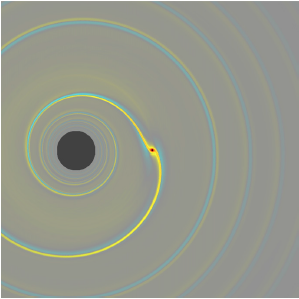
\includegraphics[scale=0.294]{figures/ch0/TypeI_Duffell}& \hspace{-0 pt}
%
 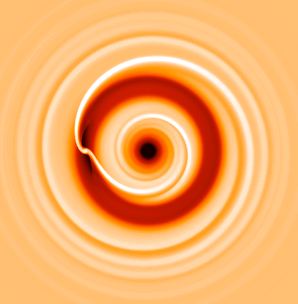
\includegraphics[scale=0.4]{figures/ch0/JupiterTypeII} &  \hspace{-0 pt}
%
 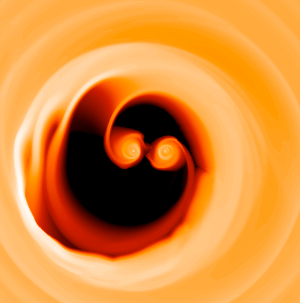
\includegraphics[scale=0.4]{figures/ch0/q1_CentralCav} 
\end{array}$
\end{center}
%\vspace{-0.35in}
%\caption{Snapshots of density from 2D hydrodynamical simulations for binaries on a fixed circular orbit, with increasing binary mass ratio from left to right ($q=10^{-6}, 10^{-3}, 1.0$). The Left panel is adopted from \citep{DM2012:gaps} and depicts the linear, Type I regime, the middle panel depicts teh Type II regime, and the right panel.} %
\caption{The left panel is for $q\equiv M_2/M_1 =10^{-6}$ (adapted from \citep{DM2012:gaps}), such a small secondary excites linear spiral density waves in the disk causing Type I inward migration of the binary. The middle panel is for a binary with $q=10^{-3}$, the dark ring in the orbit if the smaller BH is the low density gap leading to Type II migration. The right panel depicts the clearing of a central low density cavity around an equal mass binary.}
\label{Fig:IntroHydro}
\vspace{-0.2in}
\end{figure}
%%%%%%%%%%%%%%%%%%%%%%%%%%%%%%%%%%%%%%%%%%%%%%%%


\cite{LinPapa:1979a}, \cite{GT79}, and \cite{GT80} laid the groundwork for
disk interactions with very small mass ratio systems, where the response of
the binary and disk can be explored with linear perturbation analysis. In this
case, the secondary launches linear spiral density waves from the locations of
Linblad resonances in the disk \citep{LyndenBellKalnajs:1972}. Summing
contributions from torques exerted on the disk at these resonances,
\cite{GT80} were the first to show that the back-reaction of the disk
perturbations onto the binary cause the binary orbital separation to change.
For normal disk parameters (\emph{e.g.} outward decreasing disk density and
pressure), inward torques on the secondary from the outer Linblad resonances
outweigh the outward torques on the secondary from the inner Linblad
resonances, and inward `migration' (orbital shrinkage) occurs
\cite{Ward:1986}. This process, where linear spiral density waves are launched
by the secondary and cause the binary's orbit to shrink, is called Type I
migration \citep[See also][]{MeyerVernetSicardy:1987, Ward:1997, Tanaka:2002}.
Hence, the solutions to the equations of hydrodynamics, for disks perturbed by
a small mass ratio binary, consist of wave solutions launched form the
position of the secondary. In the frame of the binary, these waves have a
stationary phase and once they propagate into the disk on both sides of the
binary, the disk approaches a static solution which follows the secondary
component as it slowly changes its orbital radius and possibly eccentricity
(See Figure \ref{Fig:IntroHydro}) \citep{GT80, Ward:1988, GoldriechSari:2003}.





When the binary mass ratio is large enough, the spiral density waves launched
in the disk become non-linear at only a short distance (less than a disk scale
hieght) from the secondary \citep{GoodmanRafikov:2001}. The waves steepen into
a shock and deposit angular momentum to the disk material in the co- orbital
region of the secondary \citep{DongRafI:2011, DongRafII:2011, LinPapa, chapter3}. This
process clears a low density annulus in the orbit of the secondary.
\cite{LinPapa:1986b} were the first to point out that if such a gap is formed,
the secondary will be locked into the radial flow of the disc, migrating at
the viscous inflow rate. Such migration, when a gas barrier is formed around
the binary is called Type II migration \citep[see also][and Chapter 3]{Ward:1997, KleyNelson:2013, othertypeIIrefs}



Another important difference between different binary+disk systems is the
total gas resvoir. Analytical work by \citep{SyerClarke:95, Ivanov:1999}, in
one dimension,\footnote{averaging disk height and azimuth} showed that in the
non- planetary case, the Type II rate would eventually slow on scales where
the mass of the disc becomes smaller than the mass of the migrating binary
component. The argument being that there is no longer a large enough angular
momentum reservoir in the gas to shrink the binary separation on the viscous
timescale, hence, this `secondary dominated migration' would cause a pileup of
gas behind the secondary and the gas interior to the secondary's orbit would
drain onto the primary creating a central cavity devoid of gas and possibly
halting accretion onto the binary. Other 1D arguments \citep{other1Darguments} and even early 2D smoothed particle hydrodynamics (SPH)
simulations simulations \citep{Artymowicz:1991} concluded that the outward
torques from the binary would clear a cavity around most binary systems in the
Type II regime.


This picture, while laying the goundwork, has been greatly altered by work in
the intervening two decades, notably by the advent of two-dimensional
numerical, hydrodynamical simulations which capture the full non-axisymmetric
nature of the binary disk interaction, and allow global, time-dependent
solutions. The first of such numerical calculations was carried out in
\cite{AL94} and \cite{ArtyLubow:1996} who ran SPH simulations to
test analytic work that predicted the sizes of circumstellar disks in binaries
and the sizes of the central cavities surrounding the stellar binaries. These
SPH simulations showed that particles, in the form of streams tidally ripped
from the edge of the cavity wall, could indead flow past the binary tidal
barrier and reach the binary components. The ability of gas to flow past the
tidal barrier is of two-fold importance. First, it can allow high levels of
accretion onto the binary, which could generate a bright EM signature of the
binary, and second, it affects migration (and hence merger) rates of binaries
in gas disks \citep{DuffellFTV:2014}. The implications of both are currently areas
of active research. 




This picture, fails to account for mass flow across the gap along
horshoe orbits in the full dimentionlity of the problem. Recent work, using 2D
viscous hydrodynamical simulations has shown that mass flow accross the gap,
can allow the secondary to migrate at a rate depedent on disk parameters
(denisty, temperature, pressure), and limited by a maximum migraton velocity
which can be greater than the viscous rate \citep{Edgar:2008, DuffellFTV:2014,
DurmannKley:2015}. The mechanisms which dictate the migration rate of gap
openeing planets in the full two and three dimensional pictures is a topic of
ongoing work.


Additionally Chapter 3 of this thesis shows that the clearing of a central
cavity is not necessarily due to secular effects as in the picture of disc
dominated migration \cite{SyerClarke95}. Chapter 3 provides evidence that
the clearing of an annulus in the orbit of the secondary gives way to a much
more violent clearing of a \emph{central cavity} for mass ratios above $q
\sim0.04$.

Chapters 2 and 3 show also that the Type I to Type II regimes are not the only
that depend on mass ratio. For binary mass ratios above $q\sim0.04$, a mass
ratio well into the Type II regime for thin disks, the clearing of an annulus
in the orbit of the secondary gives way to a much more violent clearing of a
lopsided, \emph{central cavity} and time dependent bahavior. From mass ratios
$q \sim 0.3$ the lopsided central cavity is highlighted by an orbiting
overdensity at its inner wall. Chapters 2 and 3 provide more details on these
transitions and their importance for observing MBHBs.




The work in this thesis focuses on the implications for accretion onto the binary. Hence we now summarize the recent work on this front.


\cite{Haysaki:2007} conducted the first 3D-SPH simulations that specifically
targeted MBHB systems with the intent to measure accretion rates onto the
binary. \cite{Haysaki:2007} runs simulations of binaries with mass ratios
$q=1.0$ and $q=0.5$ and binary ecentricities $e=0.0$ and $e=0.5$ for up to 60
binary orbits. They find that streams are indeed pulled into a central, low
density caviy forming a triple disk system \citep{Hayasaki+2008} consisting of
the circumbinary disk and mini-disks around each binary component. The streams
promote accretion onto the BHs at rates as high as a tenth of the Eddington
rate. For eccentric binaries, \cite{Haysaki:2007} found a strong modulation in
the accretion rate at the binary orbital period. 
%Cons - run for a short time at low resolution, injection of particles at r=1.65 seems artificial

The SPH simulations of Hayasaki were soon succeeded by the 2D, grid based,
adaptive mesh refinment simulations of \citep[][hereafter MM08]{MacFadyen:2008},
 run for 1000's of binary orbits (greater than a viscous
time at the position of the binary). These higher resolution simulations,
using the FLASH code \citep{Fryxell:2000}, are more adept at capturing
supersonic dynamics in the vicinity of the binary (shocks). Though
MM08 cut out the inner region of the domain containing the
binary, they measure accretion rates into the inner boundary which is inside
the low density (besides the streams) central cavity set by the initial
conditions. The high resolution simulation of MM08, for an
equal mass binary, found new behavior: the elongation of the central cavity
which results in high levels of accretion into the inner simulation boundary.
The resulting periodogram of the accreation rate  has the strongest peeks at a
low frequency peak near $4.5 \times$ the binary orbital period and at twice
the binary orbital period. They not discussed in MM08, the cause of accretion
variabiltiy at these timescales is elucidated in Chapter 2 of this thesis and
also \citep{ShiKrolik:2012} below.


Further SPH studies of MBHB systems were conducted by \citep{Cuadra:2009} who
3D simulations at a resolution $10 \rightarrow 100$ times higher than that of
\cite{Haysaki:2007} for marginally self-gravitating discs with a binary mass
ratio of $q=0.3$ and a simple cooling prescription for the gas. They do not
find elongation of the cavity as in MM08, though this could be due to the
short amount of time for which the simulations are run, $\sim 200$ orbits, or
the resolution loss that SPH simulations suffer in low density regions (namely
the dynamically import cavity edge of the circumbiary disk).
\citep{Cuadra:2009} do find an accretion rate variable at the orbital period
and a propensity for the gas disk to excite binary eccentricity.
\citep{Cuadra:2009} also finds that the smaller has a larger ($\times 2$)
accretion rate than the secondary due to its closer proximity to the edge of
the central cavity.


\citep{Roedig:2011:trqs} carry out similar simulation to \citep{Cuadra:2009}, except they start the binary at different initial eccentricities $e_0$ finding that eccentricity damps for $e_0 \gsim 0.6$ but is excited for $e_0 \lsim 0.6$, suggesting the existence of rather large a preferred binary eccentricity. \citep{Roedig2012:eccevo} consider different disk thermoydnamics and different accretion (sink) perscriptons. In both cases the accretion rates onto these eccentric binaries  found to have periodicity at the binary period and its harmonics, but also at lower frequency disk periods and beat frequencies between disk and binary periods.


The first magneto-hydrodynamical (MHD) simulations of the circumbinary disk
were carried out by \cite{ShiKrolik:2012} with a grid based code.
\cite{ShiKrolik:2012}  perfomed both 2D hydrodynamical and 3D MHD simulations
of an equal mass binary on a circular orbit with a similar setup to
\citep{MacFadyen:2008}. Despite a higher overall accretion rate due to larger
viscous stresses generated by the Magneto-rotational instability (MRI),
\cite{ShiKrolik:2012} find similar results to MM08, in that they also find the
growth of a lopsided central cavity (elongated with a cavity wall
overdensity), which generates variable accretion into the central simulation
domain. The variablity of the accretion rate is in agreement with MM08,
exhibiting a long period variation at the period of gas orbits int the cavity
wall and a second period at twice the binary orbital period (due to the
symmetry of an equal mass binary). \cite{ShiKrolik:2012} provide evidence that
the cavity lopsideness is due to the kinematics of stream impacts and
recycling of the cavity wall overdensity: the cavity wall overdenisty
periodically shears apart, causing a lump to orbit around the cavity, feeding
streams which are flung out of the cavity again to generate the cavity wall
overdensity. \cite{ShiKrolik:2015} have extend upon the above work by
considereing a range of binary mass ratios, finding qualititve agreement with
\cite{DHM:2013:MNRAS} and \cite{Farris:2014} discussed below.

MHD simulations by \citep{Noble+2012} incorporate post-Newtonian corrections
to the disk hydrodynamics and binary orbital decay in order to track the disc
response through binary inspiral. \citep{Noble+2012} find that gas can follow
the binary down to separatios of $\sim10M$ with $10 \rightarrow 20\%$
reduction in accreation rate. They also find a lopsided central curcumbinary
disk cavity, in agreement with MM08, \citep{ShiKrolik:2012}, and the works
that we discuss next.

Chapter 2 of this work \citep{DHM:2013:MNRAS}, extends the work of MM08 (using
the same numericla code and a similar numerical setup) by considering not only
equal mass binaries but range a mass ratios from $q=0.01 \rightarrow 1$. The
qulatative results of disk response and accretion rate variability found in
MM08 and \citep{ShiKrolik:2012} are reproduced and compared to the magnitude
of accretion for a point mass. By varying $q$, however, a landscape of
accretion variabiltiy and mangitude is uncovered and discussion of its use for
MBHB searches is discussed.

\citep{Farris:2014} extended the work of \citep{DHM:2013:MNRAS} by adapting the
moving mesh code DISCO \citep{Duffell:2011:TESS,
DuffellMHDDISCO:2016} to track, for the first time, gas dynamics in the
vicinity of the binary components using a grid based (rather than an SPH)
code. \citep{Farris:2014} finds results in agreement with MM08 and
\citep{DHM:2013:MNRAS} and finds also that the relative accretion rate onto
each black hole is a function of mass ratio, dominated by the secondary from
$0.05 \leq q < 1$. 


For the equal mass case \citep{Farris:2015:GW} considered
the effects of gravitaional wave decay on the CBD system showing that gas
could indeed follow the binary to small separations causing variable accretion
up until merger, contrary to previous lore that gas should be left behind in a
`decoupling phase' by a binary that is quickly merging due to GW emission.
Finally \citep{Farris:2015:Cool} implemented a simple cooling prescription in
DISCO (previous work being for isothermal disks) showing that the variability
of the accretion luminosity should indeed follow what was predicted in
previous works for the variabiltiy of the accretion rate.



Recent work has examined the nature of gas temperature on accretion rates,
both \cite{YoungClarke:2015} and \cite{RagusaLodato:2016} use SPH codes (2D
and 3D repectivley) to simulate a range of binary mass ratios above $q=0.1$
and vary the gas temperature. In these simulations, the gas temperature
manifests in the form of the disk vertical height to radius aspect ratio,
$h/r$ which, in vertical hydrostatic equilibrium, is equal to the ratio of the
sound speed to the gas angular orbital frequency at distance $r$ from the
system barycenter. A thicker disk, is hotter and has larger pressure forces.
Both studies find that, while simulations in the literature (using $h/r \sim
0.1$) accrete at near the value for a single BH, more realistic, colder AGN
discs ($h/r \sim 0.01$) should accrete at much lower rates. Though
interesting, the robustness of these results remains to be seen as numerical
difficuties arise in cold disks, especically when using SPH codes \citep{}.


Notably, \citep{RagusaLodato:2016} simulations capture the lopsided disk
behavior with a circular binary. Except for a study which considered an
eccentric binary \citep{Dunhill+2015}, no SPH simulations have captured the
lopsided disk behavior. It is not yet clear however what has allowed this
change. The SPH works to date are computed with different numerical codes, at
different resolutions, and for different total numbers of binary orbits.


In addition to prograde disks in the plane of the binary, some groups have alse considered retrograde disks \citep{Nixon+2011, ReodigSesana:2014, BankertShiKrolik:2015, AmaroSeoane:RetroDiscs:2016} and the alignemnt or tearing of warped disks \citep{Nixon+2012, Hayasaki+2013, Nixon+2013, DoganNixonKingPrice:2015}.

As a final note in this review of numerical simulations of CBDs, full MHD
simulations in general relativity (GRMHD) have been carried out by
\cite{FarrisLiuShap:2010:Bondi, FarrisShap:2011, FarrisGold:2012,
Gold:GRMHD_CBD:2014, Gold:GRMHD_CBDII:2014} in the regime just before merger,
showing also that accretion rates can be of order the rate expected onto a
single BH, periodic, and the gas can follow the binary down to separations of
order a few $M$, allowing the binary to be bright up until merger.


% Stil need to add:
% Noble
% MunozLai:2016 - ecc stars accretion rates




%%%Observations
\subsection{Observations of MBHBs}

%%%%%%%%%%%%%%%%%%%%%%%%%%%%%%%%%%
%%%FIGURE doppler candidates
%%%%%%%%%%%%%%%%%%%%%%%%%%%%%%%%%%
\begin{wrapfigure}{R}{0.5\textwidth}
%\begin{figure}
\begin{center}
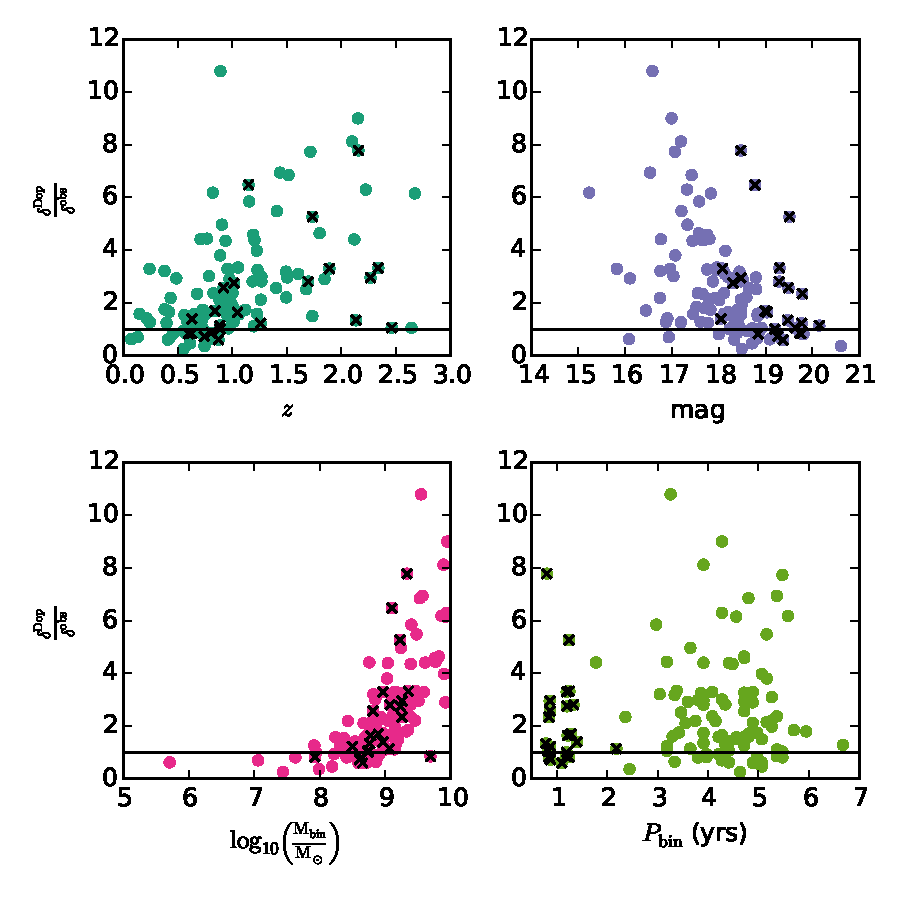
\includegraphics[scale=0.55]{figures/ch0/PTF_xsiGtr1_vs_z_M_P_alph_I90} 
\end{center}
\caption{A subest of the MBHB candidates from \citep{Graham+2015b} and \citep[][denoted by black x's]{Charisi+2016} for which spectral slopes are measured and the magnitude of variabiltiy form Doppler boosting can be estimated. From left to right, top to bottom, the ratio of predicted Doppler variability amplitude to observed variability amplitude is plotted vs, redshit, average optical magnitude, log mass, and observed period. Candidates above the horizontal black line are possible Doppler beaming MBHB candidates.}
\label{Fig:Contour}
%\end{figure}
\end{wrapfigure}
%%%%%%%%%%%%%%%%%%%%%%%%%%%%%%%%%%%%%%%%%%%%%%%%


As discussed, a motivation for the above theoretical calculations is to
determine the types of EM signatures that will identify MBHBs in the inspiral
regime. Searching for MBHB by searching for periodically varying AGN has been
proposed before by MM08, \cite{Haiman+2009}, and by HKM09.
 

HKM09 propose that close MBHBs can be indentified in Quasars by their production of EM emission moduated at the binary orbital period. Under this assumption they compute the duty cycle of MBHBs with periods observable in human lifetimes by computing the residence times of MBHBs at a given orbital period (binary separation) taking into account gas induced migration and also GW driven inspiral. Comparison of the residenc etime to the averge Quasar liftime allows HKM09 to predict the size of an EM time domain survey required to capture a specified number of MBHBs at agiven orbital period and luminosity.

%caluclate the duty cycle of MBHBs with 

%assume that MBHB can generate periodic EM signatues at the binary orbital period to predict the sample size of Quasars needed to detect a sample of MBHBs that should be needed based on Quasar lifetimes and gas + GW induced binary shrinkage. 




These predictions came to fruition only a year ago when the a group from
Caltech/JPL scoured 9 years of time domain optical photomoetry of
$\sim250,000$ quasars in the Catalina Real Time Transient Survey
\citep{CRTS1:Drake:2009, CRTS2:Djorgovski:2010, CRTS3:2011Mahabal,
CRTS4:Djorgovski:2011} attempting to characterize quasar variability. They
found a subset of periodically varying sources. The brightest of these sources
is PG 1302-102 which was identified as a close, $a \sim 0.01$pc separation
MBHB candidate, the first identified in this manner, and the closest reported
binary separation at the time \citep{Graham+2015a}. The second part of Part I
of this thesis uses the theoratical developments of the first half to
interpret the binary candidate PG 1302, finding that PG 1302 is most likely
described by a system with a disparate mass ratio where the smaller BH is
emitting most of the optical light and modulating it via relativistic Doppler
boosting.


Soon after the announcement of PG 1302, 110 more MBHB candidates, were picked
out of the CRTS for their periodic optical light curves \citep{Graham+2015b}
and then 33 more, at shorter periods \citep{Charisi+2016}, from the
Palomar Transient Factory (PTF) \citep{PTF}. In addition to these mass candidae
discoveries, a few single candidates were also announced from time domain periodicity arguments: A proported 


Follow up observations are needed to secure the nature of these candidates. As
Jules Halpern says: `periodicity is the easiest thing to prove in astronomy,
you just have to wait'. However, furhter evidence, across the
wavelengths can help pin down the mechanism driving such peridocity and work
must be done to place these MBHB in their full environment of gasy, dusty
active galactic nuclei. A full multiwavlength picutre of the variable MBHB
candidates must be peiced together. The final chapter of Part I (Chapter 5) is
a beginning to this process, presenting a model for the infrared variability
expected from dust reverberation by MBHBs that exhibit variable emission,
through either accretion variablitiy or anisotropic Doppler boosted emission.









% I want to note here 
% (0) intrinsic quasar variability
% (1) that the above searches might exclude binaries with multiple freqeuncies due to naure of wavelet analysis
% (2) Calculation of whether these 144 coudl be Doppler beamed plus figure.
% (3) MBHBs candidates claimed since with plusses or minuses
%  the search continues: \citep{Tamara:2015}
% 	spectroscopic methods:
% 	 BLRs:
% 		\citep{DecarliDott:2013:SpecMBHBcandI}
% 		 Halpern's group?
%      CBD cutoffs:

%      EM time domain
%       Graham a, b
%       Charisi+
%       Zheng, Z.

% (4) IR STUFF JUN ET AL AND CHAPTER 5!



%picture has been altered in the last decade...



% The advent of numerical simulations which capture the 2D, non-axisymmetric
% nature of the binary disk interaction also found that accretion onto the
% binary is not halted by a the torque barrier of the binary, rather accretion
% rates can even be increased from the point mass steady accretion case because
% teh binary can vioently pull streams of gass form a circumbinary cavity edge.
% The gas from these streams forms mini-disks around each binary component....
% explain accretion process with figure with vectors...

%Chapter 2 provides evidence for further birfurcations
%for near equal mass ratio systems and Chapter 3 elaborates on the physical
%mechanisms driving the more subtle of these transistion.








% %%% 1D Summary
% Early papers: 
% 	Type I: 
% 		Lynden-Bell and Kalnajs 1972 - resodnances and spiral arms in galactic setting
% 		Lin and Papaloizou 1979 a - angular momentum transport:Type I migration - tidal truncation of CBDs - application to dwarf novae
% 		GT 1980 - first to suggest migration - from resonant tides
% 		Meyer Sicardy - 


% 	Type II
% 		Syer Clarke Disk vs sec dominated - app to MBHBs
		
% 		b - Tidal truncation of CBDs applied to contact binaries and the formation of commensurable satellites in the solar system.
% 		Lin and Papaloizou 1986 a - full nonlinear interaction f disk and sattelite, self grav, range of c_s and nu - density wave propagation studied- applied to protoplanet and the primordial solar nebula
% 		b - dynamical evolution of the disk and the orbital migration of the protoplanet in a self-consistent manner is considered - Type II viscous evolution rate derived here - numerical stuff?
% 		Lin Papa 1993

% 	Gap Clearing 
% 		The above Lin Papa papers
% 		Arty and Lubow 1994, 1996
	
% 	Both:
% 	Hourigan Ward 1984
% 	Ward 1997

% 	Eccentricity excitation/damping
% 	Ward 1988
% 	Goldreich Sari 2003

% Present day answers to earlier work:
% Type I:
% Rafikov and Dong etc
% Duffell

% Type II:
% Edgar 2008
% FTV Duffell 2014
% Durman and Kley? 2015

%Syer and Clarke: secondary BH can clear a gap in the CBD, and bank up material behind it, causing a change in the spectarl and possibly continuum emission from the AGN. They also introduced the idea od Type II secondary dominated vs. disk dominated mogration.

% Retrograde and warps alignment
% Nixon+2011 - retro
% Nixon+2012 - alignment to retro of misaligned
% Hayasaki+2013 - warped/alignment
% Nixon+2013 - tearing up the disc - misaligned
% ReodigSesana:2014 - retro vs pro
% DoganNixonKingPrice:2015 - tearing up misaligned
% BankertShiKrolik:2015 - retro
% Amaro-Seoane+2016 - retro

% EMPHASIZE THE QUESTIONS IN THIS THESIS: Can accretion make EM signature of MBHB and can we use it to identify a pop of MBHB candidates?





































\section{Part II: Stellar Black Hole + Neutron Star Binaries}
%EMPHASIZE THE QUESTIONS IN THIS THESIS: What is the BH battery EM signature of non-disrupting NSBH binaries?
%

The merger of NSs and stellar BHs will generate GWs detectable by the Laser
Interferometer Gravitational-Wave Observatory \citep[LIGO][]{aLIGO:2015}.
Binaries with BHs will generate the highest amplitude GW signals \emph{e.g.}
Eq. \ref{Eq:BinStrain}, but a binary containing a NS has the most potential to
produce a bright EM signal, making BHNS systems especially interesting sources
of EM+GW emission.


%%%%%%%%%%%%%%%%%%%%%%%%%%%%%%%%%%
%%%FIGURE BHNS TDs
%%%%%%%%%%%%%%%%%%%%%%%%%%%%%%%%%%
\begin{wrapfigure}{R}{0.4\textwidth}
%\begin{figure}
\begin{center}
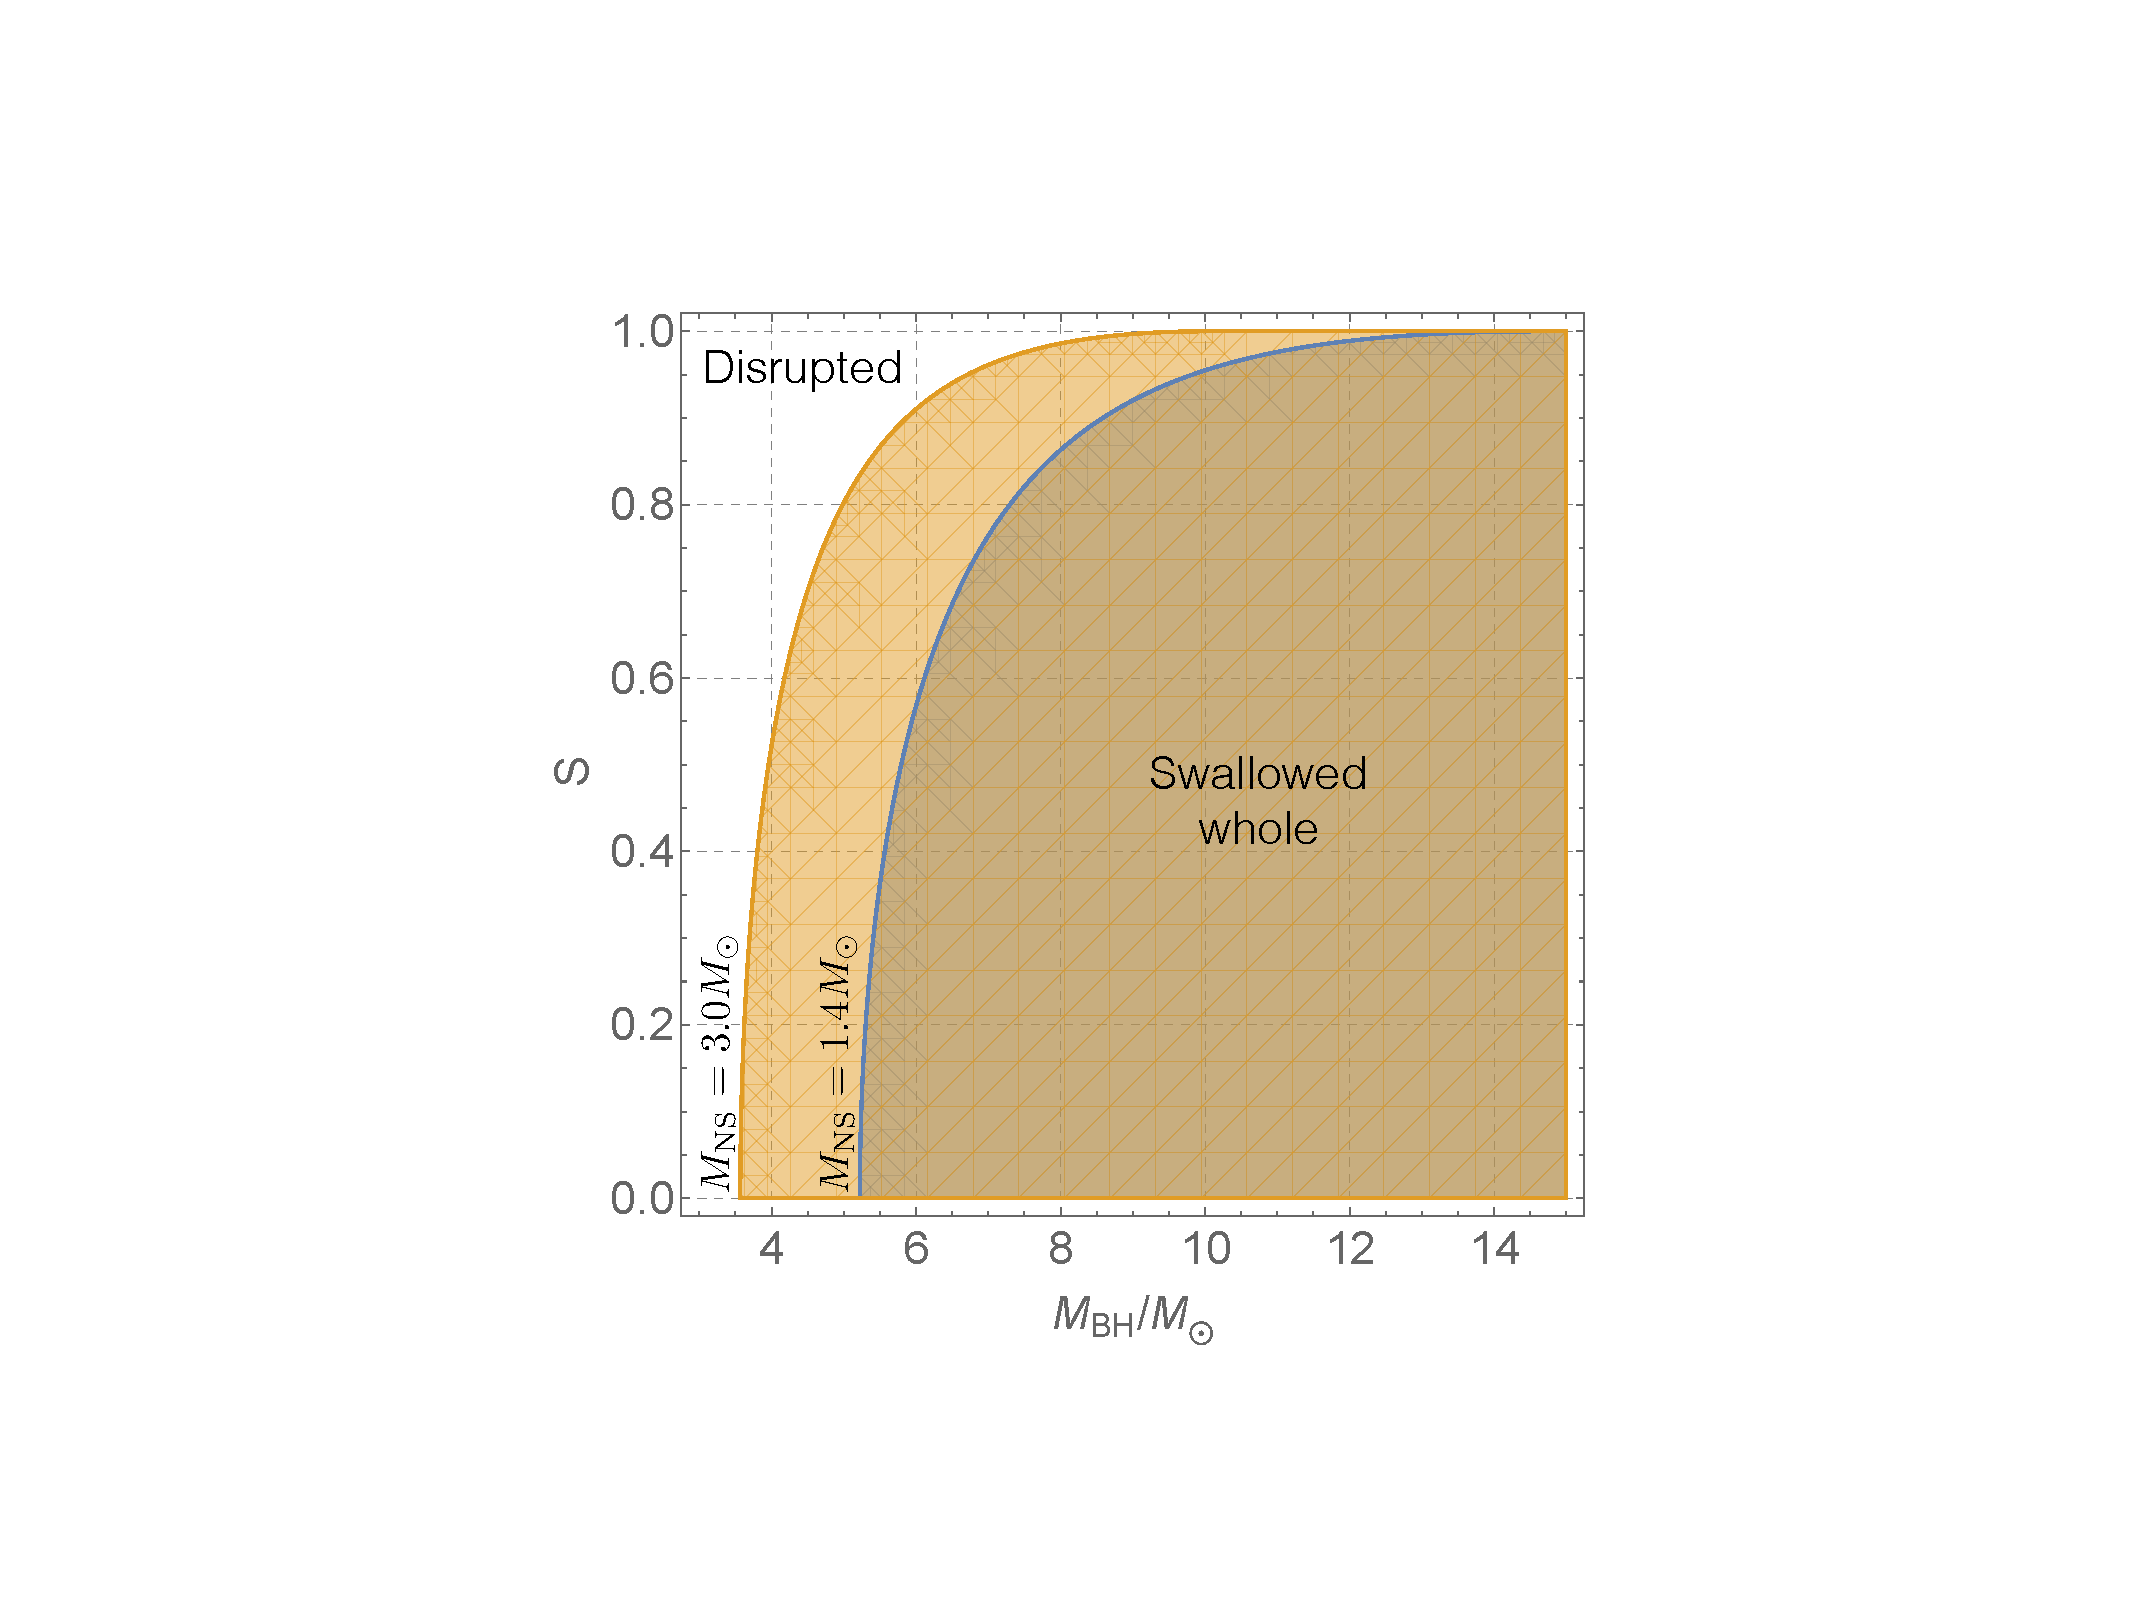
\includegraphics[scale=0.33]{figures/ch0/BHNS_TDs} 
\end{center}
\caption{Approximate values of black hole mass and spin for which a companion neutron star would be disrupted outside of the black hole horizon. Each of the two regions are for the labeled neutron star masses spanning the range of theoretical limits and for a neutron star with radius of 10km.}
\label{Fig:Contour}
%\end{figure}
\end{wrapfigure}
%%%%%%%%%%%%%%%%%%%%%%%%%%%%%%%%%%%%%%%%%%%%%%%%

The tidal disruption of a NS by its BH partner could generate a $\gamma$-ray
burst after merger \citep{NPP:NSBH_GRB:1992}. However, it is under-appreciated
that most BHs should be large enough to swallow their NSs
whole, causing the mergers of most BHNS binaries to be dark. Figure 
\ref{Fig:NSBH_TDs} plots the simplest approximation for the disruption,
\begin{equation}
 r_T \approx \left( \frac{M_{\rm{BH}} }{ M_{\rm{NS}}} \right)^{1/3} R_{\rm{NS}} \geq r_H(S) 
 = M_{\rm{BH}} + \sqrt{M^2_{\rm{BH}} + S^2},
\end{equation}
which requires that the disruption radius be outside of the BH event horizon
with dimensionsless spin $S$ (using natural units for the black hole horizon
radius). \ref{Fig:NSBH_TDs} shows that, unless the BH has near maximal spin,
BHNS systems with $M_{\rm{BH}} \gsim 6 \msun$ will swallow the NS whole! This
is of course a crude aproximation which depends on the (unknown) equation of
state of the NS. More sophistaced approximations, however, do not find anything
drastically different \citep[\emph{e.g.}][]{Foucart:2012}.


Although the distribution of BH masses which will merge with
a NS is unknown, it is interesting to note that the BH mass distribution
inferred from BHs in X-ray binaries peaks around $8 \Msun$ \citep{Ozel:2010}
and the only known BH binary consisted of BHs with masses $\sim 30 \Msun$, which
would certainly swallow a NS hole. Though suggestive, it is important to keep
in mind that each of these formation channels may be independent, and not
applicable to a BHNS system.

As additional motivation, LIGO is the most sensitive at a frequency of $\sim
200$ Hz, this is the gravitational wave frequency at coalescence for a NS of
mass $1.4 M_{\Msun}$ in a circular orbit with a BH of mass few $\sim100
\Msun$. If such binaries occur in nature, they have the potential to be high
signal to noise LIGO detections, and will certainly not disrupt the NS. The
above motivates an exploration of EM counterparts to non-disrupting NSBH
systems.


A possible pathway for bright EM emission by non-disrupting BHNS mergers is
through the electromegnatic interaction of the NS magnetosphere and the BH
event horizon. 

Paragraph about all the diff astro mechanisms for UIs.
% The NSBH system behaves analogously to a unipolar inductor, which has been investigated in application 
% to a number of other astrophysical systems, \textit{e.g.} Jupiter and 
% its moon Io \citep{GLB:1969}, planets around white dwarfs \citep{Li:1998} and main sequence stars \citep{LaineLinI:2012,LaineLinII:2012}, 
% binary neutron stars \citep{Vietri:1996,Piro:2012, DLai:2012, Palenzuela:2013}, 
% compact white dwarf binaries \citep{Wu:2002, Dall'Osso:2006, Dall'Osso:2007, 
% DLai:2012}, BHs boosted through magnetic fields 
% \citep{Lyut:2011, Penna:2015}, and the Blandford-Znajek (BZ) mechanism \citep{BZ:1977} for a single BH spinning in a magnetic field  \citep[for recent numerical work on the BZ mechanism see \textit{e.g.}][]{PalenzuelaBZ:2011, Kiuchi:2015}. The calculation for NSBH systems, 
% already presented in Ref.\ \cite{McL:2011}
% and confirmed in the detailed relativistic analysis of
% Ref.\ \cite{DorazioLevin:2013}, as well as the numerical calculations
% of Ref.\ \cite{Paschalidis:2013}, gives the scaling of power available
% for conversion into electromagnetic luminosity. In the next section we
% will consider the implications of throwing this power into luminous
% elements in the BHNS circuit.

To introduce this mechanism, I want to first introduce a
similar, though subtle example of the Faraday-Disk. The Faraday disk is a type
of unipolar inductor constructed by placing a conducting rod through the
center of a conducting disk, and running a wire from the top of the rod to the
outer edge of the disk, where a sliding contact completes a circuit (see
Figure \ref{Fig:FDschem}). Tracing a magnetic field perpendicularly through the disc, and
spinning the disk generates a elecromotive force, $\xi$. We can compute the
voltage drop from the center of the disk, to the edge of the disk, from
Faraday's law 
\begin{align} 
\xi = - \frac{1}{c}\frac{d}{dt}\int_{\Sigma(t)}{\Bvec \cdot d\Avec} 
\end{align} 
where the circuit bounds an open, time-dependent surface $\Sigma(t)$. At first
glance, it seems that the emf should be zero, as the obvious loop (loop $a$ in
Figure \ref{Fig:FDschem}) connecting wire to disk to rod has zero magnetic
flux. However, Faraday disks do generate an emf, and this is easily verified
by considering the Lorentz force on electrons. To see this from Faraday's law, recall two restrictions in our
choice of the open surface of integration $\Sigma(t)$: 1) $\Sigma(t)$ must be bounded by the closed loop through which the emf is computed, and 2) $\Sigma(t)$ must capture the relative motion of the circuit.
%\begin{enumerate} 
%\item $\Sigma(t)$ must be bounded by the closed loop through which the emf is
%computed. 
%\item $\Sigma(t)$ must capture the relative motion of the circuit.
%\end{enumerate}
The key is in the second point: the part of the circuit that starts in the
disk must move along with the spinning disk, otherwise you implicitly assume
that the sliding contact and the disk are not in relative motion - but they
are by construction.


%%%%%%%%%%%%%%%%%%%%%%%%%%%%%%%%%%
%%%FIGURE Faraday Disk
%%%%%%%%%%%%%%%%%%%%%%%%%%%%%%%%%%
\begin{wrapfigure}{R}{0.4\textwidth}
%\begin{figure}
\begin{center}
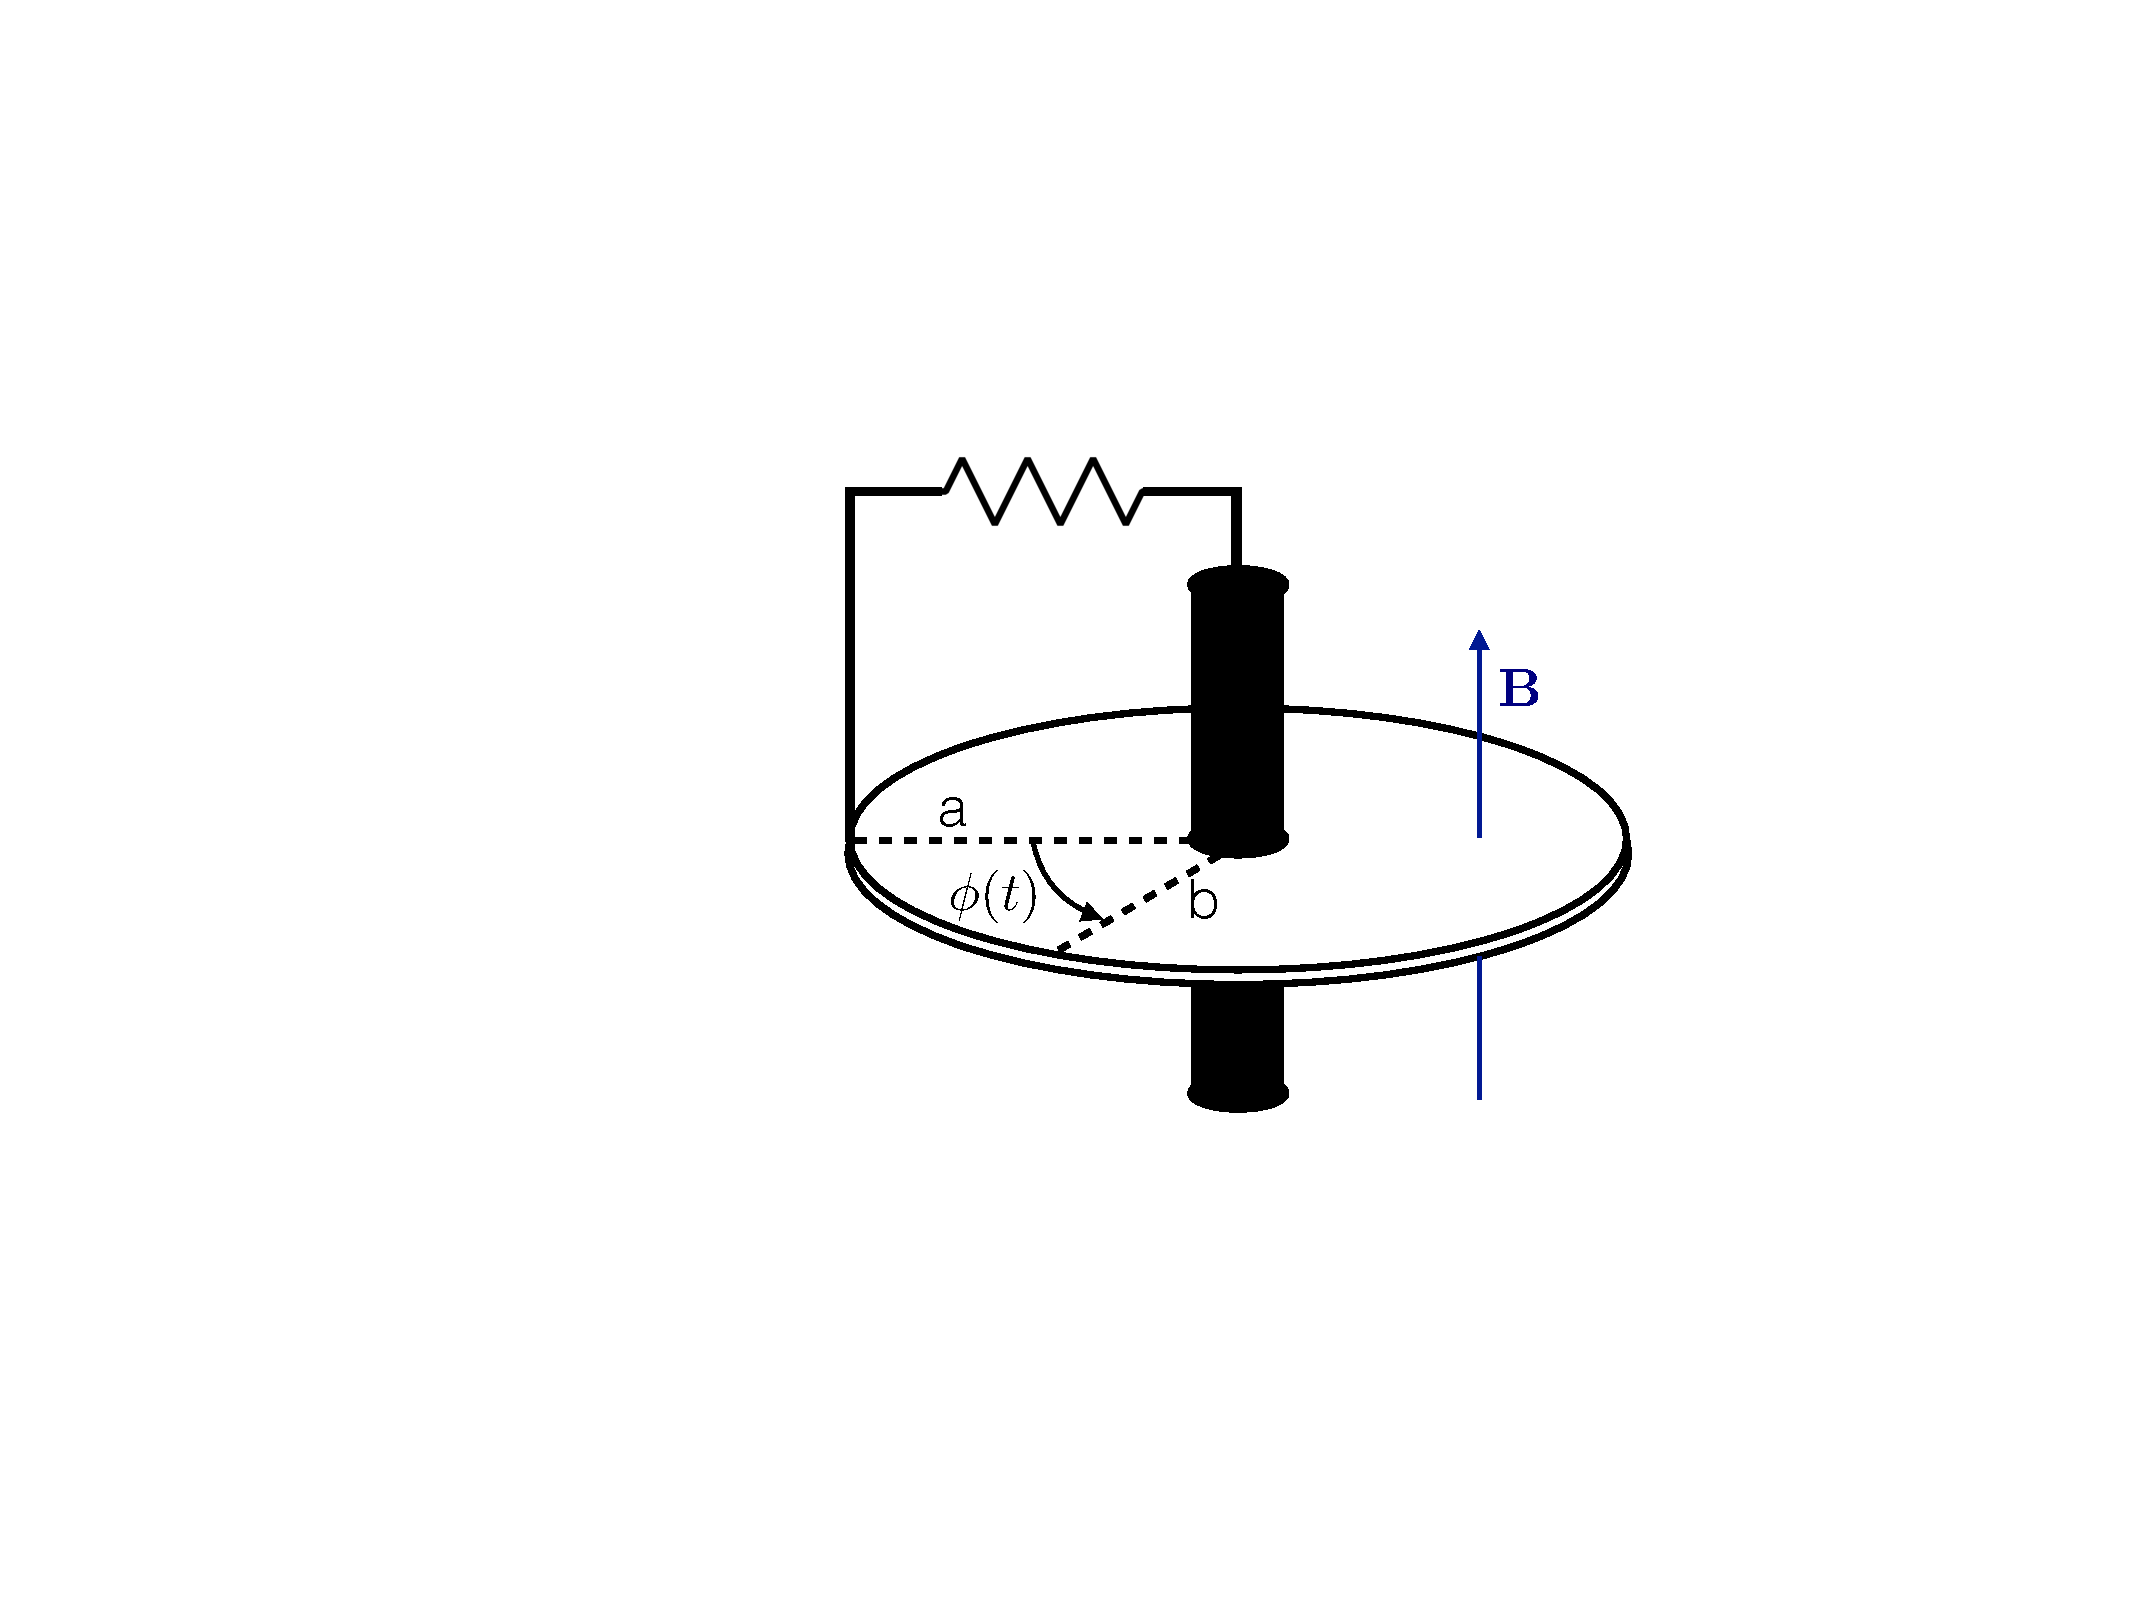
\includegraphics[scale=0.33]{figures/ch0/UI_schematic} 
\end{center}
\caption{Schematic of a Faraday Disk (unipolar inductor).}
\label{Fig:Contour}
%\end{figure}
\end{wrapfigure}
%%%%%%%%%%%%%%%%%%%%%%%%%%%%%%%%%%%%%%%%%%%%%%%%


To calculate the emf, choose loop $b$ in Figure \ref{Fig:FDschem} which moves
along at the rate of the spinning disk, $\Omega = d\phi/dt$. Say that the
radius of the disk is $R$ and the uniform magnetic field tracing the disk is $B$, then, working in polar coordinates $(r, \phi)$,
\begin{align}
\xi_{\rm FD} &= - \frac{1}{c} \frac{d}{dt} \int_{\Sigma(t)}{\Bvec \cdot d\Avec} =  - \frac{1}{c} \int^{\phi(t)}_{0} \int^{R}_{0}{B r dr d\phi}  \\
&= - \frac{1}{c} \int^{\phi(t)}_{0}{\frac{1}{2}\frac{\partial B R^2}{\partial t} d\phi} -  \frac{1}{c} \frac{B R^2}{2} \frac{d\phi}{dt}  = -\frac{B R^2}{2c} \Omega
\end{align}
where we have used Liebniz's rule of for integration with a time changing limt of integration. 

Remarkably, it turns out that the Faraday disk behaves similarly to a BH
moving through a magnetic field. The analogy is spelled out in \S \ref{}, but
if we take for now that the BH orbitting the NS acts as a conductor with size
equal to its event horizon \citep{MPBook}, then we can calculate the emf
generated by the NSBH system. 

All of the above reasoning holds for the BH battery, but instead of sliding
wires, we have moving B-feild lines which both act as wires (because electrons
are bound to them) and also generate the magnetic flux through the moving BH
horizon. Take our circuit in the BH-battery case to be the B-field gong form NS surface to a time dependent boundary on the BH horizon. Take the B field to be
that of a dipole attached to the NS, $B = B_{\rm NS} R^3_{\rm NS} r^{-3}$ and
consider two field lines separated by distance $R_H$ and moving in the $x$
direction relative to the horizon at speed $v_f$. then we find an result for
the horizon voltage analogous to the Faraday Disk case, and nearly identical
to that derived in \S \ref{7.1.1},
\begin{align}
\xi_{\rm BH} &= - \frac{1}{c}\frac{d}{dt} \int_{\Sigma(t)}{\Bvec \cdot d\Avec} =  - \frac{\pi R_H}{c} \int^{v_f t}_{0} {B(r) dx}  \\
&=  - \frac{\pi R_H}{c}  \int^{v_f t}_{0}{ \frac{\partial B(a)}{\partial t} dx}  - \pi R_H B(r) \frac{v_f}{c}    \\
& \sim    -R_H \left[r \frac{\left(\Omega_{\rm bin}  - \Omega_{\rm NS}\right)}{c} + \frac{R_H\Omega_{BH}}{c}\right] B_{\rm NS}  \left( \frac{R_{\rm NS}}{r} \right)^3
\end{align}
which is the maximum voltage over one hemisphere. There an infinite number of these circuits at all times. 

In the case of the Faraday Disk, the energy which can be harvested
electromagnetically, \emph{e.g.}, by heating the resistor in Figure
\ref{Fig:FDschem} to light a bulb), comes from the energy put into spinning
the disk. In the case of a BHNS binary, the electromagnetic potential energy
of the induced horizon voltage comes from the binary orbital energy, and as
detailed in Part II of this thesis, the available electromagnetic energy could
power luminosities observable from galactic distance (kpc) out to comsic
distance (Mpc) depending on the NS magnetic field strength at merger.


This result, that NSBH binaries could power high luminosity EM counterparts
without disrupting the NS was first put forth by
\cite[ML11][]{McL:2011}. This work was then expanded upon by
Chapter 7 of this thesis \cite[DL13][]{DL:2013:PhRvD}, which finds relativistic
solutions for the dynamics of a magnetic dipole, in arbitrary motion outside
of a horizon. 

Numerical works have recently tackled this problem in general relativistic,
force-free simulations, which solve the Einstein-Maxwell equations in the
limit that $\Evec \dot \Bvec$ is everywhere zero, and hence there are no
accelerating forces on electrons \citep{Paschalidis:2013}. Both types of
simulations estimate the observable luminosity via a Poynting flux measured at
the outer edge of the simulation domain. The simulation estimates match the
analytic arguments of ML11 and DL13. However, a true understanding of the
emission from NSBH systems requires more than this; it requires a radiation
maechanism, somethign to stick into the BH-batterey circuit that will shine.

The emission of EM radiation ultimately must come from dissipation of the BH-
battery power in the joint BHNS magnetosphere. The classic paper by
\cite{GJ:1969} shows that if a spinning NS, immersed in its own magnetic dipole
field, generates an electric field with components perpendicular to the
magnetic field, then electrons will be ripped from the NS crust. The
acclerating electrons emit curvature radiaiton which interacts with the
electromagnetic field to generate pair electron-positrons pairs which go on to
genreate more curvature radiation and a pari cascade ensues. The pairs move to
screen accelerating electric field (components of $\Evec$ parallel to
$\Bvec$), until a force-free condition is met, and the NS is surrounded by the
magnetosphere of \citep{GJ:1969}. Such a situation halts dissipation of the BH-battery power. 

However, this does not stop pulsars from shining.  As \citep{RudSuth:1975} pointed out, the force free condition cannot always be sustained globally in the NS magnetosphere, for example, (). In these gaps, particles are still acceleratd and dissipation allows the release of EM radiation.

We assume that a similar situation is at play in the NSBH example. There need only be gaps in the forece free magnetosphere, or magnetic reconnetion (though I am not sure how this would occurr) to release the BH battery power. In Chapter 8, we envision such a mechansim, which results in a fireball soon after merger emitting in the hard x-rays and soft $\gamma$-rays. Recently a similar fate has been envisioned for the anlogous NS-NS system \citep{MetzgerNSNS:2016}. I am hopeful that both of these models will soon be tested by GW observations of coalescing NSBH and NSSN binaries. Stay Tuned.



%Palenzuela:2013


% These works have understood the energetics and mechanisms for generating
% electric potential in the inspiralling NSBH system, however they do not fully
% adress how this potential energy is relased as observable EM radiation.




% This analytic work has been tested by numerical simulations of the 

% Numerical simulations:
% Shapiro, Palenzuela for NS-NS: Full resisitive,
% general relativistic, MHD simulatiosn have also been carried out for merging
% NSNS binaries, where a similar unipolar inductor mechansim is at play
% \citep{Palenzuela..}.
% other theory:
% Lai
% Piro


% not jsut BHs, but planets WDs, any situtation wher a conducting surface moves through an astrophyiscal magnetic field.




% previous work on this...


% %magnetosphere phsyics
% While the BH batterey provides a power source, the mechanisms by which this power is dissipted is crucial for predicting observational consequences. 

% Dissipation in NS magnetospheres:
% GJ69, RS72, and Force Free?\\
% How does disipation ensue? - Reconnection, Gaps?

% Conclusions:
% %Problems to surrmount?
% How do we form close NSBHs?
% what are the NS field strengths at merger?\\

% %LIGO relation
% Review of Pop Synth for NSBH LIGO?\\
% prospects in the LIGO era









\section{Outline of thesis}  
The rest of this thesis is organized as follows.
Chapters 2 through 5 concern MBHBs. Chapter 2 presents hydrodynamical
simulations for idealized accretion flows around MBHBs on circular orbits. It
is shown that the accretion rates into the cavity cleared by the black holes
is traced by accretion streams which can feed the black holes at a rate
comparable to that of a single black hole. Furthermore it is shown that, for
non-extreme mass ratio binaries, the accretion rates are strongly modulated on
timescales which depend on the binary mass ratio. Chapter 2 further explores
the transition between strongly modulated accretion flows and steady flows
finding dynamical evidence for a transition in CBDs at a binary mass ratio of
1:25. Chapter 2 also explores the dependence of this transition on disk
pressure and viscosity. Chapter 3 utilizes the mass ratio dependent theory of
accretion rate variability worked out in Chapters 2 and 3 to interpret the
MBHB candidate PG 1302-102. Chapter 4 extends this interpretation of PG 1302
in the specific case that PG 1302 is a binary with mass ratio below the CBD
transition of Chapter 3. In this case, a compelling interpretation for the
periodic light curve of PG 1302 is found in the relativistic Doppler Boost
model. Chapter 5 places the Doppler boost model in the larger setting of AGN,
developing a toy model for the reverberation of optical and UV light by a
surrounding dust torus. This model is fit to the IR light curve of PG 1302,
finding agreement.

Chapters 6 and 7 concern the interaction of NS magnetic fields and a BH
horizon. Chapter 6 presents exact relativistic solutions for the vacuum
electromagnetic fields of a magnetic-dipole source in arbitrary motion near an
event horizon. The solutions are used to interpret and elucidate the
electromagnetic circuit which may be hooked up to create high energy EM
emission in a BHNS binary. Chapter 7 examines the nature of this high energy EM emission by hooking up a circuit of Chapter 6 to a metaphorical light
bulb which manifests in the form of a pair fireball brought on by high energy
curvature radiation.



















%------------------------------------------------------------%
%-------------------------OLD STUFF--------------------------%
%------------------------------------------------------------%
%At 09:50 UTC on September 14, 2015, the laser interferometer
%gravitational wave observatory (LIGO) detected gravitational waves from the
%merger of two $\sim 30 \msun$ black holes. This first direct detection of
%gravitational radiation (gravitational waves or GWs for short) and first
%unequivocal confirmation of the existence of black holes has ushered in a new
%era of gravitational wave astronomy. In this era, multi-wavelength and multi-
%messenger (photons, gravitons, neutrinos) observations of GW sources will be
%crucial for making the next steps to...


%, \textit{e.g.}, the vicinity of merging black holes and neutron stars.
%, including the formation of close binaries on multiple scales,
% such as accretion and electromagnetic field dynamics, that occur




%telling us that we would need to put a detector near the event horizon of a matter distribution with typical velocities near the speed of light in order to experience of order unity perturbations to the spacetime metric. Since these conditions are only found around black holes, we can also conclude that, in building a gravitational wave emitter, black holes are the golden standard in components. As we have not yet built black holes in a laboratory, we look to astrophysical sources. The best known astrophysical sources which approach the dimensions discussed above are The mergers of two (or more) compact objects, namely black holes, neutron stars and white dwarfs \citep{}, Cosmic Inflation \citep{}, Cosmological defects such as cosmic strings \citep{}, Neutron star mountains \citep{}, and core-collapse supernovae \citep{}.
%
%This also tells us that the largest possible gravitational waves are generated by mass distributions with velocities approaching the speed of light and packed into a space the size of a black hole event horizon. GWs with larger amplitudes are shielded by an event horizon. Hence, in building a gravitational wave emitter, black holes are the golden standard in components. As we have not yet built black holes in a laboratory, we look to astrophysical sources. The best known astrophysical sources which approach the dimensions discussed above are
%\begin{itemize}
%\item The mergers of two (or more) compact objects, namely black holes, neutron stars and white dwarfs \citep{}. At the time of writing this class of sources is the only to have been detected in gravitational waves\citep{GW091415}. Two such binary systems are the subjects of this thesis.
%\item Inflation \citep[\textit{e.g.}][]{Guzzatti:2016}.
%\item Cosmological defects such as comsic strings  \citep[\textit{e.g.}][]{}.
%\item Neutron star mountains  \citep[\textit{e.g.}][]{}.
%\item Supernovae  \citep[\textit{e.g.}][]{}.
%\end{itemize}

%A final type of GW detector aims to measure very low frequency ($\sim
%10^{-16}$ Hz) gravitational radiation through its imprint on the polarization
%of the cosmic microwave background (CMB). Though we will not discuss it here,
%the search for such polarization of the CMB is actively being pursued out by
%various competing groups \citep{}.







%The broad motivation of this thesis is to examine astrophysical sources of
%gravitational radiation in the context of their astrophysical environments
%and, in this way, deduce the possibilities for EM observations of GW events
%which could produce multi-messenger events or serve as pure EM observations
%identifiers of GW events in absence of a GW detection.

%Removing the simplification of pure vacuum General Relativity, we placing the
%most promising sources of GW radiation into their expected astrophysical
%environments, and what EM signatures do gravitational wave sources generate
%and what can they tell us? A goal of this thesis is indeed to elucidate this
%question for two specific cases of neutron star black hole (NSBH) binaries
%and massive black hole binaries (MBHBs). In order to place this goal in
%greater context, we first survey the known literature on EM signatures of GW
%sources, specifically the inspiral and coalescence of compact objects.

%For brevity we include only those related to mergers of compact objects. In
%any event, it is useful to consider two categories

%The term EM signature of a GW source is a general term which includes
%observable EM emission that is coincident with a GW detection, and also
%events which occur well before or after the GWs, but can still provide unique
%evidence for the system. The former we refer to as EM counterparts, while the
%latter we call EM tracers. Splitting into these two categories:


%\paragraph{Some EM counterparts of compact object mergers} When an EM signal
%is observable in close temporal proximity to an observable GW event, we call
%this an EM counterpart because it is a counterpart to the GWs (I suppose we
%could just as likely call this a GW counterpart to an EM source). Examples in
%the literature include: %\begin{itemize} %\item gas squeezing X-ray flare at
%merger (Menou Cheng, snowplough papers?) %\item Disk response to BH recoil
%\item SGRBs %\item ... %\end{itemize} %as well as the BH battery mechanism
%detailed in \ref{} of this thesis.

%\paragraph{Some EM counterparts of compact object mergers} In the case that
%\EM radiation can identify the a GW source




%Perhaps most relavant to the work here, is the ability of joint EM and GW detections to constrain models of EM emission in extreme merger environments. Models for gas accretion and magnetospheres in curved space time are required to predict such EM counterparts to compact object mergers, hence GW measurements which yield binary parameters and distances can set the basic information which goes into EM emission models, allowing us to rule out models based on the observed EM radiation. Models for the generation of short gamma ray bursts (sGRBs) and killanovae \citep{phinney2009mentionsthis}, as well as the models of Part II, could soon be vetted in this way with LIGO detections of NSBH and NSNS inspiral and merger.


%What telescopes?
%Radio ? 
%SKA

%IR
%WISE
%Spitzer...

%Optical surveys
%LSST
%PTF and ZTF
%Catalina

%UV
%HST
%Galex
 
 %X-ray  -  for Fe K-alpha line  and high energy spectrum
 %current - XMM Chandra
 %future: eROSITA? Athena?
 
 %Gamma-Ray
 %Fermi 




% These analytic treatments gave rise to the first numerical studies of fluid
% flow around a binary in the context of disks around binary stars and
% eventually MBHBs... 1D arguments \citep{SyerClarke, Ivanov?} and early 2D SPH
% simulations \citep{Artymowicz:1991} showed that the outward torques of the
% propeller like binary clear a cavity around near equal mass binaries (those
% expected to form hard binaries...) of size approximately twice the binary
% separation, leaving the binary to inspiral in a environment nearly devoid of
% gas. However


	%Part I - Theory
	\part[Massive Black Hole Binaries]{Massive Black Hole Binaries} \label{partI}


\vspace{-16pt} \begin{chapquote}{David} \singlespacing ``The bigger they are the harder they fall'' 
 \end{chapquote} \vspace{-8pt}
\noindent\makebox[\linewidth]{\rule{0.5\textwidth}{0.5pt}} \vspace{1pt}























	%FOR THESIS
\chapter[Accretion into the Central Cavity]{Accretion into the Central Cavity of a Circumbinary Disc}
\label{ch:BinAcc}
%^


%\documentclass[usenatbib,useAMS]{mn2e}
%\bibliographystyle{mn2e}
%
%\topmargin -0.5in

%\newcommand\lsim{\mathrel{\rlap{\lower4pt\hbox{\hskip1pt$\sim$}}
 %       \raise1pt\hbox{$<$}}}
%\newcommand\gsim{\mathrel{\rlap{\lower4pt\hbox{\hskip1pt$\sim$}}
  %      \raise1pt\hbox{$>$}}} 


%\newcommand{\msun}{{\rm M_{\odot}}}

%%% Ion species with small caps.
%\newcommand\ion[2]{#1{\thinspace\scshape#2}}% 

%%APPENDIX DEFs FOR MN2E
%\newcommand{\vr}{v_{\hat{r}}}
%\newcommand{\vp}{v_{\hat{\phi}}}
%\newcommand{\hr}{{\hat{r}}}
%\newcommand{\hp}{{\hat{\phi}}}

%\usepackage{amsmath}
%\usepackage{array}

%\usepackage{upgreek}

%%%% Formatting stuff
%\usepackage{graphicx}
%\usepackage{fixltx2e}
%\usepackage{subfig}

%%% Journal abbreviations.
%\def\prd{PRD}
%\def\apj{ApJ}                 % Astrophysical Journal
%\def\apjl{ApJL}               % Astrophysical Journal, Letters
%\def\apjs{ApJS}               % Astrophysical Journal, Supplement
%\def\mnras{MNRAS}             % Monthly Notices of the RAS
%\def\aap{A\&A}                % Astronomy and Astrophysics
%\def\aaps{A\&AS}              % Astronomy and Astrophysics, Supplement 
%\def\aj{AJ}                   % Astronomical Journal
%\def\physrep{Phys.~Rep.}      % Physics Reports
%\def\nat{Nature}              % Nature
%\def\araa{ARA\&A}             % Annual Review of Astronomy and Astrophysics
%\def\planss{planss}           % Planetary and Space Science
%\def\ssr{SSR}                 % Space Science Reviews          
%\def\sovast{Sov.~Astron.}     % Soviet Astronomy         
%\def\canjphys{Can. J. Phys.}  % Canadian Journal of physics




%\title[Accretion into the Central Cavity]
 % {Accretion into the Central Cavity of a Circumbinary Disc}
  
  
%\author[D. J. D'Orazio, Z. Haiman, and A. MacFadyen]
  %{Daniel J. D'Orazio$^1$,
  % Zolt\'an~Haiman$^1$, Andrew~MacFadyen$^2$\thanks{dorazio@astro.columbia.edu; zoltan@astro.columbia.edu; macfadyen@nyu.edu}\\
   %  $^1$Department of Astronomy, Columbia University, 550 West 120th Street, New York, NY 10027\\
 % $^2$Center for Cosmology and Particle Physics, Physics Department, New York University, New York, NY 10003}
%\begin{document}



%\pagerange{\pageref{firstpage}--\pageref{lastpage}} \pubyear{2012}

%\maketitle

%\label{firstpage}

% \begin{abstract}
%   A near-equal-mass binary black hole can clear a central cavity in a
%   circumbinary accretion disc; however, previous works have revealed
%   accretion streams entering this cavity.  Here we use 2D
%   hydrodynamical simulations to study the accretion streams and their
%   periodic behavior.  In particular, we perform a suite of
%   simulations, covering different binary mass ratios $q=M_2/M_1$ in
%   the range $0.003 \leq q \leq 1$.  In each case, we follow the system
%   for several thousand binary orbits, until it relaxes to a stable
%   accretion pattern.  We find the following results: (i) The
%   binary is efficient in maintaining a low-density cavity. However, the time-averaged mass accretion rate into 
%   the cavity, through narrow coherent accretion streams, is suppressed by 
%   at most a factor of a few compared to a disc with a single BH 
%   with the same mass; (ii) for $q \gsim 0.05$, the accretion rate is
%   strongly modulated by the binary, and depending on the precise value
%   of $q$, the power spectrum of the accretion rate shows either one,
%   two, or three distinct periods; and (iii) for $q \lsim 0.05$, the
%   accretion rate becomes steady, with no time-variations.  Most
%   binaries produced in galactic mergers are expected to have $q\gsim
%   0.05$. If the luminosity of these binaries tracks their accretion
%   rate, then a periodogram of their light-curve could help in their
%   identification, and to constrain their mass ratio and disc properties.
% \end{abstract}

% \begin{keywords}
% black hole physics --- accretion, accretion discs --- galaxies: active  --- gravitational waves
% \end{keywords}

\section{Introduction}

Massive black holes (MBHs) appear to reside in the nuclei of most
nearby galaxies (see, e.g., reviews by \citealt{kr95} and
\citealt{ff05}).  In hierarchical structure formation models, galaxies
are built up by mergers between lower--mass progenitors, which deliver
nuclear MBHs (e.g. \citealt{Springel+2005,Robertson+2006}), along with
a significant amount of gas \citep{BH1992}, to the central region of
the newly born post--merger galaxy.  Since mergers are common
(e.g. \citealt{HK2002}), it follows that massive black hole binaries
(MBHBs) should also be common in galactic nuclei.

Despite this expectation, observational evidence for MBHBs remains
scarce (see, e.g., \citealt{Komossa:Rev06,Tsalmantza:2011, Eracleous:2011}).
The dearth
of MBHBs could be attributed to several factors: it is possible that
typically only one of the two BHs is active at spatially resolvable
separations; binaries may also lose their angular momentum efficiently
due to the surrounding stars and gas and quickly move to spatially
unresolvable orbital separations.  Another possible hindrance, which
we address in this paper, is that the outward gravitational torques
from the binary can balance the inward viscous torques and pressure forces, 
clearing a central cavity in a putative circumbinary gas disc 
\citep{Artymowicz:1994}, possibly rendering the system too dim for
detection.  Overall, identifying MBHBs is difficult, and a better
understanding of their expected observational signatures, especially
those based on time-variability \citep{Haiman+2009}, is
needed. Merging MBHBs should be unambiguously identifiable by
gravitational wave (GW) detectors, such as eLISA \citep{eLISA:Amaro-Seoane:2012} or
ongoing Pulsar Timing Arrays (e.g. \citealt{PTAs}).  Identifying the
electromagnetic (EM) counterparts of these GW sources (among the many
false candidate galaxies in the GW error box) will, however, likewise
require an understanding of their observational signatures.

Recent studies have explored the gas-dynamics of circumbinary accretion
discs around near-equal-mass binaries in some detail.  Since the
system is not axisymmetric, this requires a two-- or
three--dimensional treatment.  \cite{MacFadyen:2008} (hereafter MM08)
have run two--dimensional hydrodynamical simulations for an equal-mass
binary. Three--dimensional smoothed particle hydrodynamical (SPH)
simulations have been carried out for equal-mass and 2:1 mass-ratio
binaries by \cite{Hayasaki:2007} and for a 3:1 mass-ratio binary by
\cite{Cuadra:2009} and \cite{Roedig:2012}.
\cite{ShiKrolik:2012} have followed up on the work of MM08 for an
equal-mass binary by running 3D magneto-hydrodynamical (MHD)
simulations, and \cite{Noble+2012} have further added a post-Newtonian
treatment of general relativistic (GR) effects, and followed the disc
through the late stages of orbital inspiral (from orbital separation
$r=20M$ to $8M$).  \cite{FarrisShap:2011} followed the merger of an
equal-mass binary and a surrounding disc through merger in full 3D
general relativistic MHD, starting from $10M$. Finally,
\cite{FarrisGold:2012} have added gas-cooling to GRMHD simulations of an
equal-mass binary prior to decoupling, through decoupling and to
merger starting from $10M$.  A generic result of all of these studies
is that a low--density cavity is carved out by the binary torque, but
gas leaks into the cavity through non-axisymmetric streams 
(as first discussed in the SPH simulations of \citealt{ArtyLubow:1996}).  These
streams can power significant accretion onto the binary components,
and should lead to bright EM emission.

A particularly promising feature is that the accretion rate onto the
BHs can be both high and strongly variable, modulated by the binary's
orbital motion. This could allow a detection of sub-pc binaries by
looking for periodic variations in the luminosity of AGN-like objects
\citep{HKM09} or periodic shifts and intensity variations of spectral
lines (e.g. \citealt{HKM09,SL2010,Eracleous:2011} and references
therein). If the accretion remains significant and periodic down to
$\ll$pc separations, then it could also enable the identification of
EM counterparts of gravitational wave sources: either for precursors
to eLISA sources in the $M=10^5-10^7{\rm M_\odot}$ range
\citep{Kocsis+2006,Kocsis+2008} or by detecting periodic modulations
of more massive $M=10^8-10^9{\rm M_\odot}$ binaries discovered by
pulsar timing arrays (PTAs; \citealt{Tanaka:2012,Sesana+2012}).

Although existing studies have focused on near-equal-mass MBHBs, in
reality, coalescing MBHBs should have a distribution of mass ratios
$q\equiv M_2/M_1$.\footnote{\citet{Nixon:2011:LongSim} explored a
  range of mass ratios, using 3D SPH simulations, but restricted their
  study to {\em retrograde} discs.}  Mergers occur between galaxies
over a wide range of sizes, harboring central BHs of different masses,
so that MBHBs resulting from galactic mergers should have a
correspondingly wide range of mass ratios.  Studies based on
Monte-Carlo realizations of dark matter merger trees indeed find broad
distributions between $10^{-2}\lsim q < 1$, generally peaking in the
range $q\sim 0.1-1$
(e.g. \citealt{Volonteri+2003,Sesana+2005,Sesana+2012,GergelyBiermann:2012}).
However, the predictions depend on the occupation fraction of MBHs,
the redshift-evolution of the correlation between the masses of MBHs
and their host galaxies, as well as on the limit on the mass ratio of
host galaxies whose nuclear MBHs can coalesce; $q<0.1$ mergers could
in fact be most common (e.g. \citealt{Lippai+2009}).

Here we follow up on the earlier work of MM08 and move beyond the
near-equal-mass binary case. We study the periodicity and the
time-averaged rate of accretion across the central cavity, by running
2D hydrodynamical simulations of a circumbinary disc for 10 different
binary mass ratios ranging from $q=0.003$ to $q=1$.  Clearly, one
expects that in the limit $q\rightarrow 0$, the accretion rate
approaches that of an accretion disc around a single BH, and will no
longer be time-variable.  The main goal in this paper is to answer the
following basic questions: {\em How does the mean accretion rate, and
  its fluctuations, depend on the mass ratio?  In particular, down to
  what mass ratio is the mean accretion and/or its variability
  significantly affected by the binary torques?} 
We address these questions with the caveat that, throughout this paper, accretion is defined as the mass 
crossing the inner boundary of the simulation domain and not necessarily 
that accreted by either BH.


The rest of this paper is organized as follows:
%
In \S \ref{Details of Numerical Simulations}, we describe the setup of
our numerical simulations, including changes we made to the
public version of the Eulerian grid code FLASH and the initial and boundary conditions we adopted.
%
In \S \ref{Results} we present our main results, namely that  
we find four distinct patterns for the time-variability of the
accretion rate as a function of the mass ratio $q$.  
%
In \S \ref{Summary and Discussion} we compare our findings with 
that of MM08 as well as investigate the dependence of our results 
on the magnitude of viscosity on the resolution. We also
discuss scaling of the simulations to
physical parameters, such as black hole mass and orbital separation,
and discuss the corresponding orbital and residence times,
as well as some caveats.
%
Finally, in \S \ref{Conclusions} we conclude by briefly summarizing our
main results and their implications.
%
The Appendix details our implementation of viscosity in polar coordinates, an important addition to FLASH.



\section{Details of Numerical Simulations}
\label{Details of Numerical Simulations}

To simulate a gas disc in the gravitational field of a binary, we use
the Eulerian grid-based hydrodynamical code FLASH (Version 3.2;
\citealt{Fryxell:2000}).\footnote{We note that MM08 used an earlier
release, Version 2, of the same code.}  FLASH solves the
volume--integrated fluid equations by solving the Riemann 
problem at each cell boundary. A piece-wise parabolic representation
of the fluid variables is used to interpolate between cells, i.e.
FLASH is a PPM code, accurate to 2nd order in both space and
time. FLASH uses a monotonicity constraint, rather than artificial
viscosity, to control oscillations near discontinuities.  This makes
it well suited for following supersonic fluid dynamics in the inner
regions of circumbinary disc. FLASH also supports polar coordinates,
which is convenient for simulating discs.

\subsection{Numerical Implementation and Assumptions}
\label{Numerical Implementation and Assumptions}

We assume a geometrically thin accretion flow with angular momentum aligned with that of the binary. This
permits a decoupling of the fluid equations in the $z$ direction,
perpendicular to the plane of the disc, so that we can define
height--integrated fluid variables and set up simulations in two
dimensions.  In follow--up studies, we plan to extend these
simulations to the full three dimensions, which we expect will be
important in determining the amount of inflow into a putative
circumbinary cavity (for recent 3D grid-based simulations, see
\citealt{ShiKrolik:2012} and \citealt{Noble+2012}). In the present
study, we choose 2D polar coordinates $(r, \phi)$ and employ FLASH to
solve the following standard set of 2D hydrodynamical equations:
%
\begin{align}
&{ \frac{\partial \Sigma}{\partial{t}} } + \nabla \cdot (\Sigma \vec{v}) = 0     \nonumber \\ \nonumber
&{ \frac{\partial \vec{v }}{\partial{t}} } + (\vec{v} \cdot \nabla) \vec{v} =  \\ \nonumber
& \qquad -{\frac{1}{\Sigma}} \nabla P  - \nabla \Phi_{\rm bin} + \nabla \cdot \nu \nabla \vec{v}  + \nabla \left( \frac{1}{2} \nu \nabla \cdot \vec{v} \right)\\
&{ \frac{\partial (\Sigma E)}{\partial{t}} } + \nabla \cdot \left[ (\Sigma E + P)\vec{v}\right] = \Sigma \vec{v} \cdot (-\nabla \Phi_{\rm{bin}})  
\label{fluideqns}
\end{align}
%
Here $\Sigma$ is the vertically integrated disc surface density,
$\vec{v} = v_r \hat{r} + v_{\phi} \hat \phi$ is the fluid velocity,
$P$ is the pressure, $\nu$ is the coefficient of kinematic viscosity,
$E$ is the total internal plus kinetic energy of the fluid, $E =
\epsilon + \frac{1}{2} |\vec{v}|^2$, and $\Phi_{\rm{bin}}$ is the
gravitational potential of the binary.  The gravitational potential is
inserted into the simulation by hand, and is given by
%
\begin{align}
\Phi_{\rm{bin}}(r, \phi) &= -\frac{GM(1+q)^{-1}}{ \left[r^2 + \left(\frac{a}{1+q^{-1}}\right)^2 - \frac{2ra}{1+q^{-1}} \cos{\left(\phi - \Omega_{\rm{bin}} t \right)} \right]^{1/2}  }    \nonumber \\
 &  - \frac{GM(1+q^{-1})^{-1}}{ \left[ r^2 + \left(\frac{a}{1+q}\right)^2 + \frac{2ra}{1+q} \cos{\left(\phi - \Omega_{\rm{bin}} t \right)}   \right]^{1/2} }.
 \label{bpot}
\end{align}
%
Here $\Omega_{\rm bin} = \left( GM/a^3\right)^{1/2}$ is the binary's
orbital frequency, $a$ is the separation of the binary, $M_p > M_s$
are the masses of the primary and the secondary, $M=M_p+M_s$ is the
total mass, and $q = M_s/M_p \leq 1$ is the mass ratio.  The origin of
the coordinate system is chosen to coincide with the binary's center of
mass. In the case of a single point mass, we use the limit of equation (\ref{bpot}) as 
$q, a \rightarrow 0$, $\Phi_{\rm{bin}} = - GM/r$. 

 %ADDED BELOW SENTENCE -DD
Note that we do not evolve the orbital parameters of the binary nor do we allow its center of mass to wander; 
these simulations are numerical experiments which are physically motivated in the limit of small disc mass 
(this assumption is justified for our physical parameter choices; see discussion in \S\ref{Physical Regime} below).

We neglect self-gravity of the disc. Given the local sound speed
$c_s$, the Toomre parameter $Q\equiv c_s \Omega /\left( \pi G \Sigma
\right)$ can be written as $Q \sim (H/r)(M/M_d)$, for a disc with mass
$M_d$ and vertical scale-height $H$ in hydrostatic equilibrium. For a
thin disc $H/r \lsim 0.1$, but in all of our simulations, we choose $M
\gg M_d$ and thus $Q \gg 1$, making the disc stable to gravitational
fragmentation. This is justified for standard Shakura-Sunyaev discs,
when the simulations are scaled to physical BH masses and sufficiently
small separations (see \S\ref{Physical Regime} below).  For
comparison, we note that in their SPH simulations, \cite{Cuadra:2009}
and \cite{Roedig:2012} studied more massive discs, with $M_d
\sim 0.2 M$, making self-gravity important.

The pressure is given, as in MM08, by a locally isothermal equation of
state,
%
\begin{equation}
P = c_s^2(r) \Sigma
\end{equation}
%
where the sound speed is assumed to scale with radius as $c_s \propto
r^{-1/2}$. For a Keplerian potential, this corresponds to a constant
disc scale--height to radius ratio, $H/r = c_s / v_{\phi} \equiv
\mathcal{M}^{-1}$, where $v_{\phi}$ is the orbital velocity in the
disc and $\mathcal{M}$ is the corresponding Mach number.  Throughout
our simulations, we choose the disc sound speed such that, for a
Keplerian azimuthal velocity, $H/r=0.1$ (or $\mathcal{M}=10$)
everywhere.\footnote{Since we add the binary's quadrupole
  potential, and the non-zero pressure makes the azimuthal velocities
  slightly sub-Keplerian, in practice $\mathcal{M}$ in the simulations
  approaches $\sim 18$ near $r=a$ and becomes a constant
  $\mathcal{M}\sim 10$ at $r>5a$.}

To incorporate viscosity, FLASH calculates the momentum flux across
cell boundaries due to viscous dissipation (the last two terms in the
second of equations~\ref{fluideqns}). To compute $\nu$ we adopt the
$\alpha$ prescription, $\nu=\alpha c_s H$ \citep{SS73}, where $\alpha$
is a dimensionless parameter indicating the scale of turbulent cells,
and the scale height is computed from $H = c_s r / v_{\phi}$ with
$v_{\phi}$ being the Keplerian value.  Following MM08, we choose a fiducial,
constant $\alpha=0.01$ (although we explore the effects of increasing $\alpha$ in \S \ref{Viscosity Study}). 
Since the FLASH viscosity implementation is not fully supported in
polar coordinates, we made adjustments to the routines that compute
the momentum flux and viscous diffusion time from $\nu$, originally in Cartesian coordinates. 
These modifications and tests of our polar viscosity implementation are detailed in the Appendix.


\subsection{Numerical Parameter Choices}
\label{Numerical Parameter Choices}

The inner edge of the computational domain
is chosen at $r_{\rm min}=a$ and the outer edge at $r_{\rm max}=100a$.
Although we are only interested in the inner few $r/a$ of the disc,
extending the computations to larger radii acts as a buffer for small
initial numerical transients, and also provides a potential reservoir of gas
from which the inner regions can be fed.  As in other Eulerian codes,
FLASH uses a boundary zone of `guard cells' which enforces boundary
conditions. We choose a diode-type inner boundary condition: the values
of fluid variables in cells bordering the guard cells are copied into
the guard cells, with the restriction that no fluid enter the domain,
$v_r(r_{\rm min}) \leq 0$.  We adopt an `outflow', outer boundary
condition: this is identical to the diode version, except that flow is
allowed both into and out of the domain. In practice, with our initial
conditions in \S \ref{Initial Conditions}, we find an outflow
at the outer boundary of our disc. However, the simulation does not
run for a significant fraction of a viscous time at the outer
radius (see below) and we expect inflow at the outer boundary to establish itself eventually.

Unless specified otherwise, the spatial resolution is fixed throughout the grid, with the default
values set at $\left[ \Delta r/a, \Delta \phi/2\pi \right] \simeq
\left[0.024, 0.0078\right]$, corresponding to a grid of $\sim 4096
\times 128$ cells.  The wavelength of a density wave due to a Lindblad
resonance is of order $2 \pi H \sim0.6r$
(e.g. \citealt{DRS2011,DM2012}); as in MM08, the radial resolution is
chosen to resolve this length scale with many cells. Note that our fiducial resolution 
results in cell aspect ratios which are approximately square at $r \sim 3a$. To test
numerical convergence (see $\S \ref{Resolution Study}$ below), we
performed several additional runs, increasing the radial and azimuthal
resolutions, by factors of $1.42$ and $1.42^2\sim 2.0$, from the lowest resolution runs.
The time resolution is set to be half of the shortest propagation time
(viscous or dynamical) across a cell.  The effects of changing the
resolution are discussed in \S \ref{Resolution Study}.

\begin{table*}
\begin{center}
\caption{\em Summary of our simulation runs. Low, medium, and high radial and
azimuthal resolutions are denoted by ``Lo$\Delta r$"; ``Mid$\Delta r$";  ``Hi$\Delta r$'' 
and ``Lo$\Delta\phi$"; ``Mid$\Delta\phi$";  ``Hi$\Delta\phi$''  and correspond to 
$\triangle r/a = 0.035, 0.24, 0.017$ and $\triangle \phi/2\pi = 0.0078, 0.0052, 0.0039$, respectively. 
The viscosity parameter $\alpha$ is set to 0.01 unless otherwise specified.}
\label{Tbl_simruns}
\begin{tabular}{   l   |    l   |   l    }
  Mass ratio $q$    &   Spatial Resolution $\left[\triangle r, \triangle \phi \right]$  &  No. Orbits ($N_{\rm orb}=t_{\rm max} \Omega_{\rm bin}/2\pi$)\\ \hline
  $1.0$    &    $\left[\rm{Lo}\Delta r, \rm{Lo}\Delta \phi \right]$,  $\left[\rm{Mid}\Delta r , \rm{Lo}\Delta \phi \right]$    ,  $\left[\rm{\rm{Mid}\Delta r}, \rm{Mid}\Delta \phi \right]$,    $\left[\rm{\rm{Hi}\Delta r}, \rm{Hi}\Delta \phi \right]$,  &  5500, 6800, 4500, 4200       \\ 
  $1.0$ ($\alpha=0.02$)   &     \hbox{  } \qquad  \qquad \qquad   $\left[\rm{Mid}\Delta r , \rm{Lo}\Delta \phi \right]$    &  4500      \\ 
   $1.0$ ($\alpha=0.04$)   &    \hbox{  } \qquad  \qquad \qquad   $\left[\rm{Mid}\Delta r , \rm{Lo}\Delta \phi \right]$    &  5200      \\ 
    $1.0$ ($\alpha=0.1$)   &    \hbox{  } \qquad  \qquad \qquad   $\left[\rm{Mid}\Delta r , \rm{Lo}\Delta \phi \right]$    &  1400      \\ 
  $0.75$  &   $\left[\rm{Lo}\Delta r, \rm{Lo}\Delta \phi \right]$,  $\left[\rm{Mid}\Delta r, \rm{Lo}\Delta \phi \right]$      &  6500, 4500    \\ 
  $0.5$    &   $\left[\rm{Lo}\Delta r, \rm{Lo}\Delta \phi \right]$,  $\left[\rm{Mid}\Delta r, \rm{Lo}\Delta \phi \right]$      &  6000, 4500   \\ 
  $0.25$  &  $\left[\rm{Lo}\Delta r, \rm{Lo}\Delta \phi \right]$,  $\left[\rm{Mid}\Delta r, \rm{Lo}\Delta \phi \right]$       &  5700, 4500   \\ 
    $0.1$    &   $\left[\rm{Lo}\Delta r, \rm{Lo}\Delta \phi \right]$,  $\left[\rm{Mid}\Delta r, \rm{Lo}\Delta \phi \right]$,  $\left[\rm{\rm{Mid}\Delta r}, \rm{Mid}\Delta \phi \right]$,    $\left[\rm{\rm{Hi}\Delta r}, \rm{Hi}\Delta \phi \right]$,  &7000 , 8000, 4500, 4100     \\ 
   $0.075$    &   $\left[\rm{Lo}\Delta r, \rm{Lo}\Delta \phi \right]$,  $\left[\rm{Mid}\Delta r, \rm{Lo}\Delta \phi \right]$      &  4500, 5200       \\ 
   $0.05$  &   $\left[\rm{Lo}\Delta r, \rm{Lo}\Delta \phi \right]$,  $\left[\rm{Mid}\Delta r, \rm{Lo}\Delta \phi \right]$     ,  $\left[\rm{\rm{Mid}\Delta r}, \rm{Mid}\Delta \phi \right]$,    $\left[\rm{\rm{Hi}\Delta r}, \rm{Hi}\Delta \phi \right]$,  &  4500, 7600, 4500, 4200     \\ 
   $0.025$   &  \hbox{  } \qquad  \qquad \qquad $\left[\rm{Mid}\Delta r, \rm{Lo}\Delta \phi \right]$     &  4500       \\ 
   $0.01$  &   $\left[\rm{Lo}\Delta r, \rm{Lo}\Delta \phi \right]$,  $\left[\rm{Mid}\Delta r, \rm{Lo}\Delta \phi \right]$      &  5200, 5500     \\
   $0.003$  &     \hbox{  } \qquad  \qquad \qquad   $\left[\rm{Mid}\Delta r, \rm{Lo}\Delta \phi \right]$      &  5500     \\
     $0$ \  (All $\alpha$)  &   $\left[\rm{Lo}\Delta r, \rm{Lo}\Delta \phi \right]$,  $\left[\rm{Mid}\Delta r, \rm{Lo}\Delta \phi \right]$,  $\left[\rm{\rm{Mid}\Delta r}, \rm{Mid}\Delta \phi \right]$,    $\left[\rm{\rm{Hi}\Delta r}, \rm{Hi}\Delta \phi \right]$,  & 6000 , 8000, 4500, 4200
   \label{runs}
  \end{tabular}
 \end{center}
\end{table*}

We run our simulations for between $4\times 10^3$ and $10^4$ binary
orbits. For reference, we note that the viscous time can be related
to the orbital time as
%
\begin{equation}
t_{\rm visc} = \frac{2}{3}\frac{r^2}{\nu} =\frac{\mathcal{M}^2}{3 \pi \alpha} t_{\rm orb} \simeq 1060 \left( \frac{\mathcal{M}^2}{100} \right) \left(\frac{0.01}{\alpha} \right) t_{\rm orb}.
\label{tv_torb}
\end{equation}
%
Thus, our typical run of 4000 binary orbits corresponds to $\sim4$ viscous
times at the innermost regions, but less than one viscous time at
$r\gsim3a$.

We have performed 34 runs altogether, for 10 different binary mass
ratios between $q=0.003$ and $q=1.0$ (including control runs for
$q=0$, i.e. a single BH). The mass ratio, resolution, and the number
of binary orbits followed in each of our simulation runs are
summarized in Table~\ref{Tbl_simruns}.

\subsection{Initial Conditions}
\label{Initial Conditions}

In our initial conditions, we insert a central cavity around a binary,
and also include a density pile-up just outside the cavity wall.  Such
a surface density profile is expected to develop during the inward
migration of the secondary. When the secondary arrives at the radius
where the local disc mass is too small to absorb the secondary's
angular momentum, its migration stalls, the inner disc drains onto the
primary, and continued accretion from larger radii causes a pile-up of
gas outside the secondary's orbit
\citep{SyerClarke95,Ivanov99,Milos:Phinney:2005,Chang+2010,Rafikov2012}.
As emphasized recently by \citet{Kocsis+2012a}, the details of this
process are still uncertain, as the coupled time-dependent migration,
cavity formation, and pile-up, has not been modeled self-consistently,
even in one-dimensional calculations.  However, using self-consistent
{\em steady-state} solutions, \citet{Kocsis+2012b} showed that in many
cases, the pile-up can cause overflow already at large binary
separations.

For simplicity, and for ease of comparison, we adopt the same initial
surface density profile as in MM08. This profile is motivated by the
earlier results of \cite{Milos:Phinney:2005}; it has very little gas
inside of $r\simeq3a$, and peaks at $\sim 8a$,
%
\begin{equation}
\Sigma(r, t_0) = \Sigma_0 \left( \frac{r_s}{r} \right)^{3} \mbox{exp}\left[-\left(\frac{r_s}{r}\right)^2\right].
\label{Sig0}
\end{equation}
%
Here $\Sigma_0$ is an arbitrary constant, and $r_s=10a$. The initial
profile is shown by the [blue] dashed curves in Figure~\ref{AzAvDens}
below.

We also follow MM08, and incorporate pressure gradients and the
quadrupole contribution of the binary's potential into the initial
azimuthal velocity,
%
\begin{equation}
\Omega^2 = \Omega^2_K \left[ 1 + \frac{3}{4} \left(\frac{a}{r}\right)^2  \frac{q}{(1+q)^2}\right]^2 + \frac{1}{ r \Sigma } \frac{d P}{d r}
\end{equation}
%
and account for viscous drift in the initial radial velocities,
%
\begin{equation}
v_r =  \  \frac{d }{d r} \left( r^3 \nu \Sigma \frac{d \Omega}{dr} \right)  \left[r \Sigma \frac{d}{d r} \left( r^2 \Omega\right) \right]^{-1}.
\end{equation}

We emphasize that with these initial conditions, the disc is not initially in
equilibrium, and material diffuses away from the peak of the surface
density, both inward and outward, due to pressure gradients.  However,
after running the simulations for several thousand orbits, the system
relaxes to a steady pattern of accretion, and we do not expect the
initial profile to significantly influence our conclusions.


\subsection{Disc Parameters and Accretion Rate}
\label{disc Parameters and Accretion Rate}

Our primary goal is to quantify the magnitude and variability of
accretion across the central cavity.  To this end we compute the
time-dependent accretion rate at the inner edge of the simulation
domain, $r_{\rm{min}} = a$
%
\begin{equation}
\dot{M}(t) = \int^{2\pi}_{0}{ \Sigma(r_{\rm{min}}) v_r(r_{\rm{min}})
r_{\rm{min}} d\phi }.
\end{equation}
%
Since we are unable to track the fate of the gas at smaller radii, nor
do we allow the masses of the BHs to increase, this mass is
effectively lost from the simulation. In practice, the total mass that
is lost is a small fraction of the total initial disc mass (at most a
few \% by the end of each run).

Because we neglect the self-gravity of the disc,
equations~(\ref{fluideqns}) are independent of $\Sigma_0$, and there
is no unique way to assign a physical normalization to
$\dot{M}_{\rm{sim}}$ without appealing to a disc model which includes
additional physics.  Instead, MM08 compare the average accretion rate
at the edge of the integration domain ($r_{\rm{min}}=a$) to that in a
disc in a Keplerian potential with the same surface density at
$r\simeq3a$,

\begin{equation}
\frac{\dot{M}_{\rm{bin}} }{\dot{M}_{\rm{free}} } \simeq \frac{
\left<\dot{M}_{\rm{sim}}(a) \right>_t }{6 \pi \alpha}
\left(\frac{H}{r}\right)^{-2} \left( GMr\right)^{-1/2}
\Sigma^{-1}(3a).
\label{Mbin_Mfree}
\end{equation} 

MM08 find ${\dot{M}_{\rm{bin}} }/{\dot{M}_{\rm{free}} } \simeq
0.2$. To make this comparison meaningful, one must assume that
$\dot{M}_{\rm{free}}(3a) \sim \dot{M}_{\rm{free}}(a)$, \textit{i.e.}
that the reference, fictitious point--mass disc is in steady-state.
However, for a steady-state disc, specifying $\alpha$ and $H/r$ (along
with the dominant source of opacity) sets the physical value
$\dot{M}_{\rm{free}}$. For our fiducial values of $M = 10^7M_{\odot}$
and $a=10^3 r_S$ (and with $\alpha=0.01$ and $H/r=0.1$), we find the
unphysically large value of $\dot{M}_{\rm{free}} \sim 10^7
\dot{M}_{\rm{Edd}}$, a result of the above choices (where $\dot{M}_{\rm{Edd}}$ is the accretion rate
that would produce the Eddington luminosity, with a radiative
efficiency of 10\%).  If we instead require $\dot{M}_{\rm{free}} \sim
\dot{M}_{\rm{Edd}}$, then this would translate to a much thinner disc,
with $H/r \simeq 4 \times 10^{-3}$.  In such a thin/cold disc,
resolving density waves with the same number of cells as in MM08 would
require a radial grid resolution $\sim 17$ times higher than in our
highest-resolution run, and would be impractical.

Rather than attempting to compare our binary simulations to a
hypothetical steady-state point-mass disc, we choose to leave the
surface density normalization $\Sigma_0$ essentially arbitrary, and
instead perform explicit reference simulations with a single BH
(i.e. $q \rightarrow 0$), with the same initial conditions as the binary runs.
This approach has the advantage of explicitly isolating the effect of
turning on/off the binary.  Note, however, that our point--mass runs
should {\em not} be expected to produce the steady-state accretion rate
for a corresponding single--BH system. This is because our initial
conditions are far from this state, and we do not run the simulations
long enough (i.e. for a few viscous time at the outer edge) to allow
it to settle to the correct steady-state.



\subsection{Tests of Code Implementation}
\label{Tests of Code Implementation}

To ensure that non-axisymmetric perturbations are not induced
artificially in the disc, we simulate a disc around a single black hole for $10^4$ binary orbits.  To
keep axisymmetry during these runs, we re-implemented the FLASH2
routine UNBIASED-GEOMETRY (UBG)\footnote{This routine is titled {\em
    clean$\_$last$\_$bits} in the FLASH2 download.} into the FLASH3
routines.  UBG cleans up round--off errors in the cell boundary
positions, and forces the polar grid to keep cell sizes uniform in the
azimuthal direction. Without UBG, small perturbations in the azimuthal
direction grow to significant size after a few hundred orbits. We have
verified that after re-implementing UBG, axisymmetry is preserved for
$10^4$ binary orbits.   

A detailed description as well as multiple tests of our viscosity implementation are laid in out in the Appendix.






\section{Results}
\label{Results}

\subsection{Equal-Mass Binary}
\label{Equal Mass Binary}

We begin by describing the results of our equal-mass binary runs in
some detail.  Although these are very similar to those of MM08, this
will serve as a useful point of comparison for our unequal-mass runs.

\subsubsection{A Toy Model with Massless Particles}
\label{A Toy Model}

\begin{figure}
\begin{center}
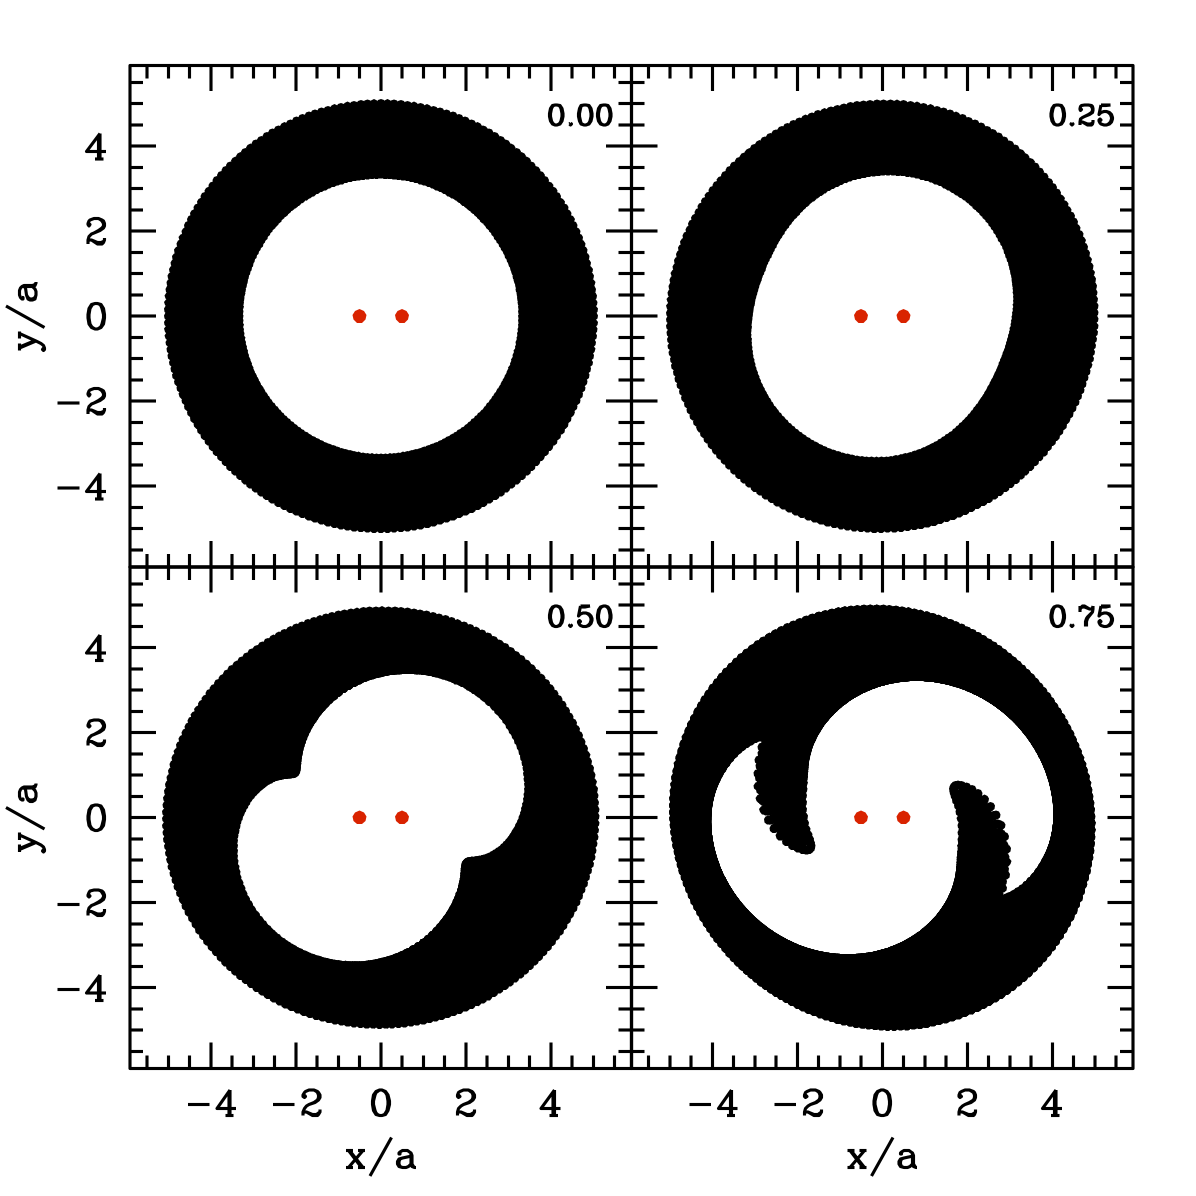
\includegraphics[scale=0.42]{figures//ch1//binary4.png} 
\caption{The distortion of a disc of massless test particles,
  initially in circular orbits around the center-of-mass of an
  equal-mass binary, with a central cavity.  The panels show snapshots
  of the locations of the disc particles after 0.25, 0.5, and 0.75
  binary orbits, as labeled.  The orbits of the particles were
  followed by solving the restricted three-body problem, and are shown
  in a frame co-rotating with the binary. The binary point masses are
  marked by the two [red] dots at $x=\pm 0.5a$.  The figure
  illustrates the tendency of the binary to create streams of
  particles entering the central cavity, due to gravity alone.}
\label{toydisc}
\end{center}
\end{figure}

Before showing the results from our simulations, we consider a simple
toy model, based on the orbits of non-interacting massless test
particles around a binary.  We populate a 2D disc with test particles,
centered on the binary's center of mass, and leave a central
cavity. We assign initial velocities equal to the Keplerian velocities
around a single point mass $M=M_p+M_s$.  We then follow the orbit of
each test particle in the rotating binary potential, by numerically
solving the restricted three-body problem for each individual particle
(for $10^5$ particles in practice, using equations 3.16 and 3.17 in
\citealt{MDbook}).

The results of this simple exercise are displayed in
Figure~\ref{toydisc}, which shows the locus of the test particles
initially, as well as after 0.25, 0.5, and 0.75 binary orbits (in a
frame co-rotating with the binary).  As this figure demonstrates,
there is a tendency for the binary to pull streams of particles into
the cavity.  This, of course, is purely a gravitational effect. As \citealt{ArtyLubow:1996} 
have pointed out, such mass flows occur near unstable 
co-rotatation equilibrium points in the binary potential. 

The toy-model can not be pushed much further in time, since after $\sim
0.75$ binary orbits, the trajectories of the test-particles cross --
this necessitates a hydrodynamical treatment.  Nevertheless, the
figure does suggest that an empty cavity can not be maintained by an
equal-mass binary, even in the absence of pressure or viscosity.
Furthermore, as we will see below, the simulations show accretion
streams with morphologies quite similar to those in the bottom right
panel of Figure~\ref{toydisc}.



\subsubsection{Hydrodynamical Evolution: Reaching Steady State}
\label{Hydrodynamical Evolution: Reaching Steady State}

We next present the results from our equal-mass binary
simulations. The disc evolves through two distinct stages.  As
explained above, the disc is set up to be out-of-equilibrium, and we
observe an initial transient state, which lasts for $\sim2500$ orbits.
We expect the details of this state to depend on the initial
conditions. The disc then settles to a quasi-steady-state, which
persists for the rest of the simulation.  In this quasi-steady-state,
the disc exhibits significant accretion, which varies periodically on
two timescales, $(1/2)t_{\rm{bin}}$ and $\sim (5 - 6)t_{\rm{bin}}$. We expect
these latter features to be robust and insensitive to initial
conditions.

{\em Transient State.}  Initially, pressure forces and viscous
stresses act to move material inside of the initial density peak at
$r\sim 8a$ inward while pressure gradients move material outside of
the density peak outward.  Once the inner disc material reaches
$r\simeq 2a$, its surface density becomes strongly perturbed and
highly non-axisymmetric.  Reminiscent of the evolution of the toy
model in \S \ref{A Toy Model}, two narrow point-symmetric streams
develop, in which the gas flow becomes nearly radial.  About 3$\%$ of
the material in these streams exits the integration domain at
$r_{\rm{min}}=a$. The rest gains angular momentum from the faster
moving black holes and is flung back toward the bulk of the disc
material at $r\simeq 2a$.  This process maintains a central cavity
within the disc, with gas streams being pulled in and pushed out on a
period of $\sim1.5 \hbox{ } \Omega_{\rm{bin}}$. 


As more disc matter flows in from the initial density peak to the
inner $r\sim 2a$ region, the streams become more dense. When these
streams are flung back out and hit the opposing cavity wall, they
generate noticeable over-densities, and deform the circular shape of
the cavity to become eccentric, though still point-symmetric.  These over-densities then
rotate at the disc's orbital velocity.  They spread out and propagate
into the disc as differential rotation causes them to wind up,
creating a point-symmetric ($m=2$), rotating spiral pattern.

  
%%%DD: NEW STREAM INTERP HERE 
{\em Quasi-Steady State.}  After the initial $\sim2500$ orbits, 
the point symmetry of the transient state breaks down as stream generation
becomes preferentially stronger on one side of the cavity. This causes 
more mass, in the form of a stream, to be driven into the opposite cavity wall, 
pushing that side of the wall farther away from the binary.  


This lopsided state can grow from a small initial asymmetry, through
a genuine physical instability, as follows:

Initially, in the transient point-symmetric state, the central cavity
has an elliptical (but still point-symmetric) shape, which rotates
along with the disc, its inner edge completing a rotation once every 3 binary
orbits. Streams are simultaneously pulled in from the two near sides
of this elliptical cavity. After the streams form, they are flung
across the cavity, and hit the region approximately diagonally across,
close to the azimuth where the opposite stream formed.  The above
process makes the cavity more eccentric over time, since when the
outward-going stream material hits the cavity wall, it pushes it
outward, further away from the binary's center of mass.

Figure \ref{Fig:AssymForm} shows the above, via three snapshots of the disc
in the transient, point-symmetric state, in time order from left to
right.  The first panel shows the initial formation of the two
opposing streams, demonstrating that the streams originate at
locations where the cavity wall is closest to the binary's center of
mass. The third panel shows the collision of the outward-going streams
with the opposing cavity wall, demonstrating that the streams collide
with the cavity wall approximately diagonally across their initiation
point.  The second panel shows the morphology of the streams half-way
between these time steps, for the sake of completeness.


\begin{figure*}
\begin{center}
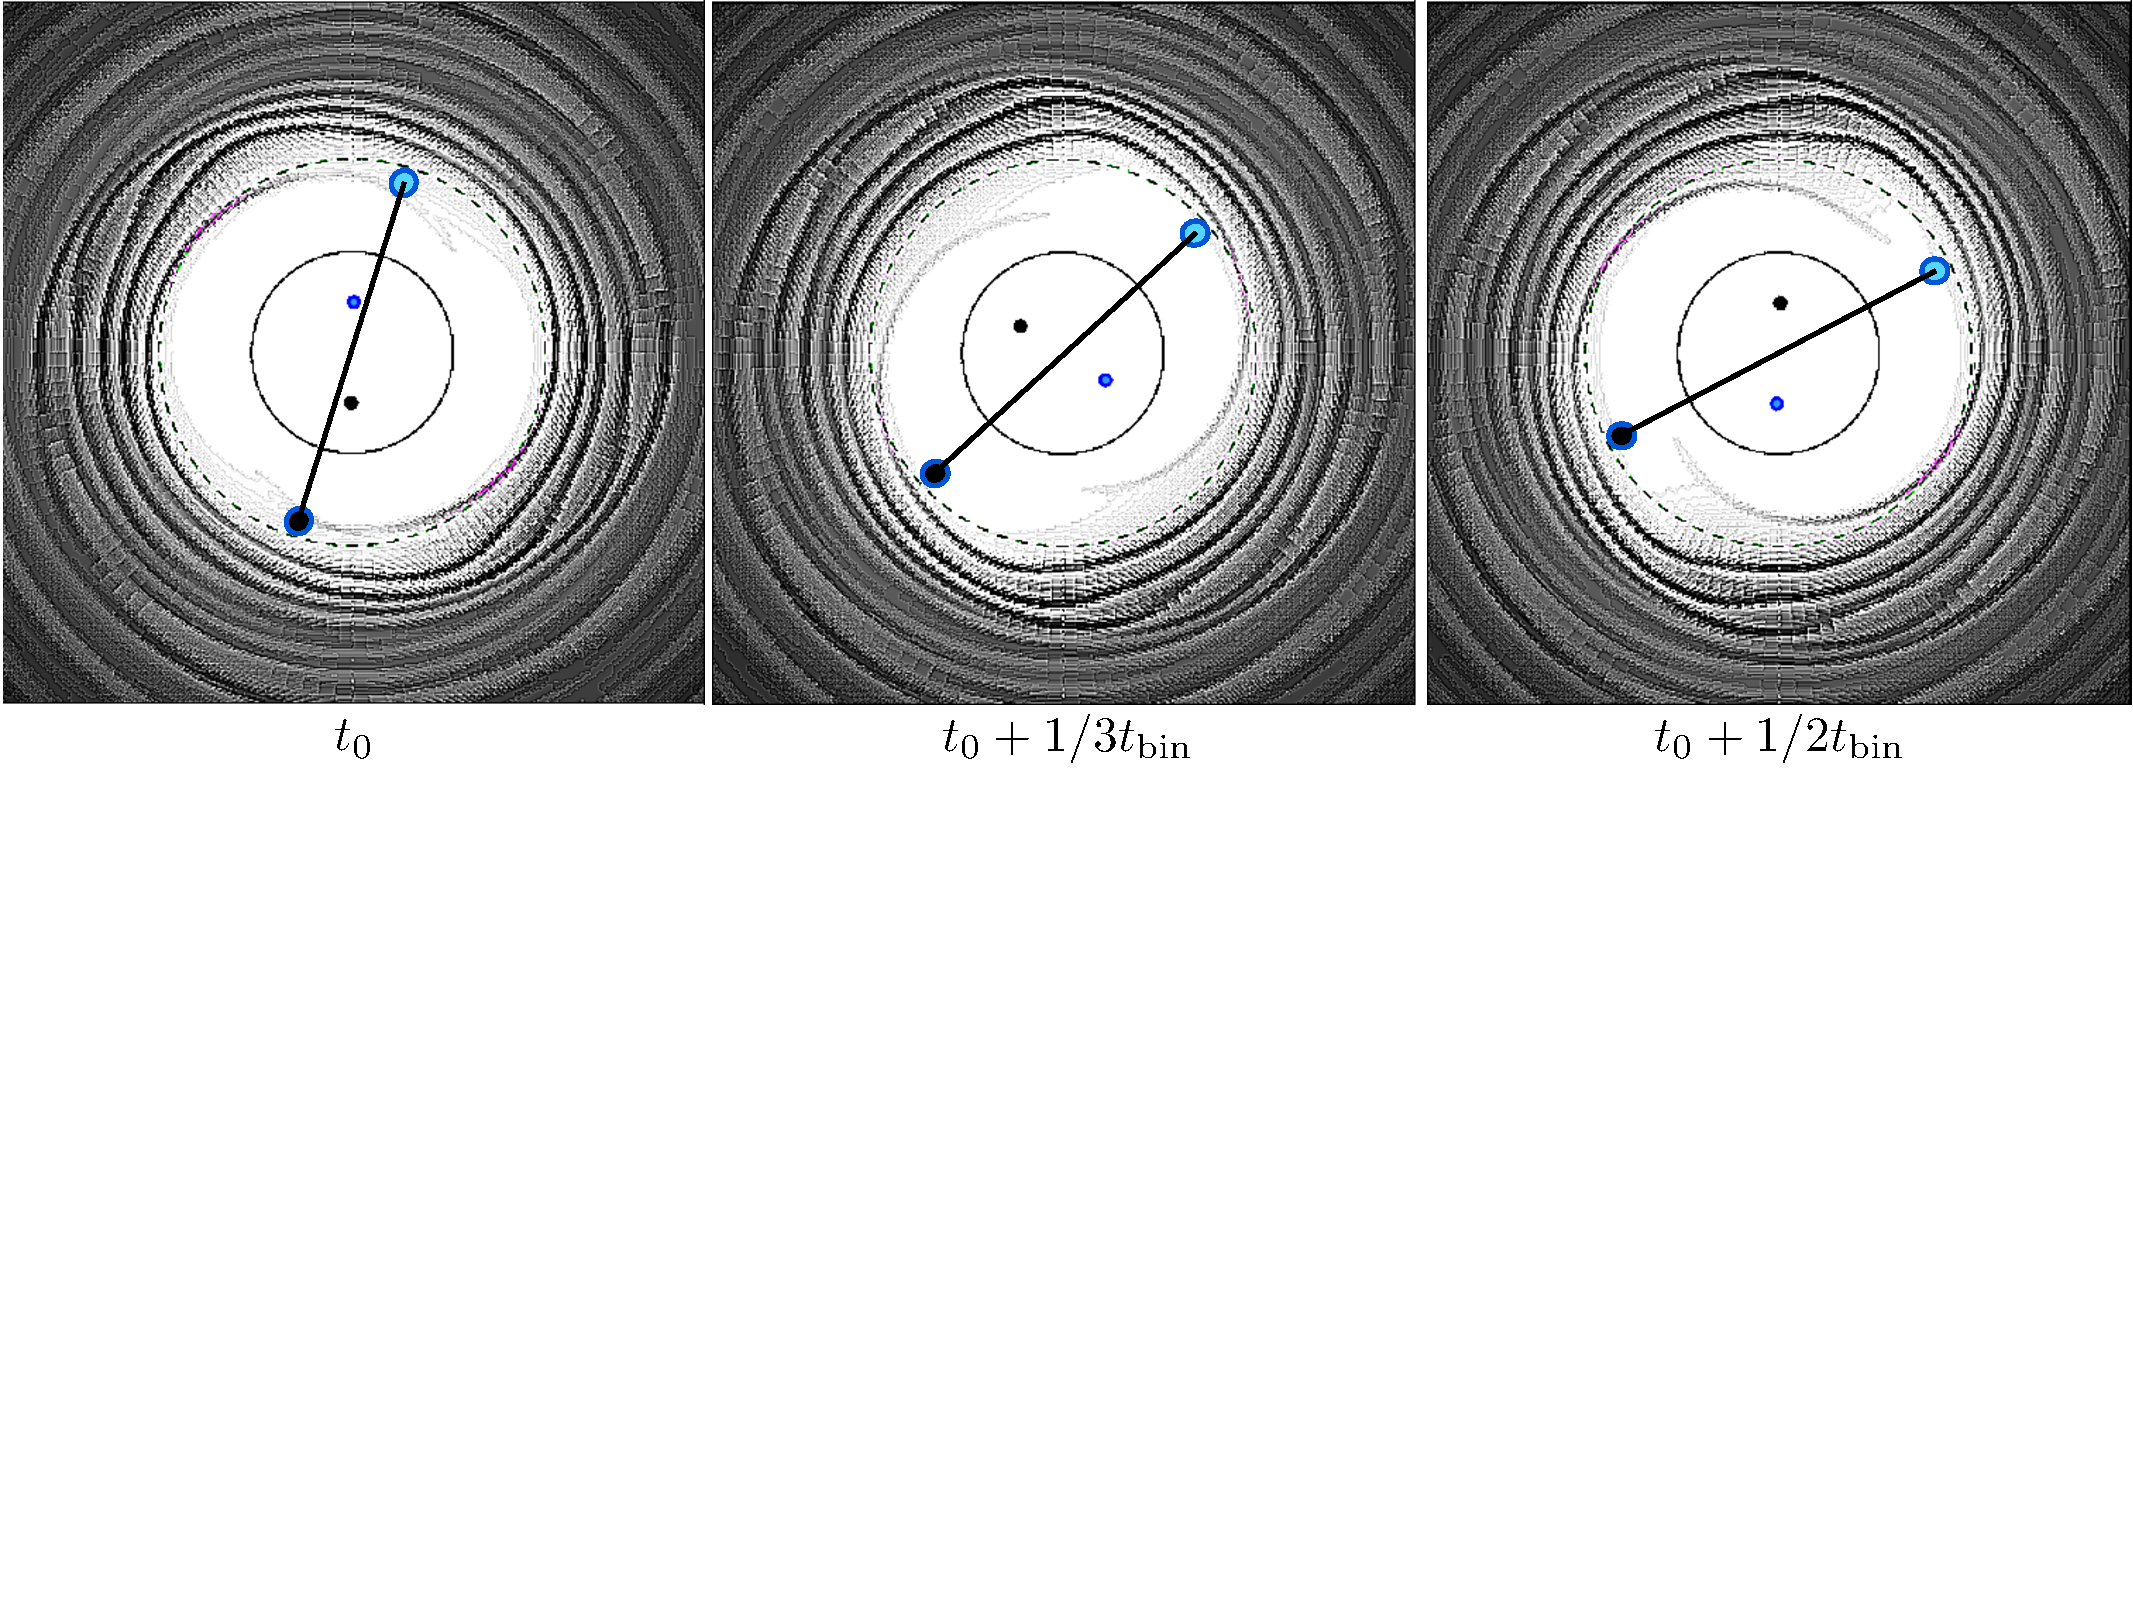
\includegraphics[scale=0.4]{figures/ch1/Stream_AsymmMode_3panel.pdf} 
\caption{Snapshots of the surface density for the $q=1$ disc in the
   point-symmetric transient state after $\sim 1350$ binary orbits. The
   snapshots are sharpened (masked to include only high Fourier
   frequencies in the image) in order to see the streams more
   clearly. The connected outer circles are drawn to guide the eye. These
   circles rotate with the disc structure at a period of $\approx 3
   t_{\rm bin}$. Streams are generated on either side of the cavity,
   (shown in the left panel; the streams shown in this panel are moving
   inward, away from the cavity wall).  These streams ultimately crash
   into the cavity wall on the diagonally opposite sides of the cavity,
   near the site where the opposing stream was generated (shown in the
   right panel; the streams shown in this panel are moving outward,
   toward the cavity wall).  If a small asymmetry causes one stream to
   become stronger, then a runaway process would ensue pushing one side
   of the disc further from the binary and allowing the other side to
   come closer; this process could ultimately be responsible for the
   observed lopsided shape of the cavity.}
\label{Fig:AssymForm}
\end{center}
\end{figure*}


Next, imagine that due to numerical noise, one stream (say, from side
"A" of the cavity) carries slightly more momentum than the spatially
opposite stream emanating from side "B".  This can happen due to a
small initial lopsidedness in the shape of the cavity, with side "A"
being closer to the binary than side "B" (or due to an asymmetry in
the density or velocity field).  In our simulations, this can only be
due to small numerical noise, but in reality, discs will obviously not
be perfectly symmetric, either.  The stronger stream will hit side "B"
of the cavity as before, but will push the cavity wall farther away
from the binary than the comparatively smaller counterpart stream
hitting side "A".  It is easy to see that this can lead to a runaway
behavior: side "A" of the cavity will have absorbed less momentum, and
will now be even closer to the binary's center of mass, relative to
side "B" - causing a larger asymmetry in the next pair of streams,
which further increases the lopsidedness of the cavity, and so on

%%%%%%%%%%%%%%%%%%%%%%%%%%%%%%%%%%%



This reenforcement-feedback process continues for a period of $\gsim$ 200-300 orbits, after
which the weaker stream, and its effect on the cavity wall structure
disappears entirely. The central cavity takes on a lopsided
shape, with a near-side where streams are pulled from the cavity wall
by each passage of the holes, and a far side where non-accreted
material from the streams is flung back and crashes into the cavity
wall.  At the azimuthal locations of these crashes, the far-side of
the wall develops very strong shocks, with Mach numbers up to
$\mathcal{M}\sim15$. (However, since our disc is locally
isothermal, this is likely an upper limit for the shock strength). 
The lopsided cavity precesses in the frame at rest with respect 
to the binary center of mass, completing a rotation once every 
$\sim400$ binary orbits. Excitation of a similar lopsided cavity is observed in the 3D MHD, as well as 2D hydrodynamical, simulations of \citealt{ShiKrolik:2012}, \citealt{Noble+2012}, and MM08. \cite{ShiKrolik:2012} explore the possible generation mechanisms of this mode. They find its growth to be consistent with being caused by asymmetric stream impacts described above. 

%%%%%%%%%%%%%%%%%%%%%%%%%%%%%%%%%%%%%
%%% 2D Density Profiles
\begin{figure*}
\begin{center}$
\begin{array}{cc}
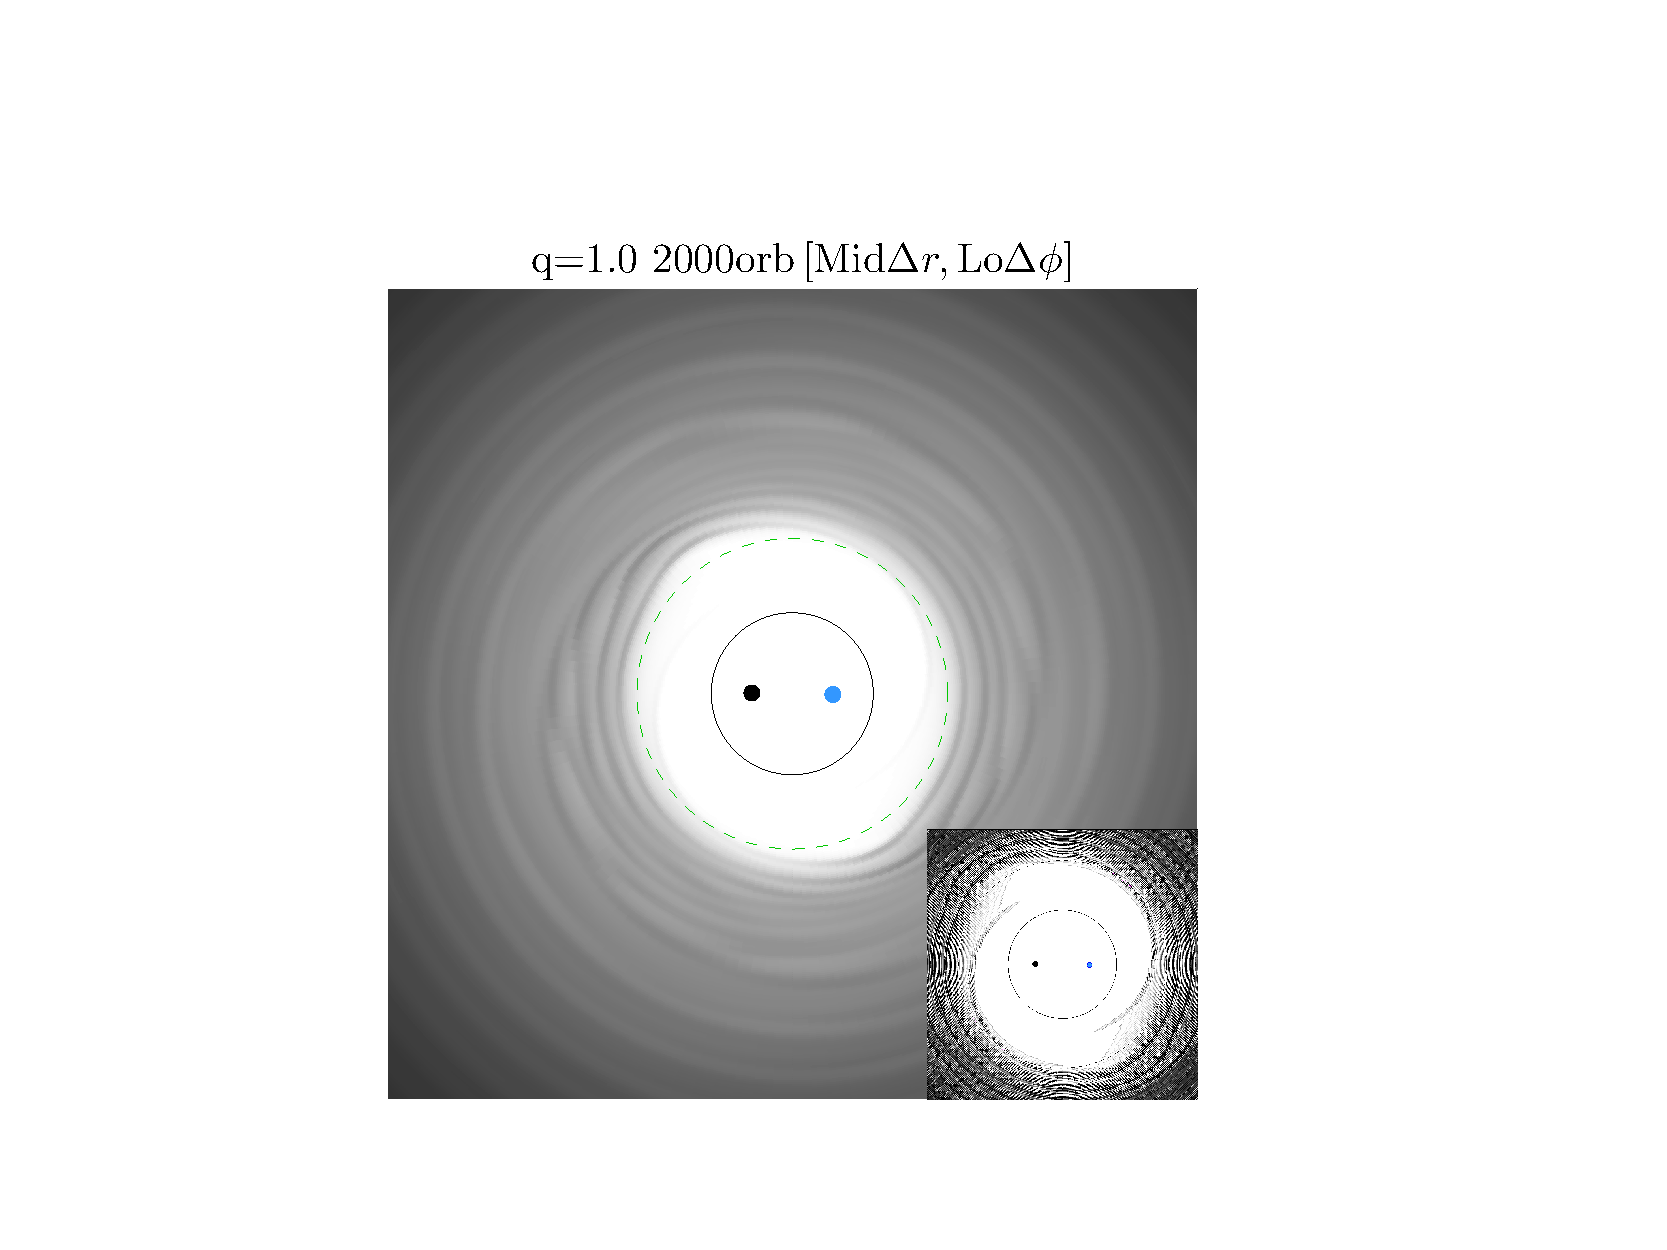
\includegraphics[scale=0.44]{figures/ch1/2DDens_q1_Danvisc_MM_a01_M1G_100a_r24y78_FIG_2000_SHARP_STREAMINSET}&
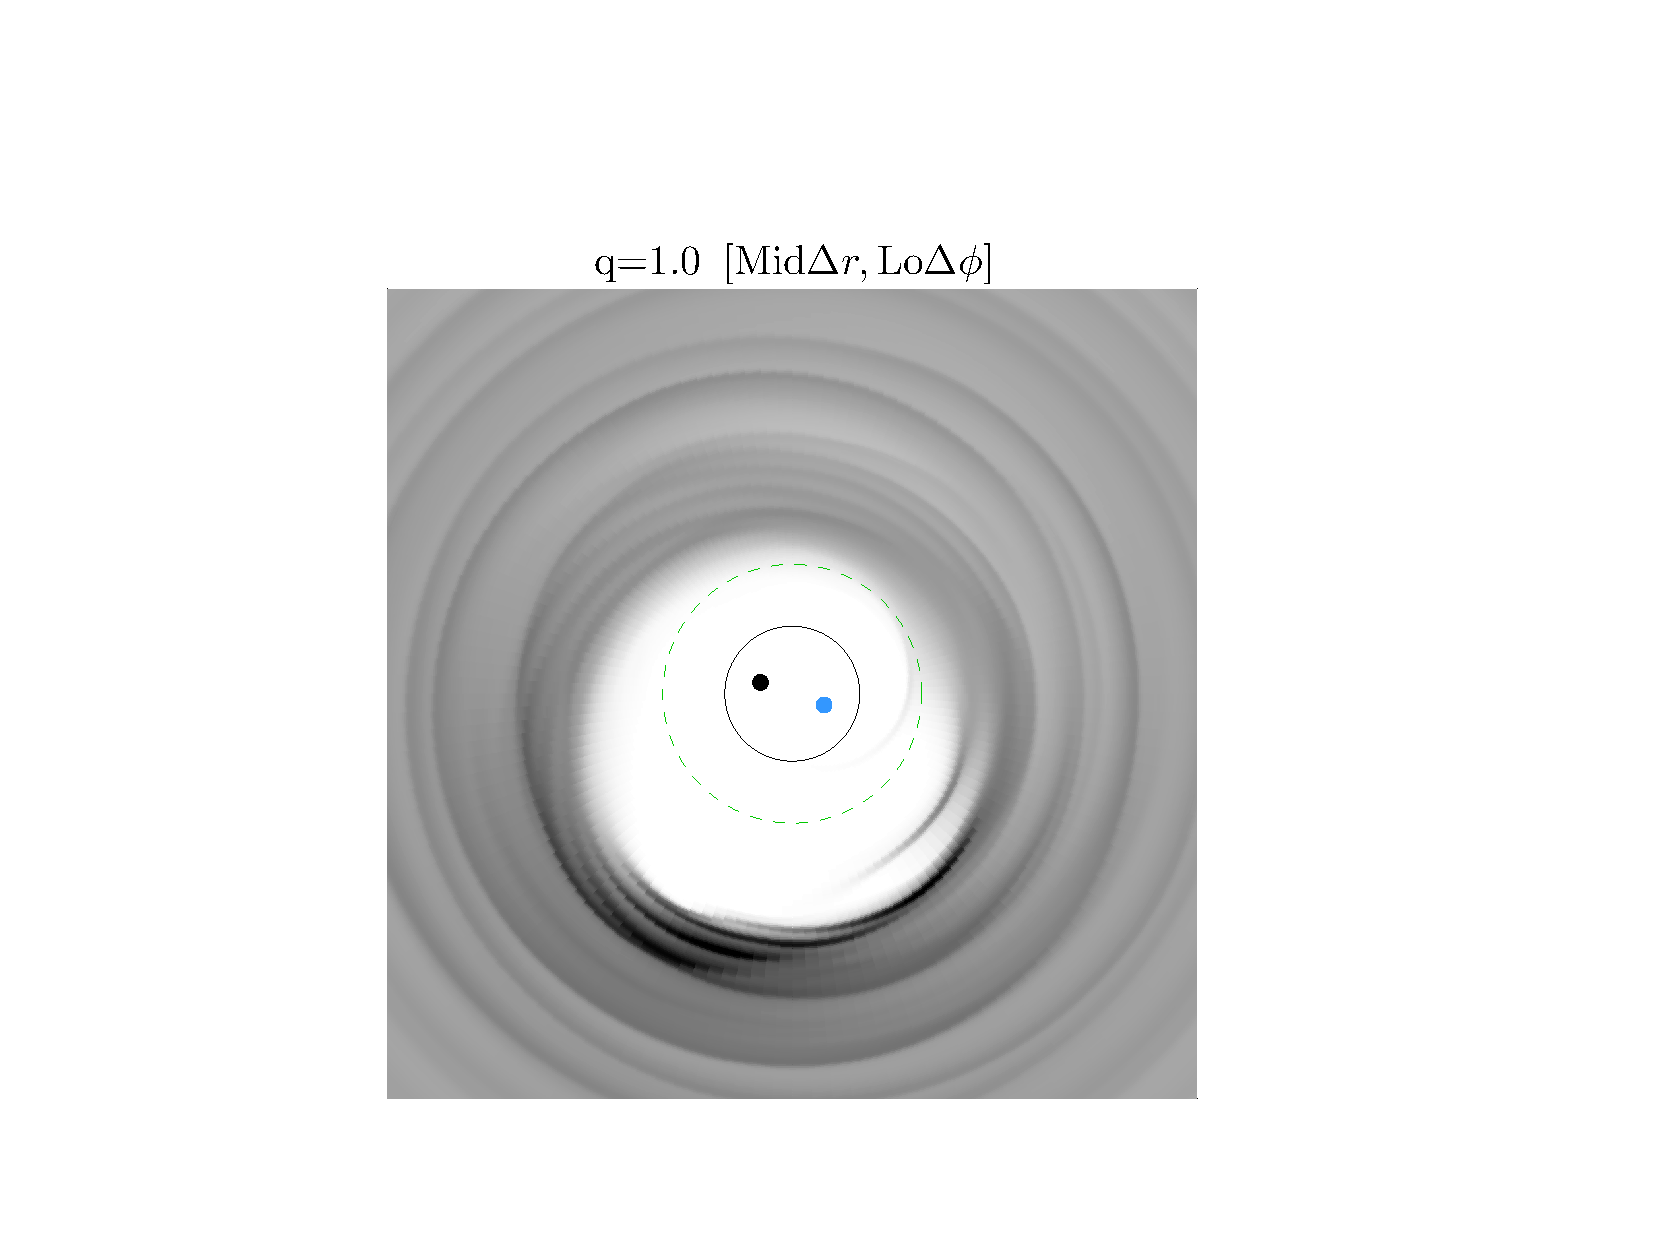
\includegraphics[scale=0.44]{figures/ch1/2DDens_q1_Danvisc_MM_a01_M1G_100a_r24y78_FIG3_4000}  \\ \\
\hline  \hline\\ 
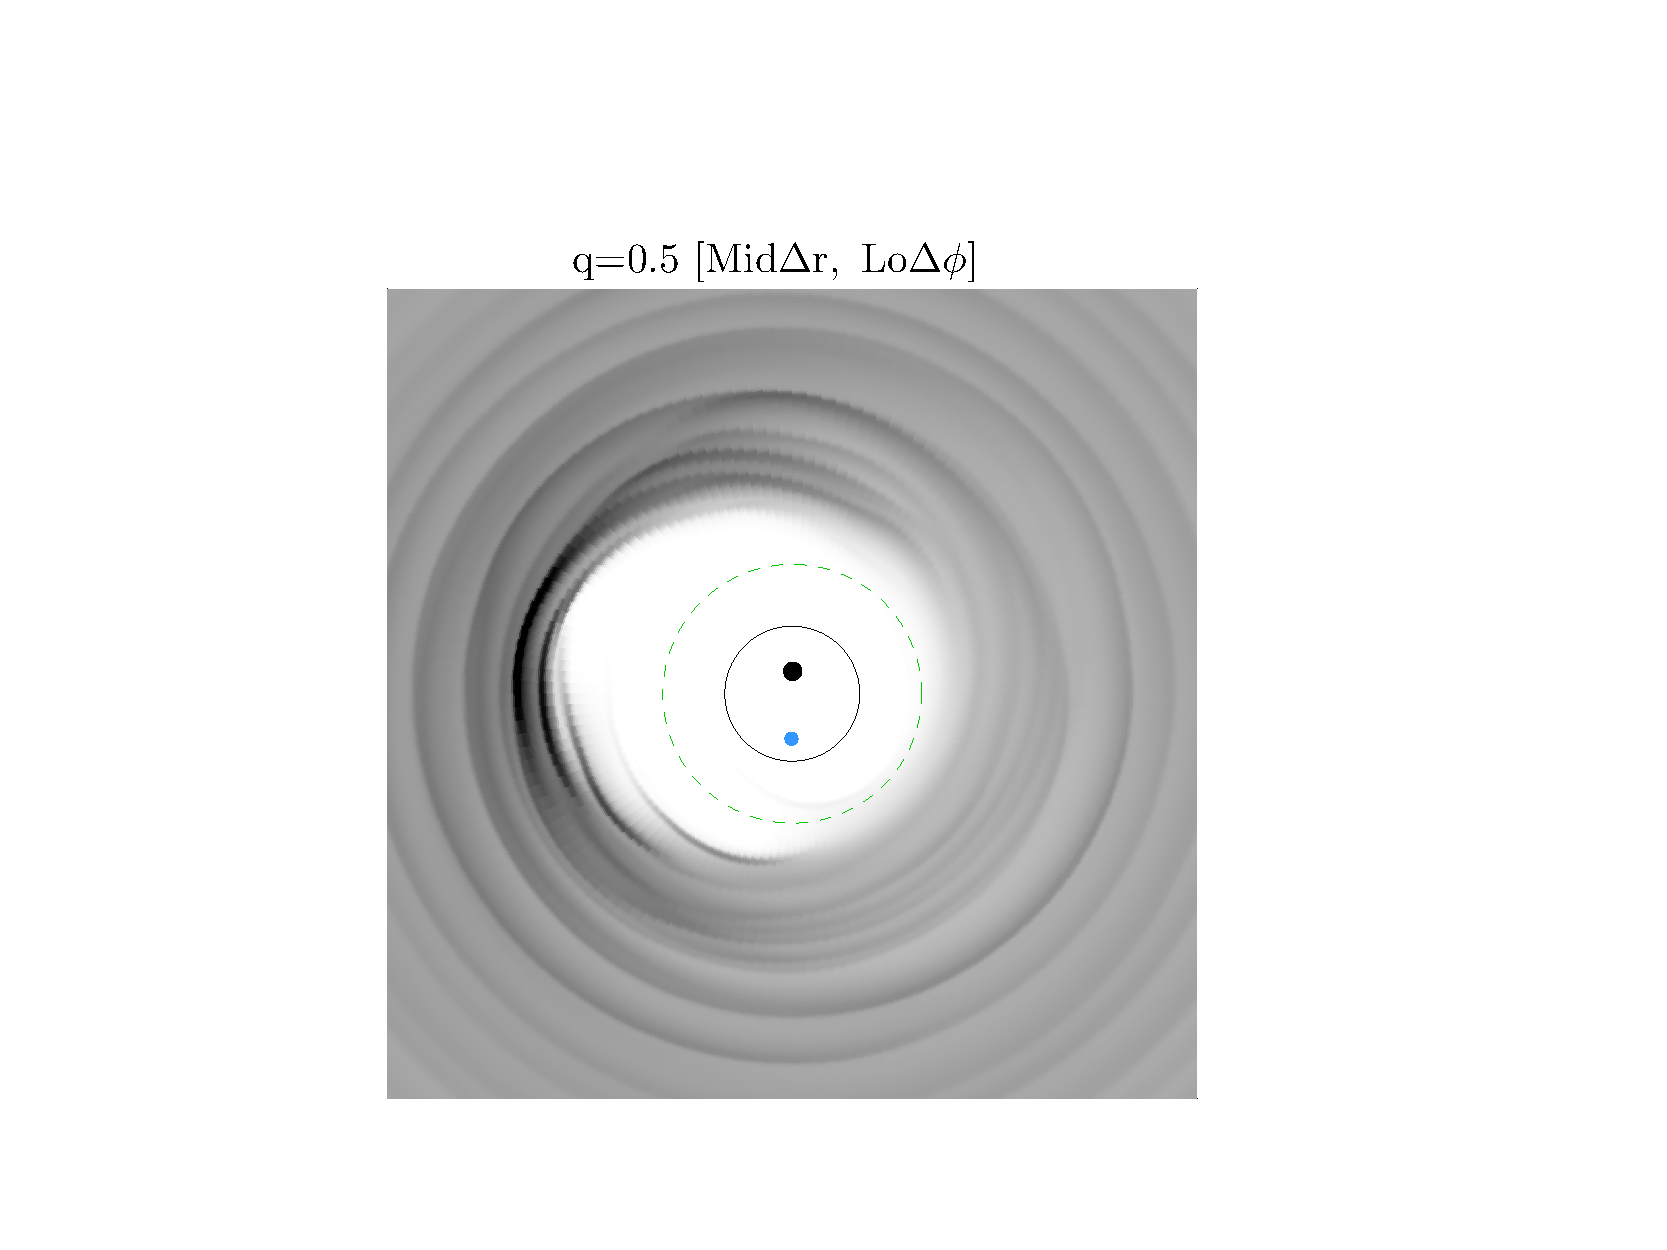
\includegraphics[scale=0.44]{figures/ch1/2DDens_q05_Danvisc_MM_a01_M1G_100a_r24y78_FIG_4004} &
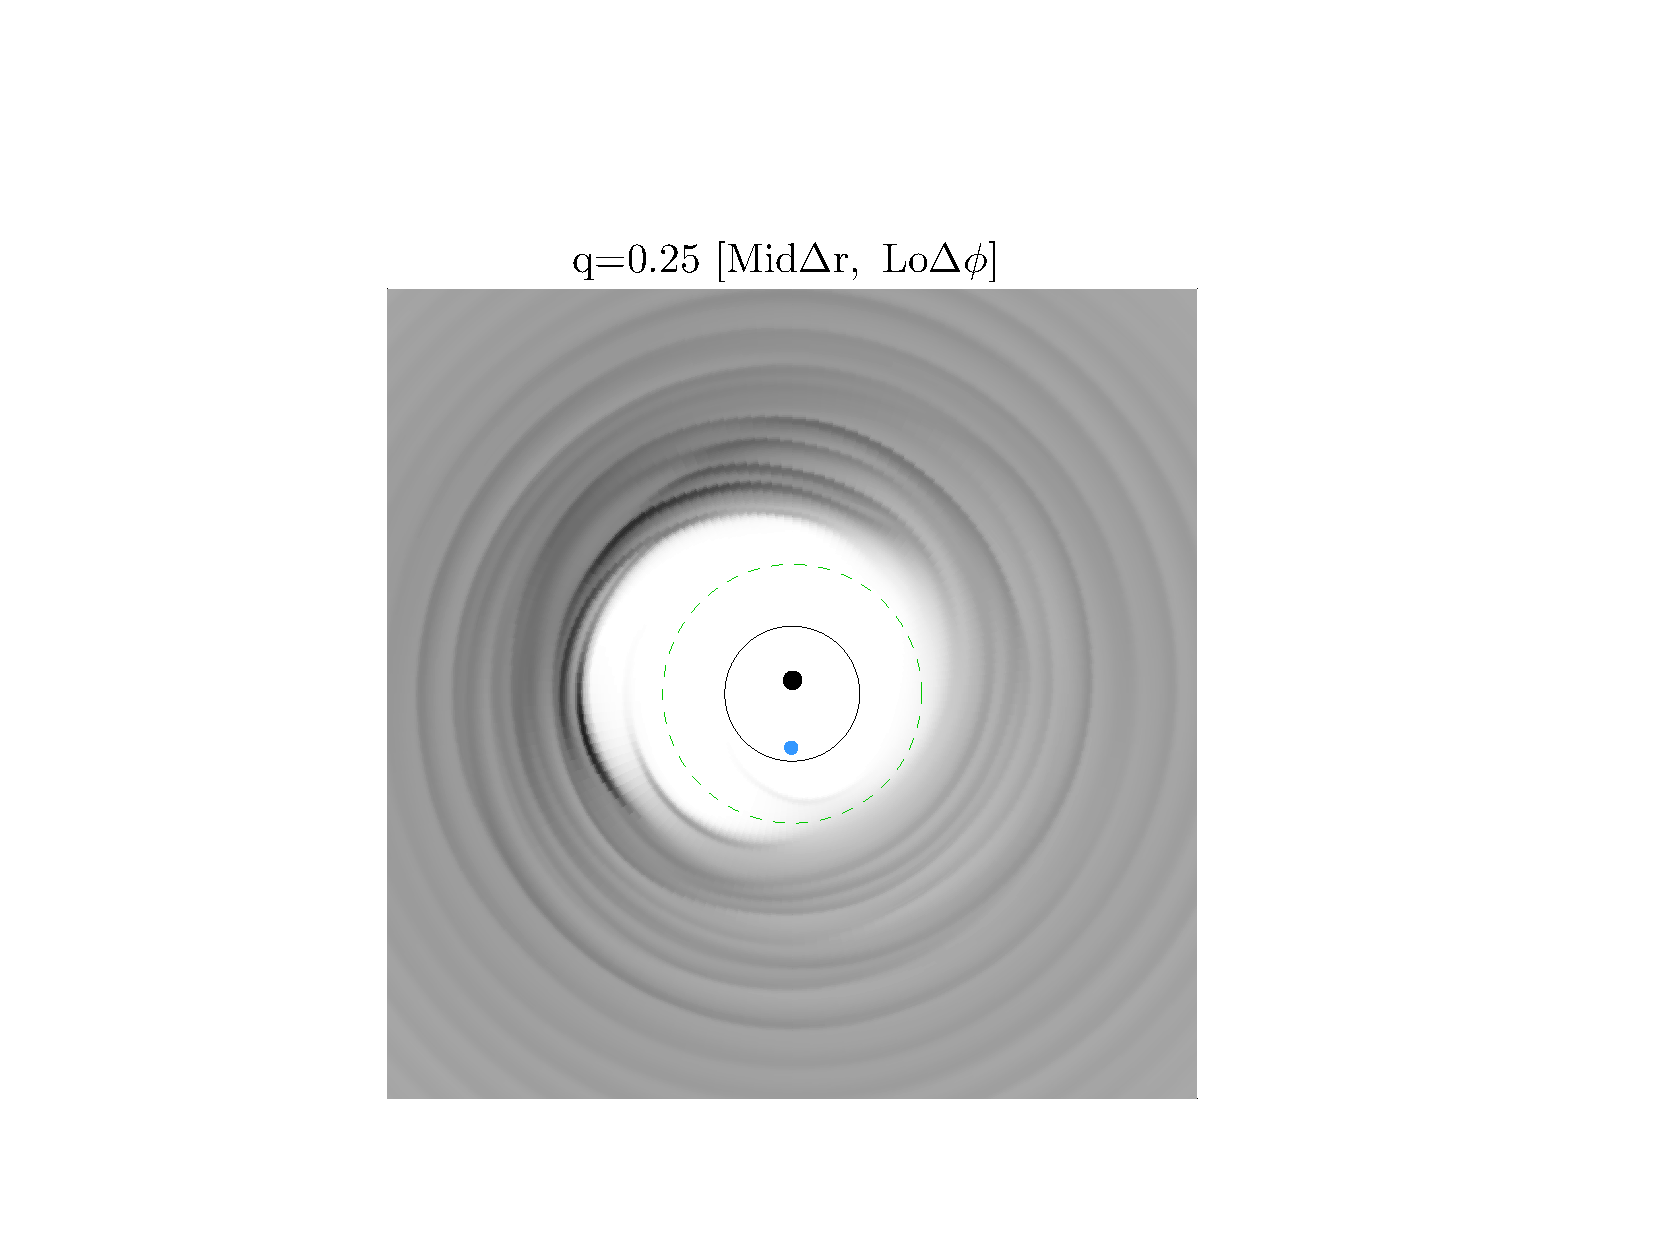
\includegraphics[scale=0.44]{figures/ch1/2DDens_q25_Danvisc_MM_a01_M1G_100a_r24y78_FIG_4004}\\
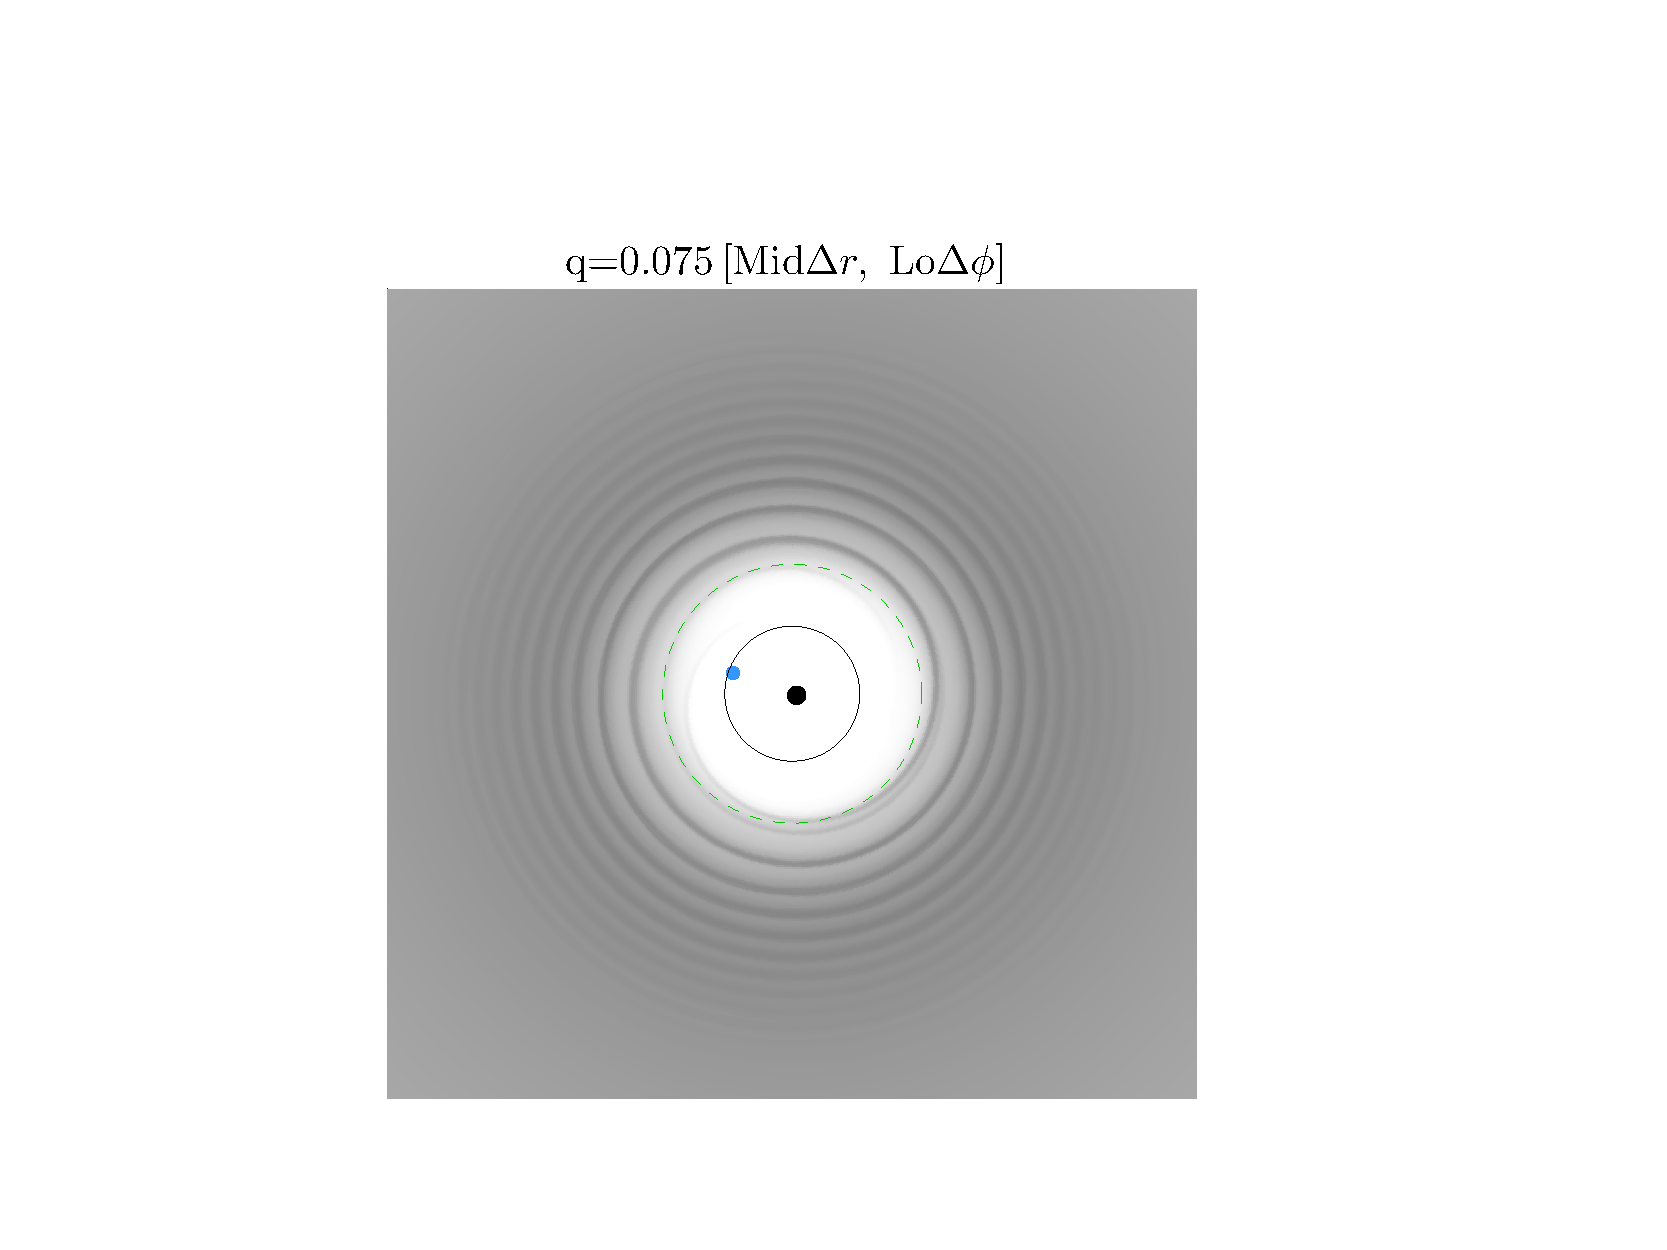
\includegraphics[scale=0.44]{figures/ch1/2DDens_q075_Danvisc_MM_a01_M1G_100a_r24y78_FIG_4010} &
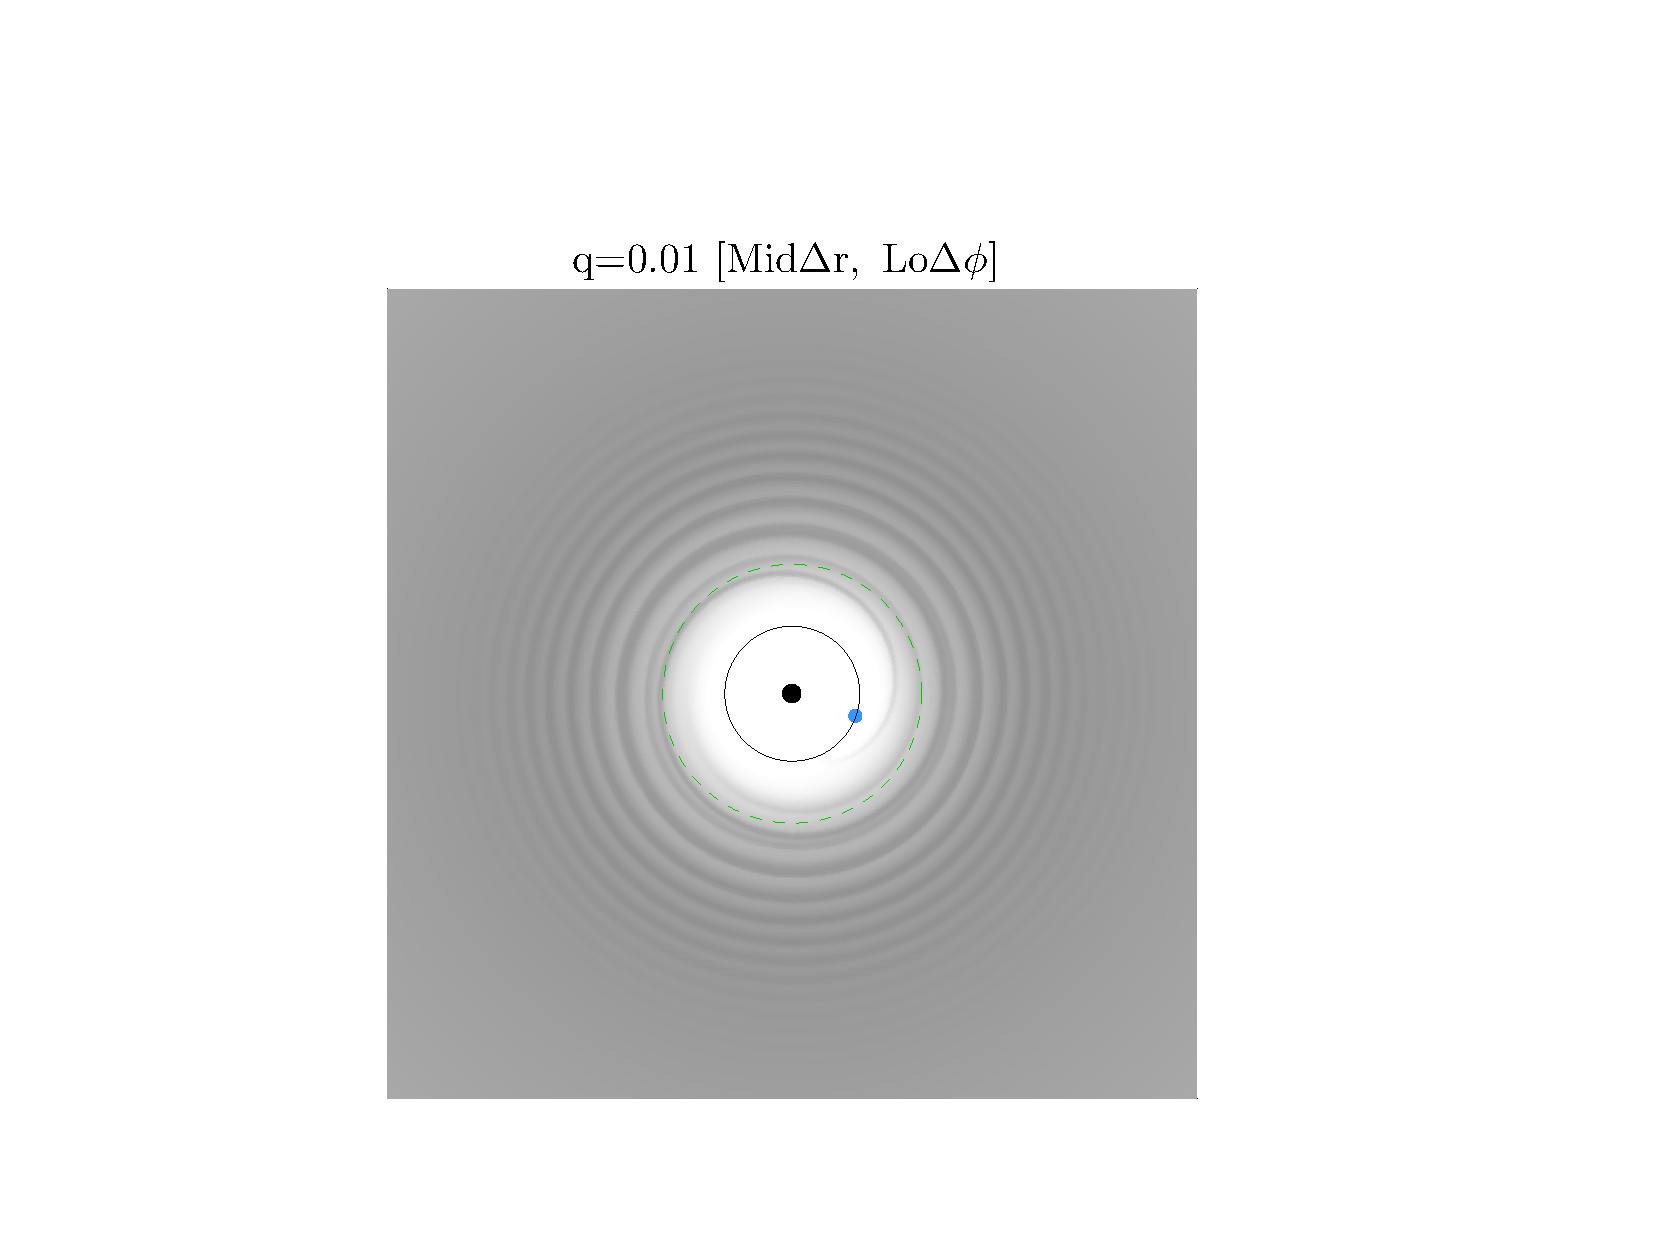
\includegraphics[scale=0.44]{figures/ch1/2DDens_q001_Danvisc_MM_a01_M1G_100a_r24y78_FIG_4000} 
\end{array}$
\end{center}
\caption{\textit{Top row:} Surface density distributions for the
  equal-mass ratio ($q=1.0$) binary during a transient,
  point-symmetric state after $\sim1000$ binary orbits (left) and
  during the quasi-steady asymmetric state after $\sim$ 4000 binary
  orbits (right). The inset in the top left panel zooms in to the
  inner $\pm 2.5 r/a$ of the disc in order
  to show the stream morphology.  \textit{Bottom two rows:} snapshots
  at $\sim$ 4000 binary orbits, during the quasi-steady-state phase,
  for mass ratios $q=0.5, 0.1, 0.075$, and $0.01$, as labeled.  Each
  panel shows the inner $\sim6\%$ of the simulated disc, extending
  $\pm 6 r/a$ in both directions.  The solid circles mark the inner
  boundary of the simulation at $r=r_{\rm{min}}=a$. The larger dotted
  circle at $r\simeq2.08a$ is the position of the $(m,l)=(2,1)$ outer
  Lindblad resonance (shown only for reference).  Surface densities
  are plotted with the same linear grayscale in each panel, with the
  darkest regions corresponding to a maximum density of $0.8 \Sigma_0$
  ($0.4 \Sigma_0$ for the top left panel). Orbital motion is in the clock-wise direction.}
\label{2DDensProf}
\end{figure*}
%%%%%%%%%%%%%%%%%%%%%%%%%%%%%%%%%%%


We show examples of the two-dimensional surface density distributions
in Figure \ref{2DDensProf}.  The top row of this figure shows
snapshots at $\sim1000$ binary orbits (left) and at $\sim$4000 binary
orbits (right), of the inner 6$\%$ of the simulated disc (i.e. $\pm 6 r/a$ are
shown in both directions).  The solid circle marks the inner boundary
of the simulation domain at $r=r_{\rm{min}}=a$.  The larger dotted
circle at $r\simeq2.08a$ is the position of the $(m,l)=(2,1)$ outer
Lindblad resonance (not present, but shown for reference).  The left of these two
panels illustrates the point-symmetric, transient state. The
zoomed-in inset of this panel shows two weak point-symmetric streams reminiscent of the streams seen in the toy
model of Figure \ref{toydisc}. The right panel shows the disc after it
has settled to its quasi-steady, lopsided state, with a single stream.


%%% AZ AVG Density
\begin{figure*}
\begin{center}$
\begin{array}{cc}
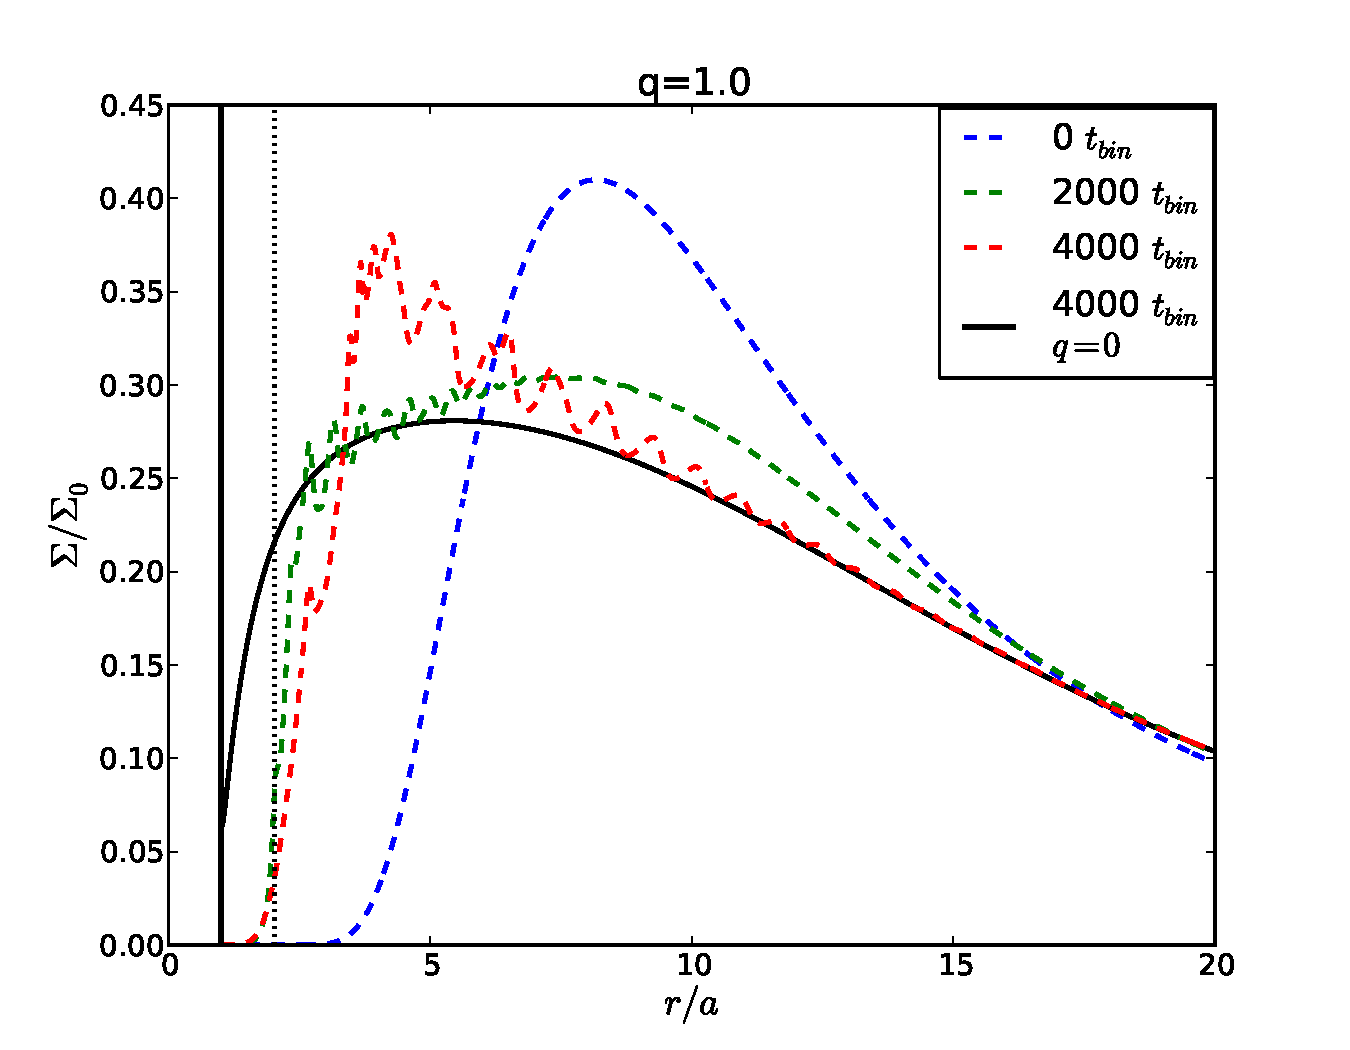
\includegraphics[scale=0.39]{figures/ch1/AzAvg_FulVsc_q1_100a_M1G_alph01_Resr024y78} &
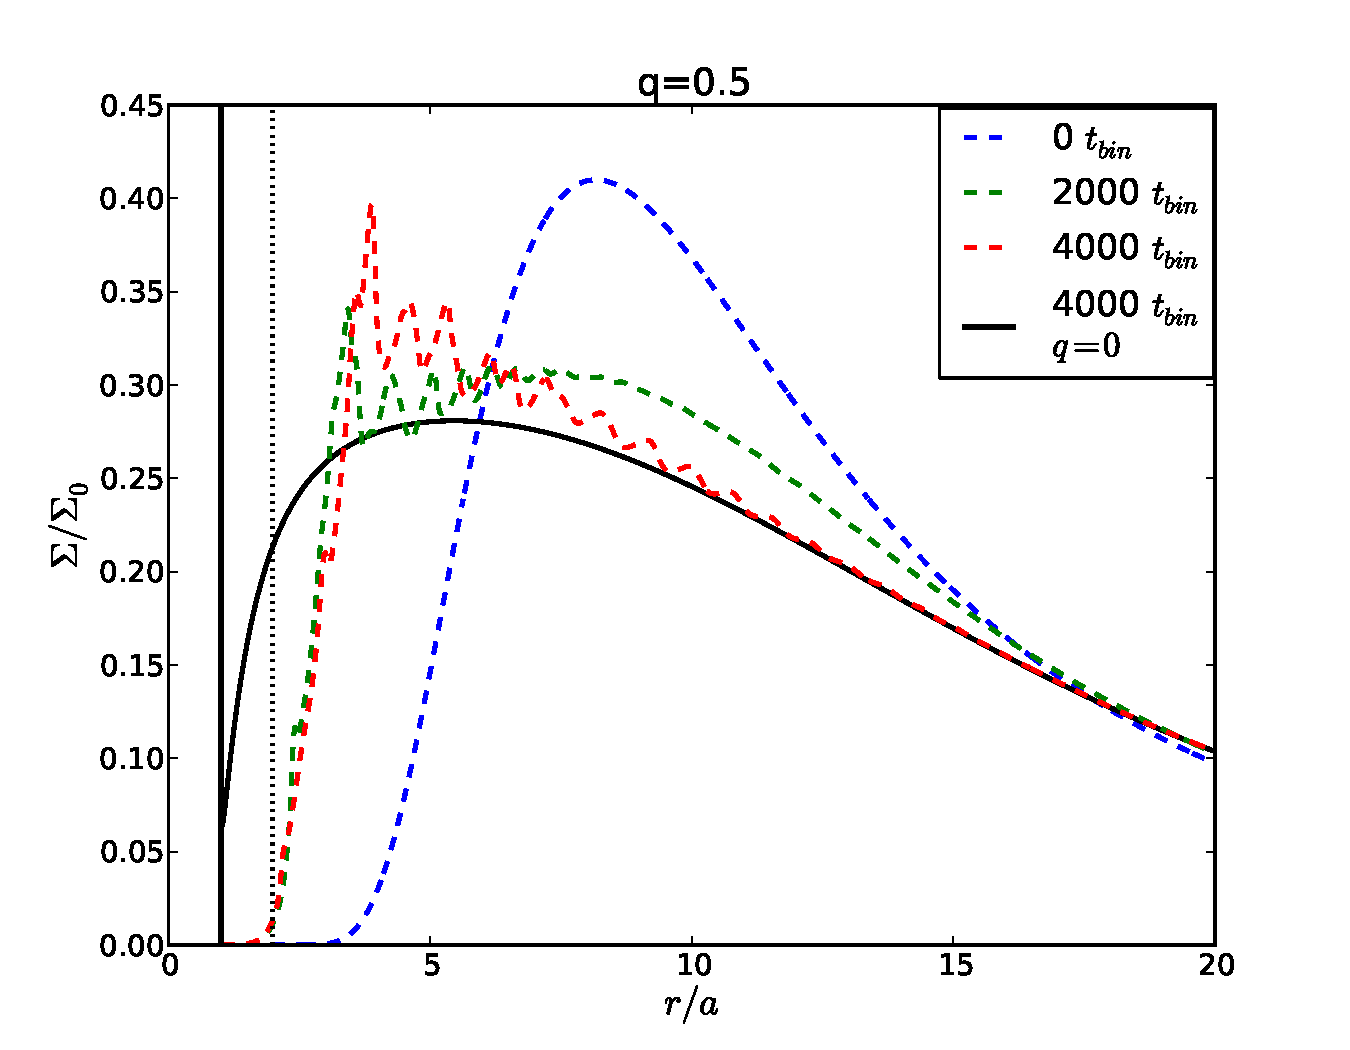
\includegraphics[scale=0.39]{figures/ch1/AzAvg_FulVsc_q05_100a_M1G_alph01_Resr024y78} \\
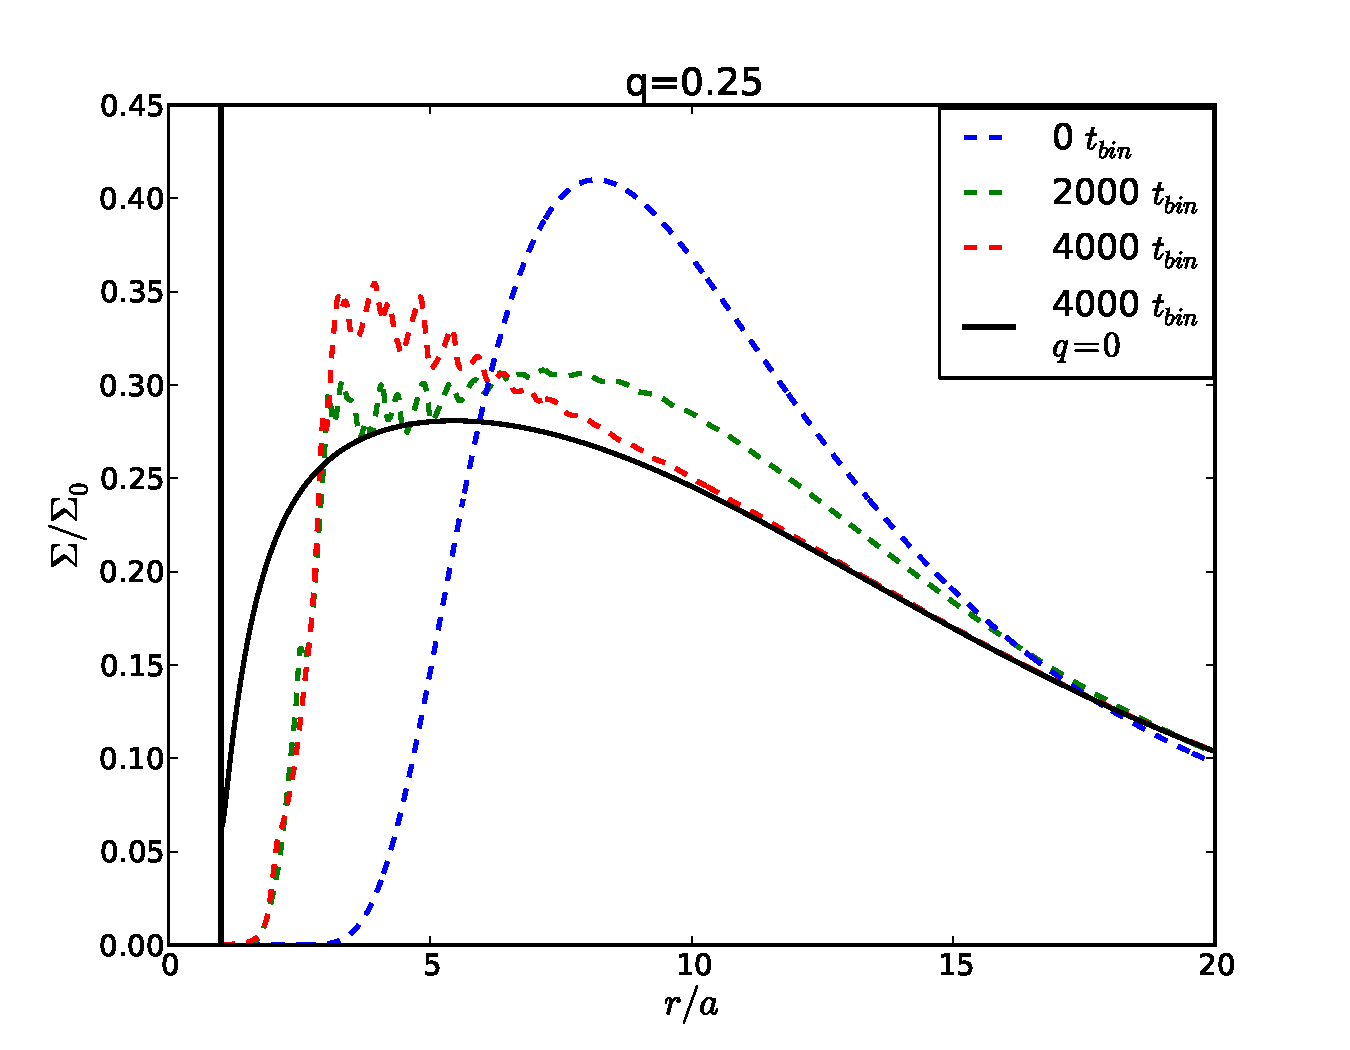
\includegraphics[scale=0.39]{figures/ch1/AzAvg_FulVsc_q25_100a_M1G_alph01_Resr024y78} &
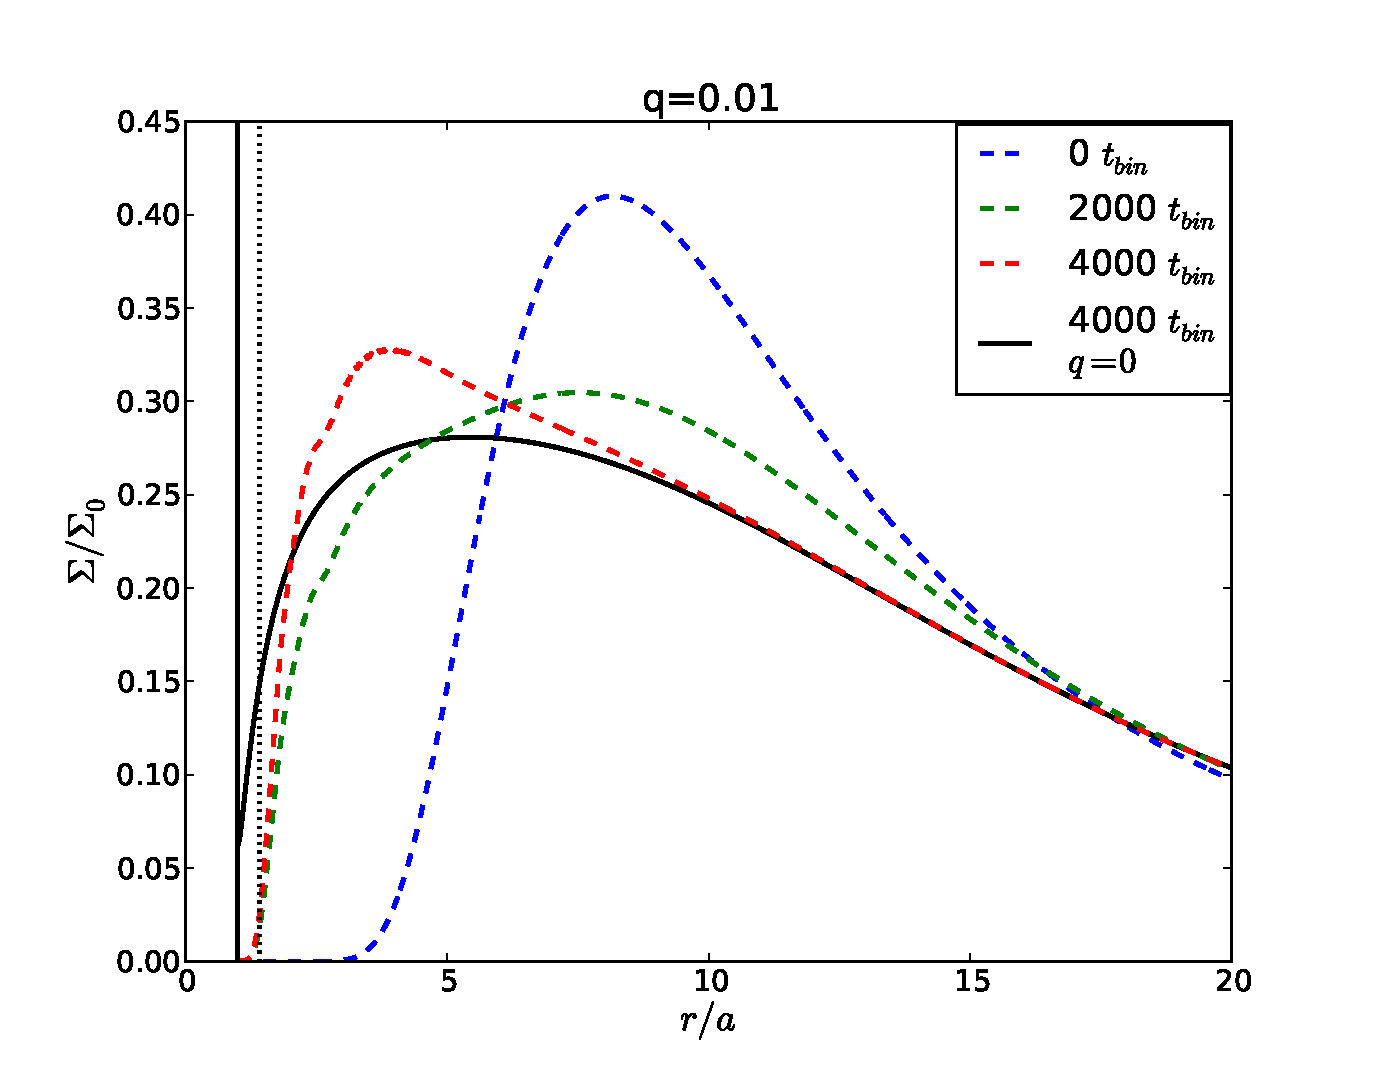
\includegraphics[scale=0.39]{figures/ch1/AzAvg_FulVsc_q001_100a_M1G_alph01_Resr024y78}   %.eps extensions 
\end{array}$
\end{center}
\caption{Snapshots of the azimuthally averaged disc surface density at
  different times (shown by different curves in each panel, from 0
  to 4000 orbits, as labeled), and for different mass ratios (shown in
  different panels, from $q=1.0$ to $0.01$, as labeled).  In each
  panel, the solid [black] curve shows, for reference, the density
  profile in the point-mass ($q=0$) case after 4000 orbits. The
  vertical dotted lines mark the radius where binary and viscous
  torques balance (from Figure \ref{TrqDq}); these lie close to the
  observed cavity edges.  The vertical solid lines mark the inner edge
  of the integration domain ($r=r_{\rm{min}}=a$).  In each case, the
  inner circumbinary disc spreads inward with time, but the density
  profile remains sharply truncated, with a low-density central cavity
  inside $r \lsim 2a$.  }
\label{AzAvDens}
\end{figure*}


The top left panel of Figure~\ref{AzAvDens} shows snapshots of the
azimuthally averaged surface density profile of the equal-mass binary
disc at three different times, after 0, 2000, and 4000 orbits. For
comparison, the density profile is also shown for the single
point--mass ($q=0$) case, after 4000 orbits.  As the figure shows, the
inner circumbinary disc spreads inward with time. By 4000 orbits, the
disc structure at $r/a\gsim 5$, where the effect of the binary is
relatively small, closely follows the $q=0$ case.  However, the
density profile remains sharply truncated inside $r \lsim 2a$
(i.e. below the point--mass case, even at 4000 orbits).  As a result of the initial density profile, the peak
density first decreases as matter drains inward towards the holes and also
outward towards the outer boundary. With time, despite the leakage of 
streams to the binary, inward viscous diffusion causes a gas 
pileup behind the cavity wall.   The figure also shows that the
position of the cavity wall moves slightly outward between the t=2000
and t=4000 snap-shots. This is because as the disc settles to its
lopsided quasi-steady-state, the cavity size grows in the azimuthally
averaged sense.



\subsubsection{Torque Balance and the Size of the Central Cavity}
\label{Torque Balance and the Size of the Central Cavity}

As (the top left panel of) Figure \ref{AzAvDens} shows, the central
cavity around the equal-mass binary extends to $r \sim 2a$.  Here
we take the cavity edge $r_{\rm{ce}}$ to be the radius where the negative 
viscous torque density matches the binary torque density (in an azimuthally averaged sense) ,
%
\begin{equation}
\left[ \left(\frac{dT}{dr}\right)_{\rm{bin}}  + \left(\frac{dT}{dr}\right)_{\rm{visc}} \right]_{r_{\rm ce}} = 0.
\label{TrqBalRCE}
\end{equation}
%
To gain insight into the transport of angular momentum and the
clearing of the central cavity, we therefore compute the time-- and
azimuthally--averaged torque densities from the binary potential,
%
\begin{equation}
\left(\frac{dT}{dr}\right)_{\rm{bin}} = \left< \frac{1}{2 \pi}  \int^{2 \pi}_{0}{ \Sigma(r, \phi) \frac{d\Phi}{d\phi}(r,\phi) r d\phi }\right>_{t},
\label{DTb_num}
\end{equation}
%
and from viscous stresses,
%
\begin{equation}
\left(\frac{dT}{dr}\right)_{\rm{visc}} = 2 \pi \left<  \frac{d}{dr}\left[ r^3 \nu \left< \Sigma \frac{\partial \Omega}{\partial r} \right>_{\phi}\right] \right>_{t}.
\label{DTv_num}
\end{equation}
%
The outer derivative in equation (\ref{DTv_num}) is taken numerically,
and all of the above values are measured directly from the simulation
outputs, except for the binary potential derivative in equation
(\ref{DTb_num}) which is given analytically. The time averages are 
taken over $25$ binary orbits at a sample rate of 20 per orbit.


%%% TORQUES %%%%%
\begin{figure*}
\begin{center}$
\begin{array}{cc}
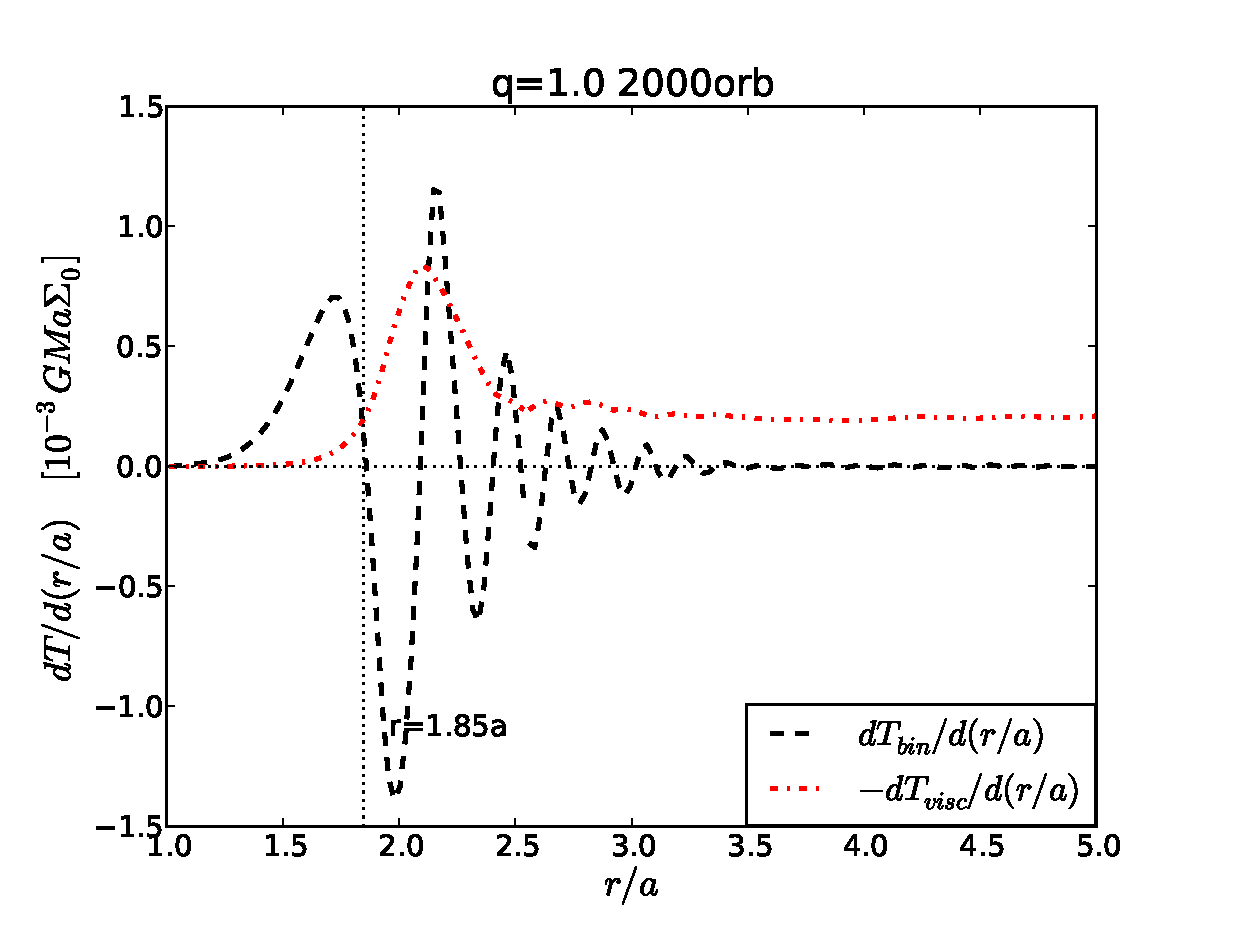
\includegraphics[scale=0.445]{figures/ch1/TRQDENS_EARLY_FulVsc_a01_q1_Resr24y78.eps} &
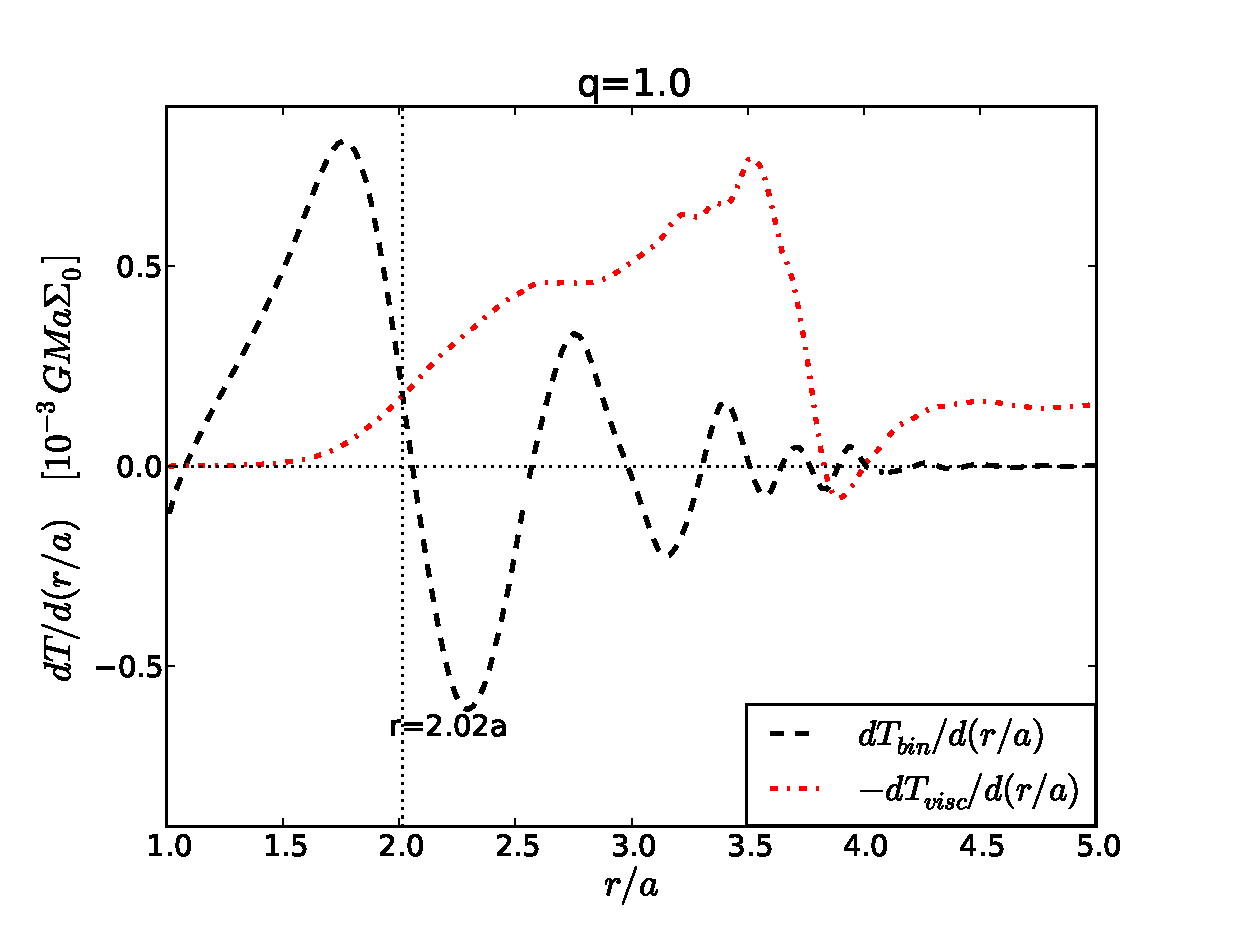
\includegraphics[scale=0.445]{figures/ch1/TRQDENS_LATE_FulVsc_a01_q1_Resr24y78.eps} \\
%
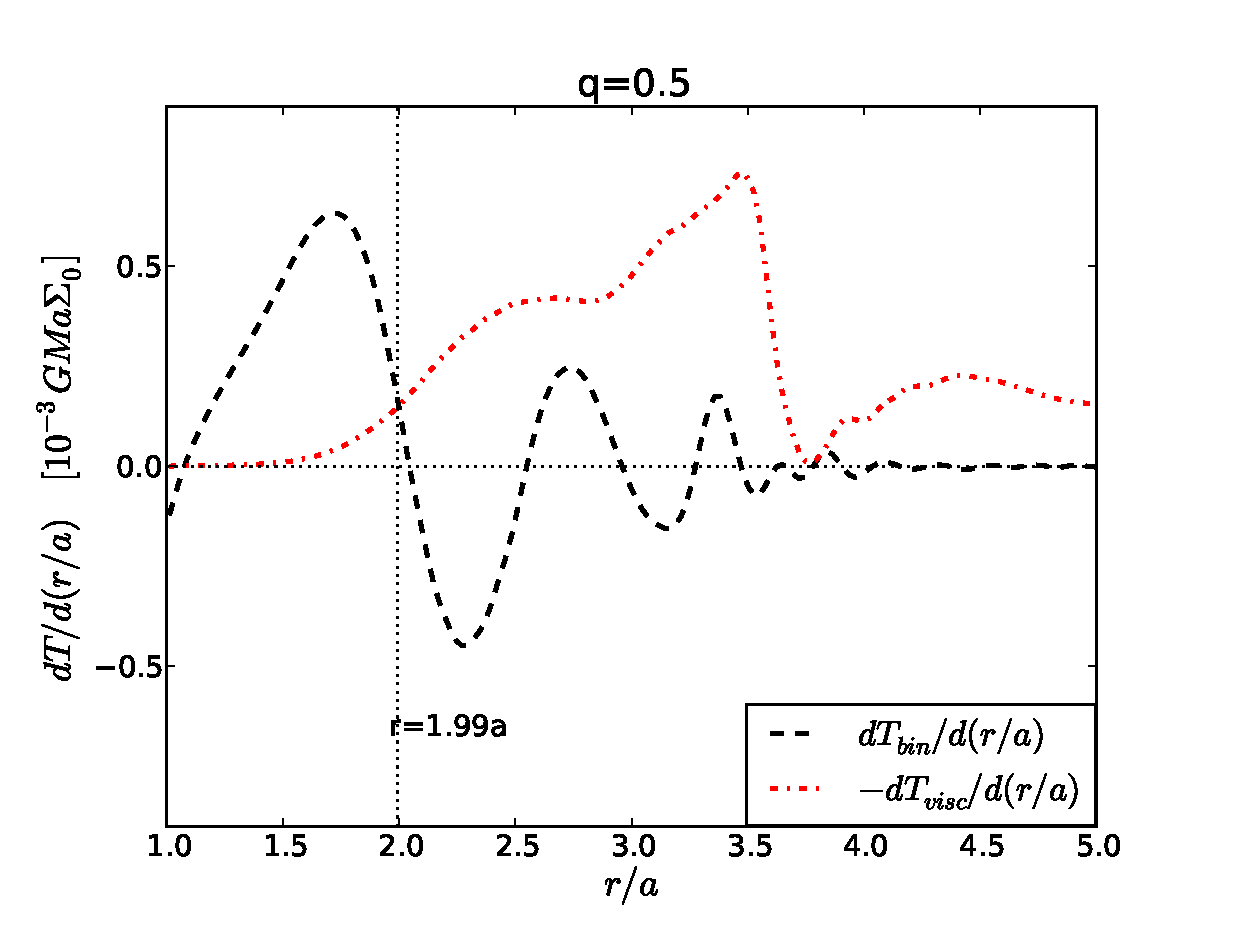
\includegraphics[scale=0.445]{figures/ch1/TRQDENS_LATE_FulVsc_a01_q05_Resr24y78.eps} &
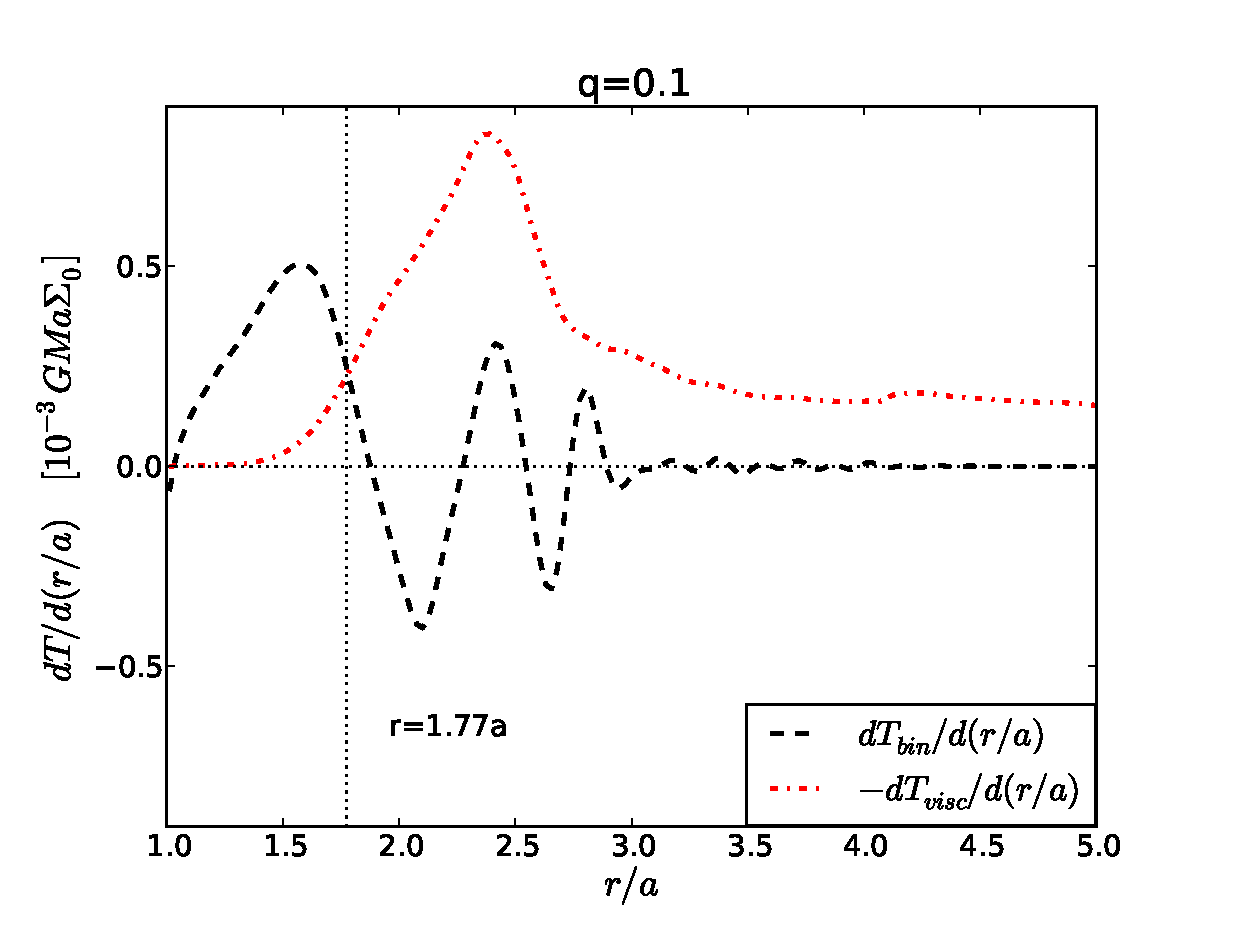
\includegraphics[scale=0.445]{figures/ch1/TRQDENS_LATE_FulVsc_a01_q01_Resr24y78.eps} \\
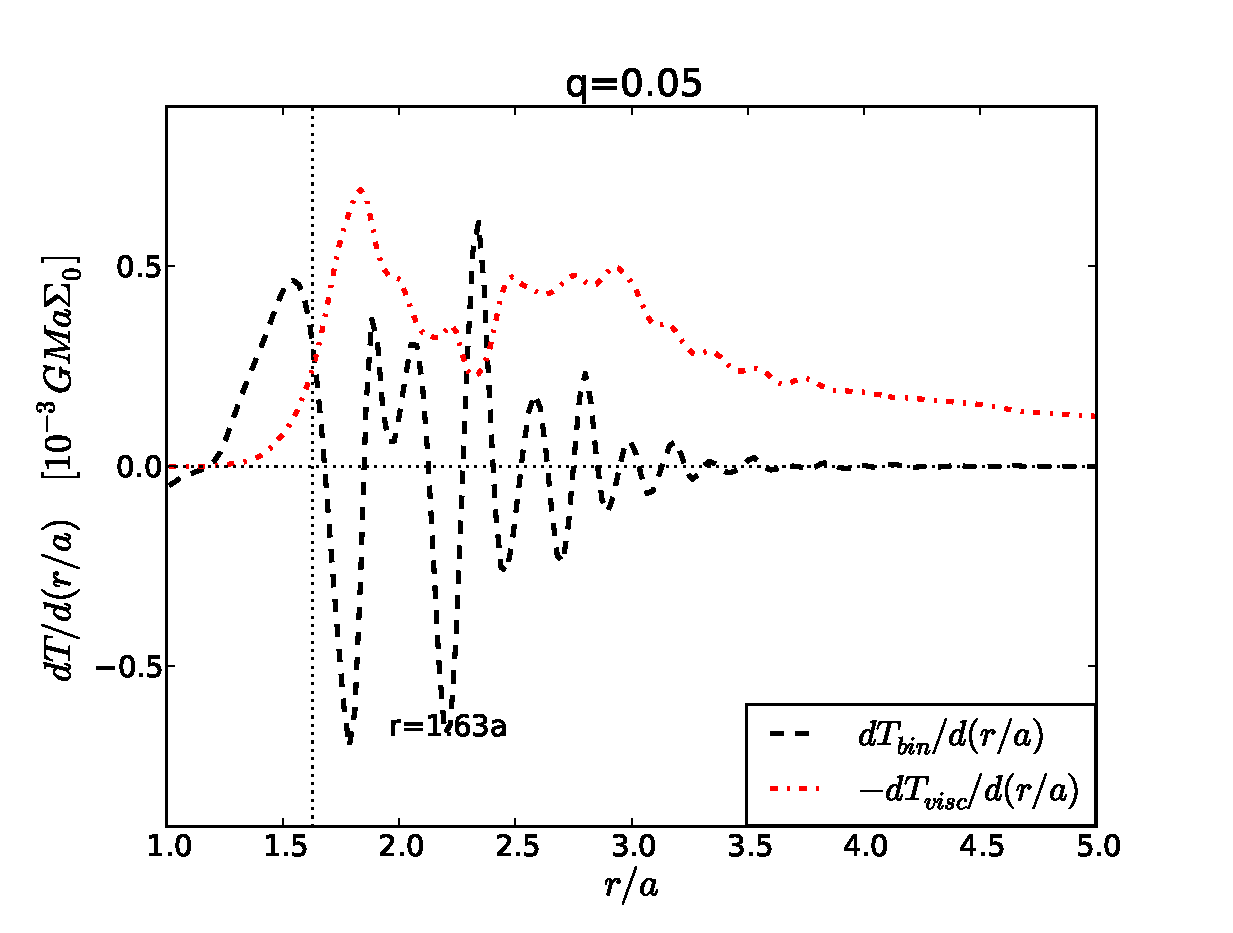
\includegraphics[scale=0.445]{figures/ch1/TRQDENS_LATE_FulVsc_a01_q005_Resr24y78.eps} &
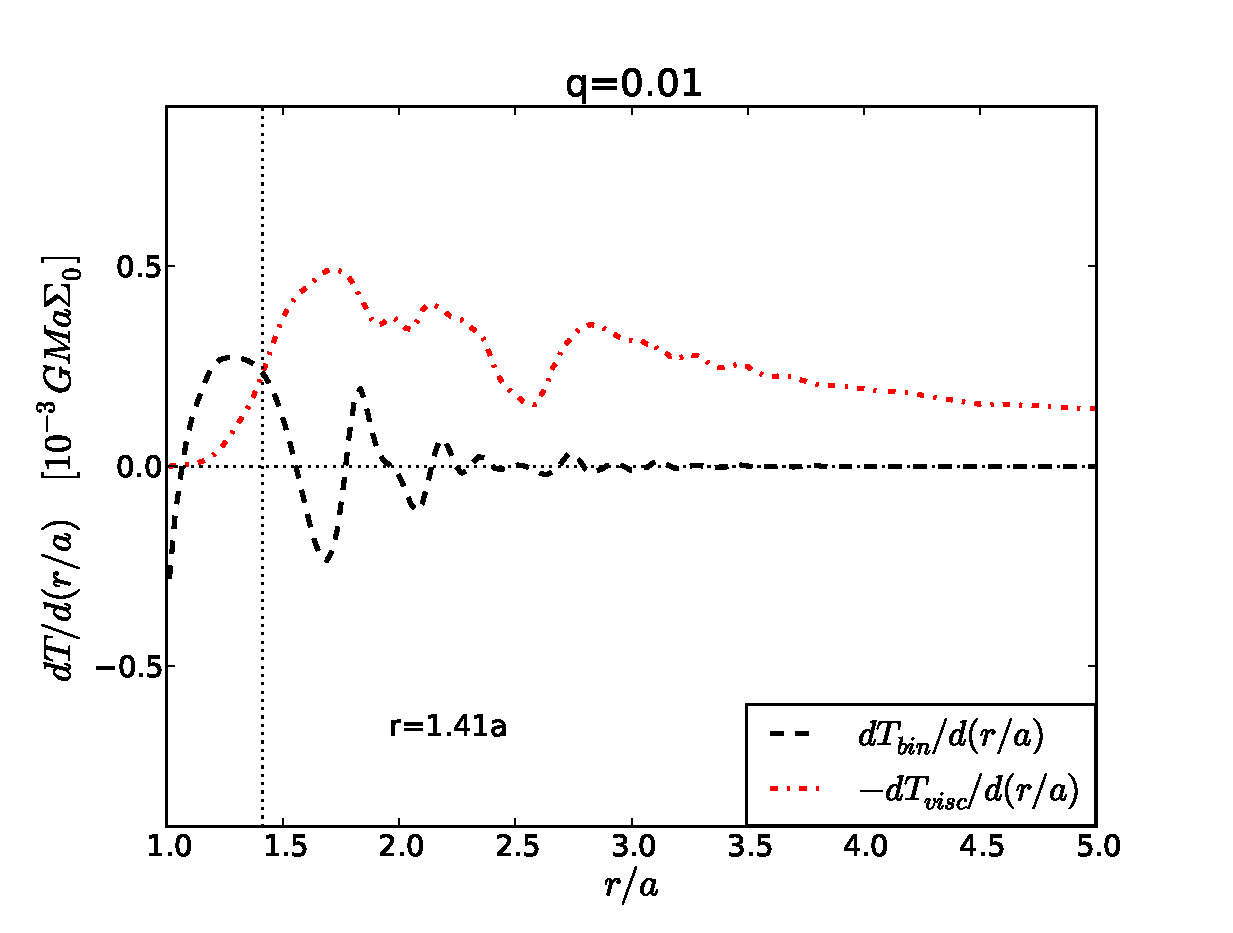
\includegraphics[scale=0.445]{figures/ch1/TRQDENS_LATE_FulVsc_a01_q001_Resr24y78.eps} 
\end{array}$
\caption{Azimuthally- and time-averaged torque density profiles in the
  inner disc for the equal--mass binary (top two panels) and for
  unequal-mass binaries (other panels, with different mass ratios $q$
  as labeled). The top left panel corresponds to the point-symmetric
  transient stage (after $\sim$ 2000 orbits) and the top right panel to
  the asymmetric quasi-steady state (after $\sim$ 4000 orbits).  Only
  the quasi-steady state is shown for the $q<1$ cases. In each panel,
  the dashed [black] curves show the gravitational torques from the
  binary, and the red [dot-dashed] curves show the \textit{negative}
  viscous torques.  The vertical dotted line marks the radius where
  the viscous and gravitational torques balance (equation
  \ref{TrqBalRCE}); these are close to where the azimuthally-averaged
  surface density profiles are found to be truncated (see
  Fig. \ref{AzAvDens}). See Figure \ref{RCE} for a plot of this cavity edge radius vs. $q$. 
  Time averages are taken over 25 orbits at a sample rate of 20 per orbit. }
\label{TrqDq}
\end{center}
\end{figure*}


The top row of Figure \ref{TrqDq} shows the binary and viscous torque
densities for $q=1$ over the inner $5 r/a$ of the disc, during both
the initial transient state (left panel) and the subsequent
quasi-steady-state (right panel).  There is indeed a well-defined
central region, where the binary torques exceed the viscous torques
and can be expected to clear a cavity. The transition (computed via
eq. \ref{TrqBalRCE}) is located at $r_{\rm ce}\simeq1.85$ and
$r=2.02a$ in the transient and quasi-steady-state, respectively, and
is marked in both panels by a vertical dotted line.  These vertical
lines are also shown in Figure \ref{AzAvDens} and indeed lie very
close to radii where the disc surface densities remain truncated.

The small outward drift of the average position of the cavity wall
from the transient to the quasi-steady-state is also visible in Figure
\ref{AzAvDens}. As the disc transitions to the quasi-steady-state, the
binary torque-density wavelength increases in $r/a$, while keeping
approximately the same amplitude.  These effects can be attributed to
the increasingly elongated and lopsided shape of the inner cavity;
when azimuthally averaged, this results in a larger cavity size.


\subsubsection{Accretion Rates}

%%%ACCRETION  RATE vs. t
\begin{figure*}
\begin{center}$
\begin{array}{cc}
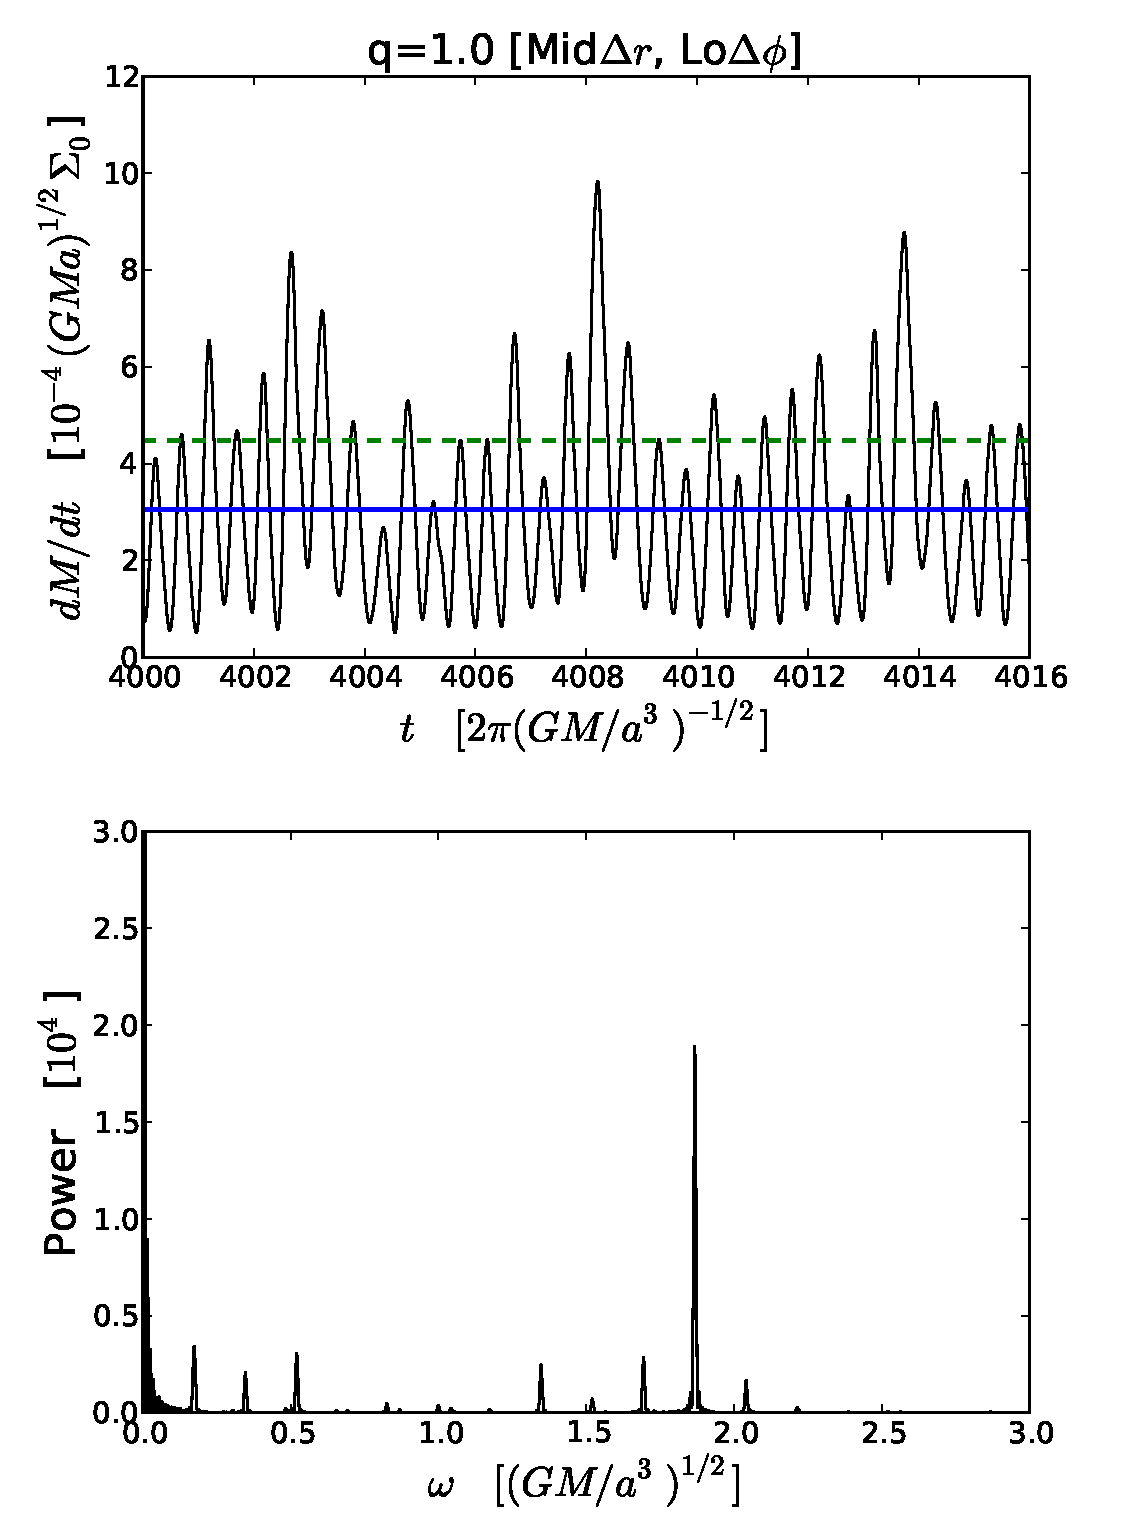
\includegraphics[scale=0.42]{figures/ch1/Mdot_vs_t_q1_FulVsc_alph01_ResMidLo.pdf} &
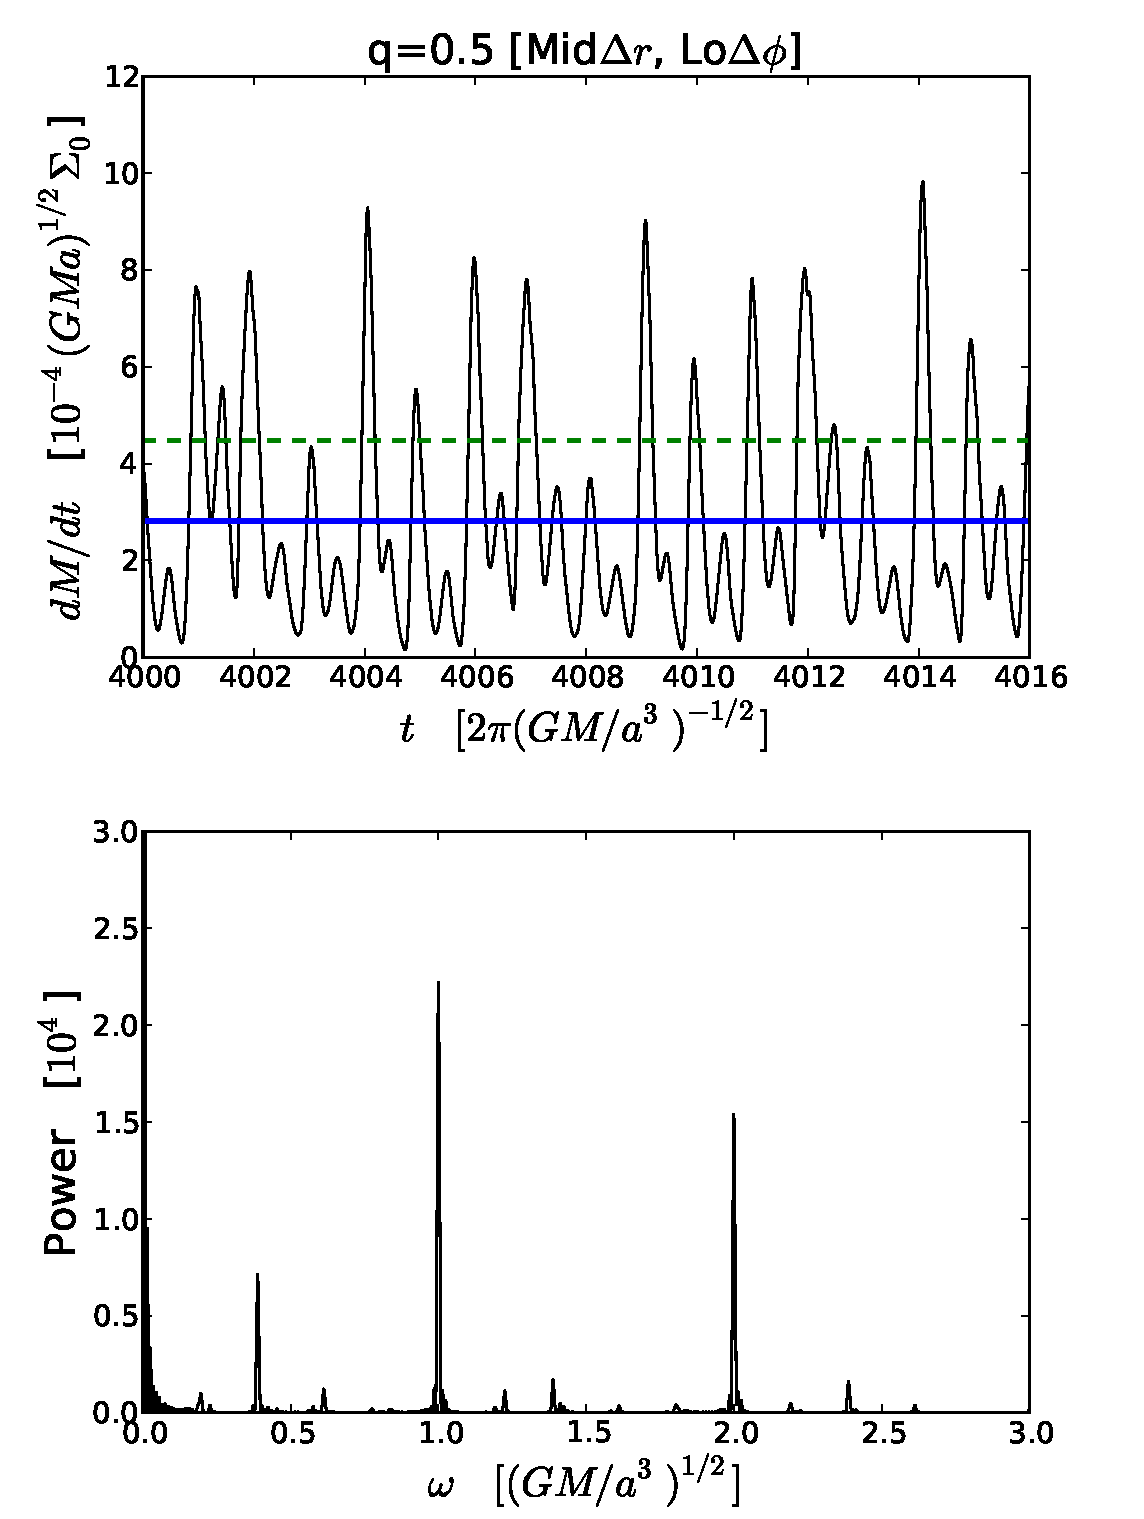
\includegraphics[scale=0.42]{figures/ch1/Mdot_vs_t_q05_FulVsc_alph01_ResMidLo.pdf} \\
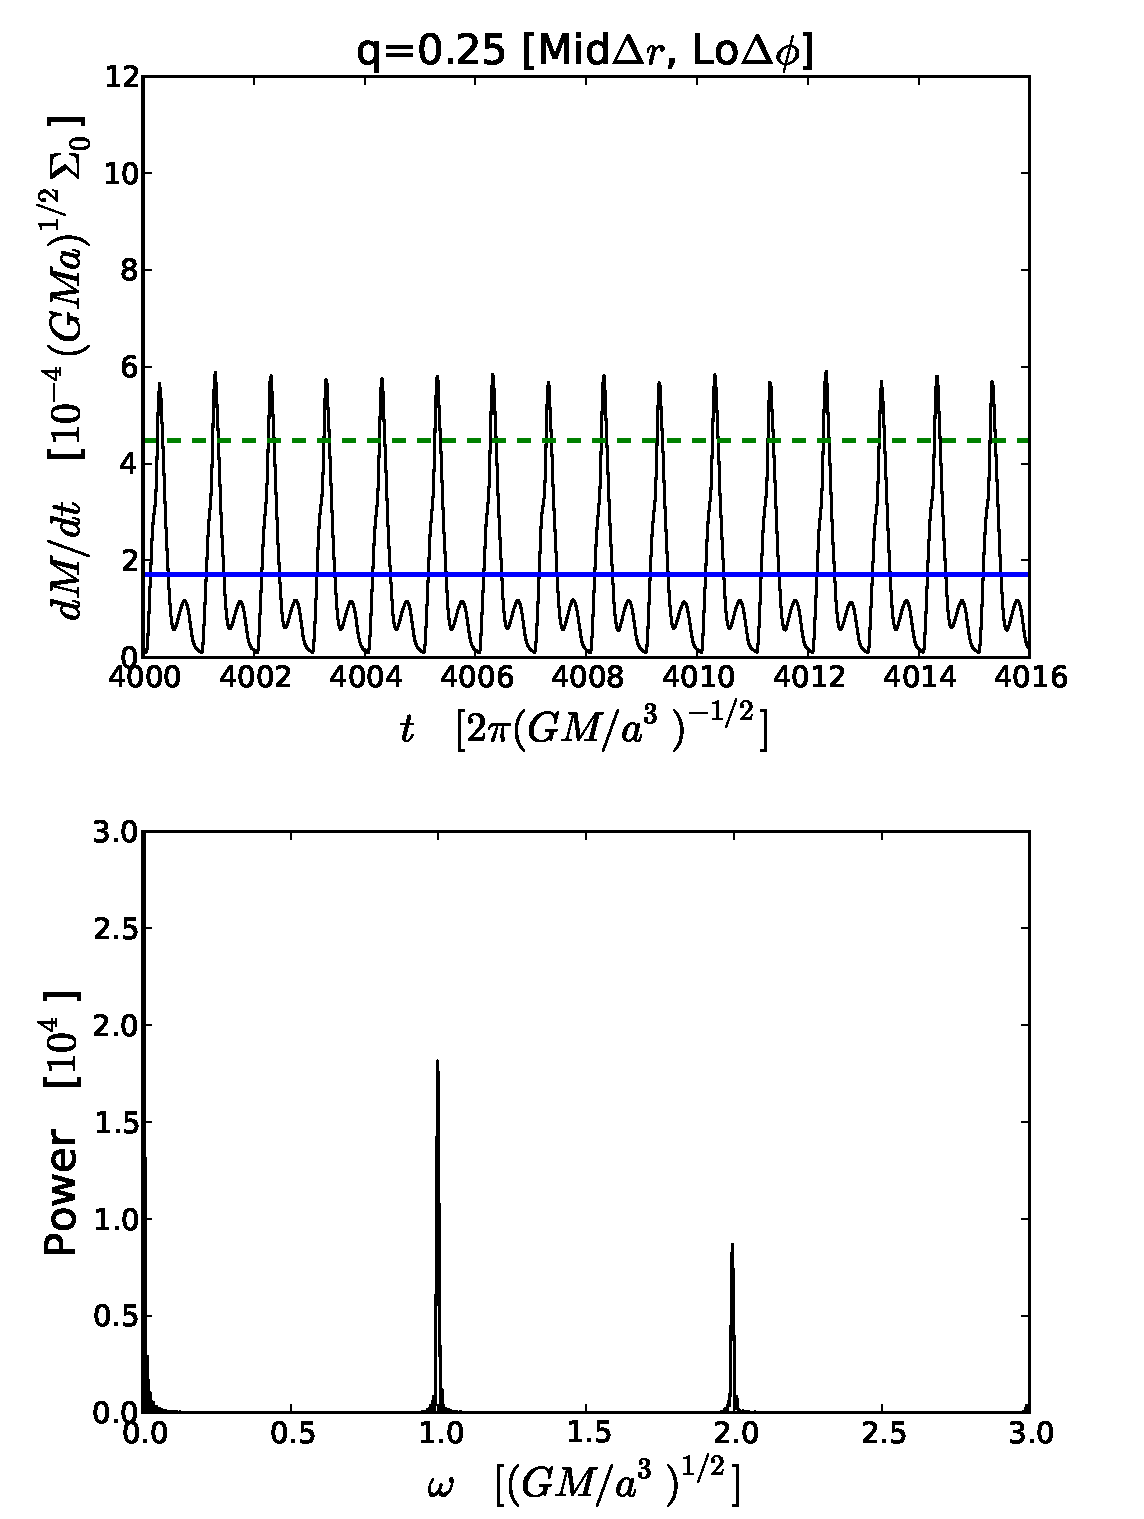
\includegraphics[scale=0.42]{figures/ch1/Mdot_vs_t_q25_FulVsc_alph01_ResMidLo.pdf}  &
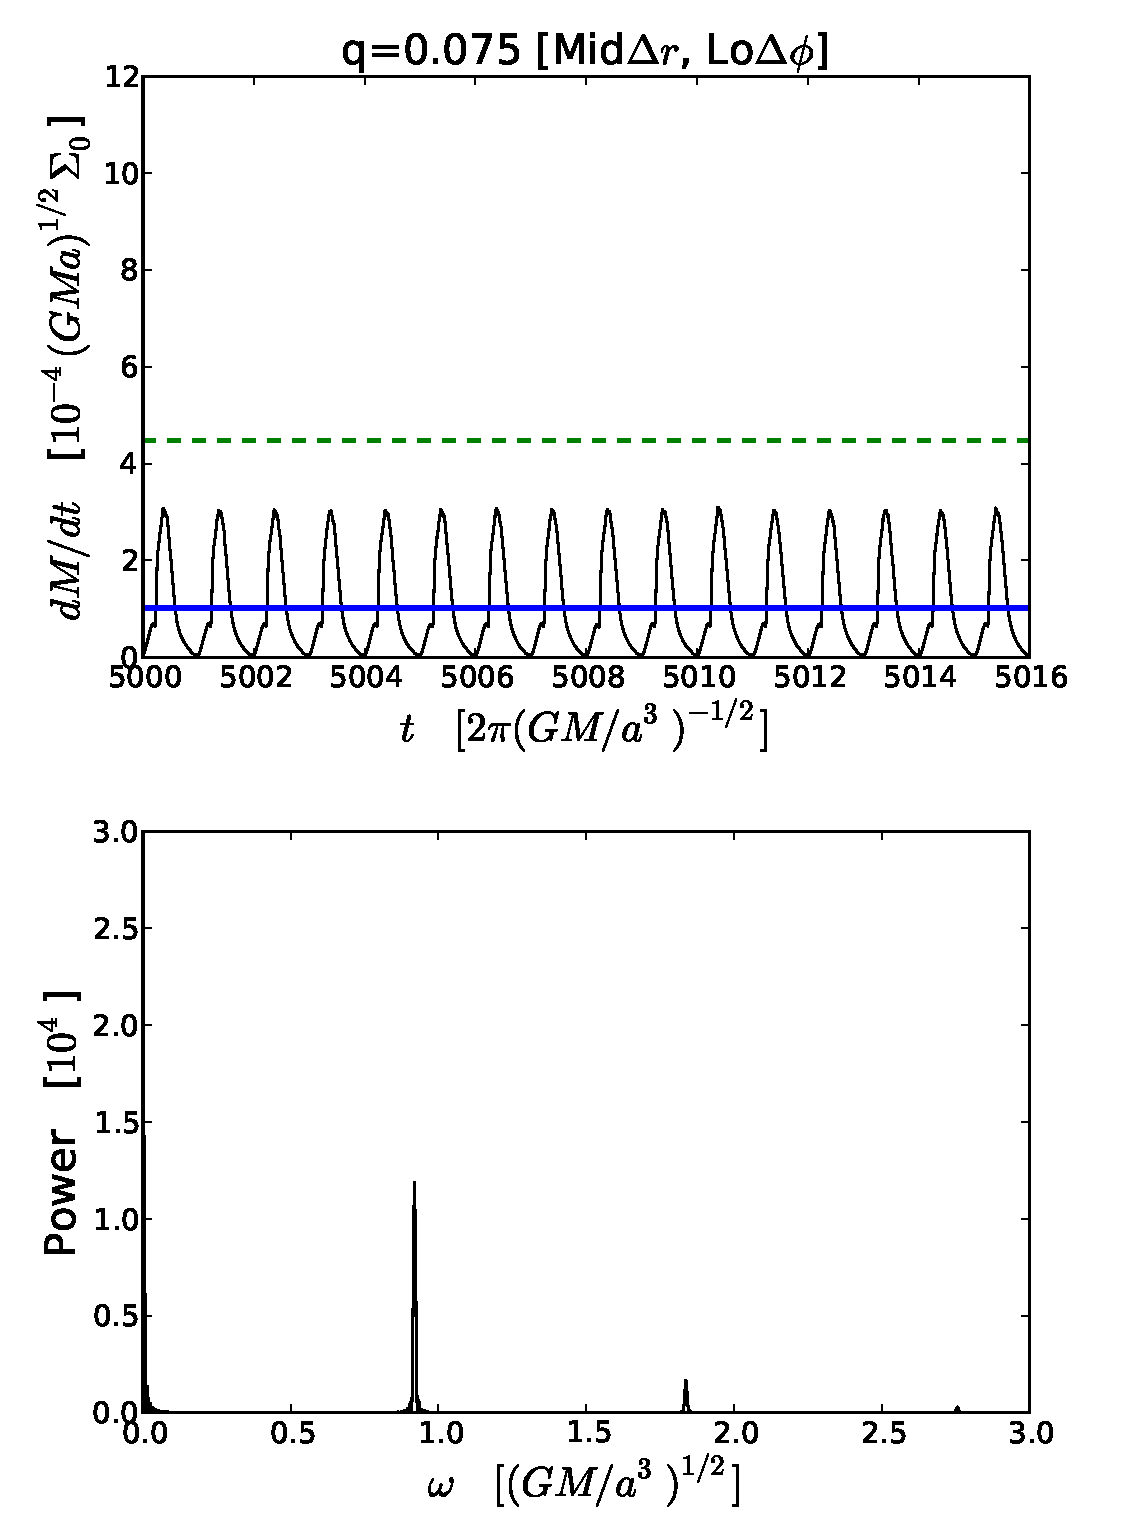
\includegraphics[scale=0.42]{figures/ch1/Mdot_vs_t_q075_FulVsc_alph01_ResMidLo.pdf} 
\end{array}$
\end{center}
\caption{ -- continued on next page}
\end{figure*}


\addtocounter{figure}{-1}

\begin{figure*}
\begin{center}$
\begin{array}{cc}
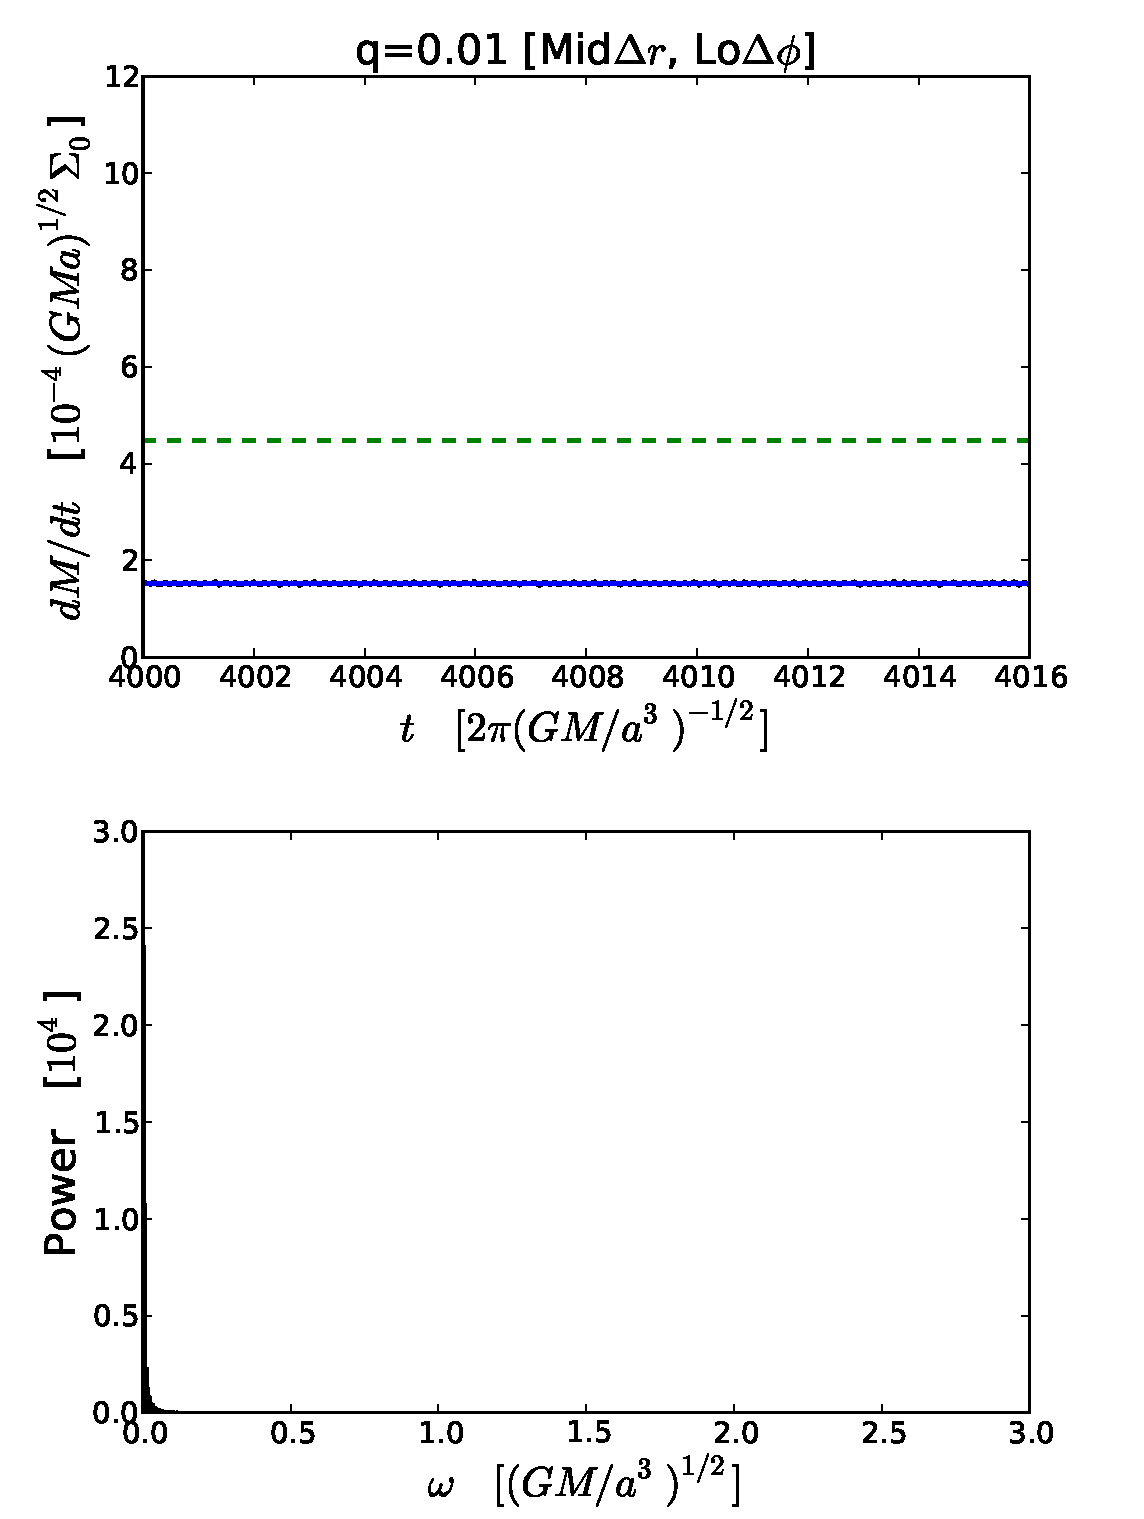
\includegraphics[scale=0.42]{figures/ch1/Mdot_vs_t_q001_FulVsc_alph01_ResMidLo.pdf} &
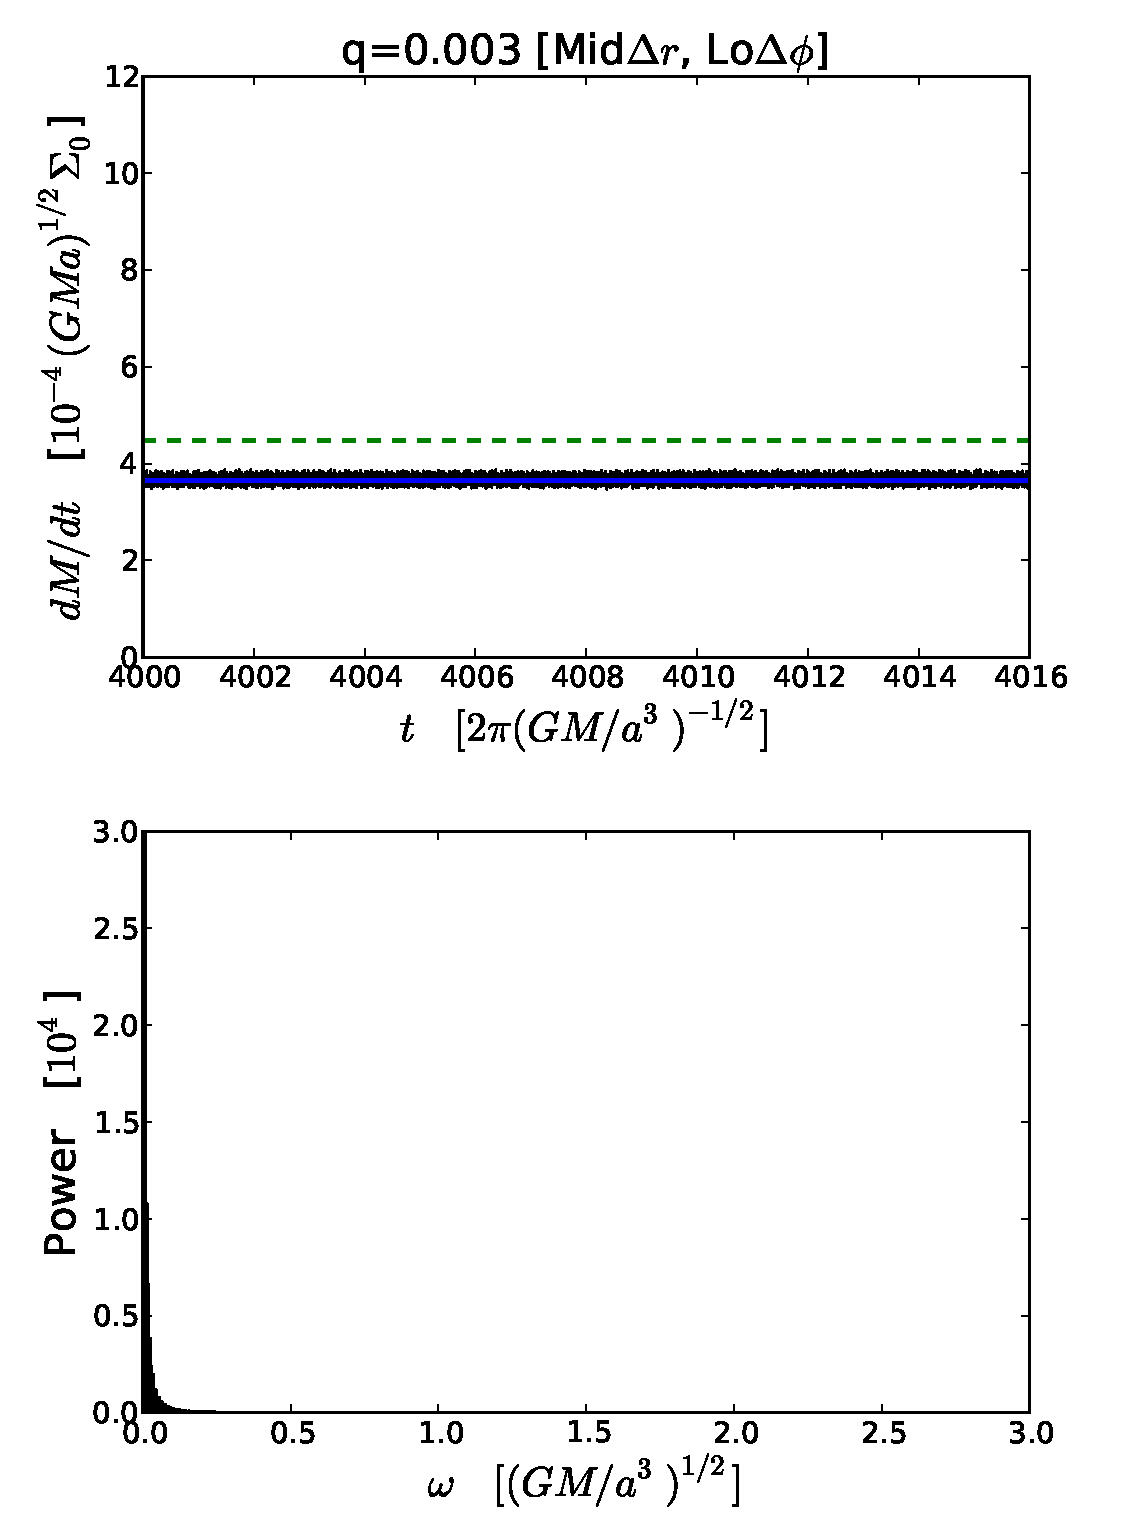
\includegraphics[scale=0.42]{figures/ch1/Mdot_vs_t_q0003_FulVsc_alph01_ResMidLo.pdf} 
\end{array}$
\end{center}
\caption{The time variable accretion rate across the inner boundary of
  the simulation measured at $r=r_{\rm min}=a$ (top of each pair of
  panels) and the corresponding Lomb-Scargle periodogram (bottom of
  each pair) computed over 100 orbits.  Panels are displayed in order of decreasing binary mass
  ratio, starting from $q=1.0$ at top left (on the previous page) to
  $q=0.003$ at the bottom right (on this page). The average accretion
  rate in each panel is denoted by the solid [blue] horizontal line.
  The dashed [green] horizontal line in each plot shows the average
  accretion rate for the point mass ($q=0$) case for reference.  For
  $q>0.05$, the accretion rate is strongly modulated by the binary,
  with either one, two, or three distinct periods present
  simultaneously, depending on the value of $q$ (see text for detailed
  explanations). For $q \lsim 0.05$, the binary still reduces the mean
  accretion rate noticeably, but does not imprint strong periodicity;
  the $q=0.003$ binary is nearly indistinguishable from a single BH.}
\label{Mdott6}
\end{figure*}


The most interesting consequence of the lopsided cavity shape is on
the accretion rate.  In the top left pair of panels in
Figure~\ref{Mdott6}, we show the accretion rate, measured across the
inner boundary of the simulation ($r_{\rm min}=a$) during the
quasi-steady-state, after 4000 binary orbits.  The upper panel shows
the accretion rate as a function of time for $\sim$ 16 binary
orbits; the solid horizontal [blue] line shows the time-averaged
accretion rate during this time, and, for reference, the horizontal
dashed [green] line shows the accretion rate over the same orbits in
the $q=0$ reference simulation. The average accretion
rate onto the binary is approximately $2/3$ of the accretion measured 
for the $q=0$ run at the same resolution. Note that this ratio stays constant 
over the course of the quasi-steady-state.
The lower panel shows the corresponding Lomb-Scargle periodogram, measured over
100 binary orbits at a sampling rate of once per simulation time step
($\sim 500$ per orbit).

As mentioned above, once the quasi-steady-state is reached, the
accretion rate increases from that in the transient state by an order
of magnitude.  As Figure~\ref{Mdott6} shows, it also begins to exhibit
strong (factor of $\sim 3$ above average) variability.  Although this figure samples
the accretion only between 4000 and 4016 orbits, the pattern is
remarkably steady, and repeats itself until the end of the simulation (However, see bullet \ref{vi} in \S \ref{Viscosity Study}). 


The accretion is clearly periodic, and displays two prominent
periods, $(1/2)t_{\rm bin}$ and $\sim5.7t_{\rm bin}$.  The stronger
variability at one half the orbital-time is due to the passage of each
black hole by the near side of the lopsided disc and the corresponding
stripping of gas streams from the cavity wall. These streams are then
driven into the opposite side of the cavity (as seen in the top right
panel in Figure~\ref{2DDensProf}; approximately 135 degrees from the
generation point).  The second, longer timescale corresponds to the
orbital period at the cavity wall.  As mentioned above, when the
non-accreted material from the streams hits the far-side of the
cavity, it creates an over-density which orbits at the disc's
orbital period there which ranges from $\sim 2 \pi (2.0a)^{3/2} (GM)^{-1/2} \sim
2.9\rm{t}_{\rm{bin}}$ out to $\sim2 \pi (3.3a)^{3/2} (GM)^{-1/2} \sim
6.0\rm{t}_{\rm{bin}}$. The larger streams pulled from the lump in turn create 
a new lump and the cycle repeats once every $\sim 5.7 \rm{t}_{\rm{bin}}$.
Similar over-dense lumps have also been found
and described in the 3D MHD simulations of \cite{ShiKrolik:2012}; more
recently, \cite{RoedigDotti:2011, Roedig:2012} have also mentioned the
contributions of such lumps to fluctuations in the accretion rate.



\subsection{Unequal-Mass Binaries}
\label{Unequal-Mass Binaries}

We next turn to the main new results of this paper, and examine the
disc behaviour as a function of the mass ratio.  We start with a
qualitative description of how the accretion pattern changes as we
decrease $q$.

\subsubsection{Three-Timescale Regime: $0.25 < q < 1$.}
\label{Three Timescale Regime}


%%% Mdot RATIOS TABLE
\begin{table*}
\begin{center}
 \caption{The mean accretion rate $\dot{M}_{\rm bin}$, averaged over
    1000 orbits in the quasi-steady-state, for binaries with different
    mass ratios.  The rates are shown in units of the corresponding
    rate $\dot{M}_{q0}$ found in a single-BH ($q=0$) simulation.  
    This ratio is computed as an average from $3500$ to $4500$ orbits unless the quasi-steady 
    state isn't reached until after (or for large $\alpha$ much before) $3500$ orbits; in this case the value 
    in the table is denoted by $^*$.The first four rows show results for 
    different combinations of radial and azimuthal resolutions. 
    The first row is our fiducial resolution. The last three rows are for runs at the 
    fiducial resolution but different magnitudes of the viscosity parameter $\alpha$.}
\label{Mdot_ratios}
\begin{tabular}{l  |  c c c c c c c c c c}
                                     $q$                                   & 1.0   & 0.75 &  0.5 &  0.25   & 0.1   & 0.075  & 0.05 & 0.025 & 0.01 & 0.003 \\ \hline
    $\dot{M}_{\rm{bin}} / \dot{M}_{q0}  \left[\rm{Mid}\Delta r, \rm{Lo}\Delta \phi \right]$   & 0.671 &  0.700 & 0.655 & 0.382   & 0.355$^*$ & 0.228$^*$  & 0.025 & 0.100  & 0.341 &  0.814  \\                                   
  $\dot{M}_{\rm{bin}} / \dot{M}_{q0}  \left[\rm{Lo}\Delta r, \rm{Lo}\Delta \phi \right]$     & 0.544 & 0.518 & 0.499 & 0.406  & 0.021  & 0.027  & 0.055 & 0.147 & 0.381 &  \\  
  $\dot{M}_{\rm{bin}} / \dot{M}_{q0}  \left[\rm{Mid}\Delta r, \rm{Mid}\Delta \phi \right]$ & 0.821 &  &  &  &  0.426  &   & 0.028 & & &  \\
  $\dot{M}_{\rm{bin}} / \dot{M}_{q0}  \left[\rm{Hi}\Delta r, \rm{Hi}\Delta \phi \right]$      & 0.930 &  &  &  &  0.724 &   & 0.172$^*$  &   &  &  \\
  $(\alpha = 0.02$)                                            							        & 0.899 &    &    &     &   &    &  &   &  &    \\
  $(\alpha = 0.04$)                                           						    	        & 0.921 &    &    &     &   &    &  &   &  &    \\
  $(\alpha = 0.1$)                                    								        & 1.015$^*$ &    &    &     &   &    &  &   &  &    
  \end{tabular}
 \end{center}
\end{table*}
%%%%%%%%%%%%%%%%%

%%%%%%%%%%%%%%%%%%%%%%%%%%%%%%%%%%
%%%Mdot_bin / Mdot_q0
\begin{figure}
\begin{center}$
\begin{array}{cc}
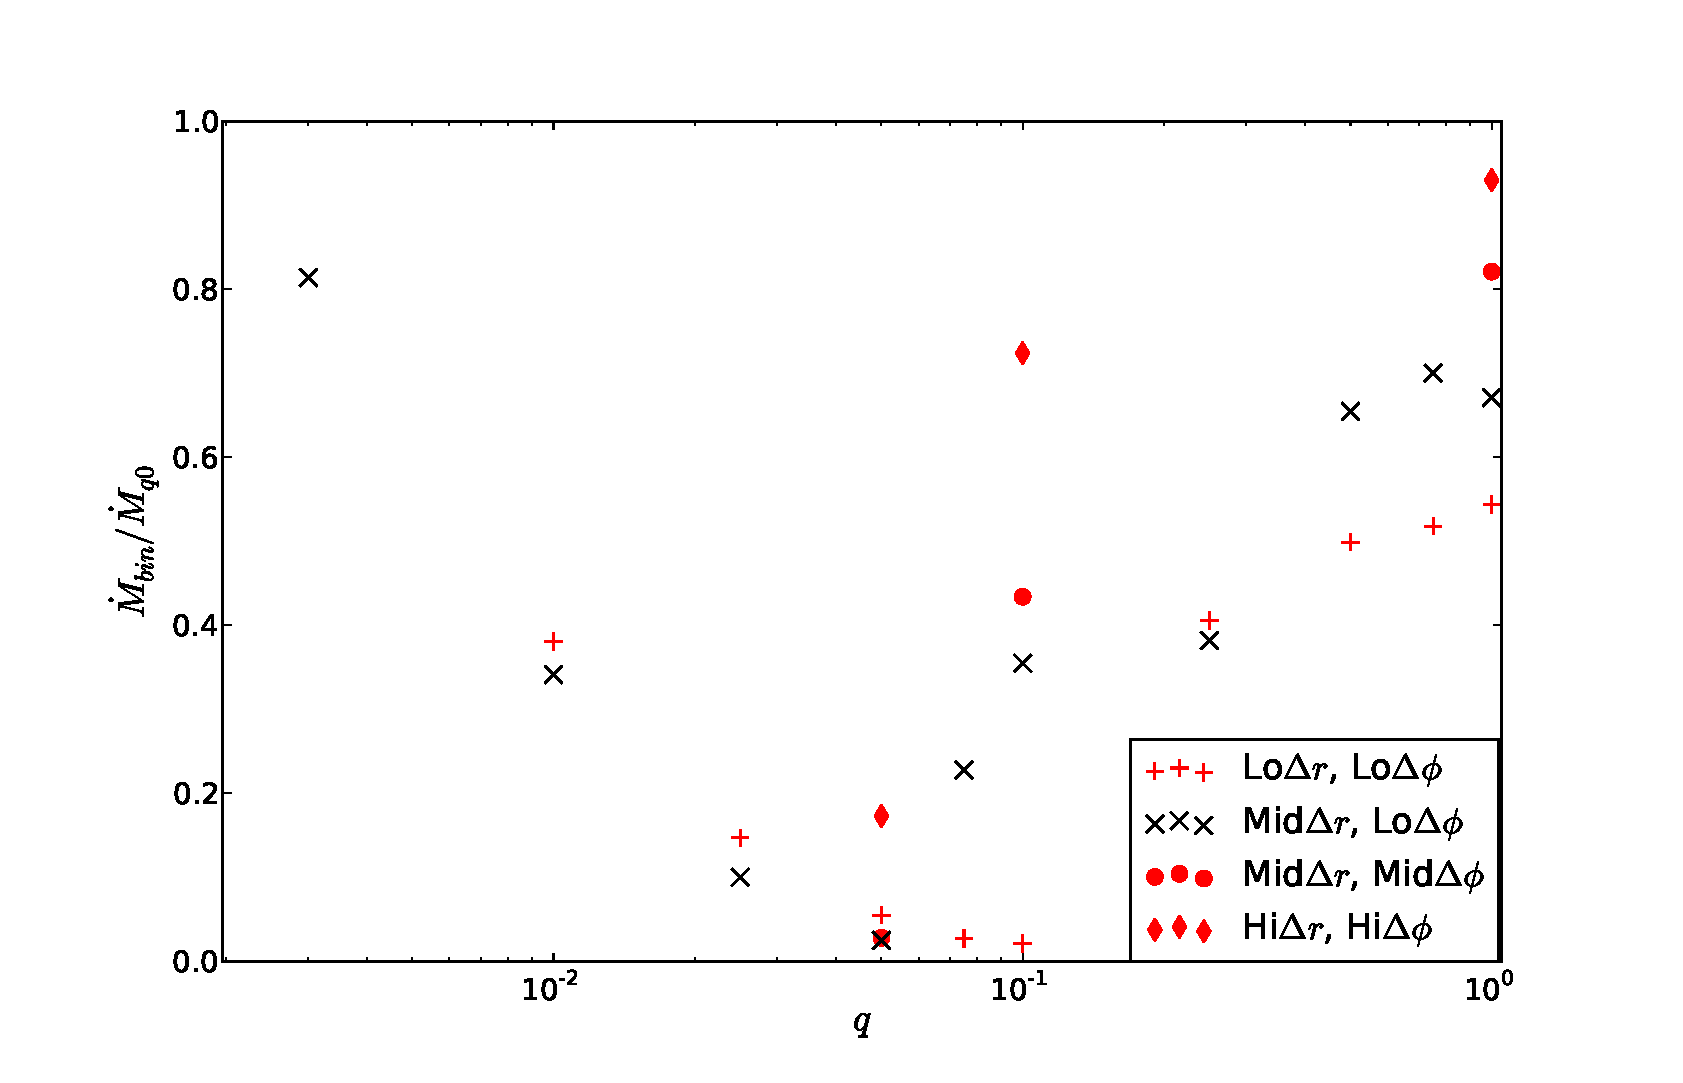
\includegraphics[scale=0.3]{figures/ch1/Mbin_o_Mq0.eps} 
\end{array}$
\end{center}
\caption{The average mass accretion rate as a function of $q$, and for
  simulations with different spatial resolution.  This is the same
  information as in Table \ref{Mdot_ratios}, except here shown
  graphically and with only the simulations at the fiducial magnitude of viscosity.}
\label{Mdot_ratios_plot}
\end{figure}
%%%%%%%%%%%%%%%%%%%%%%%%%%%%%%%%%%

The behaviour of systems with mass ratio in the range $0.25 \lsim q <
1$ are illustrated in Figures \ref{2DDensProf}, \ref{AzAvDens} and
\ref{Mdott6}.  These show snapshots of the 2D surface density in the
quasi-steady-state, the evolution of the azimuthally averaged density
profile, and the time-dependent accretion rates, respectively.
Additionally, in Table~\ref{Mdot_ratios}, and in the corresponding
Figure~\ref{Mdot_ratios_plot}, we show the time-averaged accretion
rate as a function~of~$q$.  In each case, the accretion rate is
averaged over 1000 binary orbits in the quasi-steady state (unless noted, from 3500-4500 binary orbits), and is quoted in
units of the corresponding rate for a single-BH $(q=0)$ disc. This ratio changes very little over the course of the quasi-steady-state regime.

These figures and table illustrate several trends as $q$ is lowered
from $q=1\rightarrow 0.75 \rightarrow 0.5 \rightarrow 0.25$:

\begin{enumerate}

\item The cavity becomes more compact, and less lopsided, as one
  naively expects when the binary torques are reduced. These effects
  are clearly visible in the middle row of Figure~\ref{2DDensProf},
  and also in the corresponding azimuthally averaged density profiles
  in Figure~\ref{AzAvDens}: the profiles look remarkably similar for
  $q=0.5$ and $0.25$, except the cavity for $q=0.25$ is smaller, and its
  wall is visibly sharper (as a result of azimuthally averaging over a
  less lopsided 2D distribution).

\item The secondary (primary) moves closer to (farther from) the cavity
  wall as $q$ is reduced. 
  Thus occurs for two reasons. First, the position of the secondary (primary) moves
  away from (towards) the binary's center of mass,
  %
  \begin{align}
  r_s(q)= a(1+q)^{-1} \qquad \qquad  r_p(q) = a(1+1/q)^{-1}.
  \end{align}
  %
  Second, as mentioned in (i), the size of the central cavity decreases. 
  (Fig.~\ref{AzAvDens}) shows the locations of
  the cavity edge $r_{\rm ce}$ expected from balancing the azimuthally
  averaged gravitational and viscous torques (Fig. \ref{TrqDq}), which
  agree well with the observed cavity sizes. In Figure
  \ref{RCE}, we explicitly show $r_{\rm ce}$ as a function of $q$.  The
  points in the figure have been obtained by balancing the azimuthally
  averaged viscous and gravitational torques measured in the simulation
  (equation \ref{TrqBalRCE}).  The black line is an empirical fit to the
  data points at fiducial resolution, given by
  \begin{align}
  r_{\rm ce}(q) &\simeq A + B \ \rm{ln} \left( q^{1/2} + 1\right) + C \ \mbox{ln} \left( q + 1\right)    \nonumber  \\ 
  A &=1.191 \qquad
  B =2.541 \qquad
  C =-1.350
  \label{EmpFitrce}
  \end{align}
  
%%%%%%%%%%%%%%%%%%%%%%%%%%%%%%%%%%%%%%%%
%%%Cavity Edge 
\begin{figure}
\begin{center}$
\begin{array}{c}
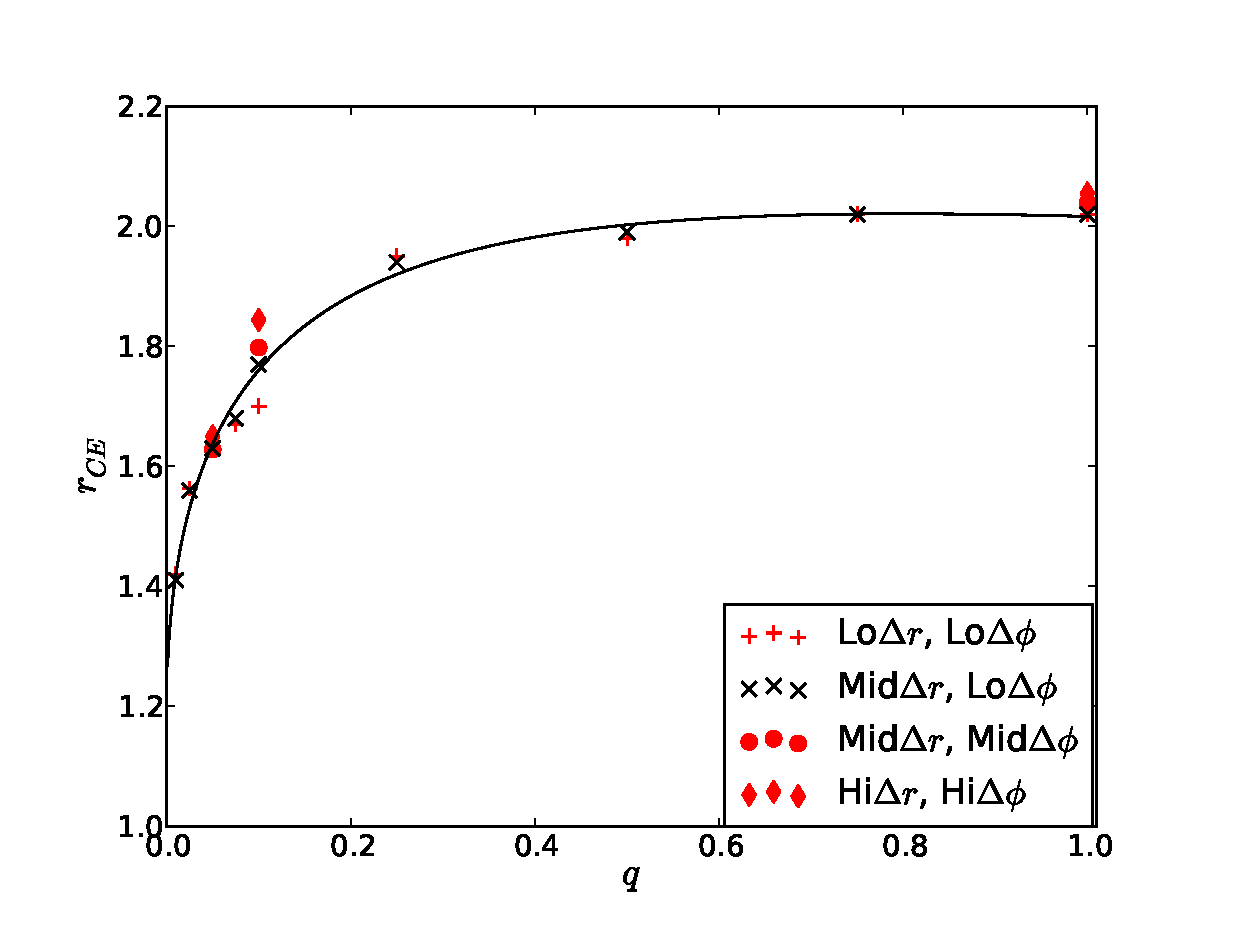
\includegraphics[scale=0.4]{figures/ch1/RCE_2LogFit.eps}  
\end{array}$
\end{center}
\caption{The position of the cavity wall as a
  function of $q$, in runs with different radial and azimuthal 
  resolutions, as labeled.  The
  points mark the radii $r_{\rm ce}$ at which the azimuthally averaged
  viscous and gravitational torques balance (equation
  \ref{TrqBalRCE}). The black line is an empirical fit to the fiducial resolution data
  points (equation \ref{EmpFitrce}).  }
\label{RCE}
\end{figure}
%%%%%%%%%%%%%%%%%%%%%%%%%%%%%%%%%%%%%%%%

\item The dense lump, created by the shocks due to the
  ``regurgitated'' stream-material thrown back out by the binary, is
  still present for $q=0.5$ (see the corresponding panel in
  Fig.~\ref{2DDensProf}, around 9 o'clock at $r\sim 2a$), but
  is much less discernible for $q=0.25$.  Again, this trend is
  unsurprising - as the torques diminish, one expects weaker shocks
  and smaller over-densities in any resulting lump.

\item The accretion streams in the $q=0.25$ panel of
  Figure~\ref{2DDensProf}, and the corresponding ripples in the azimuthally averaged density profiles of Figure~\ref{AzAvDens}, become noticeably weaker.  However, the
  average accretion rate, shown in Figures \ref{Mdott6}
  and~\ref{Mdot_ratios_plot} and in Table~\ref{Mdot_ratios}, stays at
  approximately $\simeq 0.7 \dot{M}_{q0}$ over the range $0.5 \lsim q \leq 1$. For
  $q \lsim 0.5$, the average accretion rate drops more rapidly,
  falling by nearly a factor of two to $\simeq 0.36 \dot{M}_{q0}$ by
  $q=0.1$. 
  
\item As the average accretion rate decreases, so does the maximum
  accretion rate (i.e., the amplitude of the spikes in
  Fig.~\ref{Mdott6}) keeping an approximately constant enhancement factor of $\sim3$
  as the mass ratio is decreased to
  $q\sim 0.1$.  
  

\item The percentage of a stream which leaves the domain at $r_{\rm{min}} =a$ as opposed to being flung back out also decreases by a factor of $\sim2$ as $q$ decreases from 1.0 to 0.1. We measure this 
  percentage from the simulations by computing the ratio $\dot{M}(r_{95})/\dot{M}(r_{\rm min})$ averaged over 25 orbits in the quasi-steady-state. Here $r_{95} = 0.95 r_{\rm{ce}}$ (with $r_{ce}$ given by equation 
  (\ref{EmpFitrce})) is chosen to be just inside the cavity wall where the accretion rate is dominated by the streams. The percentage drops by approximately a factor of two, from $\sim 3.3 \%$ at $q=1$ to 
  $\sim1.8 \%$ at $q=0.1$ suggesting that the drop in average accretion rate in the three-timescale regime is due largely to the amount of stream material which can penetrate beyond the binary torque barrier at small $r$.


\item Perhaps the most interesting result is shown by the Lomb-Scargle
  periodograms in Figure \ref{Mdott6}. As $q$ decreases, power is
  traded from both the $(1/2)t_{\rm bin}$ and the $5.7t_{\rm
    bin}$ variability timescales into the $t_{\rm bin}$ timescale.
  This is because of the increased proximity between the secondary and
  the cavity wall, and a corresponding larger distance between the
  primary and the cavity wall noted above.  As a result, as $q$ is
  decreased, the secondary begins to dominate the variability, pulling 
  accretion streams off of the cavity wall once per binary orbit.

\end{enumerate}


Focusing on the last finding: in the $0.25 \lsim q < 1$ case, we find
that the time-dependent accretion rate displays {\em three distinct
  and sharply defined periods}, with well-defined ratios at $0.5, 1$,
and $5.7t_{\rm bin}$.  While the last of these reflects the orbit of the
dense lump at the elongated cavity wall and could depend on details of the disc
properties, the first two periods are fixed by the binary alone and
are independent of the disc.  {\em The 1:2 period ratio is therefore a
robust prediction; if observed, it could serve as a smoking gun
signature of a binary.}



\subsubsection{Single-Orbital-Timescale Regime: $0.05 \lsim q \lsim 0.25$.}
\label{Orbital Timescale Regime}

As $q$ is further decreased, the overall distortions to the disc
become less pronounced, and approach a nearly axisymmetric, tightly
wound spiral pattern (see the $q=0.075$ panel in
Figure~\ref{2DDensProf}).  The distance between the cavity wall and
the secondary further shortens, and the accretion variability becomes
dominated entirely by the streams created by the secondary's passage
once per orbit.  As Figure \ref{Mdott6} shows, for $q=0.075$ the accretion rate displays a nearly sinusoidal
variation, with the corresponding Lomb-Scargle periodogram showing a
single spike just offset from the orbital timescale of the binary.
For $q=0.075$,
the fluctuations are still large (factor of $\sim 3$), but by
$q=0.05$, the fluctuations disappear.  Interestingly,
we find that the average accretion rate is most strongly suppressed
among all of our runs in a narrow mass ratio range $q \sim0.05 \pm 0.0025$; by up to a factor of $\sim 40$ compared
to the single-BH case. However, for out highest resolution run at $q=0.05$, we no longer observer this extreme dip in average accretion rates (see \S \ref{Resolution Study}).

As mentioned above, the disappearance of the $(1/2) t_{\rm bin}$
variability timescale is easy to understand qualitatively: once the
primary BH remains very close to the center-of-mass, its compact
orbital motion no longer impacts the disc far away.  The disappearance
of the $5.7 t_{\rm{bin}}$ variability timescale is also clearly
attributable to the lack of any dense lump near the cavity wall for
$q\lsim 0.25$.  However, the reason this lump disappears is less
obvious, and warrants some discussion.


\begin{enumerate}
\item As $q$ decreases, the cavity becomes less lopsided, and the
  accretion rate spikes become weaker.  This suggests that when these
  weaker accretion streams are flung back to the cavity wall, they
  create less over-dense lumps.  For $q \leq 0.25$, the lump may not
  survive shear stresses and pressure forces, and may dissolve in less
  than an orbital time.
\item As can be eyeballed from Figure \ref{2DDensProf}, the stream
  impact zone (dense region outside the cavity) extends over an
  azimuth of $\Delta\phi \sim 100-120^{\circ}$. The orbital period at
  the cavity edge is $\leq 6 t_{\rm bin}$ (the orbital period at the furthest edge of the cavity), implying that multiple
  streams can hit parts of the same lump if streams are
  generated more than once per binary orbit.
\end{enumerate}


To test whether the strength or the frequency of the streams is more
important for lump generation, we repeat our simulation for an
equal-mass binary, but we placed one of the BHs artificially at what
would be the real binary's center of mass. The second hole still
orbits at $r=a/2$ as usual.  In this setup, the cavity wall is
perturbed by streams with a similar strength as in the real $q=1$
simulation (however much less of the streams reach the inner edge 
of the simulation domain in this one-armed perturber case), but now only once, rather than twice per orbit. We found
that, while this ``one-armed'' binary does generate significant stream impacts at the cavity edge, it does {\em not} create an orbiting
over-density at the cavity edge, nor does it excite a significant
elongation of the cavity.  We therefore conclude that multiple,
overlapping streams are required to generate a strong lump that
survives for an orbital time. However, as the $q=0.25$ accretion rate and periodogram show in Figure \ref{Mdott6}, simply generating two streams is not a sufficient condition for generating a cavity wall lump. Both streams must also be sufficiently large.
This explains the disappearance of the cavity wall frequency for $q\lsim0.25$; as the mass ratio decreases, the primary generates less significant streams and the overlap of two large streams crashing into the cavity wall can no longer occur to generate an over-dense lump there.
This result is also consistent with the cavity becoming less lopsided as $q$ decreases.


\subsubsection{Steady-Accretion Regime: $q \lsim 0.05$.}
\label{Non-Variable Regime }

As we continue to decrease $q$ from $0.075$ through $0.05$ to $0.01$, we find yet another
distinct regime.  The overall morphology of the snapshot of a $q=0.01$ and $q=0.05$ (not shown)
disc in Figure~\ref{2DDensProf} looks similar to the $q=0.075$ case,
except the nearly-concentric perturbations are even weaker, and the
cavity still smaller.  However, the similarity is quite deceptive,
with the movie versions of these figures showing a striking
difference.\footnote{Movie versions of the snapshots in
  Figure~\ref{2DDensProf} are available at http://www.astro.columbia.edu/$\sim$dorazio/moviespage}
In the $q=0.075$ case, accretion streams form and disappear
periodically, but in the $q=0.05$ case, the disc pattern becomes
constant and unchanging (in the frame co-rotating with the binary).
There is still a visible accretion stream, hitting the inner boundary
of the simulation just ahead of the secondary's orbit, but the stream
steadily co-rotates with the binary.

As Figure \ref{Mdott6} shows (see also Fig.~\ref{Mdot_ratios_plot} and
Table~\ref{Mdot_ratios}), the average accretion rate has reached its
minimum at $q=0.05$. For $q \leq 0.05$, the accretion rate
becomes steady, with no fluctuations, and its value {\em increases}
back towards the $q=0$ rate (dashed horizontal [green] line in Figure
\ref{Mdott6}).  For such a light secondary, the system
begins to resemble a disc with a single BH.  Although a cavity is
still clearly present (moving from $r\simeq1.6a$ at $q=0.05$ to
$r\simeq1.4a$ at $q=0.01$), it is being refilled, as for a single
BH. Indeed, after 4000 orbits, the $q=0.01$ azimuthally averaged density
profile is approaching the $q=0$ profile (see
Fig.~\ref{AzAvDens}). \\


Although the secondary still excites small but visible ripples in the
disc (Fig.~\ref{2DDensProf}), by $q\leq0.05$ it can no longer exert a
large enough torque to pull in large streams and drive them back out
to produce a lopsidedness in the circumbinary disc.  The ripples are 
in the linear regime, and they resemble the tightly-wound
spiral density waves launched in protoplanetary discs
(e.g. \citealt{GT80,DRS:2011:Linear,DM2012}), except here our
background discs have a pre-imposed central cavity.  In the 
linear regime, the waves are excited by resonant interactions with the
disc, and non-linear coupling to an $m=1$ mode is no longer
possible. Note the disappearance of any ripples in the azimuthally
averaged surface density for $q = 0.01$ (Fig.~\ref{AzAvDens}).



\section{Summary and Discussion}
\label{Summary and Discussion}
In summary, we find that the behavior of the accretion rate across the
circumbinary cavity as a function of $q$ can be categorized into four
distinct regimes:

\begin{enumerate}
\item {\em Two-timescale regime; $q=1$.}  Confirming previous
  results, an equal-mass binary maintains a central low-density cavity
  of size $r\sim 2a$ and the time-averaged accretion rate is $\sim2/3$ 
  of that for a point-mass case. There are up to factor of $\sim3$
  fluctuations around the average on two prominent time-scales,
  $(1/2)t_{\rm bin}$ and $\sim 5.7t_{\rm bin}$.
\item {\em Three-timescale regime; $ 0.25 < q < 1$.}  The
  time-averaged accretion rate drops by a factor of $\sim 1.8$ by
  $q=0.25$; however, the maximum fluctuations 
  continue to occur with amplitude $\sim3$ times the average rate . 
  There are three time-scales present, $(1/2)t_{\rm bin}$, $t_{\rm
    bin}$, and $\sim 5.7t_{\rm bin}$.
\item {\em Single-orbital-timescale regime; $0.05 \lsim q < 0.25$.} In
  this regime, the average accretion rate and its fluctuations continue to
  drop with decreasing $q$. Variability is dominated by the secondary, 
  and is nearly sinusoidal on the binary period $t_{\rm bin}$ though accompanied by small accretion spikes due to the primary with maxima below the average rate.
\item {\em Steady-Accretion regime; $q \lsim 0.05$.} The accretion 
  becomes steady while reaching its lowest rate at $q\sim0.05$. By $q=0.003$, the accretion rate rises 
  again to $\sim0.8$ of the $q=0$ case. The system overall resembles a 
  cavity-filling single-BH disc, with small perturbations due to 
  the secondary in the linear regime.
\end{enumerate}




\subsection{Comparison with MM08}
\label{Viscosity Dependence  and Comparison with MM08}
Our main qualitative conclusions for the equal-mass binary case,
including the morphology of the disc, and the accretion rate, are in
good agreement with MM08.  Nevertheless we do find a small 
discrepancy in the time averaged accretion rates.


Comparing MM08's Figures 7 and 8 with the top left panel of
our Figure \ref{MM08_compare}, which is run at the same 
resolution as the highest resolution used in the MM08 study,
%Footnote
\footnote{This refers to the highest resolution used by MM08 at the inner region of the disc. MM08 use a lower resolution far away from the binary where this study uses a uniform resolution throughout.}
%
we see that the magnitudes of the
time-averaged accretion rates, as well as the periodogram frequencies, agree. However, the detailed variability is not identical.

The primary difference is that there is more power at low frequencies in the MM08 periodograms. In-between the largest accretion spikes, the MM08 accretion rate drops closer to zero and becomes less uniform where as our accretion rate is a steady modulation of spikes occurring at the twice the binary orbital period. The accretion rate and periodogram observed in MM08 could be realized if viscous stresses are less efficient at breaking up the over-dense lump responsible for creating the $(5-6) t_{\rm bin}$ modulation. Then the lump will be more centralized and there will be a greater disparity between streams which are generated from the lump and streams which are not. Thus we conjecture that this small difference may be due to different treatments of viscosity and grid setup, or differences between FLASH2 (used by MM08) and FLASH3 (used here). 


%%%Mdot vs. t Low Res MM08 replica
\begin{figure}
\begin{center}
 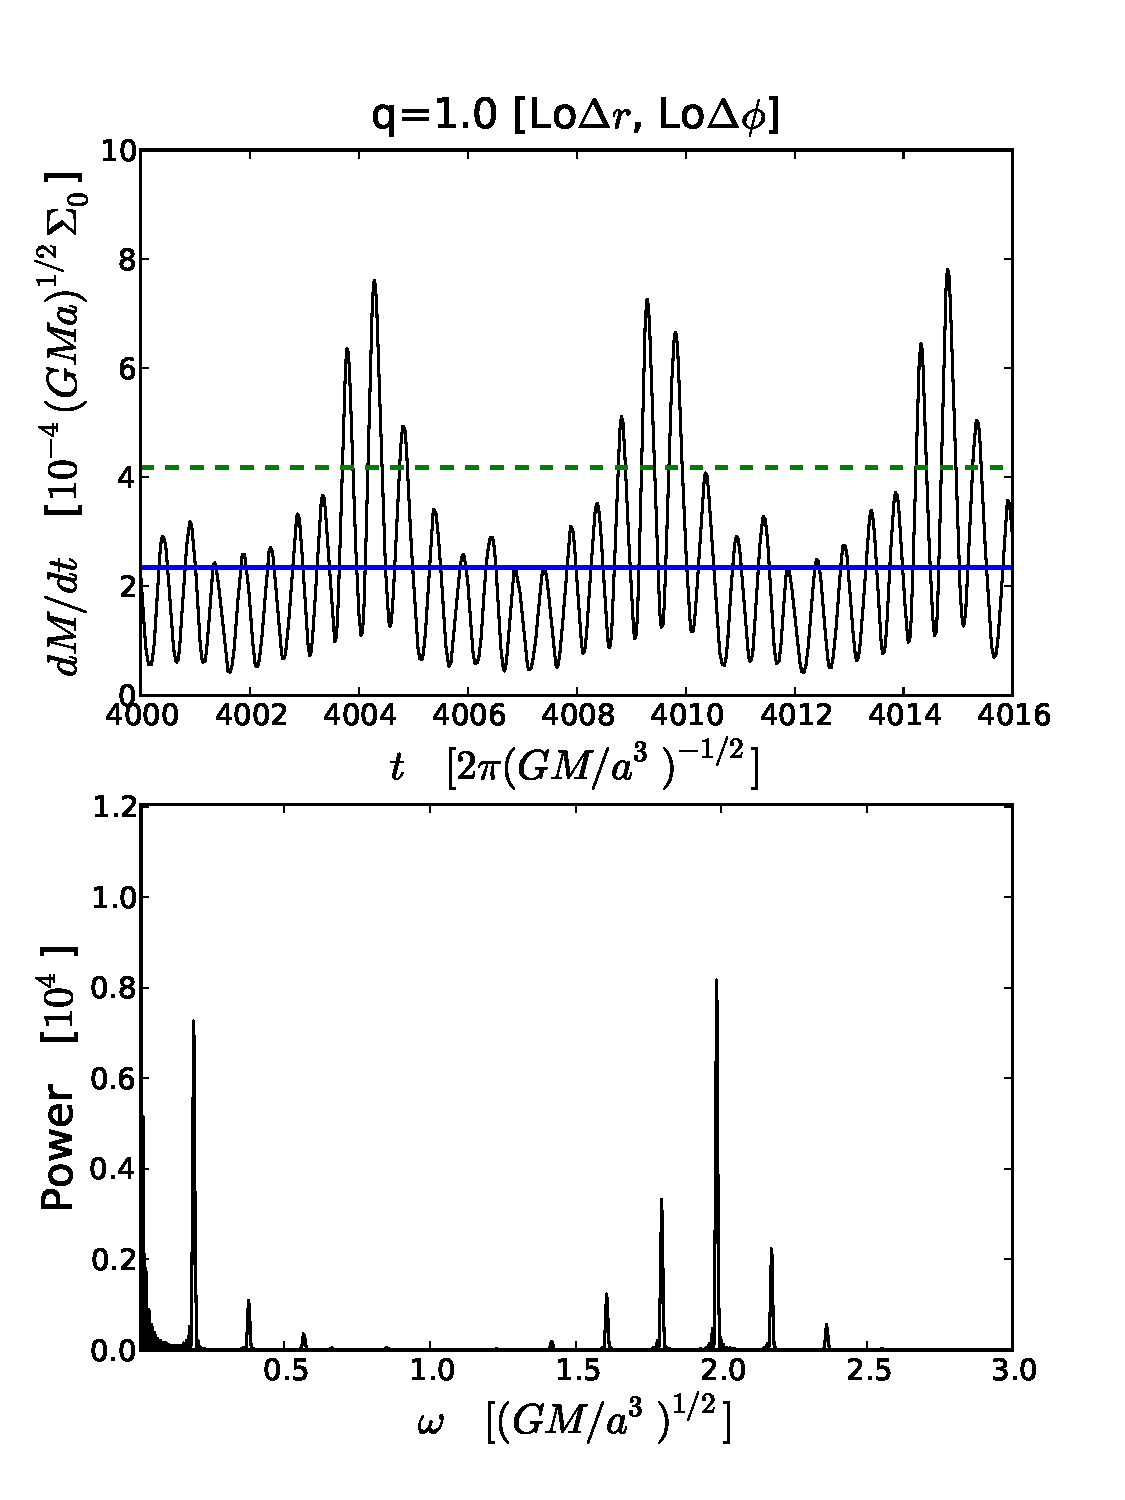
\includegraphics[scale=0.45]{figures/ch1/Mdot_vs_t_q1_FulVsc_alph01_ResLoLo.pdf}
\end{center}
\caption{Accretion rates at the inner boundary $r_{\rm min}=a$ for the
  equal-mass binary as in the top left panels of Figure \ref{Mdott6},
  except for the lowest resolution runs used in this study which 
  matches the highest resolution used in the disc simulated by MM08.  
  The solid horizontal [blue] line in the top panel is the average 
  accretion rate, and the bottom panel shows
  the Lomb-Scargle periodogram computed over 100 binary orbits.} 
\label{MM08_compare}
\end{figure}




\subsection{Viscosity Study}
\label{Viscosity Study}
%
%
%%%%%%%%%%%%%%%%%%%%%%%%%%%%%%%%%%%%%%%
%%% MidLo Res q=1, viscosity
\begin{figure}
\begin{center}$
\begin{array}{cc}
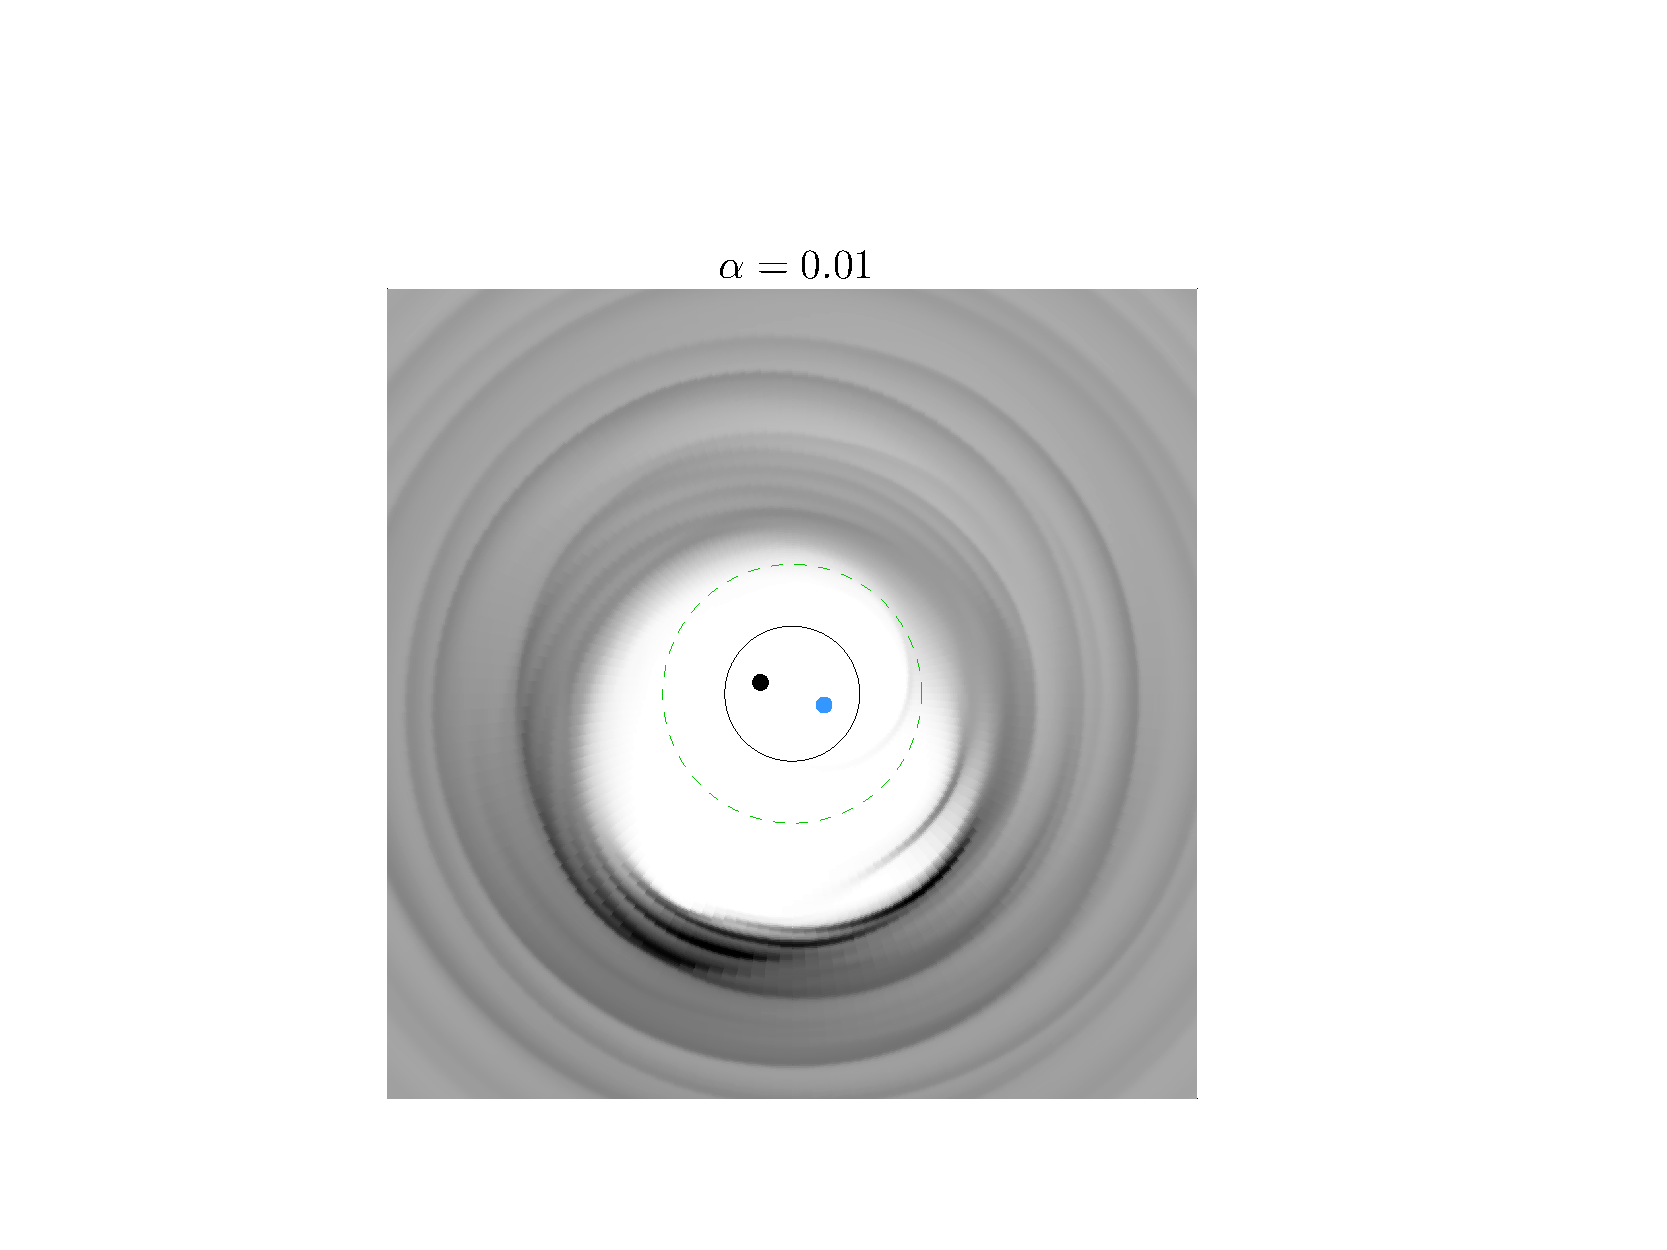
\includegraphics[scale=0.29]{figures/ch1/2DDens_q1_Danvisc_MM_a01_M1G_100a_r24y78_alphFIG_4000} &
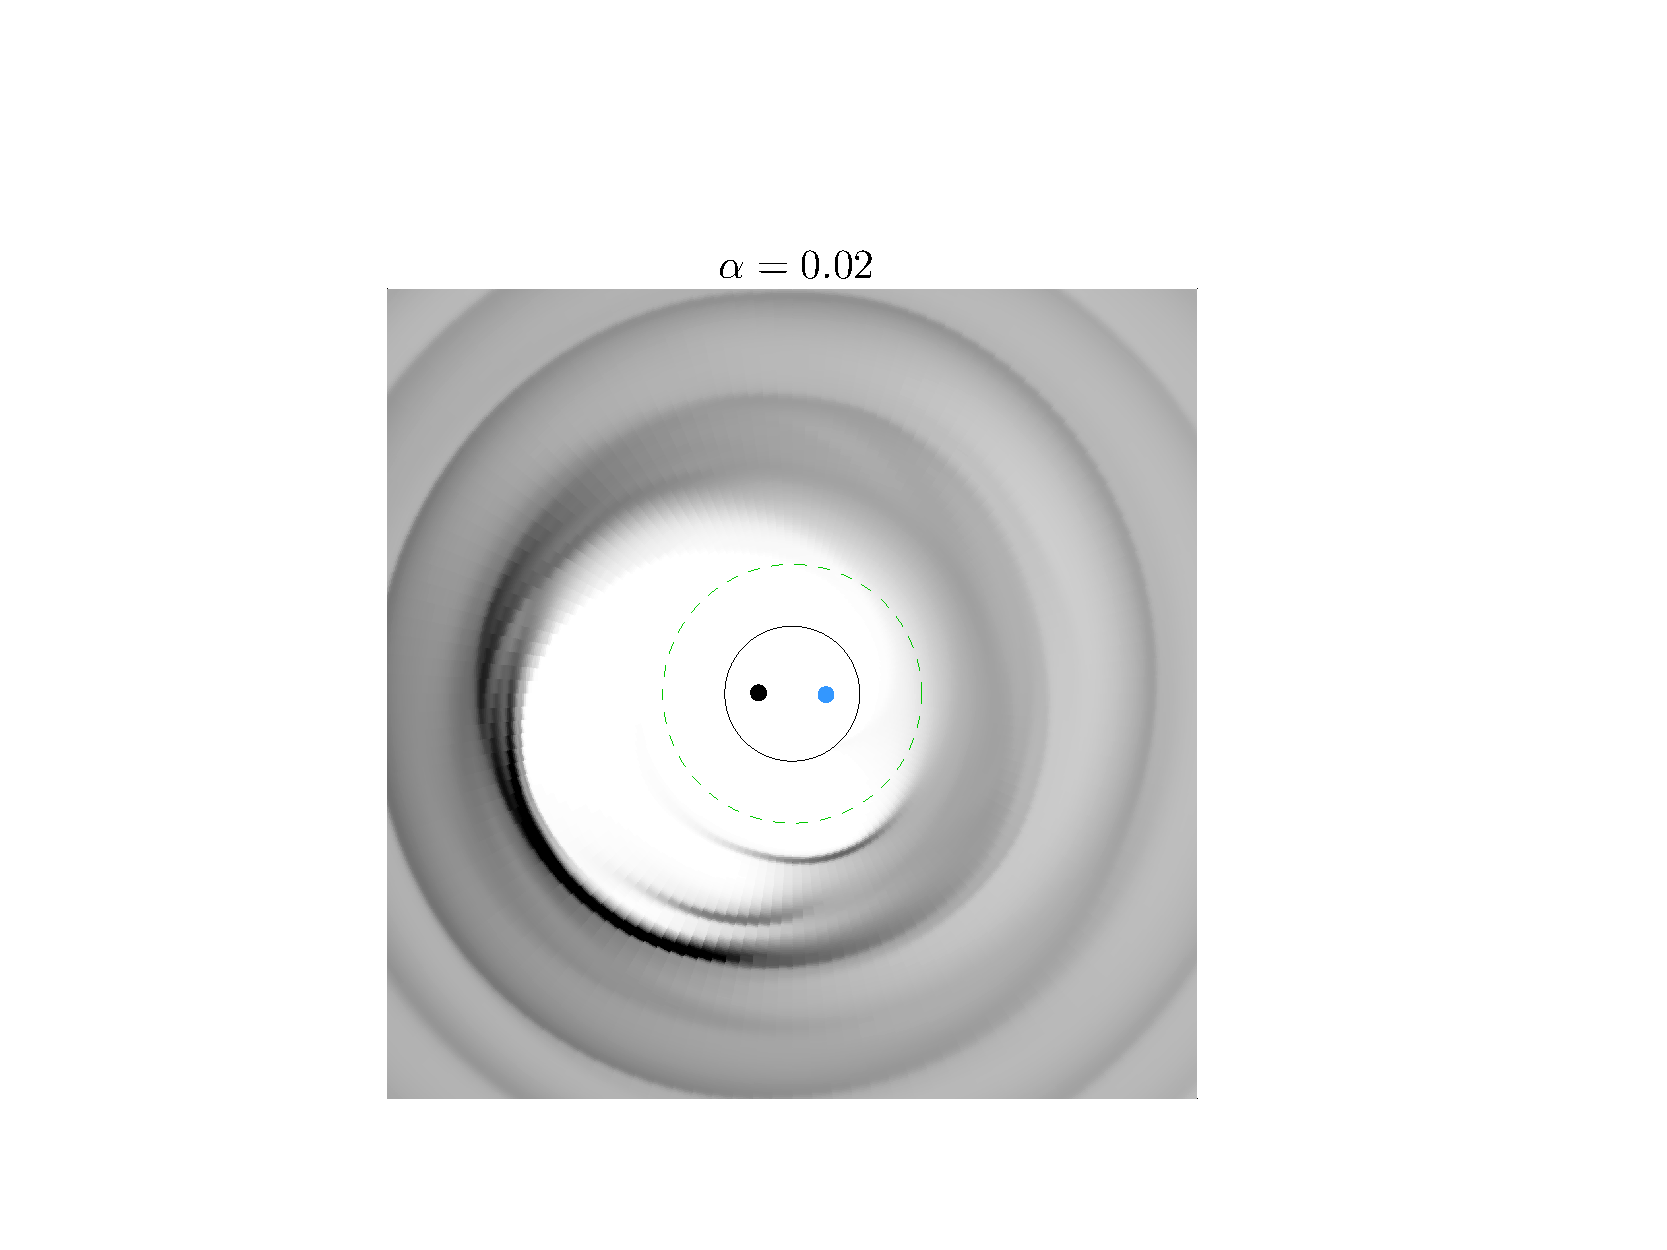
\includegraphics[scale=0.29]{figures/ch1/2DDens_q1_Danvisc_MM_a02_M1G_100a_r24y78_FIG_4000} \\
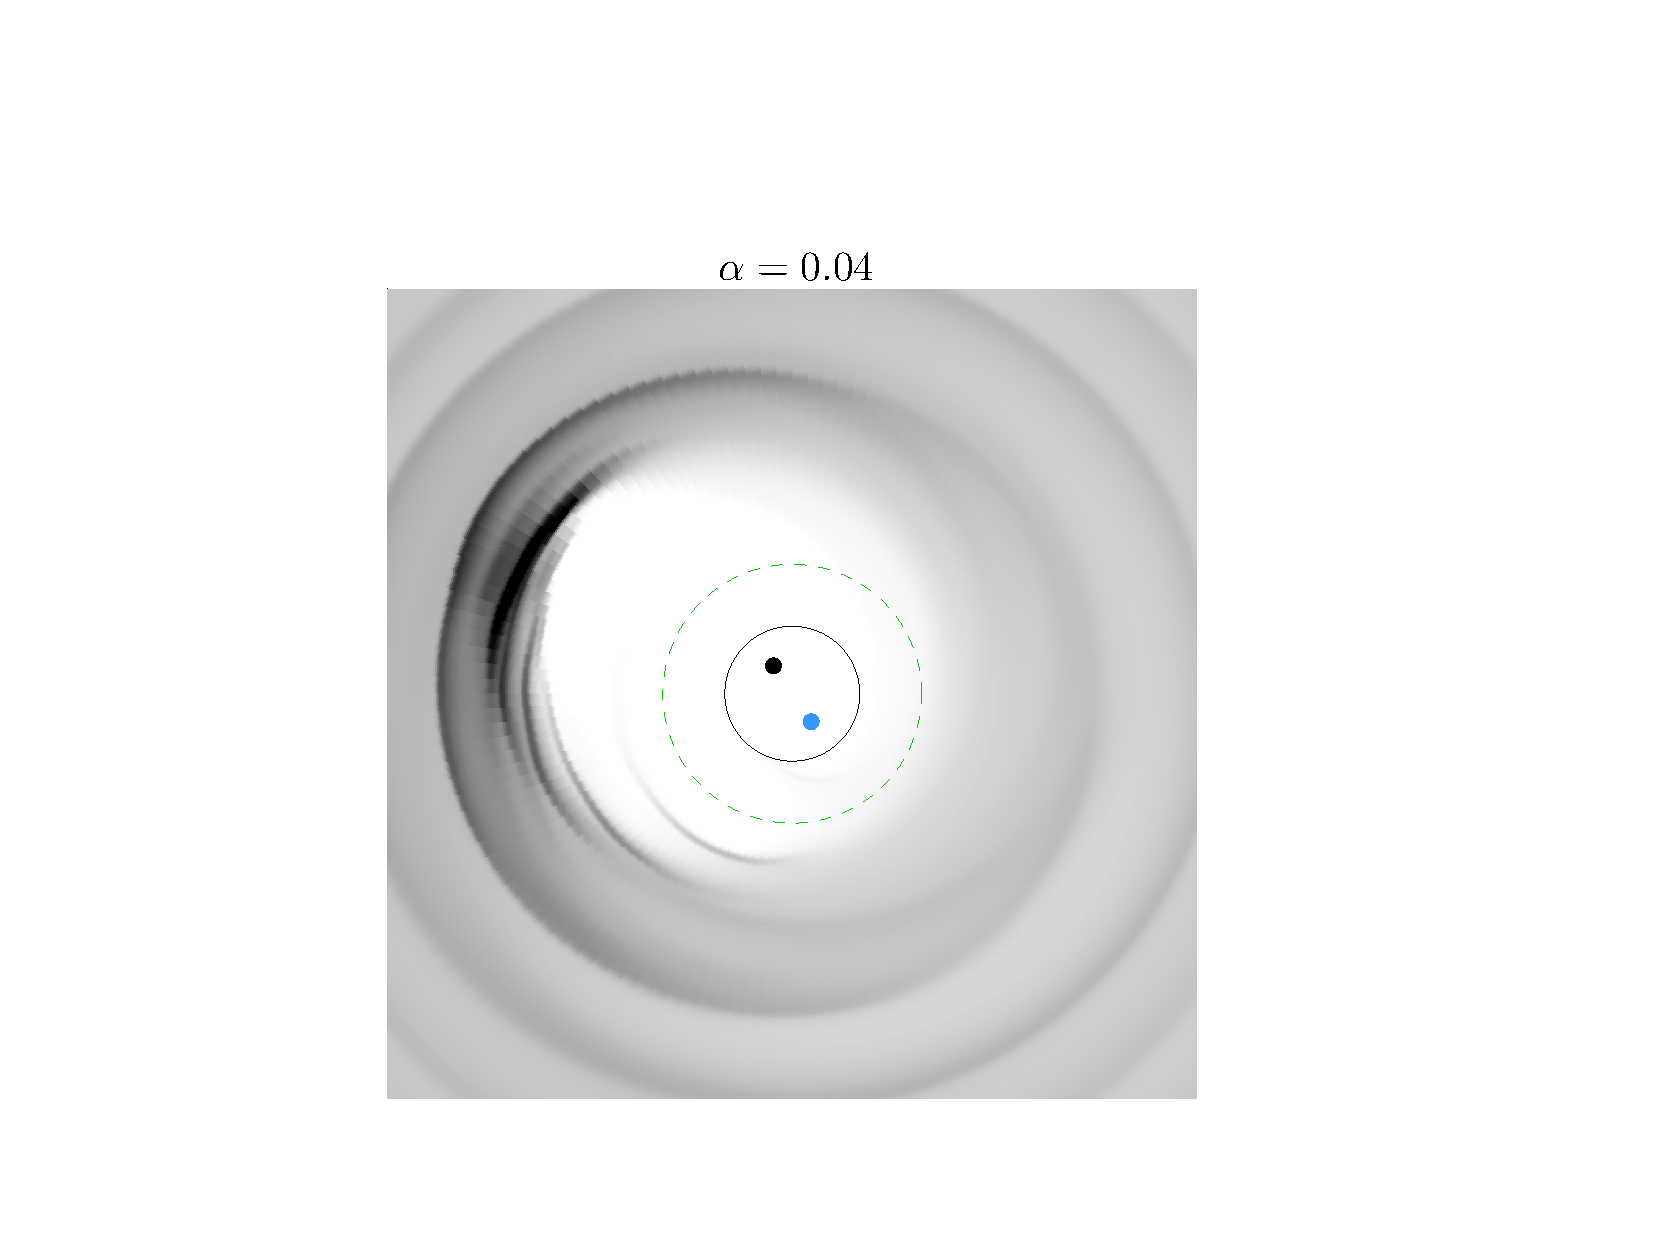
\includegraphics[scale=0.29]{figures/ch1/2DDens_q1_Danvisc_MM_a04_M1G_100a_r24y78_FIG_4002} &
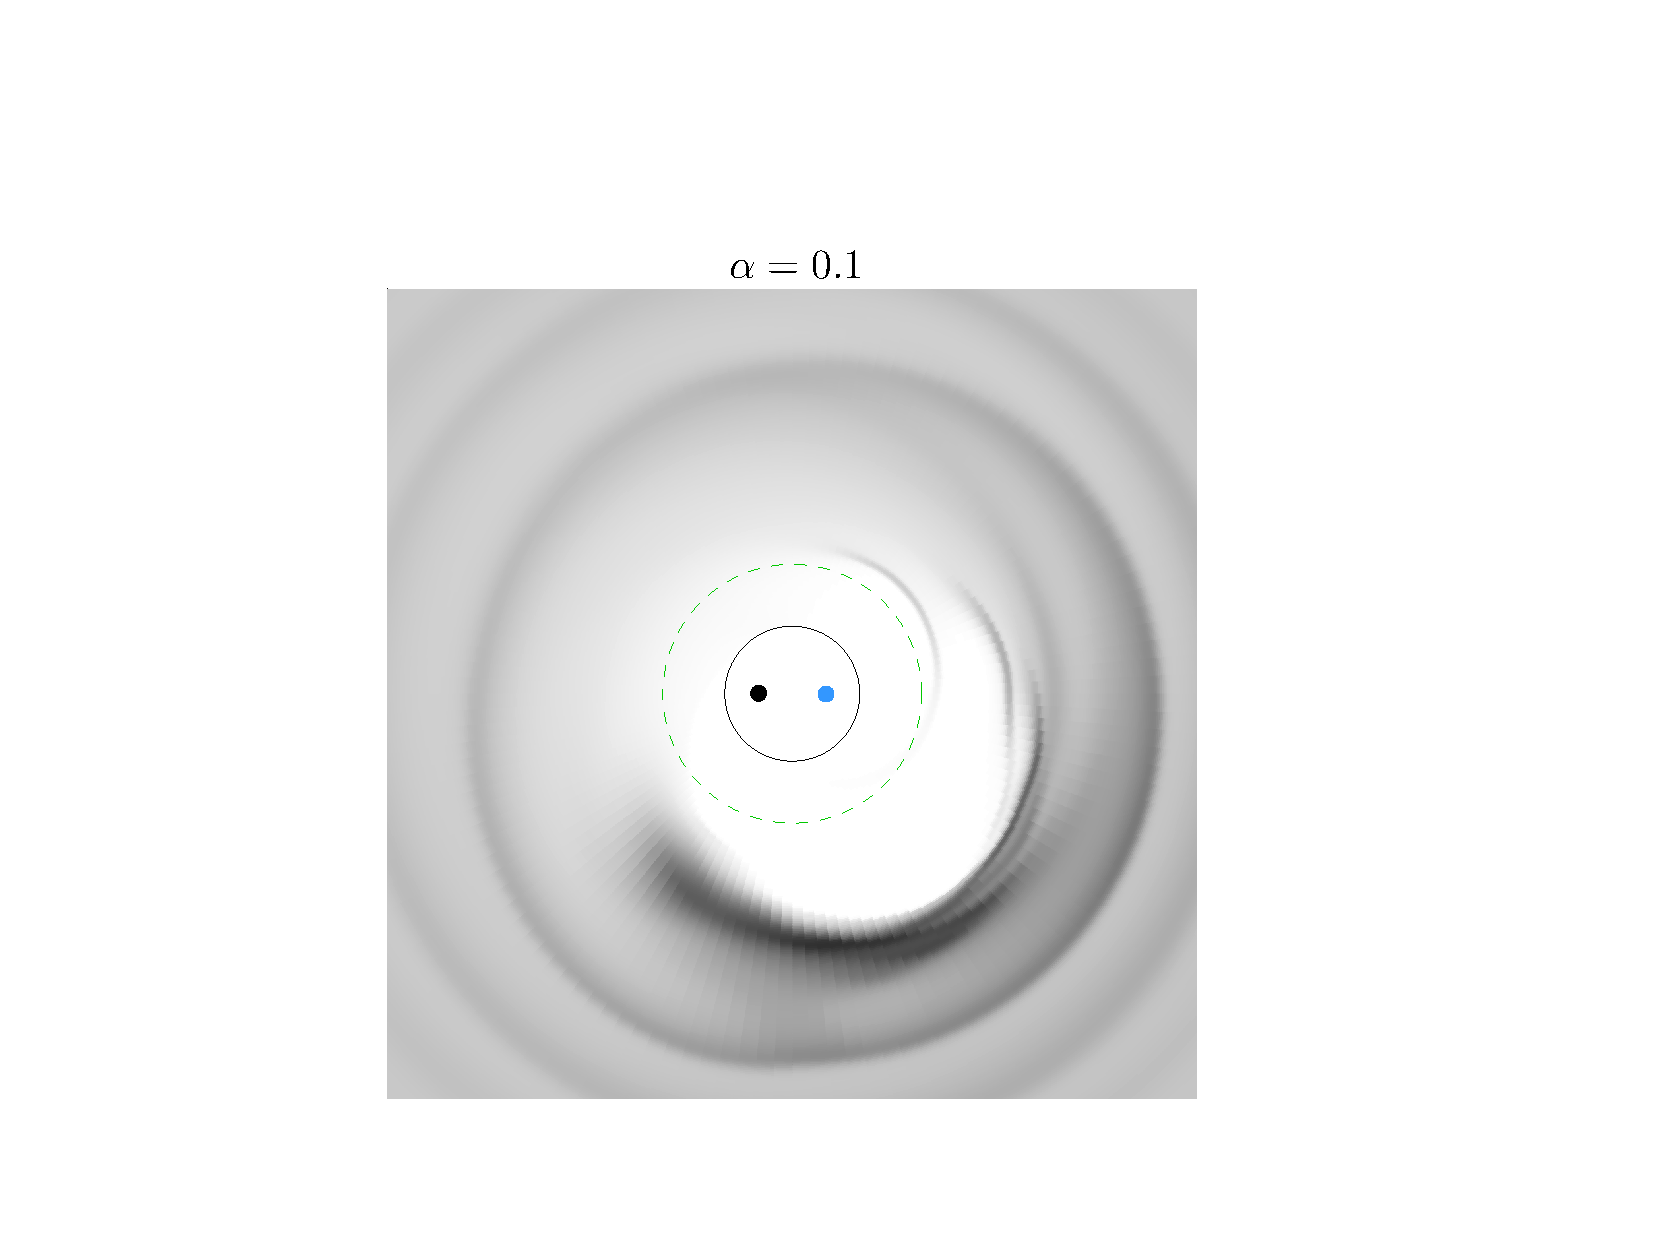
\includegraphics[scale=0.29]{figures/ch1/2DDens_q1_Danvisc_MM_a1_M1G_100a_r24y78_FIG_4000} 
\end{array}$
\end{center}
\caption{Two-dimensional surface density distributions during the quasi steady-state phase,
  as in Figure~\ref{2DDensProf}, except for the single mass ratio
  $q=1.0$, and for four different values of the viscosity parameter $\alpha$, as labeled.  
  Increasing $\alpha$ causes ripples created by streams impacting the cavity wall to smear out more quickly causing the surface density snapshots to appear smoother. For all values of $\alpha$ shown here, the over dense lump still survives long enough to create the $\sim (5-6)t_{\rm bin}$ modulation of the accretion rate. Also for larger $\alpha$, the near side of the disc extends in closer to the binary causing a larger fraction of streams to exit the integration domain at $r=a$. This results in higher measured accretion rates relative to the point mass values for the same $\alpha$'s.}
 \label{Fig:2DDensVsc}
\end{figure}
%%%%%%%%%%%%%%%%%%%%%%%%%%%%%%%%%%%%%%%
%
%
%
%
%%%%%%%%%%%%%%%%%%%%%%%%%%%%%%%%%%%%%%%
%%% alpha all t
\begin{figure*}
\begin{center}$
\begin{array}{cc}
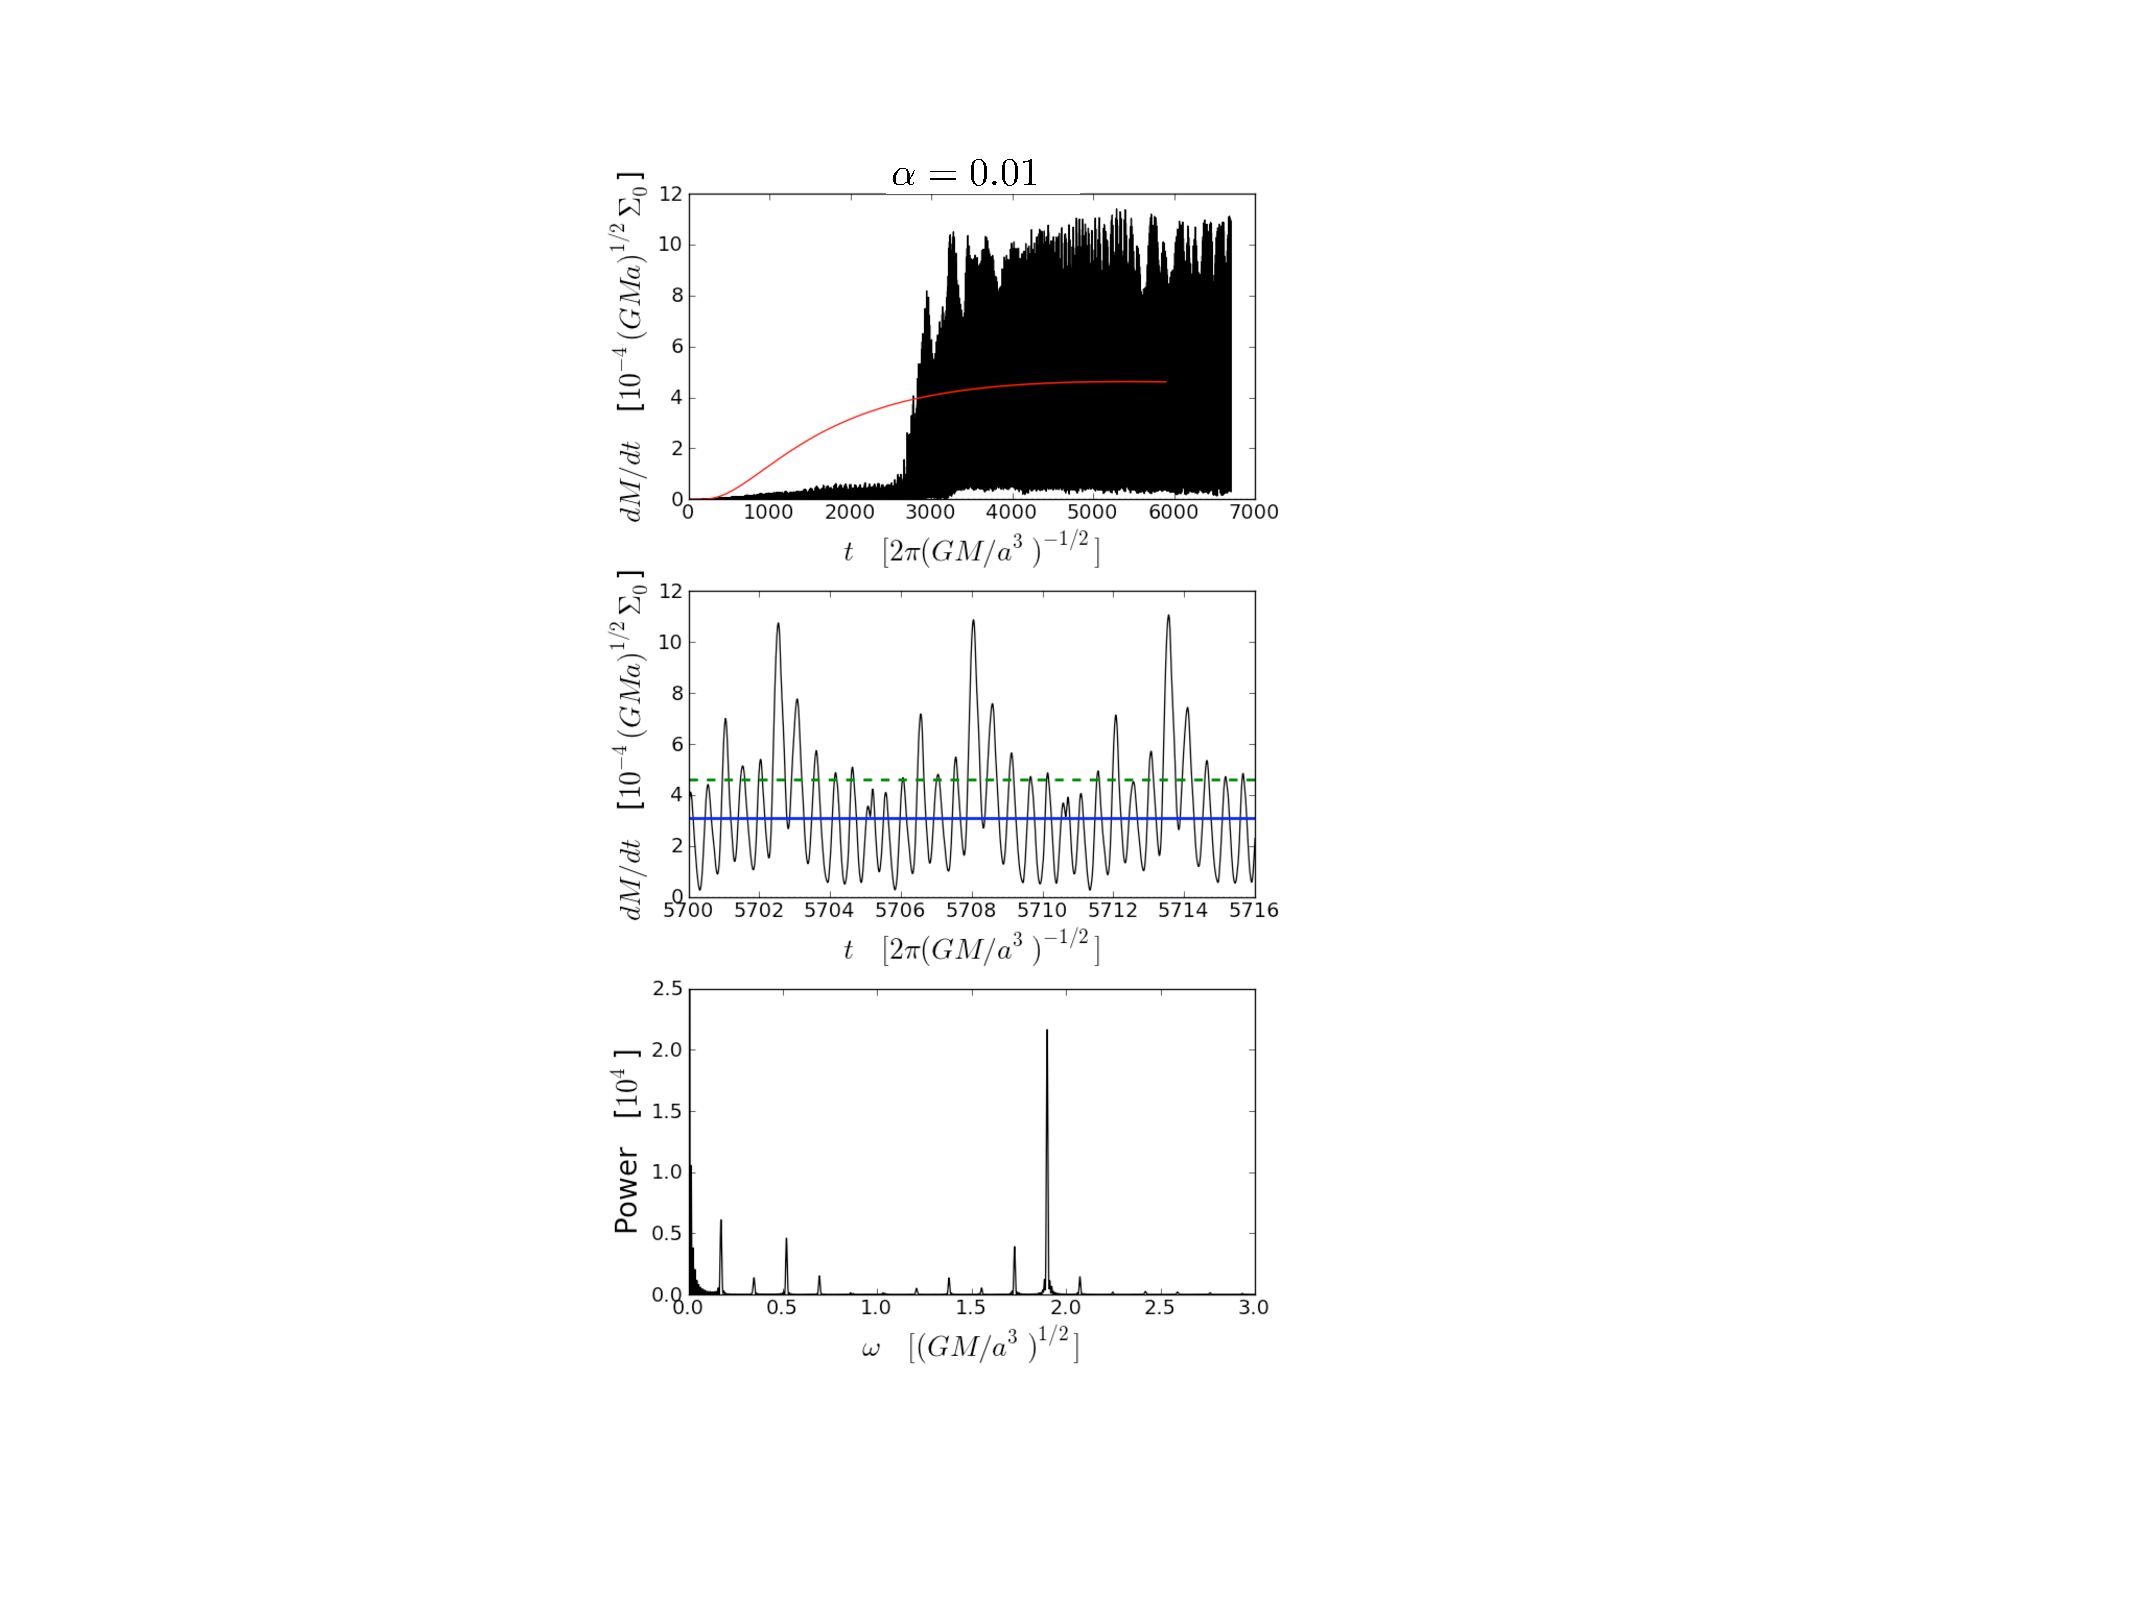
\includegraphics[scale=0.45]{figures/ch1/Mdot_vs_t_q1_FulVsc_alph01_ResMidLo_ALLt_FIG9.pdf} &
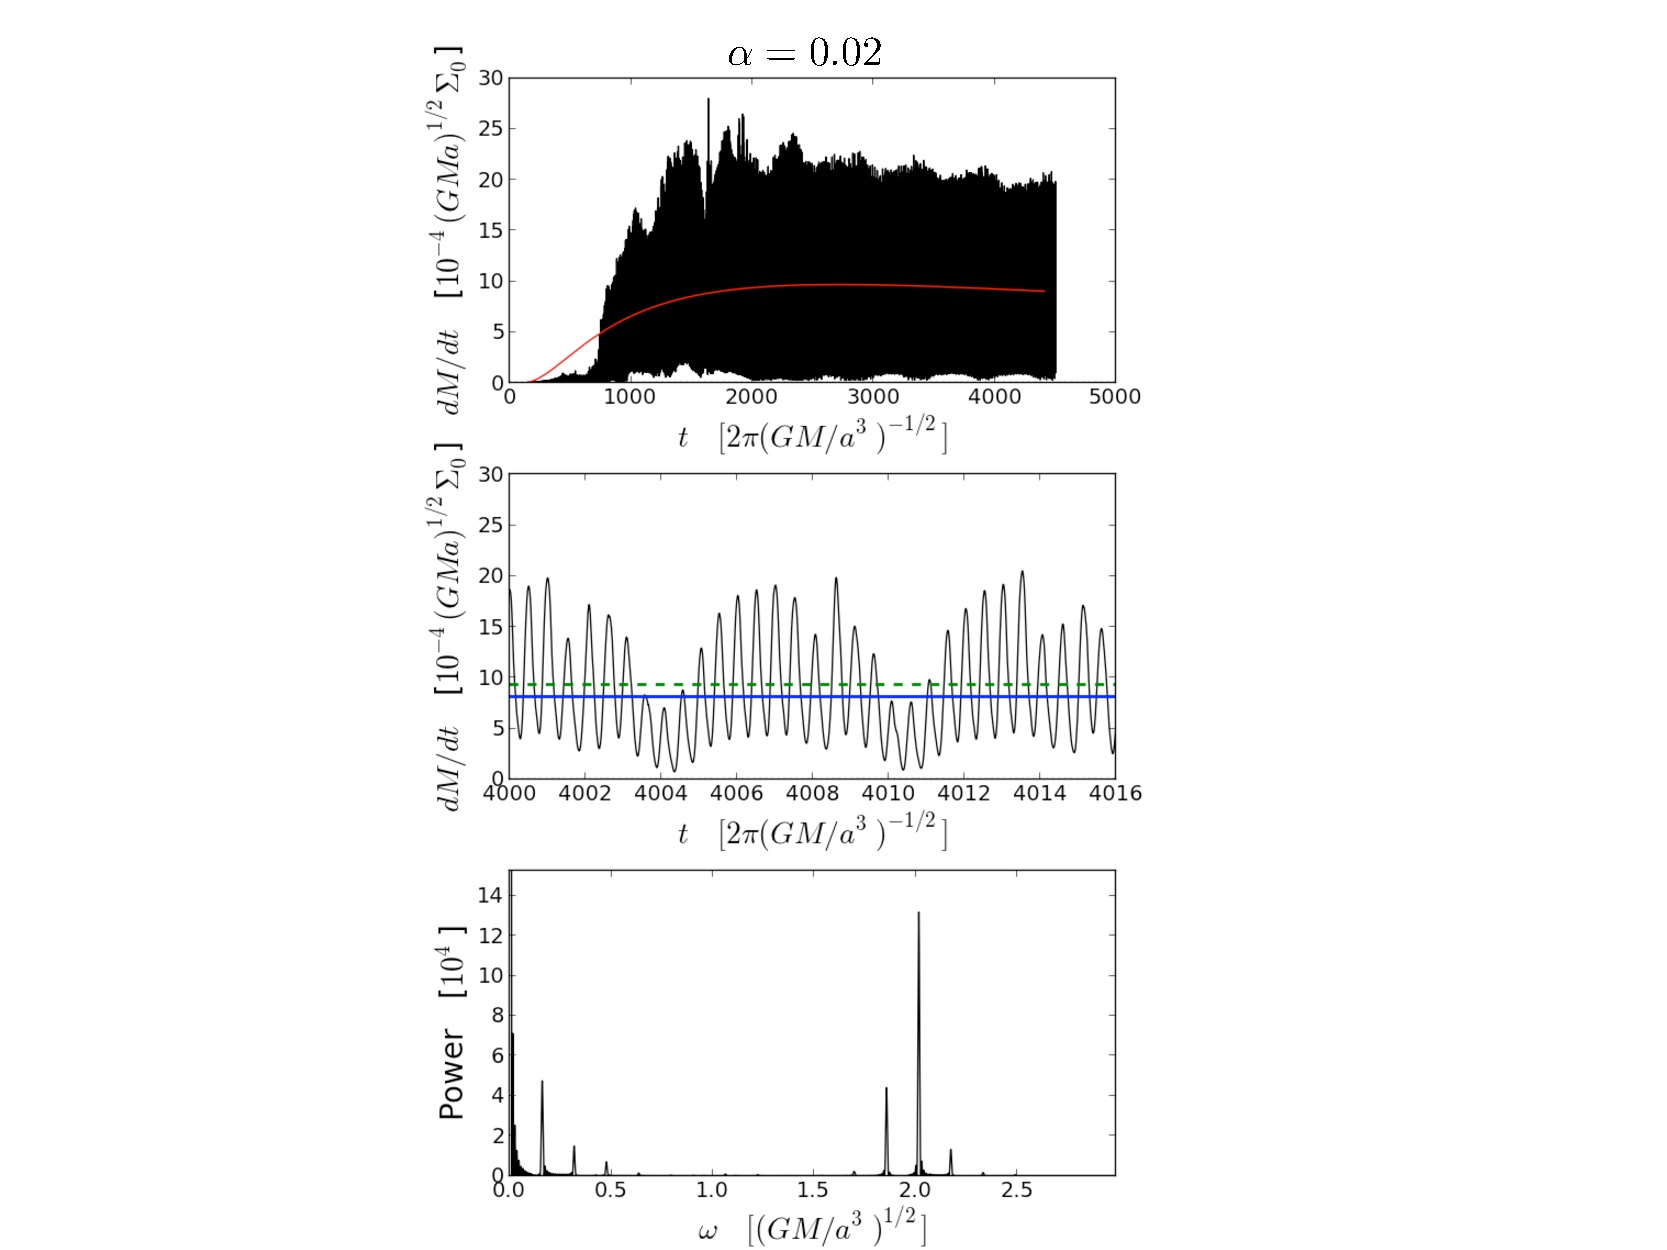
\includegraphics[scale=0.45]{figures/ch1/Mdot_vs_t_q1_FulVsc_alph02_ResMidLo_ALLt_FIG9.pdf} \\
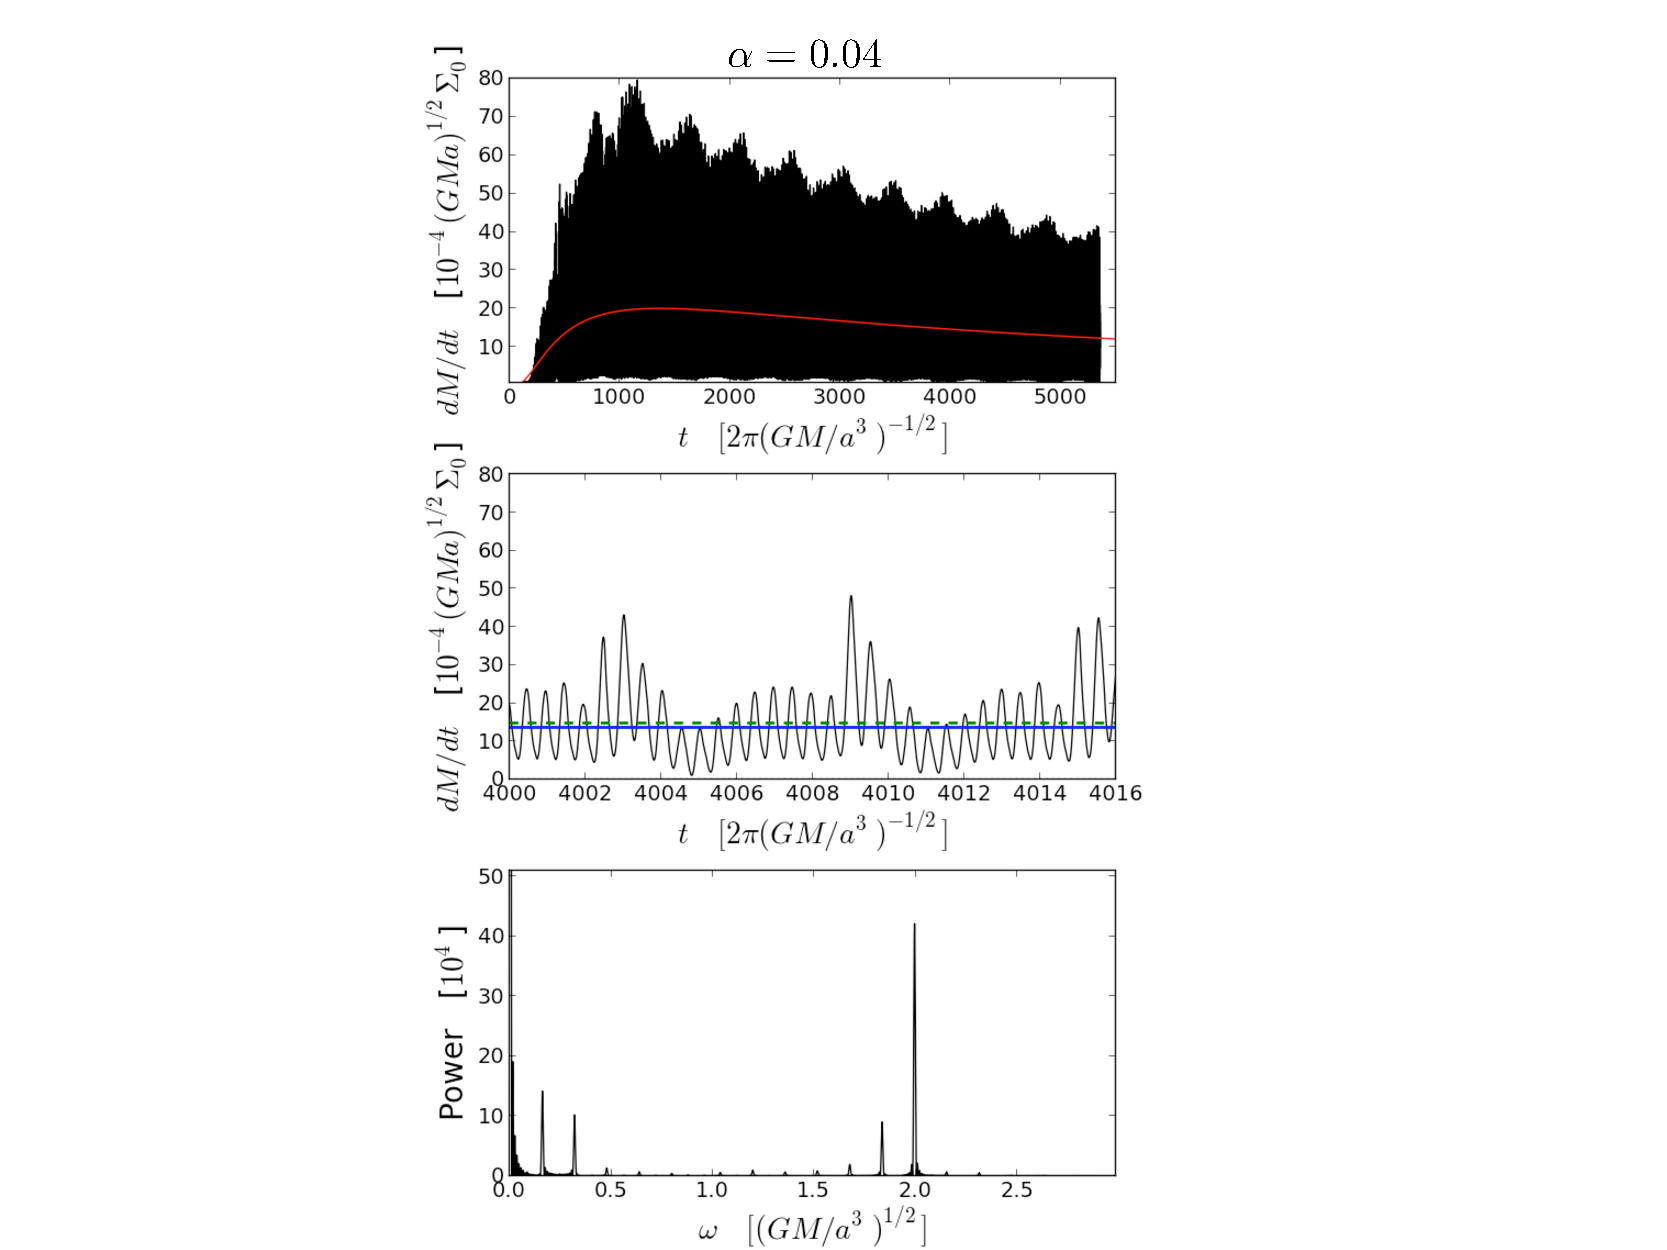
\includegraphics[scale=0.45]{figures/ch1/Mdot_vs_t_q1_FulVsc_alph04_ResMidLo_ALLt_FIG9.pdf} &
\includegraphics[scale=0.45]{figures/ch1/Mdot_vs_t_q1_FulVsc_alph1_ResMidLo_ALLt_FIG9.pdf}
\end{array}$
\end{center}
\caption{The time-dependent accretion rates as in Figure \ref{Mdott6},
  except for the single mass ratio $q=1.0$ and four different
 values of the viscosity parameter $\alpha$, as shown in Figure \ref{Fig:2DDensVsc}. Additionally the top panel of each figure shows the entire accretion rate history for the $q=1$ (black) and $q=0$ (red) cases. Notice that long-term (once per $\sim 400t_{\rm bin}$) variability appears in the larger $\alpha$ runs and is coincident with the period at which the elongated cavity precesses..}
  \label{Fig:Mdott_Vsc}
\end{figure*}
%%%%%%%%%%%%%%%%%%%%%%%%%%%%%%%%%%%%%%%
%
%
To evaluate the sensitivity of our results to the magnitude of viscosity, we run three additional equal-mass binary simulations for $\alpha=0.02$, $0.04$, and $0.1$. Figure \ref{Fig:2DDensVsc} plots snapshots of the 2D surface densities and Figure \ref{Fig:Mdott_Vsc} plots the accretion rates with corresponding periodograms for each of these runs once they have reached the quasi-steady-state regime. Table \ref{Mdot_ratios} records the average accretion rates as a fraction of the reference $q=0$ simulations (a new reference simulation is created for each $\alpha$). Our findings can be summarized as follows:
\begin{enumerate}
	\item{As $\alpha$ is increased, the near side of cavity spreads closer to the binary, as a result, larger portions of streams leave the simulation domain at $r=a$. This results in, not only a larger absolute 	accretion rate, but also an increased rate measured relative to the $q=0$ rate with the same $\alpha$ (See Table \ref{Mdot_ratios}).}
	\item{Despite the increase in average accretion rate, the ratio of maximum accretion rate spikes to the average accretion rate stays constant at $\sim 3$.}
	\item{A transition from a symmetric state to an elongated quasi-steady-state still occurs resulting in discs with similar  morphology including cavities which are of the same size and elongation. As can be seen from Figure \ref{Fig:2DDensVsc}, a difference is that density ripples observed in the fiducial $\alpha=0.01$ disc are progressively more smeared out for the higher $\alpha$ runs. This is due to larger viscous shearing forces more quickly diffusing over-densities due to stream impacts.}
	\item{Although there are larger shearing forces smearing out the small scale density structures seen in the fiducial case, the over-dense lump still survives for at least the necessary $\sim (1/2) t_{\rm bin}$ needed to modulate the accretion rate at the cavity wall orbital period. }
	\item{As a result of the above two points, the periodograms in Figure \ref{Fig:Mdott_Vsc} stay largely the same as $\alpha$ increases. If there is a trend, it is that the timescale associated with the orbital period of the over-dense lump at the cavity wall is more prominent for larger $\alpha$. However, it is possible that, for even larger $\alpha$, the over-dense lump could break up before it can seed another lump via stream generation.}	
	\item{For the larger $\alpha$ runs, the top panels of Figure \ref{Fig:Mdott_Vsc} show the appearance of a longer variability timescale with the same period as the lopsided cavity precession - once per $\sim400$ orbits. This variability manifests itself in a modulation of the maximum accretion rate achieved by the largest streams pulled from the cavity edge lump; every $\sim 400$ orbits the largest accretion rate spikes reach $30 \%$ higher above the average than they do $\sim 200$ orbits later. Note that in the fiducial $\alpha$ case, there is a similar long-term variation in the strength of the $5.7 t_{\rm bin}$ modulation, but it occurs more erratically and with approximately half of the total variation.}
	\label{vi}
	\item{Finally, the top panels of Figure \ref{Fig:Mdott_Vsc} also show that the quasi-steady, lop-sided mode occurs much earlier for larger $\alpha$. For the fiducial case the transition takes place after $\sim 2500  t_{\rm bin}$, for $\alpha=0.02$ after $	\sim 1000  t_{\rm bin}$ and for larger $\alpha=0.04, 0.1$ after less than a few 100 orbits which is set largely by the time for fluid to diffuse to the inner regions of the disc.}
\end{enumerate}
A more detailed investigation of the effects of viscosity should be carried out in future studies and understood self-consistently from simulations which generate turbulent viscosity via the magnetorotational instability (MRI) (See \citealt{ShiKrolik:2012,Noble+2012}). 



\subsection{Resolution Study}
\label{Resolution Study}
Up to now we have discussed the results from our fiducial set of
medium-radial, low-azimuthal resolution runs ($\left[ \hbox{Mid}
  \Delta r, \hbox{Lo}\Delta \phi\right]$ in Table \ref{runs}).
Ideally, we would repeat these runs at increasingly high radial and
azimuthal resolutions, until the results converge.  Unfortunately,
this is computationally prohibitive, and we instead choose the
following approach.

\begin{enumerate}
%
\item For the $q=1.0$ case, we perform two higher-resolution
  runs ($\left[ \hbox{Mid} \Delta r, \hbox{Mid}\Delta \phi \right]$
  and $\left[ \hbox{Hi} \Delta r, \hbox{Hi} \Delta \phi \right]$ in
  Table \ref{runs}) and one lower resolution run ($\left[ \hbox{Lo}
    \Delta r, \hbox{Lo} \Delta \phi \right]$ in Table \ref{runs}) to
  look for signs of convergence.
%
\item We then explore the resolution sensitivity of the boundaries between each accretion regime: The $q=0.1$ case is at the cusp of
  the three--timescale and single--timescale regimes, where we expect the
  accretion behaviour to be particularly sensitive to $q$. The $q=0.05$ case is at the cusp of
  the single--timescale and steady accretion regimes, where the
  minimum accretion rates are achieved. Thus we also run the $q=0.1$ and $q=0.05$ cases for the same set of resolutions as the $q=1$ case. 
  %
\item We repeated each of our runs at the lowest resolution.  Redoing
  the entire set of runs allows us to assess whether different massratios
  are affected by resolution differently.  
\end{enumerate}


%%%q=0.1 Resolution 2DDens
%\begin{figure*}
\begin{figure}
\begin{center}$
\begin{array}{cc}
\includegraphics[scale=0.29]{figures/ch1/2DDens_q01_Danvisc_MM_a01_M1G_100a_r35y78_FIG_4000.pdf} &
\includegraphics[scale=0.29]{figures/ch1/2DDens_q01_Danvisc_MM_a01_M1G_100a_r24y78_FIG_4014.pdf} \\
\includegraphics[scale=0.29]{figures/ch1/2DDens_q01_Danvisc_MM_a01_M1G_100a_r24y52_FIG_4000.pdf} &
\includegraphics[scale=0.29]{figures/ch1/2DDens_q01_Danvisc_MM_a01_M1G_100a_r17y39_FIG_4000.pdf} 
\end{array}$
\end{center}
\caption{Two-dimensional surface density distributions during the quasi steady-state phase,
  as in Figure~\ref{2DDensProf}, except for the single mass ratio
  $q=0.1$, and for four different combinations of high/low radial and
  azimuthal resolutions, as labeled.  Increasing the spatial
  resolution decreases numerical diffusion, leads to sharper features,
  and allows stronger accretion streams.  The stronger streams lead to
  more over-dense lumps where the regurgitated streams hit the cavity
  wall.  As a result, the cavity becomes larger and more lopsided as
  the resolution is increased. In the lowest resolution case, the cavity never becomes lopsided.}
\label{q012DDensRes}
\end{figure}
%\end{figure*}



Figure~\ref{q012DDensRes} gives a visual impression of the surface
density distribution at the four different combinations of resolutions
for $q=0.1$.  They show a clear
trend: as the resolution is increased, the lumps near the cavity wall
become sharper and more over-dense, and the cavity becomes larger and
more lopsided.\footnote{Figure~\ref{RCE} shows that the {\em average}
  position of the cavity wall, found from the azimuthally averaged
  torques in equation (\ref{TrqBalRCE}), is much less affected over
  the range of resolutions studied here.}  This trend can be
attributed to numerical dissipation which is most prominent at shocks, \textit{i.e.} where regurgitated streams
impact the cavity wall.  Increasing the resolution implies weaker
numerical diffusion, stronger accretion streams, more momentum
carried by these streams into the disc, and an overall more efficient driving of the
$m=1$ mode. 
This is further evidenced by an earlier onset of the elongated mode for the higher resolution $q=0.1$ simulations. The $q=0.1$ simulations develop an elongated cavity after $\sim 1500$ (highest resolution), $\sim 2500$ (medium resolution), and $\sim 3500$ (fiducial resolution) binary orbits. The lowest resolution run never develops an elongated cavity even after $\sim 7000$ binary orbits. 

The 2D surface density profiles for the $q=1.0$ runs at different resolutions remain qualitatively the same as the fiducial resolution counterpart. We do find that as the azimuthal  resolution is increased the cavity becomes slightly more elongated likely due again to more efficient stream impacts.

The 2D surface density profiles for the $q=0.05$ runs at different resolutions remain qualitatively the same for all resolutions except the highest resolution. For the highest resolution $q=0.05$ run, the disc transitions in to the single timescale regime only after $\sim 4000$ binary orbits and resembles the $q=0.075$ disc at the fiducial resolution.


%%%q=0.1 Resolution Mdot
\begin{figure*}
%\begin{figure}
\begin{center}$
\begin{array}{cc}
\includegraphics[scale=0.43]{figures/ch1/Mdot_vs_t_q01_FulVsc_alph01_ResLoLo.pdf}&
\includegraphics[scale=0.43]{figures/ch1/Mdot_vs_t_q01_FulVsc_alph01_ResMidLo.pdf} \\
\includegraphics[scale=0.43]{figures/ch1/Mdot_vs_t_q01_FulVsc_alph01_ResMidMid.pdf} &
\includegraphics[scale=0.43]{figures/ch1/Mdot_vs_t_q01_FulVsc_alph01_ResHiHi.pdf}
\end{array}$
\end{center}
\caption{The time-dependent accretion rates as in Figure \ref{Mdott6},
  except for the single mass ratio $q=0.1$ and the four different
  resolutions also shown in Figure \ref{q012DDensRes}. The $q=0.1$
  binary is at the cusp of the transition from the three-timescale to
  the single-timescale regime, and is particularly sensitive to
  resolution, as seen especially in the maxima of the accretion
  spikes.}
\label{q01Res}
%\end{figure}
\end{figure*}

Figure~\ref{q01Res} shows the corresponding time-dependent accretion
rates at the inner boundary of the $q=0.1$ simulations at different resolutions. The accretion patterns
look visibly different for the lowest resolution run which, for reasons stated above never excites the lopsided cavity mode. 
However, encouragingly, the difference between our
fiducial [Mid$\Delta r$,Lo$\Delta \phi$] and the highest-resolution
[Hi$\Delta r$, Hi$\Delta\phi$] cases is modest with a primary trend of increasing accretion rate relative to the $q=0$ rate, with increasing resolution (see Fig.~\ref{Mdot_ratios_plot} and
Table~\ref{Mdot_ratios}).


The accretion rates for the $q=1.0$ runs at different resolutions remain qualitatively the same as their fiducial resolution counterparts. One difference is that the higher and lower (Figure \ref{MM08_compare}) resolution $q=1.0$ runs have more power at the cavity wall periodicity than the fiducial run; the highest resolution run having more power at the cavity wall frequency than at the $2 t_{\rm bin}$ frequency. 
Also, the cavity wall period becomes slightly longer as the resolution increases, from $5.3 t_{\rm bin}$ to $5.7 t_{\rm bin}$ to $5.9 t_{\rm bin}$, to $6.4 t_{\rm bin}$ for the  [Lo$\Delta r$,Lo$\Delta \phi$],  [Mid$\Delta r$,Lo$\Delta \phi$], [Mid$\Delta r$,Mid$\Delta \phi$], and [Hi$\Delta r$,Hi$\Delta \phi$]  runs respectively. A larger cavity again indicates that higher resolution allows more efficient elongation of the cavity. 
This is further evidenced by an earlier onset of the elongated mode for the higher resolution $q=1$ simulations. The two highest resolution $q=1$ simulations develop an elongated cavity at $\sim 1500$ binary orbits where as the two lower resolution runs develop the elongated cavity only after $\sim 2500$ binary orbits.


The accretion rates for the $q=0.05$ runs at different resolutions again remain nearly identical for all resolutions except the highest resolution. For the highest resolution $q=0.05$ run, the disc transitions in to the single, orbital-timescale regime after $\sim 4000$ binary orbits and exhibits modulation of the accretion rate at the orbital frequency, mimicking the $q=0.075$ accretion rates at the fiducial resolution.




Table~\ref{Mdot_ratios} and the corresponding
Figure~\ref{Mdot_ratios_plot} shows the time-averaged accretion rates
as a function of $q$ at different resolutions.  In all cases, at the
same fixed $q$, we find that increasing resolution produces a higher
accretion rate.  This is consistent with the interpretation above that
higher resolution allows stronger accretion streams.  Interestingly,
we find a strong correlation between the values of $\dot{M}_{\rm
  bin}/\dot{M}_{q0}$ listed in Table~\ref{Mdot_ratios} and the
accretion patterns seen in Figure~\ref{q01Res}: runs at different
resolutions but with similar values of $\dot{M}_{\rm bin}/\dot{M}_{q0}$ 
have very similar accretion patterns (including
the variability and the values of the maxima).  The result of
increasing [decreasing] the resolution can therefore be interpreted as
a shift of the accretion behavior to lower [higher] mass ratios.


Comparing the full set of mass ratio runs for the lowest resolution to the fiducial resolution runs, we observe the same progression of the accretion rate through each of the accretion variability regimes discussed above; a difference being that, as discussed in the previous paragraph, the boundaries between each regime are delineated at larger mass ratios in the lowest resolution runs. We also notice that in the three-timescale regime, there is more power in the periodogram peak associated with the cavity wall orbital period (\textit{e.g.} compare the top left of Figure \ref{Mdott6} with Figure \ref{MM08_compare}). The cavity wall peak still disappears for $q=0.25$ when the stream due to the primary becomes much smaller than the stream due to the secondary and the overlapping of large streams at the cavity wall no longer generates an over-dense lump.



Encouragingly, the two higher resolution runs at $q=1.0$,
also plotted in Figure~\ref{Mdot_ratios_plot}, lie closer to each
other than the two lower resolution runs. Since the resolution steps
are evenly spaced, we consider this evidence that the simulations are
converging monotonically with resolution. Since the $q=0.1$ and 
$q=0.05$ discs are positioned at the boundary of different accretion 
regimes we find a large dependence of disc response and accretion rate on resolution, but with a clear 
trend of increasing resolution moving the boundaries between the 
accretion regimes described in this study to slightly lower values of the binary mass ratio. 




%%%%%%%%%%%%%%%%%%%%%%%%
\subsection{Physical Regime: Black Hole Binary Parameters}
\label{Physical Regime}

The simulations presented above can be scaled, in principle, to any black hole mass
and orbital separation.  In this section, we discuss the physical
scales for which our simulations could be relevant (i.e. physically
viable and observationally interesting). The shaded region in 
Figure \ref{ObsCBD} plots this relevant portion of parameter 
space by imposing the following restrictions.

%%%%%%%%%%%%%%%%%%%%%%%%%%%%%%%%%%%%%
%%% Observable CBD's
\begin{figure*}
\begin{center}$
\begin{array}{cc}
\includegraphics[scale=0.45]{figures/ch1/Observable_CBDs_q1_alph01.pdf}&
\includegraphics[scale=0.45]{figures/ch1/Observable_CBDs_q001_alph01.pdf}  
\end{array}$
\end{center}
\caption{The shaded regions in each panel denote the values of binary total mass $M$ and separation $a$ for which a binary + disc system would be physically viable and observationally interesting as well as meet simulation specific constraints. Blue lines denote contours of binary orbital time (a characteristic variability timescale). Green lines denote contours of binary residence time $t_{\rm{res}}\equiv -a (da/dt)^{-1}$ computed from \citealt{HKM09} for migration of the secondary through a gaseous disc as well as gravitational radiation. Dashed black lines denote the simulation specific constraint  that the binary separation not change appreciably over the course of a simulation time. Red lines denote the boundary between gravitationally stable and unstable disc regions via the Toomre Q parameter. Orange lines denote the boundary between binaries which can maintain a cavity and those which will not (computed via the steady-state solutions given by \citealt{Kocsis+2012b}). The left panel is for an equal-mass ratio binary and the right panel is for a binary with mass ratio $q=0.01$. For both plots we use $\alpha=0.1$. Note that for all mass ratios, the most massive binaries do not fit into a gravitationally stable disc. However, this is determined for an undisturbed $\alpha$-disc surrounding the primary; perturbations due to a large secondary would increase the stability of the disc out to larger radii \citep{HKM09}.
In the $q=0.01$ case, less massive, close binaries do not maintain cavities and do not represent systems which are consistent with the initial conditions adopted in this study.}
\label{ObsCBD}
\end{figure*}
%%%%%%%%%%%%%%%%%%%%%%%%%%%%%%%%%%%



\begin{enumerate}
	\item{$10^5~{\rm M_\odot} \lsim M_p \lsim 10^9~{\rm M_\odot}$. It is not clear whether smaller BHs exist in galactic nuclei, and, in any case,
	the radiation from such a low--mass BHs would likely be too faint to
	detect.  Likewise, much more massive BHs are known to be rare.} 
%
	\item{$10^{-2}\lsim q \leq 1$. As we have shown, for the set-up we study (i.e. with a cavity inserted
	by hand into the disc), the accretion pattern converges as we decrease
	the mass ratio to $q=0.01$ and below. In practice, a physical lower limit of $q\sim
	0.01$ may arise from the fact that bound binary BHs can be
	created only in relatively major mergers. 
	In a minor merger, the smaller satellite galaxy may be tidally stripped
	during the early stages of the merger, decreasing the efficiency of dynamical friction, 
	and aborting subsequent binary formation \citep{Callegari+:2009}.
	%
 	Coupled with the well--established correlations
	between the mass of a MBH and its host galaxy, this suggests that the
	$q$--distribution may not extend to values significantly below $q\sim
	0.01$.  \footnote{In principle, less massive BHs may grow from the
 	 accretion discs around the primary \citep{McKernan+2012}; the
	  long-term evolution of such systems would be worthy of further  study.}
	 Figure \ref{ObsCBD} plots the restriction of $a, M$ parameter space for 
	 these limiting mass ratios $q=1$ (left) and $q=0.01$ (right).}
%
	\item{\textit{The binary is embedded in a thin gaseous disc.} Following a merger of two MBH--harboring galaxies, the MBHs sink to
	the bottom of the new galactic potential via dynamical friction in
	approximately a galactic dynamical timescale
	\citep{Begel:Blan:Rees:1980}. In addition to stellar interactions
	(e.g. \citealt{Preto:2011}), many studies have shown that gas in the
	vicinity of the binary could aid in hardening the binary down to $\ll$
	pc separations \citep[\textit{e.g.}][]
	{Escala:2005,Dotti:2007,Mayer+2007,Lodato:2009,Cuadra:2009,Nixon:2011:LongSim,Chapon+2011}.
	We have assumed that such gas in the vicinity of the binary cools
	efficiently and forms a rotationally supported thin disc.  For a given
	$M_p$ and $M_s$, we are still free to choose a physical distance for
	the orbital radius $a$, which could correspond to a snapshot of the
	binary anywhere along its orbital decay.  The assumption that the binary is embedded in a thin disc allows us to make the following additional constraints on $a$ given $M$:
%
	\begin{enumerate}
%
		\item{\textit{The accretion disc is gravitationally stable.} Accretion discs become
		self-gravitating, and unstable to fragmentation, beyond a radius of
		order $ \gsim 10^4 (M/10^7 {\rm M_\odot})^{-1} r_S$ (where $r_S$ is
		the Schwarzschild radius; see, e.g., \citealt{Goodman:2003,HKM09} for the formulae used to generate the $Q\leq1$ criteria in Figure \ref{ObsCBD}).
		Since the binary has to fit inside a gravitationally stable disc, this
		puts an upper limit on the orbital separation denoted by the red lines in Figure \ref{ObsCBD}.}
%
		\item{\textit{Variability occurs on an observable timescale.} The binary orbital time is given by
		%
		\begin{equation}
		 t_{\rm bin} = \frac{2\pi}{\Omega} = 0.88\, 
		\left(\frac{M}{10^7{\rm M_\odot}}\right)
		\left(\frac{a}{10^3 r_S}\right)^{3/2}\, {\rm yr}.
		\label{eq:torb}
		\end{equation}
		%
		As we have shown, the accretion rate shows periodicity on a timescale
		of $\sim t_{\rm bin}$.  In a realistic survey, it will be feasible to
		look for periodic variations between $0.1\,{\rm hr} \lsim
		t_{\rm bin} \lsim {\rm few}\, {\rm yr}$ denoted by the solid blue lines in Figure \ref{ObsCBD}.  
		Here the lower limit comes from the integration time required to measure the flux variations for
		MBHBs in the above mass range (for a survey instrument with a
		sensitivity similar to LSST; \citealt{HKM09}), and the upper limit
		comes from the duration of proposed time-domain surveys.  As a guide, 
		the dashed blue lines in Figure \ref{ObsCBD} are contours of constant orbital times drawn at 10 days and 1 year.}
%
		\item{\textit{The binary spends a long time at a given separation.} 
		Assuming that the binary is embedded in a thin disc,
		\citealt{HKM09} compute residence times, $t_{\rm res}\equiv -a
		(da/dt)^{-1}$, as a function of the binary separation $a$, due to 
		migration of the secondary through the disc and due to gravitational wave 
		decay at small enough binary separations. In Figure \ref{ObsCBD} 
		the green lines denote the requirement that $10^5 \leq t_{\rm res} \leq 10^{10}$ years. 
		A residence time of greater than $10^{10}$ years does not on its own exclude a 
		binary system from observation. Nevertheless, we include this limit in order to show 
		which binaries will not merge (due to migration through a gaseous disc) in a 
		Hubble time. Note also that there is a trade-off: a longer residence time is 
		desirable since it increases the probability of finding such a system; however, 
		longer residence times occur at larger separations and longer orbital times, 
		which will make it more difficult to verify any periodic behavior.}
%
		\item {\textit{A cavity is maintained.} For consistency with the initial conditions 
		adopted here, we require that the binary + disc systems
		will indeed form a cavity during earlier stages of
		their evolution. The region of parameter space for which a cavity 
		may be maintained is denoted by the orange lines in Figure \ref{ObsCBD} 
		and is calculated using the {\em steady-state} disc solutions detailed 
		in \cite{Kocsis+2012b}. }
%
		\item{\textit{The orbital separation is fixed.} Throughout our simulations, we fix the binary separation; we
		therefore require that the orbital decay should be slow enough for the
		binary's orbit not to change significantly over a few thousand
		orbits. This is denoted by the dashed black lines in Figure \ref{ObsCBD} 
		which are drawn where $N_{\rm orb} = t_{\rm res}/t_{\rm bin} =10^5$.} 
%
	\end{enumerate}  }
%
	\item{Though not expressed in Figure \ref{ObsCBD}, for our simulations to be self-consistent, we also require $a\gsim 100
	r_S$, since our Newtonian treatment ignores general relativity.
	Furthermore, at approximately the same binary separation, the orbital
	decay of the binary due to gravitational wave emission becomes more
	rapid than the viscous time at the edge of the cavity. As a result,
	the disc decouples from the binary and is `left behind', rendering our
	initial conditions inconsistent in this regime
	(e.g. \citealt{Milos:Phinney:2005}; although see
	\citealt{FarrisGold:2012} and \citealt{Noble+2012} whose MHD
	simulations suggest that the gas can follow the binary down to smaller
	separations).}
	%
\end{enumerate}


\subsection{Caveats}
\label{Caveats}

However instructive, the simulations presented here are still of
course simplified models of a real binary disc system, and it is worth
listing some major caveats.

\begin{enumerate}
\item Our simulations are two dimensional -- we expect that the 3D
  vertical structure could modify the structure of the accretion
  streams, including their $q$-dependence. However, note that \citealt{Roedig:2012} 
  find similar features in the accretion rate periodograms measured from 3D simulations.
  
\item Our discs are assumed to have angular momentum co-aligned with that of the binary (prograde discs). In principle, a random accretion event onto the binary could result in a misaligned disc which will eventually be torqued into co- or counter-alignment with the binary angular momentum \citep{Nixon:2011:Lett}. 

\item Our simple $\alpha$-viscosity prescription may be inaccurate,
  especially in the nearly radial accretion streams. Recent MHD
  simulations in the $q=1$ case find a larger effective $\alpha$
  than the fiducial value adopted here \citep{ShiKrolik:2012, Noble+2012}.  
  It is interesting, however, that our highest $\alpha=0.1$ simulation for 
  an equal mass binary exhibits the same variability as our fiducial case but a larger accretion rate, 
  in agreement with the above mentioned 3D MHD simulations.

\item We assumed a locally isothermal equation of state; more
  realistic equations of state could have an especially large impact
  on the strength and dissipation of shocks at the cavity wall.
  
\item Our initial conditions correspond to an unperturbed,
  near-Keplerian, circular disc, and circular binary orbit, with a
  significant pile-up of gas.  In reality, accretion onto the binary
  could produce significant binary (as well as disc) eccentricity
  \citep[\textit{e.g.}][]{Cuadra:2009, Lodato:2009, RoedigDotti:2011}.
  In this case, the variability we find would most likely have a more
  complex structure \citep[\textit{e.g.}][]{Hayasaki:2007} due to the
  plethora of resonances available in an eccentric binary potential
  \citep[\textit{e.g.}][]{Artymowicz:1994}. 
In a study of circumbinary discs around eccentric binaries (with mass ratio $1/3$), \citealt{RoedigDotti:2011} find similar accretion rate periodograms as in this study; periodogram peaks exist at the orbital frequency, twice the orbital frequency and the cavity wall orbital frequency. They find that an increasingly eccentric binary: (a) increases the size of the cavity and thus decreases the overall magnitude of the accretion rate, (b) enhances power at harmonics of the orbital frequency, and (c) increases power in a peak located at the beat frequency of the orbital frequency and the cavity wall frequency.
%DD Sept 16
\item As previously stressed, these simulations do not allow the binary orbit to evolve in response to forces exerted by the gas disc. When this assumption of a massless disc is lifted, in addition to changes in binary eccentricity and semi-major axis, the binary center of mass could oscillate around the disc center of mass due to the orbiting eccentric disc. For massive discs, the above effects could alter the description of disc evolution, and hence accretion, presented in this zero disc-mass study.
%
\item Although we begin with an ``empty'' cavity, this cavity may 
  overflow already at a large radius \citep{Kocsis+2012b}.
  Future studies should construct a self-consistent initial density
  profile, by evolving the binary's orbit from large radius through
  gap clearing, and thus determining whether a true pile-up occurs.
\item We have ignored the radiation from the gas accreted onto the
  BHs.  Given that we find high accretion rates -- comparable to those
  for a single BH -- the secondary BH can be fed at super-Eddington
  rates, and the flow dynamics can then be strongly affected by the
  radiation.
\item We have not allowed accretion onto the BHs, and have excised the
  inner region $r<a$ from the simulation domain.  This could have an
  impact on the dynamics of the streams that are flung back towards
  the cavity wall, and therefore on the formation of the dense lump,
  the lopsidedness of the cavity, and the variable accretion patterns.
\end{enumerate}

These caveats should all be pursued in future work, to assess the
robustness of our results.  We expect that our main conclusions,
namely that the accretion rate is strongly modulated by the binary,
and that the power-spectrum of the accretion shows distinct periods,
corresponding to the orbital periods of the binary and the gas near
the location of the cavity wall, will be robust to all of the above
caveats.  However, the numerical values, such as the mean accretion
rate, and the critical value of $q$ for the transition between
variable and steady accretion, will likely be affected.



\section{Conclusions}
\label{Conclusions}

We have investigated the response of an accretion disc to an enclosed
binary via two-dimensional, Newtonian, hydrodynamical simulations. As
previous work has shown (\citealt{Artymowicz:1994, Hayasaki:2007};
MM08; \citealt{Cuadra:2009, ShiKrolik:2012, Roedig:2012}), for
non-extreme mass ratios, the binary carves out a cavity in the disc,
but gas still penetrates the cavity in streams which possibly accrete
onto the binary components. Here we have followed up on the work of
MM08 by investigating the nature of this inflow across the
circumbinary cavity, as a function of binary mass ratio $q$.  We have
simulated 10 different mass ratios in the range $0.003 \leq q \leq
1$. This corresponds to the expected range of $q$-values for massive
BH binaries produced in galaxy-galaxy mergers.

We find that while the binary `propellers' are effective at
maintaining a low-density cavity at the center of the disc, they can
not efficiently suppress accretion across the cavity.  
For $q=1$, the average accretion rate is on order of $2/3$ that of a singe BH 
with accretion spikes of $\sim3$ times larger.  As long
as the circumbinary disc is fueled at a near-Eddington rate from large
radius, these binaries could therefore have quasar-like luminosities.
This should facilitate finding counterparts to GW events
\citep{Kocsis+2006}, and should also allow their detection in
electromagnetic surveys \citep{HKM09}. 


We have found that the accretion is not only strong, but can be
strongly variable (by a factor of $\sim3$), with a characteristic $q$-dependent frequency
pattern.  While the accretion for $q<0.05$ is steady, for $q\gsim
0.05$ there is a strong modulation by the binary, and a clear
dependence on $q$ of both the variability pattern, and the magnitude
of the time-averaged accretion rate.  For an equal-mass binary, the
accretion rate is modulated at twice the orbital frequency and $\sim
1/6$ the orbital frequency.  As the mass ratio is lowered, the power
in the $1/2 t_{\rm bin}$ and $(5-6)t_{\rm bin}$ variability timescales is
reduced, and traded for a third variability timescale at $t_{\rm
  bin}$.  In the range $0.05 \lsim q \lsim 0.25$, the single
$t_{\rm bin}$ timescale is dominant.   


Increasing the magnitude of viscous forces has little effect on the above findings except to increase the magnitude of the accretion rate (both absolute and relative to $q=0$) and to bring out a long-term accretion variability timescale with a periodicity of $400 t_{\rm bin}$. However, accretion discs with even larger viscous forces could quench the $(5-6)t_{\rm bin}$ variability timescale if the over-dense lump responsible for its generation can be broken up before it repeats $\sim$ an orbit at the cavity wall. Hence, further investigation into the effects of viscosity are warranted.

Strong and highly variable accretion, with characteristic
frequencies, should aid in identifying massive BH binaries in galactic
nuclei.  The presence of two frequencies, in the ratio 1:2 for unequal-mass binaries ($0.1 \leq q < 1$), is an
especially robust prediction that is {\em independent of disc
  properties}, and could serve as a `smoking gun' evidence for the
presence of a binary.  Our results suggest that the ratio of the power
at these two frequencies could probe the mass ratio $q$, while other
features of the periodogram could probe properties of the disc, such
as its viscosity.


The variability time-scales are on the order of the orbital period,
and we have argued that the most promising candidates in a blind
electromagnetic search would be those with total mass and separation contained in the shaded regions of Figure \ref{ObsCBD}; $10^{6-7} {\rm M_\odot}$ binaries,
preferably with orbital periods of days to weeks.  The time-variable accretion to
the central regions could produce corresponding variability in
broad-band luminosities, allowing a search in a large time-domain
survey, such as LSST, without spectroscopy.  Additionally, the
emission lines could exhibit periodic shifts in both amplitude and
frequency; kinematic effects from the binary's orbit could be
distinguished from those due to the fluctuating accretion rate,
whenever the latter contains multiples of the binary period.

A few percent of the accretion streams generated periodically fuel the BHs,
but the majority of the stream material is flung back and hits the accretion
disc farther out. The shocks produced at these impact sites are
prominent for $q\gsim 0.1$, and can provide additional observable
signatures.  In particular, radiation from these shocks should be
temporally correlated with the luminosity modulations arising near the
secondary and/or primary BH, with a delay time on the order of a
binary orbit.

GW observatories, such as eLISA, and Pulsar Timing Arrays will be able to constrain the mass
ratios of in-spiraling MBHB's at the centers of galactic nuclei
ab-initio, providing a template for the expected variability pattern.
This should be helpful in identifying the unique EM counterpart among
the many candidates (with luminosity variations) in the eLISA/PTA error
box, as the source with a matching period.

In summary, our results imply that massive BH binaries can be both
bright and exhibit strongly luminosity variations, at the factor of
several level. This raises the hopes that they can be identified in a
future, suitably designed electromagnetic survey, based on their
periodic variability.  Although encouraging, these conclusions are
drawn from simplified 2D hydrodynamical models of a real binary disc
system, and should be confirmed in future work.


\section*{Acknowledgments}

We thank Brian Farris and Bence Kocsis for useful discussions.  We thank Paul
Duffell for useful discussions, for verifying some of our results
in independent runs with the code DISCO, and also for suggesting 
the Cartesian shear flow test of our viscosity implementation. We also thank 
the anonymous referee for constructive comments which have improved this manuscript. 
We acknowledge support from NASA grant NNX11AE05G (to ZH and AM). 
DJD acknowledges support by a National Science Foundation Graduate 
Research Fellowship under Grant No. DGE1144155.

%\bibliography{Dan}

%%%%%%%%%%%%%%%%%%%%%%%%%%%%%%%%%%%%%%%%%%%%%
%\appendix
%added for thesis
%\begin{appendix}
%%%%%%%%%%%%%%%%%%%%%%%%%%%%%%%%%%%%%%%%%%%%%
\section{Viscous implementation in polar coordinates}
\subsection{Viscosity and the Momentum Equation}
We may write the momentum equation in component form and with respect to an arbitrary basis as
\begin{equation}
\partial_t(\rho v_i) = -\nabla_j \Pi_{ i}^{\ j}
\label{MvEqn} 
\end{equation}
where $\nabla$ represents the covariant derivative,
\begin{equation}
\Pi_{ij}  = P g_{ij} + \rho v_i v_j - \sigma_{ij}
\label{MvTensor}
\end{equation}
are the components of the momentum flux density vector, P is the mechanical pressure, and $g$ is the metric tensor. The first two terms represent a reversible momentum flux due to pressure forces and mechanical transport of the fluid. The last term expresses a non-reversible momentum flux due to viscous forces via the \textit{viscous stress tensor} $\sigma$. Writing out (\ref{MvEqn}) with (\ref{MvTensor}),
\begin{equation}
\partial_t(\rho v_i) = \nabla_j (P g_{ i}^{\ j} ) +  \nabla_j (\rho v_i v^j - \sigma_{ i}^{\ j} ) \nonumber
\end{equation} 
or in vector notation
\begin{equation}
\partial_t(\rho \mathbf{v}) = -\nabla P -  \nabla \cdot (\rho \mathbf{v v} - \sigma) 
\label{MvVector}
\end{equation} 
Thus we see that the effects of viscosity can be incorporated by computing viscous momentum fluxes from $\sigma$ and subtracting them from the mechanical transport term $\rho \mathbf{v v}$. This is what FLASH does currently to incorporate the effects of viscosity in Cartesian coordinates. However, in non-Cartesian coordinates, there will also be geometric source terms from taking the divergence of the rank-two-tensors $\mathbf{v v}$ and $\sigma$. Thus we must compute not only the components of these terms, but also the divergence in order to identify geometric source terms.

\subsection{The Form of the Viscous Stress Tensor}
The viscous stress tensor has components \citep{LandauLifschitz:Fluids}
\begin{equation}
\sigma_{ij} = \rho \left[ \nu\left(\nabla_i v_j + \nabla_j v_i \right) + \left(\zeta - \frac{2}{D} \nu \right) g_{ij} \nabla_l  v^l   \right]
\label{ViscTensor}
\end{equation}
where $\nu$ is the kinematic coefficient of viscosity, $\zeta$ is the bulk coefficient of viscosity, and D is the number of spatial dimensions. The $2/D$ factor is chosen so that only the bulk viscosity term survives upon taking the trace of $\sigma$. 


\subsection{Components of $\sigma$ in Polar Coordinates}
To compute the viscous stress tensor components we work in a coordinate basis to evaluate the covariant derivatives in terms of Christoffel symbols,
\begin{equation}
\nabla_j T_i = \partial_j T_i - \Gamma^k_{\ ij}T_k \nonumber
\end{equation} 
Working in 2D polar coordinates, $(r, \phi)$, the non-zero Christoffel symbols are
\begin{equation}
 \Gamma^r_{\ \phi \phi} = -r \qquad  \Gamma^{\phi}_{\ r \phi}=\Gamma^{\phi}_{\  \phi r} = \frac{1}{r} \nonumber
\end{equation} 
In the polar coordinate basis Eqs.\ (\ref{ViscTensor}) become
\begin{align}
\sigma_{rr} &= \Sigma \left[ 2 \nu \partial_r v_r + \left( \zeta -1 \right) \nabla \cdot v \right]   \nonumber \\
\sigma_{r \phi} &= \Sigma \left[  \nu \left( \partial_r v_{\phi} + \partial_{\phi}v_r  - \frac{2}{r} v_{\phi} \right) \right] \nonumber \\
\sigma_{\phi \phi} &= \Sigma \left[ 2 \nu \left(\partial_{\phi} v_{\phi} + r v_r \right) + \left( \zeta - 1\right) r^2 \nabla \cdot v \right]  \nonumber 
\end{align}
where $\Sigma$ is the height integrated 2D surface density, $v^{\phi}=\Omega$ and $v_{\phi}= r^2 \Omega$, $\Omega$ being the angular frequency.
Transforming to an orthonormal basis (used in FLASH)
%
\footnote{For this conversion one needs to contract the coordinate tensor components with the orthonormal components of the coordinate basis vectors. This simply amounts to multiplying each $\phi$-up component by $r$ and each $\phi$-down component by $1/r$ (\textit{e.g.} $v^{\hat{\phi}} = r v^{\phi} = v_{\hat{\phi}} = v_{\phi}/r = r \Omega$).}
%
these components become,
\begin{align}
\sigma_{\hr \hr} &= \Sigma \left[ 2 \nu \partial_r v_{\hr} + \left( \zeta -1 \right) \nabla \cdot v \right]  \nonumber \\
r \sigma_{\hr \hp} &= \Sigma \left[  \nu \left( \partial_r \left(r v_{\hp} \right)+ \partial_{\phi}\left(r v_{\hr} \right) - \frac{2}{r}\left( r v_{\hp} \right) \right) \right]  \nonumber \\
r^2 \sigma_{\hp \hp} &=  \Sigma \left[ 2 \nu \left(\partial_{\phi}(r v_{\hp}) + r v_{\hr} \right) + \left( \zeta - 1 \right) r^2 \nabla \cdot v \right]  \nonumber 
\end{align}
where $v^{\hat{\phi}}=\vp= r \Omega$. Since the value of the bulk viscosity coefficient $\zeta$ is somewhat arbitrary, 
we set it to 0. Then simplifying the above using $\nabla \cdot v = \partial_r v_r + \frac{1}{r} \partial_{\phi} v_{\phi} + \frac{v_r}{r}$,
\begin{center}
%\boxed{
%\begin{gathered}
\begin{align}
\sigma_{\hr \hr} = \Sigma \nu \left[  \partial_r \vr -  \frac{1}{r}\partial_{\phi} \vp -  \frac{\vr}{r} \right]  \nonumber \\
\sigma_{\hr \hp} =  \Sigma \nu \left[  \partial_r \vp +  \frac{1}{r}\partial_{\phi} \vr -  \frac{\vp}{r} \right]  \nonumber \\
\sigma_{\hp \hp} = \Sigma \nu \left[   \frac{1}{r}\partial_{\phi} \vp -  \partial_r \vr + \frac{\vr}{r} \right] 
\label{OrthComps}
\end{align}
%\end{gathered}
%}
\end{center}


\subsection{Divergence of $\sigma$ in Polar Coordinates}
To compute the geometric source terms which will modify the 2D polar momentum equation we compute the divergence of the second rank tensor $\sigma$. Starting again in a coordinate bases we may write,
\begin{equation}
\left( \nabla \cdot \sigma \right)^i = \partial_j \sigma^{ji} + \Gamma^j_{\ kj} \sigma^{ki} + \Gamma^i_{\ kj} \sigma^{kj}
\end{equation}
giving us the components of the viscous force
\begin{align}
\left( \nabla \cdot \sigma \right)^r &=  \partial_r \sigma^{rr} + \partial_{\phi} \sigma^{\phi r} + \frac{1}{r}\sigma^{rr} - r\sigma^{\phi \phi} \nonumber \\
\left( \nabla \cdot \sigma \right)^{\phi} &=  \partial_r \sigma^{r\phi} + \partial_{\phi} \sigma^{\phi \phi} + \frac{3}{r}\sigma^{r \phi} \nonumber
\end{align}
Transforming again to an orthonormal basis for implementation in FLASH,
\begin{align}
\left( \nabla \cdot \sigma \right)^{\hr} &=  \partial_r \sigma^{\hr \hr} + \partial_{\phi}  \frac{1}{r}\sigma^{\hp \hr} + \frac{1}{r}\sigma^{\hr \hr} - r \left( \frac{1}{r^2} \sigma^{\hp \hp} \right) \nonumber \\
\frac{1}{r}\left( \nabla \cdot \sigma \right)^{\hp} &=  \partial_r  \left( \frac{1}{r}\sigma^{\hr \hp} \right) + \partial_{\phi}  \frac{1}{r^2} \sigma^{\hp \hp} + \frac{3}{r}  \left( \frac{1}{r} \sigma^{\hr \hp}\right) \nonumber.
\end{align}
Simplifying,
\begin{center}
%\boxed
%\begin{gathered}
\begin{align}
\left( \nabla \cdot \sigma \right)^{\hr} =  \frac{1}{r} \partial_r \left( r \sigma^{\hr \hr} \right) + \frac{1}{r}\partial_{\phi} \left( \sigma^{\hp \hr} \right) - \frac{1}{r} \sigma^{\hp \hp}  \nonumber \\
\left( \nabla \cdot \sigma \right)^{\hp} = \frac{1}{r} \partial_r \left( r \sigma^{\hr \hp} \right) + \frac{1}{r}\partial_{\phi} \left( \sigma^{\hp \hp} \right)+ \frac{1}{r} \sigma^{\hr \hp}    .
\label{NonAngDiv}
\end{align}
%\end{gathered}
%}
\end{center}
Plugging in the values of the components from (\ref{OrthComps}) we have,
\begin{center}
%\boxed{
%\begin{gathered}
\begin{align}
(\nabla \cdot \sigma)_{\hat{r}} = \frac{1}{r} \partial_{r} \left[ r \Sigma \nu \left(  \partial_r \vr - \frac{1}{r}\partial_{\phi} \vp  - \frac{\vr}{r} \right)   \right]  \nonumber \\
+ \frac{1}{r}\partial_{\phi} \left[  \Sigma \nu \left(  \partial_r \vp + \frac{1}{r}\partial_{\phi}\vr  - \frac{\vp}{r}  \right)   \right]  \nonumber \\
- \frac{\Sigma \nu}{r} \left[  \frac{1}{r} \partial_{\phi} \vp  -  \partial_r \vr +  \frac{\vr}{r} \right]  \nonumber \\
%
(\nabla \cdot \sigma)_{\hat{\phi}} = \frac{1}{r} \partial_{r} \left[ r \Sigma \nu \left( \partial_r \vp + \frac{1}{r}\partial_{\phi}\vr  - \frac{\vp}{r}  \right)   \right]  \nonumber \\
+ \frac{1}{r}\partial_{\phi} \left[ \Sigma \nu \left( \frac{1}{r} \partial_{\phi} \vp  -  \partial_r \vr +  \frac{\vr}{r} \right) \right]  \nonumber \\
+ \frac{\Sigma \nu}{r} \left[  \left( \partial_r \vp + \frac{1}{r}\partial_{\phi}\vr  - \frac{\vp}{r}   \right)   \right]  %\nonumber
\label{Div_sig_Full}
\end{align}
%\end{gathered}
%}
\end{center}
The first two terms in each of the above look like a normal divergence of a rank-one-tensor and the third terms are the geometric source terms that we must add to the momentum equation. They are akin to the centrifugal and Coriolis terms which arise form a similar exercise performed on the $\rho \mathbf{v v}$ term of (\ref{MvVector}). Note that each term has the units of force per volume while the components of the stress tensor have units of density times velocity squared which matches the $\rho \mathbf{v v}$ term in the hydro equations.




\subsection{Implementation in FLASH}
In FLASH 3.2, the components (with respect to the orthonormal basis) of the viscous stress tensor are computed in the routine $\rm{Diffuse\_visc.F90}$. This routine then subtracts the flux indicated by the viscous stress tensor from the $\Sigma \mathbf{v v}$ flux. Note that since FLASH computes fluxes on cell boundaries, the stress tensor components in $\rm{Diffuse\_visc.F90}$ must be computed on the lower face of the current sweep direction (See \textit{e.g.} \citep{Edgar:2006}). We compute the viscous source terms along with the centrifugal and Coriolis source terms in the routine $\rm{hy\_ppm\_force.F90}$. 


We test the above implementation in FLASH with two tests, the viscously spreading ring of \cite{Pringle:1981} and a Cartesian shear flow. 

\subsection{Viscously Spreading Ring}
The viscously spreading ring test begins with a delta function initial density distribution which spreads solely due to viscous forces. This test assumes axis-symmetry $\partial_{\phi} \equiv 0$ and exercises only the terms with $\sigma^{\hr \hp}$ in (\ref{Div_sig_Full}). The analytic solution assuming a constant coefficient of kinematic viscosity is well known and given by \cite{Pringle:1981}.

To implement the viscously spreading ring test we choose $\nu = \rm{cst.} =\alpha/\mathcal{M}^2$ with dimensionless parameter $\alpha = 0.1$, and mach number of the disc $\mathcal{M}=100$. This choice of Mach number mitigates pressure effects and also allows time for a small initial transient to pass through the simulation domain without greatly affecting the evolution of the solution (wiggles in the earliest blue-dashed radial velocity curve of Figure \ref{ViscRing}). As required by the analytic solution, we also turn off all terms in (\ref{Div_sig_Full}) which do not include $\sigma^{\hr \hp}$. The outer and inner boundaries are at $r_{\rm{min}}=0.2$ and $r_{\rm{max}}=2.2$ where boundary values are set by the time-dependent analytic values. We use a spatial resolution of 128 radial cells by 64 azimuthal cells and we start with initial conditions corresponding to the dimensionless initial time parameter $\tau = 12 \nu t /r^2_0 = 0.032$, where $r_0$ is the initial position of the delta function ring.

Figure \ref{ViscRing} shows the result of the test. Besides some expected deviation at the inner boundary, the numerical solution (dashed lines) agree well with the analytic solution (solid lines).

\begin{figure}
\begin{center}
\includegraphics[scale=0.5]{figures/ch1/ViscRing_tau032_Jan2013.pdf} 
\end{center}
\caption{Viscously spreading ring test with constant coefficient of kinematic viscosity. See text for details.}
\label{ViscRing}
\end{figure}

\subsection{Cartesian Shear Flow}
The viscously spreading ring test confirms that the most important terms for thin disc accretion (those containing $\sigma^{\hr \hp}$) are implemented properly. The Cartesian shear flow tests all of the terms in (\ref{Div_sig_Full}). The idea is to choose a problem which is analytic in Cartesian coordinates and use the computer to solve it in polar coordinates thereby exercising all of the polar derivatives to make up the simple Cartesian derivatives. 

To set-up the Cartesian shear flow problem, we start with the Navier-Stokes equation for an incompressible fluid with constant coefficient of viscosity $\nu$,
\begin{align}
\partial_t \mathbf{v} + \left(\mathbf{v} \cdot \nabla \right) \mathbf{v} = -  \frac{1}{\Sigma} \nabla P + \nu \nabla^2 \mathbf{v}
\label{NavStoke}
\end{align}
Choosing constant pressure and $\mathbf{v} = v^x(y,t) \mathbf{e_x}$ reduces (\ref{NavStoke}) to a simple 1D diffusion equation in $v_x(y,t)$
\begin{align}
\partial_t v_x(y,t)  =  \nu \partial^2_y v_x(y,t)
\end{align}
A solution is
\begin{align}
v_x(y,t) =\frac{v_0}{\sqrt{2 \pi \nu t}} \rm{exp}\left[{\frac{-(y-y_0)^2}{4 \nu t}}\right]
\label{CShrSoln}
\end{align}
while $v_y$ is 0 for all time.

In practice we implement the Cartesian shear flow test with initial conditions,
\begin{align}
 \Sigma (r,\phi,t_0) &= 1.0  \nonumber \\
 v_r(r, \phi, t_0) &=   v_x(y, t_0) \cos{\phi} \nonumber \\
 v_\phi(r, \phi, t_0)& =   -v_x(y, t_0) \sin{\phi} 
 \end{align}
with $y_0=1.0$, $v_0=1.0$, $\nu =0.1$, $t_0 = 0.5$. Choice of outer and inner boundaries of $r_{\rm{min}}=0.5$, $r_{\rm{min}}=5.0$ allow the solution to not be greatly affected by the boundaries while supplying reasonable resolution requirements. Figure \ref{CartShear} plots the results of this test set up in FLASH for a number of different resolutions and cell aspect ratios.  


\begin{figure}
\begin{center}$
\begin{array}{cc}
\includegraphics[scale=0.4]{figures/ch1/CartShear_Res512_64_t1_NoVisc.pdf} &
\includegraphics[scale=0.4]{figures/ch1/CartShear_Res128_16_t1.pdf} \\
\includegraphics[scale=0.4]{figures/ch1/CartShear_Res512_64_t1.pdf} &
\includegraphics[scale=0.4]{figures/ch1/CartShear_Res512_24_t1.pdf} 
\end{array}$
\end{center}
\caption{Results of the Cartesian shear flow test. Each panel is a snapshot taken at $t=1.0$ ($t_0 =  0.5$) of components of velocity in the y-direction (top image in the panel) and components of velocity in the x-direction (middle image in the panel). The bottom image in each panel shows the initial x-velocity (black solid line) and the x-velocity at time t=1.0 (blue solid line) given by (\ref{CShrSoln}). The blue dots plotted in the bottom panels are the simulation values of the x-velocity sampled along the line $x=-2$. The top left panel is run with viscosity turned off at a spatial resolution of 64 radial by 512 azimuthal cells (making cells square at r=1.0).  The other three panels have viscosity turned on at different spatial resolutions. The top right panel has 16 radial by 128 azimuthal cells (making cells square at r=1.0), the bottom left panel has 64 radial by 512 azimuthal cells (making cells square at r=1.0), and the bottom right panel has 24 radial by 512 azimuthal cells (making cells square at r=2.5). We see that the numerical solution follows well the analytic solution (\ref{CShrSoln}) for the evolution of the velocity. Also, the non-zero components of the y-velocity (which should stay zero), decreases with higher resolution and better chosen cell aspect ratio.}
\label{CartShear}
\end{figure}

%added for thesis
%\end{appendix}

%%%%%%%%%%%%%%%%%%%%%%%%%%%%%%%%%%%%%%%%%%%%%


%\label{lastpage}


%\end{document}
%%For Thesis
\renewcommand\thesection{\thechapter.\arabic{section}}


	\chapter[A transition in circumbinary discs]{A transition in circumbinary accretion discs at a binary mass ratio of 1:25}
\label{ch:CBDTrans}

%\documentclass[usenatbib]{mnras}



%\newcommand\lsim{\mathrel{\rlap{\lower4pt\hbox{\hskip1pt$\sim$}}
%        \raise1pt\hbox{$<$}}}
%\newcommand\gsim{\mathrel{\rlap{\lower4pt\hbox{\hskip1pt$\sim$}}
  %      \raise1pt\hbox{$>$}}} 
        


%%% Ion species with small caps.
%\newcommand\ion[2]{#1{\thinspace\scshape#2}}% 

%\usepackage[usenames, dvipsnames]{color}
% graphicx is for figures
%\usepackage{graphicx}
% verbatim is for comment environment                                           
%\usepackage{verbatim}

% hyperlink references
% \usepackage{hyperref}
% \hypersetup{
%     pdfnewwindow=true,      % links in new window
%     colorlinks=true,       % false: boxed links; true: colored links
%     linkcolor=blue,          % color of internal links
%     citecolor=blue,        % color of links to bibliography
%     filecolor=blue,      % color of file links
%     urlcolor=blue           % color of external links
% }



% % For script r
% \usepackage{calligra}
% \DeclareMathAlphabet{\mathcalligra}{T1}{calligra}{m}{n}
% \DeclareFontShape{T1}{calligra}{m}{n}{<->s*[2.2]callig15}{}

% %%% Journal abbreviations.
% \def\prd{PRD}
% \def\apj{ApJ}                 % Astrophysical Journal
% \def\apjl{ApJL}               % Astrophysical Journal, Letters
% \def\apjs{ApJS}               % Astrophysical Journal, Supplement
% \def\mnras{MNRAS}             % Monthly Notices of the RAS
% \def\aap{A\&A}                % Astronomy and Astrophysics
% \def\aaps{A\&AS}              % Astronomy and Astrophysics, Supplement 
% \def\aj{AJ}                   % Astronomical Journal
% \def\physrep{Phys.~Rep.}      % Physics Reports
% \def\nat{Nature}              % Nature
% \def\araa{ARA\&A}             % Annual Review of Astronomy and Astrophysics
% \def\planss{planss}           % Planetary and Space Science
% \def\ssr{SSR}                 % Space Science Reviews          
% \def\sovast{Sov.~Astron.}     % Soviet Astronomy         
% \def\canjphys{Can. J. Phys.}  % Canadian Journal of physics
% \def\actaa{Acta Astron}  % Acta Astronomica  - polish astronomy and astrophysics
% \def\icarus{Icarus}  % Solar System studies journal

% Math Definitions
% \newcommand{\scripty}[1]{\ensuremath{\mathcalligra{#1}}}
% \def\sr{\scripty{r}}
% \def\Mach{\mathcal{M}}
% \def\bin{\rm{bin}}
% \def\Mdot{\dot{M}}
% \newcommand{\msun}{{\rm M_{\odot}}}



%\begin{document}


% \title[A transition in circumbinary discs]{A transition in circumbinary accretion discs at a binary mass ratio of 1:25}

% \author[D. J. D'Orazio, Z. Haiman, P. Duffell, A. I. MacFadyen, B. D. Farris]{Daniel J. D'Orazio$^1$,
%   Zolt\'an~Haiman$^1$,
%   Paul Duffell$^2$, 
%   Andrew MacFadyen$^3$, 
%   \and Brian Farris$^{1,3}$  \\
%   %\thanks{dorazio@astro.columbia.edu; zoltan@astro.columbia.edu}\\
%      $^1$Department of Astronomy, Columbia University, 550 West 120th Street, New York, NY 10027 \\
%      $^2$Theoretical Astrophysics Center, University of California, Berkeley \\
%      $^3$Department of Physics, New York University}

% \maketitle

% \begin{abstract}
% We study circumbinary accretion discs in the framework of the
% restricted three-body problem (R3Bp) and via numerically solving the
% height-integrated equations of viscous hydrodynamics. Varying the mass
% ratio of the binary, we find a pronounced change in the behaviour of
% the disc near mass ratio $q \equiv M_s/M_p \sim 0.04$.  For mass
% ratios above $q=0.04$, solutions for the hydrodynamic flow transition
% from steady, to strongly-fluctuating; a narrow annular gap in the
% surface density around the secondary's orbit changes to a hollow
% central cavity; and a spatial symmetry is lost, resulting in a
% lopsided disc. This phase transition is coincident with the mass ratio
% above which stable orbits do not exist around the L4 and L5
% equilibrium points of the R3B problem.  Using the DISCO code, we find
% that for thin discs, for which a gap or cavity can remain open, the
% mass ratio of the transition is relatively insensitive to disc
% viscosity and pressure.  The $q=0.04$ transition has relevance for the
% evolution of massive black hole binary+disc systems at the centers of
% galactic nuclei, as well as for young stellar binaries and possibly
% planets around brown dwarfs.
% \end{abstract}




\section{Introduction}
Binaries embedded in gas discs are ubiquitous astrophysical systems. They are realized in the proto-planetary nebulae surrounding young stars and their growing planets \citep{KleyNelson:2012:rev} and possibly in young binary star systems as evidenced by circumbinary planets \citep[\textit{e.g.}][]{ Orosz:2012Sci}. They also arise at the centers of galactic nuclei to which gas can be funneled to accompany an inspiraling massive black hole binary (MBHB) \citep[][and see recent reviews by \cite{Dotti:2012:rev,Mayer:2013:MBHBGasRev}]{Barnes:1996}. 


Understanding the long-term evolution of the binary+disc system is
complicated by the coupled nature of mass, angular momentum, and energy
conservation for the total binary+disc system. The binary affects the
structure of the disc, and the disc alters the orbital parameters of
the binary. For planets and stars enveloped by a gas disc, the
binary+disc interaction determines the migration and growth of the
planets, dictating the post-disc-configuration of the planetary
system. For a MBHB+disc system, gas torques can alter the inspiral
rate of the binary. The effect is important for deciphering the final
parsec problem and predicting the rate of gravitational wave events
due to MBHB mergers \citep{Begel:Blan:Rees:1980, GouldRix:2000,
  ArmNat:2002:ApJL, ArmNat:2005}, and possibly even affecting the
gravitational wave signal from inspiral \citep[D'Orazio et al., {\em in preparation};][]{YKH:2011:L, KocsisYunesLoeb:2011}.

Additionally, interaction of the binary and disc can lead to periodic accretion \citep{Hayasaki:2007, MacFadyen:2008, Cuadra:2009, Roedig:2011:eccevo, Noble+2012,ShiKrolik:2012:ApJ, Roedig:2012:Trqs, DHM:2013:MNRAS, Farris:2014, Dunhill:2015, ShiKrolik:2015} which can aid in identifying MBHB candidates in electromagnetic (EM) surveys \citep{HKM09}. As has been recently been made clear by the discovery of multiple MBHB candidates in EM time-domain surveys \citep{Graham+2015a, Graham+2015b, Liu:7RsMBHB:2015}, the interpretation of variability in EM surveys will rely heavily on our knowledge of how accretion variability depends on system parameters such as the binary mass ratio \citep[see \textit{e.g.}][]{PG1302MNRAS:2015a,PG1302Nature:2015b}.                                                                                                                                                                                                                                                                                                                                                                                                                                                                                                                                                                                                                                 


Although the disc and binary are coupled, a useful first step in
determining their mutual evolution is to determine the perturbation to
the disc surface density by a binary on a fixed orbit. From this
exercise three distinct regimes arise as a function of binary mass 
ratio ($q \equiv M_s/M_p$) and disc hydrodynamic parameters. 
Small-mass-ratio binaries, $q_{\rm{lin}} \lsim \Mach^{-5/2}\alpha^{1/2}$
\citep{DuffellMac:2013:smallqGapOpen} excite linear spiral density
waves in the disc. Here $\Mach$ is the disc Mach number near the
binary's orbit and $\alpha$ is the alpha-law viscosity parameter
\citep{SS73}. The torque on the binary from the spiral density wave
perturbation causes the binary's orbit to shrink on the so-called Type
I migration timescale \citep{GT79, GT80, Ward:1997}.


Larger-mass-ratio binaries ($q \gsim \Mach^{-5/2}\alpha^{1/2}$) open a low surface density, annular gap in the disc, altering the binary migration rate. Often it is assumed that the migration in this regime is equal to the viscous drift rate in the disc \citep{LinPapa86b, NelsonKley:2000, DAngelowLubow:2008}, though recent numerical works have called this into question  \citep{Edgar:2008, DuffellFTV:2014, DurmannKley:2015}.

The critical mass ratio for gap opening depends on the Mach number and disc viscosity. In the small mass ratio regime, this criterion has been explored analytically \citep[{\em e.g.},][]{GT79, GT80, PapaPringle:1977} and numerically \citep[{\em e.g.},][]{Bryden:1999, NelsonKley:2000,Papa:2004:MHDGapopen, Zhu:2013:GapOpen}. It has been thought that a necessary condition for a gap is that the secondary's Hill radius be larger than the disc scale height \citep{LinPapa:1993:ConfProcRev, CMM:2006}. \cite{GoodmanRafikov:2001} first proposed that this was not a necessary condition, but that low-mass perturbers could open gaps in low-viscosity discs, on much longer timescales. This has so far been validated in 2D simulations \citep{DongRafII:2011, DM2012:gaps, DuffellMac:2013:smallqGapOpen, FungGaps:2014}, though it has not yet been validated in 3D, due to the computational expense and long timescales necessary to capture gap opening in the low-mass-ratio regime.



For binary mass ratios near unity, hydrodynamical simulations find a 
central, low-density cavity cleared in the disc 
\citep[{\em e.g.},][]{Artymowicz:1994, ArtyLubow:1996, Farris:2014}. 
A variety of methods have been employed to determine the properties 
of circumbinary discs (CBDs) with near-equal binary masses. 
Cavity sizes have been estimated by calculating the truncation radius of the 
inner edge of CBDs, determined by orbit intersection 
and stability in the restricted three-body problem (R3Bp) \citep{RP:Excretion:1981} 
and through resonant torque calculations \citep{Artymowicz:1994, 
ArtyLubow:1996}. Studies by \cite{delValleEscala:I:2012} and \cite{delValleEscala:II:2014} have examined 
cavity opening/closing conditions for $q>0.1$ binaries with massive discs by 
calculating non-resonant torques due to a non-axisymmetric disc structure. 
\cite{Roedig:2012:Trqs} have used 3D, 
smoothed-particle hydrodynamics to analyze the gas and binary
torques acting on a massive disc and a near-unity, $q=1/3$, 
mass ratio binary. They find binary orbital decay and binary eccentricity 
growth in the presence of a central cavity fed by gas streams.
None of these studies, however, has asked what conditions are 
required to form a central cavity rather than an annular gap, 
or even if an important distinction exists between the two regimes.




While the transition from the small mass ratio, weakly-perturbed
regime to the larger mass ratio, gapped regime is well defined in the
literature, the transition to the near-unity mass ratio state is
not. Here we utilize the circular R3Bp as well as 2D viscous
hydrodynamical simulations to show that there is a dynamically
important transition from the gapped regime to the near-unity mass
ratio regime which is marked by
\begin{enumerate}
\item A transition in surface density structure from a low-density
  annular gap towards a lower-density central cavity.
\item A transition from steady-state to strongly-fluctuating disc
  dynamics.
\item The development of strong asymmetry (i.e. a lopsided shape) of
  the central cavity and the slow precession of this cavity.
\end{enumerate}
These characteristics of large binary mass ratio systems begin to
appear above a mass ratio of $q \sim 0.04$. This is the same mass
ratio above which stable orbits cease to exist in the co-rotation region
of the R3Bp \citep{MD:SSD}. Here we show that the above transition 
occurs over a wide range of hydrodynamical parameters and provide 
evidence that the transition is linked to R3B-orbital-stability criteria.





This study proceeds as follows. In \S \ref{Stability Analysis} we use
the integral of motion of the R3Bp to infer the structure of density
gaps and cavities in a CBD. In \S \ref{Integration
  of the equations of motion} we integrate the equations of the
circular R3Bp to elaborate on these findings. \S \ref{Viscous and
  Pressure Effects} analytically considers the effects of pressure and
viscosity which are present for an astrophysical CBD. In \S
\ref{Fiducial Simulations}, we present viscous hydrodynamical
simulations to compare with the findings of the R3Bp analysis. In \S
\ref{ParamStudy} we conduct a parameter study over disc viscosity and
pressure, providing evidence that the high mass ratio, CBD transition
is generated by the loss of stable particle orbits in the binary
co-orbital region.


%%%%%%%%%%%%%%%%%%%%%%%%%%%%%%%
%%%SECTION: Analysis via the restricted 3-body problem
%%%%%%%%%%%%%%%%%%%%%%%%%%%%%%%%
\section{Restricted 3-body Analysis}
\label{Analysis via the restricted 3-body problem}
Gap/cavity clearing and morphology are governed by the gravitational
interaction between disc particles and the binary, as well as viscous
and pressure forces. We conduct a purely gravitational study by
ignoring hydrodynamical effects, treating the disc as a collection of
test-particles obeying the circular R3Bp equations of motion (See
\textit{e.g.} \cite{MD:SSD}). This gravitational study lends
remarkable insight into the full hydrodynamical problem.



\subsection{Restrictions on Orbits from Conserved Integrals of Motion}
\label{Stability Analysis}
Circumbinary discs are characterized by global, low-density 
gaps and cavities. These structures are created
when gas/particles cannot stably exist in a region. We begin by
searching for restricted regions in the binary-disc plane. We seek to
find which particles in the binary orbital plane are restricted from
crossing into/out of the binary's orbit, and which are free to be
expelled in the formation of a gap or cavity. To do this we utilize
the Jacobi constant
\begin{equation}
C_J = 2U - v^2, 
\label{Eq:CJ}
\end{equation}
where $U$ is the negative of the Roche potential of the binary depicted in
Figure \ref{Fig:Roche3D}, $v$ is the velocity of a test particle orbiting the binary, and
all quantities are functions of the coordinates. As the only integral
of motion in the R3Bp, the Jacobi constant is conserved along a
test-particle orbit. Since $C_J$ is conserved, a particle with Jacobi
constant $C^p_J$ is restricted to regions of the binary orbital plane
where $C^p_J \leq 2U$, else the particle would have a complex
velocity. We use this property to draw zero-velocity curves (ZVCs),
level curves of the Roche potential (see Figure \ref{Fig:Roche3D}), defined
by the equation $C^*_J = 2U$. Particles with $C_J > C^*_J$ cannot
enter the closed region delineated by the ZVCs.

For the purpose of studying gap/cavity structure, we examine the ZVCs
which connect, \textit{i.e} separate the binary plane into $\geq 2$
distinct regions, an inner disc and an outer disc. We define a
critical ZVC corresponding to the smallest value of the Jacobi
constant for which ZVCs connect, $C^{\rm{crit}}_J$. This is the Jacobi
constant with ZVC which passes through the second Lagrange point,
L2. Particles in the disc for which $C_J > C^{\rm{crit}}_J$ cannot
pass between the inner and outer disc.  ZVCs for values of $C_J$ at
and around the critical value are illustrated in Figure
\ref{Fig:CJ_Ex} for a binary with mass ratio $q\equiv M_s/M_p
=0.1$.



%%%%%%%%%%%%%%%%%%%%%%%%%%%%%%%%%%%%%%%%%%%%%%%%
%%% FIGURE: CJ Example 3D%%%
%%%%%%%%%%%%%%%%%%%%%%%%%%%%%%%%%%%%%%%%%%%%%%%%
\begin{figure}
\begin{center}
\includegraphics[scale=0.55]{figures/ch2/3D_RochePot_q0p1.pdf} 
\end{center}
\caption{A three-dimensional representation of the effective binary
  potential in the co-rotating frame for a binary with mass ratio
  $q=0.1$. Here we have plotted twice the Roche potential, $-2U$, the negative of the Jacobi
  constant for a particle with zero velocity (see Eq. \ref{Eq:CJ}). The
  x and y coordinates in the binary plane are measured in units of the
  binary separation $a$. The primary and secondary are located at
  $(x_p,y_p) = (-a/(1+1/q), 0)$ and $(x_s,y_s) = (a/(1+q), 0)$
  respectively. The five Lagrange points are labeled for reference.}
\label{Fig:Roche3D}
\end{figure}
%%%%%%%%%%%%%%%%%%%%%%%%%%%%%%%%%%%%%%%%%%%%%%%%


%%%%%%%%%%%%%%%%%%%%%%%%%%%%%%%%%%%%%%%%%%%%%%%%
%%% FIGURE: CJ Example 2D%%%
%%%%%%%%%%%%%%%%%%%%%%%%%%%%%%%%%%%%%%%%%%%%%%%%
\begin{figure}
\begin{center}
\includegraphics[scale=0.55]{figures/ch2/Crit_CJ_Curves_q0p1_L3crit.pdf} 
\end{center}
\caption{Zero-velocity curves for four different values of the Jacobi
  constant for a binary with mass ratio $q=M_s/M_p=0.1$ (level curves
  of the potential plotted in Figure \ref{Fig:Roche3D}). For $C_J
  \geq C^{\rm{crit}}$ (blue thick dashed and solid black), the
  zero-velocity curves connect, separating the binary plane into
  distinct inner and outer regions (as well as a third region around
  the secondary for large enough values of the Jacobi Constant). For
  $C_J < C^{\rm{crit}}$ (red lines), the zero-velocity curves open at
  L2 and then at L3 for even smaller $C_J$. The critical zero-velocity
  curve (black) passes through the Lagrange point L2. The five
  Lagrange points are labeled for reference.}
\label{Fig:CJ_Ex}
\end{figure}
%%%%%%%%%%%%%%%%%%%%%%%%%%%%%%%%%%%%%%%%%%%%%%%%





To determine the structure of the R3B disc, we ask if particles in the
inner disc have $C_J < C^{\rm{crit}}_J$; if so, they may be evacuated
by the binary to form a central cavity. If the majority of particles
in the inner (outer) disc have $C_J > C^{\rm{crit}}_J$, then they are
trapped in the inner (outer) disc, and an annular gap will define the
density structure. This analysis does not determine whether the un-trapped orbits
actually cross the ZVCs or not - this depends on the initial magnitude
and orientation of the velocity vector of each particle that is not trapped by the 
critical ZVC (green regions of Figure \ref{Fig:CJAddV} below). We determine the 
fate of the un-trapped particles in \S\ref{Integration of the equations of motion}.


Since the value of $C_J$ depends on a particle's position as well as
its velocity, we must prescribe a velocity profile in the disc. We
choose a prescription given by the virial theorem which approaches the
Keplerian value for the binary at large $r\equiv\sqrt{x^2 + y^2}$ and
the Keplerian value for each BH at $r \rightarrow r_p$ and $r
\rightarrow r_s$
\begin{equation}
v_{\phi} =   \sqrt{\frac{GM_s}{r_s} + \frac{GM_p}{r_p}}  - r\Omega_{\bin}.
\label{Eq:AddV}
\end{equation}
where $r_p$ and $r_s$ are the $\phi$ dependent distances from the
primary and secondary, and we subtract the angular frequency
$\Omega_{\bin}$ because we are working in the rotating frame of the
binary.


Given the velocity profile in Eq. (\ref{Eq:AddV}), Figure
\ref{Fig:CJAddV} displays the morphology of restricted regions in the
binary orbital plane. Particles trapped in the outer (inner) disc have
Jacobi constant greater than the critical value and are painted blue
(red). Disc particles which are not restricted to either region are
painted green. The enclosed area of the critical ZVC, which also
consists of un-trapped particles, is painted dark-green.


We emphasize that the shape of the restricted regions depends on the
choice of velocity profile, while the ZVCs are independent of this
choice. An extreme choice of $|v|=0$ in the co-rotating frame causes
the blue and red regions to extend to the boundary of the dark green
region; all particles outside of the critical ZVC are forbidden to
cross into the area enclosed by the ZVC. Conversely, if the velocities
in the co-rotating frame are large, the red region can vanish and the
blue region can recede far from the binary. This, however, is just a
result of filling the system with initially unbound particles and has
little meaning for an accretion disc. Choosing a purely Keplerian
velocity distribution can also cause issues. The Keplerian velocity
approaches infinity at the origin regardless of primary position. The
result is an artificial depletion of trapped inner-disc particles for
larger mass ratios. Thus, to create a representation that
realistically describes the restricted regions in a quasi-steady-state
CBD, one must choose a velocity distribution near an equilibrium state
(though one may not exist for larger mass ratios) and without
artificial singularities. This leads us to Eq. (\ref{Eq:AddV}).



%%%%%%%%%%%%%%%%%%%%%%%%%%%%%%%%%%%%%%%%%%%%%%%%
%%% FIGURE: CJ plots qne4 to 1 %%%
%%%%%%%%%%%%%%%%%%%%%%%%%%%%%%%%%%%%%%%%%%%%%%%%
\begin{figure}
\begin{center}
\includegraphics[scale=0.56]{figures/ch2/Excluded_Regions_q_vVirial_DarkGreen}
\end{center}
\caption{The dark green regions are bounded by the zero-velocity curve
  which passes through L2, delineating the smallest restricted regions
  which connect and separating the binary plane into distinct inner
  and outer regions. Particles trapped outside (inside) of the dark
  green region are labeled blue (red). Depending on their velocity
  vectors, light- and dark-green particles are free to move from inner
  to outer regions. }
\label{Fig:CJAddV}
\end{figure}
%%%%%%%%%%%%%%%%%%%%%%%%%%%%%%%%%%%%%%%%%%%%%%%%



Because the green regions in Figure \ref{Fig:CJAddV} consists of
particles which are free to cross the binary orbit, we identify these
regions with a putative gap/cavity. We examine this claim in \S
\ref{Integration of the equations of motion} and find that their
locations provide an adequate tracer for the gap/cavity size and shape. 
Furthermore, the locations of the outer gap/cavity edge identified in this manner, and those 
found in Figure \ref{Fig:Int_Orb} below, agree with the 
locations of circumbinary disc truncation computed from the stability 
and intersection of periodic R3Bp orbits \citep{RP:Excretion:1981}. This suggests a correspondence between locations in the outer binary potential where periodic orbits exist, and locations where particles with approximately Keplerian velocity are trapped outside the binary orbital barrier.



We note that the meaning of our Jacobi constant analysis in regions where periodic orbits cannot exist is somewhat ambiguous. In these regions, we must assign velocities to particles which do not correspond to fluid velocities in a stable disc.  \cite{RP:Excretion:1981} have delineated these regions explicitly, and they turn out to coincide with the green, untrapped particles of our analysis. As long as this is true, our analysis is consistent with particle stability considerations.




As the binary mass ratio is increased, Figure
\ref{Fig:CJAddV} shows that the putative gap grows in size and also
morphs in shape from a small horseshoe, or annulus, in the orbit of
the secondary, to a cavernous shape which includes the inner
region. Additionally, as the mass ratio is increased, the fraction of
particles trapped in a disc around the primary decreases while the
number of particles trapped in a disc around the secondary
increases. The following picture appears: for small mass ratios, the
system consists of an inner disc (red) and outer disc (blue) separated
by a low-density annulus. For larger mass ratios, Figure
\ref{Fig:CJAddV} depicts circum-primary and circum-secondary
(mini-)discs (red) surrounded by a CBD (blue). The change in
disc morphology is the most stark between the $q=0.01$ and $q=0.1$
panels of Figure \ref{Fig:CJAddV}.

Within the analysis so far, the transition between an inner and outer
disc, vs. mini-discs+CBD, is defined only by terminology. There is
however an important dynamical transition which occurs within the R3Bp
for mass ratios $q> 0.04$, namely the loss of stable orbits around the
L4/L5 equilibrium points in the binary co-orbital region. In what
follows we provide evidence for a well-defined and physically
meaningful critical mass ratio, related to this stability criterion,
which divides the two regimes described above.





\subsection{Restrictions on Orbits from Equations of Motion}
\label{Integration of the equations of motion}
We now elaborate on the picture painted in Figure \ref{Fig:CJAddV} by
integrating the circular R3Bp equations of motion for a disc of
$256^2$ test particles with initial velocity given by
Eq. (\ref{Eq:AddV}). We paint each of the particles the colour
corresponding to its initial location in Figure
\ref{Fig:CJAddV}. Using an adaptive step, Dormand Prince, 5th order
Runge Kutta method \citep{NumRec:2007}, we evolve the orbit of each
particle for 100 binary orbits, conserving the Jacobi
Constant to fractional order better than $10^{-6}$ (the majority of
orbits conserve $C_J$ to machine precision). Note that, for
large-mass-ratio binaries, a small fraction of the green particle orbits
conserve $C_J$ to only the $10^{-2}$ level. This occurs for green
particles which undergo large accelerations and move to large
distances early in the evolution and does not affect the fate of the
disc.



Figure \ref{Fig:Int_Orb_Strms} shows the location of each particle
after only one binary orbit. During the first binary orbit, for mass
ratios $q \gsim 0.04$, the green regions funnel towards the L2 and L3
points into streams reminiscent of those seen in hydrodynamical
simulations and also in the R3Bp study of
\cite{DHM:2013:MNRAS}. Recall that the green particles have Jacobi
Constant corresponding to ZVCs which are not connected, but which
still delineate a restricted region (red-dashed curve in Figure
\ref{Fig:CJ_Ex}). The ZVCs of the green particles allow transfer of the green particles
between inner and outer disc via the lowest barriers in the Roche
potential, the L2 and L3 points respectively (the lowest point in the
potential, L1, allows transfer between primary and secondary - see Figures \ref{Fig:Roche3D} and \ref{Fig:CJ_Ex}). Without
additional forces due to viscosity, pressure, or particle self gravity, the streams do not
persist after a few orbits. If, however, dissipative forces refill the
green region, or particles can interact, the streams continue to form as is seen in
hydrodynamical simulations (see Figure \ref{Fig:Int_Orb_Vsc} of the
Appendix).


For smaller mass ratios $q \lsim 0.04$, the L3 equilibrium point is
much higher than the L2 point and particles stream in horseshoe orbits
past L2 only. The particle density structure, in the $q=0.0001$ and $q=0.001$ cases 
(Figure \ref{Fig:Int_Orb_Strms}), is reminiscent of low-mass-ratio hydrodynamical
simulations where a spiral density wave propagates from the location of the secondary 
(see the top left panel of Figure \ref{Fig:Hydro} below).


Figure \ref{Fig:Int_Orb} shows the final location of each particle,
after 100 binary orbits. We find that the red and blue particles do
indeed remain trapped on their respective sides of the binary
orbit. For $q\leq 0.001$ the green particles move along horseshoe and
tadpole (horse-pole) orbits. As we approach $q=0.01$, we find green
particles librating around the L4 or L5 points. Figure
\ref{Fig:IntOrb_refined} zooms in on mass ratios between $q=0.02$ and
$q=0.08$; for $q\lsim 0.04$, some green particles remain in the
co-orbital region. For mass ratios $q \gsim 0.04$, green particles are
cleared from the binary orbit. This is due to the lack of stable L4/L5
orbits in the R3Bp for $q>0.04$. The widening of the annulus and loss
of particles on horse-pole orbits at $q \simeq 0.04$ marks a
dynamically significant transition caused by a change in orbital
stability. This loss of orbital stability will be especially important
in the hydrodynamical case, where particles can interact.








%%%%%%%%%%%%%%%%%%%%%%%%%%%%%%%%%%%%%%%%%%%%%%%%
%%% FIGURE: Integrator plots  of Stream formation 1 orb %%%
%%%%%%%%%%%%%%%%%%%%%%%%%%%%%%%%%%%%%%%%%%%%%%%%
\begin{figure}
\begin{center}$
\begin{array}{c c }
%
 \includegraphics[scale=0.38]{figures/ch2/q0p0001_ecc0_norb1_Vprof4_Np256_r2p5_Rk5AdptStep} & \hspace{-15 pt}
\includegraphics[scale=0.38]{figures/ch2/q0p001_ecc0_norb1_Vprof4_Np256_r2p5_Rk5AdptStep} \\
\includegraphics[scale=0.38]{figures/ch2/q0p01_ecc0_norb1_Vprof4_Np256_r2p5_Rk5AdptStep} & \hspace{-15 pt}
 \includegraphics[scale=0.38]{figures/ch2/q0p1_ecc0_norb1_Vprof4_Np256_r2p5_Rk5AdptStep} \\
 \includegraphics[scale=0.38]{figures/ch2/q0p3_ecc0_norb1_Vprof4_Np256_r2p5_Rk5AdptStep} & \hspace{-15 pt}
 \includegraphics[scale=0.38]{figures/ch2/q1_ecc0_norb1_Vprof4_Np256_r2p5_Rk5AdptStep}
%
\end{array}$
\end{center}
\caption{Each panel is the result of evolving an initially spatially random
  distribution of particles, within radius $r<2.5a$, via the R3Bp
  equations, for one binary orbital period. The colouring of particles
  refers to the initial placement of a particle as in Figure
  \ref{Fig:CJAddV}. The black diamonds mark the Lagrange points (see
  Figures \ref{Fig:Roche3D} and \ref{Fig:CJ_Ex}). These snapshots, after only one binary
  orbit, show the formation of streams acting to deplete green particles.}
\label{Fig:Int_Orb_Strms}
\end{figure}
%%%%%%%%%%%%%%%%%%%%%%%%%%%%%%%%%%%%%%%%%%%%%%%%


%%%%%%%%%%%%%%%%%%%%%%%%%%%%%%%%%%%%%%%%%%%%%%%%
%%% FIGURE: Integrator plots  100 orb %%%
%%%%%%%%%%%%%%%%%%%%%%%%%%%%%%%%%%%%%%%%%%%%%%%%
\begin{figure}
\begin{center}$
\begin{array}{c c }
%
 \includegraphics[scale=0.38]{figures/ch2/q0p0001_ecc0_norb100_Vprof4_Np256_r2p5_Rk5AdptStep} & \hspace{-15 pt}
\includegraphics[scale=0.38]{figures/ch2/q0p001_ecc0_norb100_Vprof4_Np256_r2p5_Rk5AdptStep} \\
\includegraphics[scale=0.38]{figures/ch2/q0p01_ecc0_norb100_Vprof4_Np256_r2p5_Rk5AdptStep} & \hspace{-15 pt}
 \includegraphics[scale=0.38]{figures/ch2/q0p1_ecc0_norb100_Vprof4_Np256_r2p5_Rk5AdptStep} \\
 \includegraphics[scale=0.38]{figures/ch2/q0p3_ecc0_norb100_Vprof4_Np256_r2p5_Rk5AdptStep} & \hspace{-15 pt}
 \includegraphics[scale=0.38]{figures/ch2/q1_ecc0_norb100_Vprof4_Np256_r2p5_Rk5AdptStep} 
\end{array}$
\end{center}
\caption{Same as Figure \ref{Fig:Int_Orb_Strms} except after 100 binary orbital periods.}
\label{Fig:Int_Orb}
\end{figure}
%%%%%%%%%%%%%%%%%%%%%%%%%%%%%%%%%%%%%%%%%%%%%%%%


%%%%%%%%%%%%%%%%%%%%%%%%%%%%%%%%%%%%%%%%%%%%%%%%
%%% FIGURE: Integrator plots 100 orb %%% plots q 0.02 to 0.08%%%
%%%%%%%%%%%%%%%%%%%%%%%%%%%%%%%%%%%%%%%%%%%%%%%%
\begin{figure}
\begin{center}$
\begin{array}{c c}
 %
  \includegraphics[scale=0.38]{figures/ch2/q0p02_ecc0_norb100_Vprof4_Np256_r2p5_Rk5AdptStep} & \hspace{-15 pt}
 \includegraphics[scale=0.38]{figures/ch2/q0p04_ecc0_norb100_Vprof4_Np256_r2p5_Rk5AdptStep} \\
  \includegraphics[scale=0.38]{figures/ch2/q0p06_ecc0_norb100_Vprof4_Np256_r2p5_Rk5AdptStep} & \hspace{-15 pt}
 \includegraphics[scale=0.38]{figures/ch2/q0p08_ecc0_norb100_Vprof4_Np256_r2p5_Rk5AdptStep} 
\end{array}$
\end{center}
\caption{The same as Figure \ref{Fig:Int_Orb} except zooming in on the
  mass-ratio range $0.02 \leq q \leq 0.08$.}
\label{Fig:IntOrb_refined}
\end{figure}
%%%%%%%%%%%%%%%%%%%%%%%%%%%%%%%%%%%%%%%%%%%%%%%%





%%%%%%%%%%%%%%%%%%
\subsection{Hydrodynamical Effects}
\label{Viscous and Pressure Effects}
Before numerically solving the viscous hydrodynamical equations, we attempt to estimate the effects of pressure and viscosity by making simple extensions to the standard R3Bp. Pressure and viscosity provide additional forces in the
R3Bp equations of motion which destroy the conservation of $C_J$ and 
modify orbital stability in the standard R3Bp.

\subsubsection{Pressure}
\label{Pressure}
Hydrodynamic pressure can be thought of
as altering the effective potential of the binary at any point along
a particle's trajectory thus altering the ZVCs and hence the
boundaries of the restricted regions in the previous section. 
We estimate the magnitude of pressure below which the R3B analysis may still be relevant by comparing 
the Jacobi constant to the analogue for a pressurized flow, Bernoulli's constant
\begin{equation}
C_B =  2U - v^2 - 2\int{\frac{dP}{\rho}},
\label{Eq:CB}
\end{equation}
where the integral is along the trajectory of a fluid element from a
reference point to the point of evaluation.  Subtracting Eqs.
(\ref{Eq:CJ}) and (\ref{Eq:CB}) we find $2\int{dP/\rho}= C_J - C_B$. 
By setting the difference in integrals of motion equal to the change in 
Jacobi constant across the binary orbit, we estimate the level of disc pressure 
necessary to overflow the previously described restricted regions of the purely gravitational problem \citep[see][who perform a similar calculation]{PR:InnerDsks:1981, RP:Excretion:1981}. For an ideal gas,
\[
\nonumber 
\int{\frac{dP}{\rho}} = \frac{(c^{\rm{ad}}_{s})^2 }{\gamma -1}  = \frac{\gamma (c^{\rm{iso}}_{s})^2 }{\gamma -1} \quad \rm{Adiabatic} \ \rm{Flow} \nonumber
\]
\begin{equation}
\label{dP_iso}
\int{\frac{dP}{\rho}} = (c^{\rm{iso}}_{s})^2 \ln{\frac{\rho}{\rho_0}} \quad \rm{Isothermal} \ \rm{Flow},
\end{equation}
where the isothermal sound speed $c^{\rm{iso}}_{s}$ is related to the
adiabatic sound speed $c^{\rm{ad}}_{s}$ by a factor of the adiabatic
index $\gamma$. In the last line, the ratio $\rho/\rho_0$ comes from
integrating from reference position outside of the binary orbit at
density $\rho_0$, to a point inside the putative gap/cavity at density $\rho$.


The condition for vertical hydrostatic equilibrium in a thin Keplerian
disc is $P/\rho = (GM/r)(H/r)^2$. This allows us to write the sound
speed $\gamma(c^{\rm{iso}}_s)^2 = (c^{\rm{ad}}_s)^2 = \gamma
\Omega^2_K H^2$ in terms of the Keplerian angular frequency of the disc
$\Omega_K$ and disc height $H$. Then the disc orbital Mach number can
be expressed as $\mathcal{M} \equiv v_k/c^{\rm{iso}}_s =
(H/r)^{-1}$, encoding the temperature and pressure forces for a disc in vertical 
hydrostatic equilibrium. From vertical hydrostatic balance, we place a condition on the disc aspect ratio, at the location of the secondary, for which pressure forces can overcome the binary gravitational barrier, 
\[
\nonumber 
\left(\frac{H}{r_s} \right)^{-1}_{\rm{ad}}  \lsim  \sqrt{2 \frac{\gamma}{\gamma-1} \frac{GM_{\bin}}{ \Delta C^{\rm{gap}}_J  a} (1+q) } \nonumber 
\]
%
\begin{equation}
\left(\frac{H}{r_s} \right)^{-1}_{\rm{iso}}  \lsim  \sqrt{2 \left| \ln{\left( \frac{\rho}{\rho_0}\right)} \right| \frac{GM_{\bin}}{ \Delta C^{\rm{gap}}_J a} (1+q) },
\label{Eq:Mach_Cls}
\end{equation}
where $\Delta C^{\rm{gap}}$ is the variation of $C_J$ across the
dark-green restricted regions of Figure
\ref{Fig:CJAddV}. Operationally, we choose $\Delta C^{\rm{gap}}$ to be
the difference in $C_J$ at L2 and L4 (or L5), as this is the largest
$\Delta C$ spanning the dark-green restricted regions.

We emphasize that Eqs. (\ref{Eq:Mach_Cls}) are not gap/cavity closing conditions; 
they are necessary conditions for the pressure to overcome the gravitational barrier of the binary. These conditions do not take into account the direction of pressure forces, and they do not consider hydrodynamical shocks, which have been shown, in the small mass ratio regime ($q\leq 10^{-3}$), to be responsible for gap opening in competition with viscous forces \citep{DongRafI:2011, DongRafII:2011, DuffellMac:2013:smallqGapOpen, FungGaps:2014, DuffellGapAnyl:2015}. 
True gap/cavity closing conditions must incorporate a full hydrodynamical treatment, whereas the conditions (\ref{Eq:Mach_Cls}) provide a necessary condition for pressure to dominate the flow dynamics.

In Figure \ref{Fig:GapOpen} we plot critical disc aspect ratios
(\ref{Eq:Mach_Cls}) as a function of binary mass ratio. Over-plotted dots mark
the positions of hydrodynamical simulations run in this study (\S \ref{Hydrodynamical Simulations}). For the density ratio
$\rho/\rho_0$ across a gap/cavity, we use the empirical relation from
\cite{DuffellMac:2013:smallqGapOpen}. All of the primary simulations run in 
this study have disc aspect ratios below the critical limit. 
To probe this limit we run high aspect ratio, $q=1$ hydrodynamical simulations for the
isothermal and adiabatic cases (see \S \ref{Hydrodynamical Simulations}). 
Figure \ref{Fig:Gap_Open_q1Sims} shows that the results of
these high-aspect-ratio (equivalently, high pressure, thick disc, high temperature,
or low-orbital-Mach number) simulations\footnote{In these hot discs, we often see a one-armed spiral structure similar to that reported by \cite{ShiKrolik:2015}, also for hotter discs.} are in agreement with our
Eqs. (\ref{Eq:Mach_Cls}). The isothermal case shows a stark difference between an
overflowed cavity at $H/r_s=1/3$ and a cleared cavity at $H/r_s=1/6$ while the 
adiabatic case is less extreme, with the $\Mach=3$ adiabatic case exhibiting a marginal central cavity.


\cite{DuffellMac:2013:smallqGapOpen} have shown that in the small mass ratio, thin disc case, the clearing of a gap always occurs for inviscid discs. This is because, in the absence of viscous forces, density waves generated by the binary will shock and deposit angular momentum into the disc clearing a gap without competition. It is not clear wether this is always true for high mass ratio, highly-pressurized discs; the overflowed CBDs in Figure \ref{Fig:Gap_Open_q1Sims} may eventually clear a cavity due to shocks, overcoming pressure on a longer timescale than considered here. 

%%%%%%%%%%%%%%%%%%%%%%%%%%%%%%%%%%%%%%%%%%%%%%%%
%%% FIGURE: Gap opening %%%
%%%%%%%%%%%%%%%%%%%%%%%%%%%%%%%%%%%%%%%%%%%%%%%%
\begin{figure}
\begin{center}
\includegraphics[scale=0.25]{figures/ch2/Gap_Closing_Mach_All.pdf} \vspace{-10 pt}
\end{center}
\caption{Delineation of different phases in a non-viscous circumbinary disc. The y-axis 
  records the inverse disc aspect ratio, equivalent to the orbital Mach number; a 
  smaller value signifies larger pressure forces; large pressure forces preclude 
  reasoning based on a purely gravitational analysis. Points
  represent the parameters of hydrodynamical simulations run in this study 
  (\S \ref{Hydrodynamical Simulations}). Red denotes a simulation with 
  a filled gap/cavity.}
\label{Fig:GapOpen}
\end{figure}
%%%%%%%%%%%%%%%%%%%%%%%%%%%%%%%%%%%%%%%%%%%%%%%%

In summary, a necessary condition for pressure forces to overflow 
the binary cavity is predicted by Eq. (\ref{Eq:Mach_Cls}). Equal-mass binary 
simulations show this condition to be sufficient in the large 
mass ratio regime, at least initially. Hence, having a high pressure in 
the disc does not impede the cavity formation, or whether it is lopsided,
unless the pressure becomes so large that the disc is no longer thin. 
In this case, 3D effects can also become important, invalidating the 2D analysis above.

%%%%%%%%%%%%%%%%%%%%%%%%%%%%%%%%%%%%%%%%%%%%%%%%
%%% FIGURE: q=1 Mach study Study%%%
%%%%%%%%%%%%%%%%%%%%%%%%%%%%%%%%%%%%%%%%%%%%%%%%
\begin{figure}
\begin{center}$
\begin{array}{cc}
% 
\hspace{-16 pt}
\includegraphics[scale=0.24]{figures/ch2/ISO_rmx100_Dens2D_Norb1000_q1_alpha9e-06_Mach3} &
\hspace{-20 pt}
\includegraphics[scale=0.24]{figures/ch2/ISO_rmx100_Dens2D_Norb01000_q1_alpha3p6e-05_Mach6} \\
\hspace{-16 pt}
\includegraphics[scale=0.24]{figures/ch2/ADI_rmx100_Dens2D_Norb1000_q1_alpha9e-06_Mach3} &
\hspace{-20 pt}
\includegraphics[scale=0.24]{figures/ch2/ADI_rmx100_Dens2D_Norb1000_q1_alpha3p6e-05_Mach6}  
\vspace{-10 pt}
%
\end{array}$
\end{center}
\caption{Snapshots of the surface density distribution (shown in units
  of the unperturbed value, with a logarithmic colour scheme) for an
  equal mass binary with disc aspect ratios ($r_s/H \equiv \mathcal{M}$) surrounding 
  the pressure dominated condition Eq. (\ref{Eq:Mach_Cls}). 
  Here we set the viscosity to be very
  small (the coefficient of kinematic viscosity is $\nu =
  10^{-6}a^2_0\Omega_{\bin}$, where $\Omega_{\bin}$ is the binary
  angular frequency) in order to examine the analytic R3Bp
  prediction (\ref{Eq:Mach_Cls}). The top row is for an isothermal equation of state
  $P=(c^{\mbox{iso}}_s)^2 \Sigma$ and the bottom row is for an
  adiabatic equation of state $P=(c^{\mbox{ad}}_s)^2 \Sigma^{5/3}$.}
\label{Fig:Gap_Open_q1Sims}
\end{figure}
%%%%%%%%%%%%%%%%%%%%%%%%%%%%%%%%%%%%%%%%%%%%%%%%


%%%%%%%%%%%%%
\subsubsection{Viscosity}
\label{viscosity}
In order to more closely compare to viscous hydrodynamical
simulations, and with the goal of linking orbital stability to the CBD
phase transition, we follow \cite{Murray:1994} and \cite{MD:SSD} to
add an external viscous force $\mathbf{F}(x,y,\dot{x},\dot{y})$ to the
R3Bp equations of motion. With these viscous R3Bp equations, we conduct
a linear-stability analysis and integrate the viscous R3Bp equations
of motion for a disc of test particles. We refer the interested reader
to the Appendix for details; here we only state a brief summary of the
three main conclusions.
\begin{enumerate}
\item Upon integrating the viscous R3Bp equations for an initial disc
  of test particles, we find that viscosity indeed acts to overflow
  gaps in the R3Bp and continually generates streams which penetrate
  the binary orbit (compare Figure \ref{Fig:Int_Orb_Vsc} to Figure
  \ref{Fig:Int_Orb}). The time rate of change of the Jacobi constant
  due to viscosity is given for a simple Keplerian velocity
  prescription in the Appendix.
%
\item The addition of viscosity causes orbits around L4 and L5 to
  become formally unstable for all binary mass ratios (Figure
  \ref{Fig:Lam}). However, the instability timescale for orbits below
  $q=0.04$ is of order a viscous time, while for $q>0.04$ it drops to
  of order the binary orbital time. Hence, viscosity does not greatly
  change the mass ratio at which orbits around L4 and L5 become
  effectively unstable. If the phase transition at $q=0.04$ is linked
  to the instability of orbits in the co-orbital region of the binary,
  then the level of viscosity should not greatly affect the mass ratio
  of the $q=0.04$ phase transition - for thin discs for which
  Eqs. (\ref{Eq:Mach_Cls}) hold. We verify this with a suite of
  hydrodynamical simulations in the next section.
%
\item Viscosity induces a difference in orbital instability timescales
  for particle orbits around the L4 and L5 points (Figure
  \ref{Fig:Lam_L4L5}). This difference is proportional to the magnitude 
  of viscosity and it is small for $q<0.04$, becoming larger for $q>0.04$. 
  While this asymmetry between L4 and L5 may aid in seeding the 
  instability to an asymmetric cavity, it cannot be the only mechanism 
  which causes the cavity to be lopsided.  For example, symmetry 
  between L4 and L5 must be restored at $q=1$, and a prominent asymmetry 
  still appears in the disc morphology in this case.  Future work will 
  explore in more detail the relationship between the different orbital 
  stability timescales and the cavity morphology.
\end{enumerate}




%%%%%%%%%%%%%%%%%%%%%%%%%%%%%%%
%%%SECTION: Hydrodynamical Simulations
%%%%%%%%%%%%%%%%%%%%%%%%%%%%%%%%
\section{Hydrodynamical simulations}
\label{Hydrodynamical Simulations}
\subsection{Fiducial Simulations}
\label{Fiducial Simulations}
In this section we show that the intuition gained from the R3Bp
carries over to the hydrodynamical regime by running viscous 2D
hydrodynamical simulations of the binary-disc system.  We utilize the
moving mesh code DISCO \citep{Duffell:2011:TESS} to simulate a binary
embedded in a locally isothermal, initially uniform surface density
($\Sigma = \rm{cst.}$) disc. To enforce a locally isothermal equation
of state, the vertically integrated pressure is set as
$P=(v_{\rm{eff}} / \Mach)^2 \Sigma$, where
\begin{equation}
v_{\rm{eff}} =  \sqrt{\frac{GM_s}{r_s} + \frac{GM_p}{r_p}}
\end{equation}
is the initial azimuthal velocity in the disc for an initially,
spatially constant Mach number $\Mach$, and $\Sigma$ is the disc
surface density. The initial radial velocity is given by viscous
diffusion
\begin{equation}
v_r = - \frac{3}{\Sigma r^{1/2}} \partial_{r}\left[ \nu \Sigma  r^{1/2}\right],
\end{equation}
where we choose a coefficient of kinematic viscosity which is constant
in space and time $\nu = \alpha a^2_0 \Omega_{0} /\Mach^2$, for
fiducial values $\alpha = 0.01$ and $\Mach = 20$. These choices assure
gap/cavity formation for $q\gsim10^{-4}$. Here $a_0$ and $\Omega_0$
represent the fixed separation and angular frequency of the
binary. The simulation domain extends from the origin to $r_{\rm{max}} = 12.0a$
employing a log grid ($r_{\rm{max}}$ can range from $8.0a$ to $100.0a$
for non-fiducial disc parameters as discussed in \S
\ref{ParamStudy}). The radial resolution is $\Delta r \sim 0.02a$
inside the binary orbit, similar to that of \cite{Farris:2014}, except
we do not add an additional high-resolution region around each BH. We
choose an outflow outer boundary condition. We do not apply an inner
boundary condition and instead allow gas to flow through six cells at
$r<0.05a$. Around each binary component we employ a density sink of
size $r_{\rm{acc}}$ which removes gas at the rate $3/2 \Sigma r^{-2}_n
\nu$ from each cell within the sink radius, where $r_n$ is the
distance from the $n^{\rm{th}}$ binary component. The total accretion
rate onto each binary component is found by integrating over each cell
located inside of the sink radius. Unless otherwise specified, we set
$r_{\rm{acc}} = \rm{min}\left\{ R_{\rm{Hill}}, 0.5a \right\}$ for the
secondary and $r_{\rm{acc}}= 0.5a$ for the primary, where
$R_{\rm{Hill}}$ is the Hill radius of the secondary.

We evolve the viscous hydrodynamical equations for at least one
viscous time at the location of the binary. We plot the resulting 2D surface-density distribution for different mass ratios in
Figure \ref{Fig:Hydro}. We make three observations on the CBD-density structure:
\begin{itemize}
\item \textbf{An annular gap morphs into a central cavity:} Comparing the
  $q=0.03$ and the $q=0.05$ panels in Figure \ref{Fig:Hydro}, we see
  that there is a transition occurring by $q=0.03$ from an annular gap
  to a lopsided cavity (consistent with \cite{Farris:2014} which used
  a hotter and more viscous disc) as well as a constant $\alpha$ (as
  opposed to constant $\nu$) viscosity prescription. We explore the
  dependence of the critical mass ratio on disc Mach number and
  viscosity in \S \ref{ParamStudy} below.
%
\item \textbf{The surface density decreases in the co-orbital region:} The
  surface density in the annular gap decreases with increasing mass
  ratio until the gap becomes nearly devoid of gas above the transition
  to a lopsided cavity. While there are multiple factors that determine 
  gap depth \citep[and width;][]{FungGaps:2014, Kanagawa:2015, DuffellGapAnyl:2015}, 
  we note that the loss of stable orbits librating around L4/L5 and the disappearance of gas near the orbit of 
  the secondary occur near the same mass ratio, suggesting that the 
  existence of stable L4/L5 orbits may be necessary for long-lived gas in the gap. 
  This behaviour helps to define the phase transition occurring at the same mass ratio.
%
\item \textbf{A lopsided, precessing cavity appears:} The
  hydrodynamical study introduces a phenomenon accompanying the
  annular-gap to central-cavity transition which is not captured by
  the R3Bp alone, a lopsided, precessing cavity. This is illustrated
  by the surface density contours in the bottom panels of Figure
  \ref{Fig:Hydro}. A lopsided cavity has been observed in previous
  studies which have used different numerical codes and physical
  assumptions \citep{MacFadyen:2008, ShiKrolik:2012:ApJ, Noble+2012, 
  DHM:2013:MNRAS, Farris:2014,Farris:2015:Cool,Farris:2015:GW, 
  Dunhill:2015, ShiKrolik:2015}. A complete description of the growth 
  of lopsided cavities, especially in the symmetric equal-mass binary case, 
  does not yet exist. However, the growth has been attributed to an initially small asymmetry in stream
  generation which causes a feedback loop between stream strength and
  cavity-edge location \citep{ShiKrolik:2012:ApJ, DHM:2013:MNRAS}.  We
  observe that lopsided cavities are generated when stable orbits do
  not exist in the co-orbital region. Hence, the generation of a
  lopsided cavity may be intimately tied to orbital dynamics in the
  co-orbital region. When there are no stable co-orbital orbits, fluid
  passing into the co-orbital regime is flung into the outer disc
  rather than librating on stable orbits.
\end{itemize}

%%%%%%%%%%%%%%%%%%%%%%%%%%%%%%%%%%%%%%%%%%%%%%%%
%%% FIGURE: 2D density%%%
%%%%%%%%%%%%%%%%%%%%%%%%%%%%%%%%%%%%%%%%%%%%%%%%
\begin{figure*}
\begin{center}$
\begin{array}{c c c}
%
\includegraphics[scale=0.31]{figures/ch2/Dens2D_Norb5000_q0p001_alpha0p01_Mach20}& \hspace{-20 pt}
%
 \includegraphics[scale=0.31]{figures/ch2/Dens2D_Norb5000_q0p01_alpha0p01_Mach20} &  \hspace{-20 pt}
%
 \includegraphics[scale=0.31]{figures/ch2/Dens2D_Norb5000_q0p03_alpha0p01_Mach20} \\
 %
 \includegraphics[scale=0.31]{figures/ch2/Dens2D_Norb5000_q0p05_alpha0p01_Mach20} &  \hspace{-20 pt}
%
\includegraphics[scale=0.31]{figures/ch2/Dens2D_Norb5000_q0p1_alpha0p01_Mach20} &   \hspace{-20 pt}
%
\includegraphics[scale=0.31]{figures/ch2/Dens2D_Norb5000_q1_alpha0p01_Mach20}
\end{array}$
\end{center}
\caption{Snapshots of the surface density distribution (shown in units
  of the unperturbed value, with a logarithmic colour scheme) from
  hydrodynamical simulations for a disc with orbital Mach number
  $\Mach \equiv r/H \equiv v_{\rm{eff}}/c_s= 20$, and constant
  coefficient of kinematic viscosity $\nu = 0.01 a^2_0 \Omega_{\bin}
  /\Mach^2$. The binary mass ratio increases from left to right, top
  to bottom, as labeled. For small mass ratios, the system is in nearly
  steady-state and an annular gap is cleared in the orbit of the
  secondary black hole. For $q\gsim 0.03$, the gap morphs into an even
  lower density time-dependent, precessing central cavity. The
  critical zero-velocity curve, which passes through L2, is over-drawn
  in white. The relatively shallow annular gap in the $q=0.001$ case is difficult to see on this scale 
  because the accretion prescription and inner boundary cause the inner disc to 
  drain onto the primary.}
\label{Fig:Hydro}
\end{figure*}
%%%%%%%%%%%%%%%%%%%%%%%%%%%%%%%%%%%%%%%%%%%%%%%%


To further examine the connection between orbital stability and the
transition to a time-dependent, lopsided cavity, we track the flow of
gas in the co-orbital region. To do this we evolve separate
conservation equations for two passive scalars. A passive scalar is a
scalar quantity which obeys a conservation equation given an initial
concentration and the fluid velocities from the hydrodynamic
problem. We start one scalar outside of the critical ZVC and the other inside. The
light green regions of Figures \ref{Fig:CJAddV} and \ref{Fig:Int_Orb}
show that, even in the non-hydrodynamic case, this setup should result
in the passive scalars moving across the orbit of the binary, which is
what we wish to track. Figure \ref{Fig:PS} plots the evolution of the
passive scalars as well as fluid-velocity vectors for three different
mass ratios. We colour the passive scalar which is initially inside
(outside) of the critical ZVC red (blue).


%%%%%%%%%%%%%%%%%%%%%%%%%%%%%%%%%%%%%%%%%%%%%%%%
%%% FIGURE: PS %%%
%%%%%%%%%%%%%%%%%%%%%%%%%%%%%%%%%%%%%%%%%%%%%%%%
\begin{figure*}
\begin{center}$
\begin{array}{cccc}  
 \includegraphics[scale=0.3]{figures/ch2/1Panel_AllLpoints_PScalDens_ZVCInOut_Norb0001p00_q0p001.png} &  \hspace{-20 pt}
 \includegraphics[scale=0.3]{figures/ch2/1Panel_AllLpoints_PScalDens_ZVCInOut_Norb0002p00_q0p001.png} &   \hspace{-20 pt}
 \includegraphics[scale=0.3]{figures/ch2/1Panel_AllLpoints_PScalDens_ZVCInOut_Norb0004p00_q0p001.png} &   \hspace{-20 pt}
 \includegraphics[scale=0.3]{figures/ch2/1Panel_AllLpoints_PScalDens_ZVCInOut_Norb0008p00_q0p001.png}\\  
 %
 \includegraphics[scale=0.3]{figures/ch2/1Panel_AllLpoints_PScalDens_ZVCInOut_Norb0001p00_q0p01} &  \hspace{-20 pt}
 \includegraphics[scale=0.3]{figures/ch2/1Panel_AllLpoints_PScalDens_ZVCInOut_Norb0002p00_q0p01} &  \hspace{-20 pt}
 \includegraphics[scale=0.3]{figures/ch2/1Panel_AllLpoints_PScalDens_ZVCInOut_Norb0004p00_q0p01} &  \hspace{-20 pt}
 \includegraphics[scale=0.3]{figures/ch2/1Panel_AllLpoints_PScalDens_ZVCInOut_Norb0008p00_q0p01} \\   
 %
 \includegraphics[scale=0.3]{figures/ch2/1Panel_AllLpoints_PScalDens_ZVCInOut_Norb0001p00_q0p05} &  \hspace{-20 pt}
 \includegraphics[scale=0.3]{figures/ch2/1Panel_AllLpoints_PScalDens_ZVCInOut_Norb0002p00_q0p05} &  \hspace{-20 pt}
 \includegraphics[scale=0.3]{figures/ch2/1Panel_AllLpoints_PScalDens_ZVCInOut_Norb0004p00_q0p05} &  \hspace{-20 pt}
 \includegraphics[scale=0.3]{figures/ch2/1Panel_AllLpoints_PScalDens_ZVCInOut_Norb0008p00_q0p05}
\end{array}$
\end{center}
\caption{Evolution of two passive scalars for $q=0.001$, $q=0.01$, and
  $q=0.05$ (rows) at different times (columns) during gap opening as
  well as velocity vectors showing fluid motion in the co-rotating
  frame. The red scalar starts inside of the critical ZVC (overlaid,
  black curve) and the blue scalar starts outside. The green dots
  denote the Lagrange points of the binary potential (See Figures
  \ref{Fig:Roche3D} and \ref{Fig:CJ_Ex}). Published with this article
  are {\em movies} of the above three simulations with the red and blue
  passive scalars plotted on different panels and with the same 
  initialization as Figure \ref{Fig:CJAddV} (these movies and the 
  corresponding movies of surface density evolution can also be 
  found at http://user.astro.columbia.edu/$\sim$dorazio/moviespage).}
\label{Fig:PS}
\end{figure*}
%%%%%%%%%%%%%%%%%%%%%%%%%%%%%%%%%%%%%%%%%%%%%%%%


The first row in Figure \ref{Fig:PS} tracks the fluid motion for a binary 
mass ratio well below the stability/phase transition, $q=0.001$. It is
clear that gas inside the orbit moves outwards across the position of
the secondary at L2 and travels along the horseshoe orbits delineated
by the critical ZVC. Gas initially outside of the orbit similarly
moves across L2 and enters onto horseshoe orbits which eventually
deposit the gas onto the inner disc.

The second row in Figure \ref{Fig:PS} tracks the fluid motion for a
binary with $q=0.01$, which is still below the
R3Bp linear-stability mass ratio. From the velocity vectors it is
clear that the mean motion of the fluid is along the horseshoe and
librating L4/L5 orbits. In the $q=0.01$ case, the velocity of the
fluid is larger in the presence of larger binary forces. The result is
a greater deviation of the gas from the critical ZVC curve, some of
which begins to peel off into the outer disc. As the last panel for
the $q=0.01$ case hints, this behaviour is not sustained once the gap
is cleared and a steady state ensues.


The third row in Figure \ref{Fig:PS} tracks the fluid motion for
$q=0.05$, which is above the mass ratio for which stable L4/L5 orbits
exist. We now see that the red gas immediately flows out along L3 and
L2. The gas leaving L3 connects back to the orbital flow around L4
while the gas leaving L2 is flung into the disc.  A striking feature
is the large velocity vectors pointing outward from between L2 and L5
into the disc rather than pointing back along the horseshoe
orbit. Because of the vigorous ejection of fluid from the L5 point, an
asymmetry builds between the L4 and L5 regions. 

In addition to the ejection of co-orbital particles for $q\gsim 0.04$,
we observe the beginnings of a second stream connecting to the primary
through the L3 equilibrium point, the lowest point in the
binary potential after L1 and L2. The bottom panels of Figure
\ref{Fig:Hydro} show us that, for near equal mass binaries, two accretion streams feed the binary. 
Previous work \citep{ShiKrolik:2012:ApJ, DHM:2013:MNRAS} has argued 
that streams crashing into the surrounding CBD causes lopsided cavity growth. Specifically, \citep{DHM:2013:MNRAS} conducted an experiment where a disc around an equal mass binary is simulated with one binary component placed artificially at the origin of coordinates. In this experiment, only one stream is generated and lopsided growth is inhibited. Hence, though it may not be necessary for lopsided growth, the generation of a second, strong stream for $q \gsim 0.04$ seems to facilitate such growth.

Because the new stream through L3 feeds the primary,
the $q=0.04$ transition also signifies an increase in the accretion
rate of the primary relative to the secondary for $q\gsim0.04$.

Finally, we note that, in order to show the dynamics of gap clearing, 
the flows depicted in Figure \ref{Fig:PS} are chosen at early times in the disc 
evolution. While initial conditions are chosen so that initial transients 
are minimal, such transients may be present, and one should take 
this example only as suggestive of the properties of the flow at later times.

\subsection{Hydrodynamic Parameter Study}
\label{ParamStudy}
Although we identified a clear transition in the disc behaviour near
$q=0.04$, it is natural to ask whether this critical value is universal,
or if it depends on disc parameters. To determine this, we repeat our earlier
hydrodynamical simulations but for two new values of the coefficient
of kinematic viscosity $\nu_0 = 10^{-3} $, $10^{-4}$, where $\nu_0
\equiv \nu a^{-2}_0 \Omega^{-1}_{\bin}$, and two new values of the
Mach number $\Mach = 10$, $30$, corresponding to a factor of 9
variation in disc pressure and temperature. For each of the four new parings of Mach
number and viscosity coefficient, we run four simulations at the
binary mass ratios $q=0.01, 0.025, 0.075, 0.1$.

Note that we increase the outer boundary of the simulation domain to
$r_{\rm max}=16a$ for the $\nu_0 = 10^{-4}$, $\Mach=10$ simulation,
because in these simulations, spiral density waves have longer
wavelengths and are less damped by viscosity, allowing them to reach
the outer boundary of the simulation, with the results therefore
potentially depending on the outer boundary condition. For all other
simulations we choose $r_{\rm max}=8a$. Because we are using a log
grid, this corresponds to only a minimal change in resolution. We have
run higher resolution simulations for the $\nu_0 = 10^{-4}$,
$\Mach=10$ and $\nu_0 = 10^{-3}$, $\Mach=30$ cases with outer boundary
at $r_{\rm max}=100a$ finding minimal changes in the surface density
distributions, accretion rates, and disc lopsidedness presented below.



From our set of $8$ (fiducial) $+16$ (parameter study) $=24$ CBD
simulations (Table \ref{Table:sims}), we use the following two
diagnostics to track the onset of the $q\sim 0.04$ cavity transition.
\begin{enumerate}
\item \textbf{Amplitude of accretion-rate variability:} To emphasize
  the change from steady-state to strongly-fluctuating solutions
  across the CBD phase transition, we compute the standard deviation
  from the mean accretion rate measured separately onto the individual
  BHs, as well as the total accretion rate onto both BHs,
\begin{eqnarray}
\delta \dot{M}^{n} &=& \sqrt{\frac{1}{N-1} \sum^N_j \left(\dot{M}^n_j -   \left<\dot{M^n}\right>_t \right)^{2}} \nonumber \\
\dot{M}^n(t) &=& \sum_{k} \frac{3}{2} \Sigma_k (t) (r^n_k)^{-2} \nu \qquad k \mid r^n_k \leq r^n_{\rm acc}.
\label{Eq:Mdot}
\end{eqnarray}
In the top equation $j$ denotes the
$j^{\rm th}$ timestep out of N total timesteps and $\left< \cdot \right>_{t}$ is the average over the entire time interval. In the bottom equation, $k$ denotes the $k^{\rm th}$ cell within the sink radius and the summation is over all cells within the sink radius. In both equations $n$ denotes the $n^{\rm th}$ binary component.
\item \textbf{Disc Lopsidedness:} To measure the lopsidedness of the
  cavity we measure the quantity
\begin{equation}
\epsilon = \left< \left< \frac{ \left| \left< \Sigma v_r \mbox{e}^{i \phi} \right>_{\phi} \right| }{\left< \Sigma v_{\phi}\right>_{\phi}}\right>_{r} \right>_{t},
\label{Eq:edsk}
\end{equation}
where $\left< \cdot \right>_{\phi}$ denotes an azimuthal average, $\left< \cdot \right>_{r}$ 
denotes a radial average from $r=a$ to the edge of the simulation domain, $\left< \cdot \right>_{t}$ 
denotes a time average over an integer number of binary orbits,
and $| \cdot |$ is the magnitude of a complex number. The only non-zero 
contributions to Eq. (\ref{Eq:edsk}) are from the components of $\Sigma v_r$ 
which are proportional to $A\cos{(\phi - \phi_A)} + B\sin{(\phi - \phi_B)}$, 
for arbitrary constants $A$, $B$, $\phi_A$, and $\phi_B$. Hence $\epsilon$ 
measures the lopsidedness of the disc. Note that $\epsilon$ is often referred to as the 
disc eccentricity \citep[{\em e.g.},][]{MacFadyen:2008,Farris:2014}.
\end{enumerate}
The above diagnostics are time-averaged over the final 100 orbits of
the simulation, for which a quasi-steady state has been achieved.
\\

  
  

\begin{table}
\begin{center}
\begin{tabular}{ c | c | c }
        $ q\equiv M_s/M_p   $                       & $\mathcal{M}$    & $\nu$ 		  \\
                   \hline 
0.01, 0.025, 0.075, 0.1                                      & 10      & $10^{-3}$      \\
 0.01, 0.025, 0.075, 0.1                                     & 10      & $10^{-4}$    \\
0.001, 0.01, 0.025, 0.03, 0.05, 0.075, 0.1, 1.0                 & 20      & $2.5 \times 10^{-5}$    \\
0.01, 0.025, 0.075, 0.1                                      &  30      & $10^{-3}$   \\
0.01, 0.025, 0.075, 0.1                                      &  30      & $10^{-4}$    
 \end{tabular}
\caption{Parameters for the simulations run in this study. The
  columns, from left to right, are the binary mass ratio, the orbital
  Mach number, and the coefficient of kinematic viscosity.}
\label{Table:sims}
\end{center}
\end{table}




Figure \ref{Fig:Mdot} plots the accretion rate variability onto the
secondary $\delta \dot{M}^s$ (left), primary $\delta \dot{M}^p$
(central), and both $\delta \dot{M}$ (right) BHs, as a function of
binary mass ratio for each set of disc parameters. Because there is a
scatter in the magnitude of accretion variability across the range of
different disc parameters (notably, the magnitude of variability
varies with viscosity), we normalize each set of mass ratios for a
given set of disc parameters by the average $\delta \dot{M}$ over all
$q$ (excluding the extreme values $q=0.001$ and $q=1$ for the fiducial
case). First notice that the left and right panels of Figure
\ref{Fig:Mdot}, $\delta \dot{M}^s$ and $\delta \dot{M}$, are very
similar. This is because over the range of mass ratios probed, the
accretion rate onto the secondary, and any resulting variation, is
larger than that onto the primary (in agreement with
\citealt{Farris:2014}). Both of these panels show a clear trend in
increasing accretion variability across the $q=0.04$ transition, for
all sets of disc parameters.


%%%%%%%%%%%%%%%%%%%%%%%%%%%%%%%%%%%%%%%%%%%%%%%%
%%% FIGURE: STD(Mdot) %%%
%%%%%%%%%%%%%%%%%%%%%%%%%%%%%%%%%%%%%%%%%%%%%%%%
\begin{figure*}
\begin{center}$
\begin{array}{c c c} \hspace{-0.5cm}
\includegraphics[scale=0.31]{figures/ch2/StdS_100.pdf} & \hspace{-0.5cm}
\includegraphics[scale=0.31]{figures/ch2/StdP_100.pdf} & \hspace{-0.5cm}
\includegraphics[scale=0.31]{figures/ch2/StdTot_100.pdf}
\end{array}$
\end{center}
\caption{The standard deviation of $\dot{M}$ onto the secondary
  (left), primary (center), and both (right) BHs, computed over the
  final 100 orbits of each simulation. The vertical solid line is drawn at the 
  $q=0.04$ transition, the dashed horizontal line is the mean of the standard
  deviation of each data set.}
\label{Fig:Mdot}
\end{figure*}
%%%%%%%%%%%%%%%%%%%%%%%%%%%%%%%%%%%%%%%%%%%%%%%%


While observationally interesting, relative accretion rates measured
onto the secondary (and hence the total accretion rate onto both black
holes) may be a less robust diagnostic for the $q=0.04$ CBD transition
than accretion rates measured onto the primary. The transition
depicted by the central panel of Figure \ref{Fig:Mdot} - for the
standard deviation of accretion rates onto the primary - looks sharper
because the accretion rate variability settles down to small values
below the $q=0.04$ transition. The same measurements, for accretion
rate variability onto the secondary (and hence the total accretion
rate variability), do not settle to as tight a range of small
values. This effect may be tied to how accretion rates are measured in
the simulation; for small mass ratios, accretion is measured in the
small region within the Hill sphere of the secondary, and rates
measured in the simulations may be sensitive to this sink size and the
resolution. For example, for fiducial disc parameters, the $q=0.001$
and $q=0.025$ cases exhibit anomalously large variability onto the
secondary, which is omitted from Figure \ref{Fig:Mdot}.\footnote{For
  fiducial disc parameters the $q=0.025$ disc also exhibits
  anomalously large accretion variability onto the primary and should
  be investigated in future studies.} Future work should examine the
dependence of accretion rates on sink size, accretion prescription,
and resolution around the secondary. These considerations are,
however, less important for the primary.

The central panel of Figure \ref{Fig:Mdot}, displaying accretion
variability onto the primary, exhibits the most striking depiction of
the transition. This panel shows a sharp increase in variability
amplitude across the $q=0.04$ transition for all disc parameters. An
increased magnitude of accretion variability onto the primary is in
agreement with the earlier observation that the stream feeding the
primary BH becomes significant at the $q=0.04$ transition. Because the
second stream could be necessary for generating the lopsided cavity,
$\delta \dot{M}^p$ acts as an excellent diagnostic for the $q=0.04$
transition.




\cite{MacFadyen:2008, ShiKrolik:2012:ApJ, Noble+2012, DHM:2013:MNRAS,
  Farris:2014,Farris:2015:Cool,Farris:2015:GW, ShiKrolik:2015} have
shown that an equal-mass binary can create a lopsided CBD (referred to
as eccentric in \cite{MacFadyen:2008} and
\cite{Farris:2014}). \cite{Farris:2014} measured the disc lopsidedness
for a range of binary mass ratios, finding a sharp transition to
lopsided discs for $q\gsim0.05$ (see Figures 5 and 6 of
\citealt{Farris:2014}). Figure \ref{Fig:edsk} plots the time averaged
disc lopsidedness, Eq. (\ref{Eq:edsk}), measured at radii $r>a$, as a
function of binary mass ratio. We find a sharp increase in disc
lopsidedness near $q=0.04$ for all disc viscosities and pressures
except for the high viscosity $\nu_0=10^{-3}$, low pressure case
$\Mach=30$.


%%%%%%%%%%%%%%%%%%%%%%%%%%%%%%%%%%%%%%%%%%%%%%%%
%%% FIGURE: disc eccentricity %%%
%%%%%%%%%%%%%%%%%%%%%%%%%%%%%%%%%%%%%%%%%%%%%%%%
\begin{figure}
\begin{center}
\includegraphics[scale=0.4]{figures/ch2/edsk1_100.pdf} \\
\end{center}
\caption{The lopsidedness, Eq. (\ref{Eq:edsk}), of the circumbinary
  disc, spatially averaged over the region outside of the binary
  orbit, $r>a$, and time averaged over the final 100 orbits of each
  simulation. The vertical sold line denotes $q=0.04$.}
\label{Fig:edsk}
\end{figure}
%%%%%%%%%%%%%%%%%%%%%%%%%%%%%%%%%%%%%%%%%%%%%%%%

We display the surface density of the $q=0.01$, $\nu_0=10^{-3}$,
$\Mach=30$ disc in the left panel of Figure \ref{Fig:n3M30}. In this
case, strong shocks form intermittently as the spiral arm connecting
to the secondary propagates outwards into the disc. These shocks lead
to the formation of a slightly lopsided disc even for the $q=0.01$
case. We note that this asymmetry could be caused by the difference in
instability times derived for the viscous R3Bp in the Appendix (see
Figure \ref{Fig:Lam_L4L5}). However, we leave an investigation for
future work



%%%%%%%%%%%%%%%%%%%%%%%%%%%%%%%%%%%%%%%%%%%%%%%%
%%% FIGURE: n3M30 density%%%
%%%%%%%%%%%%%%%%%%%%%%%%%%%%%%%%%%%%%%%%%%%%%%%%
\begin{figure}
\begin{center}$
\begin{array}{c c}
\hspace{-20 pt}
\includegraphics[scale=0.25]{figures/ch2/Dens2D_Norb0390_q0p01_alpha0p9_Mach30}& \hspace{-30 pt}
 \includegraphics[scale=0.25]{figures/ch2/Dens2D_Norb0390_q0p1_alpha0p9_Mach30} 
\end{array}$
\end{center}
\caption{Snapshots of the surface density distribution (shown in units
  of the unperturbed value, with a logarithmic colour scheme) from
  hydrodynamical simulations for a disc with $\Mach = 30$, and
  constant coefficient of kinematic viscosity $\nu =10^{-3} a^2_0
  \Omega_{\bin}$. For these high-viscosity, low-pressure simulations,
  we find an asymmetric-disc shape even for small mass ratio binaries (left). The
  transition to a time-dependent, lopsided cavity at $q\sim0.04$ still
  takes over for larger mass ratio binaries (right).}
\label{Fig:n3M30}
\end{figure}
%%%%%%%%%%%%%%%%%%%%%%%%%%%%%%%%%%%%%%%%%%%%%%%%







In addition to the possible viscous instability explained in the
Appendix, there are other mechanisms which may make the CBD lopsided
and induce variable accretion. \cite{KleyDirksen:2006} find that a
spatial gap asymmetry can be induced even for mass ratios as low as
$q=0.003$. This is only found to occur when viscosity is low enough
for a deep gap to be cleared. The explanation of
\cite{KleyDirksen:2006} uses the work of \cite{Lubow:1991:Model,
  Lubow:1991:Sim}; a deep gap mitigates the eccentric co-rotation
resonances in the disc which act to damp disc lopsidedness while
eccentric Linblad resonances (eLRs) act to grow disc
lopsidedness. This asymmetry growth due to eLRs is not likely the
mechanism causing the $q=0.04$ phase transition. Figures
\ref{Fig:Mdot} and \ref{Fig:edsk} show that the transition to a
lopsided cavity occurs around $q=0.04$ even for large viscosities and
that there is no trend of a decreasing critical mass ratio with
decreasing viscosity as the \cite{KleyDirksen:2006} mechanism would
predict. Additionally, \cite{ShiKrolik:2012:ApJ} show that the growth
timescale of asymmetry for the $q=1$ binary does not match the growth
timescale expected from the argument of
\cite{KleyDirksen:2006}. Future work should measure the growth rate of
lopsidedness for multiple mass ratios in order to dis-entangle the
mechanism by which the low mass ratio systems of
\cite{KleyDirksen:2006} become asymmetric (presumably eLRs) and the
mechanism which causes the phase transition studied here (presumably
orbital instability).




Regardless of hydrodynamic processes which may act to grow a lopsided,
time-variable disc below the $q=0.04$ transition, the present study
shows that a robust transition in CBD structure dominates for $q\gsim
0.04$ over a wide range of hydrodynamic disc parameters.







\section{Discussion and Summary}
Circumbinary accretion discs exhibit a phase transition above a binary
mass ratio of $q \simeq 0.04$. The transition signifies a loss of
spatial and time-translation symmetry in the CBD. The density
structure changes from an annular low-density gap near the orbit of
the secondary ($q\lsim 0.04$), to a lopsided cavity ($q\gsim
0.04$). It also marks a transition from steady-state to
strongly-fluctuating behaviour. We conjecture that this transition is
closely tied to the loss of stable orbits in the binary co-orbital
region of the restricted three-body problem (R3Bp) for $q>0.04$.
When stable co-orbital orbits connect the outer, circumbinary disc to the inner, circumprimary disc, steady-state gapped solutions are realized. When no such stable co-orbital orbits exist, accretion streams violently impact the inner mini-discs and the outer circumbinary disc, leading to fluctuating lopsided cavity solutions. We
employ the R3Bp as well as 2D viscous hydrodynamical simulations to
investigate the CBD transition.


We show that the change in density morphology, from annular gaps to
cavities, in circumbinary accretion discs can be largely captured by
the spatial restriction of test particles imposed by conservation of
the Jacobi constant in the R3Bp. To quantify the limitations of the
R3Bp and to more closely compare to hydrodynamical simulations, we
extend the R3Bp analysis to include the effects of pressure and
viscosity. To estimate the effects of pressure in the disc, we compare
the Jacobi constant with the closely related Bernoulli constant and
derive a maximum disc aspect ratio (minimum Mach number) necessary for
pressure forces to overcome the gravitational barrier of the
binary. For binaries with $q>0.04$ this only occurs for discs which
are no longer thin.


To study the effects of viscosity on the R3Bp and investigate the
relation of the CBD phase transition to orbit stability, we add a
viscous force to the R3Bp equations and perform a linear-stability
analysis on orbits around the L4 and L5 equilibrium points in the
presence of this force. We find that the viscous R3Bp shares a similar
orbital stability transition which occurs very near the classical
stability mass ratio of $q=0.04$ over multiple magnitudes of viscosity
(see the Appendix), consistent with our hydrodynamical parameter
study.  We also find that viscous forces break a symmetry between the
stability of the leading and trailing triangular Lagrange points
(L4/L5) of the classical R3Bp. This may be related to the growth of
asymmetry in CBDs, though we save such a study for future work.


The effects of both viscosity and pressure on the CBD transition are
studied via 2D viscous hydrodynamical simulations. These show that
changing the disc viscosity by a factor of 40 and the disc pressure by
a factor of 9 leaves the critical mass ratio largely unaffected.  The
hydrodynamical simulations also provides further evidence for a
mechanism by which orbital instability seeds the transition. For
$q\lsim 0.04$ disc particles in the binary co-orbital region stably
oscillate on horseshoe-like orbits, while for $q \gsim 0.04$,
particles are flung out of the co-orbital region into the outer disc
(Figure \ref{Fig:PS}).


We note that, in addition to loss of L4/L5 orbital stability, there is
another dynamical transition which occurs near $q=0.04$ in the
R3Bp. With the goal of determining the truncation of CBDs,
\cite{RP:Excretion:1981} studied the intersection and radial stability
of test particle orbits around a circular binary with arbitrary mass
ratio. They posit that the innermost stable orbits of a CBD are set
either by orbit intersection, or instability to radial perturbations
of a Keplerian orbit around the binary. They find that, for binaries
with $q \lsim 0.01$, orbit intersection truncates the CBD, for $0.01
\leq q \leq 0.05$ the inner edge of the disc becomes marginally
unstable before orbit intersection becomes important, and for
$q>0.05$, violent instability is responsible for disc truncation. In
this paper, we have shown evidence that links the L4/L5 orbital
instability to the observed CBD transition. The additional radial
instability found by \cite{RP:Excretion:1981} in the particle limit,
near the inner edge of the CBD, also occurs near q=0.05. However, our
hydrodynamical simulations do not show strong fluctuations in the
inner edge of the CBD for $q \gsim 0.05$. Rather, the variability in
the accretion rates we observe appears to track the unstable behavior
of the gas near L4/L5 (see Figure \ref{Fig:PS} and corresponding
movies).


In accordance with the simplicity of the circular R3Bp and our
numerical simulations, we have restricted our analysis to systems
consisting of isothermal and adiabatic thin discs surrounding a binary
on a fixed circular orbit. A binary on an eccentric orbit exhibits
loss of co-orbital stability at mass ratios smaller than $q=0.04$ of
the circular case \citep{eR3BStability:2013}. Supersonic gas dynamics
in the vicinity of the binary will likely invalidate the assumption of
an isothermal gas disc. A massive disc will move the binary; for mass
ratios above the transition, the binary may become eccentric
\citep{Cuadra:2009, Roedig:2011:eccevo,Roedig:2012:Trqs} and migrate
differently than the often assumed Type II rate
\cite[\textit{e.g.}][]{HKM09,DottiMM:2015}. Future work should address
the change of binary orbital parameters due to the change in CBD
structure. Other important physics not included in this work may also
impact the $q=0.04$ transition. Including the vertical disc dimension,
magnetic fields and the magneto-rotational instability, and radiative
feedback from accretion could all affect the onset and behaviour of
the transition described here.


Future work on CBD structure may find insight into more general
binary+disc systems from extensions of the circular R3Bp for a binary
with time-dependent separation \citep{SchnitL4L5:2010}, a mis-aligned
disc \citep{ErwinSparke:1999}, or non-zero eccentricity
\citep{PSA:2005}.

Within the limitations of this study, we have identified a dramatic
transition occurring in circumbinary discs and offered an intriguingly
simple origin; further work should clarify whether it survives the
additional physical effects mentioned above.

The $q=0.04$ CBD transition is relevant to MBHB+disc
systems. Accreting MBHBs below the critical mass ratio will prove
difficult to detect in time-domain electromagnetic surveys due to
accretion variability alone. For such low mass, steadily-accreting
MBHBs, other mechanism could cause variability, such as a precessing
jet, disc instabilities, or relativistic Doppler boost in the case of
compact binaries \citep{PG1302Nature:2015b}.  Because of the drastic
change in disc lopsidedness across the $q=0.04$ transition, there may
be an equally drastic change in the binary orbital parameters. This
would result in a connection of the binary mass ratio with binary
eccentricity and migration rate. This could affect gravitational wave
detection rates as well as waveforms.

The $q=0.04$ CBD transition is also relevant for proto-planetary
systems. The formation of planets around a binary system may progress
differently for a proto-planetary disc around a brown dwarf and main
sequence pair \citep[\textit{e.g},][]{q0p02MSBD:2014,
  StellMassRatDist:2015, 7StellarEMRs:2015} then for a near equal mass
binary. Though theoretically disfavoured \citep{PayneLodato:2007},
there would be important consequences for the formation of planetary
systems around brown dwarfs which contain a large ($\gsim M_J$)
planet. It will be interesting to look for differences in planetary
populations around binaries above and below $q\sim 0.04$ if they are
discovered in upcoming searches \citep[\textit{e.g.}][]{Triaud:2013,
  TESS:2014}.


\section*{Acknowledgments}
The authors thank Jeffery J. Andrews and Adrian Price-Whelan for
useful discussion of the two- and three-body problems, and Ganesh
Ravichandran for writing an initial version of a code used for
analysis of the hydrodynamical parameter study. The authors also thank
Roman Rafikov, Jeno Sokolowski, and Scott Tremaine for useful
discussions. We acknowledge support from a National Science Foundation
Graduate Research Fellowship under Grant No. DGE1144155 (DJD) and NASA
grant NNX11AE05G (ZH and AM).


%%%%%%%%%%%%%%%%%%%
%%% APPENDIX
%%%%%%%%%%%%%%%%%%%
%remove appendix for thesis
%\appendix
\section{Viscous, restricted three-body problem}
\label{AppendixA}
We follow \cite{Murray:1994} and \cite{MD:SSD} to add an external
viscous force $\mathbf{F}(x,y,\dot{x},\dot{y})$ to the R3Bp equations
of motion. In the rotating frame,
\begin{equation}
\begin{array}{c}
\ddot{x} - 2\Omega\dot{y} = \frac{\partial{U}}{\partial{x}} + F_{x}  \nonumber \\ \nonumber \\ 
\ddot{y} + 2\Omega\dot{x} = \frac{\partial{U}}{\partial{y}} + F_{y},
\label{Eqmotion}
\end{array}
\end{equation}
where $\Omega$ is the frequency of the rotating frame and $U(x,y)$ is
the Roche potential with sign convention taken to be consistent with
\cite{MD:SSD}.

For the external force we use the force associated with the $r-\phi$
component of the viscous stress tensor in a Keplerian flow. In the
inertial frame this force (per unit mass) is
\begin{equation}
\begin{array}{l}
F_{\hat{\phi}} = \frac{\partial_{r} \sigma^{\hat{r} \hat{\phi}}}{\rho} = -\partial_r\left[ \nu r \partial_r \Omega_{\rm disc} \right] = -\frac{9}{4}  \nu \frac{v_{\phi}}{r^2}, \nonumber
\end{array}
\end{equation}
where we assume that the angular velocity of the flow is Keplerian
around the binary mass $M$, and that the kinematic coefficient of viscosity $\nu$ and
density $\rho$ are constants. In the last line we relabel $v_{\phi}
\equiv \sqrt{GM/r}$ . By transforming to Cartesian coordinates and
then moving into the rotating frame we find
\begin{equation}
\begin{array}{l}
F_{x} = -F_{\hat{\phi}} \frac{y}{r} \nonumber \\ \nonumber \\ 
F_{y} = F_{\hat{\phi}} \frac{x}{r}.
\end{array}
\end{equation}
Writing these in terms of the rotating frame coordinates and
velocities,
\begin{equation}
\label{Eq:VscF}
\begin{array}{l}
F_{x} = -\frac{9}{4}\frac{\nu}{x^2+y^2}(\dot{x} - y \Omega) \nonumber \\ \nonumber \\ 
F_{y} = -\frac{9}{4}\frac{\nu}{x^2+y^2}(\dot{y} + x \Omega),
\end{array}
\end{equation}
which follows from our choice of azimuthal velocity profile
$v_{\phi}(r)$ in the inertial frame of the binary so that $\dot{x} =
-(v_{\phi} - r\Omega)y/r$ and $\dot{y} = (v_{\phi} - r\Omega)x/r$.

As with pressure forces (\S \ref{Pressure}), viscous forces also destroy conservation of
the Jacobi constant. $C_J$ changes at a rate
\begin{equation}
\dot{C_J} = \frac{9}{2} \frac{\nu}{x^2+y^2} \left[ \dot{x}^2  + \dot{y}^2 + \Omega (x\dot{y} - y \dot{x}) \right].
\end{equation}
Comparing the change in $C_J$ due to viscosity to the change due to
pressure over $N_{\rm orb}$ orbital times gives,
\begin{equation}
|\Delta C_J |_{\nu} = \alpha N_{\rm orb} \frac{5}{9 \pi} |\Delta C_J |_{P},
\end{equation}
where we have used Eq. (\ref{Eq:CB}) and the first of
Eqs. (\ref{dP_iso}) for the RHS and assumed a constant coefficient of
kinematic viscosity $\nu = \alpha/\Mach^2 a^2 \Omega$ with $\alpha <
1$. In the case that $N_{\rm orb}$ is a gap opening time, which we
approximate as the viscous time across a gap of size equal to the disc
scale height, we find
\begin{equation}
|\Delta C_J |_{\nu} = \frac{5}{27 \pi^2} |\Delta C_J |_{P} \sim  0.02 |\Delta C_J |_{P}.
\end{equation}
Hence for short timescales relevant for local density distribution
such as gaps, the pressure forces dominate in the decay of the Jacobi
constant. For longer timescales $N_{\rm orb} \gg 1/\alpha$ it is viscosity which dominates
the deviation from the purely gravitational problem.
 

To investigate the consequences of a viscous force for orbital
stability, we perform a linear-stability analysis for particles
perturbed from the analogue of the L4/L5 points in the viscous R3Bp
(\ref{Eqmotion}), with external force (\ref{Eq:VscF}). The location of
the new equilibrium points in the presence of the viscous force are
found by setting $\ddot{x} = \ddot{y} = \dot{x} = \dot{y} =0$ in the
equations of motion (\ref{Eqmotion}) and solving for the coordinates
$(x^{\dagger},y^{\dagger})$ of the new equilibrium
points. \cite{Murray:1994} finds solutions by Taylor expanding the
equations of motion around the $\mathbf{F}=0$ classical equilibrium
points $(x_0,y_0)$ and solving for the deviation $(\bar{x},\bar{y})$
from $(x_0,y_0)$. To linear order in $\bar{x},\bar{y}$ the new
equilibrium points are,
\begin{equation}
\begin{array}{l}
x^\dagger = x_0 - \frac{(1+q)}{q} \frac{F^*_x}{3 } \pm  \frac{(1+q)}{q} \frac{F^*_y}{3\sqrt3 } \nonumber \\ \nonumber \\ 
y^\dagger = y_0 \pm \frac{(1+q)}{q} \frac{F^*_x}{3\sqrt3 } -  \frac{(1+q)}{q} \frac{F^*_y}{9 }, 
\label{xyDag}
\end{array}
\end{equation}
where $+$ and $-$ denote L4 and L5, and $*$ denotes evaluation at the
classical Lagrange point $(x=x_0, y=y_0, \dot{x}=0, \dot{y}=0)$.


Next assume a solution for the motion of a test particle perturbed
from L4/L5 to be of the form,
\begin{equation}
\label{ansatz}
x(t) = x^{\dagger} + X_0 \rm{e}^{\lambda t} \qquad y(t) = y^{\dagger} + Y_0 \rm{e}^{\lambda t}.
\end{equation}
Substituting this ansatz into the equations of motion (\ref{Eqmotion})
and keeping terms to linear order in the displacement,
$X_0\rm{e}^{\lambda t}$ and $Y_0\rm{e}^{\lambda t}$,
\cite{Murray:1994} finds a set of simultaneous linear equations for
the displacement from equilibrium with characteristic equation for the
eigenvalues $\lambda$,
\begin{equation}
\lambda^4 + a_3 \lambda^3  + (1+a_2)\lambda^2 + a_1 \lambda + \frac{27}{4}\frac{q}{(1+q)^2} + a_0 = 0,
\label{Eq:Lam}
\end{equation}
which assumes that the viscous force is small by neglecting terms of
$\mathcal{O}(\nu^2)$.  The $a_i$ coefficients can be written in terms
of derivatives of the external force evaluated at the new equilibrium
points. In the case of our viscous force
\begin{equation}
\begin{array}{l}
a_0 =  \frac{27}{4}\nu\frac{ \pm \sqrt{3} (x^{\dagger})^2 + 2 x^{\dagger} y^{\dagger} \mp \sqrt{3} (y^{\dagger})^2 }{2  \left[(x^{\dagger})^2  +   (y^{\dagger})^2\right]^2}   \nonumber \\
%
a_1 =  \frac{27}{4}\frac{\nu }{ (x^{\dagger})^2  +    (y^{\dagger})^2}  \nonumber \\
%
a_2 = 0   \nonumber \\
%
a_3 =  - \frac{9}{2}\frac{\nu }{ (x^{\dagger})^2  +    (y^{\dagger})^2},
\end{array}
\end{equation}
where $\pm$ and $\mp$ refer to the L4 and L5 points respectively,
$x^{\dagger}, y^{\dagger}$ are given by (\ref{xyDag}), and we have
dropped terms of order $q^2/(1+q)^2$, except in the constant term
(second to last term on the LHS of Eq. (\ref{Eq:Lam})) which gives the
stability criterion of $q<0.04$ in the classical R3Bp. Solving the
depressed quartic for $\lambda$ we find four complex solutions
which we plot in Figure \ref{Fig:Lam} for multiple values of the
viscosity. We make three observations, 
\begin{itemize}
\item For finite viscosity and $q>0$, there are no linearly stable
  orbits, only quasi-stable orbits, which are formally unstable but
  have long instability times (small Re$[\lambda]$). This can be
  seen from the solid lines in the top panel of Figure
  \ref{Fig:Lam}. The non-viscous case (black lines) has Re$[\lambda]
  =0$ for $q<0.04$, the classical result. For the higher-viscosity
  cases (blue and red lines), $|\rm{Re}[\lambda]|$ is large and
  Eqs. (\ref{ansatz}) show that orbits will decay or blow up.
\item If we define the critical mass ratio for linear quasi-stability
  to be the mass ratio where Re$[\lambda]$ has the largest derivative
  (hence changing quickly with $q$ from a long to short instability
  timescale), then the top panel of Figure $\ref{Fig:Lam}$ shows that
  this critical mass ratio becomes smaller for larger viscous
  forces. The instability transition is explored further in the bottom
  panel of Figure \ref{Fig:Lam} where we plot the instability
  timescale in units of the orbital time. The critical mass ratio is
  not very sensitive to the viscosity. The instability timescale is of
  order the viscous time below $q=0.04$ and of order an orbital time
  above $q=0.04$.
\item The symmetry between the L4 and L5 points is broken. Figure
  \ref{Fig:Lam_L4L5} plots the difference in maximum Re$[\lambda]$ between
  the L4 and the L5 points in units of the inverse binary orbital time. As expected, there
  is no difference in growth timescale for L4 vs. L5 for the
  non-viscous case (black line). The viscous (red, blue, and orange
  lines) cases, however, show a large difference in instability growth
  rate above $q=0.04$ and a weaker difference over a viscosity
  dependent mass ratio range below the $q=0.04$ transition. For
  smaller mass ratios, the L5 point is more unstable, and for larger
  mass ratios, the L4 point is more unstable. 
\end{itemize}

For completeness we include the oscillatory part of the linear
solutions (Im$[\lambda]$) in the top panel of Figure \ref{Fig:Lam}
(dashed lines). The different oscillation timescales are discussed for
the non-viscous R3Bp in \citep{Murray:1994}.

We also integrate the full viscous R3Bp in Figure
\ref{Fig:Int_Orb_Vsc}. Streams feeding the binary components exist
even after $50$ orbits in the case where viscous forces are allowed
to destroy conservation of the Jacobi constant.



%%%%%%%%%%%%%%%%%%%%%%%%%%%%%%%%%%%%%%%%%%%%%%%%
%%% FIGURE: Visc Lin Stab 1%%%
%%%%%%%%%%%%%%%%%%%%%%%%%%%%%%%%%%%%%%%%%%%%%%%%
\begin{figure}
\begin{center}$
\begin{array}{c}
%
 \hspace{-30 pt}
\includegraphics[scale=0.45]{figures/ch2/LinStab_Re_Im_Visc.pdf} \\
\includegraphics[scale=0.535]{figures/ch2/Tinst.pdf}
\end{array}$
\end{center}
\caption{Eigenvalues of a linear-stability analysis of the L4 and L5
  points with an added viscous force. The top panel shows the real
  (solid lines) and imaginary (dashed lines) parts for different values of
  the constant coefficient of kinematic viscosity, $\nu=0.0$ (black),
  $\nu=0.005$ (blue), $\nu=0.01$ (red). The bottom panel displays
  instability timescales normalized to the binary orbital time.}
\label{Fig:Lam}
\end{figure}
%%%%%%%%%%%%%%%%%%%%%%%%%%%%%%%%%%%%%%%%%%%%%%%%


%%%%%%%%%%%%%%%%%%%%%%%%%%%%%%%%%%%%%%%%%%%%%%%%
%%% FIGURE: Visc Lin Stab 2%%%
%%%%%%%%%%%%%%%%%%%%%%%%%%%%%%%%%%%%%%%%%%%%%%%%
\begin{figure}
\begin{center}$
\begin{array}{c}
%
 \hspace{-10 pt}
\includegraphics[scale=0.24]{figures/ch2/ViscL4vsL5_xTorb.pdf} 
\end{array}$
\end{center}
\caption{The difference in orbital out-spiral of a test-particle
  perturbed from the L4 and L5 points. $\lambda_{\rm L4}$ and
  $\lambda_{\rm L5}$ refer to the maximum real part of the complex
  eigenvalues found from Eq. \ref{Eq:Lam}. The inset zooms in on the
  region below the $q=0.04$ transition where weak asymmetry between
  the L4 and L5 points exists. A value of $-0.01$ in this plot means
  that, after 100 binary orbital times, the difference in the final position of
  a particle perturbed from L4 is an e-fold farther from its starting
  position than a particle identically perturbed from L5. It is likely 
  that a higher order perturbation in the mass ratio is required to 
  capture the return of $\lambda_{\rm L5}-\lambda_{\rm L4}=0$ for $q=1$.}
\label{Fig:Lam_L4L5}
\end{figure}
%%%%%%%%%%%%%%%%%%%%%%%%%%%%%%%%%%%%%%%%%%%%%%%%


%%%%%%%%%%%%%%%%%%%%%%%%%%%%%%%%%%%%%%%%%%%%%%%%
%%% FIGURE: Integrator plots Visc %%%
%%%%%%%%%%%%%%%%%%%%%%%%%%%%%%%%%%%%%%%%%%%%%%%%
\begin{figure}
\begin{center}$
\begin{array}{c c }
%
 \includegraphics[scale=0.38]{figures/ch2/q0p0001_Visc0p001_Vprof4_Np1e4_50norb_Rk5AdptStep} & \hspace{-15 pt}
\includegraphics[scale=0.38]{figures/ch2/q0p001_Visc0p001_Vprof4_Np1e4_50norb_Rk5AdptStep} \\
\includegraphics[scale=0.38]{figures/ch2/q0p01_Visc0p001_Vprof4_Np1e4_50norb_Rk5AdptStep} & \hspace{-15 pt}
\includegraphics[scale=0.38]{figures/ch2/q0p1_Visc0p001_Vprof4_Np1e4_50norb_Rk5AdptStep} \\
 \includegraphics[scale=0.38]{figures/ch2/q0p3_Visc0p001_Vprof4_Np1e4_50norb_Rk5AdptStep} & \hspace{-15 pt}
 \includegraphics[scale=0.38]{figures/ch2/q1_Visc0p001_Vprof4_Np1e4_50norb_Rk5AdptStep}
%
\end{array}$
\end{center}
\caption{Same as Figure \ref{Fig:Int_Orb} except for $10^4$ 
particles obeying the viscous R3Bp 
Eqs. (\ref{Eqmotion}) and (\ref{Eq:VscF}) with constant $\nu =
0.001 a^2_0 \Omega_0$.}
\label{Fig:Int_Orb_Vsc}
\end{figure}
%%%%%%%%%%%%%%%%%%%%%%%%%%%%%%%%%%%%%%%%%%%%%%%%





%\bibliographystyle{mnras}
%\bibliography{Dan}

%\end{document}

\renewcommand\thesection{\thechapter.\arabic{section}}
	%Part I - Application
	\chapter[A Reduced Orbital Period for PG 1302-102]{A reduced orbital period for the supermassive black hole binary candidate in the quasar PG 1302-102?}
\label{ch:PG1302_a}

%\documentclass[useAMS,usenatbib]{mn2e}

%\usepackage{times}

%\bibliographystyle{mn2e}
%\usepackage{graphicx}

% \usepackage[T1]{fontenc}
% \usepackage{aecompl}



% \topmargin -0.5in
% \newcommand\lsim{\mathrel{\rlap{\lower4pt\hbox{\hskip1pt$\sim$}}
%         \raise1pt\hbox{$<$}}}
% \newcommand\gsim{\mathrel{\rlap{\lower4pt\hbox{\hskip1pt$\sim$}}
%         \raise1pt\hbox{$>$}}} 
% \newcommand{\msun}{{\rm M_{\odot}}}

%%% Ion species with small caps.
% \newcommand\ion[2]{#1{\thinspace\scshape#2}}% 


% % graphicx is for figures
% \usepackage{graphicx}
% % verbatim is for comment environment                                           
% \usepackage{verbatim}

% % For script r
% \usepackage{calligra}
% \DeclareMathAlphabet{\mathcalligra}{T1}{calligra}{m}{n}
% \DeclareFontShape{T1}{calligra}{m}{n}{<->s*[2.2]callig15}{}

% %%% Journal abbreviations.
% \def\prd{PRD}
% \def\jcap{JCAP}                
% \def\apj{ApJ}                 % Astrophysical Journal
% \def\apjl{ApJL}               % Astrophysical Journal, Letters
% \def\apjs{ApJS}               % Astrophysical Journal, Supplement
% \def\mnras{MNRAS}             % Monthly Notices of the RAS
% \def\aap{A\&A}                % Astronomy and Astrophysics
% \def\aaps{A\&AS}              % Astronomy and Astrophysics, Supplement 
% \def\aj{AJ}                   % Astronomical Journal
% \def\physrep{Phys.~Rep.}      % Physics Reports
% \def\nat{Nature}              % Nature
% \def\araa{ARA\&A}             % Annual Review of Astronomy and Astrophysics
% \def\planss{planss}           % Planetary and Space Science
% \def\ssr{SSR}                 % Space Science Reviews          
% \def\sovast{Sov.~Astron.}     % Soviet Astronomy         
% \def\canjphys{Can. J. Phys.}  % Canadian Journal of physics
% \def\actaa{Acta Astron}  % Acta Astronomica  - polish astronomy and astrophysics
% \def\icarus{Icarus}  % Solar System studies journal
% \def\cqg{Class.~Quantum~Grav.}

% Math Definitions
% \newcommand{\scripty}[1]{\ensuremath{\mathcalligra{#1}}}
% \def\sr{\scripty{r}}
% \def\Mach{\mathcal{M}}
% \def\bin{\rm{bin}}
% \def\obs{\rm{obs}}
% \def\var{\rm{var}}
% \def\QSO{\rm{QS)}}
% \def\Mdot{\dot{M}}
% \def\Msun{ \rm M_{ \odot } }

%RocknRoll
% \date{Accepted 2015 June 30. Received 2015 June 26; in original form 2015 February 11}

% \volume{452} \pagerange{2540--2545} \pubyear{2015}


% \begin{document}

% \title[A Reduced Orbital Period for PG 1302-102]{A reduced orbital period for the supermassive black hole binary candidate in the quasar PG 1302-102?}

% \author[D. J. D'Orazio et al.]{D. J. D'Orazio$^1$\thanks{dorazio@astro.columbia.edu}, Z.~Haiman$^1$,  P. Duffell$^2$, B. D. Farris$^{1,3}$ and A. I. MacFadyen$^3$ \\ \\
% $^1$Department of Astronomy, Columbia University, 550 West 120th Street, New York, NY 10027, USA\\
% $^2$Theoretical Astrophysics Center, Department of Astronomy, University of California, Berkeley, CA 94720, USA\\
% $^3$Center for Cosmology and Particle Physics, Physics Department, New York University, New York, NY 10003, USA}

% \maketitle

% \begin{abstract}
% Graham et al. have detected a 5.2 yr periodic optical
% variability of the quasar PG~1302-102 at redshift $z=0.3$, which they
% interpret as the redshifted orbital period $(1+z)t_{\rm bin}$ of a
% putative supermassive black hole binary (SMBHB). Here, we consider the
% implications of a $3-8$ times shorter orbital period, suggested by
% hydrodynamical simulations of circumbinary discs (CBDs) with nearly
% equal--mass SMBHBs ($q\equiv M_2/M_1\gsim 0.3$).  With the
% corresponding $2-4$ times tighter binary separation, PG~1302 would be
% undergoing gravitational wave dominated inspiral, and serve as a proof
% that the BHs can be fuelled and produce bright emission even in
% this late stage of the merger. The expected fraction of binaries with
% the shorter $t_{\rm bin}$, among bright quasars, would be reduced by one to two
% orders of magnitude, compared to the 5.2 yr period, in better
% agreement with the rarity of candidates reported by
% Graham et al.  Finally, shorter periods would imply higher
% binary speeds, possibly imprinting periodicity on the light curves
% from relativistic beaming, as well as measurable relativistic effects
% on the Fe K $\alpha$ line.  The CBD model predicts additional periodic
% variability on time-scales of $t_{\rm bin}$ and $\approx 0.5 t_{\rm
%   bin}$, as well as periodic variation of broad line widths and
% offsets relative to the narrow lines, which are consistent with
% the observations.  Future observations will be able to test these
% predictions and hence the binary+CBD hypothesis for PG~1302.
% \end{abstract}

% \begin{keywords}
% accretion, accretion discs -- quasars: individual: PG 1302
% \end{keywords}


\section{Introduction}
\citet[][hereafter G15]{Graham:2015} recently reported strong optical
variability of the quasar PG 1302-102, with an observed period of
$t_{\obs} = 5.2 \pm 0.2$ yr. G15 attribute the variability to the
orbital motion of a super-massive black hole binary (SMBHB). Broad
emission lines in the spectrum of PG~1302 imply a binary mass in the
range $M = 10^{8.3-9.4} \Msun$. Assuming that the binary's orbital
period $t_{\rm bin}$ equals the rest--frame optical variability period
$t_{\rm opt}$, G15 derive a fiducial binary separation $a\approx
(0.0084 \pm 0.0003)\mbox{pc} \approx (276 \pm 9) R_{\rm{S}}$ for $M=10^{8.5}
\Msun$, where $R_{\rm{S}} = 2GM/c^2$ is the Schwarzschild radius.

Hydrodynamical simulations of a binary BH embedded in a gaseous
accretion disc predict that, depending on the binary mass ratio and
the physical parameters of the disc, the strongest periodicity in the
accretion rate on to the BHs may correspond to the motion of gas
farther out in the disc, at a few times the binary separation,
producing optical variability at several ($\sim$3-8) times the binary
orbital period. In this article, we discuss this expectation, and
show that a reduced binary period, in the case of PG 1302, would have
several important implications. Follow up spectroscopy and photometric
monitoring can determine the true binary period.

The rich variability structure of the mass accretion rates seen in
simulations can be roughly divided into four distinct categories,
based on the binary mass ratio $q\equiv M_2/M_1$. For $q\lsim0.05$,
the disc is steady and the BH accretion rate displays no strong
variability \citep[][D'Orazio et al. in preparation]{DHM:2013:MNRAS, Farris:2014}. 
For $0.05 \lsim q \lsim 0.3$, the accretion rate
varies periodically on the time-scale $t_{\rm bin}$, with additional
periodicity at $\approx 0.5t_{\rm bin}$. Binaries with $0.3 \lsim q
\lsim 0.8$ clear a lopsided central cavity in the disc, causing
variability on three time-scales. The dominant period, $(3-8) t_{\rm
  bin}$ is that of an over dense lump, orbiting at the ridge of the
cavity, with additional periodicities at $t_{\rm bin}$ and $\approx
0.5t_{\rm bin}$ \citep{MacFadyen:2008, ShiKrolik:2012:ApJ, Noble+2012,
  Roedig:2012:Trqs:arxiv, DHM:2013:MNRAS, Farris:2014}.  The dominant
period depends on the size of the cavity, and thus on disc parameters,
such as temperature and viscosity. Finally, equal-mass ($q=1$)
binaries display variability at the longer lump period and at $\approx
0.5t_{\rm bin}$.

Here, we consider the identification of the observed variability of
PG~1302 with the long, cavity-wall period, and introduce the parameter
$\chi\equiv t_{\rm opt}/t_{\bin}$, denoting the ratio,
$3\lsim\chi\lsim8$, of the observed rest-frame period and the true
binary period.  The binary separation is then
%
\begin{equation}
a \approx (94\pm3) R_{\rm{S}}  \left(\frac{\chi}{5}\right) ^{-2/3}  \left(\frac{M}{10^{8.5}\Msun}\right)^{-2/3},
\label{Eq:a*}
\end{equation}
%
or $(0.0029 \pm 0.0001)$ pc for the fiducial choices of $\chi$ and
$M$. 

In the rest of this article, we first (\S\ref{S:Implications})
explore several implications of a reduction in the binary's orbital
period, including the nature of PG~1302's orbital decay and its
ability to produce electromagnetic (EM) radiation
(\S\ref{SS:Decoupling}), the expected binary fraction of quasars
(\S\ref{SS:Rates}), and the detectability of gravitational waves (GWs)
from PG~1302 by pulsar timing arrays (PTAs).  We then
(\S\ref{S:Predictions}) propose possible observational tests of the
underlying binary BH + circumbinary disc (CBD) model, including variations
of broad line widths and centroids correlating with the optical
variability (\S \ref{SS:BLs}), additional periodic variability at the
true $t_{\rm bin}$ caused by relativistic beaming (\S\ref{SS:Rel}),
signatures in the broad Fe~K $\alpha$ lines (\S\ref{SS:Rel}), and the
existence of distinct secondary peaks in the periodogram
(\S\ref{SS:OTV}).  We briefly summarize our main conclusions in
\S\ref{S:Conclude}.


%%%%%%%%%%%%%%%%%%%%%%%%%%%%%%%%%%
%%%FIGURE Hydro results
%%%%%%%%%%%%%%%%%%%%%%%%%%%%%%%%%%
\begin{figure}
\begin{center}$
\begin{array}{cc}  \hspace{-10 pt} 
\includegraphics[scale=0.367]{figures/ch3/fig1aL} &    \hspace{-25 pt} 
\includegraphics[scale=0.245]{figures/ch3/fig1aR} \\
 \hspace{-10 pt}
  \includegraphics[scale=0.367]{figures/ch3/fig1bL} &    \hspace{-25 pt}
\includegraphics[scale=0.245]{figures/ch3/fig1bR}
  \vspace{-10 pt}
\end{array}$
\end{center}
\caption{Results of 2D hydrodynamical simulations of a binary BH
  surrounded by a circumbinary accretion disc.  The BHs clear out a
  central cavity and form their own minidiscs. {\em Left-hand panels:}
  snapshots of the (logarithmic) surface-density of the gas discs,
  after reaching quasi-steady state, with mass ratios of $q=0.5$ (top)
  and $q=0.1$ (bottom). {\em Right-hand panels:} corresponding LSPs 
  of the total accretion rate on to the secondary + primary BHs. The discs 
  are locally isothermal with a Mach number of 10 and an alpha viscosity 
  prescription ($\alpha=0.1$).}
\label{Fig:DensLS}
\end{figure}
%%%%%%%%%%%%%%%%%%%%%%%%%%%%%%%%%%%%%%%%%%%%%%%%



\vspace{-\baselineskip}
\section{Implications of a shorter orbital period}
\label{S:Implications}

In order to demonstrate the possibility of a short orbital period for
the PG 1302 binary, we have performed hydrodynamical simulations,
following the set-up in our earlier work~\citep{Farris:2014}.  The
hydrodynamical equations are evolved for $\gsim 600$ binary orbits, 
using the two-dimensional code DISCO \citep{Duffell:2011:TESS}, with the BHs moving
on fixed circular orbits, surrounded by an isothermal (Mach number =
10) disc, obeying an $\alpha$-viscosity prescription
($\alpha=0.1$). The fluid motion around individual BHs is well
resolved (with a log grid of $384$ radial cells extending to $8a$ and a maximum of $512$ azimuthal cells).  
The two runs discussed below differ only in their BH mass ratio ($q=0.1$ and
$q=0.5$).  A wider range of simulations is needed in the future, to
address possibilities such as
eccentric~\citep{Roedig:2012:Trqs:arxiv},
tilted~\citep{Hayasaki+2015}, or
retrograde~\citep{Nixon:2011:LongSim} binary orbits.

The results are illustrated in Fig \ref{Fig:DensLS}. The left-hand panels
show snapshots of the surface density, and the right-hand panels show
Lomb Scargle periodograms (LSPs) of the total accretion rate measured
in the two BH minidiscs over 200 binary orbits. The top panels, for
$q=0.5$, show an over dense lump orbiting at the rim of the central
cavity, resulting in strong periodicity at the orbital time $\approx
6t_{\rm bin}$ of the lump. The periodogram shows weaker peaks at
$t_{\bin}$ and at $\sim 0.6t_{\bin}$.  This three-time-scale behaviour,
with the longest time-scale dominating, is observed for $0.3 \lsim q
\lsim 0.8$.  The location of the highest frequency peak is closer to $0.5
t_{\bin}$ near the low end of this range ($q\sim 0.3$), and also has a
weak dependence on disc temperature and viscosity which must be quantified in future work.  The bottom panels, for $q=0.1$,
show no orbiting lump and exhibit accretion rate periodicity only at
$t_{\bin}$ and $0.5t_{\bin}$.  This behaviour is found in the range
$0.05 \lsim q \lsim 0.3$.


\cite{Farris:2014} have shown that for unequal-mass binaries,
accretion occurs preferentially on to the secondary BH, with the ratio
of accretion rates as skewed as $\dot{M_2}/\dot{M_1}\approx 10-20$ in
the range $0.02\lsim q \lsim 0.1$.  Over long time-scales, this would
drive the binary to more equal masses, suggesting that mass ratios of
$0.3 \lsim q \lsim 0.8$ may be common.  Near-equal mass binaries are
also preferred in cosmological models of the population of merging
SMBHs \citep{Volonteri:2003}. 


Although there are large uncertainties in how accretion rate fluctuations turn
into luminosity variations, we do expect the simulated accretion rate variations to lead to optical luminosity variations for PG~1302. The luminosity will follow local accretion rate fluctuations when the longer of the thermal or photon diffusion time-scale is much shorter than the accretion rate fluctuation time-scale ($\sim t_{\rm bin}$). This is indeed the case where accretion modulations occur in our simulations, at the minidisc edges. Furthermore, optical emission is generated at the minidiscs edges. We compute thin disc spectra for the CBD and minidiscs. For the preferred mass range of PG 1302, near unity mass ratios, and the expected range of $\chi$, the dominant optical component of the spectrum is generated by the low-energy tail of the blackbody emission from the outer edges of the minidiscs, as well as (steady) emission from the inner regions of the CBD. Disc+binary simulations by \cite{Farris:2015:Cool}, which self-consistently compute the local effective disc temperature not assuming a steady state, find results in agreement with our analytic reasoning: luminosity variations track the accretion-rate fluctuations, except at low frequencies where the quasi-steady CBD dominates.







The above lines of evidence motivate us to examine the possibility that the
apparent $5.2$ yr period in PG 1302 is the (redshifted) lump period,
and assess the implications.


\subsection{Binary-Disc Decoupling}
\label{SS:Decoupling}

A shorter orbital period would place the binary at a later stage of
its orbital decay.  A critical point during the orbital decay is the
decoupling of the binary from the CBD, and it is important to know
whether the binary is past this point. 
Here, we consider the decoupling radius for which the GW decay time-scale becomes shorter than the decay time-scale due to gaseous torques (so-called secondary-dominated Type II migration; \citealt{SyerClarke95}), outpacing the CBD.
We use simple 1D models of the binary
+ disc system \citep[][hereafter HKM09]{HKM09} to calculate the
separation $r_{\rm GW}$ at which decoupling occurs for a circular
binary with mass ratio $q=0.3$. We assume an $\alpha$-viscosity $\nu =
\alpha P_{\rm{gas}} (\rho\Omega)^{-1}$, with gas pressure
$P_{\rm{gas}}$, density $\rho$, and disc angular velocity $\Omega$. All other disc parameters are assumed to have the
fiducial values given in HKM09.  In Fig. \ref{Fig:Decoupling}, we plot
the ratio $a/r_{\rm{GW}}$ as a function of the total binary mass $M$, with the binary separation from equation~(\ref{Eq:a*}), for
the range of masses in G15, and for three values of $\chi$ covering
the range suggested by the hydrodynamical simulations.

Interpreting the observed variability in PG 1302 with $t_{\rm bin}$, as
may be justified for $q\lsim 0.3$, it is unclear whether or not the
binary has entered the GW dominated regime and decoupled from the
disc. The binary would still be coupled to the disc for 
$M<10^{8.7} {\Msun}$ (the majority of the range inferred from the broad lines by G15), but GW-driven and decoupled if
$M>10^{8.7} {\Msun}$. However, for the shorter binary periods $3 \lsim
\chi\lsim8$, justified for $0.3 \lsim q \lsim 0.8$, we find
that the inferred smaller binary separation would place the binary
well past decoupling.  For $q>0.3$ and $\alpha<0.3$, the binary in
PG~1302 is plunged even deeper into the GW--dominated regime.




Because the binary outpaces the disc, it has
been argued that the post-decoupling BHs may be ``starved'' and thus
dim~\citep{Milos:Phinney:2005,Shapiro:2010,TM10}. Recent simulations
\citep{Noble+2012, Farris:2015:GW} show that high levels of accretion
can persist well past the decoupling phase, delivering gas to the
binary efficiently until much closer to coalescence. These simulations
also exhibit the lopsided cavity which generates the $\chi t_{\bin}$
variability considered here. Identification of the variability in PG
1302 with the cavity wall lump period would constitute the (to our
knowledge, first-ever) detection of an SMBHB which is undergoing GW
dominated inspiral, yet producing bright emission, near the Eddington
limit.\vspace{-1\baselineskip}\footnote{Note that in the precessing
  binary model for OJ287 \citep{LehtoValtonen1996,Valtonen+2008}, the
  orbital period is 12.2 yr, the primary is very massive ($\sim
  1.8\times10^{10}~{\rm M_\odot}$), but the secondary is light ($\sim
  1.4\times10^{8}~{\rm M_\odot}$). The latter reduces the efficiency
  of GWs, but increases the impact of a gas disc; as a result, the
  OJ287 binary is gas-driven, well before decoupling.}



 



%%%%%%%%%%%%%%%%%%%%%%%%%%%%%%%%%%
%%%FIGURE: Decoupling for different chi
%%%%%%%%%%%%%%%%%%%%%%%%%%%%%%%%%%
\begin{figure}
\begin{center}
\includegraphics[scale=0.36]{figures/ch3/fig2}  \vspace{-15 pt}
\end{center}
\caption{The ratio of binary separation $a$ to the decoupling radius
  $r_{\rm GW}$, for three different values of the ratio between the
  rest frame optical period and the true binary period, $\chi=t_{\rm
    opt}/t_{\bin}$. The shaded region marks the binary mass
  range inferred from the widths of broad lines measured by G15. For $\chi>3$,
  the PG~1302 binary is past decoupling, for any choice of mass $M$.}
\label{Fig:Decoupling}
\end{figure}
%%%%%%%%%%%%%%%%%%%%%%%%%%%%%%%%%%%%%%%%%%%%%%%%





\subsection{Binary Fraction among Quasars}
\label{SS:Rates}

A shorter binary orbit also reduces the expected number of detectable
SMBHBs in quasars, because gas driven binaries are expected to spend less time at
smaller separations.  A simple estimate of the fraction of quasars
that would harbour binaries with an orbital period $t_{\rm bin}$ can be
obtained from the residence time $t_{\rm res} = a/ \dot{a}$ at each
separation $a$, and the lifetime of bright ($L_Q /L_{\rm{edd}} \gsim
0.3$) quasars, $t_Q \sim 10^8$ yr \citep{PMartini:2004}.  Assuming
that a fraction $f_{\bin}$ of all quasars are triggered by coalescing
SMBHBs (e.g \citealt{Hopkins2007a} and references therein), it follows
that among bright quasars, the fraction with orbital period $t_{\bin}$
is $f_{\rm var}=f_{\rm bin}f_{\rm duty}$, where $f_{\rm{duty}} = {t_{
    \rm{res}} (t_{\bin}) }/{t_Q}$ is the fraction of the bright quasar
phase that a typical binary quasar spends at the orbital period
$t_{\rm bin}$.

We use the binary+disc models of HKM09 to predict the residence times
of binaries.  Prior to decoupling, $t_{\rm res}$ is determined by the
binary's interaction with the gas disc. For the masses and separations
relevant for PG~1302, the disc would be radiation pressure dominated,
yielding a relatively shallow power-law dependence $t_{\rm res}\propto
t_{\bin}^{\beta}$ with $0.5\lsim\beta\lsim 1.5$.  These scalings
depend on the poorly understood physical model of the disc and its
coupling to the binary. Past decoupling, the residence time is
precisely known, since it is determined by the strength of GWs. The
dependence is much steeper, $t_{\rm{res}}\propto t_{\bin}^{8/3}\propto
\chi^{-8/3}$.  For reference, a binary with $M=10^{8.5}{\rm M_\odot}$
and $t_{\rm bin}=4{\rm yr}$ would be in the disc-driven stage and
would have $t_{\rm res}\approx 10^6$ yr, yielding a large $f_{\rm
  duty}\approx 10^{-2}$.

The expected $f_{\rm var}$ can be compared with the number of periodic
candidates uncovered in CRTS \citep{CRTS1:Drake:2009,
  CRTS4:Djorgovski:2011, CRTS3:2011Mahabal}.\footnote{Since the
  expected $f_{\rm var}(M,t_{\rm bin})$ declines steeply with
  increasing $M$ and decreasing $t_{\rm bin}$, it is a good proxy for
  the fraction of quasars with period $t_{\rm bin}$ {\em or less}, and
  BH mass $M$ {\em or higher} (or equivalently luminosity $L$ or
  higher, further assuming a monotonic relation between $L$ and $M$).}
There are $\approx114,000$ quasars in the CRTS sample with luminosity
higher than PG 1302, $\approx 6$ of which are SMBHB candidates with
period $t_{\rm obs}\lsim 5$yr (Graham, private communication),
amounting to an observed fraction of $f_{\var}^{\rm
  obs}=5\times10^{-5}$. Fig.~\ref{Fig:Rates} illustrates combinations
of $M$, $\chi$, and $f_{\rm bin}$, for which we expect $1$ (light grey
regions) or $10$ (dark grey) candidates in the CRTS quasar sample with
periods $\leq5.2$ yr.  Each shaded region is bounded by the assumed
fraction of quasars related to SMBHBs at all, $f_{\bin}=0.01$ (left)
to $f_{\bin}=1$ (right).
 

If the observed period of PG 1302 is assumed to be the binary orbital
period ($\chi=1$), then the rarity of the binary candidates in CRTS
require $f_{\bin} < 0.14$ ($<0.19$) at $q=0.3$ ($q=1.0$), even at the
most extreme mass of $M=10^{9.4} {\Msun}$. Taking the G15 fiducial
mass of $M=10^{8.5} {\Msun}$, these fractions must be as low as 
$f_{\bin} < 0.006$. These low values would be surprising, as a large fraction of quasars
are commonly believed to be triggered by mergers. This association is
based on various pieces of observational evidence, as well as on the
success of merger-based quasar population models to reproduce many
properties of the observed quasar population (e.g. \citealt{KH2000}).
If, instead, the observed period of PG 1302 is due to the $3-8$ times
longer lump-periodicity, then the SMBHB fraction and the inferred
binary mass of PG 1302-12 come into wider agreement with the
expectation that $f_{\rm bin}=O(1)$, e.g. allowing $f_{\bin} \sim 0.3$
with $q=0.3$ and $M=10^{8.5} {\Msun}$.


%%%%%%%%%%%%%%%%%%%%%%%%%%%%%%%%%%
%%%FIGURE: Binarity Rates
%%%%%%%%%%%%%%%%%%%%%%%%%%%%%%%%%%
\begin{figure}
\begin{center}
\includegraphics[scale=0.23]{figures/ch3/fig3} \vspace{-15 pt}
\end{center}
\caption{Combinations of total binary mass $M$ and $\chi = t_{\rm
    opt}/t_{\bin}$ for which the predicted binary fraction of quasars
  matches $10$ CRTS candidates with luminosity above that of PG~1302
  (dark grey, bounded by solid curves), and for which it consists only
  of PG 1302 (light grey, bounded by red dashed curves). Vertical lines
  delineate the range of masses preferred by broad line widths. Each
  shaded region is bounded by the fraction $f_{\bin}$ of
  quasars which are triggered by a binary. In each case, the
  lines correspond to $f_{\bin} = 0.01,0.1,1$ (left to right).}
\label{Fig:Rates}
\end{figure}
%%%%%%%%%%%%%%%%%%%%%%%%%%%%%%%%%%%%%%%%%%%%%%%%





\subsection{Detectability of GWs} 
\label{SS:GWs}

A reduced orbital period increases the frequency and amplitude of
GWs emitted by a binary, and it is interesting
to ask whether PG~1302 may be detectable by present or future PTAs. The GW frequency, $f_{\rm{GW}}  = 2 t^{-1}_{\bin}
\approx 61 \left( \chi/5 \right)$ nHz, places the binary in the range
of PTA sensitivity (e.g. \citealt{iPTA}). We calculate an SNR for the PG 1302 binary
choosing optimistic binary parameters $M=10^{9.4} \Msun$, $q=0.5$, and
$t_{\bin} = 1447\chi^{-1}$ d. 
The GW induced rms timing residual (for simplicity, adopting the sky and
polarization averaged values) is 
$\delta t_{\rm{GW}}  = \sqrt{8/15} h/(2 \pi f_{\rm{GW}} ) \sqrt{f_{\rm{GW}}  T} \approx 2.6 \left( \chi/5 \right)^{1/6} \sqrt{T_{\rm yr}}$ ns 
for a one year observation time $T_{\rm yr}$; for
$f_{\rm{GW}} \gsim10$ nHz, the timing residual noise is nearly constant in
frequency. Using noise curves of currently operating PTAs, the SNR for
GW detection of the PG~1302 binary is $\sim 0.005 \left(\chi / 5
\right)^{1/6}  \sqrt{T_{\rm yr}}$ for NANOGrav (fig. 12 in \citealt{NANOGrav2014:SC}) or
$\sim 0.011 \left( \chi / 5 \right)^{1/6}  \sqrt{T_{\rm yr}}$ for the PPTA (black curve in
fig. 9 of \citealt{PPTA:2014:SC}). The reduced binary period increases
the SNR, but this increase is unfortunately modest. Future detectors,
such as the international pulsar timing array (iPTA;
\citealt{IPTA:2013:OP}) as well as inclusion of the square kilometre
array (SKA; \citealt{SKA:2009:OP}) in the PTA telescope networks will
improve the SNR by about an order of magnitude, but PG~1302 will
remain a factor of $\sim10$ below detection.




\section{Testing the Binary BH Scenario for PG 1302}
\label{S:Predictions}
\subsection{Broad Line Variability and Asymmetry}
\label{SS:BLs}



\cite{Jackson:1992:PGHbeta} report 
a $\sim (150\pm 50)$km s$^{-1}$ offset between the broad and narrow
line components of PG1302's H$\beta$ emission line. This is much
smaller than the secondary BH's orbital
speed,\\ $v_2=14,500~(1.5/[1+q])(M/10^{8.5}M_\odot)^{1/3}(\chi/5)^{1/3}{\rm
  km~s^{-1}}$, or the width of the broad lines. Such larger offsets
have been predicted for binary SMBHs, assuming that the broad line
region (BLR) originates from gas bound to one component of a binary
SMBH and thus shares its overall orbital motion (e.g
\citealt{Tsalmantza:2011}).  Here we argue that the smaller offset for
PG1302 can also be attributed to a binary SMBH, assuming that the BLR
is located farther out, in the circumbinary gas.  Using simple toy
models, we show that the lopsided geometry of the CBD gas
(Fig. \ref{Fig:DensLS}) could generate the small observed offset but
large width of PG 1302's broad H$\beta$ line.  The models below are
meant to be mere illustrations; a self-consistent description of the
BLR is left to future work.

The idea is that the large width of a line can reflect the orbital
speed of gas in the CBD (over a range of annuli), whereas the offset
of the line centroid is caused only by departures from axisymmetry and
can be much smaller. (In a strictly axisymmetric BLR, the blue-- and
redshifts from gas on opposing sides of the binary would be the same and
leave no net offset).  To illustrate this, we compute the line offset $V_0$ as the emission--weighted line--of--sight (l.o.s.) velocity,
%
\begin{equation}
V_0= \frac{ \int^{2 \pi}_0 \int_{\mathcal{R}}{\rho^{n}(v_{\phi}/r)^{m}  \ v_{\rm{los}} \ r dr d\phi}  }{ \int^{2 \pi}_0 \int_{\mathcal{R}}\rho^{n}(v_{\phi}/r)^{m} \ r dr d\phi}
\label{Eq:cent}
\end{equation}
and the width $\Gamma$ as the weighted rms l.o.s. velocity
\begin{equation}
\left(\frac{\Gamma}{ 2 \sqrt{2 \ln{2}}}\right)^2 =\frac{  \int^{2 \pi}_0 \int_{\mathcal{R}}{\rho^{n}(v_{\phi}/r)^{m} \  (v_{\rm{los}} - V_0)^2 \ r dr d\phi}  }{ \int^{2 \pi}_0 \int_{\mathcal{R}} \rho^{n}(v_{\phi}/r)^{m}  \ r dr d\phi}
\label{Eq:FWHM}
\end{equation}
%
over a surface patch $\mathcal{R}$ in a $q=0.5$ simulation (see
Fig. \ref{Fig:DensLS}).  


In order to select the scaling indices $n$ and $m$, and to identify a
patch $\mathcal{R}$ corresponding to the BLR, we first consider a
steady thin disc model for the CBD (as in \S \ref{S:Implications}),
and assume that the CBD is illuminated by a central ionizing source
(i.e. the minidiscs).  For PG1302's parameters, the
inner region of the CBD would have density $n\sim 10^{12-13}{\rm
  cm^{-3}}$ and would be highly opaque to ionizing radiation.  In this
case, recombinations in a volume corresponding to a very thin ($\Delta
R \ll R$) inner annulus of the CBD would balance the central ionizing
photon rate.
In particular, the disc would absorb the covering fraction $2 \pi R
H/(4 \pi R^2) = 0.05 H/(0.1R)$ of the central luminosity.  PG~1302's
bolometric luminosity is $\sim 6 \times 10^{46}$ erg s$^{-1}$;
assuming that $\gsim 1/3$rd of this is emitted in the UV, $\gsim 5\%$
of which is absorbed by the CBD (i.e. $H/R\gsim 0.1$), this would be
sufficient to provide the total power $\sim 10^{45}$ erg s$^{-1}$
measured in the broad lines \citep{WangHo:2003}.  The line emission
from each patch of the CBD depends only upon the number of ionizing
photons incident on the CBD in that direction, i.e. proportional to
the scale height $H$ of the inner wall of the CBD. For an adiabatic
scale height, assuming vertical disc hydrostatic equilibrium, $n=1/3$
and $m=-1$. To be specific, $\mathcal{R}$ is chosen by excising the
binary plus minidiscs, and imposing a surface density range
$\Sigma/\Sigma_0 = (0.01, 0.5)$. While somewhat ad hoc, we find that
this $\Sigma$ range accurately picks out the streams edges inside the
cavity, and the thin inner edges of the CBD.

Although a standard Shakura-Sunyaev CBD is optically thick outside of
the inner cavity, we also consider, for generality, an alternative
scenario, where the BLR emission is produced by an optically thin
medium, but still resembling the lopsided geometry in our
simulations. In this case, line emission would scale with the
recombination rate, with $n=2$ and $m=0$ in equations.~\ref{Eq:FWHM}. We
adopt the region $\mathcal{R}$ to be an annulus with inner and outer
radii $(2a, 6a)$, chosen to encompass the inner CBD.

We use the simulated surface density $\Sigma$, azimuthal velocity
$v_{\phi}$ and the inferred isothermal scale height of the disc $H =
rc_{\rm{s}}/v_{\phi}$ (assuming vertical hydrostatic equilibrium), to compute
the volume density $\rho = \Sigma/H$ and l.o.s. velocity
$v_{\rm{los}} = v_{\phi} \cos{\phi}$.  All l.o.s. velocities are
multiplied by an additional factor of $\sin i$, where $i$ is the CBD
inclination angle, measured from face-on.  We calculate $V_0$ and
$\Gamma$ 10 times per orbit for 20 orbits.  Fig. \ref{Fig:BLs}
displays the variations of $V_0$ and $\Gamma$ with time for the
optically thin case.  The line centroid varies with mean and range
\[
\begin{array}{l}
 V^{\mbox{thn}}_0=(\ \ \  2 \pm 167) \left[\frac{\sin i}{\sin (14.1^{\circ}) }\right] \\
 V^{\mbox{thk}}_0=(-5 \pm 285)  \left[\frac{\sin i}{\sin (11.4^{\circ}) }\right]
\end{array}
%
\frac{\rm km}{\rm s}
\left(\frac{M}{10^{8.5} \Msun}\right)^{\frac{1}{2}}
\left(\frac{a}{94 R_{\rm{S}} }\right)^{-\frac{1}{2}},
\]
 while the line full width at half-maximum (FWHM) fluctuates periodically on the lump's orbital time,
 \[
\begin{array}{l}
 \Gamma^{\mbox{thn}}  =  (4450 \pm 615)  \left[\frac{\sin i}{\sin (14.1^{\circ}) }\right] \\
\Gamma^{\mbox{thk}}  =  (4450 \pm 636)   \left[\frac{\sin i}{\sin (11.4^{\circ}) }\right]
\end{array}
%
\frac{\rm km}{\rm s}
\left(\frac{M}{10^{8.5} \Msun}\right)^{\frac{1}{2}}
\left(\frac{a}{94 R_{\rm{S}} }\right)^{-\frac{1}{2}}.
\]
The fiducial inclination angles above are chosen to match the observed H$\beta$ FWHM.




We find that both models of a CBD BLR predict a
line offset consistent with that observed in
\cite{Jackson:1992:PGHbeta} and which require a CBD inclination angle
that also predicts consistent line widths. Additionally, we find that
$\Gamma$ varies by up to $\sim 14$ per cent of the mean in each case.
It is important to emphasize that in the optically thick case, these
results arise from the non-axisymmetric velocities in the gas that
trace the lopsided inner wall of the CBD, whereas in the
optically thin case, they are driven by the lopsided density
distribution.

Since fluctuations in the latter case arise from the lump's varying
position along the cavity wall, they correlate with long--term
variations in the BH accretion rate. In the right-hand panel of
Fig. \ref{Fig:BLs}, we plot the accretion rate on to the BHs, together
with the $\Gamma$ variations of the optically thin case. The phase lag
between line-width maximum and accretion maximum derives from the time
between lump passage near the BHs, and the lump--enhanced accretion in
the minidiscs. The phase difference is therefore independent of the
observer's viewing angle. This is not true for the amplitude and shape
of the FWHM variations, and the relative phase of $V_0(t)$, which
depend on viewing angle. For the optically thick case, the FWHM
variations are similar, except that they have a $\sim20\%$ higher
mean, and are $\sim$half a cycle out of phase with the accretion rate
modulation. The phase difference arises because the optically thick
model tracks the low density gas at the cavity and stream edges
instead of the high density lump. The centroid variations are also
similar in the optically thick case but have a few times higher mean
and deviation because they track the eccentric cavity shape rather
than a symmetric annulus.

The line characteristics which we calculate here are dependent on the
existence and magnitude of the orbiting cavity wall over-density
(requiring $3 \lsim \chi \lsim 8$). As long as the binary has mass
ratio such that a cavity wall lump is generated, our BLR calculation
is largely unchanged. In addition to mass ratio, disc viscosity and
temperature affect the lump size and thus the magnitude of broad line
variations. The line shape also depends on the broad line emission
model. Hence, a full study of CBD broad lines, which examines more
sophisticated recombination models and a range of disc parameters,
binary mass ratios and viewing angles, is warranted in a future study.
Parameter dependences aside, observation of line variability, matched
to luminosity variability, would provide evidence for the CBD model
and the origin of the BLR as well as identification of the CBD cavity
wall period.






%%%%%%%%%%%%%%%%%%%%%%%%%%%%%%%%%%
%%%FIGURE: Broad Line var
%%%%%%%%%%%%%%%%%%%%%%%%%%%%%%%%%%
\begin{figure}
\begin{center}
\includegraphics[scale=0.30]{figures/ch3/fig4}  \vspace{-25 pt}
\end{center}
\caption{Predicted variations of the centroid $V_0$ (left) and FWHM
  $\Gamma$ (right) of an emission line emanating from the inner 
  CBD. The total accretion rate on to both black
  holes is over plotted in the right-hand panel in arbitrary units
  (orange). Dark black lines are smoothed versions of the light grey
  simulation data.}
\label{Fig:BLs}
\end{figure}
%%%%%%%%%%%%%%%%%%%%%%%%%%%%%%%%%%%%%%%%%%%%%%%%




\subsection{Relativistic Effects}
\label{SS:Rel}

{\em Beaming.} 
\citet{DHS+2015} have shown that if PG1302 consists of
a massive ($M\gsim 10^{9} \Msun$) but unequal-mass ($0.03 \lsim
M_2/M_1 \lsim 0.1$) SMBH binary, seen within $\lsim 30^{\circ}$ of
edge-on, then the entire 0.14 mag variability of PG 1302 can be
explained by relativistic Doppler boost.  In the hydrodynamical
explanation proposed here, where the 5.2-yr modulation arises from
variations in the accretion rate, relativistic boost would also
inevitably imprint additional sinusoidal modulations at the true
(shorter) binary period. The effect would be enhanced, because the
secondary's velocity is higher by a factor of $\chi^{1/3}$,
potentially causing a detectable second peak in the periodogram at
$5.2\chi^{-1}$ yr.  Requiring consistency with \S~\ref{SS:BLs}, we
use the maximum binary mass and minimum mass ratio ($q=0.03$) to put an
upper limit on the secondary's l.o.s. velocity $v_{\rm{los}}$.
The relativistic beaming factor is
$[\Gamma(1-v_{\rm{los}}/c)]^{\alpha-3}$, where $\Gamma$ is the Lorentz
factor. \citet{DHS+2015} have estimated the spectral index $\alpha=1.1$
from an average over the continuum in the $V$ band.  We find that the
corresponding maximum velocity imprints a 0.07 mag amplitude
modulation on PG 1302's light curve. PG~1302's periodogram does not
show a significant secondary peak with sub-5.2 yr periods, but noise
modelling suggests that such second peaks would be detectable only at
amplitudes of $\gsim0.07$mag, $\sim$ half of the 5.2-yr modulation
\citep[][see the next section]{Charisi:2015:PG1302}.   



\noindent{\em Iron K $\alpha$ lines}. Because the binary separation can
be reduced below $\lsim 100 R_{\rm{S}}$, FeK $\alpha$ lines generated at such
small separations can have characteristic binary-related features,
such as `missing wings' (due to the central cavity), or `see-saw
oscillations' of the red and blue wings (due to Doppler-shifting of
the emission from minidiscs; \citealt{McKFeZoltan:2013}).  These may be
detectable with the upcoming Astro-H mission \citep{AstroH:2014}.





\subsection{Orbital time-scale Variability}
\label{SS:OTV}
The binary+CBD model discussed above generically predicts multiple
periodic variations. If the observed period of PG~1302 is the true
binary period, then its periodogram could contain lower frequency,
higher-amplitude, and also higher frequency, lower amplitude peaks.
These could be revealed in future data, combined with more
sophisticated search algorithms for periodicity
(e.g. \citealt{VanderPlasIvezic2015} and references therein).  It will
be helpful in such a search that two of the periodicities occur at
$t_{\bin}$ and $\approx 0.5t_{\bin}$, i.e. with a characteristic 1:2
ratio in frequency. These are expected to be the only two peaks
present for $0.05\lsim q \lsim 0.3$.  The variability at $t_{\bin}$
can disappear entirely, but this happens only in the limit of
$q\rightarrow1$ (presumably rarely realized in nature) .  Thus the
detection of a secondary peaks, and the characterization of the full
variability structure, can help confirm the binary nature of PG 1302,
and constrain its parameters.  \citet{Charisi:2015:PG1302} 
searched PG~1302's available
photometric data for the existence of additional peaks at frequencies
above or below the strongest and unambiguous $5.2$ yr period. No
significant peaks were detected, and an upper limit of $\delta m \gsim
0.07-0.14$ mag (depending on frequency) was derived for the amplitude of
additional modulations.






\vspace{-\baselineskip}
\section{Conclusions}
\label{S:Conclude}

For binaries with mass ratio in the range $0.3 \lsim q \lsim 0.8$,
hydrodynamical simulations of CBDs predict dominant
luminosity variations at $3-8$ times the binary orbital period, due to
a dense lump in the CBD (Fig. \ref{Fig:DensLS}). If the periodic
variability observed in quasar PG 1302 is identified with this lump
period, rather than the orbital period of a putative SMBHB, a two to four
times smaller binary separation is inferred. This would place the
PG~1302 binary securely in the GW-driven regime, making it the first
EM detection of such a system, and proving that gas can follow the
binary past decoupling. This is encouraging for the possibility of
locating EM counterparts of GW sources.  Because binaries spend less
time at smaller separations, a shorter $t_{\rm bin}$ is in better
agreement with the small number of SMBHB candidates reported by
G15. The higher orbital velocity of the binary increases the effects
of relativistic beaming, causing optical variability at the orbital
period, and also on inferred broad line widths.  

The binary+CBD model can be tested as it predicts variability at
multiple, well-defined frequencies which depend on binary mass ratio
and disc parameters. Since a recent search \citep{Charisi:2015:PG1302}
did not reveal secondary variability in the optical light curve of PG
1302, follow up observations are required.  Finally, associating the
BLR with the inner annuli of a lumpy CBD, we find that
the FWHM of the lines can vary at the period of the continuum variability by $\pm 14$ per cent; we also predict a much smaller shift
of the broad line centroids.  These predictions are consistent with
existing observations of the width and offset of the H$\beta$ broad
line. Follow-up spectra, sampling PG~1302's apparent $5.2$ yr
period, could test this interpretation of the BLR
and aid in identifying the nature of PG~1302's variability.



\vspace{-\baselineskip}
\section*{Acknowledgements}
Resources supporting this work were provided by the NASA High-End
Computing (HEC) Programme through the NASA Advanced
Supercomputing (NAS) Division at Ames Research Center and by
the High Performance Computing resources at Columbia University.
The authors thank Maria Charisi, Imre Bartos, Adrian Price-Whelan,
Jules Halpern, and Roman Rafikov for useful discussions. We
also thank Matthew Graham and George Djorgovski for useful information
on PG~1302, as well as for providing the light curve in electronic
form. We also thank the anonymous referee
for comments that helped to improve this Letter. We acknowledge support from a National Science Foundation
Graduate Research Fellowship under Grant no. DGE1144155 (DJD) and NASA
grant NNX11AE05G (ZH and AMF).

\vspace{-\baselineskip}

%\bibliography{Dan}


%\end{document}

\renewcommand\thesection{\thechapter.\arabic{section}}

	\chapter[Relativistic boost]{Relativistic boost as the cause of the periodicity in a massive black hole binary candidate}
\label{ch:PG1302_b}

%\documentclass{nature}

%% make sure you have the nature.cls and naturemag.bst files where
%% LaTeX can find them

% \usepackage{color}
% \usepackage{url}
% \usepackage{graphicx}
% \usepackage{aas_macros}
% \usepackage{amssymb,amsmath}
% \usepackage{multirow}

% % definition to produce a "less than or similar to" symbol
% \def\lsim{~\rlap{$<$}{\lower 1.0ex\hbox{$\sim$}}}
% % definition to produce a "greater than or similar to" symbol
% \def\gsim{~\rlap{$>$}{\lower 1.0ex\hbox{$\sim$}}}
% % dot over M for accretion rate
% \def\Mdot{\dot{M}}
% %M_sun
% \def\Msun{ \rm M_{ \odot } }
% %L_Eddington
% \def\Ledd{ L_{ \rm{Edd} } }



%\bibliographystyle{naturemag}

% \newcommand{\mnrasl}{MNRAS Lett.}


% \renewcommand{\thefootnote}{\alph{footnote}}


% \long\def\symbolfootnote[#1]#2{\begingroup%
% \def\thefootnote{\fnsymbol{footnote}}\footnote[#1]{#2}\endgroup}

% \title{Relativistic boost as the cause of the periodicity in a massive black hole binary candidate}
% %DD: changed the title from the one written below
% %The periodicity of a massive black hole binary candidate is caused by relativistic boost
% %
% %      12345678901234567890123456789012345678901234567890123456789012345678901234567890123456789
% %% Notice placement of commas and superscripts and use of &
% %% in the author list

% \author{Daniel J. D'Orazio$^{1}$, Zolt\'an Haiman$^{1}$ \& David Schiminovich$^1$}

% \begin{document}

% \maketitle

% %\vspace{-1\baselineskip}
% \noindent Submitted as a  {\sl Letter} to {\sl Nature} 

% \begin{affiliations}
% \item  Department of Astronomy, Columbia University, 550 West 120th Street, New York, NY 10027
% \end{affiliations}

% \begin{abstract}
% { As most large galaxies contain a central black hole, and as galaxies
%   often merge\cite{KormendyHo2013}, black hole binaries are expected
%   to be common in galactic nuclei\cite{BBR1980}.  Although they cannot
%   be imaged, periodicities in the light curves of quasars have been
%   interpreted as evidence for
%   binaries\cite{Komossa2006,Valtonen+2008,Liu+2015}, most recently in
%   PG~1302-102, with a short rest-frame optical period of
%   4~yr\cite{Graham+2015}. If the orbital period matches this value,
%   then for the range of estimated black hole masses the components
%   would be separated by 0.007-0.017 pc, implying relativistic orbital
%   speeds. There has been much debate over whether black hole orbits
%   could be smaller than 1 pc\cite{MM03}.  Here we show that the
%   amplitude and the sinusoid-like shape of the variability of
%   PG~1302-102 can be fit by relativistic Doppler boosting of emission
%   from a compact, steadily accreting, unequal-mass binary.  We predict
%   that brightness variations in the ultraviolet light curve track
%   those in the optical, but with a 2-3 times larger amplitude. This
%   prediction is relatively insensitive to the details of the emission
%   process, and is consistent with archival UV data.  Follow-up UV and
%   optical observations in the next few years can test this prediction
%   and confirm the existence of a binary black hole in the relativistic
%   regime. }
% \end{abstract} 

Assuming PG~1302-102 is a binary, it is natural to attribute its
optical emission to gas that is bound to each black hole, forming
circumprimary and circumsecondary accretion flows. Such flows, forming
``minidisks'', are generically found in high-resolution 2D and 3D
hydrodynamical simulations that include the black holes in their
simulated
domain\cite{Hayasaki+2008,ShiKrolik:2012,Roedig:2012:Trqs,DHM:2013:MNRAS,Nixon+2013,Farris:2014,Dunhill+2015,ShiKrolik:2015}.
Assuming a circular orbit, the velocity of the lower-mass secondary
black hole is
\begin{equation}
\nonumber
v_2= \left(\frac{2\pi}{1+q}\right) \left(\frac{GM}{4\pi^2P}\right)^{1/3} 
=8,500 
\left(\frac{1.5}{1+q}\right) 
\left(\frac{M}{10^{8.5}{\rm M_\odot}}\right)^{1/3}
\left(\frac{P}{4.04~{\rm yr}}\right)^{-1/3} \,\,\, {\rm km~s^{-1}},
\end{equation}
or $\sim 0.03c$ for the fiducial parameters above, where $M=M_1+M_2$
is the total binary mass, $M_{1,2}$ are the individual masses,
$q=M_2/M_1$ is the mass ratio, $P$ is the orbital period, and $c$ is
the speed of light.  The primary's orbital velocity is $v_1=qv_2$.
Even if a minidisk has a steady intrinsic rest-frame luminosity, its
apparent flux on Earth is modulated by relativistic Doppler beaming.
The photon frequencies suffer relativistic Doppler shift by the factor
$D=[\Gamma(1-\beta_{||})]^{-1}$, where $\Gamma=(1-\beta^2)^{-1/2}$ is
the Lorentz factor, $\beta=v/c$ is the three-dimensional velocity $v$
in units of the speed of light, and $\beta_{||}=\beta\cos\phi\sin i$
is the component of the velocity along the line of sight, with $i$ and
$\phi$ the orbital inclination and phase.  Because the photon
phase-space density $\propto F_\nu / \nu^3$ is invariant in special
relativity, the apparent flux $F_\nu$ at a fixed observed frequency
$\nu$ is modified from the flux of a stationary source $F_\nu^{\rm 0}$
to $F_\nu =D^{3}F^{\rm 0}_{D^{-1}\nu}=D^{3-\alpha}F^{\rm 0}_{\nu}$.
The last step assumes an intrinsic power-law spectrum $F^{\rm
  0}_{\nu}\propto \nu^{\alpha}$.  To first order in $v/c$, this causes
a sinusoidal modulation of the apparent flux along the orbit, by a
fractional amplitude $\Delta F_\nu/F_\nu = \pm
(3-\alpha)(v\cos\phi/c)\sin i$.  This modulation is analogous to
periodic modulations from relativistic Doppler boost
predicted\cite{LoebGaudi2003} and observed for extrasolar
planets\cite{Kerkwijk+2010,MH2010} and for a double white dwarf
binary\cite{Shporer+2010}, but here it has a much higher amplitude.


The light-curve of PG~1302-102 is well measured over approximately two
periods ($\approx 10$ years).  The amplitude of the variability is
$\pm$0.14 mag (measured in the optical $V$
band\cite{Djorgovski+2010}), corresponding to $\Delta
F_\nu/F_\nu=\pm0.14$.  The spectrum of PG~1302-102 in and around the
$V$ band is well approximated by a double power-law, with
$\alpha\approx 0.7$ (between $0.50-0.55\mu$m) and $\alpha\approx 1.4$
(between $0.55-0.6\mu$m), apart from small deviations caused by broad
lines.  We obtain an effective single slope $\alpha_{\rm opt}=1.1$
over the entire $V$ band.  We conclude that the 14\% variability can
be attributed to relativistic beaming for a line-of-sight velocity
amplitude of $v\sin i=0.074~c=22,000~{\rm km~s^{-1}}$.

While large, this velocity can be realised for a massive (high $M$)
but unequal-mass (low $q$) binary, whose orbit is viewed not too far
from edge-on (high $\sin i$).  In Fig.~1, we show the required
combination of these three parameters that would produce a 0.14 mag
variability in the sum-total of Doppler-shifted emission from the
primary and the secondary black hole.  As the figure shows, the
required mass is $\gsim 10^{9.1}~{\rm M_\odot}$, consistent with the
high end of the range inferred for PG~1302-102.  The orbital
inclination can be in the range of $i=60-90^\circ$.  The mass ratio
$q$ has to be low $q\lsim 0.3$, which is consistent with expectations
based on cosmological galaxy merger models\cite{Volonteri+2003}, and
also with the identification of the optical and binary periods (for
$q\gsim 0.3$, hydrodynamical simulations predict that the mass
accretion rates fluctuate with a period several times longer than the
orbital period\cite{PG1302MNRAS:2015a}).

As Fig.~1 shows, fully accounting for the observed optical variability
also requires that the bulk ($f_2\gsim 80\%$) of the optical emission
arises from gas bound to the faster-moving secondary black hole. We
find that this condition is naturally satisfied for unequal-mass black
holes. Hydrodynamical simulations have shown that in the mass ratio
range $0.03\lsim q\lsim 0.1$, the accretion rate onto the secondary is
a factor of $10-20$ higher than onto the primary\cite{Farris:2014}.
Because the secondary captures most of the accreting gas from the
circumbinary disk, the primary is ``starved'', and radiates with a
much lower efficiency.  In the ($M,q$) ranges favoured by the beaming
scenario, we find that the primary contributes less than 1\%, and the
circumbinary disk contributes less than 20\% to the total luminosity,
leaving the secondary as the dominant source of emission in the
three--component system (see details in {\it Methods}).

The optical light curve of PG~1302-102 appears remarkably sinusoidal
compared to the best-studied previous quasi-periodic quasar binary
black hole candidate, which shows periodic bursts\cite{Valtonen+2008}.
Nevertheless, the light curve shape deviates from a pure sinusoid. In
order to see if such deviations naturally arise within our model, we
maximised the Bayesian likelihood over five parameters (period $P$,
velocity amplitude $K$, eccentricity $e$, argument of pericentre
$\omega$, and an arbitrary reference time $t_0$) of a Kepler
orbit\cite{WrightGaudi2012} and fit the observed optical light-curve.
In this procedure, we accounted for additional stochastic physical
variability with a broken power-law power spectrum (i.e. a ``damped
random walk'' \cite{Kelly:2009:DRW}) described by two additional
parameters.  This analysis returns a best-fit 
%
%DD: added that best fit is not 0, but 0.09
with an eccentricity of $0.09$, but which does not provide a better model than a pure sinusoid (see {\it Methods}).
%
We have considered an alternative model to explain PG~1302-102's
optical variability, in which the luminosity variations track the
fluctuations in the mass accretion rate predicted in hydrodynamical
simulations\cite{MacFadyen:2008,ShiKrolik:2012,Roedig:2012:Trqs,DHM:2013:MNRAS,Farris:2014}.
However, the amplitude of these hydrodynamic fluctuations are large
(order unity), and their shape is bursty, rather than
sinusoid-like\cite{DHM:2013:MNRAS,Farris:2014,ShiKrolik:2015}; as a
result, we find that they provide a poorer fit to the observations
(see Fig.~2 and {\it Methods}).  For mass ratios $q\gsim 0.05$,
hydrodynamical simulations predict a characteristic pattern of
periodicities at multiple frequencies, but an analysis of the
periodogram of PG~1302-102 has not uncovered evidence for multiple
peaks\cite{PG1302-Maria}.

A simple test of relativistic beaming is possible due to the strong
frequency-dependence of PG~1302-102's spectral slope $\alpha=d\ln
F_\nu /d\ln\nu$.  PG~1302-102's continuum spectrum is nearly flat with
a slope $\beta_{\rm FUV}\equiv d\ln F_\lambda /d\ln\lambda=0$ in the
far UV (0.145-0.1525$\mu$m) band, and shows a tilt with $\beta_{\rm
  NUV}=-0.95$ in the 0.20-0.26$\mu$m near UV range (see Fig.~3 and
{\it Methods}).  These translate to $\alpha_{\rm FUV}=-2$ and
$\alpha_{\rm NUV}=-1.05$ in these bands, compared to the value
$\alpha=1.1$ in the optical.  The UV emission can be attributed to the
same minidisks responsible for the optical light, and would therefore
share the same Doppler shifts in frequency. These Doppler shifts would
translate into UV variability that is larger by a factor of
$(3-\alpha)_{\rm FUV}/(3-\alpha)_{\rm opt}=5/1.9 = 2.63$ and
$(3-\alpha)_{\rm NUV}/(3-\alpha)_{\rm opt}=4.05/1.9 = 2.13$ compared
to the optical, and reach the maximum amplitudes of $\pm 37\%$ (FUV)
and 30\% (NUV).

PG~1302-102 has five separate UV spectra dated between 1992 and 2011,
taken with instruments on the Hubble Space Telescope (HST) and on the
GALEX satellite (see Fig.~3), as well as additional photometric
observations with GALEX at 4 different times between 2006 and 2009
(shown in Fig.~2).  The brightness variations in both the far-- and
near--UV bands show variability resembling the optical variability,
but with a larger amplitude.  
%DD: cut this because our best fit has non-zero eccentricity
%Keeping $t_0, P, e$, and $\omega$ fixed
%at the best--fit values derived from the optical data, 
%DD: added this:
Utilizing our best fit sinusoid model, and allowing
only the amplitude to vary, we find that the UV data yields the
best fit variability amplitudes of $\Delta F_\nu/F_\nu\mid_{\rm FUV} =
\pm(35.0 \pm3.9)\%$ and $\Delta F_\nu/F_\nu\mid_{\rm NUV} = \pm(29.5
\pm2.4)\%$ (shown in Fig. 2). These amplitudes are factors of
$(2.57\pm0.28)$ and $(2.17\pm0.17)$ higher than in the optical, in
excellent agreement with the values 2.63 and 2.13 expected from the
corresponding spectral slopes.

Relativistic beaming provides a simple and robust explanation of
PG~1302-102's optical periodicity.  The prediction that the larger UV
variations should track the optical light-curve can be tested
rigorously in the future with measurements of the optical and UV
brightness at or near the same time, repeated two or more times,
separated by a few months to $\sim 2$ years, covering up to half of
the optical period. A positive result will constitute the first
detection of relativistic black hole binary motion; it will also serve
as a confirmation of the binary nature of PG~1302-102, remove the
ambiguity in the orbital period, and tightly constrain the binary
parameters to be close to those shown in Fig.~1.

%\vspace{2\baselineskip}
% \vspace{35pt}

% \clearpage
% \newpage


% \bibliography{PG1302}{}




% \begin{addendum}
%  \item The authors thank Matthew Graham, Jules Halpern, Adrian
%    Price-Whelan, Jeff Andrews, Maria Charisi, and Eliot Quataert for useful discussions. This work
%    was supported in part by the National Science Foundation Graduate
%    Research Fellowship under Grant No. DGE1144155 (DJD) and by NASA
%    grant NNX11AE05G (ZH).

% \vspace{-0.2\baselineskip}
% \item[Contributions] Z.H. performed the orbital velocity calculations
%   and wrote the first draft of the paper. D.J.D. computed the emission
%   models and performed the fits to the observed light-curve. D.S.
%   analysed the archival UV data. All authors contributed to the text.
 
% \vspace{-0.2\baselineskip}
%  \item[Competing Interests] The authors declare that they have no
%    competing financial interests.

% \vspace{-0.2\baselineskip}
%  \item[Correspondence] Correspondence and requests for materials
%    should be addressed to Z.H. \\(email: zoltan@astro.columbia.edu).

% \end{addendum}

% \clearpage
% \newpage



\begin{figure}
\centering
%\hspace*{-1in}\includegraphics[width=0.9\textwidth,angle=90]{figures/ch4/fig1.pdf}
\hspace*{-1in}\includegraphics[width=0.9\textwidth,angle=90]{figures/ch4/fig1_fix.pdf}
\vspace*{-10in}
\caption{{\bf $\mid$ Binary parameters producing the optical flux
    variations of PG~1302-102 by relativistic boost.}  Shaded regions
  mark combinations of binary mass $M$, mass ratio $q=M_2/M_1$, and
  inclination $i$ causing $>$13.5\% flux variability (or line-of-sight
  velocity amplitude $(v/c)\sin i\geq 0.07$), computed from the
  Doppler factor $D^{3-\alpha}$ with the effective spectral slope of
  $\alpha=1.1$ in the $V$ band, including emission from the primary,
  as well as from the secondary black hole.  The three panels assume
  fractions $f_2=1.0, 0.95$, or $0.8$ of the total luminosity arising
  from the secondary black hole; these values are consistent with
  fractions found in hydrodynamical simulations\cite{Farris:2014} (see
  {\it Methods}).}
\label{fig:Msini}
\end{figure}
%\setcounter{page}{8}

%%%\clearpage
%%%\newpage

\begin{figure}
\centering
%\includegraphics[width=0.95\textwidth]{figures/ch4/fig2.pdf}
\includegraphics[width=0.95\textwidth]{figures/ch4/fig2_Type42.pdf}
\vspace{-15\baselineskip}
\caption{{\bf $\mid$ The optical and UV light-curve of PG~1302-102.}
  Black points with $1\sigma$ errors are optical
  data \cite{Graham+2015a}, superimposed with a best-fitting sinusoid
  (red dashed curve). The solid black curve shows the best--fit
  relativistic light--curve. The blue dashed curve shows the best-fit
  model obtained by scaling the mass-accretion rate found in a
  hydrodynamical simulation of an unequal-mass ($q=0.1$)
  binary\cite{DHM:2013:MNRAS}.  The additional circular data points with
  $1\sigma$ errors show archival near-UV (red) and far-UV (blue)
  spectral observations; the red triangles show archival photometric
  near-UV data-points (see Fig.~3).  The UV data include an arbitrary
  overall normalisation to match the mean optical brightness.  The
  dotted red and blue curves show the best-fit relativistic optical
  light curve with amplitude scaled up by factors of 2.17 and 2.57,
  which best match the NUV and FUV data, respectively.}
\label{fig:lightcurve}
\end{figure}

%%%\clearpage
%%%\newpage


\begin{figure}
\centering
\includegraphics[width=0.95\textwidth]{figures/ch4/fig3.pdf}
\vspace{-8\baselineskip}
\caption{{\bf $\mid$ Archival ultraviolet spectra of PG~1302-102 from
    1992-2011.}  Far- and near-UV spectra obtained by the FOS and STIS
  instruments on the Hubble Space Telescope (HST) and by GALEX are
  shown. Dates are in MJD (modified Julian day)-49100. Vertical yellow
  bands mark regions outside the spectroscopic range of both GALEX and
  HST and contain no useful spectral data.  From each spectrum,
  average flux measurements were computed in one or both of the two UV
  bands (shown in Fig.~2).  GALEX photometric band shapes for FUV and
  NUV photometry are shown for reference as shaded blue and red
  curves, respectively.  Additional GALEX NUV photometric data were
  also used in Fig.~2.  The UV spectra show an offset by as as much as
  $\pm$30\%, close to the value expected from relativistic boost (see
  {\it Methods}).}
\label{fig:spectra}
\end{figure}







%\end{document}
%%%%%%%%%%%%%%%%%%%%%%%%%%%%%%
%%%%%  Methods  %%%%%%%%%%%%%%
%%%%%%%%%%%%%%%%%%%%%%%%%%%%%%
%\setcounter{page}{7}
%\setcounter{figure}{3}
%\setcounter{equation}{1}

\section*{\large\textcolor{blue}{METHODS}}
%%%%%%%%%%%%%%%%%%%%%%%%%%%%%%
%%%%%  V-band emission
%%%%%%%%%%%%%%%%%%%%%%%%%%%%%%
\subsection{V-band emission from a three--component system in PG~1302-102.}

Here we assume that the PG~1302-102 supermassive black hole (SMBH)
binary system includes three distinct luminous components: a
circumbinary disk (CBD), as well as an actively accreting primary and
secondary SMBH.  The optical brightness of each of the three
components can be estimated once their accretion rates and the BH
masses $M_1$ and $M_2$ are specified.  Using the absolute V-band
magnitude of PG 1302, $M_V = -25.81$ and applying a bolometric
correction $BC \approx 10$, \cite{RichardsQBCs:2006} we infer the
total bolometric luminosity of $L_{\rm bol}=6.5 (BC/10) \times
10^{46}\, {\rm erg~s^{-1}}$.  Bright quasars with the most massive
SMBHs ($M\gsim 10^9{\rm M_\odot}$), have a typical radiative
efficiency of $\epsilon=0.3$
% (consistent with being powered by rotating Kerr BHs)
\cite{YuTremaine2002}.  Adopting this value, the implied accretion
rate is $\Mdot_{\rm tot} = L_{\rm{bol}}/(\epsilon c^2) = 3.7\, {\rm
  M_\odot~yr^{-1}}$.



We identify this as the total accretion rate through the CBD, and
require that at small radii, the rate is split between the two black
holes $\Mdot_{\rm tot} = \Mdot_2 + \Mdot_1$ with the ratio $\eta\equiv
\Mdot_2/\Mdot_1$.  Hydrodynamical simulations\cite{Farris:2014} have
found that the secondary captures the large majority of the gas, with
$10\lsim \eta \lsim 20$ for $0.03\lsim q \lsim 0.1$ (where $q\equiv
M_2/M_1$).  Defining the Eddington ratio of the $i^{\rm{th}}$ disk as
its accretion rate scaled by its Eddington--limited rate
$f_{i,\rm{Edd}}\equiv \Mdot_i/\Mdot_{i,\rm{Edd}}$ with $\Mdot_{\rm
  Edd} \equiv L_{\rm Edd}/0.1c^2$ (here $L_{\rm Edd}$ is the Eddington
luminosity for the $i^{\rm th}$ BH, and we have adopted the fiducial
radiative efficiency of 0.1 to be consistent with the standard
definition in the literature), we have
%
\begin{align}
f_{\rm{CBD,Edd}} & \approx   0.068 \left( \frac{M_{\rm tot}}{10^{9.4} \Msun} \right)^{-1}, \nonumber \\
%
f_{\rm{1,Edd}} &= f_{\rm{CBD,Edd}}  \frac{ \left( 1+q \right)}{1 + \eta}  \sim 0.0034 \left( \frac{ f_{\rm{CBD,Edd}}}{0.068} \right) \left(\frac{1+q}{1.05}\right) \left( \frac{21}{1+\eta}\right), \nonumber \\
%
f_{\rm{2,Edd}} &=\eta \frac{f_{\rm{1,Edd}}}{q} \simeq 1.37  \left( \frac{ f_{\rm{1,Edd}}}{0.0034} \right) \left( \frac{\eta}{20}\right) \left( \frac{0.05}{q}\right),
%
\label{Eq:TDfEdds}
\end{align}
%
where the subscripts $1$ and $2$ refer to the primary and the
secondary, and $M_{\rm tot} \equiv M_1 + M_2$.  We adopt a standard,
radiatively efficient, geometrically thin, optically thick
Shakura-Sunyaev (SS) disk model\cite{SS73} to compute the luminosities
produced in the CBD and the circum-secondary disk (CSD). Although the
secondary is accreting at a modestly super-Eddington rate, recent 3D
radiation magneto-hydrodynamic simulations of super-Eddington
accretion find radiative efficiencies comparable to the values in
standard thin disk models\cite{Jiang+2014}.  On the other hand, the
primary is accreting below the critical rate $\dot{M}_{\rm{1}}
\lesssim \dot{M}_{\rm{ADAF}} \approx 0.027 (\alpha/0.3)^2
\dot{M}_{\rm{Edd}}$ (with $\alpha$ the viscosity parameter) for which
advection dominates the energy balance\cite{NarayanMcClintock2008}. We
therefore estimate its luminosity from a radiatively inefficient
advection-dominated accretion flow (ADAF)\cite{Mahadevan:1997,
  NMQ:ADAF:1998}, rather than a SS disk.  This interpretation is
supported by the fact that PG1302 is known to be an extended radio
source, with evidence for a jet and bends in the extended radio
structure\cite{Hutchings+2014}, features that are commonly associated
with sub-Eddington sources\cite{WangHoStaubert2003}.

For the radiatively efficient CBD and CSD, the frequency-dependent
luminosity is given by integrating the local modified blackbody flux
over the area of the disk
%
\begin{align}
L_{\nu} =& 2 \pi \int^{R_{\rm out}}_{R_{\rm in}}{F_{\nu}[T_p(r)] \ r dr} \nonumber \\
%
F_{\nu} =& \pi \frac{2 \epsilon^{1/2}_{\nu}}{1 + \epsilon^{1/2}_{\nu} } B_{\nu} \qquad \epsilon_{\nu} = \frac{  \kappa^{\rm abs}_{\nu}  }{  \kappa^{\rm abs}_{\nu} +  \kappa^{\rm es}}
\label{Eq:LandF}
\end{align}
%
where $B_{\nu}$ is the Planck function, $ \kappa^{\rm abs}_{\nu}$ is
the frequency-dependent absorption opacity, and $\kappa^{\rm es}$ is
the electron scattering opacity. We compute the radial disk
photosphere temperature profile $T_p$ by equating the viscous heating
rate to the modified blackbody flux
%
\begin{align}
\label{Eq:Tp}
& \left[ \frac{3GM\dot{M}}{8 \pi r^3 }  \left[ 1 -  \left(\frac{r_{\rm{ISCO}}}{r}\right)^{1/2}\right]  \right] = \zeta(\nu, T_p) \sigma T^4_p  \\ \nonumber
%
& \zeta(\nu, T_p) = \frac{15}{\pi^4} \int{   \frac{2 \epsilon^{1/2}_{\nu}(x)}{1 + \epsilon^{1/2}_{\nu}(x) }  \frac{x^3 e^{-x}}{1- e^{-x}}  \ dx }  \quad x \equiv \frac{h \nu}{k_B T_p}.
\end{align}
%
where $\sigma$ is the Stefan-Boltzmann constant and $k_B$ is
Boltzmann's constant. In solving for the photosphere temperature we
work in the limit that $\kappa^{\rm abs}_{\nu} \ll \kappa^{\rm es}$
following Appendix A of ref.~\cite{TanakaMenou:2010}, and we adopt
$r^i_{\rm{ISCO}}=6GM^i/c^2$ and $(R_{\rm in}, R_{\rm out}) =
(2a,200a), (r^s_{\rm{ISCO}}, a (q/3)^{1/3})$ for the inner and outer
radii of the CBD and CSD, respectively. Here the superscript $i$
refers to the $i^{\rm{th}}$ disk, $a$ is the binary separation, $6GM$
is the location of the innermost stable circular orbit for a
Schwarzshild black hole (our results are insensitive to this choise)
and $a(q/3)^{1/3}$ is the secondary's Hill radius (which provides an
upper limit on the size of the CSD\cite{AL94}).

The optical luminosity of an ADAF is sensitive to the assumed
microphysical parameters and its computation is more complicated than
for a thin disk.  Here we first compute a reference thin-disk
luminosity $L_{\rm SS}$ for the primary, and multiply it by the ratio
of the bolometric luminosity of an ADAF to an equivalent thin-disk
luminosity from ref.~\cite{Mahadevan:1997},
\begin{align}
\frac{L_{ADAF}}{L_{SS}} \sim 0.008  \left( \frac{ \dot{M} / \dot{M}_{\rm{Edd}}}{0.0034}\right)  \left( \frac{\alpha}{0.3} \right)^{-2}.
\label{Eq:LADAF}
\end{align}
For calculating the reference $L_{\rm SS}$, we adopted parameters
consistent with ref.~\cite{Mahadevan:1997}, in particular
$\epsilon=0.1$.  Although the above ratio is for the bolometric
luminosities, we find that it agrees well with the factor of $100$
difference in the V band shown in Figure~6 of
ref. \cite{NMQ:ADAF:1998} between ADAF and thin disk spectra with
parameters similar to PG 1302 ($10^9 \Msun$, $\Mdot =
\dot{M}_{\rm{ADAF}}=10^{-1.5} \Mdot_{\rm{Edd}}$, $\alpha \approx
0.3$).

Extended Data Fig.~1 %\ref{Fig:3DiskSpectra} 
shows the thin-disk CBD and CSD spectra
for a total Eddington ratio of $f_{\rm{CBD,Edd}}=0.07$, consistent
with the high--mass estimates for PG 1302 needed for the beaming
scenario ($M=10^{9.4}~{\rm M_\odot}$ and $q=0.05$).  The red dot shows
the reduced V-band luminosity of an ADAF onto the primary. The
secondary clearly dominates the total V band luminosity, with the
primary contributing less than 1\%, and the CBD contributing $\sim
14\%$.  In practice, the contribution from the CBD becomes
non-negligible only for the smallest binary masses and lowest mass
ratios (reaching 20\% for $M<10^{9}\Msun$ and $q<0.025$).


We compute the contributions of each of the three components to the
total luminosity, $L^V_{\rm tot}= L^V_1 + L^V_2 + L^V_{\rm CBD}$, and
the corresponding total fractional modulation amplitude $\Delta
L^V_{\rm tot} / L^V_{\rm tot} = (\Delta L^V_1 + \Delta L^V_2) /
L^V_{\rm tot}$, for each value of the total mass $M$ and mass ratio
$q$.  The primary is assumed to be Doppler-modulated with a line-of
sight velocity $v_1=-q v_2$ while the emission from the CBD is assumed
constant over time ($\Delta L^V_{\rm
  CBD}=0$). Extended Data Fig.~2 %\ref{Fig:AllowedBeam} 
shows regions in the $M,q,i$ parameter space where the total
luminosity variation due to relativistic beaming exceeds $14\%$.  This
recreates Fig.~1 of the main text, but using the luminosity
contributions computed self-consistently in the above model, rather
than assuming a constant value of $f_2$. Because the secondary is
found to be dominant, the relativistic beaming scenario is consistent
with a wide range of binary parameters.

















%%%%%%%%%%%%%%%%%%%%%%%%%%%%%%
%%%%%  Model Fitting 
%%%%%%%%%%%%%%%%%%%%%%%%%%%%%%
\subsection{Model fitting to the PG 1302 optical light curve.}
%
We fit models to the observed light curve of PG 1302 by maximising the
Bayesian likelihood $\mathcal{L} \propto {\rm
  det}|{\mbox{Cov}^{D}}{\mbox{Cov}^{ph}}|^{-1/2}\exp(-\chi^2/2)$,
where
%
\begin{align}
\chi^2 \equiv \mathbf{Y^T} \mathbf{(\mbox{Cov})^{-1}}  \mathbf{Y},
\end{align}
%
and $\mathbf{Y} \equiv \mathbf{O} - \mathbf{M}$ is the difference
vector between the mean flux predicted in a model and the observed
flux at each observation time $t_i$. Here $\mbox{Cov}$ is the
covariance matrix of flux uncertainties, allowing for correlations
between fluxes measured at different $t_i$.  We include two types of
uncertainties: (1) random (uncorrelated) measurement errors,
%
\begin{align}
 \mbox{Cov}^{ph}_{ij} = 
 \begin{cases} 
      \sigma^2_i & i=j \\
      0 & i \neq j 
   \end{cases}
\end{align}
%
where $\sigma^2_i$ is the variance in the photometric measurement for the
$i^{th}$ data point (as reported in ref.~\cite{Graham+2015a}), and (2)
correlated noise due to intrinsic quasar variability, with covariance
between the $i^{th}$ and $j^{th}$ data points,
%
\begin{align}
\mbox{Cov}^{D}_{ij} = \sigma^2_{D} \mbox{exp}\left[ \frac{-|t_i - t_j|}{(1 + z) \tau_D}\right].
\end{align}
%
where a factor of $(1+z)$ converts the rest frame coherence time to
the observer's frame where the $t_i$ are measured.  The parameters
$\sigma_D$ and $\tau_D$ determine the amplitude and coherence time of
correlated noise described by the damped random walk (DRW)
model\cite{Kelly:2009:DRW}.  These parameters enter the normalisation
of the Bayesian likelihood, and this normalisation must therefore be
included when maximising the likelihood over these
parameters\cite{Kozlowski+2010}. The covariance matrix for the total
noise is given by $\mbox{Cov} = \mbox{Cov}^{D} + \mbox{Cov}^{ph}$. We
assume both types of noise are Gaussian, which provides a good
description of observed quasar variability\cite{Andrae+2013}.

%The DRW parameters are given by
%\cite{MacIvez:2010:DRW}
%\begin{align}
%\mbox{log}\tau_D &= 2.4 + 0.17 \mbox{log}\left(
%\frac{\lambda_{RF}}{4000 \dot{A}} \right) + 0.03(M + 23) + 0.21 \left(
%\frac{ M_{BH} }{10^9 \Msun} \right), \\
%%
%\mbox{log}\frac{\tau_D \sigma^2_D}{2} &= -0.51 + -0.479
%\mbox{log}\left( \frac{\lambda_{RF}}{4000 \dot{A}} \right) + 0.113(M +
%23) + 0.18 \left( \frac{ M_{BH} }{10^9 \Msun} \right) .
%\end{align}
%
%Uncertainties on each of the eight numerical coefficients above are
%also reported in \cite{MacIvez:2010:DRW}. These uncertainties are
%likely not independent \cite{Kelly:2009:DRW}, however we make an
%estimate of the uncertainties in $\tau_D$ and $\sigma_D$ by assuming
%so. This is a conservative estimate as it does not take into account
%correlations which act to stretch out the one standard deviation range
%of $\sigma_D$ and $\tau_D$ along preferred directions in parameter
%space.  In this case we find for PG1302,
%\begin{align}
%\tau_D &= 209.5 \pm 123.2 \ \mbox{(rest-frame) days}
%\nonumber \\
%\sigma_D &= 0.037 \pm 0.010  \ \mbox{mag day}^{-1/2}.
%\label{Eq:NoiseUnc}
%\end{align}

We then fit the following four different types of models to the data:
%
\begin{itemize}
\item {\it Relativistic beaming model} with 5+2=7 model parameters:
  eccentricity, argument of peri-center, amplitude, phase and orbital
  period, plus the two noise parameters $\sigma_D$ and $\tau_D$.
\item {\it Accretion rate model} with 3+2=5 model parameters:
  amplitude, phase and period, plus the two noise parameters.  This
  model assumes that PG1302's light-curve tracks the mass accretion
  rates predicted in hydrodynamical simulations.  For near-equal mass
  binaries, several studies have found that the mass accretion rates
  fluctuate periodically, but they resemble a series of sharp bursts,
  unlike the smoother, sinusoid-like shape of PG1302's light-curve.
  To our knowledge, only three studies to date have simulated
  unequal-mass ($q\leq 0.1$) SMBH
  binaries\cite{DHM:2013:MNRAS,Farris:2014,ShiKrolik:2015}. The accretion
  rates for these binaries are less bursty; among all of the cases in
  these three studies, the $q=0.075$ and $q=0.1$ binaries in
  ref~\cite{DHM:2013:MNRAS} resemble PG1302's light-curve most closely
  (shown in Extended Data Fig.~3).  Here we adopt the published
  accretion curve for $q=0.1$, and perform a fit to PG1302 by
  allowing an arbitrary linear scaling in time and amplitude, as well
  as a shift in phase; this gives us the three free parameters for
  this model.  (We find that the $q=0.075$ case provides a worse fit.)
\item {\it Sinusoid model} with 3+2 parameters: amplitude, phase and
  period, plus the two noise parameters. This model is equivalent, to
  first order in $v/c$, to the beaming model restricted to a circular
  binary orbit.
\item {\it Constant luminosity model} with 2 parameters: for
  reference only -- to quantify how poor the fit is with only an
  amplitude plus the two noise parameters.

\end{itemize}
%

In each of these models above, we have fixed the mean flux to equal
its value inferred from the optical data.  We have found that allowing
the mean to be an additional free parameter did not change our
results.  The highest maximum likelihood is found for the beaming
model, with best-fit values of
%DD: below is the parameters set with the highest likelihood (from emcee and very close to values found with function minimization) - see notes
($P=\left[1996\right]^{+29}_{-35}$ days,
$K=\left[0.065\right]^{+0.007}_{-0.006} c$, 
$e ={0.09}^{+0.07}_{-0.06}$,
$\cos\omega=\left[-0.65\right]^{+1.2}_{-0.06}$, 
$t_0=\left[718\right]^{+422}_{-34}$ days), where the reference point
$t_0$ is measured from MJD$-49100$. 
%DD: added this explanation of our method below
Uncertainties are computed using a Markov Chain Monte Carlo algorithm \footnote{We use the \textit{emcee} code \cite{DFM:2013}.} in which we sample the 7D posterior probability of the model given the G15 data. In practice, we employ 28 individual chains to sample the posterior for 1024 steps each. Throwing away the first 600 steps (`burning in'), we run for 424 steps and quote parameters which sample the maximum posterior probability with errors given by the $85^{\rm th}$ and $15^{\rm th}$ percentile values.
%
%for simplicity, the
%uncertainties are approximated using constant $\Delta\chi^2$ contours
%with $\sigma$ and $\tau$ fixed, and quoted at the $90\%$ confidence level.  
%
%DD: updated noise best fit params but did not put an error estimate since these are nuisance parameters... should we add?
% If you wan to add them -> 
%sigD = 0.049 + 0.016 - 0.001 mags
%tauD = 35.6 + 35.2 - 1.5 days
The best-fit noise parameters are found to be $(\sigma_D,
\tau_D)=(0.049~{\rm mag}, 37.6~{\rm days})$.  The best-fit model has a
reduced $\chi^2/(N-1-7) \approx 2.1$, where $N=245$ is the number of
data points.

To assess which of the above model is favoured by the data, we use the
Bayesian Information Criterion (BIC), a standard method for comparing
different models, penalising models with more free
parameters\cite{KassRaftery1995}.  
%DD: there was a 2 missing here, added it!
 Specifically, BIC$=-2\ln\mathcal{L}
+ k \ln N$, where the first term is evaluated using the best-fit
parameters in each of the models and where $k$ is the number of model
parameters. We find the following differences $\Delta BIC$ between
pairs of models:

\begin{center}
\vspace{-\baselineskip}
$\begin{array} {l l}
%DD: UPDATED, numbers change minimally
%
%
%  BIC^{q=0.075}_{\rm Acc} - BIC_{\rm Beam} \approx 8.2 \qquad &
%  BIC^{q=0.1}_{\rm Acc} - BIC_{\rm Beam} \approx 6.0 \\ 
%  BIC^{q=0.075}_{\rm Acc} - BIC_{\rm Sin} \approx 19.0 \qquad &
%  BIC^{q=0.1}_{\rm Acc} - BIC_{\rm Sin} \approx 16.7 \\ 
%  BIC_{\rm Sin} - BIC_{\rm Beam} \approx -10.8 \qquad  &
%  BIC_{\rm Const} - BIC_{\rm Sin} \approx 75.3.
%
  % BIC_{\rm Acc} - BIC_{\rm Beam} = 3.7 \,\,\, {\rm (Beaming~model~preferred~over~accretion~model)} \\ 
   BIC_{\rm Acc} - BIC_{\rm Beam} = 4.0 \,\,\, {\rm (Beaming~model~preferred~over~accretion~model)} \\  %MCMC
%
 % BIC_{\rm Acc} - BIC_{\rm Sin} = 15.1 \,\,\, {\rm (Sin~model~strongly~preferred~over~accretion~model)} \\  
  BIC_{\rm Acc} - BIC_{\rm Sin} = 14.9 \,\,\, {\rm (Sin~model~strongly~preferred~over~accretion~model)} \\ %MCMC
%
  %BIC_{\rm Sin} - BIC_{\rm Beam} = -11.4  \,\,\, {\rm (Sin~model~strongly~preferred~over~Beaming~model)}  \\
  BIC_{\rm Sin} - BIC_{\rm Beam} = -10.9  \,\,\, {\rm (Sin~model~strongly~preferred~over~Beaming~model)}  \\ %MCMC
%
  %BIC_{\rm Const} - BIC_{\rm Beam} = 11.1   \,\,\, {\rm (Beaming~model~strongly~preferred~over~pure~noise)} \\
  BIC_{\rm Const} - BIC_{\rm Beam} = 11.5   \,\,\, {\rm (Beaming~model~strongly~preferred~over~pure~noise)} \\ %MCMC
 %
  %BIC_{\rm Const} - BIC_{\rm Sin} = 22.5 \,\,\, {\rm (Sin~model~strongly~preferred~over~pure~noise)}.
  BIC_{\rm Const} - BIC_{\rm Sin} = 22.4 \,\,\, {\rm (Sin~model~strongly~preferred~over~pure~noise)}. %MCMC
\end{array}$
\end{center} 

\vspace{-\baselineskip} We conclude that a sinusoid, or equivalently
the beaming model for a circular binary, is the preferred model.  In
particular, this model is very strongly favoured over the best fit
accretion models (see Extended Data Fig.~3), %\ref{Fig:Chi2Fit}), with
$\Delta BIC>14.9$. For the assumed Gaussian distributions, this
corresponds to an approximate likelihood ratio of
$\exp(-14.9/2)\approx 5.7\times 10^{-4}$.
%DD: added this line 
Although our best fit beaming model has a small non-zero eccentricity, we find no evidence
for nonzero eccentricity; the 7-parameter eccentric model is
disfavoured (by $\Delta BIC=11.5$) over the 5-parameter circular case.

We have conservatively allowed the amplitude of accretion rate
fluctuations to be a free parameter in the accretion models, but we
note that the accretion rate variability measured in hydrodynamic
simulations exhibits large (order unity) deviations from the mean,
even for $0.05<q<0.1$ binaries \cite{DHM:2013:MNRAS, Farris:2014,
  ShiKrolik:2015}.  In the accretion rate models, an additional
physical mechanism needs to be invoked to damp the fluctuations to the
smaller $\sim 14\%$ amplitude seen in PG 1302 (such as a more
significant contribution from the CBD and/or the primary).

%%%%%%%%%%%%%%%%%%%%%%%%%%%%%%
%%%%%  Precession
%%%%%%%%%%%%%%%%%%%%%%%%%%%%%%
\subsection{Disk Precession.}
The lowest BIC model, with a steady accretion rate and a relativistic
boost from a circular orbit, has a reduced $\chi^2=2.1$, indicating
that the relativistic boost model with intrinsic noise does not fully
describe the observed light-curve.  The residuals could be explained
by a lower-amplitude periodic modulation in the mass accretion rate,
which is expected to have a non-sinusoidal shape (i.e. with sharper
peaks and broader troughs, as mentioned
above\cite{Farris:2014}). Alternatively, the minidisks, which we have
implicitly assumed to be co-planar with the binary orbit, could
instead have a significant tilt\cite{Nixon+2013}.

A circum-secondary minidisk that is tilted with respect to the
binary's orbital plane will precess around the binary angular momentum
vector, causing additional photometric variations due to the changing
projected area of the disk on the sky. The precession timescale can be
estimated from the total angular momentum of the secondary disk and
the torque exerted on it by the primary black hole.  The ratio of the precession
period to the binary's orbital period is \cite{DLai2014},
%
\begin{align}
\frac{P_{\rm prec}}{P_{\rm orb}}=  -\frac{8}{\sqrt{3}} \frac{\sqrt{1+ q }}{  \cos{\delta}},
\end{align}
%
where we have chosen the outer edge of the minidisk to coincide with
the secondary's Hill sphere $R_{\rm H} = (q/3)^{1/3}a$, for binary
semi-major axis $a$. This choice gives the largest secondary disk and
the shortest precession rates.  The angle $\delta$ between the disk
angular momentum vector and the binary angular momentum vector can
range from $-\pi/2$ to $\pi/2$. For small binary mass ratios,
consistent with the relativistic beaming scenario, the precession can
be as short as $4.8 P_{\rm orb}$, causing variations on a timescale
spanning the current observations of PG~1302-102. The precession
timescale would be longer ($>20 P_{\rm {orb}}$) for a smaller
secondary disk tidally truncated at $0.27q^{0.3}a$
\cite{Roedig+Krolik+Miller2014}, and with a more inclined
($45^{\circ}$) disk.



%%%%%%%%%%%%%%%%%%%%%%%%%%%%%%
%%%%%  UV data
%%%%%%%%%%%%%%%%%%%%%%%%%%%%%%
\subsection{Archival UV data.}

FUV (0.14-0.175$\mu$m) and NUV (0.19-0.27$\mu$m) spectra of PG1302
were obtained by the Hubble Space Telescope (HST) and the Galaxy
Evolution Explorer (GALEX) since 1992.  HST/Faint Object Spectrograph
(FOS) NUV spectra were obtained on July 17, 1992
(pre-COSTAR)\cite{EvansKoratkar2004}.  HST/Space Telescope Imaging
Spectrograph (STIS) FUV spectra were obtained on August 21,
2001\cite{Cooksey+2008}. GALEX FUV and NUV spectra were obtained on
March 8, 2008 and April 6, 2009 and HST/Cosmic Origins Spectrograph
(COS) FUV spectra were obtained on January 28, 2011. All data are
publicly available through the Mikulski Archive for Space Telescopes
(MAST) at {\it archive.stsci.edu}.  All measurements have been
spectrophotometrically calibrated, and binned or smoothed to
1-3\AA\ resolution.  The spectra (shown in Fig.~2 in the main text)
have errors per bin typically less than 2\% and published absolute
photometric accuracies are better than 5\%. 

From each spectrum, average flux measurements (shown in Fig.~2 in the
main text) were obtained in one or both of two discrete bands: FUV
continuum from 0.145-0.1525$\mu$m for FUV (a range chosen to avoid the
Ly$\alpha$ line) and NUV continuum from 0.20-0.26$\mu$m.  For the
GALEX NUV photometric data (also used in Fig.~2) we adopted a small
correction (0.005 mag) for the transformation from the GALEX NUV to
our NUV continuum band.  GALEX FUV photometric data were not used
because of the significant contribution from redshifted
Ly$\alpha$. Note that the broad lines in the UV spectra (in Fig.~3) do
not show a large $\Delta\lambda=(v/c)\lambda\approx 140\AA$ Doppler
shift. This is unsurprising since the broad lines widths
(2,500-4,500~${\rm km~s^{-1}}$) much smaller than the inferred
relativistic line-of-sight velocities, and are expected to be produced
by gas at larger radii, unrelated to the rapidly orbiting minidisks
producing the featureless thermal continuum emission\cite{PG1302MNRAS:2015a}.

\vspace{2\baselineskip}

% %\setcounter{enumiv}{25}
% %\bibliography{PG1302}{}
% \begin{thebibliography}{10}
% \setcounter{enumiv}{26}
% \expandafter\ifx\csname url\endcsname\relax
%   \def\url#1{\texttt{#1}}\fi
% \expandafter\ifx\csname urlprefix\endcsname\relax\def\urlprefix{URL }\fi
% \providecommand{\bibinfo}[2]{#2}
% \providecommand{\eprint}[2][]{\url{#2}}

% \bibitem{RichardsQBCs:2006}
% \bibinfo{author}{{Richards}, G.~T.} \emph{et~al.}
% \newblock \bibinfo{title}{{Spectral Energy Distributions and Multiwavelength
%   Selection of Type 1 Quasars}}.
% \newblock \emph{\bibinfo{journal}{\apjs}} \textbf{\bibinfo{volume}{166}},
%   \bibinfo{pages}{470--497} (\bibinfo{year}{2006}).

% \bibitem{YuTremaine2002}
% \bibinfo{author}{{Yu}, Q.} \& \bibinfo{author}{{Tremaine}, S.}
% \newblock \bibinfo{title}{{Observational constraints on growth of massive black
%   holes}}.
% \newblock \emph{\bibinfo{journal}{\mnras}} \textbf{\bibinfo{volume}{335}},
%   \bibinfo{pages}{965--976} (\bibinfo{year}{2002}).

% \bibitem{SS73}
% \bibinfo{author}{Shakura, N.~I.} \& \bibinfo{author}{Sunyaev, R.~A.}
% \newblock \bibinfo{title}{Black holes in binary systems. observational
%   appearance.}
% \newblock \emph{\bibinfo{journal}{Astron. Astrophys.}}
%   \textbf{\bibinfo{volume}{24}}, \bibinfo{pages}{337} (\bibinfo{year}{1973}).

% \bibitem{Jiang+2014}
% \bibinfo{author}{{Jiang}, Y.-F.}, \bibinfo{author}{{Stone}, J.~M.} \&
%   \bibinfo{author}{{Davis}, S.~W.}
% \newblock \bibinfo{title}{{A Global Three-dimensional Radiation
%   Magneto-hydrodynamic Simulation of Super-Eddington Accretion Disks}}.
% \newblock \emph{\bibinfo{journal}{\apj}} \textbf{\bibinfo{volume}{796}},
%   \bibinfo{pages}{106} (\bibinfo{year}{2014}).

% \bibitem{NarayanMcClintock2008}
% \bibinfo{author}{{Narayan}, R.} \& \bibinfo{author}{{McClintock}, J.~E.}
% \newblock \bibinfo{title}{{Advection-dominated accretion and the black hole
%   event horizon}}.
% \newblock \emph{\bibinfo{journal}{New Astronomy Reviews}}
%   \textbf{\bibinfo{volume}{51}}, \bibinfo{pages}{733--751}
%   (\bibinfo{year}{2008}).

% \bibitem{Mahadevan:1997}
% \bibinfo{author}{{Mahadevan}, R.}
% \newblock \bibinfo{title}{{Scaling Laws for Advection-dominated Flows:
%   Applications to Low-Luminosity Galactic Nuclei}}.
% \newblock \emph{\bibinfo{journal}{\apj}} \textbf{\bibinfo{volume}{477}},
%   \bibinfo{pages}{585--601} (\bibinfo{year}{1997}).

% \bibitem{NMQ:ADAF:1998}
% \bibinfo{author}{{Narayan}, R.}, \bibinfo{author}{{Mahadevan}, R.} \&
%   \bibinfo{author}{{Quataert}, E.}
% \newblock \bibinfo{title}{{Advection-dominated accretion around black holes}}.
% \newblock In \bibinfo{editor}{{Abramowicz}, M.~A.},
%   \bibinfo{editor}{{Bj{\"o}rnsson}, G.} \& \bibinfo{editor}{{Pringle}, J.~E.}
%   (eds.) \emph{\bibinfo{booktitle}{Theory of Black Hole Accretion Disks}},
%   \bibinfo{pages}{148--182} (\bibinfo{year}{1998}).

% \bibitem{Hutchings+2014}
% \bibinfo{author}{{Hutchings}, J.~B.}, \bibinfo{author}{{Morris}, S.~C.},
%   \bibinfo{author}{{Gower}, A.~C.} \& \bibinfo{author}{{Lister}, M.~L.}
% \newblock \bibinfo{title}{{Correlated optical and radio structure in the QSO
%   1302-102}}.
% \newblock \emph{\bibinfo{journal}{\pasp}} \textbf{\bibinfo{volume}{106}},
%   \bibinfo{pages}{642--645} (\bibinfo{year}{1994}).

% \bibitem{WangHoStaubert2003}
% \bibinfo{author}{{Wang}, J.-M.}, \bibinfo{author}{{Ho}, L.~C.} \&
%   \bibinfo{author}{{Staubert}, R.}
% \newblock \bibinfo{title}{{The central engines of radio-loud quasars}}.
% \newblock \emph{\bibinfo{journal}{\aap}} \textbf{\bibinfo{volume}{409}},
%   \bibinfo{pages}{887--898} (\bibinfo{year}{2003}).

% \bibitem{TanakaMenou:2010}
% \bibinfo{author}{{Tanaka}, T.} \& \bibinfo{author}{{Menou}, K.}
% \newblock \bibinfo{title}{{Time-dependent Models for the Afterglows of Massive
%   Black Hole Mergers}}.
% \newblock \emph{\bibinfo{journal}{\apj}} \textbf{\bibinfo{volume}{714}},
%   \bibinfo{pages}{404--422} (\bibinfo{year}{2010}).

% \bibitem{AL94}
% \bibinfo{author}{{Artymowicz}, P.} \& \bibinfo{author}{{Lubow}, S.~H.}
% \newblock \bibinfo{title}{{Dynamics of binary-disk interaction. 1: Resonances
%   and disk gap sizes}}.
% \newblock \emph{\bibinfo{journal}{\apj}} \textbf{\bibinfo{volume}{421}},
%   \bibinfo{pages}{651--667} (\bibinfo{year}{1994}).

% \bibitem{Kozlowski+2010}
% \bibinfo{author}{{Koz{\l}owski}, S.} \emph{et~al.}
% \newblock \bibinfo{title}{{Quantifying Quasar Variability as Part of a General
%   Approach to Classifying Continuously Varying Sources}}.
% \newblock \emph{\bibinfo{journal}{\apj}} \textbf{\bibinfo{volume}{708}},
%   \bibinfo{pages}{927--945} (\bibinfo{year}{2010}).

% \bibitem{Andrae+2013}
% \bibinfo{author}{{Andrae}, R.}, \bibinfo{author}{{Kim}, D.-W.} \&
%   \bibinfo{author}{{Bailer-Jones}, C.~A.~L.}
% \newblock \bibinfo{title}{{Assessment of stochastic and deterministic models of
%   6304 quasar lightcurves from SDSS Stripe 82}}.
% \newblock \emph{\bibinfo{journal}{\aap}} \textbf{\bibinfo{volume}{554}},
%   \bibinfo{pages}{A137} (\bibinfo{year}{2013}).

% \bibitem{DFM:2013}
% \bibinfo{author}{{Foreman-Mackey}, D.}, \bibinfo{author}{{Hogg}, D.~W.},
%   \bibinfo{author}{{Lang}, D.} \& \bibinfo{author}{{Goodman}, J.}
% \newblock \bibinfo{title}{{emcee: The MCMC Hammer}}.
% \newblock \emph{\bibinfo{journal}{\pasp}} \textbf{\bibinfo{volume}{125}},
%   \bibinfo{pages}{306--312} (\bibinfo{year}{2013}).
% \newblock \eprint{1202.3665}.

% \bibitem{KassRaftery1995}
% \bibinfo{author}{Kass, R.~E.} \& \bibinfo{author}{Raftery, A.~E.}
% \newblock \bibinfo{title}{Bayes factors}.
% \newblock \emph{\bibinfo{journal}{Journal of the American Statistical
%   Association}} \textbf{\bibinfo{volume}{90}}, \bibinfo{pages}{773--795}
%   (\bibinfo{year}{1995}).

% \bibitem{DLai2014}
% \bibinfo{author}{{Lai}, D.}
% \newblock \bibinfo{title}{{Star-disc-binary interactions in protoplanetary disc
%   systems and primordial spin-orbit misalignments}}.
% \newblock \emph{\bibinfo{journal}{\mnras}} \textbf{\bibinfo{volume}{440}},
%   \bibinfo{pages}{3532--3544} (\bibinfo{year}{2014}).

% \bibitem{Roedig+Krolik+Miller2014}
% \bibinfo{author}{{Roedig}, C.}, \bibinfo{author}{{Krolik}, J.~H.} \&
%   \bibinfo{author}{{Miller}, M.~C.}
% \newblock \bibinfo{title}{{Observational Signatures of Binary Supermassive
%   Black Holes}}.
% \newblock \emph{\bibinfo{journal}{\apj}} \textbf{\bibinfo{volume}{785}},
%   \bibinfo{pages}{115} (\bibinfo{year}{2014}).

% \bibitem{EvansKoratkar2004}
% \bibinfo{author}{{Evans}, I.~N.} \& \bibinfo{author}{{Koratkar}, A.~P.}
% \newblock \bibinfo{title}{{A Complete Atlas of Recalibrated Hubble Space
%   Telescope Faint Object Spectrograph Spectra of Active Galactic Nuclei and
%   Quasars. I. Pre-COSTAR Spectra}}.
% \newblock \emph{\bibinfo{journal}{\apjs}} \textbf{\bibinfo{volume}{150}},
%   \bibinfo{pages}{73--164} (\bibinfo{year}{2004}).

% \bibitem{Cooksey+2008}
% \bibinfo{author}{{Cooksey}, K.~L.}, \bibinfo{author}{{Prochaska}, J.~X.},
%   \bibinfo{author}{{Chen}, H.-W.}, \bibinfo{author}{{Mulchaey}, J.~S.} \&
%   \bibinfo{author}{{Weiner}, B.~J.}
% \newblock \bibinfo{title}{{Characterizing the Low-Redshift Intergalactic Medium
%   toward PKS 1302-102}}.
% \newblock \emph{\bibinfo{journal}{\apj}} \textbf{\bibinfo{volume}{676}},
%   \bibinfo{pages}{262--285} (\bibinfo{year}{2008}).

% \end{thebibliography}



% \clearpage
% \newpage


%%%%%%%%%%%%%%%%%%%%%%%%%%%%%%%%%%
%%%FIGURE 10M 12G Rlc->6M
%%%%%%%%%%%%%%%%%%%%%%%%%%%%%%%%%%
\begin{figure}
%\begin{center}
\hspace{-1in}
\includegraphics[scale=0.9,angle=90]{figures/ch4/figMethods1.pdf} 
\vspace{-1in}
%\end{center}
\caption{
\noindent{\bf Extended Data Figure 1 $\mid$ Model spectrum of PG1302.} Circumbinary
(dashed blue) and circumsecondary (solid black) disk spectra for a
total binary mass of $10^{9.4}$, binary mass ratio $q=0.05$, and ratio
of accretion rates $\dot{M}_2/\dot{M}_1 = 20$.  A vertical dashed line
marks the center of the V-band and the approximate flux from an
advection--dominated accretion flow (ADAF) is shown as a red dot for
the V-band contribution of the primary.  The spectrum for a
radiatively efficient, thin disk around the primary is shown by the
thin red dashed curve for reference.
}
\label{Fig:3DiskSpectra}
\end{figure}
%%%%%%%%%%%%%%%%%%%%%%%%%%%%%%%%%%%%%%%%%%%%%%%%


%\clearpage
%\newpage


%%%%%%%%%%%%%%%%%%%%%%%%%%%%%%%%%%
%%%FIGURE 5
%%%%%%%%%%%%%%%%%%%%%%%%%%%%%%%%%%
\begin{figure}
\begin{center}
%%%%%\includegraphics[scale=1.1]{figures/ch4/figMethods2.pdf} 
\resizebox{110mm}{!}{\includegraphics{figures/ch4/figMethods2.pdf}}
\end{center}
\caption{
\noindent{\bf Extended Data Figure 2 $\mid$ Parameter combinations for
  which the combined V-band luminosity of the three--component system
  varies by the required $0.14$ mag.}  $M$ is the binary mass, $q$ is
the mass ratio, and $i$ is the orbital inclination angle. This figure
is analogous to Fig.~1, except instead of adopting a fractional
luminosity contribution $f_2$ by the secondary, the luminosities of
each of the three components are computed from a model: the primary's
luminosity is assumed to arise from an ADAF, while the secondary's
luminosity is generated by a modestly super-Eddington thin
disk. Emission from the circumbinary disk is also from a thin disk,
and is negligible except for binaries with the lowest mass ratio
$q\lsim 0.01$ (see text).
}
\label{Fig:AllowedBeam}
\end{figure}
%%%%%%%%%%%%%%%%%%%%%%%%%%%%%%%%%%%%%%%%%%%%%%%%


%%%%%%%%%%%%%%%%%%%%%%%%%%%%%%%%%%
%%%FIGURE 6
%%%%%%%%%%%%%%%%%%%%%%%%%%%%%%%%%%
\begin{figure}
\begin{center}$
\begin{array}{cc}
\hspace{-0.5in}\includegraphics[scale=0.45]{figures/ch4/figMethods3a.pdf} &  %q0p75
%
\includegraphics[scale=0.45]{figures/ch4/figMethods3b.pdf} %q0p01
\vspace{-10.5in}
\end{array}$ 
\end{center}
\caption{
\noindent{\bf Extended Data Figure 3 $\mid$ Model fits to PG1302's
  optical light curve.}  Best--fitting curves assuming relativistic
boost from a circular binary (solid black curves), a pure sinusoid
(red dotted curves) and accretion rate variability adopted from
hydrodynamical simulations\cite{DHM:2013:MNRAS} (blue dashed curves) for
a $q=0.075$ (\textbf{a}) and a $q=0.1$ (\textbf{b}) mass--ratio
binary. The grey points with $1\sigma$ errors bars show the data for
PG1302\cite{Graham+2015a}.
}
\label{Fig:Chi2Fit}
\end{figure}
%%%%%%%%%%%%%%%%%%%%%%%%%%%%%%%%%%%%%%%%%%%%%%%%




%\end{document}
\renewcommand\thesection{\thechapter.\arabic{section}}

	%\input{chapters/ch5_Lighthouses}
	%
	%Part II
	\part[Neutron Star - Black Hole Binaries]{Neutron Star - Black Hole Binaries} \label{partII}



\vspace{-16pt} \begin{chapquote}{The Insane Clown Posse} \singlespacing ``...Magnets, how do they work?'' 
 \end{chapquote} \vspace{-8pt}
\noindent\makebox[\linewidth]{\rule{0.5\textwidth}{0.5pt}} \vspace{1pt}






















	\chapter[Rindler Dipoles]{Big Black Hole, Little Neutron Star: Magnetic Dipole Fields in the Rindler Spacetime}
\label{ch:Rindler}
\let\thefootnote\relax\footnotetext{This section is an article published in Physical Review D, vol. 88, Issue 6, id. 064059 (2013).}

%\documentclass[twocolumn, aps, prd, amscd, amsmath, amssymb,verbatim,nofootinbib,usenatbib]{revtex4}


% \usepackage{graphicx}
% % verbatim is for comment environment                                           
% \usepackage{verbatim}

% %%% Journal abbreviations.
% \def\prd{PRD}
% \def\apj{ApJ}                 % Astrophysical Journal
% \def\apjl{ApJL}               % Astrophysical Journal, Letters
% \def\apjs{ApJS}               % Astrophysical Journal, Supplement
% \def\mnras{MNRAS}             % Monthly Notices of the RAS
% \def\aap{A\&A}                % Astronomy and Astrophysics
% \def\aaps{A\&AS}              % Astronomy and Astrophysics, Supplement 
% \def\aj{AJ}                   % Astronomical Journal
% \def\physrep{Phys.~Rep.}      % Physics Reports
% \def\nat{Nature}              % Nature
% \def\araa{ARA\&A}             % Annual Review of Astronomy and Astrophysics
% \def\planss{planss}           % Planetary and Space Science
% \def\ssr{SSR}                 % Space Science Reviews          
% \def\sovast{Sov.~Astron.}     % Soviet Astronomy         
% \def\canjphys{Can. J. Phys.}  % Canadian Journal of physics


% \def\nobf{}
% \def\hb{\hat{\boldsymbol \beta}}
% \def\bb{{\boldsymbol \beta}}
% \def\bbd{{\boldsymbol  \beta^{\prime}}}
% \def\bbR{{\boldsymbol \beta}_R}
% \def\bR{\beta_R}
% \def\gR{\gamma_R}
% \def\g{\gamma}
% \def\Res{\mathcal{R}}
% \def\Sh{\mathcal{\tilde{S}}}
% \def\Ch{\mathcal{\tilde{C}}}
% \def\ChT{\mathcal{\tilde{C}}2}


% \def\BM{{\bf B}_M}
% \def\BR{{\bf B}_R}
% \def\EM{{\bf E}_M}
% \def\ER{{\bf E}_R}
% \def\EE{{\bf E}}
% \def\EB{{\bf B}}

% \def\hr{\hat {\bf r}}
% \def\rr{{\bf r}}
% \def\hrc{\hat {\bf r}_c}
% \def\rc{r_c}

% \def\ba{{\bf a}}

% \def\bV{{\bf V}}
% \def\bm{{\bf m}}

% \def\vb{v_{S, x}}

% \begin{document}
% \title[Rindler Dipoles]{Big Black Hole, Little Neutron Star:\par  Magnetic Dipole Fields in the Rindler Spacetime}
  
% %\author[D. J. D'Orazio]{Daniel J. D'Orazio$^1$\thanks{dorazio@astro.columbia.edu}, Janna Levin}

% \author{Daniel J. D'Orazio$^1$\thanks{dorazio@astro.columbia.edu} and Janna Levin${}^{2,3}$}
% \affiliation{${}^1$ Department of Astronomy, Columbia University, New York, NY 10027}
% \affiliation{${}^2$ Department of Physics and Astronomy,
% Barnard College, Columbia University, NY, NY 10027}
% \affiliation{${}^3$ Division of Physics, Mathematics, and Astronomy, California Institute of Technology, Pasadena, California 91125, USA}


% \begin{abstract}

% As a black hole and neutron star approach during inspiral,
% the field lines of a magnetized neutron star eventually thread the
% black hole event horizon and a
% short-lived electromagnetic
% circuit is established.
% The black hole acts as a battery that provides power to the circuit, thereby lighting up the pair just before merger. 
% Although originally suggested as an electromagnetic counterpart to gravitational-wave detection, a black hole battery is of more general interest as a novel luminous astrophysical source. To aid in the theoretical understanding,
% we present analytic solutions for the electromagnetic
% fields of a magnetic dipole in the presence
% of an event horizon. In the limit that the neutron star is very close to a
% Schwarzschild horizon, the Rindler limit, we can solve Maxwell's
% equations exactly for a magnetic dipole on an arbitrary worldline. We
% present these solutions here and investigate a proxy for a
% small segment of the neutron star orbit around a big black hole. We find
% that the voltage the black hole battery can provide is in the range
% $\sim 10^{16}$ statvolts with a projected luminosity of $10^{42}$ ergs/s
% for an $M=10M_\odot$ black hole, a neutron star with a B-field of $10^{12} G$, and an
% orbital velocity $\sim 0.5 c$ at a distance of $3M$ from the horizon. Larger black holes provide less power for binary separations at a fixed number of gravitational radii. 
% The black hole/neutron star system therefore has a significant power supply to
% light up various elements in the circuit possibly powering bursts, jets, beamed radiation, or
% even a hot spot on the neutron star crust.

% \end{abstract}

% \maketitle


%%%%%%%%%%%%%%%%%%%%%%%%%%%%%%%%%%%%%%%%%%%%%%%%
%%%%%%%%%%%%%%%%%%%%%%%%%%%%%%%%%%%%%%%%%%%%%%%%
%%% SECTION: Introduction %%%
%%%%%%%%%%%%%%%%%%%%%%%%%%%%%%%%%%%%%%%%%%%%%%%%
%%%%%%%%%%%%%%%%%%%%%%%%%%%%%%%%%%%%%%%%%%%%%%%%
\section{Introduction}
Although intrinsically dark, a black hole (BH) can
potentially act as a battery in an electromagnetic
circuit -- a battery that can power great luminosities when connected
to other elements in the circuit \citep{MP2_MTBZ:1982}. 

Blandford-Znajek famously proposed a
BH battery as the power source for quasar jets \cite{BZ:1977}. In their
well-known model, a spinning BH twists a strong magnetic field
anchored in an accretion disk to create an 
emf that powers an energetic jet. The BH spins down as energy is lost
to the luminosity of the jet.
In a related yet novel scenario, it was recently proposed
\cite{McL:2011} that a
magnetized neutron star (NS) in orbit with a BH
could light up. When the BH orbits within the magnetosphere 
of the NS, the relative motion of
the BH through the NS dipole field could generate
an emf. The BH acts as a battery, the field lines as
wires, the charged particles of the NS magnetosphere as current
carriers, and the NS itself behaves as a resistor. In
principle, the orbit would wind down as angular momentum is lost to the circuit, 
although in practice gravitational radiation drains angular momentum by far the
faster. The circuit is illustrated schematically in
Figure \ref{CircuitDiagram}. (See also
Refs.\ \cite{Piro:2012,DLai:2012,Lyut:2011,Palenzuela:2010,Palenzuela:2013}
for related systems.)
\begin{comment}
In \citep{Piro:2012} and also \cite{DLai:2012}
the same mechanism for NS-NS binaries has been investigated where the 
analogy of a conducting BH horizon is replaced by a real conductor, the NS crust. 
Ref.\ \citep{Lyut:2011} considers this mechanism for Schwarzschild BHs 
moving through a uniform magnetic field. Ref. \citep{Palenzuela:2010} show evidence for the operation of such a mechanism operating between supermassive binary black holes utilizing non-resistive, general relativistic magneto-hydro-dynamics (GRMHD) simulations, while \citep{Palenzuela:2013} finds evidence for this effect in NS-NS binaries using resistive, GRMHD simulations. 
\end{comment}

%%%%%%%%%%%%%%%%%%%%%%%%%%%%%%%%%%%%
%%%Figure: Circuit Diagram
%%%%%%%%%%%%%%%%%%%%%%%%%%%%%%%%%%%%%
\begin{figure}
\begin{center}
\includegraphics[scale=0.35]{figures/ch6/BHNS_CircuitDiagram.pdf} 
\end{center}
\caption{Neutron star - Rindler horizon effective circuit
  diagram. Magnetic field lines act as wires connecting the neutron
  star to the horizon. Current flows in (out) of the horizon via 
  positively (negatively) charged particles spiraling in tight Larmor radii around magnetic field lines into the horizon. }
\label{CircuitDiagram}
\end{figure}
%%%%%%%%%%%%%%%%%%%%%%%%%%%%%%%%%%%%

BH-NS pairs may generate gamma-ray bursts
during merger via the Blandford-Znajek mechansim; 
when the NS is tidally disrupted, accreting
material tows a magnetic field into the ringing BH \citep{NPP:NSBH_GRB:1992, LeeRuiz:2005, FaberBaumgarte:2006, ShibataUryu:2007, ShibataTaniguchi:2008, Etienne:2009, Rezzolla:2011, Etienne:2012, EastPret:2012, Giacomazzo:2013}. 
If the BH is big enough, however, the NS will not be tidally
disrupted prior to merger but instead will be swallowed whole,
prohibiting the post-merger gamma-ray burst. 
Since AdLIGO will be most sensitive to binaries with larger BH's
\citep{AdLIGO:2010}, it is important to note that the electromagnetic circuit of 
\citep{McL:2011} may be the only electromagnetic counterpart to
the gravitational-wave signal.


In this paper, we describe the BH-NS circuit in an
analytic calculation valid for large BHs. Very near a large
BH, the event horizon looks like a flat wall and in this limit
the Schwarzschild metric can be approximated by a Rindler metric --
the metric of a
flat spacetime as measured by observers with uniform proper-accelerations. 
In the Rindler limit, calculations are simplified while
some of the key physics is retained.
Due to acceleration, the Rindler observer also sees a flat-wall 
event horizon and so the relevant interaction of the EM field with 
an horizon is present. Also, since the Rindler observer is just  on a special
worldline in flat spacetime, calculations can be carried out in the
Minkowski spacetime and transformed to Rindler, a significant
calculational advantage.
(The Rindler limit is also used by \citep{MP3_MS:1985} to investigate the fields of a point charge interacting with an horizon.)

We consider a magnetic dipole on an arbitrary worldline 
near the flat-wall event horizon and derive analytic expressions for the electromagnetic fields.
We find that 
a battery is established when the worldline of the source
incorporates motion parallel to the horizon and the pair have
approached within the light cylinder of the NS.\footnote{Because we
  do not capture effects from spatial curvature, an actual BH-NS pair
  may establish a battery even with head-on motion.} As the pair draws closer
under the effects of gravitational radiation, the power of the battery
and luminosity of the circuit hits a maximum, just prior to merger. We evaluate the maximum
power the black-hole battery would provide to a completed circuit, and thus the maximum
luminosity generated. In addition, we estimate the maximum
energy to which plasma particles
could be accelerated, and thus the type of emission the circuit is capable 
of producing.  
As a preview of the conclusions, we quote here the rough scaling of the voltage
and luminosity:
\begin{align}
V^{\rm{max}}_\mathcal{H} &\sim 3.3 \times 10^{16} \left( \frac{B_p}{10^{12}\ \rm{G}} \right) \left( \frac{M}{10 M_{\odot} } \right)^{-2} \rm{statvolts}  \nonumber\\
 \mathcal{L}^{\rm{max}} &\sim 1.3 \times 10^{42} \left(
 \frac{B_p}{10^{12}\ \rm{G}} \right)^2 \left( \frac{M}{10 M_{\odot} }
 \right)^{-4} \frac{\rm{erg}}{\rm{s}} 
\label{Eq:conc}
\end{align}
where $M$ is the mass of the BH and $B_p$ is the magnetic field strength at the poles of the
NS.
(Readers who prefer to skip the derivations in favor of the
conclusions can fast-forward to the results of \S \ref{Consequences for the BH-NS Binary}.)
These scalings only apply at a fixed height $3M$ above the horizon and are dependent on the unknown resistivities of the plasma
and of the NS. Eqs.\ (\ref{Eq:conc}) should therefore be taken as a guide only. Still, even with these
caveats, the conclusion is that a BH-NS circuit could power high-energy bursts of radiation 
visible to current missions, especially for the special case of magnetar-strength NS fields. This intriguing possibility calls for
more detailed predictions of the timescales and spectra of emission, a topic for future explorations.
We hope that, in addition to the above estimates, the 
electro-vacuum example this paper provides will be a resource for further analytic studies and numerical experiments.



%%%%%%%%%%%%%%%%%%%%%%%%%%%%%%%%%%%%%%%%%%%%%%%%
%%%%%%%%%%%%%%%%%%%%%%%%%%%%%%%%%%%%%%%%%%%%%%%%
%%% SECTION: Set-up and Approximations %%%
%%%%%%%%%%%%%%%%%%%%%%%%%%%%%%%%%%%%%%%%%%%%%%%%
%%%%%%%%%%%%%%%%%%%%%%%%%%%%%%%%%%%%%%%%%%%%%%%%
\section{Set-up and Limits}
\subsection{Rindler Spacetime}
\label{Set-up and Approximations}

Consider the line element in Minkowski spacetime
\begin{equation}
ds^2=-dT^2+dX^2+dY^2+dZ^2 \ \ 
\end{equation}
The following coordinate transformation,
\begin{align}  
T&= z \hbox{sinh}(g_H t)         \hbox{  } \hbox{  }   \hbox{  } \hbox{  }   \hbox{  } \hbox{  } \hbox{  }     X=x     \nonumber \\
Z&= z \hbox{cosh}(g_H t)     \hbox{  } \hbox{  }  \hbox{  } \hbox{  }   \hbox{  }    \hbox{  }   Y=y,
\label{MtoR}
\end{align}
leads to the Rindler line element,
\begin{align}
ds^2 &= -\alpha^2  dt^2 + dx^2 + dy^2 + dz^2 \nonumber \\
\alpha &= g_H z
\label{alphaDef}
\end{align}
where the lapse function $\alpha$ measures the difference in Rindler observer proper time $\tau_R$ and Rindler coordinate time $t$.
For reference, the inverse transformation is given by
\begin{align}  
t&=   \frac{1}{g_H}  \tanh^{-1}\left[ \frac{T}{Z} \right]   \nonumber \\
z&= \sqrt{Z^2 - T^2} ,
\label{RtoM}
\end{align}
and we may write the non-inertial, uniformly accelerated trajectory in Minkowski coordinates as,
\begin{align}
X^\mu_R & =(T,0,0,Z) =(z_R\sinh(g_Ht),0,0,z_R\cosh(g_Ht))\nonumber \\
u_R^\mu & = \frac{dX_R}{d\tau_R}=(\gR,0,0,\gR \bR)\nonumber \\
a_R^\mu & = \frac{du_R}{d\tau_R}=z_R^{-1}(\gR\bR, 0, 0, \gR)
\label{RindWL}
\end{align}
where
\begin{align}
\bR &= \frac{dZ}{dT} =\frac{T}{Z}\nonumber \\
\gR & = (1-\bR^2)^{-1/2} \ .
\end{align}
It is also useful to express these in Rindler coordinates
\begin{align}
\gR & =\cosh(g_Ht) \nonumber \\
\gR \bR & = \sinh(g_Ht) \ .
\end{align} 
The 4-acceleration has constant magnitude:
\begin{equation}
a_R^\mu a^R_\mu = z_R^{-2}
\end{equation}
and so observers of constant Rindler coordinate $z_R$ have a
$4$-acceleration of constant magnitude according to a Minkowski
observer. 

%%%%%%%%%%%%%%%%%%%%%%%%%%%%%%%%%%%%%%%%%%%%%%%%
%% FIGURE MINK RIND STDIAGRAM
%%%%%%%%%%%%%%%%%%%%%%%%%%%%%%%%%%%%%%%%%%%%%%%%
\begin{figure}
\begin{center}
\includegraphics[scale=0.35]{figures/ch6/MinkRind_STDiagram.pdf}
\end{center}
\caption{Rindler space is the shaded wedge  given by $T > \pm Z$,
  $Z>0$ on the Minkowski spacetime diagram. The dotted vertical line
  is the trajectory of a Minkowski observer and the dashed hyperbolic
  line is that of a Rindler observer as viewed by a Minkowski
  observer. In the frame of the Rindler observer an event horizon
  exists at $T=\pm Z$.}
\label{Fig:MinkRind}
\end{figure}
%%%%%%%%%%%%%%%%%%%%%%%%%%%%%%%%%%%%%%%%%%%%%%%%

Figure \ref{Fig:MinkRind} is a Minkowski spacetime diagram
demonstrating the wedge occupied by the Rindler spacetime (shaded
region). The worldline of a stationary Minkowski observer is denoted
by the vertical dotted line while the worldline of a Rindler observer
is denoted by the dashed hyperbolic trajectory (Eqs.\
(\ref{RindWL})). Due to their accelerations, Rindler
observers are causally disconnected from the non-shaded region of
Minkowski space in Figure \ref{Fig:MinkRind} and thus experience an
event horizon at $z=0$ ($T=\pm Z$, $Z>0$).

With the choice of $g_H=1/(4M)$ and the transformations,
\begin{align}
x = 2M \phi \quad  y = 2M\left( \theta -\pi/2\right) \quad z = 4M\left( 1-2M/r\right)^{1/2} 
\label{RindtoSch}
\end{align}
the Rindler line element approximates the
Schwarzschild line element around the point $(r, \phi, \theta)=( 2M, 0, \pi/2)$. Errors of order unity in
the approximation to the Schwarzschild spacetime occur when $z
\rightarrow 4M$ ($\alpha \rightarrow 1$) and $y \rightarrow 2M$ (see \textit{e.g.}
\citep{MP3_MS:1985}). The Rindler limit retains some key
features of the spacetime, including gravitational red-shifting and time
dilation as well as the event horizon, although it necessarily misses
elements of spatial curvature.


%%%%%%%%%%%%%%%%%%%%%%%%%%%%%%%%%%%%%%%%%%%%%%%%
%%%%%%%%%%%%%%%%%%%%%%%%%%%%%%%%%%%%%%%%%%%%%%%%
%%% SECTION: Electrodynamical Properties  of an Horizon %%%
%%%%%%%%%%%%%%%%%%%%%%%%%%%%%%%%%%%%%%%%%%%%%%%%
%%%%%%%%%%%%%%%%%%%%%%%%%%%%%%%%%%%%%%%%%%%%%%%%
\subsection{Electrodynamical Properties of an Event Horizon and the Horizon Battery}
\label{Electrodynamical Properties  of an Horizon}

To understand and interpret power generation by the BH-NS circuit, we
first review some key features of horizon electrodynamics \cite{MPBook}. 
We consult observers who are at a fixed
location {\it relative to the event horizon}. These fiducial observers
can tell us if the event horizon has established charge separation and
therefore a battery. 
Around a BH, these observers must
accelerate to maintain a fixed location and avoid plunging into the BH. Similarly, in Rindler space,
our fiducial observers accelerate to maintain a fixed location $z$
from the event horizon. So while stationary relative to the horizon,
our fiducial observers are not stationary in an absolute sense -- they
are non-inertial and so
must burn fuel to stay at their Rindler-coordinate location.

We are therefore after the electric $\ER$ and magnetic $\BR$ fields
measured by a Rindler observer -- fields due to a magnetic dipole
source on an arbitrary worldline -- and we want to determine these fields
everywhere outside the event horizon. Problematically, the fields
of a Rindler observer will necessarily experience divergences at the
event horizon due to infinite time dilation.
Following the membrane paradigm \cite{MPBook}, we construct a
timelike hyper-surface stretched over the true, null-horizon. On the
stretched horizon, fields will be finite. We then
apply electromagnetic boundary conditions on this fictitious surface. Since
electric field lines can only terminate or originate on sources, the stretched horizon is assigned hypothetical surface charge to
satisfy the boundary conditions of any normal $\ER$
component. Similarly, the stretched horizon is assigned hypothetical surface current to
satisfy the boundary conditions of any tangential $\BR$
component. As can be derived from local versions of Gauss's law and Ampere's law, the fictitious 
charge density and surface current are given by
\begin{align}
 \mathbf{E_R} \cdot \mathbf{n} \big{|}_{\mathcal{H}} = 4 \pi
 \sigma_{\mathcal{H}}   \qquad \alpha \mathbf{B_R}\big{|}_{\mathcal{H}} = 4 \pi \mathbf{\mathcal{J}_{\mathcal{H}}} \times \mathbf{n}
 \label{EBBCs}
\end{align}
where $\mathbf{n}$ is the unit normal to the horizon and $\mathcal{H}$
denotes evaluation at the stretched horizon. 
The interpretation then is that electric fields terminate on charges
in the stretched horizon, and magnetic fields parallel to the horizon
are sourced by surface currents. 

Combining (\ref{EBBCs})  along with the horizon normal component of the
differential form of Ampere's law gives charge conservation on the horizon 
\begin{align}
\frac{\partial \sigma_{\mathcal{H}}}{\partial t} + \nabla \cdot \mathbf{\mathcal{J}_{\mathcal{H}}} = -\left( \alpha j_n \right)_{\mathcal{H}}
\label{HChargeCons}
\end{align}
where $\left( \alpha j_n \right)_{\mathcal{H}}$ is the normal component of 
currents entering (positive charges flowing in) and leaving (negative 
charges flowing in) the horizon in units of universal time. The divergence 
is the two-dimensional divergence computed on the horizon. 

The lesson of the membrane paradigm: when electromagnetic field
boundary conditions are
applied, the horizon behaves as if it were a conductor with
the resistivity of free space\footnote{This follows from (\ref{EBBCs}) as well as using
stationary observers to measure the fields. See Ch. 2 of \cite{MPBook}.}. On this (hypothetical) conductor may
exist (hypothetical) surface
charges and currents. Eq.\ (\ref{HChargeCons}) tells us that
charge is conserved as current flows.
In the vacuum calculations presented here, the right hand side of
(\ref{HChargeCons}) will always be zero (to fractional errors of order
$\alpha_{\mathcal{H}}$ arising from stretching the horizon) as there
is no plasma to carry current off the horizon.

We will be particularly interested in the case where the motion of a
magnetic field relative to the Rindler observers induces an electric
field that has normal components to the horizon. These normal
components source a surface charge density on the horizon that must, when
integrated over the black hole area, amount to zero net charge for an
initially uncharged black hole. Therefore, charge separation is
induced on the horizon and that gradient
can be interpreted as creating a battery. 
If an external circuit is connected to the horizon then
the horizon emf associated with the charge
separation will drive a current in the circuit. The instantaneous emf of such a
horizon battery is given by
\begin{align}
V_{\mathcal{H}} = \int{\left[ \alpha \mathbf{E_R}\right]_{\mathcal{H}} \cdot ds} \ ,
\label{VH}
\end{align}
remembering that an electric potential is only well-defined for
electric fields that originate and terminate on source charges, albeit
hypothetical source charges in this case.
The situation is analogous to a conventional chemical battery. 
In the
horizon battery, energy of motion of the magnetic field source
replaces the chemical energy. In the
specific case of a NS orbiting a Schwarzschild BH,
the energy source is the spin and orbital energy of the binary. 

Figure \ref{CircuitDiagram}  shows the equivalent electrical circuit
of such a system. The horizon battery drives current in the form of
charged magnetosphere particles spiraling along the NS
magnetic field lines. Current enters the horizon via positive-charge
carriers (positrons) riding magnetic field lines into the horizon and
leaves the horizon via negative-charge carriers (electrons) flowing
into the horizon. The current flows through three resistors comprised of
the NS, the plasma, and the BH. If we know the electric field
induced from the orbital motion of the magnetic dipole we can compute
an horizon battery voltage. We may calculate the power, as observed at infinity, dissipated
by the $i^{th}$ resistive component of the system, 
\begin{align}
\label{CircuitPower}
\mathcal{P} =  \frac{  V^2_{\mathcal{H}}  }{( \Res_{\mathcal{H}} + \Res_{NS} + 2\Res_{\rm{plasma}})^2 } \Res_{i} ,
\end{align}
to approximate the luminosity generated by that component.
While the resistance of the BH horizon is set by the resistivity of
free space \cite{MPBook}, 
the resistances of the NS and plasma are interesting unknowns.
Although the primary calculations done here are all in vacuum, in \S
\ref{Consequences for the BH-NS Binary} we 
use Eq.\ (\ref{CircuitPower}) to estimate the power and
find that there is potential for significant bursts of energy from
black hole batteries.

First, we find exact closed form solutions for the
electromagnetic fields of a magnetic dipole on an arbitrary
worldline. We then implement those
solutions for specific dipole trajectories.


%%%%%%%%%%%%%%%%%%%%%%%%%%%%%%%%%%%%%%%%%%%%%%%%
%%%%%%%%%%%%%%%%%%%%%%%%%%%%%%%%%%%%%%%%%%%%%%%%
%%% SECTION: Solutions for a Point Dipole in Arbitrary Motion in the Rindler Spacetime %%%
%%%%%%%%%%%%%%%%%%%%%%%%%%%%%%%%%%%%%%%%%%%%%%%%
%%%%%%%%%%%%%%%%%%%%%%%%%%%%%%%%%%%%%%%%%%%%%%%%
\section{A magnetic Dipole in arbitrary motion}
\label{Text:Solutions}

\subsection{The Electromagnetic Four-Potential}
In Minkowski spacetime, Maxwell's equations for the 4-potential $A^{\alpha}$ are,
\begin{equation}
\Box A^{\alpha}(\nobf{x}) - \partial^{\alpha} \left( \partial_{\beta} A^{\beta} \right)= \frac{4 \pi}{c}  J^{\alpha}(\nobf{x})
\label{MxPotMink1}
\end{equation}
where $J^{\alpha}(\nobf{x})$ is the 4-current as a function of the
coordinates.\footnote{We use Gaussian units to write Maxwell's equations. In writing Maxwell's equations we have included the proper factors of $c$. However, everywhere else, in writing the Rindler metric and the 4-velocities etc. we have set $G=c=1$.}
We choose to work in the Lorentz Gauge $  \partial_{\beta} A^{\beta}
= 0$. Then Maxwell's equations for the 4-potential become sourced
wave-equations,
\begin{equation}
\Box A^{\alpha}(\nobf{x}) = \frac{4 \pi}{c} J^{\alpha}(\nobf{x}).
\label{MxPotMinkL}
\end{equation}


We choose the 4-current for a point dipole source
\begin{align}
J^{\alpha}(\nobf{x}) =  \hbox{  } \nabla_{\mu} \int { Q^{\alpha \mu}(\tau) \delta^{(4)}\left[ \nobf{x} -\nobf{x_S}(\tau) \right]   d \tau}
\label{eq:4JDipole}
\end{align}
where $\tau$ is the proper time of the dipole source, not to be confused with the proper time of the Rindler observers $\tau_R$, and the antisymmetric dipole tensor,
\begin{align}
Q^{\alpha \mu}(\tau) &= V^{\alpha}p^{\mu} - p^{\alpha}V^{\mu} + \epsilon^{\alpha \mu}_{ \hbox{  } \hbox{  } \hbox{  }\rho \sigma} V^{\rho} m^{\sigma},
\label{DipoleTensor}
\end{align}
is the decomposition of electric $p$ and magnetic $m$ parts
\citep{RS:1995, Rowe2:1986}. (See appendix \S \ref{DipoleMoments} for more detail.) Notice that $V$ is the
instantaneous 4-velocity of the {\it source}. 
Also, hereafter $X$ will denote observer coordinates and $X_S$ will denote the
coordinates along the trajectory of the dipole source. 
The antisymmetric tensor is fixed by $\epsilon^{0123}=1$.

The solution for $A^{\alpha}$ is derived in Appendix \ref{AppendixA} and can be written in the Minkowski frame, off of the worldline of the source, as
\begin{align}
 A^{\alpha} &=  
\nabla_{\mu}  \left[   \frac{Q^{\alpha \mu} }{
    r \cdot  V  }    \right]_{*}   \ \ .
\label{DipoleSoln1}
\end{align} 
By $r\cdot V $ between 4-vectors we mean the inner product
$g_{\mu\nu}r^\mu V^\nu$.
Since the source may be moving, we must account for the fact that an
observer at $X$ will observe fields due to the source in the past, it
taking the speed of light for the source information to get to the
observer. Therefore, 
the 4-potential is always evaluated at
the retarded time $T_*$ as represented graphically in Figure \ref{RetardedDiagram}.
 %%%%%%%%%%%%%%%%%%%%%%%%%%%%%%%%%%%%%%%%%%%%%%%%
%%% FIGURE: ST DIAGRAM FOR INF AND STAT%%%
%%%%%%%%%%%%%%%%%%%%%%%%%%%%%%%%%%%%%%%%%%%%%%%%
\begin{figure}
\begin{center}
\includegraphics[scale=0.35]{figures/ch6/Retarded_Diagram.pdf} 
\end{center}
\caption{Diagram demonstrating the relationship between source trajectory coordinates
  $X_S(\tau)$, observer coordinates $X$, and the retarded proper
  time $\tau_*(X)$ at the intersection of the past light cone of an
  observer at $X$ and the source trajectory.}
\label{RetardedDiagram}
\end{figure}
 %%%%%%%%%%%%%%%%%%%%%%%%%%%%%%%%%%%%%%%%%%%%%%%%
The retarded time is found as a function of observer coordinates by
imposing the null condition.
We define the relative distance between an observer and a point on the
source trajectory in Minkowski coordinates as
\begin{equation}
r^\mu =
\begin{pmatrix}r^0 \\
{\bf{r}}
\end{pmatrix}
\equiv 
\begin{pmatrix}
T-T_{S} \\
{\bf{X}}-{\bf{X}}_{S}(T_S)
\end{pmatrix} \quad .
\end{equation}
The null condition is
$(r_\mu r^\mu )_* =0$,
with subscript $*$ denoting evaluation at $T_*$. Then 
\begin{equation}
r^0=\sqrt{\rr \cdot \rr}=r
\end{equation} 
and
\begin{equation}
({\bf{X}}-{\bf{X}}_S (T_*))^2= (T-T_*)^2 \quad .
\label{Eq:Tcond}
\end{equation}


It should be noted that the covariant derivative in
(\ref{DipoleSoln1}) is taken with respect to the coordinates
$X^\mu$. Since the solution to the null condition for $T_*$ is
dependent on the position of the observer, $T_* = T_*(X^{\mu})$,
$T_*$ is acted on by the covariant derivative.

For completeness, we
expand the 4-potential further.
Since $(r_\mu r^\mu)_* =0$ we may write,
\begin{equation}
r_\mu \nabla_\nu r^\mu |_* =0=
r_\mu \left (\delta^\mu_\nu-\nabla_\nu \tau \ V^\mu \right
)|_*=r_\nu- (r\cdot V)\nabla_\nu\tau |_* \quad .
\nonumber 
\end{equation}
Given this extremely useful relation, we can compile a list
of gradients that we will need in order to evaluate Eq.\ (\ref{DipoleSoln1}) and construct the field tensor:
\begin{align}
\nabla_\mu \tau & = \frac{r_\mu}{(r\cdot V)} \nonumber \\
\nabla_\mu r^\nu &= \delta_{\mu}^{ \nu}-\frac{r_\mu \ V^\nu}{(r\cdot V)}
\nonumber \\
\nabla_\mu V^\nu &= \frac{r_\mu \ a^\nu}{(r\cdot V)} \nonumber \\
\nabla_\mu a^\nu &=  \frac{r_\mu}{(r\cdot V)}\dot{a}^{\nu}  \nonumber \\
\nabla_\mu m^\nu &=  \frac{r_\mu}{(r\cdot V)}\dot{m}^{\nu} 
\label{Grads}
\end{align}
where an overdot denotes a $\tau$ derivative. Evaluation at $*$ is
implied in the relations (\ref{Grads}).

When there is only a magnetic dipole moment ${\bf m}$, then $Q^{\alpha \mu}=\epsilon^{\alpha \mu}_{\quad \ \ \rho \sigma}V^\rho m^\sigma$ and we can
expand the 4-potential as:
\begin{widetext}
\begin{align}
A^\alpha (x) &= \epsilon^{\alpha}_{\quad \mu \rho \sigma} r^\mu \left [\frac{a^\rho
  m^\sigma  + V^\rho \dot  m^\sigma }{(r\cdot V)^2} 
 -\frac{V^\rho m^\sigma (1+r\cdot a)}{(r\cdot V)^3}\right ]\Bigg{|}_{*}   \ .
\label{DipleSolnLong}
\end{align}
Note that the RHS of Eq.\ (\ref{DipleSolnLong})
reduces to the usual stationary dipole solution for a constant dipole at rest ($V^{\alpha}=(1,0,0,0)$ and $\dot m=0$), as it must.

Given the 4-potential, the electromagnetic field tensor is
\begin{align}
F_{\alpha \beta} = \nabla_{[\alpha} A_{\beta]} = \nabla_{\alpha} A_{\beta} - \nabla_{\beta} A_{\alpha}
\label{Fmunu}
\end{align}
Using (\ref{Grads}) and (\ref{DipleSolnLong}) to evaluate (\ref{Fmunu}) we find
\begin{align}
F_{\alpha \beta} (x) &= - \epsilon_{  [\alpha \beta]  \rho \sigma} \frac{ a^\rho m^\sigma  + V^{\rho} \dot{m}^{\sigma}  }{(r \cdot V)^2} \nonumber \\
&+     \frac{r_{[\alpha} \epsilon_{ \beta] \mu  \rho \sigma}}{(r \cdot V)^3} \Big{\{} r^{\mu} \left( 2a^{\rho} \dot{m}^{\sigma} + V^{\rho} \ddot{m}^{\sigma} + \dot{a}^{\rho} m^{\sigma}   \right)   -  V^{\mu} \left( a^{\rho} m^{\sigma} + V^{\rho} \dot{m}^{\sigma} \right) \Big{\}}
\nonumber \\
&- 2   \frac{ V_{[\alpha} \epsilon_{ \beta] \mu \rho \sigma}}{(r \cdot V)^3} \Big{\{}r^{\mu} \left( a^{\rho} m^{\sigma} + V^{\rho} \dot{m}^{\sigma} \right)  \Big{\}}  
%was an erroneous 2 in front of two terms (next two) typo
 -  \frac{ a_{[\alpha} \epsilon_{\beta] \mu \rho \sigma}  }{(r \cdot V)^3} r^{\mu} V^{\rho} m^{\sigma} 
+   \epsilon_{ [\alpha \beta]  \rho \sigma} \frac{ V^\rho m^\sigma}{(r \cdot V)^3} (1+ r \cdot a) 
\nonumber \\
&-    \frac{r_{[\alpha} \epsilon_{\beta] \mu \rho \sigma}}{(r \cdot V)^4} \Big{\{} 3 r^{\mu} \left( a^{\rho} m^{\sigma} +  V^{\rho} \dot{m}^{\sigma}   \right) (1+ r \cdot a) + r^{\mu} V^{\rho} m^{\sigma}   (r \cdot \dot{a}) -  V^{\mu} V^{\rho} m^{\sigma}  (1+ r \cdot a) \Big{\}}
\nonumber \\
&+ 3     \frac{ V_{[\alpha} \epsilon_{\beta] \mu \rho \sigma}}{(r \cdot V)^4}  r^{\mu} V^{\rho} m^{\sigma} (1+ r \cdot a)
\nonumber \\
&+ 3   \frac{ r_{[\alpha} \epsilon_{\beta] \mu \rho \sigma}}{(r \cdot V)^5}  r^{\mu} V^{\rho} m^{\sigma} (1+ r \cdot a)^2.
\label{FmunuLong}
\end{align}
Again, evaluation at $*$ is implied in the expression (\ref{FmunuLong})\footnote{Note that the $(1 + r \cdot a)$ term, in (\ref{DipleSolnLong}) and  (\ref{FmunuLong}), becomes $(c^2 + r \cdot a)$ upon restoring units.}.


The electromagnetic fields for an observer with 4-velocity
$u^\beta$ are
\begin{align}
E^{\alpha} = F^{\alpha \mu} u_{\mu}    \qquad  B^{\alpha} =  \frac{1}{2} \epsilon^{\alpha \mu \gamma \delta}F_{\gamma \delta} u_{\mu}
\label{EBtoF}
\end{align}
A stationary Minkowski observer has 4-velocity $u^\mu=(1,0,0,0)$
and the Minkowski fields drop out:
\begin{align}
\EM & = -{\mathbf \nabla} A^{0} - \nabla_0 {\bf A} \nonumber \\
\BM & = {\mathbf \nabla} \times {\bf A} \quad .
\label{Eq:EMBM}
\end{align}
In vector notation, 
\begin{align}
\label{DipleSolnVec}
A^{0} = &   \frac{  \left(\mathbf{a}\times \mathbf{m} \right) \cdot
  \mathbf{r}  +  \left(\mathbf{V}\times \mathbf{\dot{m}} \right) \cdot
  \mathbf{r}}{(r\cdot V)^2}    - \frac{ \left(\mathbf{V}\times\mathbf{m}\right) \cdot
  \mathbf{r}} {(r\cdot V)^3}  \left( 1 + r\cdot a\right) \quad \bigg{|}_*   \nonumber \\
%
\mathbf{A}  = &
 \frac{ 
r^0\left(\mathbf{a}\times\mathbf{m}\right)  
+ 
r^0\left(\mathbf{V}\times\mathbf{\dot{m}} \right)
-  
a^0\left(\mathbf{r}\times\mathbf{m}\right) 
-
V^0  \left(\mathbf{r}\times\mathbf{\dot{m}}\right) 
+
m^0   \left(\mathbf{r}\times\mathbf{a}\right)  
+  
\dot{m}^0   \left(\mathbf{r}\times\mathbf{V}\right) }{(r\cdot V)^2}\Bigg{|}_{*} 
 \nonumber  \\ 
%
  -&  \frac{   
r^0( \mathbf{V}\times\mathbf{m} ) 
-
V^{0}  (\mathbf{m}\times\mathbf{r}) 
+ 
m^0 \left(\mathbf{r}\times\mathbf{V}\right) }{(r\cdot V)^3}  \left( 1 + r\cdot a\right) \Bigg{|}_{*}  
\end{align}
\end{widetext}
where the source kinematics can be expressed as
\begin{align}
\label{Eq:kinematics}
V^{\alpha} &= (V^0, \bf{V}) = (\gamma_S,  \gamma_S \boldsymbol{\beta}_S )   \\
\bb_S &= \frac{d \mathbf{X}_S}{dT} \nonumber \\
a^{\alpha} &=  \left(\gamma_S^4 \left(\bb_S \cdot
\frac{d \bb_S}{dT} \right), \gamma_S^2  \frac{d \bb_S}{dT} +  \gamma_S^4
\left(\bb_S \cdot  \frac{d \bb_S}{dT} \right) \bb_S \right)  \nonumber
\end{align}
where $\gamma_S$, $\bb_S$ are the instantaneous Lorentz factor and Lorentz
boost of the {\it source},  not to be confused with $\gR$, $\bR$
of the Rindler {\it observer}.
A dipole with only a magnetic rest frame moment $\bf{m_S}$
moving at $\bb$ relative to our Minkowski observer has moments
\begin{align}
\label{Eq:onlydipole}
p^{\alpha} &=  \left ( 0, \vec 0\right ) \\
m^{\alpha} &=  \left ( \gamma_S \bb_S \cdot {\bf{m_S}}, {\bf{m_S}}
  +(\gamma_S -1)(\hb_S \cdot \mathbf{m_S}) \hb_S   \right) \nonumber
\end{align}
as explained in more detail in appendix \ref{DipoleMoments}.
With the values in Eqs.\ (\ref{Eq:kinematics})-(\ref{Eq:onlydipole}), the
Minkowski fields can be
computed. Rindler fields are then transformed from the Minkowski
fields. 



We find the Rindler fields ${\bf E}_R$ and ${\bf B}_R$ (primed)
expressed in terms of Minkowski fields $\EM,\BM$ (unprimed) and the Rindler 4-velocity (\ref{RindWL}) via the transformations,
\begin{align}
E^{\alpha'} = \frac{\partial x^{\alpha'}}{\partial x^{\alpha}}
F^{\alpha \mu} u^R_{\mu}     \hbox{  } \hbox{  }  \hbox{  } \hbox{  }
\hbox{  } \hbox{  }  B^{\alpha'} = \frac{1}{2} \frac{\partial
  x^{\alpha'}}{\partial x^{\alpha}} \epsilon^{\alpha \mu \gamma
  \delta}F_{\gamma \delta} u^R_{\mu}.
\label{EBtoFRind}
\end{align}
Here $u_R^\mu$ is the Rindler velocity according to a Minkowski observer and
the coordinate transformation expresses the components of the fields in the Rindler
basis.

A compact way to expand Eqs.\ (\ref{EBtoFRind}) exploits the fact that any vector can be decomposed as
\begin{align}
\ER & = \hb_R(\hb_R\cdot \ER) +\hb_R\times (\ER\times\hb_R) \nonumber \\
& = \ER^\perp +\ER^\parallel
\label{Eq:defperp}
\end{align}
where $\perp$ and $\parallel$ refer to components perpendicular to the Rindler
horizon and parallel to the Rindler horizon respectively. (So $\perp$
is parallel to $\bb_R$ and $\parallel$ is perpendicular to $\bb_R$.) 
The fields as measured by a Rindler observer are then expressed
conveniently in terms of
the fields as measured by a Minkowski observer as
\begin{align}
\ER & =\EM^{\perp} +\gR\EM^{\parallel} +\gR(\bb_R\times \BM^{\parallel}) \nonumber \\ 
\BR & =\BM^{\perp} +\gR\BM^{\parallel} -\gR(\bb_R\times
\EM^{\parallel})  \quad .
\label{Eq:trans}
\end{align}



Although we will focus on computing a charge gradient on the horizon
to gauge the power output of the BH-circuit in the following examples,
it is also instructive to
consider the Poynting flux driven by the Rindler dipole. Given the
electromagnetic fields as measured by the Rindler observer, we
may compute the Poynting vector in Rindler space as seen by an
observer at infinity,
\begin{align}
\mathbf{S} = \frac{\alpha^2}{4 \pi} \mathbf{E}_R \times \mathbf{B}_R,
\label{RPoynt}
\end{align}
where one factor of $\alpha$ converts from locally measured energy to energy at infinity and the second factor converts from proper time measured by the local stationary observer to the universal time of the 3+1 split (see \S \ref{Electrodynamical Properties  of an Horizon}).

To understand the meaning of the Poynting flux in this case, we integrate Poynting's theorem over the entire Rindler 3-volume, bounded at infinity and the horizon,
 \begin{align}
 \frac{d U}{dt} = -\int{ \mathbf{S}_{\infty} \cdot dA} - \int{ \mathbf{E}_H \cdot  \mathbf{\mathcal{J}_H}  \hbox{ }  dA}.
 \label{PoyntThm}
 \end{align}
The last term on the right is evaluated over the stretched horizon
since this is the only location in the volume where there are non-zero
currents (we could of course add a plasma and get more currents).  In
the absence of radiation at infinity, we see that any change in EM energy 
$U$ must be due to ohmic dissipation from horizon surface currents. 

Generally, the Poynting flux perceived by a Rindler observer can
be expressed in terms of Minkowski fields as 
\begin{align}
4\pi\alpha^{-2} {\bf S}= & \gR E_M^\perp \left [ (\hb_R \times
  \BM^\parallel) +\bR \EM^\parallel \right ]  \nonumber \\
& + \gR B_M^\perp \left [- (\hb_R \times
  \EM^\parallel) +\bR \BM^\parallel \right ]  \nonumber \\
& - \gR^2 \bb_R \left [ (B_M^{\parallel})^2+(E_M^{\parallel})^2 \right] \nonumber \\
& +\gR^2 \left(1+ \bbR^2 \right) \left [\EM^\parallel \times \BM^\parallel\right ]
\label{Eq:Poynt}
\end{align}
The first two terms represent flux parallel to the horizon.
The third term is always into the horizon and is due solely to the
Rindler motion. The final term
can be in or out of the horizon and is proportional to the in or out ($\pm Z$) Poynting flux that would be
observed by a Minkowski observer. This final term is the only term that could contribute to power coming 
out of the dipole-horizon system. However, it can be negated by the inward flux do to Rindler observer motion.



In our vacuum calculations, the
Poynting flux can only tell us about radiation from the moving
dipole fields, since we have not included a plasma. 
Instead, we look for the existence of
a battery to ascertain if there is a power source. When
a magnetosphere is added, the black-hole battery will power an outward
Poynting flux at infinity delivering radiation to a distant observer.






%%%%%%%%%%%%%%%%%%%%%%%%%%%%%%%%%%%%%%%%%%%%%%%%
%%%%%%%%%%%%%%%%%%%%%%%%%%%%%%%%%%%%%%%%%%%%%%%%
%%% SUBSECTION: A Freely Falling Dipole Solution %%%
%%%%%%%%%%%%%%%%%%%%%%%%%%%%%%%%%%%%%%%%%%%%%%%%
%%%%%%%%%%%%%%%%%%%%%%%%%%%%%%%%%%%%%%%%%%%%%%%%
\section{A Freely Falling Dipole Solution}
\label{A Freely Falling Dipole Solution}
As a check of the above dipole solutions, we consider a dipole source
that is stationary in Minkowski space at the location
$(X_S=0,Y_S=0,Z_S=$constant).
According to the Rindler observer, the magnetic dipole appears to fall
straight into the event horizon.
In Minkowski coordinates, the world line is characterized by
\begin{align}
r^{\alpha} &= \nonumber
\begin{pmatrix}
 T-T_S  \\
X  \\
Y  \\
Z-Z_S
\end{pmatrix}   \\
V^{\alpha}  &=
\begin{pmatrix}
 1 \\
0  \\
0 \\
0
\end{pmatrix}\qquad
a^{\alpha}  =
\begin{pmatrix}
0  \\
0  \\
0 \\
0 \label{Eq:InF_rva}
\end{pmatrix} .
\end{align}
The trajectory is plotted as the dotted worldline in Figure \ref{ST_INF}
 as seen by Minkowski observers (top panel) and by Rindler 
 observers (bottom panel). The retarded time can be found in closed form:
\begin{equation}
T_*=T-\sqrt{X^2+Y^2+(Z-Z_S)^2}\nonumber \ .
\end{equation}
Because our source is stationary in Minkowski spacetime,
there is no dependence on $T$ in the field solutions and 
\begin{equation}
\left(r \cdot V\right)_*=  - r_*
\end{equation}

 %%%%%%%%%%%%%%%%%%%%%%%%%%%%%%%%%%%%%%%%%%%%%%%%
%%% FIGURE: ST DIAGRAM FOR INF AND STAT%%%
%%%%%%%%%%%%%%%%%%%%%%%%%%%%%%%%%%%%%%%%%%%%%%%%
\begin{figure}
\begin{center}$
\begin{array}{c}
\includegraphics[scale=0.33]{figures/ch6/Inf_Stat_STDiagram.pdf} \\
\includegraphics[scale=0.33]{figures/ch6/InfandStat_Rind_stDiagram.pdf}  
\end{array}$
\end{center}
\caption{Spacetime diagrams for the infalling Rindler dipole of
  section \S\ref{A Freely Falling Dipole Solution}. Also shown is the
  worldline of a Rindler observer.
 The top panel is drawn by Minkowski observers, the bottom
  panel is drawn by Rindler observers. Note that
  $Z_S = z_S$ at $T=t=0$, hence the labeling of the initial source
  position.}
\label{ST_INF}
\end{figure}
%%%%%%%%%%%%%%%%%%%%%%%%%%%%%%%%%%%%%%%%%%%%%%%%


Then our 4-potential becomes simply
\begin{align}
A^{\alpha}(x) = \frac{ \epsilon^{\alpha }_{ \quad \mu 0 \sigma}r^{\mu} m^{\sigma} }{r^3} \bigg{|}_*
\end{align}
which, written more familiarly, is the potential of a stationary magnetic dipole
\begin{align}
A^0  = 0, \quad  {\bf{A}} (x) = \frac {\bf{m_S} \times \hat{\bf{r}}}{r^2}.
\end{align}
where $\hat{\bf{r}}=\textbf{r}/r$ and ${\bf{m_S}}$ is the source 3-dipole moment.

The nonzero field components as viewed by the
Minkowski observer in the rest frame of the dipole are 
\begin{align}
\EM &=0  \nonumber \\
\BM &=\frac{\left[3(\bf{m_S} \cdot \hat{\bf{r}})\hat{\bf{r}} - \bf{m_S} \right]}{r^3}.
\label{BDipMinkGen}
\end{align}


The fields as measured by our Rindler
observer are related to the Minkowski observer fields according to
the transformation law Eq.\ (\ref{Eq:trans}), which in this case simplifies to
\begin{align}
\ER &= \gR(\bbR \times \BM^{\parallel}) = \gR(\bbR \times \BM) \nonumber \\
\BR &= \BM^{\perp} +\gR \BM^{\parallel}.
\label{Eq:ERBR1}
\end{align}


We can plot the fields observed by a Rindler observer
in Rindler coordinates if we express 
$\rr$ in Rindler coordinates
\begin{equation}
\rr =\left (x,y,z\gR -Z_S \right ),
\label{Eq:rRindler}
\end{equation}
with $Z_S$ just a number for this example.

A slightly different path to the same answer is to 
transform the $4$-potential directly into Rindler coordinates and build
the Rindler observer's electromagnetic field tensor. Both approaches give the
same result, as they must.


Eq.\  (\ref{EBBCs}) gives the horizon current and charge density,
\begin{align}
\sigma_{\mathcal{H}} &\equiv \frac{\bf{E_R^{\perp}}}{4 \pi} \bigg{|}_{\mathcal{H}} =0   \nonumber \\
\mathbf{\mathcal{J}_\mathcal{H}} &\equiv \left[ \frac{1}{4 \pi}    \hat{\bb}_R \times  \alpha \mathbf{B_R^{||}}  \right]_{\mathcal{H}}  \nonumber \\
&= \frac{g_H z_\mathcal{H}}{4 \pi}  \left[    \hat{\bb}_R \times  \mathbf{B_M^{||}} \gamma_R   \right]_{z=z_\mathcal{H}}  %=  \frac{g_H z_s}{4 \pi} \mathbf{E'^{||}} 
\label{SHJH_INF}
\end{align}
where $  \hat{\bb}_R$ is the unit normal to the Rindler horizon
and $z_\mathcal{H}$ is the position of the stretched Rindler horizon.
Since there is no charge on the horizon, there is no potential drop on
the horizon -- that is, no battery has been established. A freely
falling dipole does not generate a power supply in the Rindler limit.


Since $\EM=0$, we already know from Eq.\ (\ref{Eq:Poynt}) that there is no outward
directed Poynting flux anywhere. Neither the Rindler observer nor the Minkowski
observer sees any radiation. For completeness,
we write the Rindler Poynting vector explicitly
\begin{align}
\mathbf{S} = \frac{g_H^2 z^2}{4 \pi}   \left[\gR \bR B_M^{\perp} \BM^{\parallel} -\gR^2 (B_M^{\parallel})^2 \bbR \right ]
\label{RPoynt_InfD}
\end{align}
and plot streamlines of $\mathbf{S}$ in Figure \ref{SInf}. 
Notice there is a component of the Poynting flux parallel to the
horizon and there is a component of
the Poynting flux into the horizon, both due to the observer's motion
outward.  


 %%%%%%%%%%%%%%%%%%%%%%%%%%%%%%%%%%%%%%%%%%%%%%%%
%%% FIGURE: Poynting INFALLING RINDLER DIPOLE%%%
%%%%%%%%%%%%%%%%%%%%%%%%%%%%%%%%%%%%%%%%%%%%%%%%
\begin{figure}
\begin{center}
\includegraphics[scale=0.45]{figures/ch6/FmunuINF_t01_x0_Syz.pdf} 
\end{center}
\caption{The $x=x_S=0$ slice (plane containing the dipole) of the Poynting flux for the infalling dipole
 as viewed by Rindler observers. The axes are in units of $Z_S$. }
\label{SInf}
\end{figure}
%%%%%%%%%%%%%%%%%%%%%%%%%%%%%%%%%%%%%%%%%%%%%%%%


For the sake of illustration, we write out the 
components of $\ER$ and $\BR$ from Eq.\ (\ref{Eq:ERBR1}) for the infalling dipole explicitly for
the case
$\mathbf{m_S} = m \mathbf{\hat{e}_y}$.
Using $\gR=\cosh(g_Ht)$ and $\gR\bR=\sinh(g_Ht)$ and the
magnitude of $r$ from Eq.\ (\ref{Eq:rRindler}):
\begin{align}
\label{Inf_Rind_Comps}
B_R^{x} &= \frac{3 m x y}{r^5} \hbox{cosh}[g_H t] \nonumber\\
B_R^{y} &= -\frac{ m \left(r^2-3y^2 \right)}{r^5} \hbox{cosh}[g_H t] \nonumber\\
B_R^{z} &=  \frac{3 m y\left(z \hbox{cosh}[g_H t] - Z_S\right)}{r^5}   \nonumber\\
E_R^{x} &=  \frac{ m \left(r^2-3y^2 \right)}{r^5} \hbox{sinh}[g_H t]  \nonumber\\
E_R^{y} &= \frac{3 m x y}{r^5} \hbox{sinh}[g_H t] \nonumber\\
E_R^{z} &=0  
\end{align}
Using (\ref{Inf_Rind_Comps}), we plot the fields, and horizon charge
densities and currents at three different times during the infall in
Figure \ref{InfRD}.  As we have already seen from Eqs.\
(\ref{SHJH_INF}), there are no charges set up on the horizon and thus no
battery. However, there are currents moving in circles along the
horizon. These are the currents implied in the discussion surrounding
(\ref{PoyntThm}) which are responsible for dissipating the energy in
the EM fields as they pass through the horizon. Note that the
divergence of $\mathbf{\mathcal{J}_\mathcal{H}}$ in this case is 0, as can be
seen from the purely rotational nature in Figure
\ref{InfRD}. Recalling Eq.\ (\ref{HChargeCons}), we see that this
must be the case for charge conservation to hold in vacuum where
currents normal to the horizon, $j_{n}$, must be zero.



 %%%%%%%%%%%%%%%%%%%%%%%%%%%%%%%%%%%%%%%%%%%%%%%%
%%% FIGURE: INFALLING RINDLER DIPOLE%%%
%%%%%%%%%%%%%%%%%%%%%%%%%%%%%%%%%%%%%%%%%%%%%%%%
\begin{figure*}
\begin{center}$
\begin{array}{cc}
\includegraphics[scale=0.26]{figures/ch6/Infall_Rind_Dipole_BJH_t0.pdf} &
\includegraphics[scale=0.26]{figures/ch6/Infall_Rind_Dipole_ESig_t0.pdf}  \\ \\
\includegraphics[scale=0.26]{figures/ch6/Infall_Rind_Dipole_BJH_t6gh.pdf} &
\includegraphics[scale=0.26]{figures/ch6/Infall_Rind_Dipole_ESig_t6gh.pdf} \\ \\
\includegraphics[scale=0.26]{figures/ch6/Infall_Rind_Dipole_BJH_t12gh.pdf} &
\includegraphics[scale=0.26]{figures/ch6/Infall_Rind_Dipole_ESig_t12gh.pdf} 
\end{array}$
\end{center}
\vspace{-0.2in}
\caption{3D visualization of the magnetic dipole field lines of a
  dipole falling from initial height $z_S(t=0)=Z_S$ above the Rindler
  horizon, denoted by the gray plane at $z=0$. The visualization
  region is a cube with side length $2 Z_S$. On the left, magnetic
  field lines and the corresponding horizon current densities
  $\mathbf{J_{\mathcal{H}}}$ are plotted. On the right, electric field
  lines and corresponding charge densities $\sigma_{\mathcal{H}}$ (0
  here) are plotted on the stretched horizon located at $z_H = 0.01
  Z_S$.}
\label{InfRD}
\end{figure*}
%%%%%%%%%%%%%%%%%%%%%%%%%%%%%%%%%%%%%%%%%%%%%%%%

The freely-falling worldline provides a helpful test of our solutions,
but no power for an electromagnetic circuit. This system would
remain dark, unlike the orbit we explore in the next
section. (For an actual BH-NS system at separations that probe spatial curvature, a 
  battery may be established even with pure infall. The effect is not captured here in a
  flat-wall limit.)


%%%%%%%%%%%%%%%%%%%%%%%%%%%%%%%%%%%%%%%%%%%%%%%%
%%%%%%%%%%%%%%%%%%%%%%%%%%%%%%%%%%%%%%%%%%%%%%%%
%%% SUBSECTION: A Boosted, Freely Falling Dipole Solution %%%
%%%%%%%%%%%%%%%%%%%%%%%%%%%%%%%%%%%%%%%%%%%%%%%%
%%%%%%%%%%%%%%%%%%%%%%%%%%%%%%%%%%%%%%%%%%%%%%%%
\section{A Boosted, Freely Falling Dipole Solution}
\label{A Boosted, Freely Falling Dipole Solution}

As a second test of the solutions, consider a source that
stays at constant $Z_S$ in Minkowski but is boosted in 
the $X$, $Y$ plane. Relative to our Rindler observer, 
the dipole will appear to fall through the horizon but on an arc.

Taking the boost to be at constant velocity in the $X$-direction, as seen by the Minkowski observer, we have
\begin{align}
\label{Eq:BoostedFF}
r^{\alpha}  &=
\begin{pmatrix}
T-T_S   \\
X-\beta_S T_S \\
Y  \\
Z -Z_S
\end{pmatrix} \\
V^{\alpha} &=
\begin{pmatrix}
 \gamma_S \\
\gamma_S \beta_S \\
0 \\
0
\end{pmatrix} \qquad
a^{\alpha} =
\begin{pmatrix}
0  \\
0  \\
0  \\
0
\end{pmatrix} \nonumber
\end{align}
The coordinate $Z_S$ is again simply a number, $\beta_S$ and $\gamma_S =
\left( 1 - \beta^2_S\right)^{-1/2}$ are also constant. It is important
to note that although the Minkowski observer sees the dipole boosted
in the $X$-direction at a constant velocity, the Rindler observer sees the
dipole slow down in the $x$-direction as it speeds up in the $z$. This is 
illustrated in Figure \ref{ST_INFBoost}.

The retarded time can be found in closed form:
\begin{align}
T_*=  & \gamma^2_S{(T-\beta_S X)}-    \\
& \gamma_S \sqrt{ \gamma^2_S \left({T-\beta_S X}\right)^2  {-T^2+X^2+Y^2+(Z-Z_S)^2} } \nonumber 
\end{align}
so that 
\begin{align}
\left(r \cdot V\right)_*= - \left[ \gamma^2_S (X-\beta_S T)^2+Y^2+(Z-Z_S)^2 \right]^{1/2}  
\label{rV_InfB}
\end{align}
Eq.\ (\ref{DipleSolnLong}) with $a = 0$ and $\mathbf{\dot{m}} = 0$ then gives the 4-potential for a boosted Minkowski dipole. 
From the 4-potential or the field tensor, Minkowski $\EM$ and $\BM$
can be derived from Eq.\ (\ref{Eq:EMBM}) or (\ref{EBtoF}).


 %%%%%%%%%%%%%%%%%%%%%%%%%%%%%%%%%%%%%%%%%%%%%%%%
%%% FIGURE: STDIAGRAM BOOSTED INFALL%%%
%%%%%%%%%%%%%%%%%%%%%%%%%%%%%%%%%%%%%%%%%%%%%%%%
\begin{figure}
\begin{center}
\includegraphics[scale=0.4]{figures/ch6/InfallBoost_stDiagram.pdf} 
\end{center}
\caption{Spacetime diagram depicting the $x$-component of the
  infalling, boosted dipole worldline of \S\ref{A Boosted, Freely
    Falling Dipole Solution} from the Rindler observer's perspective,
  for three different values of $\beta_S$. The z-component of the
  worldline is identical to that portrayed for the infalling dipole in
  the bottom panel of Figure \ref{ST_INF} except the light cone
  structure is altered. Because the infalling boosted dipole
  approaches the speed of light in the z-direction, the
 motion in the x-direction must go to zero ($dx/dt\rightarrow 0$). This is evident from the
  worldlines in this figure which asymptote to vertical lines.}
\label{ST_INFBoost}
\end{figure}
%%%%%%%%%%%%%%%%%%%%%%%%%%%%%%%%%%%%%%%%%%%%%%%%


As a check, we may also derive the electromagnetic fields by writing the field tensor for
a dipole in the rest frame of a Minkowski observer, transform to a
boosted frame, and then transform to the accelerated Rindler
frame. 

Let the reference frame of the Minkowski observer at rest with
respect to the dipole be denoted by a double prime, the frame of the 
Minkowski observer boosted relative to the source by a single prime, and the Rindler frame by no
prime. Then the field tensor $F^{\alpha'' \beta''} (X^{\mu''})$ is
constructed from Eq.\ (\ref{BDipMinkGen}). The field tensor in the
Minkowski boosted frame is given by
\begin{equation}
 F^{\alpha' \beta'} (\mathbf{X'}) = \Lambda^{\alpha'}_{\sigma''} \Lambda^{\beta'}_{\rho''} F^{\sigma'' \rho''} (\mathbf{X''})
 \label{LLFboost}
\end{equation}
where $\Lambda^{\alpha'}_{\sigma''}$  is the Lorentz transformation for a boost in the $X$ direction. The boosted coordinates $X^{\mu'}$ are given in terms of the rest frame coordinates $X^{\mu''}$ via an inverse Lorentz transformation. The Rindler $\bf{E_R}$ and $\bf{B_R}$ fields are then found via Eq.\  (\ref{RindWL}) and (\ref{EBtoFRind}),
\begin{align}
E_R^{\alpha} (\bf{x}) &= \frac{\partial x^{\alpha}}{\partial x^{\alpha'}} F^{\alpha' \mu'} {(\bf{X'})} u^R_{\mu'}   \nonumber \\  
B_R^{\alpha} (\bf{x}) &= \frac{1}{2} \frac{\partial x^{\alpha}}{\partial x^{\alpha'}} \epsilon^{\alpha' \mu' \gamma' \delta'}F_{\gamma' \delta'}(\mathbf{X'}) u^R_{\mu'}.
\label{EBRindfromFB}
\end{align}
where $u^R_{\mu'}$ are the components of the Rindler observer's
4-velocity as viewed by the boosted Minkowski observer. 
The $X^{\mu'}(x^{\mu})$ are given by Eqs.\  (\ref{MtoR}) and we have
again kept Rindler coordinates lower case while Minkowski coordinates
are upper case. 


Carrying out the above procedure, we start with an observer co-moving with the dipole. This observer sees fields,
\begin{align}
{\bf E_{M^{\prime \prime}}} & = 0 \nonumber \\
{\bf B_{M^{\prime \prime}}} & = \frac{3 \hr^{\prime\prime} ({\bf
    m_S}\cdot \hr^{\prime\prime})-{\bf m_S}}{\rr^{\prime\prime \ 3}} 
\label{Eq:MinkD}
\end{align}
where ${\bf m_S}$ is the constant rest-frame value of the dipole's
magnetic moment and 
$\rr^{\prime\prime}$ is a radial coordinate in the rest-frame of the dipole. 
There exists another Minkowski observer boosted by $-\bb_S$ relative to
the source who measures the fields
\begin{align}
{\bf E_{M^\prime}} & =  -\g_S(\bb_S\times {\bf B_{M^{\prime \prime}}})  \nonumber \\
{\bf B_{M^\prime}} & ={ \bf B_{M^{\prime \prime}}} +(\g_S-1) \hat {\bb}_S\times ({\bf B_{M^{\prime \prime}}}\times \hat {\bb}_S)
\label{Eq:transstep}
\end{align}
We obtain the Rindler fields by an application of Eq.\  (\ref{Eq:trans}):
\begin{align}
\ER & =\g_S \gR \left( \bb_R \times \mathbf{ B_{M^{\prime \prime}}} \right)  \nonumber \\
-&  \left[ \g_S \hat{\bb}_R \cdot \left(\bb_S \times \mathbf{ B_{M^{\prime \prime}}}   \right) \right] \hat{\bb}_R  \nonumber \\
-& \left[   \g_R  \mathbf{ B_{M^{\prime \prime}}} \cdot \left(  \left( \g_S -1\right) |\bb_R| \hat{\bb}_S - \g_S |\bb_S|  \hat{\bb}_R \right) \right] \left( \hat{\bb}_R \times \hat{\bb}_S  \right)
 \nonumber \\ 
\BR & = \g_S \gR  \mathbf{ B_{M^{\prime \prime}}} \nonumber \\
-& \left[ \g_S \left( \g_R -1 \right) \left(  \mathbf{ B_{M^{\prime \prime}}}  \cdot \hat{\bb}_R\right) \right] \hat{\bb}_R \nonumber \\
-& \left[\g_R   \mathbf{ B_{M^{\prime \prime}}}  \cdot  \left( \left(\g_S -1 \right) \hat{\bb}_S  - \g_S |\bb_S| \bb_R\right)   \right] \hat{\bb}_S
\label{Eq:ERBR_BINF}
\end{align}



The horizon charge and current densities are
\begin{align}
\sigma_{\mathcal{H}} &\equiv \frac{\bf{E^{\perp}_R}}{4 \pi} \bigg{|}_{\mathcal{H}} = -\frac{ \hat{\bb}_R \cdot (\gamma_S \bb_S \times  \mathbf{B}^\parallel_{M^{\prime \prime}}  )_{z=z_\mathcal{H}}  }{4 \pi}   \nonumber \\
\mathbf{\mathcal{J}_\mathcal{H}} &\equiv \left[ \frac{1}{4 \pi}    \hat{\bb}_R \times  \alpha \mathbf{B_R^{||}}  \right]_{\mathcal{H}}  \nonumber \\
&= \g_R  \frac{g_H z_\mathcal{H}}{4 \pi}  \left[ \g_S  \left(    \hat{\bb}_R \times  \mathbf{B}^\parallel_{M^{\prime \prime}}    \right)\right. \nonumber \\
-& \left.     \mathbf{ B_{M^{\prime \prime}}}  \cdot  \left( \left(\g_S -1 \right) \hat{\bb}_S  - \g_S |\bb_S| \bb_R\right)      \left(\hat{\bb}_R \times \hat{\bb}_S \right) \right]_{z=z_\mathcal{H}} 
\label{SHJH_BINF}
\end{align}
This example manifests charge separation and therefore a voltage drop
across the event horizon. We have established a BH battery. 

To express these Rindler fields in Rindler coordinates, we perform a 
Lorentz transformation on the Minkowski 4-vector $r^{\prime \prime}$ 
for a boost in the x-direction and use Eqs.\ (\ref{MtoR}) to write,
\begin{equation}
\rr^{\prime \prime} = (\g_S \left(x-\beta_S z \hbox{sinh}[g_H t] \right), y, z \hbox{cosh}[g_H t] -Z_S).
\label{r_BInf}
\end{equation}
Eqs.\ (\ref{r_BInf}), (\ref{Eq:MinkD}), and (\ref{Eq:ERBR_BINF}) then give the Rindler fields in Rindler coordinates.

The Rindler fields derived in this manner agree with the fields
derived from inserting (\ref{Eq:BoostedFF}) into the 4-potential as
they must.

Choosing $\mathbf{m_S} = m \mathbf{\hat{e}_y}$, given that we boost in
the x-direction, leads to the simplest form for the observed 4-dipole moment,
\begin{equation}
m_R^\mu= m_{M^{\prime \prime}}^\mu= 
m_{M^{\prime}}^\mu=
 (0,{\bf m_S}).
\end{equation}
We write out the components of $\ER$ and $\BR$ for the boosted, infalling dipole explicitly:
\begin{align}
B_R^{x} &= \gamma_S \frac{ 3m y \left(  x \hbox{cosh}[g_H t] -\beta_S Z_S \hbox{sinh}[g_H t] \right)}{r^5} \nonumber\\
B_R^{y} &= - \gamma_S \frac{ m \left(r^2 -3 y^2 \right)}{r^5}  \hbox{cosh}[g_H t]  \nonumber\\
B_R^{z} &=   \gamma_S \frac{3 m y\left(z \hbox{cosh}[g_H t] - Z_S \right)}{r^5}   \nonumber\\
E_R^{x} &= \gamma_S \frac{ m \left( r^2 - 3y^2 \right)}{r^5} \hbox{sinh}[g_H t]  \nonumber\\
E_R^{y} &=  \gamma_S \frac{3 m y \left\{ x \hbox{sinh}[g_H t] + \beta_S \left(z - Z_S \hbox{cosh}[g_H t]  \right)  \right\} }{r^5} \nonumber\\
E_R^{z} &=  \gamma_S \frac{ m \left(  r^2 - 3y^2 \right)}{r^5} \beta_S 
\label{InfBoostEB}
\end{align}
where $r$ is the RHS of (\ref{rV_InfB}) in Rindler coordinates. Using the above, we plot the fields, and horizon charge and current densities, given by Eqs.\  (\ref{SHJH_BINF}), at three different times during the inspiral in Figure \ref{BInfRD}. 


Figure \ref{BInf_Poynt} shows the Poynting flux generated by the above
fields for $\beta_S = 0.1, 0.5, 0.9$. The Poynting flux is directed
into the horizon below the dipole signifying the dissipation of the
field energy into the horizon (via ohmic dissipation from horizon
currents). The increasingly uniform $z$ component of the Poynting flux
for increasing $\beta_S$ is due to the increasing disparity between
$t$ and $t_*$ (observers see further into the relative past of the dipole) for larger $\beta_S$ and smaller $z$. There is no
observed Poynting flux at infinity in this case and hence no radiation
from the moving dipole in vacuum. We elaborate on the above points further in  \S\ref{c}. 

 %%%%%%%%%%%%%%%%%%%%%%%%%%%%%%%%%%%%%%%%%%%%%%%%
%%% FIGURE: BOOSTED INFALLING RINDLER DIPOLE%%%
%%%%%%%%%%%%%%%%%%%%%%%%%%%%%%%%%%%%%%%%%%%%%%%%
\begin{figure*}
\begin{center}$
\begin{array}{cc}
\includegraphics[scale=0.26]{figures/ch6/BoostInfall_Rind_Dipole_BJH_t0.pdf} &
\includegraphics[scale=0.26]{figures/ch6/BoostInfall_Rind_Dipole_ESig_t0.pdf}  \\ \\
\includegraphics[scale=0.26]{figures/ch6/BoostInfall_Rind_Dipole_BJH_t6gh.pdf} &
\includegraphics[scale=0.26]{figures/ch6/BoostInfall_Rind_Dipole_ESig_t6gh.pdf} \\ \\
\includegraphics[scale=0.26]{figures/ch6/BoostInfall_Rind_Dipole_BJH_t12gh.pdf} &
\includegraphics[scale=0.26]{figures/ch6/BoostInfall_Rind_Dipole_ESig_t12gh.pdf} 
\end{array}$
\end{center}
\vspace{-0.1in}
\caption{3D visualization of the field lines of a dipole spiraling
  into the Rindler horizon from initial height $z_S(t=0)=Z_S$ with an
  initial boost of  $\beta_S=0.9$ in the $x$-direction.  The
  visualization region spans from $-2Z_S$ to $2Z_S$ in the x- and
  y-directions and extends $2 Z_S$ above the Rindler
  horizon. Surface currents $\mathbf{J_{\mathcal{H}}}$ and surface
  charge densities $\sigma_{\mathcal{H}}$ are plotted on the stretched
  horizon located at $z_H = 0.01 Z_S$.}
\label{BInfRD}
\end{figure*}
%%%%%%%%%%%%%%%%%%%%%%%%%%%%%%%%%%%%%%%%%%%%%%%%


Figure \ref{BInfRD}, as well as the expression for $E_R^{z}$ and
Eq.\  (\ref{EBBCs}) for the horizon charge density, indeed confirm
that charge separation occurs on the stretched horizon. Figure \ref{BInf_SigvBet} explores the horizon
charge density further. As we will elaborate in \S\ref{c}, this charge
separation can be considered a result of tangential components of the
dipole magnetic field sourcing horizon currents via
(\ref{EBBCs}). Because no currents are entering or leaving the horizon
in the vacuum case, these horizon currents pile up charge on the
horizon, that is the divergence of the horizon current in (\ref{HChargeCons}) is not 0, 
but cancels a time changing charge density. This is why the currents 
seem to flow towards regions of positive charge in Figure \ref{BInf_SigvBet}. We see also that, as might
have been expected, the magnitude of the charge separation grows with
the speed of the boost, i.e. the more energy given to boost 
the dipole along the horizon, the higher the voltage of the horizon battery. 

 The line of zero charge density in the plane of the stretched horizon is given by,
\begin{align}
x\big{|}_{\sigma_{\mathcal{H}}=0} &= \beta_S z_{\mathcal{H}}
\hbox{sinh}[g_H t] \nonumber \\
&\pm \gamma^{-1}_S \sqrt{2 y^2 - (z_{\mathcal{H}}
  \hbox{cosh}[g_H t] - Z_S)^2} \ .
\label{HCharge_IB}
\end{align} 
On the true horizon,
\begin{align}
x\big{|}_{\sigma_{H}=0} =  \pm \gamma^{-1}_S \sqrt{ 2 y^2 - Z^2_S } \ .
\label{0Charge_IB}
\end{align} 
On the stretched horizon the shape of the charge separation boosts along the horizon at late times, when $z_{\mathcal{H}} \hbox{sinh}[g_Ht]$ becomes large. On the true horizon however the charge separation is stationary reflecting the freezing in of fields on the horizon. 

As can be seen in Figure \ref{BInf_SigvBet},  the $\gamma^{-1}_S$ pre-factor in equation
(\ref{0Charge_IB}) morphs the geometry of the charge separation from
that of roughly equal parts positive and negative charge at low
$\beta_S$, to that of smaller regions of larger negative charge density
squeezed to the sides of the dipole in the direction of its motion for
larger $\beta_S$. 

The charge separation and corresponding battery emf is a direct
consequence of the boosted motion parallel to the horizon. We will see
this feature again in the final example (\S \ref{c}).
In the penultimate section \S \ref{Consequences for the BH-NS Binary},
we estimate the power produced by a black-hole battery, the luminosities
attained in the circuit, and the energy scale of the emission.

%%%%%%%%%%%%%%%%%%%%%%%%%%%%%%%%%%
%%%FIGURE Poynting vs Beta Infal Boosted case
%%%%%%%%%%%%%%%%%%%%%%%%%%%%%%%%%%
\begin{figure}
\begin{center}$
\begin{array}{c}
\includegraphics[scale=0.3]{figures/ch6/FmunuINFBoost_betx01_t01_x0_Syz.pdf} \\
\includegraphics[scale=0.3]{figures/ch6/FmunuINFBoost_betx05_t01_x0_Syz.pdf}  \\
\includegraphics[scale=0.3]{figures/ch6/FmunuINFBoost_betx09_t01_x0_Syz.pdf} 
\end{array}$
\end{center}
\caption{An $x=x_S=0$ slice of the Poynting flux for the infalling boosted dipole of
  \S \ref{A Boosted, Freely Falling Dipole Solution} as viewed by Rindler observers for three different
  boost magnitudes in the $x$-direction, $\beta_S=0.1, 0.5, 0.9$. The Poynting flux is 0 at infinity despite outward components of the field in the region plotted here. The axes are in units of $Z_S$.}
\label{BInf_Poynt}
\end{figure}
%%%%%%%%%%%%%%%%%%%%%%%%%%%%%%%%%%%%%%%%%%%%%%%%



%%%%%%%%%%%%%%%%%%%%%%%%%%%%%%%%%%
%%%FIGURE Sig and J vs Beta Infal Boosted case
%%%%%%%%%%%%%%%%%%%%%%%%%%%%%%%%%%
\begin{figure}
\begin{center}$
\begin{array}{c}
\includegraphics[scale=0.3]{figures/ch6/INFBoost_betx01_t1_Jxy_SigH_alph1e4.png} \\
\includegraphics[scale=0.3]{figures/ch6/INFBoost_betx05_t1_Jxy_SigH_alph1e4.png}  \\
\includegraphics[scale=0.3]{figures/ch6/INFBoost_betx09_t1_Jxy_SigH_alph1e4.png} 
\end{array}$
\end{center}
\caption{Current density vectors (white) overlaid on contours of
  charge density on the stretched horizon ($\alpha_\mathcal{H}=10^{-4}$) of the infalling boosted
  dipole with rest frame magnetic moment in the $y$-direction. From
  top to bottom, the magnitude of the boost in the $x$-direction
  increases from $\beta_S=0.1, 0.5, 0.9$.  As inferred from the last of
  Eqs.\  (\ref{InfBoostEB}), the magnitude of the charge density
  increases with $\beta_S$. Also the shape of the charge separation is
  squeezed in the direction of source boost as indicated by
  Eq.\  (\ref{HCharge_IB}). All of the snapshots are taken at $g_H t= 1$
  and the contour labels are arbitrarily scaled. The gray regions are
  regions of steeply increasing $\sigma_\mathcal{H}$ which have 
  been removed to more clearly view the contour structure. The axes are in units of $Z_S$. }
\label{BInf_SigvBet}
\end{figure}
%%%%%%%%%%%%%%%%%%%%%%%%%%%%%%%%%%%%%%%%%%%%%%%%




%%%%%%%%%%%%%%%%%%%%%%%%%%%%%%%%%%%%%%%%%%%%%%%%
%%%%%%%%%%%%%%%%%%%%%%%%%%%%%%%%%%%%%%%%%%%%%%%%
%%% SUBSECTION: Stationary Rindler Dipole %%%
%%%%%%%%%%%%%%%%%%%%%%%%%%%%%%%%%%%%%%%%%%%%%%%%
%%%%%%%%%%%%%%%%%%%%%%%%%%%%%%%%%%%%%%%%%%%%%%%%
\section{Rindler Dipole}
\label{Stationary Rindler Dipole}
Now suppose there is a magnetic dipole that is uniformly accelerated
so that it lives at constant Rindler coordinate $z_S$. While the
Minkowski observers see this dipole accelerate and asymptote to a
null trajectory, the Rindler observers
see a source dipole at fixed coordinate distance above the horizon.

This is the first case for which we no longer have a check of our
solutions. Nor do we have an obvious alternative method of
calculation.
We must
compute fields from our exact solution for the 4-potential from \S \ref{Text:Solutions}. The kinematics
of the accelerated source are characterized by 
\begin{align}
r^{\mu} &=
\begin{pmatrix}
T-T_{S}\nonumber \\
X \nonumber \\
Y \nonumber \\
Z- Z_S(T_S)
\end{pmatrix}  \qquad
V^{\mu} = \gamma_S
\begin{pmatrix}
1\nonumber \\
0 \nonumber \\
0 \nonumber \\
\beta_S
\end{pmatrix} \nonumber \\
a^{\mu} &=  \frac{\gamma^2_S}{Z_S }
\begin{pmatrix}
\beta_S \nonumber \\
0 \nonumber \\
0 \nonumber \\
1
\end{pmatrix} \quad 
\dot{a}^{\mu} = \frac{\gamma^3_S}{Z^2_S }
\begin{pmatrix}
1 \nonumber \\
0 \nonumber \\
0 \nonumber \\
\beta_S
\end{pmatrix} 
\end{align}
where, in this case, $\beta_S=\tanh(g_Ht_S)=T_S/Z_S$, $\gamma_S=\cosh(g_Ht_S)=(1-(T_S/Z_S)^2)^{-1/2}$, and 
$Z_S= \sqrt{z^2_S + T^2_S}=z_S \hbox{cosh}[g_H t_S]$, where $z_S$ is the constant height of the Rindler dipole above the horizon.



Here, the light cone condition is easier to solve in Rindler coordinates.
Evaluating the source at the retarded time, $t_S=t_*$, the light cone condition is
\begin{equation}
x^2 +y^2 + z^2 + z^2_S -2z z_S \hbox{cosh}\left[g_H(t-t_*)\right] = 0.
\label{Eq:nullrepeat}
\end{equation}
For $z_S=$constant, we find
\begin{equation}
t_*(x) =t - g_H^{-1}\cosh^{-1}\left ( \frac{x^2 +y^2 + z^2 + z^2_S
}{2z z_S }\right )
\label{Eq:nullrepeat}
\end{equation}
and $T_*=z_S \sinh(g_H t_*)$.


Now that we have an expression for the retarded time, we can find the
fields for our Rindler observer following the prescription of \S \ref{Text:Solutions}.
For the sake of illustration, we write the Rindler fields for the
specific case where $\mathbf{m_S} = m \mathbf{\hat{e}_y}$:
\begin{align}
B_R^x =& -\frac{48 m x y z z^2_S}{ \left(r_- r_+ \right)^5 } \left[ r^2_+ - 2z z_S  \right]  \nonumber \\
B_R^y =& \frac{8 m z z^2_S}{\left(r_- r_+\right)^3} + B_R^x \frac{y}{x}
 \nonumber \\
B_R^z =&  \frac{16 m y z^2_S}{\left(r_- r_+\right)^5} \left[ (r_- r_+)^2 + 6 z^2z^2_S\right] + B_R^x \frac{z}{x} \nonumber \\
\mathbf{E_R} =& 0 \\
r_{\pm} &= \sqrt{x^2 + y^2 + (z \pm z_S )^2} \nonumber
\end{align}
We plot the above fields in Figure \ref{SRD} from 4 different
points of view; looking down each coordinate axis and looking
from a position half way between the $x$ and $y$ axes. From the above
expressions we see that even though the Minkowski dipole is
accelerated, Rindler
observers see no radiation field, nor do they see any electric field
at all. This is surprising since the Minkowski observers see a Poynting flux as well as radiation\footnote{Note that the field tensor (\ref{FmunuLong}) has terms which fall off as $1/|r|$ and hence generate a radiation field, as long as there is a non-zero dipole acceleration (See also \citep{Heras:1998})}. However, from the expression for the Rindler Poynting flux in terms of Minkowski fields (\ref{Eq:Poynt}), we see that the purely Minkowski term $\left [\EM^\parallel \times \BM^\parallel\right ]$ is exactly balanced by terms due to accelerations of the Rindler observers, which account for field energy moving past them as they accelerate. Note that this is also consistent with our choice of the rest frame moments ${\bf{m_S}}$ and ${\bf{p_S}}$.

As can be seen in Figure \ref{SRD}, at the horizon, the fields align themselves
perpendicular to the horizon, i.e ${\bf B}_{\mathcal{H}}=0$. This is a consequence of
the conductor-like properties of the horizon, Eqs.\ (\ref{EBBCs}),
along with the ingoing wave boundary conditions, ${\bf B}_{\mathcal{H}} = -\hat{e}_z
\times {\bf E}_{\mathcal{H}}$ and ${\bf E}_{\mathcal{H}} = \hat{e}_z
\times {\bf B}_{\mathcal{H}}$ which are a result of
choosing stationary observers to measure the fields.

Since $\ER=0$, no battery is established for the Rindler dipole. But then, no
battery would be expected from this configuration given that the dipole is
fixed relative to the horizon. When we introduce relative motion, as
we do in the next section, we will once again see a power source
generated in the form of an event-horizon battery.



 %%%%%%%%%%%%%%%%%%%%%%%%%%%%%%%%%%%%%%%%%%%%%%%%
%%% FIGURE: STATIONARY RINDLER DIPOLE%%%
%%%%%%%%%%%%%%%%%%%%%%%%%%%%%%%%%%%%%%%%%%%%%%%%
\begin{figure*}
\begin{center}$
\begin{array}{cc}
\includegraphics[scale=0.3]{figures/ch6/Stationary_Rindler_Dipole_xy45.png} &
\includegraphics[scale=0.3]{figures/ch6/Stationary_Rindler_Dipole_x.png} \\
\includegraphics[scale=0.3]{figures/ch6/Stationary_Rindler_Dipole_y.png} &
\includegraphics[scale=0.3]{figures/ch6/Stationary_Rindler_Dipole_z.png} 
\end{array}$
\end{center}
\caption{3D visualization of the magnetic dipole field lines hovering
  at constant height $z_S$ above the Rindler horizon, denoted by the
  gray plane at $z=0$. The visualization region is a cube with side
  length $2 z_S$.}
\label{SRD}
\end{figure*}
%%%%%%%%%%%%%%%%%%%%%%%%%%%%%%%%%%%%%%%%%%%%%%%%




%%%%%%%%%%%%%%%%%%%%%%%%%%%%%%%%%%%%%%%%%%%%%%%%
%%%%%%%%%%%%%%%%%%%%%%%%%%%%%%%%%%%%%%%%%%%%%%%%
%%% SUBSECTION: Dipole Boosted Parallel to the Horizon%%%
%%%%%%%%%%%%%%%%%%%%%%%%%%%%%%%%%%%%%%%%%%%%%%%%
%%%%%%%%%%%%%%%%%%%%%%%%%%%%%%%%%%%%%%%%%%%%%%%%
\section{Rindler Dipole Boosted Parallel to the Horizon}
\label{c}
We would like to imagine a worldline for the source dipole that
mimics a magnetized NS in orbit around a BH. The
physical motion we want to represent
is best imitated by a source dipole at some fixed Rindler height above
the horizon $z_S$, but 
moving
parallel to the horizon with some fixed Rindler velocity, $v_{S,x}=$constant, so that
\begin{equation}
x_S=v_{S,x} \alpha_S t_S
\ .
\label{vsx}
\end{equation}
The kinematic
ingredients are then expressed in Minkowski coordinates as
\begin{align}
r^{\mu} &=
\begin{pmatrix}
T-T_{S}\nonumber \\
X - X_S (T_S) \nonumber \\
Y \nonumber \\
Z- Z_S(T_S)
\end{pmatrix}  \nonumber \qquad
V^{\mu}  = \gamma_S
\begin{pmatrix}
1   \\
\beta_{S,X}  \\
0 \\
\beta_{S,Z}
\end{pmatrix} \nonumber \\
a^{\mu} &= \frac{\gamma^2_S}{Z_S}
\begin{pmatrix}
\beta_{S,Z} \\
0 \\
0  \\
1
\end{pmatrix} \qquad
\dot{a}^{\mu} = \frac{\gamma^3_S}{Z^2_S }
\begin{pmatrix}
1 \nonumber \\
0 \nonumber \\
0 \nonumber \\
\beta_{S,Z}
\end{pmatrix} 
\end{align}
Here $\gamma_S$ is the total Lorentz factor computed with
$\bb_S=\beta_{S,X} {\bf{e_X}} + \beta_{S,Z} {\bf{e_Z}}$ and
\begin{align}
\beta_{S,X}&={v_{S,x}}\frac{z_S}{Z_S} \nonumber \\
\beta_{S,Z}&=\frac{T_S}{Z_S}
\end{align}
and again
$Z_S= \sqrt{z^2_S + T^2_S}=z_S \hbox{cosh}[g_H t_S]$, with $z_S$ 
the constant height of the Rindler dipole above the horizon. 
Notice that as long as $|\vb|\le 1$, the source will
travel slower than the speed of light at all times, $\beta_S \le 1$.


 %%%%%%%%%%%%%%%%%%%%%%%%%%%%%%%%%%%%%%%%%%%%%%%%
%%% FIGURE: STDIAGRAM BOOSTED %%%
%%%%%%%%%%%%%%%%%%%%%%%%%%%%%%%%%%%%%%%%%%%%%%%%
\begin{figure}
\begin{center}
\includegraphics[scale=0.4]{figures/ch6/Boost_stDiagram.pdf} 
\end{center}
\caption{Spacetime diagram in the Rindler frame depicting the worldline of a source boosted parallel to the Rindler horizon (\S\ref{c}). The light ray (dotted line) has slope $dt/dz = (g_Hz_S)^{-1}$ and the worldline has slope $(v_{S,x} g_Hz_S)^{-1}$, where $z_S$ is the constant position of the source above the Rindler horizon.}
\label{ST_Boost}
\end{figure}
%%%%%%%%%%%%%%%%%%%%%%%%%%%%%%%%%%%%%%%%%%%%%%%%

The light-cone condition in Rindler coordinates can no longer be
found in closed form for $t_S=t_*$. We can however
write $A^{\alpha}$ or $F^{\alpha \beta}$ in terms of $t_*$ (or $T_*$)
and solve numerically for the retarded time.  
It is extremely helpful that we never have to take explicit
derivatives of $t_*$ since the first relation in Eq.\ (\ref{Grads}) allows us to
re-express derivatives in terms of more transparent variables.

Figure \ref{Fig:EByz_Boost} plots the fields of a parallel-boosted dipole for
the choice of a magnetic dipole moment in the $y$-direction and a boost in
the $x$-direction. Each panel plots streamlines of the magnetic (blue)
or electric (red) fields in the $y-z$ plane containing the source. Also 
plotted are contours of $B^x_R/ \sqrt{(B^y_R)^2 + (B^z_R)^2}$
or $E^x_R/\sqrt{(E^y_R)^2 + (E^z_R)^2}$ to give a sense of 
the 3D nature of the fields. Successive rows correspond to increases in $\vb$.  The fields 
do not evolve in time except for their constant (universal-time) velocity motion in the $x$-direction. 

The dipolar magnetic field structure
flattens near the horizon due to time dilation.
Observers below the dipole source 
 see the dipole as it was further in the past, when the dipole was
 further away in the negative $x$-direction, than do observers the same 
 distance above the source. 
This leads to an overall dragging of field lines along the horizon as explained
 in more detail in the figure captions.

 We also see this effect in Figure \ref{Poynt_Boost} which is a slice of the Poynting-flux vector field 
 in the $y-z$ plane containing the source. For large $\vb$, observers at small $z$ 
 see fields from when the dipole is relatively far away and thus do not see the 
 dipole structure of the field energy flowing past them, only nearly uniform $z$ and $y$-components.
 


%%%%%%%%%%%%%%%%%%%%%%%%%%%%%%%%%%%%%%
%%%FIGURE: E and B yz for 3 beta 
%%%%%%%%%%%%%%%%%%%%%%%%%%%%%%%%%%%%%%
%Beta=0.1
\begin{figure*}
\begin{center}$
\begin{array}{c}
\vspace{-0.2in}
\includegraphics[scale=0.22]{figures/ch6/FmunuBoost_StrmCont_betx01_t1_xvat_EByz.png} \\ \vspace{-0.2in}
\includegraphics[scale=0.22]{figures/ch6/FmunuBoost_StrmCont_betx05_t1_xvat_EByz.png} \\ \vspace{-0.2in}
\includegraphics[scale=0.22]{figures/ch6/FmunuBoost_StrmCont_betx09_t1_xvat_EByz.png}
\end{array}$
\end{center}
\vspace{-0.25in}
\caption{Streamlines of the magnetic (left) and electric (right) fields in the plane $x=0$ for a magnetic dipole with dipole
  moment ${\bf m}\propto \hat {\bf e}_y$ and with three different boost velocities
  increasing from top to bottom $\vb=0.1, 0.5, 0.9$ in the $x$-direction. Plotted over the streamlines are contours of 
  the x-components of the fields relative to the $y-z$
  magnitude. Darker regions represent negative values and lighter
  regions represent positive values. The
  white regions are clipped to better view the contour structure. The
  snapshots here are taken at $g_Ht = 1/4$, however the fields retain
  the same structure for all time except for their motion in the
 x-direction (out of the page). The axes are in units of $z_S$. 
 Since the source is boosted,
 observers near the horizon see the fields as they would have been when 
 the dipole was further away in the negative x-direction. The result is an
 observed dragging of the fields along the horizon in the 
 negative x-direction. The observed larger radius of curvature of the
 dipole lobes manifests itself as the flattening of the field lines.  As can be gathered
 from Figure \ref{ST_Boost}, this effect is intensified 
 for larger boost factor $\vb$.  In the $\vb=0.9$ case, plotted at the
 bottom of the figure, the 2D slice of the magnetic field
 loses its dipolar structure in most of the region 
 below the source.  As $\vb$ approaches $1$, the slope of the source
 worldline approaches the light cone
 slope and an observer at a given $z$ will see further and further
 into the relative past of the dipole. 
  Note also that the contours in the left panels show that the circulation direction of the dipole lobes 
 changes sign at a value of $z$ which gets larger for larger $\vb$. This change in sign 
 results since observers near the horizon see fields from further in the past 
 when the fields were pointing in a different x-direction. The increase in z-location 
 of this turning point for larger $\vb$ can again be understood from Figure \ref{ST_Boost}.
}
\label{Fig:EByz_Boost}
\end{figure*}
%%%%%%%%%%%%%%%%%%%%%%%%%%%%%%%%%% 
 


For small $\vb$, the fields resemble those in the stationary case,
threading the horizon nearly perpendicularly. As $\vb$ is increased,
the dragging effect causes the fields near the horizon
to lay down tangentially to the horizon as the source moves
along. Figure \ref{Fig:3DBoost} shows a 3D representation of the dragging effect for the $\vb=0.2$ case. In the left panel of Figure \ref{Fig:3DBoost} we see that the tangential magnetic fields source horizon currents. Via horizon charge conservation, these currents build up horizon charge density which we observe in the right panel of Figure \ref{Fig:3DBoost} and interpret as the normal components of the induced electric fields. Figure \ref{Fig:BoostJS_vs_Bet} shows the
horizon charge and current densities for three different $\vb$, all at
$g_H t=10$. As time progresses, these same charge and current
distributions are dragged behind the dipole on the stretched horizon
at a lag distance which increases as $\vb$ increases, and also as the distance between the stretched
and true horizons decreases.


%%%%%%%%%%%%%%%%%%%%%%%%%%%%%%%%%%%%%%
%%%FIGURE: E and B xz for 3 beta
%%%%%%%%%%%%%%%%%%%%%%%%%%%%%%%%%%%%%%
%Beta=0.1
\begin{figure*}
\begin{center}$
\begin{array}{cc}
\includegraphics[scale=0.31]{figures/ch6/Boost_BandJH_t004_beta02_sqr_view.pdf} &
\includegraphics[scale=0.31]{figures/ch6/Boost_EandSigH_t004_beta02_sqr_view.pdf}
\end{array}$
\end{center}
\caption{A 3D visualization of the magnetic fields lines and corresponding horizon currents $\mathbf{J_{\mathcal{H}}}$ (left) and electric field lines with the corresponding horizon charges $\sigma_\mathcal{H}$ (right) for the boosted Rindler dipole. The case shown is for $\vb=0.2$.}
\label{Fig:3DBoost}
\end{figure*}
%%%%%%%%%%%%%%%%%%%%%%%%%%%%%%%%%%%%%%%%%%%%%%%%


An interpretation of this behavior follows similarly to that of 
\citep{MP3_MS:1985} for the case of an electric point-charge boosted
parallel to the Rindler horizon. In the electric point-charge case,
the charge distribution induced on the horizon is also dragged behind
the boosted source. Via charge conservation, this necessitates horizon
currents to redistribute charges. Such horizon currents can be thought
of as due to tangential components of magnetic fields induced by the
moving point-charge. 




%%%%%%%%%%%%%%%%%%%%%%%%%%%%%%%%%%
%%%FIGURE Sig and J vs Beta Boosted case
%%%%%%%%%%%%%%%%%%%%%%%%%%%%%%%%%%
\begin{figure}
\begin{center}$
\begin{array}{c}
\includegraphics[scale=0.3]{figures/ch6/Boost_betx01_t10_Jxy_SigH_alph1e4.png} \\
\includegraphics[scale=0.3]{figures/ch6/Boost_betx05_t10_Jxy_SigH_alph1e4.png}  \\
\includegraphics[scale=0.3]{figures/ch6/Streams_Boost_betx09_t10_Jxy_SigH_alph1e4.png} 
\end{array}$
\end{center}
\caption{An identical plot to Figure \ref{BInf_SigvBet} but for the boosted case. Current density vectors (white) are overlaid on contours of charge density on the stretched horizon ($\alpha_{\mathcal{H}}=10^{-4}$) of the boosted dipole with magnetic moment in the $y$-direction. The bottom panel also plots streamlines of the currents. From top to bottom, the magnitude of the boost in the $x$-direction increases from $\vb=0.1, 0.5, 0.9$. Each snapshot is taken at $g_H t=10$. The configuration drags along the stretched horizon keeping a constant lag distance behind the moving source.  The induced currents can be thought of as redistributing charge in order to slide the charge distribution along behind the boosted dipole. The gray regions are regions of steeply increasing $\sigma_\mathcal{H}$ which have been removed to more clearly view the contour structure. The axes are in units of $z_S$. }
\label{Fig:BoostJS_vs_Bet}
\end{figure}
%%%%%%%%%%%%%%%%%%%%%%%%%%%%%%%%%%%%%%%%%%%%%%%%






The key result from this example is the explicit charge separation 
and therefore voltage drop across the event horizon.  We have 
established an event-horizon battery, a power source for a BH-NS 
electromagnetic circuit. The boosted Rindler dipole provides a proxy 
for a NS in orbit around a big BH. We will use this case to estimate 
some astrophysically relevant scales in the following section.




%%%%%%%%%%%%%%%%%%%%%%%%%%%%%%%%%%
%%%FIGURE Poynting vs Beta Boosted case
%%%%%%%%%%%%%%%%%%%%%%%%%%%%%%%%%%
\begin{figure}
\begin{center}$
\begin{array}{c}
\includegraphics[scale=0.3]{figures/ch6/FmunuBoost_betx01_t01_x0_Syz.pdf} \\
\includegraphics[scale=0.3]{figures/ch6/FmunuBoost_betx05_t01_x0_Syz.pdf}  \\
\includegraphics[scale=0.3]{figures/ch6/FmunuBoost_betx09_t01_x0_Syz.pdf} 
\end{array}$
\end{center}
\caption{An $x=x_S=0$ slice through the Poynting flux. The plane
  contains the source as viewed by Rindler observers for three
  different boost magnitudes in the $x$-direction, $\vb=0.1, 0.5,
  0.9$. The Poynting flux is 0 at infinity despite outward components of the field in the region plotted here. The axes are in units of $z_S$.}
\label{Poynt_Boost}
\end{figure}
%%%%%%%%%%%%%%%%%%%%%%%%%%%%%%%%%%%%%%%%%%%%%%%%


%%%%%%%%%%%%%%%%%%%%%%%%%%%%%%%%%%%%%%%%%%%%%%%%
%%%%%%%%%%%%%%%%%%%%%%%%%%%%%%%%%%%%%%%%%%%%%%%%
%%% SECTION: Consequences for the BH-NS Binary %%%
%%%%%%%%%%%%%%%%%%%%%%%%%%%%%%%%%%%%%%%%%%%%%%%%
%%%%%%%%%%%%%%%%%%%%%%%%%%%%%%%%%%%%%%%%%%%%%%%%
\section{Consequences for the BH-NS Binary}
\label{Consequences for the BH-NS Binary}
\subsection{Voltage, Luminosity, and Energy}
%%%%%%%%%%%%%%%%%%%%%%%%%%%%%%%%%%%%%%%%%%%%%%%%

We utilize the electromagnetic field solutions of the boosted, Rindler
dipole of \S\ref{c} to estimate the power output and
maximum energy of radiation a BH battery can supply. 
We treat the BH-NS system as a series circuit containing
resistors and a battery with voltage given via (\ref{VH}) from the
electromagnetic field solutions. For simplicity, we imagine sticking
one wire of the circuit into the point of maximum horizon potential,
and the other wire, a distance of $2M$ away in the
y-direction. From (\ref{RindtoSch}), this separation can be compared to to a circuit connecting the pole and equator of a Schwarzschild BH. (Although this seems arbitrary, there is little dependence on the distance. We could have stuck the other wire
at infinity with little difference in results.) For
the boosted Rindler dipole solutions with $\mathbf{m_S} = m \mathbf{e_y}$, the y-component of the vector
potential vanishes. Then from the potential of Eq.\ (\ref{VH}) and
the electric field Eq.\ (\ref{Eq:EMBM}) in a Rindler coordinate frame,
we have $ \nabla_y V_{\mathcal{H}} = \alpha E^R_y =
\alpha^2 \nabla_y A^0_R $, and therefore $V_{\mathcal{H}}=\alpha^2 A_R^0$
across regions of charge separation estimates the voltage 
drop on the horizon. In terms of the Rindler retarded time, and with
physical constants restored, the horizon voltage is,
\begin{widetext}
\begin{align}
\label{BoostVolt}
V_{\mathcal{H}} &= \frac{c^2 \vb z_H m  }{8 G M}  \left(  v^2_{S, x} z_S
\frac{g_H}{c} t_* - \vb x + z_H \Sh \right)^{-3} \times   \\ 
& \left [    z_H \left( 1+ 2 v^2_{S, x} + \ChT  \right)   + 2  \vb
  \Sh \left( x - \vb z_S \frac{g_H}{c}  t_* \right) \right.   \nonumber  \\
  %
 &\left.  - 2 \Ch
  \left(\frac{x^2 + v^2_{S, x} z^2_S + z^2_H}{z_S}  + \vb \frac{g_H}{c}  t_*
  \left(  \vb z_S \frac{g_H}{c}  t_* - 2 x \right)   \right)
  \right]   \nonumber \\
{\rm with } & \nonumber \\
\Ch &= \cosh{\left[ \frac{g_H}{c} (t - t_*)\right] }, \qquad
\Sh = \sinh{\left[ \frac{g_H}{c} (t - t_*)\right] }, \qquad
\ChT = \cosh{\left[ 2 \frac{g_H}{c} (t - t_*)\right] }  \nonumber
\end{align}
\end{widetext}
where $m$ is the NS rest frame dipole moment (See (\ref{mnumbers}))
and the retarded time $t_*$ is a function of the (Rindler) observer coordinates. 

We compute power radiated by such a circuit from
(\ref{CircuitPower}). To do so, we estimate the physically relevant
values of the various parameters.
Very near the Schwarzschild horizon, in physical units, the gravitational acceleration is
\begin{align}
g_H &= \frac{c^4}{4GM}  \simeq  1.5 \times 10^{14} \left(\frac{ 10 M_{\odot} }{M}\right)  \frac{\rm{cm}}{\rm{s}^2}  \nonumber
\end{align}
about 100 billion times that on Earth for a $10 M_\odot$ black hole.
The magnitude of the NS's magnetic dipole moment written in terms
of the magnetic field strength at the NS's poles $B_p$ and
the radius of the NS $R_{NS}$ is of order, 
\begin{align}
\label{mnumbers}
m &= \frac{B_p R^3_{NS}}{2}\simeq 5 \times 10^{29}
\left( \frac{B_p}{10^{12} G}\right) \left(\frac{R_{NS}}{10^6  cm}\right)^3 \rm{G} \ \rm{cm}^3  \ . 
\end{align}
We must also approximate the resistances in our astrophysical circuit diagramed in Figure \ref{CircuitDiagram}. 
We have three resistors to consider: the horizon with resistance
$\Res_{H}$,\footnote{A material with resistivity $\rho$ has resistance $\Res = \rho \frac{L}{A}$ where $L$ and $A$ are the length and cross sectional-area of the material as seen by the current. In the case of a black hole horizon, A and L can be taken to both be of order $\pi 2M$.} the NS crust with resistance $\Res_{NS}$ and the plasma of the NS magnetosphere denoted by
$\Res_{\rm{plasma}}$. The horizon resistance is known from the membrane paradigm to be \cite{MPBook}
\begin{equation}
\Res_H \simeq \frac{4 \pi}{c} = 4.2 \times 10^{-10} \rm{s}
\ \rm{cm}^{-1}  =  377 \Omega \ \ .
\label{RH}
\end{equation}
The resistivity of the NS crust is likely very small compared to $\Res_H$, on the order of $10^{-24} s^{-1}$ (see \textit{e.g.} \citep{Piro:2012}); thus we set $\Res_{NS} =0$. 

The value of $\Res_{\rm{plasma}}$ is an interesting unknown and
requires numerical exploration beyond the scope of this article. 
For our present purposes, as a rough guide, we choose an effective value of 
$\Res_{\rm{plasma}} = \Res_H/2$, because it gives maximum power output through $\Res_{\rm{plasma}}$. Ref.
\cite{McL:2011} choose $\Res_{\rm{plasma}}$ based on equating the power dissipated due to curvature radiation with the power dissipated due to ohmic dissipation $I^2 \Res_{\rm{plasma}}$. Upon solving for $\Res_{\rm{plasma}}$, they find $\Res_{\rm{plasma}} = \Res_H$ when the plasma velocity is $\sim 0.7c$. However, the estimate is sensitive to the plasma particle velocity.
The dependence of power output on
$\Res_{\rm{plasma}}$ for a similar NS-NS circuit with non-zero
$\Res_{NS}$ is explored in \cite{Piro:2012}, however the NS-BH case is simpler since the denominator of the power formula (\ref{CircuitPower}) is dominated by $\Res_{H}$.

Since we have set the NS resistance to 0, we focus on the power
radiated in the space between the NS and BH, \textit{i.e.} $\Res_i =
\Res_{\rm{plasma}}$ in (\ref{CircuitPower}).  Since the horizon
potential is symmetric around the line $y=y_S$, which contains the
maximum of the potential and thus one of the circuit wires, we
multiply the above luminosity by a factor of 2. The combination of our
choices for $\Res_H$ and $V_{\mathcal{H}}$ will correspond to maximum
achievable bolometric luminosities when $\Res_{NS}$ is ignored. 

The circuit is connected if the BH is within the light
cylinder of the NS:
 \begin{align}
R_{lc} & =\frac{c}{\Omega_{NS}} = 5 \times 10^9 \left(\frac{P}{ 1
  s}\right) \ \rm{cm} \nonumber \\
& \sim  3 \times 10^3 \left(\frac{P}{ 1 s}\right) \left (\frac{10
  M_\odot}{M}\right ) \frac{GM}{c^2}
 \label{RLC}
 \end{align}
where $P$ is the period of the NS spin and in the last line we quote
the radius in units of $M$. 
We choose a fiducial horizon distance of $z_S = 3GM/c^2$ where 
the Rindler limit is valid and the pair has approached extremely
close prior to merger. 
For BH's with $M\gtrsim 10^4 M_{\odot}$ 
our fiducial value of $z_S$ is larger than the light cylinder of the
NS and the pair is unplugged.
We address the case for these larger black holes in the next section.
For lighter BHs, the circuit will connect when the NS is a distance
above the horizon
$\sim R_{lc}$ and the power supplied will grow until it reaches a maximum around
our fiducial distance $z_s=3GM/c^2$ just prior to merger. Realistically, the compact objects will plunge
extremely rapidly at such close separations so we only use these values to get a sense of
the maximum blast of luminosity. For a
$10M_\odot$ BH, $R_{lc}\gg z_S$ and so the circuit is connected
for many orbits before maximum is reached.

The maximum horizon voltage and corresponding luminosities are plotted for 
$10  M_{\odot}$, $10^2  M_{\odot}$, and $10^3 M_{\odot}$ BH's in Figure \ref{LumV} 
for $\vb$ varying from $0.01$ to $0.95$.  For comparison, $v_{S,x}\sim 0.5$
at the last stable circular Schwarzschild orbit.

Finally then we have our answer. We estimate the voltage of our
BH battery to be $\sim 10^{16}$ statvolts for a $10M_\odot$
BH,  $\sim 10^{14}$ statvolts for a $10^2 M_\odot$ BH, and 
$\sim 10^{12}$ statvolts for a $10^3 M_\odot$ BH when $v_{S,x}\sim 0.5$.
The luminosities in this limited approximation are $\sim
10^{42}$ erg/s, $10^{38}$ erg/s, and $10^{34}$ erg/s respectively.

As is suggested by the pre-factor in (\ref{BoostVolt}), the horizon
voltage and the luminosity decrease with increasing BH mass. 
For $z_S \rightarrow 0$, the horizon voltage scales as $M^{-1}$ and the luminosity as $M^{-2}$.
Otherwise, terms proportional to $g_H$ inside the brackets in
Eq.\  (\ref{BoostVolt}) dominate and thus the voltage goes as $M^{-2}$
causing the luminosity to scale as $M^{-4}$. Comparison of the three
panels of Figure \ref{LumV} confirms this scaling with BH mass. 

This scaling also agrees
with \citep{McL:2011} where the BHNS battery was first proposed. In \citep{McL:2011} the physical mechanism 
was sketched out in a non-relativistic calculation. The analytic, relativistic solutions obtained here are in agreement with the findings of \citep{McL:2011}. Specifically, \citep{McL:2011}'s Eq.\  (6) for $\mathcal{L}$ exhibits the same scaling with black hole mass and NS magnetic field strength as does our Eq.\  (\ref{Eq:conc}). Also, \citep{McL:2011}'s Eq.\  (6) is calculated for similar parameters that we use in our calculation. They choose $\Res_{\rm plasma} = \Res_{\rm H}, \Res_{NS}=0$, $B_p=10^{12}$,  $M=10 M_{\odot}$, and a separation corresponding to the NS orbiting at the light ring of a Schwarzschild BH. Hence we may also compare magnitudes of the computed luminosities in each study, and we find that they agree in order of magnitude. Note that the inverse BH mass dependence arises because we are comparing luminosities for different BH masses while holding the distance of the dipole source from the horizon at a fixed number of gravitational radii (which scales with $M$).

% measuring distance of the dipole source to the horizon in gravitational radii which scales with the black hole mass.


 %where a BH horizon voltage is derived by calculating Electric field magnitudes due to the orbital motion of a magnetic dipole.

%that found in \citep{Lyut:2011} and \citep{McL:2011}. Quantitative agreement is also found with estimates for the maximum luminosity. For a NS orbiting at the light ring of a Schwarzschild BH, \cite{McL:2011} find a maximum output luminosity of $2 \times 10^{42}$ when $\Res_{NS}=0$, $B_p=10^{12}$, and $M=10 M_{\odot}$.  


%%%%%%%%%%%%%%%%%%%%%%%%%%%%%%%%%%
%%%FIGURE Luminosity and Voltage vs t
%%%%%%%%%%%%%%%%%%%%%%%%%%%%%%%%%%
\begin{figure}
\begin{center}$
\begin{array}{c}
\includegraphics[scale=0.3]{figures/ch6/LOG10_Lum_Volt_M1_zs3M_vsx_Rp02_zh1en4.pdf} \\
\includegraphics[scale=0.3]{figures/ch6/LOG10_Lum_Volt_M2_zs3M_vsx_Rp02_zh1en4.pdf} \\
\includegraphics[scale=0.3]{figures/ch6/LOG10_Lum_Volt_M3_zs3M_vsx_Rp02_zh1en4.pdf} 
\end{array}$
\end{center}
\caption{Log-luminosity computed from Eq.\ (\ref{CircuitPower}) (blue, solid line and leftmost y-axis labels) and representative log-voltage drop on the horizon (red, dashed line and rightmost y-axis labels). Luminosities and voltages are computed for $M=10 M_{\odot}, 10^2 M_{\odot}$, and $10^3 M_{\odot}$ with the dipole at Rindler height $z_S = 3M$ as a function of $\vb$ varying from $0.01$ to $0.95$. The last stable circular orbit in the Schwarzschild spacetime would have $\vb = 0.5$.}
\label{LumV}
\end{figure}
%%%%%%%%%%%%%%%%%%%%%%%%%%%%%%%%%%%%%%%%%%%%%%%%



We can also compute the maximum energy given to magnetosphere
particles by the horizon battery. To be clear, we are not calculating
the spectrum -- which promises to be complicated -- just the maximum energy 
scale. The magnitude of horizon voltages
plotted in Figure \ref{LumV} makes evident that the highest energy
particles accelerated via the horizon battery will radiate their
energy via curvature radiation.  A Rindler observer at the
instantaneous location of an accelerating plasma particle will measure
a local energy given by the characteristic energy of curvature
radiation,
\begin{align}
\epsilon_{R} = \frac{3hc}{4 \pi} \frac{\gamma^3_p}{\eta R_{LC}}
\label{Ecurv}
\end{align}
where $h$ is Planck's constant, $\gamma_p$ is the Lorentz
factor of the plasma particle (electron or positron) measured by a
Rindler observer,\footnote{The Lorentz factor in units of Rindler 
proper time are related to the Lorentz factor in units of universal time by
$\gamma_p(\tau_R) = \gamma_p(t)/\alpha$.} and we have 
parameterized the radius of curvature of a magnetic field line by a 
constant $\eta$ times the NS light cylinder radius. We choose $\eta=0.1$ throughout.
The energy measured by an observer at infinity is found by multiplying
by a factor of $\alpha = (g_H/c^2)  z = (4GM/c^2)^{-1} z$, which
accounts for the gravitational redshift, which is to be evaluated at the
Rindler $z$ coordinate of emission.
\begin{align}
\epsilon_{\infty} = \alpha \frac{3hc}{4 \pi} \frac{\gamma^3_p}{\eta R_{LC}}
\label{EcurvInfty}
\end{align}
Keep in mind however, that far enough from the horizon, where the
Rindler limit to the Schwarzschild spacetime breaks down ($\alpha
\gtrsim 1$), Rindler-$\alpha$ does not predict the correct gravitational
redshift. So, we can only use Eq.\ (\ref{EcurvInfty}) for emission
that originates close to the horizon, consistent with the regime in
which we are working.

We next solve for the values of $\gamma_p$. For a given BH mass and
horizon distance $z_S$ as a function of dipole boost $\vb$, we
estimate the maximum $\gamma_p$ in the radiation reaction limit, in
which the rate of energy gain from the horizon battery is balanced by
the rate of energy loss due to curvature radiation. 

A Rindler observer at the instantaneous location of an accelerating plasma particle will measure the following energy per unit proper time being radiated from the particle due to dipole radiation,
\begin{align}
\mathcal{P} = \frac{d \epsilon_R}{d\tau_R} = \frac{2}{3} e^2 c
\frac{\gamma^4_p}{(\eta R_{LC})^2}. 
\label{Eq:Larm}
\end{align} 
Eq.\  (\ref{Eq:Larm}) is the standard relativistic Larmor formula for
the power.


Then for a plasma particle moving on the path $\mathbf{s}(t)$, the radiation reaction limited $\gamma_p$ is given by,
\begin{align}
e \frac{d V}{ds^i} \frac{ds^i}{d \tau_R} =  \frac{2}{3} e^2 c \frac{\gamma^4_p}{(\eta R_{LC})^2},
\end{align}
where use of the  locally observed potential, $V=V_{\mathcal H}/\alpha$, is justified since we are only 
considering an infinitesimal potential difference, not a global value.



Upon inspection of the currents in Figure \ref{Fig:BoostJS_vs_Bet}, it is apparent that representatively large horizon electric fields exist at $y=0$ in the $ \pm x$ direction. Thus we choose $\mathbf{ds} = dx \mathbf{e_{\hat{x}}}$ which allows us to write
\begin{align}
| E^x_R  |   \left( 1 - \frac{1}{\gamma^2_p} \right)^{1/2}  =  \frac{2}{3} e  \frac{\gamma^4_p}{(\eta R_{LC})^2} 
 \label{MaxGamEq}
\end{align}
where we have written the 3-velocity of the particle (assumed to be only in the x direction) in terms of $\gamma_p$. Note that it is $E^x_R$ and not $\alpha E^x_R$ which should be on the LHS of (\ref{MaxGamEq}) because $qE^x_R$ is the rate of change of momentum as viewed by Rindler observers and we are asking the Rindler observer to locally balance the competing sources of momentum loss and gain.  

Solving the above equation for $\gamma_p$ then gives the radiation reaction limited Lorentz factor, as observed by Rindler observers, as a function of time. Since, however, the fields are stationary in the frame which drags along with the horizon charges, we need only find the maximum $\gamma_p$ at any time and choose that as our fiducial maximum $\gamma_p$. Substituting this into (\ref{EcurvInfty}) and evaluating $\alpha$ at the same $z$ position as we evaluated (\ref{MaxGamEq}), gives the maximum energy due to curvature radiation that the horizon battery can produce at a given $z_S$, $\vb$, and $M$, according to observers at infinity. In practice we find the largest values of $\epsilon_{\infty}$ when evaluating (\ref{MaxGamEq}) and (\ref{EcurvInfty}) at the stretched horizon, although varying the point of evaluation from $z=z_H$ up to $z=4M$ changes the result for $\epsilon_{\infty}$ by less than an order of magnitude. Figure \ref{EGam} plots the maximum $\gamma_p$ and $\epsilon_{\infty}$ as a function of $\vb$ at dipole height of $z_S = 3GM/c^2$ for BH masses $M=10 M_{\odot}, 10^2 M_{\odot}$, and $10^3 M_{\odot}$. 

We estimate maximum $\gamma_p$'s of our
BH battery to be $\sim 10^{10.2}$ for a $10M_\odot$
BH,  $\sim 10^{9.5}$ for a $10^2 M_\odot$ BH, and 
$\sim 10^{8.7}$ for a $10^3 M_\odot$ BH when $v_{S,x}\sim 0.5$. However, recall that these
are the Lorentz factors measured by the Rindler observers at the stretched horizon and do not correspond
to the tremendous energies which (\ref{Ecurv}) would imply. It is the energy measured at infinity given by (\ref{EcurvInfty}) which 
carries the only physical relevance here. 
These $\g_p$'s correspond to maximum curvature radiation energies at infinity of approximately $
30$ TeV, $100$ GeV, and $1$ GeV respectively at $\vb=0.5$. Because of the decrease in horizon voltage 
for larger mass BH's, as for the luminosity, the curvature radiation energies are smaller for 
larger mass BH's. 

%DD added some plasma words
We reiterate that the radiation energies plotted here represent the
highest energies of radiation that could be emitted by the NS-BH
circuit. Firstly this is because we are not accounting for any plasma 
effects which may act to screen the maximum fields quoted here. 
In addition to this, we are using the radiation reaction limited 
$\gamma_p$ computed for plasma particles with velocities aligned 
with the largest values of the electric field across the horizon. 
There will also be a spectrum of lower energy synchro-curvature 
radiation not calculated here.

Although we have not computed timescales or detailed spectra of
emission we note that with luminosities reaching up to $10^{42}$
erg/s ($10^{48}$ erg/s for magnetars) and with the capability of
producing photons with energies reaching into the TeV range, the
mechanism discussed here for a BH mass of  $10 M_{\odot}$ could be
capable of producing bursts of gamma-rays.
Further investigation of this mechanism and the
timescale, as well as any variability, of emission is needed in order
to say whether the BH-NS circuit is responsible for previously detected 
high-energy bursts, or rather, if it is responsible for an as of yet 
unobserved phenomenon.


We now look closer at the larger BH case, where the Rindler limit is an even better proxy for the physical situation.


%%%%%%%%%%%%%%%%%%%%%%%%%%%%%%%%%%
%%%FIGURE Energy and Gamma and t
%%%%%%%%%%%%%%%%%%%%%%%%%%%%%%%%%%
\begin{figure}
\begin{center}$
\begin{array}{c}
\includegraphics[scale=0.3]{figures/ch6/LOG10_noalphEGam_Enrgy_M1_zs3M_vsx.pdf} \\
\includegraphics[scale=0.3]{figures/ch6/LOG10_noalphEGam_Enrgy_M2_zs3M_vsx.pdf}  \\
\includegraphics[scale=0.3]{figures/ch6/LOG10_noalphEGam_Enrgy_M3_zs3M_vsx.pdf} 
\end{array}$
\end{center}
\caption{Maximum curvature radiation energies computed from Eq.\ (\ref{EcurvInfty}) (blue, solid line and leftmost y-axis labels) and corresponding maximum $\gamma_p$ (Eq.\ \ref{MaxGamEq}) to which electrons/positrons can be accelerated (red, dashed line and rightmost y-axis labels). Both are computed for $M=10 M_{\odot}, 10^2 M_{\odot}$, and $10^3 M_{\odot}$ with the dipole at Rindler height $z_S = 3M$ as a function of $\vb$ varying from $0.01$ to $0.95$.}
\label{EGam}
\end{figure}
%%%%%%%%%%%%%%%%%%%%%%%%%%%%%%%%%%%%%%%%%%%%%%%%


\subsection{NS plummet into a SMBH}
Although motivated by an interest in stellar mass BHs, the solutions
we have found in the Rindler limit well approximate the end of a NS's
plummet into an intermediate mass or super-massive black hole (IMBH,
SMBH). We have included analysis for IMBH's in the previous section,
here we consider a SMBH. Recall that for the mechanism to operate,
the BH horizon must be within the magnetosphere of the NS; the
distance of the NS from the horizon must be less than the light cylinder radius
(\ref{RLC}) of the NS. 
In the previous subsection we always had that $R_{lc} \geq z_S = 3M$.
For the SMBH case however, the NS  light cylinder is smaller than $3M$. Thus we locate the dipole at $z_s=R_{lc}$ so that the
circuit is connected. In this case the Rindler approximation is good for the entire time that luminosity
can be generated by the BH battery. 

In Figure \ref{M6BH}, we plot the luminosities and energy of curvature
radiation that could be generated by the dipole at a distance $R_{lc}$
from a $10^{6} M_{\odot}$ BH horizon. We find that for $\vb = 0.5$,
luminosities of order $10^{26}$ erg/s can be achieved by the SMBH-NS
circuit. The maximum $\gamma_p$'s are still rather large reaching
values of $\sim 10^{7.4}$ at $\vb = 0.5$. 
%%DD: changed the next sentence
However, recall that these are 
the maximum $\gamma_p$'s as measured by Rindler observers at the 
stretched horizon and so observed energies at infinity are reduced by a 
factor of  $\alpha_{\mathcal{H}} = 10^{-4}$ from what would be inferred from
$\gamma_p$ alone. 
%However, the smaller
%distance of the dipole from the horizon means a smaller $\alpha$ and
%thus a larger gravitational redshift. In this case $\alpha \simeq
%0.008$ (we choose $\alpha_{\mathcal{H}} = 10^{-4}$) at the position of the dipole and so observed energies at
%infinity are greatly reduced from what would be inferred from
%$\gamma_p$ alone. 
For $\vb =0.5$ the SMBH-NS circuit could generate
energies of curvature radiation peaking in the X-ray at $\sim 100$ keV.


At luminosities of $\sim 10^{26}$ erg/s and peak radiation energies of
$\sim 100$ keV, even if the SMBH were in our own Galactic Center, this
signal would be difficult to detect, as it emanates from
 a noisy galactic nucleus and could be beamed in a direction not guaranteed to intersect Earth.
Note however, that in the optimal case of a magnetar with $B_p \simeq
10^{15} G$, and a slower spin period of $\sim 10 s$, the circuit would
be connected at a $10 \times$ greater distance from the horizon and
emit at a peak luminosity of $\sim 10^{32}$ erg/s. 
Such events, if beamed in our direction may produce a short, if faint, X-ray burst
coming from the Galactic-Center.
We can put a type of upper limit on
the length of such a magnetar-SMBH X-ray burst by noting that the
infall time observed at infinity for the NS falling from $R_{lc}$ to a
$R_{NS}$ at the speed of light is of order a minute. However, the
energetics of the magnetosphere could limit any emission to a much
shorter interval. For comparison,
X-ray flares at the Galactic Center are observed with durations of order an hour and X-ray
luminosities of $\sim 10^{35}$ erg/s in the energy range $2-10$ keV
\citep{Degenaar:2012:GCXrayFlares}.
 


%%%%%%%%%%%%%%%%%%%%%%%%%%%%%%%%%%
%%%FIGURE Luminosity and Energy for 10^6 Rlc
%%%%%%%%%%%%%%%%%%%%%%%%%%%%%%%%%%
\begin{figure}
\begin{center}$
\begin{array}{c}
\includegraphics[scale=0.3]{figures/ch6/LOG10_Lum_Volt_M6_zsRlc_vsx_Rp02_zh1en4.pdf} \\
\includegraphics[scale=0.3]{figures/ch6/LOG10_noalphEGam_Enrgy_M6_zsRlc_vsx.pdf} 
\end{array}$
\end{center}
\caption{Luminosity, voltage (top) and energy, Lorentz-factor (bottom)
  plots identical to those portrayed in Figures \ref{LumV} and
  \ref{EGam} respectively. Here we have plotted both panels for a
  $10^{6} M_{\odot}$ BH and at a much smaller horizon distance than in
  the previous Figures: $z_S=R_{lc}$, corresponding to the maximum
  separation where the BH-NS circuit remains connected. }
\label{M6BH}
\end{figure}
%%%%%%%%%%%%%%%%%%%%%%%%%%%%%%%%%%%%%%%%%%%%%%%%


NS-BH systems with BH mass in the range $10^3-10^5 M_{\odot}$ can
also be accurately described by the Rindler limit and could reside
nearby within globular clusters in the halo of our galaxy (see
\textit{e.g.} \citep{Lutzgendorf:2012}). The bottom panels of Figures
\ref{LumV} and \ref{EGam} show that for a $10^3 M_{\odot}$ BH the
BH-NS system could generate luminosities of order $10^{34}$ erg/s
peaking at a maximum achievable energy of radiation at a few GeV. 

To determine whether such a signal from a NS-IMBH binary would be detectable with currently operating instruments we consider flux sensitivities of the SWIFT Burst Alert Telescope (BAT) \citep{SWIFTBAT:2005} and the FERMI Gamma-ray Burst Monitor (GBM) \citep{FERMIGBM:2009} which are well suited for observing such transient high-energy events. From the BAT flux sensitivity, $\sim 10^{-8} \ \rm{ergs} \ \rm{cm}^{-2}  \rm{s}^{-1}$ and the GBM trigger rate $0.6 \ \rm{photons}\ \rm{cm}^{-2} \rm{s}^{-1}$ respectively, we may compute the minimum flux over the instrument energy range needed to detect a NS plunge event with luminosity computed from our model in the previous section. With this we can calculate a maximum observable distance for which our NS-BH circuit signal would be detectable. Assuming that the radiation is beamed into a solid angle $\Delta \Omega = 100 \ \rm{deg}^2$, taking a photon index of $5/3$ for curvature radiation, and integrating over the energy range of the instrument (15 to 150 KeV for the BAT and 150 KeV to 40 MeV for the GBM) we find 
\begin{align}
&D_{\rm{max}} \simeq  3.8 \ \rm{Kpc}  \sqrt{ \left(\frac{\mathcal{L}}{1.3 \times 10^{34} \rm{erg/s}} \right) \left( \frac{100 \rm{deg}^2}{\Delta \Omega} \right)  } \nonumber \\
& \rm{SWIFT} \ \ \rm{BAT}  \ \ 15\ \rightarrow 150\ \rm{KeV} \nonumber 
\end{align}
or
\begin{align}
&D_{\rm{max}} \simeq  0.4 \  \rm{Kpc} \sqrt{ \left(\frac{\mathcal{L}}{1.3 \times 10^{34} \rm{erg/s}} \right) \left( \frac{100 \rm{deg}^2}{\Delta \Omega} \right)  }\nonumber \\
& \rm{FERMI} \ \ \rm{GBM}  \ \ 150\ \rm{KeV} \rightarrow 40\ \rm{MeV}\nonumber 
\end{align}
where for the luminosity we have used the $\vb=0.5$ value for a $10^3 M_{\odot}$ mass black hole system (See Figure \ref{LumV}). Note that the above distances scale directly with the NS magnetic field strength. For a magnetar, maximum observable distances are on order a Mpc. Since Galactic globular clusters exist within a few Kpc of Earth such NS-IMBH inspirals could be observationally interesting events if the mechanism for EM radiation discussed here operates and if IMBH's exist in globular clusters.



%%%%%%%%%%%%%%%%%%%%%%%%%%%%%%%%%%%%%%%%%%%%%%%%
%%%%%%%%%%%%%%%%%%%%%%%%%%%%%%%%%%%%%%%%%%%%%%%%
%%% SECTION: Conclusions %%%
%%%%%%%%%%%%%%%%%%%%%%%%%%%%%%%%%%%%%%%%%%%%%%%%
%%%%%%%%%%%%%%%%%%%%%%%%%%%%%%%%%%%%%%%%%%%%%%%%
\section{Conclusions}
\label{Conclusions}

When a magnetized NS and a BH 
approach within the NS light cylinder, an electromagnetic circuit is established.
In the Rindler limit, this corresponds to a magnetic dipole boosted parallel to the flat-wall horizon.
The power supplied to the
circuit will increase as the pair draws closer, reaching a maximum just
before merger. 
The maximum voltage 
the battery attains
and the maximum luminosities powered at this final stage scale roughly as
\begin{align}
V^{\rm{max}}_\mathcal{H} &\simeq 3.3 \times 10^{16} \left( \frac{B_p}{10^{12}\ \rm{G}} \right) \left( \frac{M}{10 M_{\odot} } \right)^{-2} {\rm{statvolts}} \\ \nonumber
 \mathcal{L}^{\rm{max}} &\simeq 1.3 \times 10^{42} \left( \frac{B_p}{10^{12}\ \rm{G}} \right)^2 \left( \frac{M}{10 M_{\odot} } \right)^{-4} \frac{\rm{erg}}{\rm{s}} \\ 
 ( z_S = &3M, \quad \vb=0.5, \quad \Res_{\rm{plasma}} =
 \Res_{\mathcal{H}}, \quad \Res_{NS} = 0   ) \nonumber \ \ .
\end{align}
The scaling changes if the NS does not maintain the fixed height of
$3M$ above the horizon and depends as well on the unknowns $\Res_{\rm{plasma}}$ and
$\Res_{\rm{NS}}$.
The estimated maximum could be higher when BH and NS spins are included. NS spin
can be thought of as increasing the effective $\vb$. BH spin adds
extra power from the analogue of the BZ effect. 

There are many caveats to consider when formulating
observational features of an event-horizon battery, such as potential short
circuits in the system.
%DD: I reworded the next part - it could be written a bit more elegantly i think
Charges from the NS and its surrounding magnetosphere can act to 
screen the induced electric fields. In addition to these charges, 
if both the horizon voltage and the magnetic field strength are large 
enough, pair production could become an important source of screening charges.
Hence, the structure of the NSBH magnetosphere needs to be investigated 
further in order to determine the viability of an event-horizon battery powered electromagnetic signal.
%occur at a high enough rate to screen the 
%induced electric fields or simply render the emitted radiation opaque to itself.
%(cut the following): Pair production is a concern for a number of reasons ans is not really linked to the GJ model -DD
%This is similar to the analogous effect which creates the co-rotating 
%magnetospheres of rotationally powered pulsars in the 
%Goldreich-Julian model \citep{GJ:1969} and is worth further investigation. 
Another concern is that at such high voltages 
the current generated along the magnetic field lines would 
be so great that the magnetic fields induced exceed those of 
the original dipole.\footnote{Short circuits could turn the mechanism off
temporarily until the current builds up again. A possible signature of
this short circuit transient might be repeated spikes in the emissions }
However, \citep{DLai:2012} has shown 
that this effect should not be large enough to short out the circuit for
a NS-BH system due to the large resistance of the horizon.


It would be essential to pin down the
timescales of the various emission mechanisms associated with this phenomenon, although the
solutions presented here give us no special advantage in doing so. 
Numerical results are needed to carefully characterize this EM signal in greater
detail --  although we can conjecture that 
there are potentially several 
distinct channels: 1) a brief jet, 2) beamed synchrotron and curvature radiation that sweeps
across the sky, 3) a faint hot
spot as charged particles hit the NS pole. 

These caveats aside, in light of this analysis we can say that BH-NS binaries with
BH's of order 10's of $M_{\odot}$ could conceivably produce luminosities of order 
$10^{42}$ erg/s ($10^{48}$ erg/s if the NS is a magnetar) and emit
high-energy gamma rays, possibly consistent with a sub-class of gamma ray bursts.
%consistent with luminosities and radiation energies observed for SGRB's (see \textit{e.g.} \citep{Nakar:2007}). 
Therefore, stellar mass BH-NS binaries detectable
by AdLIGO, could power high-energy electromagnetic radiation, possibly into the TeV range, detectable moments prior to the gravitational radiation burst at merger.
%could account for some SGRBs with $\gamma$-ray emissions
Discovery of these important pairs could
probe NS properties as well as population rates in the pre-AdLIGO era.
Also intriguing is the possibility of an
IMBH in a binary with a highly magnetized NS. Although less energetic, their emissions
may nonetheless be detectible.


\bigskip

{\bf{Acknowledgements}}

\medskip

We would like to thank Jules Halpern and Sean McWilliams as well as participants
of the KITP ``Rattle and Shine'' conference (July 2012) for useful discussions. We also 
thank the anonymous referee for useful suggestions on improving the manuscript.
3D visualizations of field lines were computed using Mayavi \citep{mayavi}.
This research was supported by an NSF Graduate Research Fellowship Grant No. DGE1144155
(DJD), NSF grant AST-0908365 (JL), 
a KITP Scholarship under Grant no. NSF PHY05-51164 (JL), and a Guggenheim
Fellowship (JL).

\clearpage





%%%%%%%%%%%%%%%%%%%%%%%%%%%%%%%%%%%%%%%%%%%%%%%%
%%%%%%%%%%%%%%%%%%%%%%%%%%%%%%%%%%%%%%%%%%%%%%%%
%%% APPENDIX: SOLUTIONS %%%
%%%%%%%%%%%%%%%%%%%%%%%%%%%%%%%%%%%%%%%%%%%%%%%%
%%%%%%%%%%%%%%%%%%%%%%%%%%%%%%%%%%%%%%%%%%%%%%%%
%\appendix{Solutions}
%\bf{Appendix: Solutions}
%%REMOVE APPENDIX FOR THESIS
%\appendix
%
\section{Detailed Solution to the Field Equations}
\label{AppendixA}
In Minkowski spacetime, Maxwell's equations for the 4-potential $A^{\alpha}$ are,
\begin{equation}
\Box A^{\alpha}(\nobf{x}) - \partial^{\alpha} \left( \partial_{\beta} A^{\beta} \right)= \frac{4 \pi}{c}  J^{\alpha}(\nobf{x})
\label{MxPotMink1}
\end{equation}
where $J^{\alpha}(\nobf{x})$ is the 4-current as a function of the coordinates and we retain factors of c in the appendix. Working in the Lorentz  Gauge $  \partial_{\beta} A^{\beta}  = 0$,  Maxwell's equations become sourced wave-equations,
\begin{equation}
\Box A^{\alpha}(\nobf{x}) = \frac{4 \pi}{c} J^{\alpha}(\nobf{x}).
\label{MxPotMinkL}
\end{equation}
The solution for $A^{\alpha}$ 
can be written in terms of the retarded (or advanced) Green's function given by,
\begin{equation}
\Box_{\nobf{x}} G(\nobf{x}, \nobf{\bar{x}}) = \delta^{(4)}\left[ \nobf{x} -\nobf{\bar{x}} \right]
\label{Gdef}
\end{equation}
Where $\nobf{x}$ is the observer spacetime coordinates, and $\nobf{\bar{x}}$ is the spacetime position 4-vector to be integrated over. The above equation shows that $G(\nobf{x}, \nobf{ \bar{x}})$ must depend on $\nobf{x}$ and $\nobf{\bar{x}}$ only via the 4-vector $\nobf{x} - \nobf{\bar{x}}$, so we write the retarded Green's function as $G(\nobf{x} - \nobf{\bar{x}})$ and solve Eq.\ (\ref{Gdef}) to find (\cite{Jackson}), 
\begin{equation}
G(\nobf{x} - \nobf{\bar{x}}) = \frac{1}{2 \pi} H \left( x^0  -  \bar{x}^0 \right)  \delta \left[ \left(\nobf{x} -\nobf{\bar{x}}\right)^2 \right]
\label{Gr}
\end{equation}
where the Heaviside function H picks out the retarded as opposed to the advanced Green's function.We may then write the solution to Eq.\ (\ref{MxPotMinkL}),
\begin{equation}
A^{\alpha} = \frac{4 \pi}{c} \int{ G(\nobf{x}-\nobf{\bar{x}}) J^{\alpha}(\nobf{\bar{x}}) \sqrt{-\bar{g}}  \hbox{  } d^4\bar{\nobf{x}}}
\label{GreenSoln}
\end{equation}
where, in Cartesian coordinates, the metric determinant $g=-1$. A
choice of source distribution for the 4-current in (\ref{GreenSoln})
gives the 4-potential from which the fields may be computed. 


%%%%%%%%%%%%%%%%%%%%%%%%%%%%%%%%%%%%%%%%%%%%%%%%
%%%%%%%%%%%%%%%%%%%%%%%%%%%%%%%%%%%%%%%%%%%%%%%%
%%% SECTION: Point Charge %%%
%%%%%%%%%%%%%%%%%%%%%%%%%%%%%%%%%%%%%%%%%%%%%%%%
%%%%%%%%%%%%%%%%%%%%%%%%%%%%%%%%%%%%%%%%%%%%%%%%
\subsection{Point Charge}
Although the derivation of an electric point charge can be found in a standard text on electrodynamics (we follow \cite{Jackson} below), we include the derivation here to better elucidate, and put in context, the derivation for the dipole to follow.

The 4-current in terms of the 4-position $x^{\mu}_S(\tau)$ of a point charge $q$ with arbitrary 4-velocity $V^{\alpha}$ is
\begin{equation}
J^{\alpha}(\nobf{x}) = c \int {q V^{\alpha}(\tau) \delta^{(4)}\left[ \nobf{x} -\nobf{x_S}(\tau) \right]  d \tau}
\label{PC4J}
\end{equation}
where $\tau$ is the proper time of the source charge. Substituting Eq.\  (\ref{PC4J}) and (\ref{Gr}) into (\ref{GreenSoln}) yields,
\begin{widetext}
\begin{align}
A^{\alpha}  = 2q \int{ H \left( x^0  -  \bar{x}^0 \right)  \delta \left[ \left( \nobf{x} -\nobf{\bar{x}}\right)^2 \right]  V^{\alpha}(\tau) \delta^{(4)}\left[ \nobf{\bar{x}} -\nobf{x_S}(\tau) \right]  d^4\bar{\nobf{x}} d \tau}
\label{PCA1}
\end{align}
\end{widetext}
Integrating over the volume,
\begin{align}
A^{\alpha} =2q \int{ H \left( x^0  -  x^0_S(\tau) \right) \delta \left[ \left(\nobf{x} -\nobf{x_S}(\tau)\right)^2 \right]  V^{\alpha}(\tau)    d \tau}.
\label{PCA2}
\end{align}
To evaluate this we use the rule,
\begin{equation}
\delta \left[ f(x) \right] = \sum_i{\frac{\delta(x-x_i)}{| \left( \partial f / \partial x \right)_{x=x_i}|}}
\label{DelFofx}
\end{equation}
where the sum is over the $i^{\hbox{th}}$ root of $f(x)$. This allows us to write, 
\begin{equation}
\delta \left[  \left(\nobf{x} -\nobf{x_S}(\tau) \right)^2 \right] =  \frac{ \delta(\tau-\tau_*) }{ | -2 \ r_{\mu}(\tau) V^{\mu}(\tau)|_{*} }
\label{delf2}
\end{equation}
where, as in the text, $r^{\mu}  = x^{\mu} - x^{\mu}_S(\tau)$ and $\tau_*$ is the proper time of the point charge given by the light cone condition,
\begin{equation}
r_{\mu} r^{\mu}|_* =0
\end{equation}


Using (\ref{delf2}) to simplify (\ref{PCA2}), we find,
\begin{equation}
A_{LW}^{\alpha} = \frac{  q V^{\alpha} (\tau) }{  V_{\mu}(\tau) r^{\mu}(\tau)  } \Bigg{|}_{\tau_*}.
\label{LWMink}
\end{equation}
which are the Lienard-Wiechert Potentials for a moving point charge. Note that all quantities are evaluated at the retarded point $\tau_*(x)$, the proper time at which the source coordinates are coincident with the past light cone of the observer at $\nobf{x}$. Transforming these to Rindler space (lower case or primed), we find
\begin{align}
A^{\alpha'} = L^{\alpha'}_{ {\ \alpha}} A_{LW}^{\alpha} &=  L^{\alpha'}_{ {\ \alpha}} \left[ \frac{  q  L^{\alpha}_{{\ \beta'}} V^{\beta'}  }{  r^{\beta}   L^{\mu'}_{{\ \beta}} V_{\mu'}  } \right]_{\tau_*} \nonumber \\
&=  \frac{  q  L^{\alpha'}_{ {\ \alpha}}  L^{\alpha}_{* { \beta'}} V_*^{\beta'}  }{  V_{* \mu'} L^{\mu'}_{* {\beta}}  \left( {x}^{\beta} - {x^{\beta}}_* \right)   } .
\label{LWRind}
\end{align}
as found in \cite{MP3_MS:1985}. Here $L^{\alpha'}_{{\alpha}}$ denotes the transformation matrix $\frac{\partial x^{\alpha'}}{\partial x^{\alpha}}$. The potentials are written in terms of the vectors at the retarded point, (subscript $*$ above) and the observer point coordinates (no subscript). To write them in terms of only the observer coordinates, and thus obtain the full solution, we use the light cone condition to solve for the intersection of the past light cone of the observer, and the trajectory of the source.  In Minkowski coordinates,
\begin{equation}
(X^i-X^i_*)^2= (T-T_*)^2,
\end{equation}
and in Rindler coordinates
\begin{equation}
(x-x_*)^2 + (y-y_*)^2 + z^2 + z^2_* -2z z_* \hbox{cosh}\left[g_H(t-t_*)\right] = 0
\label{LC}
\end{equation}



%%%%%%%%%%%%%%%%%%%%%%%%%%%%%%%%%%%%%%%%%%%%%%%%
%%%%%%%%%%%%%%%%%%%%%%%%%%%%%%%%%%%%%%%%%%%%%%%%
%%% SECTION: A General Dipole Solution %%%
%%%%%%%%%%%%%%%%%%%%%%%%%%%%%%%%%%%%%%%%%%%%%%%%
%%%%%%%%%%%%%%%%%%%%%%%%%%%%%%%%%%%%%%%%%%%%%%%%
\subsection{A General Dipole Solution}
We now derive the analog of the Lienard-Wiechert potential for a pure dipole source with arbitrary 4-velocity. We start again from Eq.\ (\ref{GreenSoln}) but write the 4-current for a point dipole source
\begin{align}
J^{\alpha}(\nobf{x}) =  \hbox{  } c \nabla_{\mu} \int { Q^{\alpha \mu}(\tau) \delta^{(4)}\left[ \nobf{x} -\nobf{x_S}(\tau) \right]   d \tau}
\label{eq:4JDipole}
\end{align}
where the antisymmetric dipole tensor, 
\begin{align}
Q^{\alpha \mu}(\tau) &= V^{\alpha}p^{\mu} - p^{\alpha}V^{\mu} + \epsilon^{\alpha \mu}_{ \hbox{  } \hbox{  } \hbox{  }\rho \sigma} V^{\rho} m^{\sigma},
\label{DipoleTensor}
\end{align}
is the antisymmetric decomposition of electric and magnetic
parts given by
\cite{RS:1995}. We discuss this decommposition further in the next
appendix. Eq.\ (\ref{DipoleTensor}) is a general decomposition
of any antisymmetric rank two tensor given vectors $V$, $p$ and $m$
such that $p \cdot V = m \cdot V =0$. Such vectors $p$ and $m$ can be
chosen in terms of the dipole moments as measured in the instantaneous
rest frame of the source, $\bf{p_S}$ and $\bf{m_S}$,
\begin{align}
p^{\alpha}&= \left(\gamma_S \beta_j {p^j_S}, \hbox{ } {p^i_S} + \frac{\gamma_S-1}{\beta^j \beta_j} \beta_j {p^j_S} \beta^i \right)  \nonumber \\
m^{\alpha}&= \left( \gamma_S \beta_j {m^j_S}, \hbox{ } {m^i_S} + \frac{\gamma_S-1}{\beta^j \beta_j} \beta_j {m^j_S}  \beta^i \right)
\label{App:4Moments}
\end{align}

In Minkowski coordinates we set $\sqrt{-g}=1$ and substitute (\ref{eq:4JDipole}) into (\ref{GreenSoln}) to get,
\begin{widetext}
\begin{align}
A^{\alpha} &= 2 \int \left \{
 H \left( x^0  -  \bar{x}^0 \right)  \delta \left[ \left(\nobf{x}
   -\nobf{\bar{x}}\right)^2 \right]
\bar{\nabla}_\mu\left (
\int  Q^{\alpha \mu}(\tau) \delta^{(4)}\left[ \nobf{\bar{x}}
  -\nobf{x_S}(\tau) \right]   d \tau
\right )   \right \}
\hbox{  }
d^4\bar{\nobf{x}} .
\end{align}

Since $Q^{\alpha \mu}$ depend on source coordinates while $\bar{\nabla}_\mu$ is taken with respect to observer coordinates, we may take $Q^{\alpha \mu}$ out of the derivative,

\begin{align}
A^{\alpha} &= 2 \int \int \left \{
 H \left( x^0  -  \bar{x}^0 \right)  \delta \left[ \left(\nobf{x}
   -\nobf{\bar{x}}\right)^2 \right]
  Q^{\alpha \mu}(\tau) \bar{\nabla}_\mu\left ( \delta^{(4)}\left[ \nobf{\bar{x}}
  -\nobf{x_S}(\tau) \right] 
\right )   \right \}
\hbox{  }
  d \tau d^4\bar{\nobf{x}} .
\end{align}




To evaluate the above integrals we use the notion of a generalized derivative and employ integration by parts to write,
\begin{align}
&\int^a_b{  \partial_{\bar{x}} \delta(x-\bar{x}) f(\bar{x}) d\bar{x} } = 
 \delta(x-\bar{x}) f(\bar{x}) \bigg{|}^a_b  -  \int^a_b{  \delta(x-\bar{x}) \partial_{\bar{x}}  f(\bar{x}) d\bar{x} }  =  -\left[ \partial_{\bar{x}} f(\bar{x}) \right]_{\bar{x}=x}
\end{align}
for a continuous, once differentiable function $f(x)$. We assume $x \subset (a,b)$ so that the boundary terms disappear.
Generalizing to multiple dimensions, 
\begin{align}
\int^a_b{\int^a_b{ \partial_{\bar{x}} \left[ \delta(x-\bar{x})  \delta(y-\bar{y}) \right]f(\bar{x}, \bar{y}) d\bar{x} d\bar{y}}} &=  -\left[\partial_{\bar{x}} f(\bar{x},y) \right]_{\bar{x}=x},
\label{KronD2}
\end{align}
and to the case at hand,
\begin{align}
\int{ \partial_{\alpha} \left[ \delta^{n}(\nobf{x}-\nobf{\bar{x}}) \right] F^{\alpha \beta ...}(\bar{x}^0, \bar{x}^1...\bar{x}^n) \sqrt{-\bar{g}}  \ d^{n}\bar{x}} =   -\left[\partial_{\alpha} F^{\alpha \beta ...}(\bar{x}^0, \bar{x}^1 ... \bar{x}^n) \sqrt{-\bar{g}} \right]_{\bar{x}^{\alpha}=x}.
\label{KronD}
\end{align}




Integrating by parts (\textit{i.e.} using \ref{KronD})
\begin{align}
A^{\alpha} &= -2 \int 
 \left[\bar{\nabla}_{\mu} H \left( x^0  -  \bar{x}^0 \right)  \delta \left[ \left(\nobf{x}
   -\nobf{\bar{x}}\right)^2 \right]  
  Q^{\alpha \mu}(\tau)  \right ]_{\bar{x}=x_S(\tau)}  \hbox{  }  d \tau \nonumber \\
  &= -2 \int 
\nabla^S_{\mu} \left( H \left( x^0  -  x^0_S(\tau) \right)  \delta \left[ \left(\nobf{x}
   -\nobf{x_S(\tau)}\right)^2 \right]  
   \right )  Q^{\alpha \mu}(\tau) \   d \tau 
   \label{AEvalDeriv}
\end{align}
where $\nabla^S_\mu = \frac{\partial}{\partial x^{\mu}_S(\tau)}$ and the second line follows because $Q^{\alpha \mu}(\tau)$ does not depend on $\bar{x}$, and the function being differentiated and then evaluated at $x_S(\tau)$ does not depend anywhere on $x_S(\tau)$ before being evaluated. Applying the product rule to the derivative, we obtain two terms to evaluate
\begin{align}
A_1^{\alpha} &= -2 \int 
\nabla_\mu^S \left[ H \left( x^0  -  x^0_S(\tau) \right) \right] \delta \left[ \left(\nobf{x}
   -\nobf{x^0_S(\tau)}\right)^2 \right]  
  Q^{\alpha \mu}(\tau)  \hbox{  } d \tau  \\
 A_2^{\alpha} &= -2 \int 
 H \left( x^0  -  x^0_S(\tau) \right) \nabla^S_{\mu} \left[ \delta \left[ \left(\nobf{x}
   -\nobf{x^0_S(\tau)}\right)^2 \right]   \right]
  Q^{\alpha \mu}(\tau)  \hbox{ } d \tau  
\end{align}
Using 
\begin{align}
\left [\bar{\nabla}_{\mu} H(x^0-{\bar{x}}^0) \right ]_{\bar x=x_S}
&=-\delta^0_\mu \delta(x^0-x^0_S) 
\label{GradH}
\end{align}
and
\begin{align}
\delta \left[  \left(\nobf{x} -\nobf{x_S}(\tau) \right)^2 \right] =  \frac{ \delta(\tau-\tau_*) }{ | -2 \ r_{\nu}(\tau) V^{\nu}(\tau)|_{*} }
\label{eq:delf2}
\end{align}
we find
\begin{align}
A_1^\alpha(x) & = \int d\tau
 Q^{\alpha 0} \
\delta(x^0-x_S^0)
\frac{\delta(\tau-\tau_*)}{\left[ r \cdot V \right]_{*}} \nonumber \\
&=\frac{Q^{\alpha 0} \
}{\left( r \cdot V \right)} \delta(x^0-x_S^0) \bigg{|}_*
\label{eq:firstterm}
\end{align}
which is only non-zero at the retarded point, so for observers at the location of the dipole. 
The second term can be written,
\begin{align}
 A_2^{\alpha} &= -2 \int 
  Q^{\alpha \mu}(\tau)  H \left( x^0  -  x^0_S(\tau) \right) \nabla^S_{\mu} \tau \frac{d}{d \tau} \left[  \frac{ \delta(\tau-\tau_*) }{ | -2( r \cdot V)|_{*} } \right]
 \hbox{ } d \tau 
\end{align}
where we have used the chain rule to rewrite $\nabla^S_{\mu}$. Integrating by parts we find,
\begin{align}
 A_2^{\alpha} &=  \int 
 \frac{d}{d \tau} \left[   Q^{\alpha \mu}(\tau)  H \left( x^0  -  x^0_S(\tau) \right) \nabla^S_{\mu} \tau  \right]   \frac{ \delta(\tau-\tau_*) }{ (r \cdot V)_* }
 \hbox{ } d \tau 
\end{align}
which, upon integration over $\tau$, we may write as 
\begin{align}
 A_2^{\alpha} &=  
 \frac{d}{d \tau_*} \left[   Q^{\alpha \mu}(\tau_*)  H \left( x^0  -  x^0_S(\tau_*) \right) \nabla^S_{\mu} \tau_*  \right]   \frac{ 1 }{ (r \cdot V)_* }
\end{align}
where we have again exploited the fact that the function being
differentiated in square brackets does not depend anywhere on
$\tau_*$. This allows us to first evaluate the function at $\tau_*$
and then take the derivative wrt $\tau_*$, instead of differentiating
first and then evaluating.

Now, we can use
\begin{align}
\nabla_\mu^{S} \tau  \big{|}_* = \nabla_\mu \tau  \big{|}_* = \frac{r_{\mu}}{ r \cdot V }  \bigg{|}_*
\label{AppA:GradTau*}
\end{align}
which follows from writing out the gradient of the null condition with respect to source coordinates,
\begin{align}
r_{\nu}\nabla_\mu^{S} r^{\nu}  \big{|}_* &= r_{\nu}  \left(  \nabla_\mu^{S} x^{\nu}  - \delta^{\nu}_{\mu} \right)\big{|}_*  = 0 \nonumber \\
 r_{\nu}\nabla_\mu^{S} x^{\nu}  \big{|}_* &= r_{\mu} \big{|}_* \ ,
\end{align}
so that we may write
\begin{align}
\nabla_\mu^{S} \tau\big{|}_* = \nabla_\mu^{S} x^{\gamma} \nabla_{\gamma} \tau  \big{|}_* = \frac{r_{\mu}}{ r \cdot V }  \bigg{|}_*.
\end{align}
Using this, 
we can combine terms
and include $A_1^{\alpha} $ to obtain,
\begin{align}
A^{\alpha}(x) = \nabla_{\mu} \left[ \frac{Q^{\alpha \mu} }{(r \cdot
    V)} \right]_* -  \left[ \gamma_S \frac{Q^{\alpha \mu} r_{\mu}}{(r
    \cdot V)^2}  - \frac{Q^{\alpha 0} }{\left( r \cdot V \right)}
  \right]_*  \delta(\hbox{r})
\label{Eq:it}
\end{align}
The first term is our desired solution for observers off of the source worldline.  The terms which turn on at the position of the dipole fall off one factor of $-(r \cdot V)$ more slowly than the worldline terms. Still however, the off-worldline terms and their curl blow up at the position of the dipole. 
A very different means to the first term in Eq.\  (\ref{Eq:it}) can be found
in \cite{Rowe2:1986}.

For completeness we write out the transformed Rindler potential (for observers not at the position of the dipole) in terms of positions, velocities, accelerations, and dipole moments in the Rindler frame analogous to Eq.\ (\ref{LWRind}),
\begin{align}
A^{\alpha'} (x') &=  L^{\alpha'}_{\ \alpha} \epsilon^{\alpha \mu}_{\quad \rho
    \sigma} \left[ \frac{ L^{\rho}_{\ \rho'} a^{\rho'} L^{\sigma}_{\ \sigma'} m^{\sigma'} L^{\mu'}_{\ \mu}  r_{\mu'} + L^{\rho}_{\ \rho'} V^{\rho'} 
  L^{\sigma}_{\ \sigma'} \dot{m}^{\sigma'} L^{\mu'}_{\ \mu}  r_{\mu'} }{(r\cdot V)^2}  -  \frac{ L^{\rho}_{\ \rho'} V^{\rho'} L^{\sigma}_{\ \sigma'} m^{\sigma'} L^{\mu'}_{\ \mu} r_{\mu'}}{(r\cdot V)^3} (1+r\cdot a)  \right]_{*} .
  \label{DpoleSolnRind}
\end{align}


\end{widetext}


%%%%%%%%%%%%%%%%%%%%%%%%%%%%%%%%%
%%% APPENDIX B - DIPOLE MOMENTS
%%%%%%%%%%%%%%%%%%%%%%%%%%%%%%%%%
\section{Dipole Moments}
\label{DipoleMoments}

To clarify the interpretation of the dipole moment 4- vectors, we will
work in direct analogy to the electric and magnetic field vectors for
which the antisymmetric Maxwell tensor is
\begin{equation}
F^{\alpha \mu}=u^\alpha E^\mu - E^\alpha u^\mu +\epsilon^{\alpha
  \mu}_{\ \ \ \rho \sigma} B^\rho u^\sigma
\end{equation}
The fields as measured by an observer with 4-velocity $u^\mu$ are then
given by
\begin{align}
E^\alpha & = F^{\alpha \mu} u_\mu \nonumber \\
B^\alpha & = \frac{1}{2} \epsilon^{\alpha \mu \gamma \delta} F_{\gamma
  \delta} u_{\mu}
\end{align}
The electric field of one observer is {\it not} a coordinate transformation
of the electric field of another observer, although the two electric
fields can be related.

To relate the fields of two different observers, con- sider first a
Minkowski observer. Having 4-velocity $u_M^\mu = (1, 0, 0, 0)$. She sees
\begin{align}
\EM & = -F^{i0} \nonumber \\
\BM & = \frac{1}{2}\epsilon^{ijk}F_{jk}
\end{align}
so that we can build the Maxwell tensor in Minkowski
coordinates:
\begin{equation}
F^{\alpha  \mu}=\begin{pmatrix}
0 & -\EM \\
\EM & \epsilon^{ij}_{\ k}\BM^k
\end{pmatrix} \ . 
\end{equation}
On the other hand, the EM fields measured by an ob- server that moves
with generic 4-velocity $u^\mu = \gamma (1,\bb)$ according to our Minkowski
observer can be related to the EM fields measured by our Minkowski
observer through:
\begin{align}
E_o^{\alpha'} &= \frac{\partial x^{\alpha'}}{\partial x^{\alpha}}
F^{\alpha \mu} u_{\mu } \nonumber \\
B_o^{\alpha'} &= \frac{1}{2} \frac{\partial x^{\alpha'}}{\partial x^{\alpha}} \epsilon^{\alpha \mu \gamma \delta}F_{\gamma \delta} u_{\mu}.
\end{align}
Expanding gives the relation
\begin{align}
{\mathbf E}_o' &= \hb (\hb \cdot \EM)(1-\gamma)+\gamma \EM +\gamma(\bb
\times \BM) \nonumber \\
{\mathbf B}_o' &= \hb (\hb \cdot \BM)(1-\gamma)+\gamma \BM -\gamma(\bb
\times \EM) 
\end{align}
(equivalent to Eqs.\ (\ref{Eq:trans}).) For emphasis, $\EM$ are the components of
the electric field measured by a Minkwoski
observer in her inertial frame basis while by contrast ${\bf E}_o'$ are the components
of the electric field measured by an observer boosted (relative to the
Minkowski observer) expressed in the (boosted) observer’s coordinate
basis. The fields $\EM$ and ${\bf E}_o'$ are not related solely by a coordinate
transformation. 

To construct the relevant objects and interpretations for the EM
dipole moments we note that
\begin{align}
Q & \leftrightarrow F \nonumber \\
p & \leftrightarrow E \nonumber \\
m & \leftrightarrow B \nonumber \\
V & \leftrightarrow u 
\end{align}
Working in analogy with the above, we begin with the
antisymmetric dipole tensor $Q^{\alpha\mu}$ . Any antisymmetric rank two tensor can be
decomposed given a timelike unit vector $V$ and two vectors $p$ and $m$
which are orthogonal to $V$
\begin{equation}
Q^{\alpha \mu}=V^\alpha p^\mu-p^\alpha V^\mu +\epsilon^{\alpha
  \mu}_{\ \ \rho \sigma}V^\rho m^\sigma \quad ,
\end{equation}
The identitites
\begin{align}
p^\alpha & = Q^{\alpha \mu} V_\mu \nonumber \\
m^\alpha & = \frac{1}{2} \epsilon^{\alpha \mu \gamma \delta} F_{\gamma
  \delta} V_{\mu}
\label{Eq:pm}
\end{align}
provide definitions for the covariant dipole
moments. We will use $V^\alpha = V^\alpha_S = \gamma_S(1,\bb_S)$, the
$4$-velocity of the source.
An observer at rest in the coordinate basis in which $Q$ is expressed
measures dipole moments (\ref{Eq:pm}) for a source moving with velocity
$V_S^\mu$ with respect to that basis.


In direct analogy to the EM field tensor, the dipole moment tensor
$Q^{\alpha \mu}$
is the physically significant entity while, in direct analogy to
the electric and magnetic fields, $p$ and $m$ are observer dependent. 

In the rest frame of the source, $V_S^{\mu'} = (1, 0, 0, 0)$, and we can
define the rest-frame moments:
\begin{align}
p^{\alpha '} &\equiv (0,{\bf p}_S) = -Q^{i'0'} \nonumber \\
m^{\alpha '}& \equiv (0, {\bf m}_S) = \frac{1}{2}\epsilon^{i'j'k'} Q_{j'k'}
\end{align}
so that we can build the dipole tensor in Minkowski coordinates:
\begin{equation}
Q^{\alpha'}_{\ \mu'}=\begin{pmatrix}
0 & -{\bf p}_S \\
{\bf p}_S & \epsilon^{i'j'}_{\ k'}{\bf m}^{k'}
\end{pmatrix} \ . 
\end{equation}
In general, the source may be moving with respect to the natural basis.
If we want to express the components of $Q$ in a basis with respect to
which the source is moving, we
Lorentz transform
\begin{align}
Q^{\alpha\mu} & =\frac{\partial x^{\alpha }}{\partial x^{\alpha '}}
\frac{\partial x^{\mu }}{\partial x^{\mu '}} Q^{\alpha' \mu'} \ .
\end{align}
The Lorentz boosted source velocity is
$V_S^{\mu}=\gamma_S(1,\bb_S)$
and the Lorentz boosted dipole moments are
\begin{align}
p^{\alpha } & =\left ( \gamma_S \bb_S \cdot {\bf p}_S, {\bf p}_S
+(\gamma_S-1)(\hb_S \cdot {\bf p}_S )\hb_S \right ) \nonumber \\
m^{\alpha } & = \left (\gamma_S \bb_S \cdot {\bf m}_S, {\bf m}_S
+(\gamma_S-1)(\hb_S \cdot {\bf m}_S) \hb_S  \right )
\label{Eq:transform}
\end{align}
which is identical to Eqs.\ (\ref{Eq:onlydipole}) with 
${\bf p}_S\ne 0$.
Expressions
(\ref{Eq:transform}) 
are the moments as measured by an
observer that sees the source boosted.

There is a subtlety to be noted. $V$
determines the basis in which you are expressing $Q$, unlike EM fields
where $u$ does not determine the basis in which you are expressing $F$. In other words,
you can choose a basis and write the components of $F$ in that
basis. However, there are no restrictions on which observer you
consult in that basis and therefore no restrictions on which $u$
to contract with in the definitions of $E,B$. By contrast, once you
choose a basis and write out the components of $Q$ in that basis, you
have fixed the source velocity $V_S$. There
is one and only one $V_S$ with respect to a given basis, and so one
and only one $V_S$ to contract with in the definitions in $p$ and $m$.



%\bibliography{NSBH}



%\end{document}
\renewcommand\thesection{\thechapter.\arabic{section}}
	\chapter[Bright Transients from Black Hole - Neutron Star Mergers]{Bright Transients from Strongly Magnetized Neutron Star - Black Hole Mergers }
\label{ch:NSBH_Fireball}

%\documentclass[useAMS, twocolumn, aps, prd, amscd, amsmath, amssymb,verbatim,nofootinbib,usenatbib]{revtex4}



% \usepackage{times}
% %For Figs
% \usepackage{graphicx}
% % verbatim is for comment environment                                           
% \usepackage{verbatim}
% %to make BH circle
% \usepackage{tikz}
% \usepackage{color}

% % For script r
% \usepackage[T1]{fontenc}
% \usepackage{aecompl}
% \usepackage{calligra}
% \DeclareMathAlphabet{\mathcalligra}{T1}{calligra}{m}{n}
% \DeclareFontShape{T1}{calligra}{m}{n}{<->s*[2.2]callig15}{}


% \usepackage{hyperref}
% \hypersetup{
%     pdfnewwindow=true,      % links in new window
%     colorlinks=true,       % false: boxed links; true: colored links
%     linkcolor=blue,          % color of internal links
%     citecolor=blue,        % color of links to bibliography
%     filecolor=blue,      % color of file links
%     urlcolor=blue           % color of external links
% }

% %%% Journal abbreviations.
% \def\prd{PRD}
% \def\apj{ApJ}                 % Astrophysical Journal
% \def\apjl{ApJL}               % Astrophysical Journal, Letters
% \def\apjs{ApJS}               % Astrophysical Journal, Supplement
% \def\mnras{MNRAS}             % Monthly Notices of the RAS
% \def\aap{A\&A}                % Astronomy and Astrophysics
% \def\aaps{A\&AS}              % Astronomy and Astrophysics, Supplement 
% \def\aj{AJ}                   % Astronomical Journal
% \def\physrep{Phys.~Rep.}      % Physics Reports
% \def\nat{Nature}              % Nature
% \def\araa{ARA\&A}             % Annual Review of Astronomy and Astrophysics
% \def\planss{planss}           % Planetary and Space Science
% \def\ssr{SSR}                 % Space Science Reviews          
% \def\sovast{Sov.~Astron.}     % Soviet Astronomy         
% \def\canjphys{Can. J. Phys.}  % Canadian Journal of physics
% \def\apss{Ap\&SS}                 % Astrophysics and Space Science 




% \newcommand{\scripty}[1]{\ensuremath{\mathcalligra{#1}}}

% \def\nobf{}
% \def\g{\gamma}
% \def\Res{\mathcal{R}}




% \def\Evec{{\bf E}}
% \def\Bvec{{\bf B}}
% \def\Jvec{{\bf J}}
% \def\hr{\hat {\bf r}}
% \def\rr{{\bf r}}
% \def\hrc{\hat {\bf r}_c}
% \def\rc{r_c}
% \def\bV{{\bf V}}
% \def\bm{{\bf m}}
% \def\bin{\rm{bin}}
% \def\orb{\rm{orb}}
% \def\Msun{{M_{\odot}}}
% \newcommand{\BHcirc}[2][black,fill=black]{\tikz[baseline=-0.5ex]\draw[#1,radius=#2] (0,0) circle ;}%


% \def\MBH{M}
% \def\MNS{M_{\rm{NS}} }
% \def\Lum{\mathcal{P}}



% \def\rns{r}
% \def\rbh{\scripty{r}}
% \def\Rbin{r}
% \def\RNS{R_{\rm NS}}





% \def\bea{\begin{eqnarray}}
% \def\eea{\end{eqnarray}}

% \def\be{\begin{equation}}
% \def\ee{\end{equation}}


% \begin{document}
% %\title[Bright Transients from Black Hole - Neutron Star Mergers]{Bright Transients from Black Hole - Neutron Star Mergers}
% \title[Bright Transients from Black Hole - Neutron Star Mergers]{Bright Transients from Mergers of Black Holes and Strongly Magnetized Neutron Stars}
% \author{Daniel J. D'Orazio$^1$\thanks{dorazio@astro.columbia.edu}, Janna Levin${}^{2}$, Norman W. Murray${}^{3}$, and Larry Price${}^{4}$}
% \affiliation{${}^1$ Department of Astronomy, Columbia University, New York, NY 10027}
% \affiliation{${}^2$ Department of Physics and Astronomy,
% Barnard College, Columbia University, NY, NY 10027}
% \affiliation{${}^3$ Canadian Institute for Theoretical Astrophysics, 60
% St. George Street, University of Toronto, Toronto ON M5S 3H8,
% Canada}
% \affiliation{${}^4$ Division of Physics, Mathematics, and Astronomy, California Institute of Technology, Pasadena, California 91125}




% \begin{abstract}
% Direct detection of black hole-neutron star (BHNS) pairs is
% anticipated with the advent of aLIGO.  Electromagnetic counterparts
% may be crucial for a confident gravitational-wave detection as well as
% for extraction of astronomical information. Yet BHNS star pairs are
% notoriously dark and so inaccessible to telescopes.  Contrary to this
% expectation, a bright electromagnetic transient can occur in the final
% moments before merger as long as the neutron star is highly
% magnetized.  The orbital motion of the neutron star magnet creates a
% Faraday flux and corresponding power available for luminosity. A
% spectrum of curvature radiation ramps up until the rapid injection of
% energy ignites a fireball, which would appear as an energetic
% blackbody peaking in the X-ray to $\gamma$ - rays for neutron star
% field strengths ranging from $10^{12}$G to $10^{16}$G respectively and
% a $10M_{\odot} $ black hole. The fireball event may last from a few
% milliseconds to a few seconds depending on the neutron star magnetic field
% strength, and may be observable with the Fermi Gamma-Ray Burst Monitor
% with a rate up to a few per year for neutron star field strengths
% $\gtrsim 10^{14}$G.  We also discuss a possible decaying post-merger
% event which could accompany this signal.  As an
% electromagnetic counterpart to these otherwise dark pairs, the black-hole battery
% should be of great value to the development of multi-messenger
% astronomy in the era of aLIGO.
% \end{abstract}
  

% \maketitle




\section{introduction}
Black holes are dark dead stars. Neutron stars are giant magnets. As
the neutron star (NS) whips around the black hole (BH) in the final
stages in the life of a pair, an electromotive force (emf) is
generated that is powerful enough to light a beacon, which conceivably we
might observe at cosmological distances
\citep{McL:2011,DorazioLevin:2013}. The battery could power
synchro-curvature radiation, a blazing fireball, or relativistic jets.


Famously, tidal disruption of a NS is expected to generate a gamma-ray
burst after merger \citep{NPP:NSBH_GRB:1992}. However, it is
under-appreciated that most BHs should be large enough ($\gtrsim
6M_\odot $) to swallow their NSs whole and so no gamma-ray burst is
expected from typical pairs \citep{Ozel:2010}. Therefore, our BH
battery, which operates with the NS intact, may be one of the only
significant sources of electromagnetic luminosity for coalescing BHNS binaries.\footnote{Resonant shattering of the NS crust could also generate an interesting electromagnetic 
signature for non-disrupting systems \citep{Tsang:2012, Tsang:2013}.}
% 
An observation of such a transient would be exciting in its own right.
Advanced gravitational-wave detectors \citep[{\em
    e.g.},][]{AdLIGO:2010}, with the prospect of multi-messenger
astronomy, provide added incentive for the more detailed predictions
of the EM signatures we present here.

Even with the benefit of nearly fifty years of observations, common NS
pulsars require theoretical attention. If the decades of pulsar
research offer a sociological lesson, it would be that the details of
the electromagnetic processes are not easy to model, that the
mechanisms at work are not obvious. Without the benefit of
observations, we would not presume to offer a definitive or complete
electromagnetic portrait of the BHNS engine. But we can sketch
plausible emission mechanisms to encourage first searches for these
potentially important transients.



As already argued in the original references
\citep{McL:2011,DorazioLevin:2013}, curvature radiation is a natural
channel for luminosity.  We examine the spectrum of curvature
radiation here.  (We mention that another intriguing channel for some
fraction of the battery power could be radio emission through coherent
processes, providing the correct timescales and energetics for a
subclass of the fast radio bursts \citep{Chiara:2015}.)  We conclude
that, just before merger, when the power is greatest, curvature
radiation results in copious pair production which fuels a
fireball. The fireball expands under its own pressure until the
photosphere radiates as a blackbody peaking in the hard X-ray to
$\gamma$-ray range for milliseconds (msec) to seconds depending on NS
magnetic-field strength.  

If the merger were to happen in our own
galaxy, we might watch the spectrum of curvature radiation ramp up
followed by the brighter fireball. At cosmological distances, the
high-energy lead up in curvature radiation will be too faint to
detect, but the fireball could be observable at a rate of at least a
few per year with the FERMI Gamma-Ray Burst Monitor (GBM), for NS's
with $\gtrsim10^{14}$G surface magnetic fields.  Such events 
could possibly be a subclass of short gamma-ray
bursts. Since the fireball takes at least $\sim 0.2$ms to $0.02$s 
to expand and release the light, the burst from the
fireball would lag just behind the peak gravitational-wave emission.
Post-merger, the transfer of magnetic flux on to the black hole might
lead to a brief jet and afterglow. 
Pre- and post-merger triggered events could be observed to occur very close to each other in timing.
We hope the predicted transient discussed here encourages observational interest.



\subsection{The power of the battery}
\label{Orbital inspiral battery}
Firstly, we review the estimate of the energy budget for the BH
battery. The NSBH system behaves analogously to a unipolar inductor, which has been investigated in application 
to a number of other astrophysical systems, \textit{e.g.} Jupiter and 
its moon Io \citep{GLB:1969}, planets around white dwarfs \citep{Li:1998} and main sequence stars \citep{LaineLinI:2012,LaineLinII:2012}, 
binary neutron stars \citep{Vietri:1996,Piro:2012, DLai:2012, Palenzuela:2013}, 
compact white dwarf binaries \citep{Wu:2002, Dall'Osso:2006, Dall'Osso:2007, 
DLai:2012}, BHs boosted through magnetic fields 
\citep{Lyut:2011, Penna:2015}, and the Blandford-Znajek (BZ) mechanism \citep{BZ:1977} for a single BH spinning in a magnetic field  \citep[for recent numerical work on the BZ mechanism see \textit{e.g.}][]{PalenzuelaBZ:2011, Kiuchi:2015}. The calculation for NSBH systems, 
already presented in Ref.\ \cite{McL:2011}
and confirmed in the detailed relativistic analysis of
Ref.\ \cite{DorazioLevin:2013}, as well as the numerical calculations
of Ref.\ \cite{Paschalidis:2013}, gives the scaling of power available
for conversion into electromagnetic luminosity. In the next section we
will consider the implications of throwing this power into luminous
elements in the BHNS circuit.

For observers which have not fallen through, the BH horizon is well
approximated, electromagnetically, as a conducting sphere
\citep{MPBook}. The relative motion of the BH through the magnetic
field of the NS induces an emf. We visualize the circuit which
generates this emf in Fig.\ \ref{Fig:Contour}. Because charged
particles are bound to a given field line, we imagine that one set of
field lines forms one set of wires in a closed circuit. In
conceptualizing the circuit it is important to distinguish between
field lines that act as wires at a given instant and those that
contribute to the changing magnetic flux through the circuit. The
circuit is closed by connecting the wires along the surface of the
horizon, as in the snapshot of Fig.\ \ref{Fig:Contour}.  As the BHNS
pair orbits, the circuit sweeps through the dipole field. The changing
magnetic flux through a surface bounded by the changing circuit
corresponds to an emf. There are an infinite number of such circuits
as different field lines intersect the BH.


%%%%%%%%%%%%%%%%%%%%%%%%%%%%%%%%%%
%%%FIGURE Faraday Loop
%%%%%%%%%%%%%%%%%%%%%%%%%%%%%%%%%%
\begin{figure}
\begin{center}
\includegraphics[scale=0.33]{figures/ch7/BHB_ShadedFaradayContour} 
\end{center}
\caption{Schematic of a Faraday loop as seen by an observer external
  to the horizon. The black sphere depicts the BH horizon orbiting out
  of the page. In green is a schematic of the instantaneous closed
  loop defining one of infinitely many circuits made up of electrons
  and positrons moving along magnetic fields lines which trace the BH
  horizon.}
\label{Fig:Contour}
\end{figure}
%%%%%%%%%%%%%%%%%%%%%%%%%%%%%%%%%%%%%%%%%%%%%%%%



Following Ref.\ \cite{McL:2011}, the voltage generated is given by
\begin{align}
V_{\mathcal{H}} = \int{ \alpha \mathbf{E} \cdot \mathbf{ds} } &= 
%
- \frac{1}{c} \frac{d}{dt} \int{ \alpha   \mathbf{B} \cdot \mathbf{dA} } \nonumber \\
%
&= -\oint{ \alpha \left( \frac{\mathbf{v}}{c} \times \mathbf{B} \right) \cdot \mathbf{ds} },
\label{Eq:Volts}
\end{align}
where $\mathbf{v}$ is the relative velocity of the BH horizon with respect to magnetic field lines and we add a factor of the lapse function for a spinning BH $\alpha$
by hand to account for the gravitational redshifts.\footnote{In
  Boyer-Lindquist coordinates for a Kerr BH,
\begin{eqnarray}
\alpha &=& \frac{\rho}{\Sigma}\sqrt{\Delta} \\ \rho &=& \left (\rbh^2
+S^2\cos^2\theta \right )^{1/2} \nonumber \\ \Sigma &=& \left (\left
[\rbh^2+S^2\right ]-S^2\Delta \sin^2\theta \right )^2 \nonumber \quad
\quad .
\end{eqnarray}
for BH spin $S\le 1$. Here we use $\rbh$ for the distance from the BH
to be distinguished from the distance from the neutron star $r$.}
%
Given a dipole magnetic field, which drops off with distance from the
NS as $r^{-3}$, anchored on the NS with radius $\RNS$ (taken to be 10 km throughout) and surface
magnetic-field strength $B_{\rm NS}$,
\begin{equation}
B(r)=B_{\rm NS}\left (\frac{\RNS}{\rns}\right )^3,
\label{Eq:BNS}
\end{equation}
the voltage (\ref{Eq:Volts}) acquires a contribution only from the
integral along the horizon in the direction of the line connecting the
BH and NS, and so evaluates to
\begin{align}
\label{HVolt}
V_{\mathcal{H}} = 2 R_H \left[ \frac{\Rbin \left (\Omega_{\orb} - \Omega_{\rm
    NS} \right)}{c} + \frac{S}{4\sqrt{2}} \right] B_{\rm NS}
\left(\frac{\RNS}{\Rbin} \right)^3,
\end{align} 
where $R_{H}$ is the radius of the horizon and where we have included
a factor to account for the spin, $0 \leq S \leq 1$, of the BH
\cite{McL:2011}. Notice that in Eq. (\ref{Eq:BNS}), $B_{\rm{NS}}$
drops off with distance from the NS, so the voltage varies across the
horizon for small binary separations. In the limit in which we ignore
the finite size of the compact objects, we interpret $r$ as the binary
separation.

The total power that can be liberated by the battery is,
\begin{align}
\label{CircuitPower}
\Lum(t) = \frac{ V^2_{\mathcal{H}}(t) }{( \Res_{\mathcal{H}} +
  \Res_{\rm NS} )^2 } \Res_{\rm NS} ,
\end{align}
The resistance across the horizon of the BH is
$\Res_{\mathcal{H}}=4\pi/c$ cm$^{-1}$s.  Since the effective
resistance of the NS and its magnetosphere ($\Res_{\rm NS}$) is
unknown, we choose $\Res_{\rm NS} = \Res_{\mathcal{H}}$ to give the
largest possible luminosities. This impedance matching condition is
the same as that imposed to derive the Blandford-Znajek power
\citep{BZ:1977}, in which case the angular velocity of magnetic-field
lines at infinity are set to one half of the BH horizon angular
velocity \citep{MPBook, Penna:ImpMatch2015}.


The power scales roughly as
\begin{equation}
\Lum \sim M^2 B_{\rm NS}^2 \Rbin^{-6} v^{2} \ .
\end{equation}
At large separations $v^2 \sim M/\Rbin$ is small, climbing to near the
speed of light at merger.  Measuring length in units of $M$, the power
scales as
\begin{equation}
\Lum \sim B_{\rm NS}^2 M^{-4} v^{2} \ .
\end{equation}
For a fixed number of gravitational radii between the NS surface and
the BH horizon, a larger BH boosts the power as $M^2$, but the larger
implied distance between the two decreases the magnetic-field strength
at the horizon by $M^{-6}$.

We discuss briefly when these scalings break down. In the limit that
the NS and BH are close, and their finite sizes are important, the NS
surface can come arbitrarily close to the BH horizon in which case
$B_{\rm NS}^2 \Rbin^{-6} \rightarrow B_{\rm NS}^2$. Placing the NS
surface at the horizon and spinning it with velocity $v$ would
generate power which increases with BH mass as $\Lum \sim M^2 B_{\rm
  NS}^2 v^{2}$. If however, the BH mass was very large, the variation
of the magnetic field across the BH horizon would become
important. For very large BHs, the NS light cylinder will not span the horizon.\footnote{When the BH event horizon is larger than the size of the NS light cylinder, $M \gtrsim c^3 G^{-1} \Omega^{-1}_{\rm
  NS} \sim 10^4 M_{\odot} 2 \pi/\Omega_{\rm NS}$, the full voltage drop of Eq. (\ref{HVolt}) cannot be realized.}
%  
In these cases, our assumption that the voltage drop is across the entire horizon breaks down and the
power will scale more weakly than $M^2$. In the present work, we
ignore finite-size effects and take
Eqs. (\ref{Eq:BNS})-(\ref{CircuitPower}) to be a good estimate of the
average power available via the BH battery.


Here and throughout the rest of the paper we treat the NS surface magnetic-field strength as an unknown parameter. Because there are no observations of NSBH binaries, and hence no measurements of NS field strengths near merger with a BH, we have chosen a range in accordance with the observed NS fields \citep[see \textit{e.g.}][]{Kaspi:2016}. We consider fields ranging from those of the radio pulsar population $10^{12}$ G up to the observed magnetar field strengths of a few times $10^{15}$G \citep{Magnetars:2014} and beyond to larger, but not impossible field strengths of $10^{16}$G,\footnote{NS field strengths above $\sim10^{16}$G would generate EM power through the BH-battery mechanisms which would rival the emission due to gravitational radiation and hence invalidate our use of Eq. (\ref{PetersSep}) for evolution of the  binary orbital separation.} in order to probe the full range of energies available to the NSBH system. 
Conversely and as we discuss in Section \S \ref{Observability}, our models can constrain the NS field strength at merger.


In Figure \ref{Fig:Lum_B_M}, we plot the total power available for
liberation by the binary as a function of time for varying NS magnetic
field strengths and a maximally spinning BH of mass $10M_\odot$.\footnote{Depending on the NS equation of state, the choice of a maximally spinning BH could cause the NS to be partially disrupted \citep[\textit{e.g.}][]{Foucart:2012}. However the exact line between partial and non-disruption is not known and a small change in BH spin to $S=0.95$, which brings the fiducial system safely within the non-disrupting regime, only weakly affecting our results. Hence we choose $S=1$ for simplicity.}
Importantly, over the range of possible magnetic-field strengths, 
the energy liberated through the BH battery mechanism is
many orders of magnitude lower than that liberated by gravitational
radiation \citep{McL:2011}, hence the orbital inspiral timescales are
set by gravitational radiation loss and are robust despite different
possible channels for the electromagnetic power.  The time dependent
separation $\Rbin(t)$ decays due to gravitational radiation losses
\cite{Peters64},
\begin{align}
\label{PetersSep}
\Rbin(t) = \left( \Rbin^4(0) - 4 \ \frac{64}{5} \frac{G^3}{c^5} M_{\rm NS} M \left(M + M_{\rm NS}\right) t \right)^{1/4},
\end{align}
where $M_{\rm NS}$ is the NS mass taken to be $1.4 \Msun$ throughout.
Over the final second, the power available climbs by $\sim8$ orders of
magnitude. For a $10^{12}G$ dipole field, the power rises from pulsar
scales $\sim 10^{36} {\rm erg \ s}^{-1}$ in that second, to
$\sim10^{44} {\rm erg \ s}^{-1}$ in the final millisecond (at $\Rbin=2
G \MBH/c^2$).  The power scales as $B^2$ reaching $10^{52} {\rm erg
  \ s}^{-1}$ for a magnetar with $B\sim10^{16}G$. For a maximally
spinning BH, the horizon is at $\Rbin=G \MBH/c^2$, so we extend the
luminosity scaling in Figure \ref{Fig:Lum_B_M} down to this separation
(noting that we still have $G\MBH/c^2 > R_{\rm{NS}}$ for $\MBH \geq 7
\Msun$) where the luminosity peaks at $\sim 10^{45} {\rm erg \ s}^{-1}
(B/10^{12} \rm{G})^2$.
  


%%%%%%%%%%%%%%%%%%%%%%%%%%%%%%%%%%
%%%FIGURE Lum vs t
%%%%%%%%%%%%%%%%%%%%%%%%%%%%%%%%%%
\begin{figure}
\begin{center}
\includegraphics[scale=0.36]{figures/ch7/Lum_vs_t.pdf}
\end{center}
\caption{Total possible power supplied by the BH battery via
  Eq.\ (\ref{CircuitPower}) as a function of time until merger for two
  point masses undergoing orbital decay via gravitational radiation
  reaction (Eq. \ref{PetersSep}). The solid, dashed, and dot-dashed
  lines indicate NS surface magnetic-field strengths of $10^{12}$G,
  $10^{14}$G, and $10^{16}$G respectively, for a BH mass of $10
  \Msun$. The plot extends to a binary separation of $G\MBH/c^2$, the
  size scale of the event horizon for the maximally spinning BH we
  consider. We hove dropped factors of $G$ and $c$ in the axis
  labels.}
\label{Fig:Lum_B_M}
\end{figure}
%%%%%%%%%%%%%%%%%%%%%%%%%%%%%%%%%%%%%%%%%%%%%%%%

Eqn.\ (\ref{CircuitPower}) gives an estimate of the power the battery could
generate. Whether or not this power is available to light up the pair
is the question at hand. We describe the most straightforward vehicles
to convert the power into luminosity in the following sections.

\section{Curvature radiation}
The voltage drop will accelerate charges across magnetic-field lines
connecting the NS to the BH. Basic physics suggests that these
accelerated charges will provide a sensible channel for luminosity.
The charges spiral around and are pushed along the magnetic fields
when there is a parallel component of electric field, $\Evec \cdot
\Bvec \ne 0$.  The result is a primary spectrum of curvature
radiation.\footnote{When the energy of curvature photons is great
  enough, they will interact with the magnetosphere magnetic and
  electric fields and produce electron-positron 
  pairs. As the curvature photons are not locked to move along
  magnetic-field lines, the secondary pairs can have a non-negligible
  component of motion transverse to the magnetic field, resulting in a
  secondary synchrotron spectrum.}

The extent to which the BH battery can act as a particle accelerator
is mitigated by the conducting properties of the surrounding
magnetosphere. The NS sustains a magnetosphere by pulling charges from
the NS and through various pair production channels in the
magnetosphere \citep{GJ:1969, RudSuth:1975}.  The plasma acts as a
conductor and will screen the NS's electric fields until force-free
conditions are established, that is, until $\Evec \cdot \Bvec =0$.

Once the BH enters the light cylinder of the NS and the battery is
established, the electric field configuration changes and the
magnetosphere adjusts with those changes. At the large separations of
the light cylinder, the plasma is tenuous but in the final stages when
the voltage is most powerful, both compact objects should be submerged
in the conducting plasma. Consequently, we anticipate that some of the
emf generated by the orbital motion is screened and forces are
muted. However, as with the pulsar, there must be gaps in which
screening is inefficient and across which particles must be
accelerated. Additionally, current sheets could act to dissipate the
BH battery power.

We currently do not know the degree to which the voltage is reduced by
screening. In the future, global particle-in-cell codes could asses
the gap structure in a BHNS magnetosphere. To make simple estimates,
we continue to use the full power of the battery in the calculation of
the curvature radiation, aware that screening could significantly
reduce the estimates.
 
 
To obtain the primary curvature radiation spectrum, we assume a
distribution in energy of the magnetosphere electrons and
positrons. The spectrum of curvature radiation is given by integrating
the one-electron spectrum multiplied by the number distribution of
charged particles.
\begin{equation}
\label{PofOmega}
P_C(\nu,t) = \int^{\gamma_{\rm max}}_{\gamma_{\rm min}}{ N(\gamma)
  \frac{dP_{C}}{ d \nu} d\gamma}
\end{equation}
where $dP_C/d\nu$ represents the curvature radiation power per unit
frequency \citep[\textit{e.g},][]{CZ_SC:1996}.  We model the
population as a power law in the relativistic Lorentz factor $\gamma$,
          \begin{equation}
           \label{New:PowerLawElecs}
          N(\gamma) d\gamma = N_0 \gamma^{-p} d\gamma.
          \end{equation} 
The normalization constant $N_0$ is chosen so that the total
bolometric luminosity matches Eq. (\ref{CircuitPower})
\begin{equation}
N_0 = \frac{ \Lum }{ \int{ \int{ \gamma^{-p} \frac{dP_{C}}{ d \nu} d\gamma} \ d\nu} },
\end{equation}
so that the magnetosphere number density ($\sim N_0/\Rbin^3$) is set
by the physics of curvature radiation and the requirement that the
magnetosphere maximally radiates the BH-battery power.

The spectrum then depends on the energy distribution of electrons and
positrons through the exponent $p$, and the time-dependent minimum and
maximum Lorentz factors of particles in the magnetosphere $\gamma_{\rm
  max}(t)$ and $\gamma_{\rm min}(t)$ that we must input from the
physical model of the BHNS battery. As the spectrum is not greatly
dependent on the minimum $\gamma$ or the power law index $p$ (see the
Appendix), we leave these as free parameters. The shape of the
spectrum will depend on the choice of $N(\gamma)$, but, for what
follows, the most important consideration will be where the high
energy end of the spectrum is cut off. This is set by the maximum
electron Lorentz factor in the magnetosphere.

We approximate the maximum $\gamma$ as the largest radiation reaction
limited Lorentz factor in the magnetosphere. Electrons and positrons
are accelerated along magnetic-field lines to radiation reaction
limited velocities given by solving,
\begin{align}
 e c |\Evec_{||}| \left( 1 - \gamma^{-2}\right)^{1/2}_{\rm max}=
 \frac{2}{3} \frac{c e^2 \gamma^4_{\rm max}}{ \rho_c^2}
 \label{Eq:GamMax}
\end{align}
for the Lorentz factor $\gamma_{\rm max}$. Here $\rho_c$ is the radius
of curvature of magnetic-field lines. We evaluate $\rho_c$ for a
dipole magnetic field in the binary equatorial plane, $\rho_c = \RNS/3
\sqrt{r/\RNS}$.  We use the horizon electric field sourced by the
potential drop Eq. (\ref{HVolt}) to estimate a maximum value of the
accelerating electric fields, $ |\Evec_{||}| \approx |\Evec| \sim
\frac{V_{\mathcal{H}}}{ R_{H}} $ where $R_H$ is
the radius of the BH horizon.





Then the radiation reaction limited Lorentz factor of
electrons/positrons, at the BH horizon is
\begin{align}
\gamma_{\rm max} &\approx 4.2 \times 10^7 \left(\frac{\Rbin}{6GM/c^2}
\right)^{-5/8} \left(\frac{B_{\rm NS}}{10^{12} G} \right)^{1/4},
\label{Eq:GamMax}
\end{align}
choosing fiducial parameters $\RNS = 10^6$ cm and $M_{\rm BH}= 10
{\Msun}$.  Electrons and positrons will emit curvature radiation with
characteristic energy
\begin{align}
\epsilon_{\gamma} = \frac{3hc}{4 \pi \rho_c} \gamma^3 \approx 1.8
\ \mbox{TeV} \left(\frac{\gamma}{4.2 \times 10^7}\right)^3.
\end{align}
We plot a representative curvature radiation spectrum for a fiducial
$10 \Msun$ BH with maximal spin. The dependence of the curvature
spectrum on $\gamma_{\rm min}$ and $p$ is explored in the Appendix.



In agreement with previous works \citep{McL:2011, DorazioLevin:2013},
Figure \ref{Fig:CurvSpectra_p2} shows that the BHNS curvature
radiation can be very high energy, $>$TeV, near merger.  In the
following section, we point out that this curvature radiation will be
prone to copious pair production through interaction with the strong
electromagnetic fields of the magnetosphere as well as photon-photon
collisions. The pair production will further populate the
electron-positron plasma surrounding the binary. Depending on the
efficiency at which pairs are produced from the available energy of
the BH battery, the magnetosphere will become optically thick to
curvature photons. This trapped radiation can power a fireball, which
we now characterize.


 
%%%%%%%%%%%%%%%%%%%%%%%%%%%%%%%%%%
%%%FIGURE Curv and Synch Spectra 
%%%%%%%%%%%%%%%%%%%%%%%%%%%%%%%%%%
\begin{figure}
\begin{center}$
\begin{array}{c c}
\includegraphics[scale=0.32]{figures/ch7/SC_spectra_RedDots.pdf}
\end{array}$
\end{center}
\caption{The spectra of primary curvature radiation at times
  corresponding to binary separations $10GM/c^2$, $6GM/c^2$, and
  $3GM/c^2$ (dot-dashed, dashed, solid) scaled to $B_{\rm
    NS}=10^{12}G$ (factors of $G$ and $c$ are omitted in the
  labels). We use an electron energy power law index of $p=2.0$ and a
  minimum Lorentz factor set by radiation reaction in the outer
  magnetosphere. Dependence on both parameters is minimal (see the
  Appendix). The red dots indicate photon energies above which the
  magnetosphere is opaque to pair production via $\gamma + B$
  interactions.}
\label{Fig:CurvSpectra_p2}
\end{figure}
%%%%%%%%%%%%%%%%%%%%%%%%%%%%%%%%%%%%%%%%%%%%%%%%

 
 

 




\section{Fireball}
\label{Fireball}
As the BH and NS draw closer, the energy available to accelerate
particles increases as $\Rbin^{-3}v$, resulting in a higher density of
higher energy curvature photons. A consequence is pair production
through the interaction of the magnetic field and high-energy photons
($\gamma + B \rightarrow e^{+} + e^{-}$) and through photon collisions
($\gamma + \gamma \rightarrow e^{+} + e^{-}$), preventing the highest
energy curvature photons from escaping the magnetosphere.  The result
is an optically thick pair+radiation fluid, which will expand outwards
under its own pressure until pair production becomes disfavored and
radiation can escape; the result is a fireball.

\subsection{pair production}
The optical depth to $\gamma + B \rightarrow e^{+} + e^{-}$, at binary
separation $\Rbin$ is
\begin{align}
\label{GBoptd}
\tau_{\gamma B} &= \Rbin \left[\frac{4.4}{e^2 / (\hbar c)}
  \frac{\hbar}{m_e c} \frac{B_q}{B_{\perp}} \exp{\left(\frac{4}{3 \xi}\right)} \right]^{-1}  \\ 
%      
\xi &\equiv \frac{\hbar \omega}{2 m_e c^2} \frac{B_\perp}{B_q} \nonumber \\ 
%
B_q & \equiv \frac{m^2_e c^3}{e \hbar} \approx 4.4 \times 10^{13} \rm{G} \nonumber \\ \nonumber
  %
   B_{\perp} &\equiv \rm{Min}\left\{x/(\RNS/ 3\sqrt{r/\RNS}),  1 \right\} B(r)
\end{align}
for photons with $\hbar \omega \gtrsim 2 m_e c^2$. The quantity in
brackets is the mean free path for pair production given by
Refs. \cite{Erber:1966, RudSuth:1975}, $B_q$ is a natural quantum
mechanical measure of magnetic-field strength, and $B_{\perp}$ is the
component of magnetic field perpendicular to the photon trajectory. 
The quantity in curly brackets in the last line of Eq. (\ref{GBoptd}) is the 
sine of the angle between a photon trajectory and the magnetic field 
direction, which is simply the distance $x$ a photon has traveled in direction
initially tangent to a field line, divided by the radius 
of curvature of field lines. As a characteristic value, we take the radius 
of curvature to be that of a dipole field line which goes through the center 
of the BH at binary separation $r$.
This approximation assumes that $\xi \ll 1$, which is always true initially when $x=0$
and $B_{\perp} = 0$. In practice we cap $\xi\leq 1$ because we are
only interested in when $\tau_{\gamma B} \rightarrow 1$.  After this
point the $\gamma + \gamma \rightarrow e^{+} + e^{-}$ process will
also become important, so we need not rely solely on the above
calculation (see below).



For very high energy photons, the optical depth limits to very large
values but drops exponentially for lower energy photons, generated
earlier in the binary inspiral. To capture the steep dependence of the
$\gamma + B \rightarrow e^{+} + e^{-}$ optical depth on photon
frequency, we evaluate $\tau_{\gamma B}$ at a frequency near the peak
of the time dependent curvature radiation spectrum (see Figure
\ref{Fig:CurvSpectra_p2}).

The red dots plotted on top of the spectra of Figure
\ref{Fig:CurvSpectra_p2} show the frequency at which the $\gamma + B
\rightarrow e^{+} + e^{-}$ optical depth (Figure \ref{Fig:tauComp})
becomes unity for three different snapshots during the inspiral. Above
the frequency indicated by the red dots in Figure
\ref{Fig:CurvSpectra_p2}, photons pair produce with the magnetic field
before escaping the magnetosphere.



The optical depth for $\gamma + \gamma \rightarrow e^{+} + e^{-}$ at
binary separation $\Rbin$ is,
\begin{equation}
\label{GGoptd}
\tau_{\gamma \gamma} \approx \Rbin n_{\gamma*} \sigma_{\gamma \gamma}
\end{equation}
where we use a collision cross section $\sigma_{\gamma \gamma} =
11/180 \sigma_T$ \citep{LithSari:2001, Sven:1987} averaged over photon
energy and written in terms of the Thomson scattering cross section
$\sigma_T$.


Once the magnetosphere becomes optically thick to $\gamma + B$ pair
production, we assume that the radiation plus pair-plasma thermalizes.
Then we may approximate $n_{\gamma*}$ as the portion of the Planck
spectrum with sufficient energy to produce pairs
\begin{equation}
\label{nstar}
n_{\gamma*} = \frac{8 \pi }{c^3} \int^{\infty}_{2 m_e c^2/h}{\frac{
    \nu^2 \ d\nu}{ \mbox{e}^{h \nu /kT} -1 } } .
\end{equation}
which is an underestimate as any two photons with energies
$\sqrt{\epsilon_1 \epsilon_2} \geq 2 m_e c^2$ are favored to create
pairs upon collision, not just those above $2m_e c^2$.

%%%%%%%%%%%%%%%%%%%%%%%%%%%%%%%%%%
%%%FIGURE tau gamgam  and tau gam B vs t
%%%%%%%%%%%%%%%%%%%%%%%%%%%%%%%%%%
\begin{figure}
\begin{center} \vspace{-20pt}
\includegraphics[scale=0.38]{figures/ch7/tauGB_and_tauGG_vs_t.pdf}
\end{center}
\caption{The optical depth to the different pair producing
  processes. The magnetosphere curvature photons are trapped by
  $\gamma + B$ early on, $\gamma + \gamma$ also becomes relevant for
  magnetosphere photons just before merger. The $\gamma+B$ optical
  depth is computed at a time dependent frequency near the peak of the
  primary curvature spectrum. Factors of $G$ and $c$ are omitted in
  the upper x-axis label.}
\label{Fig:tauComp}
\end{figure}
%%%%%%%%%%%%%%%%%%%%%%%%%%%%%%%%%%%%%%%%%%%%%%%%






%%%%%%%%%%%%%%%%%%%%%%%%%%%%%%%%%%
%%%FIGURE R_photosphere
%%%%%%%%%%%%%%%%%%%%%%%%%%%%%%%%%%
\begin{figure}
\begin{center}
\includegraphics[scale=0.32]{figures/ch7/RPhot_vs_BNS_M10.pdf}
\end{center}
\caption{The radius of the photosphere as a function of NS
  magnetic-field strength, for different assumed radii of energy
  injection $R_0=GM/c^2, 2GM/c^2$. Factors of $G$ and $c$ are omitted
  in the figure labels.}
\label{Fig:Rphot}
\end{figure}
%%%%%%%%%%%%%%%%%%%%%%%%%%%%%%%%%%%%%%%%%%%%%%%%




Figure \ref{Fig:tauComp} shows the optical depth of the magnetosphere
to both $\gamma + B$ and $\gamma + \gamma$ pair production as a
function of time during inspiral for NS magnetic-field strengths which
bracket the expected range. The $\gamma + B$ process becomes important
first, when curvature-photon energies surpass a critical value (see
the red dots plotted on the spectra of Figure
\ref{Fig:CurvSpectra_p2}). Much closer to merger, $\gamma + \gamma
\rightarrow e^- + e^+$ also becomes an important source of pair
production and hence photon opacity.

The high optical depths in Figure \ref{Fig:tauComp} suggest copious
pair production due to $\gamma + B$ earlier in the inspiral.  If this
process thermalizes the radiation and pairs, then our assumption of a
Planck gas in the computation of the subsequent $\gamma + \gamma$
optical depth is warranted. The important point is that, with the
large magnetic-field strengths and energy densities present in the
NSHB magnetosphere near merger, both pair production processes will be
favored. Hence we reason that pair production traps and thermalizes
the power generated by the BH battery.

We can conclude from this section that the era of curvature radiation
gives way to a hot fireball in the final moments before
merger. Curvature radiation becomes trapped when $\tau_{\gamma B}=1$
(Figure \ref{Fig:tauComp}), from which we find that high energy
curvature radiation will no longer escape for the final $0.1$s
$(B/10^{12}\rm{G})$ of inspiral. Figure \ref{Fig:Lum_B_M} shows that at 
$0.1$s $(B/10^{12}\rm{G})$ before merger the BH-battery luminosity, 
and thus the maximum power in curvature radiation, is $\sim 10^{38} \rm{erg} \ \rm{s}^{-1}
\left(B/10^{12}\rm{G}\right)^{1/2}$, a factor of $\sim 10^7
\left(B/10^{12}\rm{G}\right)^{3/2}$ lower than the BH battery peak
power at merger. Consequently, at $P_{C} \lesssim 10^{38} \rm{erg} \ \rm{s}^{-1}
\left(B/10^{12}\rm{G}\right)^{1/2}$, the ramp up in high-energy curvature radiation
will likely only be observable within the galaxy. 

The subsequent
fireball however, could be observable at cosmological distances. We
characterize the emission from the fireball in the following section.






\subsection{Expansion and Emission}
The optically-thick pair plus radiation fluid -- the fireball -- will
expand under it's own pressure. The alternative is that the fireball
falls right down into the BH, although we argue this won't happen.  To
determine if the fireball will expand, we consider the imbalance of
gravity and the mechanical pressure $P$ of the fluid. The condition
for expansion is
\begin{equation}
\frac{dP}{dr}\sim \frac{P}{R_0} > \rho \frac{GM}{R_0^2}.
\label{Eq:PGbal}
\end{equation}
where $R_0$ is the initial scale over which energy is injected by the
battery. For a radiation dominated fluid $P=\rho c^2/3$ and then
\begin{equation}
R_0 \gtrsim  \frac{GM}{c^2},
\end{equation}
dropping all numerical factors. Radiation pressure alone can cause the fireball to expand. We note that the force balance is marginal at small size scales and will depend on the density distribution in addition to magnetic pressure, both of which will likely increase the outward pressure of the fireball and should be treated in a more detailed calculation.
%The radiation pressure alone is enough to cause the fireball to expand. 
Considering the high temperature at
merger, the pressure may be dominated by pairs, not
radiation. In this limit, $kT > m_e c^2$, the total pair
pressure is $7/4$ the radiation pressure and the fireball will still expand.


After merger, the magnetic fields responsible for $\gamma + B$ pair
production will decay without the NS to anchor them (see however \S
\ref{Post-Merger}). This means that, after merger, only $\gamma +
\gamma$ pair production and electron scattering will trap photons in
the expanding fireball. To track the expansion of the fluid from this
point, we estimate its properties during and after merger.


Because the optically-thick, pair plus radiation fluid is assumed to
be in thermal equilibrium, we can estimate the temperature of the
fluid as,
\begin{align}
T(\Rbin) &=  \left( \frac{ \Lum(\Rbin) }{ 4 \pi \Rbin^2 \sigma } \right)^{1/4}, \nonumber \\
\end{align}
as a function of the binary separation throughout inspiral, where
$\Lum(\Rbin)$ is the power emitted by the BH battery at separation
$\Rbin$, and $\sigma$ is the Stefan-Boltzmann constant. Then the
initial temperature of the fireball $T_0$ is the final temperature
before the magnetic fields are swallowed/dissipated and the pair plus
radiation fluid is released to expand. Evaluating this temperature at
a final binary separation of $R_0 \sim GM/c^2$ gives an initial
injection temperature of
\begin{align}
kT_0= 85 \ \mbox{keV} \left( \frac{B_{\rm NS}}{10^{12} G} \right)^{1/2} .
\label{Eq:KTeff}
\end{align}

We treat the fireball as an adiabatically expanding, relativistic
fluid. As the fluid expands to a radial size scale $R$, it cools as $T
= T_0 (R/R_0)^{-1}$. At a large enough $R$, $\gamma + \gamma$ pair
production and electron scattering will no longer trap photons, and
radiation escapes.




The $\gamma + \gamma$ optical depth is given by Eq. (\ref{GGoptd}) and
the optical depth to electron/positron scattering is,
\begin{equation}
\tau_{\rm{es}} \sim \Rbin n_{\pm} \sigma_{\rm{T}}, 
\end{equation}
where $\sigma_{\rm{T}}$ is the Thomson scattering cross section, and
$n_{\pm}$ is the rest-frame, pair number density in thermal
equilibrium. We estimate $n_{\pm}$ as the electron number density
\citep[{\em e.g.},][]{Pacz:1986GRB}, true for $kT \ll m_e c^2$, which
is always the case in the photosphere for $B_{\rm{NS}} \lesssim 10^{16}$
G. Then,
\begin{align}
\label{Eq:npm}
n_{\pm} &\approx \frac{4 \pi^{3/2}}{h^3} (2 m_e k T)^{3/2} \rm{exp}\left(- \frac{m_e c^2}{k T}\right) 
\end{align}
Eventually the fireball expands until the temperature has dropped
sufficiently for both $\tau_{\gamma \gamma} \leq 1$ and $\tau_{\rm es}
\leq1$. We call this radius the photosphere radius $R_{\rm{ph}}$. We
find that the fireball first becomes transparent to $\gamma + \gamma$
pair production and then to electron scattering at a larger, but
similar radius (within a factor of a few). Hence the photosphere is
defined where $\tau_{\rm es}(R_{\rm{ph}}) \equiv 1$. The photosphere
radius as a function of NS magnetic-field strength is plotted in
Figure \ref{Fig:Rphot} for two choices of the initial size of the
fireball, $GM/c^2$ and $2GM/c^2$ (we assume a fiducial $R_0=GM/c^2$
throughout).






We estimate the Lorentz factor of the adiabatically expanding fluid as
$\gamma = R/R_0$ \citep{Pacz:1986GRB} for $R\gg R_0$.  Then emission
from the photosphere will be that of a blackbody boosted at Lorentz
factor $\gamma_{\rm{ph}} = R_{\rm{ph}}/R_0$. Such a boosted blackbody
looks like the rest frame blackbody but with an effective temperature
\be 
T_{\rm eff} = \frac{T_{\rm{ph}}}{\gamma_{\rm{ph}} (1-v_{||}/c) } \equiv D T_{\rm{ph}}
\label{Eq:Teff}
\ee where $D$ is the doppler factor, $T_{\rm{ph}}$ is the temperature
in the rest frame of the photosphere, and $v_{||} = v\cos{\theta}$ is
the line-of-sight velocity, where $\theta$ is the angle from observer
line of sight. Because the shell is expanding spherically, each patch
of the expanding photosphere will have a different effective
temperature and the observed, time-dependent spectrum will be a sum of
the spectra of all patches on equivalent light travel time surfaces
\citep[{\em e.g.},][]{Pe'er:2011}. We do not include such details
here; in \S \ref{Observability} we integrate the line-of-sight
dependent blackbody spectra over the photosphere to find a composite
spectrum, but for now we make a simple estimate for the peak energy of
blackbody emission.

The total photospheric emission will not deviate greatly from
blackbody, and the majority of emission will come from the portion of
the expanding sphere for which the Doppler factor is positive, where
the angle to the line of sight is less than $1/\gamma$. For highly
relativistic expansion, the blue-shifted temperature
Eq. (\ref{Eq:Teff}) bec omes $T = \gamma T_{\rm{ph}}$ at
$\theta=1/\gamma$ and $T = 2 \gamma T_{\rm{ph}}$ at $\theta=0$. For
simplicity we use that the photosphere emission is a blackbody with
temperature $T \sim \gamma T_{\rm{ph}}$. Then because the photosphere
temperature is related to the initial temperature as $T_{\rm ph} =
T_0(R_0/R) = T_0/\gamma_{\rm{ph}}$, the observed blackbody temperature
is simply $T=T_0$ \citep[{\em see also}][]{Pacz:1986GRB}; the observed
temperature is the same as the initial injection temperature of
Eq. (\ref{Eq:KTeff}) (the effects of gravitational redshift are
negligible for $R_{\rm ph}\gg R_0$). For a fiducial energy-injection
size scale of $R_0 = GM/c^2$, the {\em observed} photosphere emission
will peak at
\begin{align}
h \nu_{\rm{peak}} = 0.24 \ \mbox{MeV} \left( \frac{B_{\rm NS}}{10^{12} G} \right)^{1/2} ,
\label{Eq:KTWein}
\end{align}
ranging from hard X-Rays to $\gamma$-rays.

From the pair density at the photosphere we estimate the plasma
frequency to be,
\begin{align}
\nu_{\rm pl} = \sqrt{\frac{ n_{\pm} e^2}{\pi m_e}} \lesssim 4.4 \times 10^{12} \rm{Hz}   \left( \frac{B_{\rm NS}}{10^{12} \rm{G}}\right)^{-0.26} .
\end{align}
The blackbody emission is not shorted out by the pair plasma, however,
emission in the far-infrared and at longer wavelengths does not escape
the photosphere.




Because the photosphere is generated due to a decrease in pair
density, there will be no detectable signal from blue shifted pair
annihilation \citep[{\em see also}][]{Pacz:1986GRB,
  GoodmanGRB:1986}. The ratio of energy in pairs to that in radiation
at the photosphere is small,
\begin{align}
\frac{E_{\pm}}{E_{\gamma}} \simeq \frac{m_e c^2 n_{\pm} c}{\sigma T_{\rm{ph}}^4} < 10^{-8} \ .
\end{align}


Finally we note that, because the fireball must expand out to its
photosphere size before it can radiate, the EM transient predicted
here will occur at least $R_{\rm{ph}}/c \sim 0.2 \ \rm{msec}
\sqrt{B/10^{12}\rm{G}}$ after the initial energy injection. If energy
injection is associated with merger, then this EM signature will occur
shortly after peak gravitational wave emission.  Hence gravitational 
waves from the inspiral stage, which will trigger a LIGO detection, 
will also warn of this EM counterpart.


To summarize, we predict that, as the binary nears the final few
$G\MBH/c^2$ in binary separation, high energy curvature radiation will
produce pairs by interacting with other photons and also the magnetic
field. The BHNS magnetosphere becomes optically thick to pair
production, trapping the energy injected by the BH battery. This
energy injection causes the optically thick pair plus radiation fluid
to expand outwards until the temperature drops below that which favors
a high pair density. At this point pair production and electron
scattering no longer contain the photons and they escape. For initial
NS field strengths of $10^{12} \rightarrow 10^{16}$G, the observable
radiation is characterized as:
\begin{itemize}
\item Black-body radiation with a peak photon energy $h \nu \sim$ 0.24
  MeV $\sqrt{B_{\rm NS}/10^{12}\rm{G}}$.
%
\item A bolometric luminosity of up to \\ $10^{45}$ erg s$^{-1}$
  $(B_{\rm NS}/10^{12}\rm{G})^2$.
%
\item Defining $\Delta t_{42}(B_{\rm NS})$ as the time before merger
  over which the BH is supplying power above $10^{42}$ erg s$^{-1}$,
  and associating this with the emission timescale, the the burst
  times to the closest order of magnitude are $\Delta t_{42}(10^{12}
  \rm{G}) \sim 10^{-3}$ s, $\Delta t_{42}(10^{14} \rm{G}) \sim 0.1$ s,
  $\Delta t_{42}(10^{16} \rm{G}) \sim 10$ s.
\end{itemize}
We next consider a post-merger signal and the observability of both
merger and post-merger events.



%%%%%%%%%%%%%%
%%Section: Post-Merger
%%%%%%%%%%%%%%
\section{Post Merger}
\label{Post-Merger}
When the BH swallows the NS, a magnetic flux is deposited onto the BH,
magnetizing the hole. The no-hair theorem suggests the BH, in vacuum,
must shed the absorbed $B$-field on order the BH light crossing time,
in very long-wavelength, $\sim R_{H}$, radiation \citep[{\em
    e.g.},][]{BaumShap:2003}. However, \cite{LyutikovMckinney:2011} have argued, in the context of NS collapse to a BH, that because the BH is immersed in magnetosphere plasma, the no-hair theorem is not applicable and the BH may retain a magnetic field anchored in a remnant magnetosphere for longer. The situation is similar to our case where the BH swallows the NS. In the limit of a non-resistive plasma, magnetic field lines are frozen into the plasma of the magnetosphere. Because of the frozen-in condition, field lines which connect the NS surface to infinity before merger must also connect the BH horizon to infinity after merger, while closed field lines are swallowed along with the NS.  Hence a magnetic field is anchored onto the BH merger remnant. For a resistive plasma, the field will decay on the resistive timescale of the magnetosphere. As a consequence, the remnant BH could
generate an electromagnetic signature through the Blandford-Znajek
(BZ) mechanism \citep{BZ:1977, LyutikovMckinney:2011}.

The initial BZ power can be written in terms of the magnetic flux
deposited onto the BH horizon as
\begin{align}
  \label{Eq:PBZ}
&P_{\rm{BZ}} \sim \frac{\phi^2}{4 \pi c} \left(\frac{S
    c}{R_{H}(S)}\right)^2 \\ \nonumber 
%
&\sim 3 \times 10^{42}
  \rm{erg} \rm{s}^{-1} S^2 \left( \frac{B_{\rm{NS}} }{ 10^{12}
    G}\right)^2 \left( \frac{2 \pi / \Omega_{\rm{orb}} }{ 1 \rm{msec}}\right)^{-2}
  \left( \frac{R_H(S) }{ GM/c^2 }\right)^{-2} ,
\end{align}
where $S$ is the dimensionless BH spin related to the BH angular
momentum by $J = S GM^2/c$, $R_H(S)$ is the spin dependent horizon
radius, and $2 \pi / \Omega_{\rm{orb}}$ is the binary orbital period. In the second line we have approximated the magnetic flux
thrown onto the BH as the flux of open magnetic-field lines at the NS
polar caps \citep{GJ:1969, LyutikovMckinney:2011},
\begin{equation}
\phi = 2 \pi  B_{\rm NS} R^2_{\rm{NS}} \ \rm{sin}^{-1}\left(\frac{ R_{\rm{NS}} \Omega}{c}\right),
\end{equation}
where, in the single NS case, $\Omega$ is the NS spin angular
frequency, but here the light cylinder, and hence the footprint of
open field lines on the NS surface, is determined by the orbital
velocity in addition to the NS spin. Approximating $\Omega$ as the
orbital angular frequency near merger, Figure \ref{Fig:PostMerger}
plots the initial power available to the post merger BH as a function
of BH spin.


Notice that the post merger BZ power scales as $M^{-2}$ through
$R_H(S)$ whereas the usual BZ power scales as $M^2$. The BZ power
depends on the square of the magnetic flux deposited onto the BH,
which in the standard case, scales with the squared black hole surface area $M^4$; adding also the dependence on horizon
angular velocity, which scales as $M^{-2}$, gives the usual $M^2$
scaling. In the BHNS merger case however, the magnetic flux is set not
by the BH size, but by the available flux brought in by the NS, so
indeed larger BHs emit less BZ power.


Such a post-merger event will likely generate a relativistically
beamed jet which peaks at maximum luminosity given by Figure
\ref{Fig:PostMerger} and then decays with the decaying BH
magnetosphere. If the BH can hold onto the magnetosphere for a long
enough time, such an event might generate a type of afterglow to the
BHNS merger.  Assuming that the post merger signal begins at the same
time as fireball expansion, at merger, then the peak luminosity of the
post merger signal would be observed $R_{\rm{ph}}/c \sim 0.2
\ \rm{msec} \sqrt{B/10^{12}\rm{G}}$ before the blackbody fireball
emission. We mention this as it is of observational interest and an
avenue to pursue in developing the full portrait of the BH battery.




%%%%%%%%%%%%%%%%%%%%%%%%%%%%%%%%%%
%%%FIGURE Post Merger Lum
%%%%%%%%%%%%%%%%%%%%%%%%%%%%%%%%%%
\begin{figure}
\begin{center}
\includegraphics[scale=0.33]{figures/ch7/PostMergerLum_BZ.pdf} \vspace{-20 pt}
\end{center}
\caption{The power available to the post-merger, spinning BH remnant
  as a function of remnant spin and NS magnetic-field strength. This
  power is generated from the Blandford-Znajek process and the flux of
  open NS magnetic-field lines, Eq. (\ref{Eq:PBZ}). This maximal power
  will decay as the remnant magnetosphere decays on the resistive
  timescale.}
\label{Fig:PostMerger}
\end{figure}
%%%%%%%%%%%%%%%%%%%%%%%%%%%%%%%%%%%%%%%%%%%%%%%%



%%%%%%%%%%%%%%
%%Section: Observability
%%%%%%%%%%%%%%
\section{Observability}
\label{Observability}
The Fermi Gamma-Ray Burst Monitor \citep[GBM][]{FERMIGBM:2015} is well suited for detecting
the transients described above. It has an energy range of $0.008
\rightarrow 30$ MeV, capturing the peak of emission predicted for
binaries with $10^{12}$ G to $\sim 10^{16}$ G NS magnetic-field
strengths (Eq. \ref{Eq:KTWein}). It has a $2 \mu$s timing resolution,
sufficient to resolve the $\gtrsim 1$msec bursts. The Fermi GBM also
operates with a nearly full-sky field of view (currently operating at
9.5 sr with a 10 sr goal), important for catching such possibly rare
transients.

We estimate the photon flux at the instrument by assuming emission
from a blackbody with Doppler boosted (Eq. \ref{Eq:Teff}) and
cosmologically redshifted temperature. The photon flux at the GBM is
\begin{align}
F_{\rm{obs}} &= 2 \pi \int^{\theta_c}_{0}\int^{\nu_{\rm{max}}}_{\nu_{\rm{min}}}{  \frac{2 \nu^2}{ c^2} \frac{\cos{\theta} \sin{\theta} d \nu d\theta}{\rm{exp\left[\frac{h \nu (1+z)}{ k T_{\rm{eff}}(\theta)}\right] - 1} }  }  \\ \nonumber
%
\theta_c &=\frac{R_{\rm{ph}}}{d_A(z)}  \\ \nonumber
%
d_A(z) &= \frac{c}{H_0} \int^z_0{\frac{dz'}{\sqrt{\Omega_M(1+z)^3 + \Omega_{\Lambda}}}}   \\ \nonumber
%
T_{\rm{eff}}(\theta)&= T_{\rm{ph}}\left[ \gamma \left( 1 - \frac{v}{c} \cos{\left( \frac{\pi}{2} \frac{\theta}{\theta_c}\right) } \right)\right]^{-1}
\end{align}
where $d_A$ is the angular diameter distance in the 2015 Planck
cosmology with $\Omega_M = 0.308$, $\Omega_{\Lambda} = 1-\Omega_m$,
and $H_0 = 67.8$ km s$^{-1}$ Mpc$^{-1}$
\citep{Planck:2015:CosmoParams}, and where integration is over the
solid angle of the photosphere at redshift $z$, and over the frequency
limits of the GBM. We use the minimum detectable flux for the GBM to
solve $F_{\rm{obs}}(z) = F_{\rm{min}}$ for the maximum observable
redshift to which BHNS transients could be observed. Using the GBM
on-board trigger sensitivity, $F_{\rm{min}} = 0.71$ cm$^{-2}$ s$^{-1}$
\citep{FERMIGBM:2015}, we find,
\begin{align}
d^{\rm max}_M (B_{\rm NS} = 10^{12} \mbox{G}) &\sim 9 \  \mbox{Mpc};  \ \ \ \quad z^{\rm{max}} = 0.002   \nonumber \\ 
d^{\rm max}_M (B_{\rm NS} = 10^{13} \mbox{G}) &\sim 49 \  \mbox{Mpc};  \ \quad z^{\rm{max}} = 0.011   \nonumber \\ 
d^{\rm max}_M (B_{\rm NS} = 10^{14} \mbox{G}) &\sim 270 \  \mbox{Mpc};  \quad z^{\rm{max}} = 0.064   \nonumber \\
d^{\rm max}_M (B_{\rm NS} = 10^{15} \mbox{G}) &\sim 1.3 \  \mbox{Gpc};  \ \quad z^{\rm{max}} = 0.339   \nonumber \\
d^{\rm max}_M (B_{\rm NS} = 10^{16} \mbox{G}) & \sim 5.1 \  \mbox{Gpc};  \ \quad z^{\rm{max}} = 1.886,
\end{align}
which we have quoted in terms of the co-moving radial distance $d_M$
and the corresponding redshift. The $\gtrsim 10^{13}$G binaries are
detectable out to beyond the initial LIGO volume, while only the
$\gtrsim 10^{14.5}$G binaries are detectable out to approximately the
advanced LIGO volume for NSBH mergers \citep[redshift
  $z\sim0.1$;][]{LIGORates:2010}.


To estimate the number of expected detections out to $z^{\rm{max}}$ we
need to know the rate of BHNS mergers as a function of $B_{\rm{NS}}$,
and we need to know what fraction of those mergers generate the signal
derived here. BHNS coalescence rates are computed by
Ref. \cite{LIGORates:2010}. They predict between $6 \times 10^{-4}$
and 1 BHNS coalescences per Mpc$^3$ per Myr with a most probable rate
of $0.03$ per Mpc$^3$ per Myr. Estimating the number of non-disrupting
BHNS mergers with a given NS magnetic-field strength is beyond the
scope of the present work. Instead, we parameterize the fraction of
BHNS mergers which generate the signal predicted here as $f_{\rm
  fb}(B_{\rm{NS}})$. Using the calculated maximum detection redshifts
we calculate the co-moving detection volume. Using this maximum
detection volume, coalescence rates with $f_{\rm fb} = 1$, and a 10 sr
field of view, Table \ref{Tab:Rates} lists the expected number of
events that FERMI GBM could detect per year.
\begin{table}
\begin{center}
\begin{tabular}{ c | c | c | c }
%
    $B_{\rm{NS}}$  [G]       & Minimum              & Expected 			    & Maximum   \\
                   \hline 
 $10^{12}$  &   $1.4 \times 10^{-6}$      & $6.9 \times 10^{-5}$     & $2.3 \times 10^{-3}$  \\
 $10^{13}$  &   $ 2.4 \times 10^{-4}$     & $1.2 \times 10^{-2}$     & $0.4$  \\
$10^{14}$  &   $3.9 \times 10^{-2}$       & $2.0$			          & $66$	\\
$10^{15}$  &   $5.0$                              & $248$     		          & $8.3 \times 10^{3}$   \\
$10^{16}$  &   $267$                             & $1.3 \times 10^{4}$       & $4.5 \times 10^{5}$	 
%
 \end{tabular}
\caption{Expected number of Fermi GBM events in units of
  $\left[\mbox{yr}^{-1}\right]$ $f_{\rm fb}(B_{\rm{NS}})$ where
  $f_{\rm fb}(B_{\rm{NS}})$ is the fraction of BHNS coalescences with
  NS magnetic-field strength $B_{\rm{NS}}$ and which will not tidally
  disrupt the NS and will generate the signal predicted here. $B_{\rm{NS}}$
  is the NS surface magnetic-field strength.}
\label{Tab:Rates}
\end{center}
\end{table}

For BHNS binaries with $B_{\rm{NS}} \lesssim 10^{14}$G, these
optimistic, expected rates of detection drop below 1 per year. To
probe the binaries with $B_{\rm{NS}} \gtrsim 10^{13}$G at a rate of
$\sim 1.0 f_{\rm{fb}}$ yr$^{-1}$, future X-ray instruments must have
full-sky sensitivities of $\sim10\times$ the FERMI GBM. They must have
sensitivities $\sim600\times$ the GBM to reach $B_{\rm{NS}} \gtrsim
10^{12}$G binaries at the same rate.

Assuming our model roughly captures the BHNS luminosity and spectrum, there are two options for BHNS mergers with $B_{\rm{NS}} \gtrsim 10^{14}$G. Either we have already observed the high-magnetic field BHNS fireballs as a subclass of short gamma-ray bursts (sGRBs), or we have not, and the fraction of non-disrupting BHNS binaries with such magnetic fields $f_{\rm{fb}}$ is very small.

The BHNS fireball could compose a subclass of the sGRB population if
a, yet unknown, mechanism saturates NS field strengths to maximal
$\geq 10^{15}$G values near merger, then the rates predicted here
become comparable to the inferred (beaming angle dependent) rates of
sGRBs, $8\rightarrow 1100$ Gpc$^{3}$ yr$^{-1}$ from Swift measurements
\citep{SWIFTsGRBrates:2012}. The analysis of section \S \ref{Fireball}
allows emission from $\sim10^{15}$G fireballs to be of order seconds,
consistent with sGRB timescales.



Alternatively, evidence has been found that a class of sGRBs, making
up 10 to 25 per cent of the total, may be at a near $z \leq 0.025$
\cite{Tanvir:2005}. These would be a different class than those sGRBs
for which distances can be measured out to a Gpc through afterglows
\citep[{\em e.g.},][]{Berger:2005}. The implication is that a class of
sGRBs has a much lower luminosity engine, which could be powered by
the $B_{\rm{NS}} \sim 10^{13}$G BHNS transients discussed
here. This possibility, however, requires an
explanation for increased rates of BHNS mergers in the local universe.


If the BHNS fireball is not a subset of the observed GRB population,
then, based on the present non-detection, we may place limits on the
fraction of binaries which carry $B_{\rm{NS}} \gtrsim 10^{14}$G, to
merger. Using the expected rates and the total operation time of the
GBM at its current sensitivity ($\sim5$ years) we find that
$f_{\rm{fb}}(\geq 10^{15} \rm{G}) \lesssim 10^{-3}$ and
$f_{\rm{fb}}(\geq 10^{16} \rm{G}) \lesssim 10^{-4}$. Where the
inequalities assume that $f_{\rm{fb}}$ is a steeply decreasing
function of magnetic-field strength for $B_{\rm{NS}} > 10^{14}$G.


Another possibility is that these upper limits for the luminosity of
the signal are indeed overestimates and mechanisms such as screening
in the magnetosphere greatly damp power output; continued electromagnetic, as well as future gravitational wave, observations
will test this. Concurrently, further modeling of the BHNS
magnetosphere would hone the expected signal and the derived rates of
detection.


The above analysis relies on a choice of $R_0=GM/c^2$ for the size
scale of energy injection. This is a natural choice, however we
discuss briefly the dependence of our results on
injection radius. If we go with a large value of $R_0=2GM/c^2$, then less energy is injected
over a larger volume and the initial temperature of the fireball drops
to $18$ keV $(B_{\rm NS}/10^{12} G )^{1/2}$ from our fiducial $85$ keV
$(B_{\rm NS}/10^{12} G )^{1/2}$ for $R_0=GM/c^2$. This corresponds to
a peak black body temperature of $52$ keV $(B_{\rm NS}/10^{12} G
)^{1/2}$, down from the fiducial $0.24$ MeV $(B_{\rm NS}/10^{12} G
)^{1/2}$. These lower energies are still within the energy range of
the Fermi GBM, but a combination of less injected energy, smaller
photosphere sizes (Figure \ref{Fig:Rphot}) (and hence smaller
expansion speed at the photosphere) decrease the maximum observable
distance of the fireball by a factor of $\sim3$ and also decreases the
expected rates (Table \ref{Tab:Rates}) by one to two orders of
magnitude.

\section{Conclusion}
We have used BH-battery energetics to argue that near merger, a BHNS
will produce an electromagnetic transient.  A spectrum of high energy
($\sim$ TeV) curvature radiation will escape the magnetosphere before
the last $0.1$s $(B/10^{12}\rm{G})$ of inspiral. This signature will
only reach luminosities of $\sim 10^{38} \rm{erg} \ \rm{s}^{-1}
\left(B/10^{12}\rm{G}\right)^{1/2}$ before being quenched by
pair-production and fueling the more luminous fireball transient.  The
expanding fireball will become transparent and emit as a blackbody in
the X-Ray to $\gamma$-ray range for of order $10^{-3} \rightarrow 10$
seconds depending on the NS magnetic-field strength. The observed
luminosity can peak at $10^{45}$ erg s$^{-1}$ for a $10^{12}$G NS
magnetic field or up to $10^{53}$ erg s$^{-1}$ for magnetar strength
fields. If the BH can hold onto the NS magnetic fields after merger
through a slow decay of the magnetosphere
\citep{LyutikovMckinney:2011}, a spinning remnant BH could power a
relativistic jet with bolometric luminosity up to two orders of
magnitude lower than the fireball luminosity, peaking at $ \sim 0.2
\ \rm{msec} \sqrt{B/10^{12}\rm{G}}$ before the observed fireball
emission, and decaying on the unknown resistive timescale of the
magnetosphere.




The prospects for detecting the bright, fireball transient are
dependent on the (unknown) distribution of NS magnetic-field strengths
$B_{\rm{NS}}$ at merger. To explore these prospects, we have left the NS surface 
magnetic-field strength as a free parameter. Conversely, BHNS merger rates allow our model to put constraints on $B_{\rm{NS}}$ at merger. Given predicted BHNS merger rates, the majority of BHNS mergers must have $B_{\rm{NS}} > 10^{14}$G to be
detectable by Fermi GBM at the rate of $\sim 1$ yr$^{-1}$. If
$B_{\rm{NS}}\lesssim 10^{12}$ at merger, as might be expected from the
observed pulsar magnetic-field strengths \citep{PulsarsRev:1991}, a
future X-ray instrument would need a full sky sensitivity of $\gtrsim
600$ the present FERMI GBM capabilities to detect these EM signatures
of BHNS coalescence. If ordered magnetic fields are amplified to
$\gtrsim 10^{15}$G at merger, then expected FERMI GBM detection rates
for the signature in this study climb to rival the gamma-ray burst
rate, and may be a subclass of sGRBs \citep{SWIFTsGRBrates:2012}.
 


Any observation of a BH battery transient would be exciting in its own
right.  With advanced LIGO now operational, the EM counterpart to BHNS
coalescence has additional payout potential, offering unique
information to extend the astronomical reach of the gravitational-wave
observatories.





%\acknowledgements 
\textit{Acknowledgements:} The authors thank Andrei Beloborodov, Brian Metzger,
and Sean McWilliams for useful discussions.  DJD acknowledges support
from a National Science Foundation Graduate Research Fellowship under
Grant No. DGE1144155.  JL thanks the Tow Foundation for their
support. JL was also supported by a Guggenheim Fellowship and is a
Chancellor's Fellow at Chapman University.










































%% REMOVE APPENDIX TAG FOR THESIS
%\appendix
\section{Parameter Dependence of Curvature Spectra}
\label{AppendixA}
Figure \ref{Fig:AppCurvSpectra} plots the curvature radiation spectra,
identical to Figure \ref{Fig:CurvSpectra_p2}, but for different values
of the electron-energy power law index $p$, and the minimum electron
Lorentz factor in the magnetosphere, $\gamma_{\rm min}$. We vary $p$
from $1.0$ to $3.0$. We choose minimum Lorentz factors which bracket
the range of plausible values: $\gamma_{\rm min}=1$, and a minimum
radiation-reaction limited Lorentz factor which we compute with
Eq. (\ref{Eq:GamMax}) but with electric field at the edge of the
binary orbital light cylinder ($\Omega_{\rm orb}/c$) that falls off
from its horizon value as $r^{-2}$ \citep{MPBook}. Near merger this is
only a few times smaller than the maximum $\gamma$ computed form the
horizon electric fields.
 
 \begin{widetext}

 %%%%%%%%%%%%%%%%%%%%%%%%%%%%%%%%%%
%%%FIGURE Appendix Curv and Synch Spectra 
%%%%%%%%%%%%%%%%%%%%%%%%%%%%%%%%%%
\begin{figure}
\begin{center}$
\begin{array}{c c c}
%
\hspace{-10pt}
\includegraphics[scale=0.24]{figures/ch7/Appendix_gamRR_p1} &
%
\hspace{-10pt}
\includegraphics[scale=0.24]{figures/ch7/Appendix_gamRR_p2} &
%
\hspace{-10pt}
\includegraphics[scale=0.24]{figures/ch7/Appendix_gamRR_p3}  \\
%
\hspace{-10pt}
\includegraphics[scale=0.24]{figures/ch7/Appendix_gam1_p1} &
%
\hspace{-10pt}
\includegraphics[scale=0.24]{figures/ch7/Appendix_gam1_p2} &
%
\hspace{-10pt}
\includegraphics[scale=0.24]{figures/ch7/Appendix_gam1_p3} 
\end{array}$
\end{center}
\caption{The spectrum of primary curvature radiation at times
  corresponding to binary separations of $10M$, $6M$, and $3M$
  (dot-dashed, dashed, solid). Each panel is for the labeled minimum
  electron Lorentz factor and power law index $p$ of electron
  energies. $\gamma_{\rm min} = $RadRx refers to the radiation
  reaction limited Lorentz factor at the point of weakest electric
  field in the region connecting NS and BH (of order a few to 10 times
  smaller than the maximum Lorentz factor near merger).}
\label{Fig:AppCurvSpectra}
\end{figure}
%%%%%%%%%%%%%%%%%%%%%%%%%%%%%%%%%%%%%%%%%%%%%%%%

\end{widetext}

]


%\bibliography{NSBH}
%\end{document}

\renewcommand\thesection{\thechapter.\arabic{section}}
	%\input{chapters/ch8_Conclusion}

	%\cleardoublepage

	\markboth{Bibliography}{Bibliography}
	\bibliography{refs/refs}
}

\end{document}
